%% ============================================================
%% 引力波数据分析中的人工智能方法
%% 基于 Fancy_page_book_design 模板
%% 主编译文件：book_main.tex
%% 编译命令：tectonic -Z continue-on-errors book_main.tex
%%
%% ---- 页眉页脚样式开关 ----------------------------------------
%% 取消注释下面一行以启用彩色页眉页脚（默认：启用）
%% 注释掉下面一行以使用简洁黑白页眉页脚（适合提交审稿）
% \def\fancyheadfooter{}   % 定义此命令 = 启用彩色页眉页脚
%% ============================================================
%% ============================================================
\documentclass[zihao=-4,fontset=none,twoside,openright]{ctexbook}

%% ---- 模板核心包 ------------------------------------------------
\usepackage{stys/Titlepage}          % 精美封面
\usepackage[dvipsnames,svgnames,x11names,table]{xcolor}
\definecolor{nuanbai}{HTML}{F5F5F5}
\pagecolor{nuanbai!10}

%% ---- 数学 ------------------------------------------------------
\usepackage{amsmath,amssymb,amsthm}

%% ---- 字体（ctexbook fontset=none 需手动设置）--------------------
% fontspec 由 Titlepage.sty 已加载，Titlepage.sty 也设置了 \setmainfont
% 关键：在 Titlepage 之后显式覆盖 CJK 字体，防止 Times New Roman 渗入汉字
% \setCJKmainfont 必须在导言区（非 \AtBeginDocument）中调用
% Language=Chinese Simplified 强制使用简体字形，避免繁体字出现
\setCJKmainfont{Songti SC}[
  BoldFont   = {Songti SC Bold},
  ItalicFont = {STKaiti},
  Language   = Chinese Simplified]
\setCJKsansfont{PingFang SC}[
  BoldFont   = {PingFang SC},
  Language   = Chinese Simplified]
\setCJKmonofont{STFangsong}[
  Language   = Chinese Simplified]

%% ---- 页面布局 --------------------------------------------------
\usepackage[left=2.5cm,right=2cm,top=1cm,bottom=3.5cm,
            includehead,includefoot]{geometry}

%% ---- 页眉页脚（改用 fancyhdr，与 ctexbook 兼容性更好）----------
\usepackage{fancyhdr}
\usepackage{emptypage}  % 空白页不显示页眉页脚

%% ---- 章节标题（使用模板的 titlesec）----------------------------
% 注意：去掉 pagestyles 选项，避免 titlesec 覆盖 scrlayer-scrpage 的页脚设置
\usepackage[explicit,clearempty,newparttoc]{titlesec}
\usepackage{titletoc}
\setcounter{secnumdepth}{3}
\setcounter{tocdepth}{2}

%% ---- 链接 ------------------------------------------------------
\usepackage{hyperref}
\hypersetup{hidelinks,
  pdfauthor={王赫},
  pdftitle={引力波数据分析中的人工智能方法}}

%% ---- 图标与装饰 ------------------------------------------------
% fontawesome5 在 tectonic 下有已知的大字体文件加载问题，改用文字替代
% \usepackage{fontawesome5}
\newcommand{\faBook}{{\normalfont\textbf{[Book]}}}  % 简单替代
\usepackage{tikz}
\usetikzlibrary{calc,shapes.geometric,shapes.misc,
  arrows.meta,positioning,fit,backgrounds,
  decorations.pathreplacing,decorations.pathmorphing,
  patterns,fadings}

%% ---- TcolorBox -------------------------------------------------
\usepackage[most]{tcolorbox}
\tcbuselibrary{breakable,skins,theorems}

%% ---- 表格 ------------------------------------------------------
\usepackage{tabularx,booktabs,colortbl,array}
% tabularray requires newer bundle, replaced with standard tables
% \usepackage{tabularray}
\usepackage{longtable}
\usepackage{booktabs}

%% ---- 装饰花纹 --------------------------------------------------
\usepackage{pgfornament}

%% ---- 中文数字 --------------------------------------------------
\usepackage{zhnumber}

%% ---- 辅助包 ----------------------------------------------------
\usepackage{lastpage}
\usepackage{varwidth}
% ninecolors 需要较新 texlive bundle，暂时禁用（xcolor 已覆盖大部分功能）
% \usepackage{ninecolors}
\usepackage{adjustbox}
\usepackage{graphicx}
\usepackage{float}
\usepackage{indentfirst}
\usepackage{setspace}
\usepackage{emptypage}
\usepackage{endnotes}
\usepackage{etoolbox}
\usepackage{subcaption}
\usepackage{multirow}
\usepackage{enumitem}
\usepackage{multicol}
\usepackage{subfiles}

%% ---- PGFPlots --------------------------------------------------
\usepackage{pgfplots}
\pgfplotsset{compat=1.18}
\usetikzlibrary{pgfplots.fillbetween}

%% ---- 参考文献（每部独立） ---------------------------------------
% numbers: [1] 数字编号格式；sort&compress: [1,3-5] 压缩连续编号；square: 方括号
\usepackage[sectionbib,numbers,sort&compress,square]{natbib}
\usepackage[sectionbib]{chapterbib}
% 参考文献列表格式：紧凑小字号，减少条目间距
\setlength{\bibsep}{2pt}
\renewcommand{\bibfont}{\small}

%% ---- PGF 图层 --------------------------------------------------
\pgfdeclarelayer{background}
\pgfdeclarelayer{foreground}
\pgfdeclarelayer{top}
\pgfdeclarelayer{bottom}
\pgfsetlayers{bottom,background,main,foreground,top}

%% ================================================================
%% 页眉设计（来自模板 book.tex）
%% ================================================================
\definecolor{qing}{HTML}{26A69A}

\makeatletter
\newcommand*\footimage[1]{\def\@footimage{#1}}
\newcommand*\foottext[1]{\def\@foottext{#1}}
\newcommand*\foottheme[1]{\def\@foottheme{#1}}

% 初始化页脚变量（避免首页报错）
\footimage{figures/newton.jpg}
\foottext{}
\foottheme{引力波·人工智能}

%% ================================================================
%% 页眉页脚样式（根据 \fancyheadfooter 开关选择彩色或简洁版本）
%% ================================================================
\ifdefined\fancyheadfooter
  %% ---- 彩色页眉（启用时）--------------------------------------
  \newcommand{\pageheadstyle}{%
    \begin{tikzpicture}[remember picture,overlay]
      \fill[qing!15] (current page.north west)
        rectangle ([yshift=-\headheight]current page.north east);
      \coordinate (head decoration) at
        ([shift={(0,-.6\headheight)}]current page.north);
      \node[] at (head decoration) {%
        \pgfornament[height=1.6cm,width=3.5cm,color=qing!20!black,
          opacity=0.5]{78}%
        \hspace{.72\linewidth}%
        \pgfornament[height=1.6cm,width=3.5cm,color=qing!20!black,
          symmetry=v,symmetry=h,opacity=0.5]{79}};
      \node[text=black,font=\rmfamily\small] at
        ([shift={(-.2\headheight,-.05\headheight)}]head decoration)
        {\begin{varwidth}{.72\linewidth}%
          \ifodd\value{page}\rightmark\else\leftmark\fi%
         \end{varwidth}};
    \end{tikzpicture}%
  }
  %% ---- 彩色页脚（启用时）--------------------------------------
  \setlength{\footskip}{50pt}
  \newcommand{\footstyle}{%
    \begin{tikzpicture}[remember picture,overlay]
      \def\Backcolor{qing}
      \fill[\Backcolor!25]
        ([xshift=0cm]current page.south west)
        rectangle ([yshift=3cm]current page.south east);
      \fill[\Backcolor!50]
        ([xshift=0cm,yshift=1cm]current page.south west)
        --++(0,2)--++(2,0)--cycle;
      \fill[\Backcolor!50]
        ([xshift=-2cm]current page.south east)
        --++(2,0)--++(0,2)--cycle;
      \node[anchor=west] at ([shift={(0.2,1.5)}]current page.south west)
        {\includegraphics[width=1.8cm,height=2.4cm]{\@footimage}};
      \node[font=\upshape\bfseries,text=white,rectangle,rounded corners,
        fill=\Backcolor!50] at ([shift={(-0.5,0.5)}]current page.south east)
        {\thepage};
      \node[anchor=north west] at ([shift={(2.3,2.8)}]current page.south west)
      {%
        \begin{minipage}{\dimexpr\paperwidth-4.5cm\relax}
          \textcolor{\Backcolor!50}{\faBook}\hspace{.5em}%
          \tikz[baseline]{\node[anchor=base,rounded corners=2.5pt,
            text=black,fill=\Backcolor!50,inner sep=.3mm]
            {\@foottheme};}\hspace{.5em}\@foottext
        \end{minipage}%
      };
    \end{tikzpicture}%
  }
\else
  %% ---- 简洁黑白页眉（禁用时）----------------------------------
  \newcommand{\pageheadstyle}{%
    \small\rmfamily
    \ifodd\value{page}\rightmark\else\leftmark\fi%
  }
  %% ---- 简洁黑白页脚（禁用时）----------------------------------
  \setlength{\footskip}{20pt}
  \newcommand{\footstyle}{%
    \small\rmfamily\thepage%
  }
\fi
\makeatother

% fancyhdr 页眉设置
\setlength{\headheight}{50pt}
% fancypagestyle 在 \footstyle 定义之后设置
\fancypagestyle{mainpagestyle}{%
  \fancyhf{}%
  \fancyhead[C]{\pageheadstyle}%
  \fancyfoot[C]{\footstyle}%
  \renewcommand{\headrulewidth}{0pt}%
  \renewcommand{\footrulewidth}{0pt}%
}
\fancypagestyle{plain}{%
  \fancyhf{}%
  \fancyfoot[C]{\footstyle}%
  \renewcommand{\headrulewidth}{0pt}%
  \renewcommand{\footrulewidth}{0pt}%
}

%% ================================================================
%% 章节标题重新设计（融合模板风格 + 中文编号）
%% ================================================================

%% Part 标题
\titleformat{\part}[display]
  {\centering\Huge\bfseries\sffamily}
  {\tikz[baseline]{\node[fill=qing!60,text=white,rounded corners=3pt,
    inner sep=6pt,font=\large\bfseries]{\CTEXthepart};}}
  {1.5ex}
  {\color{qing!80!black}\rule{\linewidth}{1.5pt}\\\vspace{.5ex}#1\\
   \vspace{.5ex}\color{qing!80!black}\rule{\linewidth}{1.5pt}}

%% Chapter 标题
\newlength{\chapterblank}
\setlength{\chapterblank}{2.5cm}
\titleformat{\chapter}
  {\centering\Large\bfseries\sffamily}
  {\tikz[baseline]{\node[fill=qing!70,text=white,rounded corners=3pt,
    inner sep=5pt,font=\bfseries\normalsize]{\CTEXthechapter};}}
  {1em}{#1}
\titlespacing*{\chapter}{0em}{0.5em}{\chapterblank}

%% Section 标题
\titleformat{\section}
  {\large\bfseries\sffamily\color{qing!80!black}}
  {\thesection}{1em}{#1}
\titlespacing{\section}{0pt}{2ex plus .1ex minus .2ex}{1.2ex minus .1ex}

%% Subsection
\titleformat{\subsection}
  {\normalsize\bfseries\sffamily}
  {\thesubsection}{1em}{#1}
\titlespacing{\subsection}{0pt}{1.5ex}{0.8ex}

%% Subsubsection
\titleformat{\subsubsection}
  {\normalsize\sffamily}
  {\thesubsubsection}{1em}{#1}

%% ================================================================
%% 目录样式
%% ================================================================
% 注意：ctexbook 的 \CTEXthepart 输出“第X部分”，\CTEXthechapter 输出“第X章”
% \thecontentslabel 在 part 条目中 = \CTEXthepart = “第一部分”
% \thecontentslabel 在 chapter 条目中 = \CTEXthechapter = “第一章”
% 直接使用 \thecontentslabel，不再额外添加“第...部/章”前后缀

\titlecontents{part}[0em]
  {\addvspace{1.5ex}\large\bfseries\sffamily\color{qing!80!black}}
  {\thecontentslabel\enspace}
  {}{\titlerule*[6pt]{.}\contentspage}
\titlecontents{chapter}[2em]
  {\addvspace{0.5ex}\bfseries}
  {\thecontentslabel\enspace}
  {}{\titlerule*[6pt]{.}\contentspage}
\titlecontents{section}[4em]
  {\small}
  {\thecontentslabel\enspace}
  {}{\titlerule*[6pt]{.}\contentspage}

%% ================================================================
%% 从原 formats.tex 保留的自定义命令
%% ================================================================

% 空白页
\newcommand{\blankpage}{%
  \newpage\thispagestyle{empty}\null\newpage}

% 部分结尾装饰
\newcommand{\storyend}[1][完]{%
  \vspace{2em}
  \begin{center}
    \pgfornament[height=.8cm,color=qing!60]{88}\quad
    {\sffamily\color{qing!80!black}#1}\quad
    \pgfornament[height=.8cm,color=qing!60,symmetry=v]{88}
  \end{center}}

% 部分说明框
\newlength{\prenoteblank}
\setlength{\prenoteblank}{3em}
\newcommand{\prenotes}[1]{%
  \vspace{\prenoteblank}
  {\rmfamily #1}
  \vspace{\prenoteblank}}

% 书末结尾页
\newcommand{\myendpage}{%
  \newpage\thispagestyle{empty}
  \vspace*{\fill}
  \begin{center}
    \pgfornament[height=1.5cm,color=qing!50]{75}\\[1ex]
    {\sffamily\color{qing!80!black}\large 全书完}\\[1ex]
    \pgfornament[height=1.5cm,color=qing!50]{75}
  \end{center}
  \vspace*{\fill}}

% 章节页眉
\renewcommand{\chaptermark}[1]{\markboth{#1}{}}
\renewcommand{\sectionmark}[1]{\markright{#1}}

%% ================================================================
%% 书籍基本信息
%% ================================================================
\title{引力波数据分析中的人工智能方法}
\subtitle{从信号识别到模拟推断的系统研究}
\edition{初稿}
\author{王赫}

%% ---- 兼容旧格式命令（防止 onpart*.tex 中的旧命令报错）---------
% \pagestyle{mystyle} → mainpagestyle（fancyhdr版本）
\makeatletter
\let\ps@mystyle\ps@mainpagestyle  % 初始值
\makeatother
\AtBeginDocument{%
  \makeatletter\let\ps@mystyle\ps@mainpagestyle\makeatother}
% 旧模板的 \parttitle 在新模板中不需要（页眉自动取自章节标记）
\providecommand{\parttitle}[1]{}
\renewcommand{\parttitle}[1]{}
% 旧模板的 \theendnotes（尾注）在新模板中忽略
\providecommand{\theendnotes}{}
% 旧模板的几何命令
\providecommand{\tocgeo}{}
\providecommand{\restoregeometry}{}

%% ================================================================
\begin{document}
\pagestyle{mainpagestyle}

%% ---- 封面 ------------------------------------------------------
\makecover

%% ---- 目录 ------------------------------------------------------
{
  \setcounter{tocdepth}{1}
  \tableofcontents
  \thispagestyle{empty}
}
\cleardoublepage
\setcounter{page}{1}

%% ================================================================
%% 前言（preface.tex 内部已有 \chapter*{前言}，此处只设置页脚并输入）
%% ================================================================
\foottheme{}
\footimage{figures/faraday.jpg}
\foottext{引力波的存在是广义相对论最重要的预言之一，其探测开辟了观测宇宙的全新窗口。\hfill —— 爱因斯坦（1916）}

\chapter*{前言}
\ifdefined\HCode\else\addcontentsline{toc}{chapter}{前言}\fi
\pagestyle{mystyle}

引力波天文学正在从以个别事件确证为中心的发现阶段，进入以大样本统计、低延迟预警和复杂源分离为特征的系统观测阶段。2015年，LIGO 首次直接探测到双黑洞并合产生的引力波事件 GW150914；此后十余年间，LIGO--Virgo--KAGRA 联合观测已形成持续扩展的引力波暂态目录。第四次观测运行（O4）已于2025年11月18日结束；随着 O4a 数据对应的 GWTC-4.0 目录发布~\cite{Abac2025GWTC4}，公开候选样本进一步扩展，引力波天文学正在进入更依赖规模化数据分析的新阶段。

这一进展同时暴露出传统分析框架的可扩展性边界。对于地面探测中的紧致双星并合搜索，匹配滤波仍是最成熟、最可靠的标准方法之一，但模板库规模会随着参数空间维度、波形复杂度和精度要求的提高而迅速增长。对于空间引力波探测，数据分析问题更为复杂：LISA、太极和天琴所覆盖的毫赫兹频段中，预计将同时包含大量银河系双星、超大质量黑洞并合、极端质量比旋入以及可能的随机背景信号；全局拟合必须在高维、强相关、多源混叠的参数空间中同时估计信号和噪声模型。尤其对于极端质量比旋入等长时标、强相对论、参数高度相关的系统，传统贝叶斯采样方法在现实计算预算下难以充分探索后验分布，限制了其在大规模空间任务中的直接应用。

正是在这一背景下，人工智能方法开始从辅助工具逐步进入引力波数据分析的方法核心。本书围绕这一方法论转变展开，以作者参与和合作完成的系列研究为主线，同时结合领域内具有代表性的相关成果，力图呈现一个逻辑完整、层次递进且保持物理约束的引力波智能数据分析方法体系。

\section*{本书的写作动机}

本书的写作动机来自三个相互关联的观察。

其一，引力波数据分析正在从“单一模型试验”走向“系统方法体系”。早期机器学习研究多集中于用某个神经网络替代传统流程中的局部环节；近年的发展则更强调方法协同，包括人工智能方法与经典贝叶斯推断的结合、物理先验与数据驱动模型的统一，以及自动算法发现与人工专家设计之间的互补。因此，领域所需要的不只是技术罗列，而是能够说明问题来源、方法边界和适用条件的系统性框架。

其二，可解释性与物理可信度已经成为人工智能方法进入科学分析核心环节的前提。对于科学研究而言，单纯的性能提升并不足以建立信任；研究者还需要理解模型学习到哪些物理特征、模型判断在哪些条件下可靠，以及模型失败时会以何种方式表现。本书讨论感知层分析、特征重要性、遮罩实验和可检视算法结构等路径，试图回答“神经网络究竟学习到了什么物理信息”这一关键问题。

其三，空间引力波探测时代使计算可扩展性问题更加突出。LISA、太极和天琴等任务面临的多源叠加、高维强简并参数空间和全局拟合开销，将对现有方法提出远高于地面探测阶段的要求。在这一背景下，人工智能方法的角色不应只被理解为“加速器”，而应被放在未来数据分析体系的总体设计中加以考察。本书对这一趋势的梳理，既是对现阶段研究进展的总结，也希望为后续方法探索提供可检验的参照。

\section*{全书结构}

本书分为五个部分，构成一个逻辑递进的方法论体系。

\textbf{第一部（第1--2章）}奠定理论基础与问题背景：第1章从引力波天文学的发展历程出发，梳理探测技术演进及其带来的数据分析挑战；第2章介绍引力波信号、噪声与数据表征，为后续方法提供必要的物理与统计基础。

\textbf{第二部（第3--4章）}分析经典方法及其可扩展性边界：第3章介绍匹配滤波与贝叶斯推断的理论框架及其在实际分析中的应用；第4章从参数空间维度、多源信号重叠和非平稳噪声等方面，讨论经典方法在未来任务中的扩展瓶颈，为人工智能方法的引入提供问题背景。

\textbf{第三部（第5--7章）}系统介绍人工智能数据分析方法：第5章以 MF-CNN 为核心，讨论机器学习在引力波信号识别中的应用及其可解释性；第6章介绍模拟推断（Simulation-Based Inference, SBI）方法，包括归一化流与连续归一化流等技术在参数估计中的应用；第7章介绍智能信号分离与去噪方法，从 WaveFormer 到长时旋近信号去噪，讨论其在多信使天文学中的潜在应用。

\textbf{第四部（第8--9章）}讨论物理约束与智能方法融合：第8章介绍大语言模型驱动的自动算法发现（Evo-MCTS），探讨人工智能在科学算法设计中的潜在作用；第9章系统梳理物理驱动与数据驱动方法的融合路径，讨论“精确协同”而非“近似替代”的方法论框架。

\textbf{第五部（第10--12章）}面向空间任务挑战与发展展望：第10章以太极等空间引力波任务为例，分析空间引力波数据分析面临的核心挑战；第11章展望智能引力波天文学的发展趋势；第12章总结全书的方法论主线，并讨论若干开放问题。

\section*{读者定位}

本书面向三类读者。

\textbf{引力波天文学研究者}：希望了解人工智能方法如何帮助缓解未来数据分析中的计算与建模挑战，以及这些方法在实际研究中的应用场景。建议重点阅读第3--4章（问题背景）以及第5--9章（具体方法）。

\textbf{机器学习与人工智能研究者}：希望了解引力波数据分析这一典型 AI for Science 场景，以及物理约束如何提升模型性能与可解释性。建议重点阅读第1--2章（物理背景）以及第8--9章（物理与数据驱动融合）。

\textbf{研究生与青年研究者}：希望系统学习引力波数据分析与 AI 方法的整体框架，为进入相关研究方向做准备。建议按章节顺序阅读，并重点关注各章之间的方法联系与“本章小结”。

本书假设读者具备基本的概率统计与机器学习基础，但不要求具有引力波物理专业背景，第1--2章将提供必要的物理基础知识。

\medskip
\noindent\fbox{\parbox{\linewidth\fboxsep\fboxrule}{\small
\textbf{本书在线开源版本}：本书已在网络上公开发布，欢迎读者在线阅读、引用与交流讨论：

\begin{center}
\url{https://iphysresearch.github.io/gwai-monograph/}
\end{center}

在线版本提供全文检索、章节导航与交叉引用等功能，并将根据勘误和后续研究进展适时修订。读者可通过该页面提交勘误意见或参与讨论。作者的相关演讲材料、代码仓库与学术博客亦可通过以下链接获取：

\hspace{1em}
演讲材料：\url{https://slides.com/iphysresearch} \\
代码：\url{https://github.com/iphysresearch} \\
博客：\url{https://iphysresearch.github.io/blog/}
}}

\section*{代表性研究成果}

本书的部分核心内容来自作者在2020年以来参与和合作完成的系列研究工作。以下列出与本书主题密切相关的代表性成果，涵盖引力波信号识别、参数估计、去噪与自动算法发现等方向：

\begin{enumerate}
    \item \textbf{Wang H.} et al., ``Gravitational wave signal recognition of LIGO data by deep learning,’’ \textit{Physical Review D}, 101, 104003 (2020).
    [\textbf{MF-CNN}：将物理先验与卷积神经网络结合，用于真实 LIGO O1/O2 数据中的引力波信号识别]

    \item \textbf{Wang H., Cao Z.} et al., ``Sampling with prior knowledge for high-dimensional gravitational wave data analysis,’’ \textit{Big Data Mining and Analytics}, 5, 53--63 (2022).
    [\textbf{先验知识采样}：将物理先验转化为高维参数空间中的训练数据分布设计]
    
    \item \textbf{Wang H.} et al., ``WaveFormer: Transformer-based denoising method for gravitational wave data,’’ \textit{Machine Learning: Science and Technology}, 5, 015046 (2024).
    [\textbf{WaveFormer}：基于 Transformer 架构的引力波去噪方法]
    
    \item \textbf{Liang B., Du M., Wang H.} et al., ``Rapid parameter estimation for merging massive black hole binaries using continuous normalizing flows,’’ \textit{Machine Learning: Science and Technology}, 5, 045040 (2024).
    [\textbf{CNF-MBHB}：基于连续归一化流的空间引力波参数估计方法]

    \item \textbf{Wang H., Zeng L.}, ``Automated algorithmic discovery for gravitational-wave detection via LLM-informed evolutionary Monte Carlo tree search,’’ arXiv:2508.03661 (2025, under review).
    [\textbf{Evo-MCTS}：结合大语言模型与进化 Monte Carlo Tree Search 的自动算法发现框架]
    
    \item \textbf{Liang B., Wang H.}, ``Recent advances in simulation-based inference for gravitational wave data analysis,’’ \textit{Astronomical Techniques and Instruments}, 3, 93–111 (2026).
    [\textbf{SBI综述}：总结模拟推断方法在引力波数据分析中的应用进展]
\end{enumerate}

上述作者参与和合作完成的相关工作发表于 \textit{Physical Review D}、\textit{Machine Learning: Science and Technology}、\textit{Big Data Mining and Analytics}、\textit{Astronomical Techniques and Instruments} 等期刊，并在 LVK 合作组、KAGRA 相关研讨会及 AI for Science 学术会议等场合进行了报告与交流。相关论文列表见第1章表~\ref{tab:original_contributions}。

\section*{致谢}

本书相关研究工作的开展得到了曹周键教授的重要支持与指导，在此谨致谢意。

感谢北京师范大学、中国科学院理论物理研究所、鹏城国家实验室、中国科学院大学国际理论物理中心（亚太地区）、中国科学院力学研究所、东北大学等单位提供的研究平台与支持。

引力波天文学与人工智能的交叉研究仍处于快速发展阶段，书中难免存在疏漏与不足，恳请读者批评指正。

\vspace{2em}
\begin{flushright}
王赫\\
2026年于北京
\end{flushright}


%% ================================================================
%% 缩略语表
%% ================================================================
\chapter*{主要缩略语表}
\ifdefined\HCode\else\addcontentsline{toc}{chapter}{主要缩略语表}\fi
\pagestyle{mystyle}

\small

% 分类小标题行：PDF 用 \multicolumn 跨三列；HTML(tex4ht) 下 \multicolumn
% 作为整行会触发 “Misplaced \omit”，故改为普通三列行（首列放分类名）。
\ifdefined\HCode
  \newcommand{\catrow}[1]{\textbf{\textit{#1}} & & \\}
\else
  \newcommand{\catrow}[1]{\multicolumn{3}{l}{\textit{#1}} \\}
\fi

% tex4ht(HTML) 与 PDF 用不同表格环境：
%   PDF  → longtable（跨页、重复表头）+ booktabs 横线
%   HTML → 普通 tabular + \hline（tex4ht 对 longtable 的 \endhead 及
%          booktabs 的 \noalign 横线支持差，会报 Misplaced \omit/\cr
%          并污染 xetex .xdv 导致 postamble 致命错误）
\ifdefined\HCode
  % HTML 分支内：把 booktabs 横线降级为 \hline，\addlinespace 置空
  \renewcommand{\addlinespace}[1][]{}%
  \begin{center}
  \begin{tabular}{p{2.5cm}p{6.8cm}p{4.2cm}}
  \hline
  \textbf{缩略语} & \textbf{英文全称} & \textbf{中文含义} \\
  \hline
\else
\begin{longtable}{p{2.5cm}p{6.8cm}p{4.2cm}}

\toprule
\textbf{缩略语} & \textbf{英文全称} & \textbf{中文含义} \\
\midrule
\endfirsthead

\toprule
\textbf{缩略语} & \textbf{英文全称} & \textbf{中文含义} \\
\midrule
\endhead

\midrule
\multicolumn{3}{r}{\small\itshape 续下页} \\
\endfoot

\bottomrule
\endlastfoot
\fi

%================================================
\catrow{引力波探测器与观测任务}
\addlinespace[0.3em]

LIGO & Laser Interferometer Gravitational-Wave Observatory & 激光干涉引力波天文台 \\
LISA & Laser Interferometer Space Antenna & 激光干涉仪空间天线 \\
KAGRA & Kamioka Gravitational Wave Detector & 神冈引力波探测器 \\
ET & Einstein Telescope & 爱因斯坦望远镜 \\
CE & Cosmic Explorer & 宇宙探索者 \\
PTA & Pulsar Timing Array & 脉冲星计时阵列 \\
TDI & Time Delay Interferometry & 时间延迟干涉测量 \\

\addlinespace[0.6em]

%================================================
\catrow{引力波源与天体系统}
\addlinespace[0.3em]

BBH & Binary Black Hole & 双黑洞系统 \\
BNS & Binary Neutron Star & 双中子星系统 \\
NSBH & Neutron Star--Black Hole & 中子星--黑洞系统 \\
MBHB & Massive Black Hole Binary & 大质量双黑洞系统 \\
EMRI & Extreme Mass Ratio Inspiral & 极端质量比旋入 \\
SGWB & Stochastic Gravitational-Wave Background & 随机引力波背景 \\

\addlinespace[0.6em]

%================================================
\catrow{信号处理、统计与数值方法}
\addlinespace[0.3em]

PSD & Power Spectral Density & 功率谱密度 \\
SNR & Signal-to-Noise Ratio & 信噪比 \\
FAR & False Alarm Rate & 误报率 \\
ROC & Receiver Operating Characteristic & 接收者工作特征曲线 \\
AUC & Area Under the Curve & 曲线下面积 \\
FF & Fitting Factor & 匹配度 \\
DQ & Data Quality & 数据质量 \\
MCMC & Markov Chain Monte Carlo & 马尔可夫链蒙特卡洛方法 \\
FFT & Fast Fourier Transform & 快速傅里叶变换 \\
SVD & Singular Value Decomposition & 奇异值分解 \\

\addlinespace[0.6em]

%================================================
\catrow{理论物理与波形建模}
\addlinespace[0.3em]

GR & General Relativity & 广义相对论 \\
PN & Post-Newtonian & 后牛顿近似 \\
NR & Numerical Relativity & 数值相对论 \\
SPA & Stationary Phase Approximation & 驻相近似 \\
TT & Transverse-Traceless & 横向无迹规范 \\

\addlinespace[0.6em]

%================================================
\catrow{机器学习与人工智能方法}
\addlinespace[0.3em]

CNN & Convolutional Neural Network & 卷积神经网络 \\
MF-CNN & Matched-Filtering Convolutional Neural Network & 匹配滤波卷积神经网络 \\
RNN & Recurrent Neural Network & 循环神经网络 \\
LSTM & Long Short-Term Memory & 长短期记忆网络 \\
CVAE & Conditional Variational Autoencoder & 条件变分自编码器 \\
CNF & Continuous Normalizing Flow & 连续归一化流 \\
SBI & Simulation-Based Inference & 基于模拟的推断 \\
NPE & Neural Posterior Estimation & 神经后验估计 \\
NLE & Neural Likelihood Estimation & 神经似然估计 \\
NRE & Neural Ratio Estimation & 神经比率估计 \\
LLM & Large Language Model & 大语言模型 \\
MCTS & Monte Carlo Tree Search & 蒙特卡洛树搜索 \\
AHD & Automated Heuristic Design & 自动启发式设计 \\
PINN & Physics-Informed Neural Network & 物理信息神经网络 \\

\addlinespace[0.6em]

%================================================
\catrow{数据集、挑战赛与观测运行}
\addlinespace[0.3em]

GWTC & Gravitational-Wave Transient Catalog & 引力波暂现源目录 \\
LDC & LISA Data Challenge & LISA 数据挑战赛 \\
TDC & Taiji Data Challenge & 太极数据挑战赛 \\
MLGWSC-1 & 1st ML Gravitational-Wave Search Challenge & 第一届机器学习引力波搜索挑战赛 \\
O1/O2/O3/O4 & Observing Run 1/2/3/4 & 第1/2/3/4轮科学观测 \\

\ifdefined\HCode
  \hline
  \end{tabular}
  \end{center}
\else
\end{longtable}
\fi


%% ================================================================
%% 第一部：理论基础与背景
%% ================================================================
\foottheme{}
\footimage{figures/newton.jpg}
\foottext{引力波是时空的涟漪，以光速传播，携带着宇宙中最剧烈事件的信息。\hfill —— 基普·索恩（2017年诺贝尔物理学奖）}
\pagestyle{mystyle}

\part{理论基础与背景}

\renewcommand{\parttitle}{理论基础与背景}

\chapter{绪论}

\section{引力波天文学的历史与发展}

引力波的存在是爱因斯坦广义相对论的核心预言之一。1916年，爱因斯坦在建立广义相对论后不久便指出，质量的加速运动会在时空中激起涟漪，以光速向外传播——这便是引力波。然而，由于引力波与物质的耦合极其微弱，其直接探测在此后近一个世纪内都被认为是遥不可及的目标。

间接证据首先来自脉冲双星系统。1974年，Hulse 和 Taylor 发现了第一个脉冲双星 PSR B1913+16，随后数十年的轨道周期观测表明，该系统的轨道能量损失与广义相对论预言的引力波辐射高度吻合~\cite{HulseTaylor1975}。这一发现使 Hulse 和 Taylor 获得了1993年的诺贝尔物理学奖，也坚定了物理学界直接探测引力波的信心。

\textbf{Hulse-Taylor 脉冲双星的发现经过}。
1974年11月，年仅24岁的博士研究生 Russell Hulse 在位于波多黎各的阿雷西博射电天文台执行一项系统性脉冲星巡天任务。他使用口径305米的球面射电望远镜，以1.4 GHz 频段对数百个天区进行重复扫描，目标是寻找射电脉冲星候选体并精确测定其脉冲周期。在当年7月至12月间，Hulse 共发现了40颗新脉冲星候选体，其中 PSR B1913+16 因一个异常现象引起了他的高度注意：该脉冲星的脉冲周期并非固定不变，而是以约7.75小时为周期做规律性振荡，振幅约为80微秒。这一周期性变化揭示了一个明确的物理机制——多普勒效应：PSR B1913+16 与一个看不见的伴星组成了一个绕转双星系统，脉冲星的周期性蓝移和红移对应其在轨道上朝向或背离地球的运动。

Hulse 将这一发现报告给其导师 Joseph Taylor，两人随即展开了系统性的后续观测。通过对脉冲到达时间（TOA，time of arrival）的精密测量，他们逐步重建出轨道参数：轨道周期约为7小时45分钟，轨道偏心率约为0.617（高度椭圆轨道），轨道半长轴约为1.95个太阳半径——这意味着整个双星系统可以装进我们太阳的半径之内。最重要的是，精确测定轨道参数后，广义相对论的广义后牛顿效应（施瓦西进动、时间膨胀、测地线进动）均可以得到精确检验。

从1974年到1982年，Taylor 团队持续积累 PSR B1913+16 的脉冲到达时间数据，时间跨度长达八年。在精密计时分析中，他们发现了一个关键现象：轨道周期以每年约76微秒的速率减小，即轨道在引力波辐射能量损失的驱动下缓慢衰减。将这一衰减速率与广义相对论对同等参数双星系统的预言相比较，两者吻合程度优于0.3\%，误差范围内与理论完全一致。这是引力波存在的第一个间接实验证据，被誉为“人类第一次感知到引力波”。此后的持续观测进一步将符合精度提升至万分之一量级，成为精度最高的引力波间接探测结果之一。

直接探测的突破发生在2015年9月14日。美国激光干涉引力波天文台（LIGO）的两台探测器几乎同时记录到一个持续约0.2秒的信号，经过严格的数据分析，确认这是来自约13亿光年外两个黑洞并合产生的引力波事件 GW150914~\cite{Abbott2016GW150914}。这一发现不仅直接验证了广义相对论在强场动力学条件下的预言，更开创了引力波天文学这一全新的天文学分支，使 Weiss、Barish 和 Thorne 获得了2017年的诺贝尔物理学奖。Advanced LIGO 的建设~\cite{LIGOScientific2015detector}和 Advanced Virgo 的加入~\cite{Acernese2015Virgo}，使三台探测器联合网络成为引力波天文学的核心基础设施。

\textbf{LIGO 的建设历程}。
激光干涉引力波天文台（LIGO）的诞生，是科学史上罕见的长期愿景与坚持不懈的典范。早在1972年，麻省理工学院（MIT）的 Rainer Weiss 就在一份内部报告中详细分析了激光干涉仪探测引力波的可行性，给出了主要噪声源的定量估计，奠定了现代引力波探测器的设计框架。1984年，Weiss、加州理工学院（Caltech）的 Kip Thorne 和 Ron Drever 正式向美国国家科学基金会（NSF）提交建设 LIGO 的方案，提出在两个地点分别建造臂长4公里的L型激光干涉仪，通过两台探测器的耦合（coincidence）分析来抑制局部噪声干扰。

1994年，LIGO 项目正式破土动工，选定路易斯安那州利文斯顿（Livingston）和华盛顿州汉福德（Hanford）两处地点。两个台址间距约3000公里，信号经过这一距离传播的时延约10毫秒，为耦合分析提供了重要约束。建设历时约六年，2002年，初代 LIGO（Initial LIGO，iLIGO）完成调试并正式开始科学运行，灵敏度在100 Hz 处达到约 $10^{-21}/\sqrt{\text{Hz}}$ 量级。2005年至2010年间，iLIGO 完成了 S1 至 S6 共六轮科学运行，未发现引力波信号，但对各类波源给出了重要的上限约束，同时大量积累了关于探测器性能与噪声源的宝贵经验。

2010年至2015年，LIGO 经历了全面的升级改造，成为 Advanced LIGO（aLIGO）。这次升级的核心技术改进包括：激光功率从初代的10 W 提升至 200 W，臂腔功率通过功率循环腔达到约750 kW；引入信号循环腔（signal recycling cavity），允许对特定频率的引力波信号进行共振增强；将悬挂系统由金属丝改为熔融石英纤维（fused silica），大幅降低热噪声；引入全新的四级悬挂隔振系统（quad pendulum seismic isolation），将地震噪声在10 Hz 以上频段衰减超过十个量级；探测器应变灵敏度比 iLIGO 提升约十倍，在 100 Hz 处达到约 $10^{-23}/\sqrt{\text{Hz}}$，在 LIGO 引力波天文学中实现了从“上限”到“探测”的历史性跨越。2015年9月，完成升级后不久的 Advanced LIGO 正式开始第一轮科学运行（O1），随即在运行仅两天后便捕获了人类历史上第一个引力波信号 GW150914。

\textbf{GW150914 的详细物理图像}。
GW150914 是引力波天文学史上最重要的单一事件，其每一个观测细节都承载着深刻的物理意义。信号在北京时间2015年9月14日17时50分45秒（UTC 09:50:45）被 Hanford 和 Livingston 两台探测器先后探测到，两台探测器的触发时延约为7毫秒，与光速传播3000公里的时延（约10毫秒）一致，方向性约束指向南半球天区。

从信号形态看，GW150914 是一个典型的啁啾信号：频率从约35 Hz 单调增加到约150 Hz，历时约0.2秒，随后以极快速度达到峰值振幅，然后在约0.05秒内衰减为零。这一时频演化轨迹与双黑洞并合的旋进-并合-衰荡三阶段模型高度吻合。峰值应变约为 $10^{-21}$，对于 LIGO 4公里臂长而言，对应的实际臂长变化约为 $4\times10^{-18}$ 米，约为质子半径（$\sim 10^{-15}$ m）的千分之四。Livingston 探测器的信噪比约为23.4，Hanford 探测器的信噪比约为13.0，两台探测器联合网络信噪比约为24.4。经过严格的背景估计和统计检验，GW150914 的显著性超过5.1$\sigma$，对应的误报率约为每20万年一次，以压倒性的统计证据确认了引力波的直接探测。

对波形的贝叶斯参数估计给出：啁啾质量 $\mathcal{M} \approx 28.3^{+1.8}_{-1.5}\,M_\odot$，两个黑洞的质量分别约为 $36.2^{+5.2}_{-3.8}\,M_\odot$ 和 $29.1^{+3.7}_{-4.4}\,M_\odot$，并合后残余黑洞质量约为 $62\,M_\odot$，缺失的约 $3\,M_\odot$ 以引力波的形式辐射。光度距离约为 $410^{+160}_{-180}$ Mpc（约13亿光年），对应红移 $z\approx0.09$。这是人类首次通过引力波直接观测到双黑洞并合，首次直接确认恒星级双黑洞系统的存在，并以直接实验方式检验了广义相对论在强场高速域的预言。

\textbf{O1--O4 观测轮次的科学成果}。
GW150914 的发现开启了引力波天文学的系统性观测时代。LIGO-Virgo-KAGRA 合作组此后相继完成了四轮科学观测，每一轮都带来了新的突破。第一轮观测（O1，2015年9月至2016年1月）历时约4个月，除 GW150914 外还探测到 GW151226（两个约14和8个太阳质量的黑洞并合）和 GW151012，共3个引力波事件候选体（其中GW150914和GW151226超过5$\sigma$显著性阈值，GW151012置信度稍低），初步确立了恒星级双黑洞并合的统计特征。

第二轮观测（O2，2016年11月至2017年8月）引入了欧洲 Virgo 探测器的加入，形成三台探测器的联合网络，显著提升了天空定位精度。O2 期间共探测到11个事件，最具里程碑意义的是2017年8月17日的双中子星并合事件 GW170817。该事件被引力波探测器、伽马射线望远镜（Fermi 和 INTEGRAL）、以及数十台光学、射电、X射线望远镜同步观测，是人类历史上首次实现的引力波与电磁波多信使联合观测，标志着多信使天文学新时代的正式开启。GW170817 距地球仅约40 Mpc，提供了迄今最精确的中子星参数约束，并独立测量了哈勃常数。

第三轮观测（O3，2019年4月至2020年3月）带来了引力波探测数量的大幅增加。O3 期间共探测到近百个引力波事件候选体，最终发布的 GWTC-3 引力波事件目录~\cite{Abbott2021GWTC3}包含90个置信度不等的候选体，覆盖双黑洞（BBH）、双中子星（BNS）、黑洞-中子星（NSBH）等多种类型，以及若干处于“质量间隙”的神秘天体。O3 还首次探测到质量超过100个太阳质量的黑洞（中间质量黑洞）候选体 GW190521，引发了关于黑洞形成机制的广泛讨论。第四轮观测（O4）于2023年5月开始、2025年11月结束，O4a 目录已经显著扩展公开样本规模；随着 O4 后续数据产品的发布，引力波天文学正在从“单次发现”迈向“海量统计”的大数据时代。

\subsection{激光干涉仪的工作原理}

LIGO/Virgo/KAGRA 等地面引力波探测器的核心是迈克尔逊激光干涉仪。其基本原理是：当引力波通过时，时空的伸缩会导致干涉仪两臂的光程差发生变化，从而改变干涉条纹的亮度。对于臂长为 $L$ 的干涉仪，引力波应变 $h$ 引起的臂长变化为
\begin{equation}
  \delta L = \frac{1}{2} h L,
\end{equation}
对于 LIGO（$L = 4$ km）和典型的引力波应变（$h \sim 10^{-21}$），臂长变化约为 $\delta L \sim 10^{-18}$ m，约为质子半径（$\sim 10^{-15}$ m）的千分之一量级。

为达到如此极端的测量精度，Advanced LIGO 采用了多项关键技术：功率循环腔（power recycling cavity）将激光功率从输入的约 200 W 提升至臂腔内的约 750 kW，增强光子散粒噪声的信噪比；信号循环腔（signal recycling cavity）对特定频率的引力波信号进行共振增强；法布里-珀罗臂腔（Fabry-Pérot arm cavity）使光束在臂中往返约 150 次，等效地将臂长增加至约 1200 km；以及主动隔振系统（active seismic isolation），将地震噪声在 10 Hz 以上频段衰减超过 10 个量级。

这些技术进步的背后是数十年的持续攻关。臂腔的精细度（finesse）约为450，对应光束在臂中平均往返约143次，使臂腔内循环光功率达到约750 kW，极大增强了光子数统计，将量子散粒噪声降低至约 $4\times10^{-24}/\sqrt{\text{Hz}}$（在100 Hz 处）。信号循环腔的引入在技术上称为“共振边带提取”（resonant sideband extraction），它改变了信号带宽，使探测器对特定引力波频率的灵敏度得到显著增强，同时配合压缩光（squeezed light）注入技术，可将散粒噪声进一步降低3 dB（Advanced LIGO O3 已实现这一技术突破）。四级悬挂隔振系统的最底级采用熔融石英纤维支撑镜面，纤维的极低机械损耗将镜面热噪声降至最低水平，使100 Hz 频段的热噪声贡献不超过散粒噪声。

探测器的灵敏度受三类基本噪声限制：低频段（$\lesssim 10$ Hz）由地震噪声和重力梯度噪声主导；中频段（约 10--200 Hz）由热噪声（悬挂系统和镜面涂层的布朗运动）主导；高频段（$\gtrsim 200$ Hz）由量子散粒噪声（光子到达的泊松统计涨落）主导。这三类噪声的频率特性共同决定了探测器的灵敏度曲线 $S_n(f)$，也直接影响了匹配滤波和机器学习方法的设计选择。

重力梯度噪声（Gravity Gradient Noise / Newtonian Noise，GGN/NN）是地面引力波探测器低频灵敏度的根本性限制。地表附近的密度涨落——无论是地震波引起的地面形变还是大气压力变化——都会产生引力梯度，直接作用于检验质量，这一干扰无法通过机械隔振消除，只能通过在检验质量周围布置密集的传感器网络来测量并在线减除。正是这一根本性限制，促使下一代探测器（如爱因斯坦望远镜 ET 和日本的 KAGRA）选择建于地下，利用岩层的天然衰减将地震噪声降低两到三个量级。

\subsection{引力波观测的科学贡献}

在所有宇宙信使中，引力波最特殊的地方在于，它不依赖物质辐射的再加工，而是直接记录致密天体附近时空几何的动态变化。电磁波告诉我们物质如何发光，中微子告诉我们弱相互作用过程如何释放能量；引力波则把黑洞视界附近、致密星内部和宇宙早期的动力学过程转化为可测量的时空应变。它因此为现代天文学提供了一种前所未有的观测方式：我们不仅可以“看见”光与粒子，还可以“听见”引力如何在极端条件下传播、叠加并重塑时空。

这种信使的独特性，使引力波观测天然连接了现代科学大厦中的若干“乌云”级问题。强场引力是否严格遵从广义相对论？黑洞是否完全由质量、电荷和自旋刻画？恒星级黑洞的质量谱为什么具有峰值和间隙？中子星内部的冷致密核物质状态方程究竟如何？哈勃张力是否暗示系统误差之外的新物理？宇宙早期相变、宇宙弦或暗物质环境是否在随机引力波背景中留下痕迹？这些问题分属基础物理、天体物理、核物理和宇宙学，但都可以通过引力波观测获得独立约束。

\textbf{基础物理}：引力波波形直接编码强场、高速和强非线性条件下的引力动力学。双黑洞并合的旋近、并合和衰荡阶段分别检验后牛顿动力学、强场非线性相互作用和黑洞准简正模；多信使事件中引力波与电磁信号的到达时延可约束引力波传播速度；高信噪比事件还可用于限制引力子质量、洛伦兹不变性破缺和广义相对论之外的极化模式。

\textbf{致密天体物理}：引力波事件目录（GWTC-3）揭示了双黑洞质量分布的复杂结构，发现了质量间隙（$\sim 3$--$5\,M_\odot$）中的候选天体，以及超出传统恒星演化预期的高质量黑洞（如 $\sim 85\,M_\odot$ 成分）~\cite{Abbott2021GWTC3}。这些观测对恒星演化、公共包层过程、动力学俘获、多代并合和致密星团环境提出了新的约束，使黑洞种群从理论假设转变为可统计检验的观测对象。

\textbf{多信使天文学与核物理}：GW170817 的多信使观测表明，双中子星并合不仅会产生引力波，还会伴随短伽马射线暴、千新星、X 射线与射电辐射~\cite{Abbott2017GW170817}。这一事件把引力波天文学推进到“引力波+电磁波”协同观测的新阶段，并从观测上连接了并合源、重元素 r 过程核合成与短伽马射线暴之间的因果链条。引力波相位中的潮汐形变率还把中子星状态方程问题推进到天体尺度，为极端密度下核物质的半径、可压缩性和最大质量提供了独特约束。

\textbf{宇宙学}：引力波事件提供了不依赖传统距离阶梯的“标准汽笛”距离测量。GW170817 已经给出哈勃常数的独立约束；随着双中子星事件、黑洞-中子星事件和“暗汽笛”统计样本的增长，引力波有望在哈勃张力、宇宙膨胀史和引力理论的宇宙学尺度检验中发挥越来越重要的作用~\cite{Jin2025GWStandardSirens}。未来空间探测器还将把观测窗口延伸到大质量黑洞并合和随机背景，为早期宇宙相变、宇宙弦和暗物质相关模型提供新的观测入口。

\section{国际与国内探测计划概览}

当前运行的地面引力波探测器构成了一个全球网络。美国的 Advanced LIGO 拥有两台探测器（Hanford 和 Livingston），臂长 4 公里，灵敏频段约 10 Hz--几千 Hz。欧洲的 Advanced Virgo 位于意大利，臂长 3 公里。日本的 KAGRA 是首台建于地下的低温引力波探测器，旨在进一步降低热噪声。印度的 LIGO-India 正在建设中，将进一步提升全球网络的天空定位能力。\textbf{2024年，中国科学院大学正式加入 LIGO 科学合作组织（LSC）}，成为 LSC 在中国大陆地区的成员单位之一，标志着中国地面引力波研究与国际顶级合作网络的深度融合。

地面探测器受限于地球尺度和地震噪声，灵敏频段通常在 10 Hz 以上，无法探测更低频率的引力波源。为此，多个空间引力波探测计划正在推进，它们共同把观测窗口延伸到毫赫兹频段：

\textbf{LISA}（Laser Interferometer Space Antenna）：欧洲航天局主导，三颗卫星组成等边三角形星座，臂长 250 万公里，目标工作频段主要面向毫赫兹窗口，预计2030年代发射~\cite{LISA2017proposal}。

\textbf{太极}（Taiji）：中国科学院主导，三颗卫星，臂长 300 万公里，与 LISA 频段相近，预计2030年代发射~\cite{Hu2017Taiji_NSR,Ruan2020Taiji_RiP,wang2024challenges}。

\textbf{天琴}（TianQin）：中山大学主导，三颗卫星绕地球运行，臂长约 17 万公里，灵敏度窗口同样面向毫赫兹附近的空间探测窗口，但峰值灵敏区域较 LISA/太极偏高，预计2030年代发射~\cite{Luo2016TianQin,Mei2021TianQin_PTEP}。

三个空间任务的联合观测将显著提升参数估计精度和天空定位能力，是未来空间引力波天文学的重要发展方向~\cite{du2026taiji}。

\subsection{下一代地面探测器}

当前的 Advanced LIGO/Virgo/KAGRA 网络代表了第二代地面引力波探测器的技术水平，其灵敏度在未来数年内仍有提升空间（A+ 和 AdV+ 升级计划），但根本性的突破将来自第三代探测器。

爱因斯坦望远镜（Einstein Telescope，ET）是欧洲提出的下一代地面引力波探测器~\cite{Punturo2010ET}，其设计理念在多个维度超越了现有技术。ET 采用等边三角形构型，三条臂各长10公里，三角形构型相比L型具有天然的优势：三个探测器通道可以通过线性组合分离引力波的两种极化分量，提供更完整的极化信息，同时三角形的几何结构使得全天空覆盖更均匀。ET 将建于地下约100至200米深处，利用岩层对地震噪声的天然衰减，突破地面探测器低频灵敏度的根本限制。在技术上，ET 计划采用低温镜面、高功率激光和频率相关量子压缩等技术，以同时降低热噪声和量子噪声。其设计目标是在约2--3 Hz 以上扩展地面探测器的低频观测能力，并在数十至数百 Hz 频段相对 Advanced LIGO 提升约一个量级的应变灵敏度。这将使 ET 能够探测高红移双黑洞并合事件，并显著提升对双中子星早期旋近、超新星核坍缩以及随机引力波背景的观测能力。

宇宙探索者（Cosmic Explorer，CE）是美国提出的下一代地面引力波探测器计划~\cite{Evans2021CE}，其核心思路是通过大幅增加臂长来提升灵敏度。CE 采用标准L型构型，臂长约40公里（是 Advanced LIGO 的10倍），这意味着在相同的应变灵敏度下，臂长变化的绝对量增加10倍，从而使探测信噪比大幅提升。CE 预计将建于地面，但通过超低噪声隔振系统和先进的量子技术，在5 Hz 至10 Hz 以上频段实现突破性灵敏度。CE 与 ET 的联合网络（“下一代网络”）将能够对宇宙学距离上的引力波事件进行完整的参数估计，并在有利事件上显著改善天空定位、距离和质量测量精度。这将使引力波成为精密宇宙学的重要标准汽笛工具，并为哈勃张力等问题提供独立观测约束；具体精度仍取决于事件样本、探测器网络配置和系统误差控制。

\subsection{空间引力波探测器的技术原理}

空间引力波探测器与地面探测器在工作原理上有本质相同之处——均基于激光干涉测量两个自由浮动检验质量之间距离的微小变化——但面临的技术挑战和实现方式存在根本差异。

LISA（Laser Interferometer Space Antenna）是由欧洲航天局（ESA）主导的空间引力波探测任务，其技术方案历经三十余年的演进。LISA 由三颗卫星构成等边三角形星座，边长250万公里，绕太阳运行，与地球保持约 $20°$ 的夹角，轨道倾角约 $60°$，使得星座平面相对黄道倾斜，以实现全天空扫描。每颗卫星内部包含两个检验质量（金铂合金立方体，边长约4.6厘米），悬浮于超高真空腔室中，通过微推进器主动维持无拖拽飞行（drag-free flight）——即卫星外壳精确跟随检验质量的自由落体轨迹，消除太阳风压力和太阳辐射压力等非引力干扰。LISA 的激光波长为1064 nm，激光功率约2 W，经过望远镜（口径约30 cm）发射后，到达250万公里外的另一颗卫星时功率约降至 pW 量级，因此 LISA 采用的不是传统的反射干涉，而是“转发”方案：接收方卫星用本地激光器进行外差干涉，再将相位信息发回。LISA 的位移噪声目标为约 $1\,\text{pm}/\sqrt{\text{Hz}}$（频率在 3 mHz 处），加速度噪声目标为约 $3 \times 10^{-15}\,\text{m/s}^2/\sqrt{\text{Hz}}$（低频处），这些指标已由2015至2017年在轨运行的 LISA Pathfinder 任务成功验证，其实测性能甚至超越了设计指标一个量级。

太极（Taiji）是中国科学院主导的空间引力波探测任务，在设计上与 LISA 高度相似但有若干差异。太极的臂长为300万公里，略长于 LISA，这使其在中低频段（约 $1\,\text{mHz}$）的灵敏度略优于 LISA。太极的三颗卫星质量约为550公斤，激光功率2 W，望远镜口径300毫米，位移噪声目标 $1\,\text{pm}/\sqrt{\text{Hz}}$，加速度噪声目标 $3 \times 10^{-15}\,\text{m/s}^2/\sqrt{\text{Hz}}$。太极的轨道设计与 LISA 不同，采用绕太阳的日心轨道，与地球保持约 $20°$ 夹角，星座平面相对黄道倾角约为 $18°$，这一差异使太极与 LISA 具有不同的天空灵敏度分布，因此两者的联合观测将大幅提升天空定位能力。太极计划分三步走：太极-1（2019年发射）用于在轨技术验证；太极-2为单星验证；太极-3（预计2030年代）为三星正式科学任务。

天琴（TianQin）是中山大学主导的空间引力波探测任务，其轨道设计与 LISA/太极有根本性差异。天琴采用绕地球的高轨道，三颗卫星位于距地约10万公里的近圆轨道，臂长约17万公里，轨道平面垂直于指向白矮星双星系统 RX J0806.3+1527（天琴的“参考源”）的方向。这一设计的优点是轨道较低、通讯时延短，且与地面站的联系更紧密；缺点是臂长较短（比 LISA 短约14倍），因此峰值灵敏度更偏向毫赫兹窗口的高频端，对超大质量黑洞并合信号的覆盖略弱于 LISA/太极，但对部分银河系双星、恒星质量双黑洞早期旋近以及中等质量黑洞相关信号仍然具有重要科学价值。天琴的科学目标还包括验证弱等效原理（精度达 $10^{-8}$）和精密测量地球引力场，体现了科学目标的多元性。

三个空间任务的科学合作愿景已有明确的技术论证。LISA-太极联合网络（LISA + Taiji）由于两者轨道平面之间存在夹角，联合观测可将 MBHB 的天空定位精度从单任务的约 $10\,\text{deg}^2$ 提升至约 $0.1\,\text{deg}^2$，这对于引力波与电磁对应体的关联搜索至关重要。LISA-太极-天琴三星网络进一步增加了基线，理论上可将某些 EMRI 事件的参数测量精度再提升一到两个量级。这种多任务协同观测的范式，也对数据分析方法提出了全新需求：如何从多个独立数据流中联合提取信号、处理相关噪声、以及在全局拟合框架下同时优化多个探测器的参数推断，是本书后续章节方法研究的重要动机之一。

\section{引力波数据分析的任务层次与挑战}

引力波物理学家伯纳德·舒尔茨（Bernard Schutz）曾系统归纳成功观测引力波的五条关键要素：（1）良好的探测器技术；（2）良好的波形模板；（3）良好的数据分析方法和技术；（4）多个独立探测器间的一致性观测；（5）引力波天文学和电磁波天文学的一致性观测。这五条要素不仅描述了探测成功的条件，也定义了引力波数据分析研究的核心使命。其中要素（2）至（4）尤其强调数据本身及其分析方法的重要性：波形模板决定“要在数据中寻找什么”，分析技术决定“如何从噪声中提取证据”，多探测器一致性观测则决定“候选信号是否能经受独立数据流的交叉检验”。这三者共同构成本书研究主线中最直接的方法论基础。

引力波数据分析的核心任务可以分为三个层次：

\textbf{信号搜索与探测}：从探测器输出的含噪数据中判断是否存在引力波信号，并确定信号的大致时间和参数范围。这是数据分析链条的第一步，要求在保持高探测率的同时将误报率控制在可接受水平。

\textbf{参数估计}：对已探测到的信号，推断引力波源的物理参数（质量、自旋、距离、天空位置等）的后验概率分布。这是提取引力波天文学科学价值的核心步骤，要求在高维参数空间中进行精确的贝叶斯推断。

这三个层次的任务在科学目标和技术挑战上密切关联，但在方法论上各有侧重。信号搜索追求高灵敏度（最大化探测率）和低误报率（最小化假阳性），是一个统计检验问题，以奈曼-皮尔逊最优性为理论基础；参数估计追求后验分布的精确性和完整性（正确量化不确定度），是一个贝叶斯推断问题，以贝叶斯定理为理论基础；天体物理与宇宙学推断追求对种群统计规律的无偏提取，是一个层次贝叶斯问题，需要对探测选择效应（detection selection effects）进行显式修正。三个层次的相互衔接——搜索给参数估计提供输入，参数估计给宇宙学推断提供输入——构成了引力波数据分析管道的整体结构。AI方法在这三个层次上分别有不同的作用：在搜索层次，AI方法加速触发生成并提升glitch鉴别能力；在参数估计层次，SBI方法压缩推断时间；在宇宙学推断层次，深度学习的表征学习能力有助于捕捉种群参数的复杂依赖关系。

\textbf{天体物理与宇宙学推断}：基于引力波事件的统计样本，推断致密天体的形成与演化、宇宙学参数（如哈勃常数）、以及基础物理（广义相对论检验、暗物质约束等）。

这三个层次的任务面临共同的挑战：引力波信号极其微弱（地面探测器的应变灵敏度约为 $10^{-23}$），淹没在比信号强数个量级的噪声中；探测器噪声具有非高斯、非平稳的复杂特性；参数空间维度高（双黑洞系统约 15 维，EMRI 系统约 17 维），且存在强参数简并；空间引力波探测器还面临数百万个信号同时叠加的全局拟合挑战~\cite{wang2024challenges}。

\subsection{信号搜索的具体挑战}

引力波信号搜索的核心困难在于极端的信噪比条件与复杂的噪声环境的叠加。在地面探测器中，典型的引力波应变约为 $10^{-23}$，而量子散粒噪声在100 Hz 处约为 $2\times10^{-24}/\sqrt{\text{Hz}}$，对于持续约1秒的信号，有效信噪比约为10。这意味着信号功率仅为噪声功率的约百分之一，在时域波形上几乎完全不可见，必须依赖匹配滤波等相干积分方法才能从噪声中提取。

然而，真实探测器的噪声远比理想的高斯白噪声复杂。非高斯暂态噪声（glitch）是信号搜索中误报率的主要来源。在 Advanced LIGO 的典型运行状态下，每小时约有数个至数十个 glitch 事件，其中部分 glitch 的幅度可比背景噪声高出一到两个量级，持续时间从毫秒到数秒不等，形态多样。常见的 glitch 类型包括：持续时间约数毫秒、频率约100至300 Hz 的“blip”型 glitch（来源不明，可能与镜面散射光有关）；持续时间约数秒、频率从低到高扫描的“scattered light”型 glitch（来自散射光的干涉）；以及“koi fish”型、“tomte”型等数十种已命名的 glitch 类型。这些 glitch 在时频图上的形态有时与真实的引力波信号高度相似，是区分真实信号与噪声伪迹的核心挑战。

非平稳性是另一个根本性挑战。探测器的灵敏度随时间缓慢变化，在特定时段（如地震活动增强、激光功率波动、环境温度变化）会出现突发性的灵敏度下降。这种非平稳性导致基于固定噪声模型的统计方法失效：如果噪声功率谱在分析时段内发生了显著变化，基于旧噪声模型计算的信噪比将出现系统性偏差，导致误报率升高或探测率下降。实际的搜索流水线（如 PyCBC 和 GstLAL）需要实时估计和追踪噪声功率谱，通常采用滑动时间窗口的方法，但这引入了对非平稳性的时间尺度假设，在快速变化的噪声环境中仍然面临挑战。

参数空间的高维度使穷举搜索不可行。对于双黑洞系统，完整的参数空间包括两个天体的质量（2维）、自旋矢量（6维）、轨道倾角（2维）、天空位置（2维）、距离（1维）、并合时刻（1维）和初始相位（1维），共约15维。在匹配滤波框架下，需要构建足够密集的模板库，使得任意真实信号与最近模板之间的匹配度（fitting factor，FF）不低于约0.97。实际搜索通常通过解析极大化、参数降维和分区模板库设计来避免直接覆盖完整15维空间；即便如此，非自旋或对齐自旋双黑洞模板库也可达到 $10^4$ 至 $10^6$ 量级，若显式覆盖强进动和高阶模式效应，模板数量会进一步迅速膨胀。对于 EMRI 系统，参数空间约17维，且精确波形计算耗时，传统模板库方法难以直接承担，这正是机器学习方法在 EMRI 搜索与参数估计中具有重要价值的根本原因。

\subsection{参数估计的科学意义}

引力波参数估计不仅是数据分析的技术任务，更是提取引力波天文学科学价值的核心环节。精确的参数测量在多个科学方向上具有不可替代的意义。

在致密天体物理方面，精确的质量测量是约束黑洞形成机制和演化路径的关键。GWTC-3 中的双黑洞质量分布揭示了若干重要特征：在约 $10\,M_\odot$ 处存在一个质量峰，可能对应恒星演化中的特定质量损失机制；在约 $35\,M_\odot$ 处存在另一个峰，可能与对不稳定脉冲超新星（pulsational pair-instability supernova）有关；在约 $3\,M_\odot$ 至 $5\,M_\odot$ 的“质量间隙”中存在若干候选体，其起源（是中子星还是黑洞？）对核物理和超新星机制有重要约束。自旋参数的测量则可以区分黑洞的起源：孤立双星演化产生的黑洞自旋通常与轨道角动量对齐（有效自旋参数 $\chi_\text{eff} > 0$），而动力学俘获（如在球状星团中）产生的双黑洞自旋方向随机，$\chi_\text{eff}$ 的分布更宽且对称于零。

在宇宙学方面，引力波事件提供了独立于传统距离阶梯的哈勃常数测量方法。引力波信号的振幅直接给出光度距离，而无需任何标准烛光的校准；结合电磁对应体（如 GW170817 的宿主星系 NGC 4993）提供的红移，可以直接测量哈勃常数。这一方法被称为“标准汽笛”（standard siren），其精度随引力波事件数量、宿主星系关联质量和系统误差控制水平的提升而改善，有望为判断哈勃张力的来源提供独立信息。

在广义相对论检验方面，引力波波形的精确参数估计提供了强场动力学条件下的广义相对论检验。后牛顿参数的测量可以约束广义相对论的高阶修正项；衰荡阶段的准简正模频率和衰减时间可以检验“黑洞无毛定理”（即黑洞完全由质量和自旋描述）；引力波传播速度的测量（通过多信使时延）可以约束引力子质量和洛伦兹不变性破缺。这些检验的精度随信噪比的提升而改善，下一代探测器将把广义相对论检验的精度提升数个量级。

引力波参数估计的科学价值还体现在核物理方向。双中子星并合事件（BNS）的并合后动力学携带了关于中子星物质的信息：中子星的潮汐形变率（tidal deformability）$\Lambda$ 对引力波信号相位的贡献在并合前最后几个轨道周期内显著增大，通过精确测量 $\Lambda$ 可以约束中子星状态方程（equation of state，EOS）——即极端密度下核物质的压力-密度关系。GW170817 对 $\Lambda$ 的测量已经排除了一部分极硬状态方程，并将典型中子星半径约束到十余公里量级，是中子星内部物质性质研究的重要约束之一。中子星半径的精确测量——从引力波（潮汐形变）和 X 射线（热辐射）两个独立方向获得的约束的综合——将是多信使天文学最重要的科学产出之一，而高精度的 AI 参数估计方法（特别是 SBI 对包含物质效应的 BNS 波形的快速处理）是实现这一目标的关键使能技术。

天体物理与宇宙学推断层次的数据分析——从多个引力波事件的参数后验分布推断种群统计规律——代表了引力波天文学最高层次的科学目标，也对方法论提出了最高的要求。当引力波事件数量从当前的约90个增加到未来的约1000个（O5 期间预期）乃至 $10^5$ 个（爱因斯坦望远镜运行期间预期），传统的“逐事件参数估计→统计汇总”的两步方法将面临严重的计算瓶颈，而且逐步积累的系统误差也会在统计汇总中放大。面向未来的种群推断方法需要能够同时处理探测选择效应（detection selection bias——信噪比高的事件更容易被探测到，导致样本偏差）和参数估计不确定度的传播，这对于贝叶斯层次分析的效率和准确性提出了很高要求。SBI 方法的多事件联合推断能力（第6章）将在这一层次发挥核心作用，使天体物理种群分析能够实时响应不断增加的观测数据，成为引力波天文学走向“大数据科学”的关键使能技术。

空间引力波探测器面临的数据分析挑战在量级上远超地面探测器，其核心困难在于“全局拟合”问题。在 LISA/太极的灵敏频段内，同时存在的引力波信号数量可达数百万个：银河系内约有 $10^7$ 至 $10^8$ 个双白矮星系统，其中约 $10^4$ 至 $10^5$ 个在 LISA 频段内可分辨，其余形成不可分辨的混叠背景（confusion noise）；此外还有数十个 EMRI 事件、数个 MBHB 并合事件、以及随机引力波背景。这些信号在频域上高度重叠，无法逐一独立分析，必须在统一的框架下同时拟合所有信号和噪声参数，这就是“全局拟合”问题。

全局拟合的参数空间维度极高：每个可分辨的双白矮星有约7个参数，$10^4$ 个可分辨源对应约 $7\times10^4$ 维参数空间；每个 EMRI 有约17个参数；MBHB 有约15个参数；加上噪声参数和前景模型参数，总有效维度可达 $10^5$ 至 $10^7$ 量级，具体取决于任务时长、可分辨源数量和建模精度。传统的 MCMC 方法若直接作用于完整联合空间，收敛时间可能长到难以满足任务需求。这一挑战是本书第10章的核心主题，也是 AI 方法在空间引力波数据分析中具有重要价值的根本动机：机器学习方法（特别是模拟推断和深度生成模型）有望把全局拟合中的若干子问题从年级或月级计算压缩到天级乃至更短时间，从而使空间引力波天文学的准实时迭代分析更接近可行。

\subsection{数据分析的三层挑战：从信号识别到全局拟合}

上述三个任务层次——信号搜索、参数估计、天体物理推断——在方法论上构成递进关系，但每一层都面临独特的计算瓶颈，且这些瓶颈随探测器灵敏度的提升而急剧恶化。将三层挑战并置审视，有助于理解为何 AI 方法不是对传统方法的局部改良，而是整个数据分析范式的系统性重构。

\textbf{第一层：信号识别}。在噪声中检测引力波信号的存在，本质上是一个假设检验问题：在零假设（纯噪声）与备择假设（信号加噪声）之间做出判断。匹配滤波是奈曼-皮尔逊最优检验统计量，其信噪比定义为
\begin{equation}
\rho = \frac{(d | h)}{\sqrt{(h | h)}},
\end{equation}
其中 $(a|b) = 4\,\text{Re}\int_0^\infty \tilde{a}(f)\tilde{b}^*(f)/S_n(f)\,\mathrm{d}f$ 为噪声加权内积，$S_n(f)$ 为单边功率谱密度。匹配滤波的最优性依赖于两个前提：噪声为平稳高斯过程，且信号波形精确已知。在实际应用中，这两个前提均不严格成立，但匹配滤波仍是地面探测器信号搜索的核心工具。

匹配滤波的根本计算瓶颈在于模板库的规模。为覆盖参数空间中所有可能的信号，需要构建一个足够密集的模板网格，使得任意真实信号与最近模板的匹配度（fitting factor，FF）不低于约0.97。模板数量随参数空间维度和波形复杂度增加而快速增长：对于非自旋或对齐自旋双黑洞系统，模板库通常已达 $10^4$--$10^6$ 量级；若显式覆盖强进动、自旋高维结构或 EMRI 长时信号，直接模板库策略会遇到极高试验因子和计算代价。即便在当前双黑洞搜索中，大量模板与长时数据段的重复匹配滤波也会消耗可观计算资源。

机器学习方法在信号识别层次的核心优势在于推断速度。经过训练的卷积神经网络（CNN）或 Transformer 模型可以在毫秒量级内完成对一段数据的分类，而无需显式构建模板库。2021年举办的机器学习引力波搜索挑战赛（MLGWSC-1）对多种 AI 方法与传统匹配滤波流水线进行了系统性比较，结果表明：在相同误报率条件下，最优的机器学习方法的探测灵敏度约为传统方法的70\%，即存在约30\%的性能差距~\cite{schafer2023mlgwsc1}。这一差距揭示了当前 AI 方法在信号识别层次的局限性，也指明了未来改进的方向：如何在保持毫秒级推断速度的同时，将探测灵敏度提升至与匹配滤波相当的水平，是第5章的核心问题之一。

\textbf{第二层：参数估计}。推断引力波源物理参数的后验概率分布 $p(\boldsymbol{\theta}|d)$，是贝叶斯推断问题：
\begin{equation}
p(\boldsymbol{\theta}|d) \propto p(d|\boldsymbol{\theta})\,p(\boldsymbol{\theta}),
\end{equation}
其中似然函数 $p(d|\boldsymbol{\theta}) \propto \exp\!\left[-\frac{1}{2}(d - h(\boldsymbol{\theta})|d - h(\boldsymbol{\theta}))\right]$，$p(\boldsymbol{\theta})$ 为先验分布。由于似然函数的计算需要生成波形 $h(\boldsymbol{\theta})$，而后验分布在高维参数空间中具有复杂的多峰结构，传统的马尔可夫链蒙特卡洛（MCMC）方法需要对似然函数进行大量评估（通常为 $10^6$ 至 $10^8$ 次），每次评估需要生成一个波形（约毫秒至秒量级），导致单个事件的参数估计耗时从数小时（双黑洞）到数月（EMRI）不等。

模拟推断（SBI）方法通过训练神经网络直接近似后验分布，将推断时间从小时量级压缩至秒量级，实现了约 $10^6$ 倍的加速~\cite{Dax2021RNPE}。这一加速的代价是训练阶段的一次性计算投入（通常需要数天至数周的 GPU 计算），以及对波形模型的隐式依赖（训练数据的质量决定了推断精度的上限）。精度与速度的权衡是 SBI 方法的核心设计问题：如何在保证后验分布精度（特别是尾部行为和参数简并结构）的同时最大化推断速度，是第6章的核心主题。

\textbf{第三层：全局拟合}。空间引力波探测器的数据分析面临前两层挑战的叠加，并引入了本质上更困难的多源联合分析问题。在 LISA/太极的灵敏频段内，数万个可分辨信号在频域上高度重叠，无法逐一独立分析。全局拟合要求在约 $10^7$ 维的联合参数空间中同时推断所有信号和噪声参数，这一规模使得任何基于逐点似然评估的方法（包括 MCMC 和嵌套采样）在计算上不可行。

当前最有前景的策略是迭代减除（iterative subtraction）：先识别并拟合最强的信号，将其从数据中减除，再对残差数据重复上述过程，直至所有可分辨信号均被提取。这一策略的关键挑战在于误差传播：早期步骤的参数估计误差会在减除过程中积累，影响后续步骤的精度。AI 方法在全局拟合中的角色不再是对传统方法的加速替代，而是作为必要的基础设施：深度生成模型可以高效地近似高维联合后验分布，强化学习可以优化迭代减除的策略，而神经网络波形模型可以将 EMRI 等计算密集型波形的生成速度提升数个量级，使全局拟合在任务期内（约4至10年）完成成为可能。

三层挑战的共同主线是：随着探测器灵敏度和事件率的提升，传统方法的计算代价以超线性方式增长，而 AI 方法的推断代价（训练完成后）几乎与事件数量无关。这一根本性的计算经济学差异，是本书系统性引入 AI 方法的核心动机。

\subsection{计算资源与科学产出的矛盾：规模化挑战}

引力波天文学正在经历从“稀有事件天文学”向“大数据天文学”的范式转变。这一转变的驱动力是探测器灵敏度的持续提升和探测网络的扩展，其结果是引力波事件率、数据量和分析复杂度的同步指数增长，而现有的计算基础设施和分析方法论尚未为这一转变做好充分准备。

\textbf{事件率的快速增长}。LVK 第一次观测运行（O1，2015--2016年）探测到约3个引力波事件；第三次观测运行（O3，2019--2020年）发布了90个置信度不等的候选体；O4 进一步增加了公开候选样本，并把引力波天文学推向大样本统计阶段。下一代地面探测器爱因斯坦望远镜（ET）和宇宙探索者（CE）的灵敏度将比当前探测器提升约一个量级，预期年探测率可能达到 $10^4$--$10^5$ 量级，具体数值取决于天体物理事件率、探测网络配置和分析阈值。

这一事件率的增长对数据分析流水线提出了根本性挑战。在 O3 期间，单个引力波事件的参数估计通常需要数小时至数天，并依赖大量 CPU 核并行计算。若将相同的逐事件精密采样流程直接推广到 ET/CE 时代的大样本目录，计算需求将随事件数近似线性增长，并迅速超过常规人工逐事件分析模式能够承受的范围。自动化、高速的 AI 参数估计方法因此成为缓解这一瓶颈的关键技术路线之一。

\textbf{数据量与数据复杂度的增长}。地面探测器不仅记录主引力波应变通道，还持续记录大量辅助通道、环境监测通道和数据质量信息；用于公开科学分析的应变数据通常已经过筛选、标定和降采样，但低延迟管道仍需同时处理数据质量、噪声谱估计和候选触发背景。太极和 LISA 的主科学数据采样率较低，数据体量本身未必大于地面探测器；真正的困难在于多源叠加、时变响应、TDI 处理和全局拟合，使每单位数据所需的推断计算量显著增加。

实时处理的计算需求是另一个关键约束。引力波触发的多信使天文学要求在信号到达后数秒至数分钟内完成初步参数估计，以便及时通知电磁望远镜进行后随观测。当前的低延迟参数估计流水线（如 BAYESTAR）通过简化的分析方法实现了约1分钟的延迟，但其精度有限，特别是对天空定位的不确定度较大。AI 方法（特别是基于归一化流的 SBI）可以在保持与完整贝叶斯分析相当精度的同时，将延迟压缩至秒量级，这对于多信使天文学的科学产出具有直接影响。

\textbf{多信使天文学的时效性要求}。GW170817 是迄今唯一有明确电磁对应体的引力波事件。低延迟流水线和 BAYESTAR 能在分钟量级完成候选识别与快速天空定位计算；但由于当时需要处理数据质量问题并完成人工审核，首个公开 GCN 警报在并合后约40分钟发布，全球约70个天文台随后开展后随观测，最终在并合后约11小时发现光学对应体 AT2017gfo。这一成功案例揭示了时效性对多信使天文学的决定性作用：若天空定位延迟超过数小时，千新星的早期光学辐射将显著衰减，后随观测的科学收益会明显下降。

未来双中子星并合事件的多信使观测面临更高的时效性要求。在 ET/CE 时代，双中子星系统可能在并合前较长时间内进入地面探测器的可探测频段，理论上可以在并合发生之前完成参数估计并发出预警，使电磁望远镜提前指向目标天区，捕捉并合瞬间的电磁辐射（如伽马射线暴的提示辐射）。实现并合前预警的关键技术要求是：在信号持续积累的过程中，实时更新参数估计，并在并合前数分钟至数十分钟内给出足够精确的天空定位。传统的 MCMC 方法难以满足这一实时性要求，而经过训练的 AI 推断模型可以在毫秒至秒量级内完成参数估计更新，是实现并合前预警的重要技术路线之一。

\textbf{计算资源的现实约束}。LIGO 科学合作组织（LSC）的数据分析每年消耗约 $10^8$ 核时的计算资源，分布在全球多个计算中心（包括 LIGO 数据网格 LDG 和开放科学网格 OSG）。这一计算规模已接近当前天文学领域单个项目的计算资源上限，且随着 O4/O5 事件率的提升，计算需求将进一步增加。

AI 方法在计算经济学上具有根本性优势：训练代价是一次性的（通常为数天至数周的 GPU 计算，约 $10^4$ 至 $10^5$ GPU 时），而推断代价极低（每个事件约毫秒至秒量级，约 $10^{-3}$ GPU 时）。对于 $10^5$ 个/年的事件率，AI 方法的年均推断计算量约为 $10^2$ GPU 时，而传统 MCMC 方法的年均计算量约为 $10^{10}$ 核时（假设每事件约 $10^5$ 核时）。即使考虑到 GPU 与 CPU 的效率差异（约 $10^2$ 至 $10^3$ 倍），AI 方法的计算经济性优势仍达约 $10^5$ 倍量级。这一经济性分析表明，在 ET/CE 时代，AI 方法不仅是提升分析速度的工具，更是使大规模引力波天文学在计算上可行的必要条件。

计算资源约束与科学产出需求之间的矛盾，是推动引力波数据分析方法论变革的根本动力。本书的核心论点之一是：AI 方法不是对传统方法的渐进式改良，而是应对规模化挑战的范式转变——从“为每个事件定制分析”到“训练一次、推断百万次”的计算模式转变，将使引力波天文学在下一代探测器时代保持科学产出的可持续性。

\section{本书的研究主题、目标与创新点}

本书聚焦于引力波数据分析方法论的系统性创新，以人工智能与统计推断的交叉融合为主线，覆盖从信号识别到参数估计、从地面探测到空间任务、从单一方法到自动算法发现的完整技术谱系。

\textbf{研究主题}：如何将机器学习、深度学习、生成模型、大语言模型等 AI 方法系统性地应用于引力波数据分析，在保持物理可解释性的同时实现计算效率的量级提升。

理解这一主题，需要把引力波数据分析放在三大知识基石的交叉处：引力波物理与天文学决定信号模型和科学问题，数字信号处理决定原始时间序列如何转化为可计算特征，数理统计决定候选事件、参数后验和模型比较如何被可靠解释。三者之下还需要软件生态、计算硬件和探测器工程的支撑，才能形成可复现、可验证、可部署的科学流水线。

\begin{figure}[htbp]
\centering
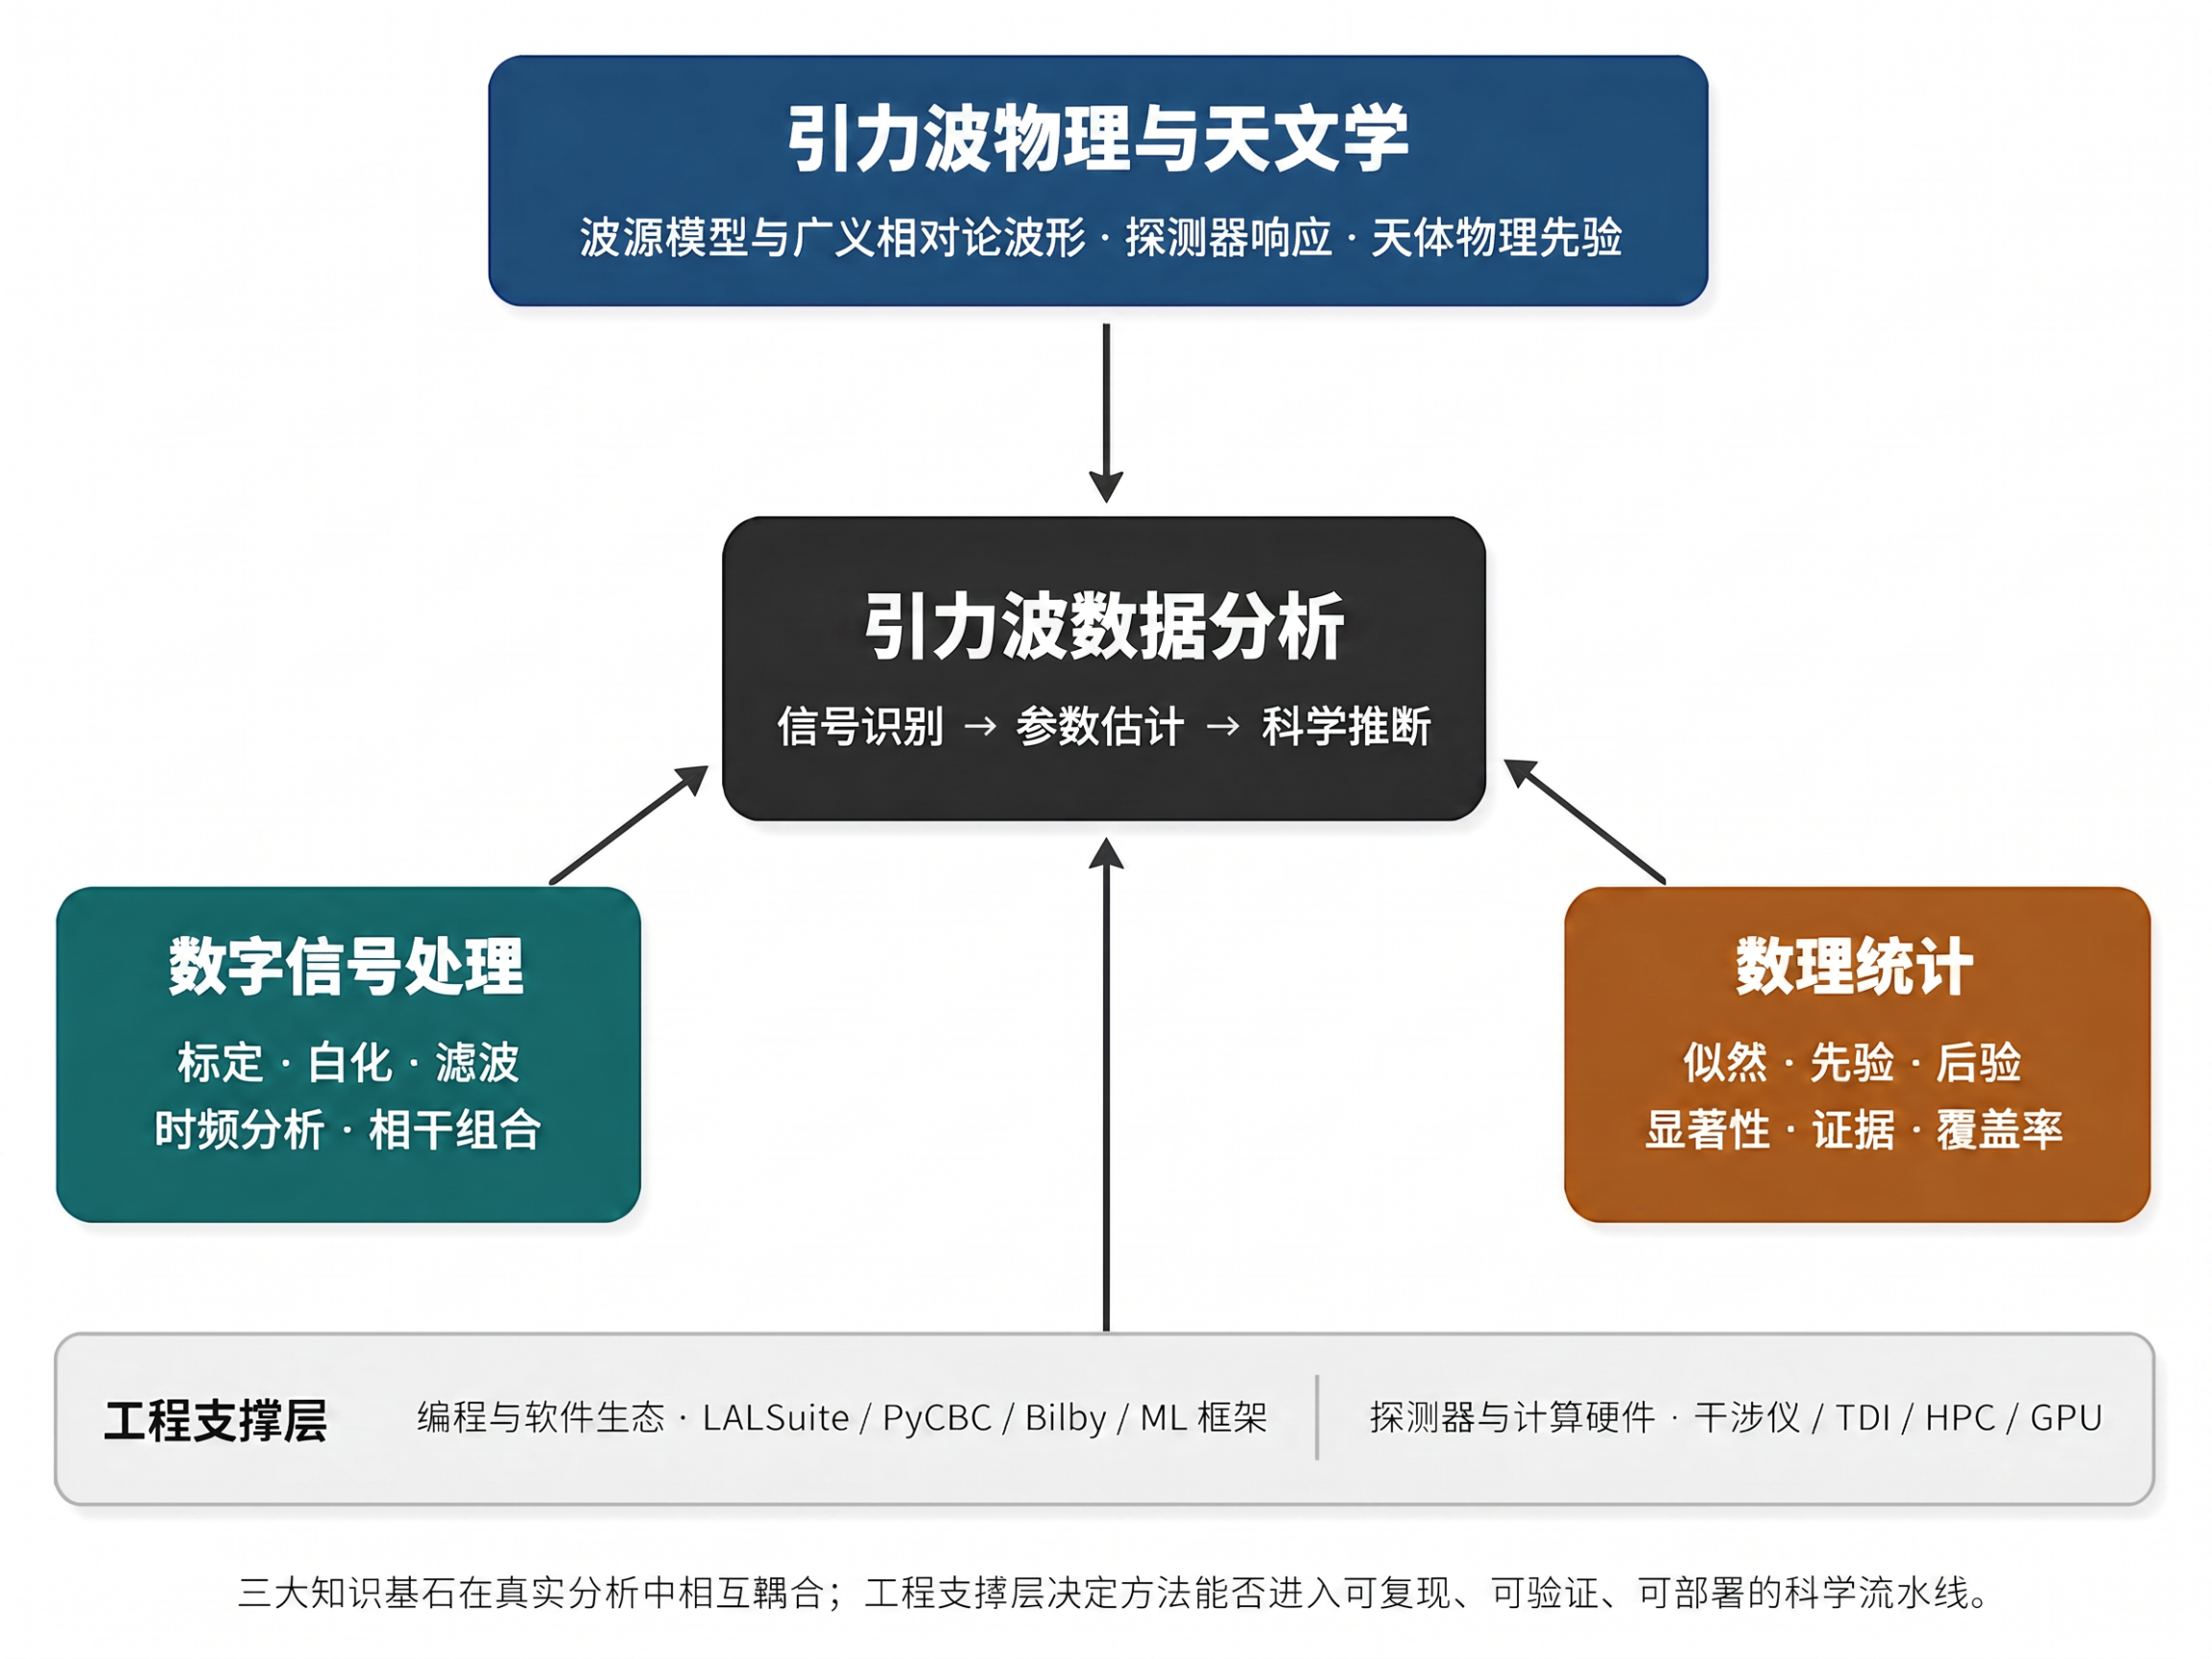
\includegraphics[width=0.92\textwidth]{figures/gw_knowledge_framework.png}
\caption{引力波数据分析的知识框架及其工程支撑。引力波物理与天文学、数字信号处理和数理统计构成三大知识基石，编程与软件生态、探测器与计算硬件构成工程支撑层；真实分析任务在三者交界处完成信号识别、参数估计和科学推断。}
\label{fig:gw_knowledge_framework}
\end{figure}

\textbf{核心创新点}包括以下五个方面：

其一，\textbf{物理驱动的网络设计}：感知层 CNN 将匹配滤波的物理先验以归纳偏置的形式嵌入网络结构（第5章），先验知识采样策略将物理先验转化为训练数据分布设计（第6章），两者共同构成“物理-数据融合”的早期实践。这一创新的核心洞察在于：引力波信号的物理特征（啁啾频率演化、特征时频轨迹、极化模式）可以通过网络结构设计而非仅靠数据学习来编码，从而在有限训练样本下实现更好的泛化性能，并赋予网络决策过程以物理可解释性。具体而言，MF-CNN 的感知层卷积核被初始化为匹配滤波模板的形状，使网络在训练初期就具备了物理意义明确的特征提取能力，而非从随机初始化出发盲目学习。

其二，\textbf{空间引力波参数估计的系统性突破}：归一化流和连续归一化流方法在太极任务的大质量双黑洞和极端质量比旋入参数估计中，实现比传统 MCMC 方法快几个数量级的推断速度（第6章），其中 EMRI 17 维参数空间的机器学习参数估计探索具有里程碑意义。传统的 MCMC 方法（如 Nested Sampling）对单个 EMRI 事件的参数估计需要大量波形计算，每次高保真波形计算可能耗时较长，总计算时间可达月级。归一化流方法通过一次性训练，将后验分布的采样时间压缩至秒级乃至更短时间尺度。这一加速不仅使低延迟参数估计成为可能，更为空间引力波全局拟合中的迭代优化提供了可行的计算基础。

其三，\textbf{Transformer 架构的引力波去噪}：WaveFormer 将自注意力机制引入引力波信号去噪，克服 CNN 的长程依赖局限（第7章）；针对空间探测器非稳态噪声的鲁棒去噪方法，为真实探测管道的构建提供了方法论基础。引力波信号的旋进阶段持续时间可达数分钟至数小时（对于低质量系统），信号的早期部分（低频、低振幅）与晚期部分（高频、高振幅）之间存在强烈的长程相关性——早期的频率演化速率决定了晚期的并合时刻，这种全局相关性是 CNN 等局部感受野方法难以有效捕捉的。Transformer 的自注意力机制天然适合处理这种长程依赖，WaveFormer 的实验结果表明，在相同参数量下，Transformer 架构的去噪性能显著优于 CNN，尤其在低信噪比条件下优势更为明显。

其四，\textbf{LLM 驱动的可解释算法自动发现}：Evo-MCTS 框架将大语言模型、蒙特卡洛树搜索与进化计算三者有机整合，在 MLGWSC-1 基准上超越强挑战赛基线 20.2\%，同时保持算法的物理可解释性（第8章）。这是 LLM 驱动的自动算法发现在引力波检测任务中的系统性实践。传统的神经架构搜索（NAS）和超参数优化方法通常将算法视为黑箱，优化目标是性能指标，而不关心算法的物理意义。Evo-MCTS 的创新在于：利用 LLM 的代码生成能力在算法空间中进行有意义的探索（而非随机变异），利用蒙特卡洛树搜索在算法演化树中进行有效的规划，利用进化计算维持算法多样性并避免局部最优。最终发现的算法不仅性能优越，而且其每一步操作都有明确的物理解释，可以被领域专家理解和验证。

其五，\textbf{方法论的跨领域普适性}：SBI 方法从引力波参数估计迁移到 21cm 森林宇宙学观测（第11章），beyond-GR 信号探测展示了 AI 作为理论无关探测器的潜力（第11章），共同指向 AI 方法在天文学中的更广泛应用前景。21cm 森林是高红移宇宙中性氢对背景射电源的吸收特征，其功率谱携带了宇宙再电离历史和暗物质性质的信息，但正向模拟极为耗时，传统的 MCMC 参数估计面临与引力波 EMRI 类似的计算瓶颈。将 SBI 方法迁移到这一领域，不仅解决了具体的计算问题，更验证了 SBI 作为通用推断框架的跨领域适用性，为 AI 方法在更广泛的天文学问题中的应用提供了方法论范本。

本书的组织结构遵循“问题驱动、方法递进、应用验证”的逻辑：第一、二部分建立理论基础和传统方法的参照系，第三、四部分系统介绍 AI 新方法及其与物理的融合，第五部分面向未来空间任务和发展趋势。每章均以具体的科学问题为起点，以定量的实验结果为支撑，以与全书论点的关联为收尾，形成完整的逻辑闭环。

表~\ref{tab:original_contributions}列出了与本书主题密切相关、作者参与完成的代表性研究工作。这些研究均依托具体合作团队开展，其中既包括作者主导或共同主导的工作，也包括作者作为合作者参与推进的重要成果；表中所称“贡献”指相关论文或项目对本书方法论主线的贡献，而非表示所有工作均为作者单独完成。

\begin{table}[htbp]
\centering
\caption{作者参与和合作完成的重要研究工作汇总}
\label{tab:original_contributions}
\small
\begin{tabular}{lllc}
\hline
\textbf{研究工作} & \textbf{核心贡献} & \textbf{对应章节} & \textbf{参考文献} \\
\hline
MF-CNN & 物理先验嵌入CNN，较早在真实LIGO-Virgo数据中系统应用 & 第5章 & \cite{wang2020deeplearning} \\
先验知识采样 & 物理先验引导的归一化流训练策略 & 第6章 & \cite{wang2022normflow} \\
太极归一化流 & 太极MBHB参数估计，处理时变响应函数 & 第6章 & \cite{du2024normflow} \\
CNF-MBHB & 流匹配CNF用于太极MBHB参数估计 & 第6章 & \cite{liang2024cnfmbhb} \\
CNF-EMRI & ML方法用于EMRI 17维参数估计探索 & 第6章 & \cite{liang2024cnfemri} \\
CVAE混合推断 & CVAE+贝叶斯精确协同，压缩至14\%时间 & 第6章 & \cite{sun2025cvae} \\
SBI综述 & SBI方法在引力波数据分析中的系统综述 & 第6章 & \cite{liang2026sbireview} \\
WaveFormer & Transformer架构引力波去噪 & 第7章 & \cite{wang2024waveformer} \\
长时序列去噪 & 30天旋近信号去噪与并合时刻预测 & 第7章 & \cite{xu2024denoising} \\
鲁棒去噪 & 非稳态噪声鲁棒深度学习去噪 & 第7章 & \cite{xu2024nonstationarty} \\
Evo-MCTS & LLM驱动自动算法发现，超越MLGWSC-1基线 & 第8章 & \cite{wang2025evomcts} \\
G-LNS & LLM引导大邻域搜索 & 第8章 & \cite{zhao2025glns} \\
Beyond-GR & AI作为理论无关引力波探测器 & 第11章 & \cite{wang2025beyondgr} \\
21cm SBI & SBI方法迁移至21cm森林宇宙学推断 & 第11章 & \cite{sun2025_21cm} \\
太极挑战综述 & 太极数据分析挑战与AI方法综述 & 第10章 & \cite{wang2024challenges} \\
\hline
\end{tabular}
\par\vspace{2mm}
\parbox{0.96\textwidth}{\zihao{-5}\textbf{说明：}本表仅用于说明这些合作研究与本书各章论述之间的对应关系。表中工作包含多位合作者和合作团队的共同贡献，具体作者排序、贡献分工和资助背景以相应论文原文为准。}
\end{table}

\section{本书章节安排}

本书共分五个部分、十二章，各章内容安排如下。

\textbf{第一部：理论基础与背景（第1--2章）}

第1章（绪论）系统梳理引力波天文学的历史脉络与探测现状，介绍地面和空间引力波探测器的技术特点与科学目标，分析数据分析面临的三层挑战（信号识别、参数估计、全局拟合），并概述本书的研究主题与五项核心创新点。

第2章（引力波信号与噪声建模）建立全书的物理与数学基础，系统介绍引力波波形模型（后牛顿近似、啁啾质量、SPA频域表示）、多类型引力波源的信号特征、探测器噪声的统计性质（功率谱密度、非高斯暂态、非平稳漂移），以及数据预处理的标准流程。

\textbf{第二部：传统方法与局限（第3--4章）}

第3章（经典的引力波数据分析方法）系统介绍匹配滤波与模板库构建、PyCBC/GstLAL 实际搜索流水线、贝叶斯推断与参数估计框架，以及蒙特卡洛采样方法的原理与实践挑战，并通过 MLGWSC-1 评测结果客观定位经典方法的性能边界。

第4章（高维参数空间与多模态挑战）从维度灾难、多源信号重叠、非平稳噪声三个维度定量分析经典方法在面向空间引力波探测器时的可扩展性瓶颈，为后续各章 AI 方法的引入提供清晰的问题动机。

\textbf{第三部：人工智能新方法（第5--7章）}

第5章（机器学习在引力波信号识别中的应用）以 MF-CNN 为核心，系统介绍卷积神经网络在引力波信号识别中的应用进展，包括感知层物理先验嵌入、集成学习、空间引力波多源统一检测、CNN 超参数调优、beyond-GR 信号探测，以及多角度可解释性分析。

第6章（生成模型与模拟推断）系统介绍模拟推断（SBI）的理论框架与主要变体（NPE/NRE/NLE），展示归一化流、连续归一化流（CNF）和混合推断策略在大质量双黑洞、极端质量比旋入参数估计中的系统应用，以及 SBI 方法向 21cm 森林宇宙学观测的跨领域迁移。

第7章（智能化信号分离与去噪）介绍 WaveFormer（Transformer 架构去噪）、长时旋近去噪与并合时刻预测、以及空间探测器非稳态噪声下的鲁棒信号提取，直接连接多信使天文学的实际预警需求。

\textbf{第四部：综合创新与融合（第8--9章）}

第8章（智能化启发式搜索与优化方法）介绍 LLM 驱动的自动算法发现方法演进（FunSearch→EoH→ReEvo→Evo-MCTS），重点展示 Evo-MCTS 在 MLGWSC-1 基准上超越强基线 20.2\% 的系统性验证，以及领域知识集成与可解释算法路径的关键作用。

第9章（物理驱动与数据驱动的融合方法）从互补缺陷分析出发，系统梳理物理先验嵌入、混合推断（精确协同）、可解释性验证三条融合路径，提出“精确协同”而非“近似替代”的方法论范式。

\textbf{第五部：前沿挑战与展望（第10--12章）}

第10章（未来空间引力波探测任务的数据挑战）以太极任务为主线，系统分析全局拟合的终极挑战、AI 方法在各类源分析中的分层角色、非稳态噪声的系统性处理，以及高保真仿真与真实探测管道的构建要素。

第11章（智能化引力波天文学的发展趋势）从四个维度展望 AI 在科学研究中角色的转变：LLM 驱动的自动算法发现、SBI 方法的跨领域迁移、AI 作为理论无关探测器，以及持续智能监测与人机协作的未来形态。

第12章（结语）以三条方法论主线（黑箱→可解释、近似替代→精确协同、单一方法→自动发现）总结全书贡献，并指出空间引力波全局拟合可行化、SBI 精度保证框架、AI 驱动科学发现泛化边界三个核心开放问题。

引力波天文学的独特地位在于，它是少数几个同时满足“物理理论极为精确”（广义相对论提供精确波形预言）和“信号检测极为困难”（应变灵敏度约$10^{-23}$）的科学领域，这一组合使它成为检验数据分析方法论的理想试验场：任何声称“有效”的方法都必须在极端噪声条件下通过严格的统计检验；任何声称“物理一致”的AI方法都可以通过对比理论预言来客观验证。这种近乎苛刻的科学标准，是引力波数据分析方法论研究的独特价值——在这里产生的方法论创新，往往具有超越引力波领域本身的普适性，因为它们是在最严格的科学标准下锻造出来的。

本书各章的内容组织遵循“从已知到未知、从经典到前沿、从单一到融合”的认知递进逻辑。第一部建立物理基础（读者需要的物理背景），第二部分析经典方法的能力与局限（为什么需要AI方法），第三部系统介绍AI新方法（怎么用AI方法），第四部展示融合与创新（怎么做到更好），第五部展望未来（下一步往哪里走）。这一逻辑链条不是线性阅读的约束，而是理解全书方法论体系的骨架。读者可以根据自己的知识背景选择合适的入口，但理解每章内容与整体框架的关联，是获得本书最大价值的关键。

\textbf{本书在线开源版本}已公开发布，欢迎在线阅读与交流：
\begin{center}
\url{https://iphysresearch.github.io/gwai-monograph/}
\end{center}
在线版与本书同步，支持全文检索和章节导航，并开放读者评论与勘误提交。

\section{本章小结}

本章从引力波天文学的历史脉络出发，系统梳理了从爱因斯坦1916年的理论预言到2015年 GW150914 首次直接探测的百年历程。Hulse-Taylor 脉冲双星 PSR B1913+16 的发现与轨道周期衰减的精密测量，提供了引力波存在的第一个间接证据，其与广义相对论预言的符合精度优于0.3\%，坚定了物理学界直接探测引力波的信心。LIGO 从1984年的构想到2002年初代运行、再到2015年 Advanced LIGO 的历史性突破，是科学史上长期愿景与技术攻关的典范。GW150914 的每一个观测细节——35至150 Hz 的啁啾频率演化、$10^{-21}$ 的峰值应变、7毫秒的两台探测器时延、5.1$\sigma$ 的统计显著性——都承载着深刻的物理意义，标志着引力波天文学新时代的开启。O1--O3 已公开近百个引力波候选事件，O4 进一步扩展样本规模；从 GW170817 的多信使天文学到 GW190521 的中间质量黑洞候选体，引力波天文学正在从“单次发现”迈向“海量统计”的大数据时代。

在探测器技术方面，Advanced LIGO 的臂腔（精细度约450，臂腔功率约750 kW）、信号循环腔、四级悬挂隔振系统和量子压缩光技术代表了当代精密测量的最高水平。下一代地面探测器（ET 的10公里三角形地下构型、CE 的40公里L型构型）将把灵敏度再提升一个量级，实现宇宙学距离上的引力波天文学。空间探测器（LISA、太极、天琴）将把探测窗口延伸至毫赫兹频段，探测超大质量黑洞并合、EMRI 和银河系双白矮星，三个任务的联合观测将大幅提升天空定位精度和参数估计精度。

在数据分析挑战方面，信号搜索面临极弱应变信号（典型量级 $\sim10^{-23}$）、非高斯 glitch（每小时数个至数十个）、非平稳噪声和高维参数空间（BBH 约15维，EMRI 约17维）的四重挑战；参数估计的科学价值体现在质量分布约束黑洞形成机制、自旋测量区分起源、距离测量给出哈勃常数等多个维度；空间引力波全局拟合的有效参数维度可达 $10^5$ 至 $10^7$ 量级，直接 MCMC 方法难以满足任务时效要求，是 AI 方法具有重要价值的根本动机。

本书的五项核心创新——MF-CNN 物理先验嵌入、SBI 参数估计加速、WaveFormer 智能去噪、Evo-MCTS 自动算法发现、物理-数据精确协同——均在这一问题框架下提出，构成了全书的方法论主线。理解这一框架，是把握后续各章具体方法动机的前提。

引力波天文学发展到今天，已经成为一门高度交叉的学科，其数据分析方法论的演进涉及广义相对论与天体物理学（物理建模）、统计学与贝叶斯推断（方法论基础）、信号处理与滤波（数据预处理）、机器学习与人工智能（方法革新）、以及高性能计算与软件工程（基础设施）。本书定位于方法论层面的系统梳理，不要求读者在所有五个方向都有深厚背景，但希望通过清晰的问题陈述和方法动机说明，帮助不同背景的读者在自己最熟悉的维度上理解本书的方法论贡献。对物理学家而言，重点是理解为何特定的物理先验对AI方法有决定性价值；对数学/统计学家而言，重点是理解引力波推断问题的特殊结构如何催生了SBI等新的推断范式；对计算机科学家而言，重点是理解科学约束如何重新定义了算法设计的目标和评估标准；对工程师而言，重点是理解从研究原型到生产系统的关键工程挑战。正是这种多维度的交叉融合，使引力波数据分析方法论成为科学AI方法论发展的最佳“试验场”之一。

\chapter{引力波信号与噪声建模}

引力波数据分析的所有方法——无论是传统的匹配滤波、贝叶斯推断，还是本书后续各章介绍的深度学习、模拟推断——都建立在对信号和噪声的数学描述之上。理解这些描述的物理基础，是理解后续方法选择的前提。本章系统介绍引力波信号的波形模型、源类型的多模态特征、探测器噪声的统计性质，以及数据预处理的标准流程。

\section{引力波的基本理论与波形模型}

在线性化广义相对论的弱场慢速近似下，引力波表现为时空度规的横波扰动~\cite{Einstein1916GW}。在横-无迹（TT）规范中，度规扰动为
\begin{equation}
  \mathrm{d}s^2 = -c^2\mathrm{d}t^2 + (\delta_{ij} + h_{ij}^{\mathrm{TT}})\,\mathrm{d}x^i\,\mathrm{d}x^j,
\end{equation}
其中 $h_{ij}^{\mathrm{TT}}$ 为引力波应变张量，其两个独立分量（$+$ 极化和 $\times$ 极化）描述了时空在垂直于传播方向平面内的伸缩和剪切。

\subsection{线性化广义相对论与引力波方程}

引力波的理论基础来自爱因斯坦广义相对论的线性化近似。爱因斯坦场方程的完整形式为
\begin{equation}
  G_{\mu\nu} = \frac{8\pi G}{c^4} T_{\mu\nu},
\end{equation}
其中 $G_{\mu\nu}$ 为爱因斯坦张量，$T_{\mu\nu}$ 为能量-动量张量。在弱场近似下，将时空度规写为闵可夫斯基度规加上小扰动：$g_{\mu\nu} = \eta_{\mu\nu} + h_{\mu\nu}$，其中 $|h_{\mu\nu}| \ll 1$。将此代入爱因斯坦方程并保留 $h_{\mu\nu}$ 的一阶项，得到线性化的场方程。

为简化方程，引入迹反转度规扰动 $\bar{h}_{\mu\nu} = h_{\mu\nu} - \frac{1}{2}\eta_{\mu\nu}h$（其中 $h = \eta^{\mu\nu}h_{\mu\nu}$ 为迹），并选取洛伦兹规范（Lorenz gauge）$\partial^\mu \bar{h}_{\mu\nu} = 0$，线性化场方程化为简洁的波动方程：
\begin{equation}
  \Box \bar{h}_{\mu\nu} = -\frac{16\pi G}{c^4} T_{\mu\nu},
\end{equation}
其中 $\Box = -\partial_t^2/c^2 + \nabla^2$ 为达朗贝尔算符。在真空中（$T_{\mu\nu} = 0$），此方程化为标准的波动方程 $\Box \bar{h}_{\mu\nu} = 0$，其解为以光速传播的横波——引力波。

在横-无迹（TT）规范中，通过进一步的规范选择，可以将引力波的独立自由度减少到最少。TT 规范要求 $h_{0\mu}^{TT} = 0$（时间分量为零）、$\partial^j h_{ij}^{TT} = 0$（横向条件）、$h_{ii}^{TT} = 0$（无迹条件）。在这一规范下，对于沿 $z$ 轴传播的引力波，度规扰动只有两个独立分量：
\begin{equation}
  h_{ij}^{TT} = \begin{pmatrix} h_+ & h_\times & 0 \\ h_\times & -h_+ & 0 \\ 0 & 0 & 0 \end{pmatrix} \cos(\omega t - kz),
\end{equation}
其中 $h_+$ 和 $h_\times$ 分别为两种极化模式的振幅。$h_+$ 极化描述沿 $x$-$y$ 轴方向的时空拉伸-压缩：当 $h_+ > 0$ 时，$x$ 方向拉伸、$y$ 方向压缩；当 $h_+ < 0$ 时反之。$h_\times$ 极化描述沿 $45°$ 方向的时空剪切。一个环形排列的自由质点在 $h_+$ 极化的引力波通过时，会交替地变形为沿 $x$ 方向拉长的椭圆和沿 $y$ 方向拉长的椭圆，形成特征性的“呼吸”运动。

\subsection{四极辐射公式与轨道衰减}

引力波的辐射功率由质量四极矩张量的时间导数决定。对于缓慢运动（$v \ll c$）的引力波源，辐射功率由四极公式给出：
\begin{equation}
  P = \frac{G}{5c^5} \left\langle \dddot{Q}_{ij} \dddot{Q}^{ij} \right\rangle,
\end{equation}
其中 $Q_{ij} = \int \rho(x_i x_j - \frac{1}{3}\delta_{ij}r^2)\,d^3x$ 为质量四极矩张量的无迹部分，上方三点表示对时间的三阶导数，尖括号表示对轨道周期的时间平均。这一公式揭示了引力波辐射的基本物理：只有质量分布的四极矩随时间变化才能辐射引力波，球对称或轴对称的运动（如球对称坍缩、均匀自转）不产生引力波辐射。

对于圆轨道双星系统，质量分别为 $m_1$ 和 $m_2$，轨道半径为 $r$，四极辐射功率为：
\begin{equation}
  P = \frac{32G^4}{5c^5} \frac{m_1^2 m_2^2 (m_1 + m_2)}{r^5}.
\end{equation}
这一功率来自轨道动能和引力势能的损失，导致轨道半径随时间减小（轨道衰减）。轨道衰减的速率为：
\begin{equation}
  \dot{r} = -\frac{64G^3}{5c^5} \frac{m_1 m_2 (m_1 + m_2)}{r^3},
\end{equation}
从初始轨道半径 $r_0$ 到并合（$r \to 0$）的时间尺度为 $\tau \propto r_0^4$。对于 Hulse-Taylor 脉冲双星 PSR B1913+16，轨道周期约7.75小时，轨道偏心率约0.617，理论预言的轨道周期衰减速率约为每年76微秒，与观测值的符合精度优于0.3\%，是引力波存在的最精确间接证据。

\subsection{后牛顿展开与引力波相位}

在旋进阶段，引力波波形的精确计算依赖后牛顿（post-Newtonian，PN）展开，即以 $v/c$（轨道速度与光速之比）为小参数的系统展开~\cite{Blanchet2014PN}。后牛顿展开的精度通常以 PN 阶数表示：$n$PN 阶对应 $(v/c)^{2n}$ 量级的修正。目前引力波数据分析中使用的波形模型通常精确到 3.5PN 阶（即 $(v/c)^7$ 量级），包含了质量比、对称质量比、自旋-轨道耦合、自旋-自旋耦合等多种修正项。

引力波相位的后牛顿展开在频域中具有特别简洁的形式。在驻相近似（SPA）下，频域波形的相位为：
\begin{equation}
  \Psi(f) = 2\pi f t_c - \phi_c - \frac{\pi}{4} + \frac{3}{128}(\pi \mathcal{M} f)^{-5/3} \sum_{k=0}^{7} \psi_k \left(\pi M f\right)^{k/3},
\end{equation}
其中 $t_c$ 为并合时刻，$\phi_c$ 为并合相位，$\mathcal{M}$ 为啁啾质量，$M = m_1 + m_2$ 为总质量，$\psi_k$ 为各阶后牛顿系数（依赖于质量比和自旋参数）。每个 $\psi_k$ 系数的精确值与引力理论相关，是检验广义相对论的探针：如果广义相对论在强场条件下存在偏差，这些系数将偏离广义相对论的预言值，从而在引力波相位中留下可测量的印记。

后牛顿展开的一个重要结论是啁啾质量 $\mathcal{M}$ 的主导地位：在最低阶（0PN）近似下，引力波频率演化完全由 $\mathcal{M}$ 决定，而与质量比无关。这意味着 $\mathcal{M}$ 是引力波信号中测量最精确的参数，其测量精度通常比单个天体质量高一到两个量级。对于 GW150914，$\mathcal{M} \approx 28.3\,M_\odot$ 的测量精度约为 $\pm 1.5\,M_\odot$（约5\%），而单个黑洞质量的测量精度约为 $\pm 4\,M_\odot$（约12\%）。

探测器测量的应变为
\begin{equation}
  h(t) = F_+(\alpha, \delta, \psi)\,h_+(t) + F_\times(\alpha, \delta, \psi)\,h_\times(t),
\end{equation}
其中 $F_+$、$F_\times$ 为天线响应函数，取决于源的天空位置 $(\alpha, \delta)$ 和极化角 $\psi$。

对于致密双星系统（双黑洞、双中子星），引力波波形由三个阶段组成：\textbf{旋近阶段}（inspiral）——两个天体在引力波辐射能量损失的驱动下螺旋靠近，频率单调增加，形成特征性的“啁啾”信号；\textbf{并合阶段}（merger）——两体系统的非线性动力学，需要数值相对论计算；\textbf{衰荡阶段}（ringdown）——并合后残余黑洞通过准简正模振荡辐射剩余能量，最终趋于稳态。

\begin{figure}[htbp]
\centering
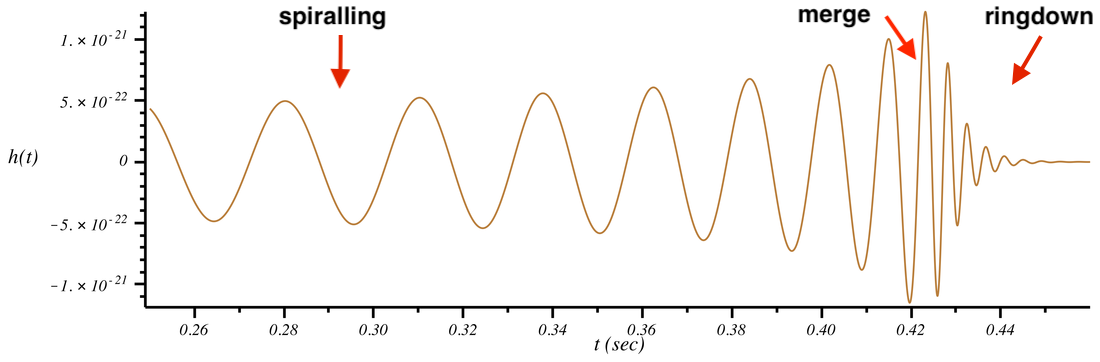
\includegraphics[width=0.96\textwidth]{figures/C2_gw_wf.png}
\caption{数值相对论波形模板在 Hanford（H1）观测站响应中的示意，对应 GW150914 型双黑洞并合事件。图中可见旋近（spiralling）、并合（merge）和衰荡（ringdown）三个阶段：频率与振幅在并合前快速增加，并合后残余黑洞以准简正模形式迅速衰减。该图引自文献资料中的 GW150914 波形模板示例~\cite{Abbott2016GW150914}。}
\label{fig:gw_waveform}
\end{figure}

实际应用中广泛使用的是现象学波形模型（IMRPhenomX 系列）和有效单体波形模型（EOBNR 系列），它们通过将后牛顿解析计算与数值相对论校准相结合，高效覆盖参数空间，构成匹配滤波模板库和贝叶斯参数估计的核心工具~\cite{Babak2017MCMC}。


\section{引力波源类型与多模态信号特征}

不同类型的引力波源在频率、持续时间、信号形态上存在显著差异，构成了信号空间的多模态结构。

\textbf{地面探测器频段（约 10 Hz--数千 Hz）}主要源类型包括：
\begin{itemize}
  \item \textit{双黑洞并合}（BBH）：最常见的观测事件类型，持续时间从数秒（高质量系统）到数分钟（低质量系统），信噪比通常较高。
  \item \textit{双中子星并合}（BNS）：持续时间更长（数分钟至数十分钟），并合后可能产生超新星和短伽马射线暴，是多信使天文学的核心目标。
  \item \textit{黑洞-中子星并合}（NSBH）：介于两者之间，若中子星被撕碎可能产生明显的电磁对应体。
\end{itemize}

\textbf{空间探测器覆盖的毫赫兹频段}的信号种类更为丰富：大质量双黑洞（$10^5$--$10^8\,M_\odot$）、极端质量比旋入（EMRI）、银河系双白矮星（数百万个同时叠加）、以及随机引力波背景。这种多源叠加的复杂性是空间引力波数据分析的核心挑战之一。

\subsection{双黑洞并合系统}

双黑洞并合（BBH）是迄今为止引力波探测中最常见的事件类型，GWTC-3 目录~\cite{Abbott2021GWTC3}中约90\%的事件为 BBH。BBH 的质量范围跨越多个量级：恒星级 BBH 的单个黑洞质量通常在 $5\,M_\odot$ 至 $100\,M_\odot$ 之间，总质量在 $10\,M_\odot$ 至 $200\,M_\odot$ 之间；中间质量 BBH（IMBHB）的质量在 $100\,M_\odot$ 至 $10^4\,M_\odot$ 之间，目前仅有少数候选体（如 GW190521，总质量约 $150\,M_\odot$，其主要成分约 $85\,M_\odot$ 落入对不稳定质量间隙）；大质量双黑洞（MBHB）的质量在 $10^4\,M_\odot$ 至 $10^9\,M_\odot$ 之间，是空间探测器（LISA/太极）的主要目标。

BBH 的形成机制是当前天体物理学的重要研究课题，主要有两类机制：孤立双星演化（isolated binary evolution）和动力学俘获（dynamical capture）。孤立双星演化机制认为，BBH 来自大质量双星系统的演化：两颗大质量恒星经历公共包层演化（common envelope evolution），轨道收缩，最终各自坍缩为黑洞，形成紧密的 BBH 系统。这一机制预言 BBH 的自旋通常与轨道角动量对齐（有效自旋参数 $\chi_\text{eff} > 0$），且质量比接近1（两个黑洞质量相近）。动力学俘获机制认为，BBH 在致密星团（球状星团、核星团）中通过引力散射形成：两个孤立黑洞在多体相互作用中被俘获为束缚系统。这一机制预言 BBH 的自旋方向随机（$\chi_\text{eff}$ 分布对称于零），且质量比分布更宽。

GWTC-3 的统计分析表明，观测到的 BBH 质量分布具有复杂结构，无法用单一的幂律分布描述：在约 $10\,M_\odot$ 处存在一个质量峰，在约 $35\,M_\odot$ 处存在另一个峰，在约 $3\,M_\odot$ 至 $5\,M_\odot$ 的“质量间隙”中存在若干候选体，在约 $50\,M_\odot$ 至 $130\,M_\odot$ 的“对不稳定质量间隙”中也有候选体（如 GW190521 的主要成分约 $85\,M_\odot$）。这些特征对黑洞形成机制提出了重要约束，也是引力波天文学与恒星演化理论交叉研究的核心问题。

\subsection{双中子星并合与多信使天文学}

双中子星并合（BNS）是引力波天文学中科学价值最丰富的事件类型之一。中子星的质量范围约为 $1.1\,M_\odot$ 至 $2.3\,M_\odot$，由核物质状态方程决定的最大质量约为 $2\,M_\odot$ 至 $3\,M_\odot$（具体值取决于状态方程）。BNS 的引力波信号持续时间远长于 BBH：对于典型的 $1.4+1.4\,M_\odot$ 系统，从进入 LIGO 灵敏频段（约10 Hz）到并合约需数分钟，在 Advanced LIGO 的灵敏频段内积累约 $10^4$ 个轨道周期，信号的相位演化携带了极为丰富的物理信息。

GW170817 是迄今唯一具有明确电磁对应体的引力波事件~\cite{Abbott2017GW170817}，其科学价值难以估量。该事件的引力波信号于2017年8月17日被 LIGO-Virgo 网络探测到，啁啾质量约为 $1.188\,M_\odot$，对应两颗中子星的质量约为 $1.17\,M_\odot$ 和 $1.60\,M_\odot$（在低自旋先验下），光度距离约为 $40^{+8}_{-14}$ Mpc，宿主星系为 NGC 4993。引力波信号结束约1.7秒后，Fermi 和 INTEGRAL 卫星探测到短伽马射线暴 GRB 170817A，强有力地支持了双中子星并合与一类短伽马射线暴之间的物理联系。此后数天至数周内，数十台光学、近红外、X射线、射电望远镜对 NGC 4993 进行了密集观测，发现了千新星（kilonova）AT2017gfo——这是重元素（如金、铂、铀）通过 r 过程核合成的重要观测证据，极大推进了宇宙重元素起源问题的研究。

BNS 并合后的产物是另一个重要的科学问题。根据并合前两颗中子星的总质量与最大中子星质量的关系，并合后可能形成：超大质量中子星（hypermassive neutron star，HMNS，寿命约数毫秒，最终坍缩为黑洞）、超稳定中子星（supramassive neutron star，寿命约数秒至数分钟或更长）、或直接坍缩为黑洞。GW170817 的后续电磁观测普遍支持其残余体在较短时间内坍缩为黑洞，但具体坍缩时刻和机制仍存在模型依赖与争议。未来的高频引力波探测（$\gtrsim 1$ kHz）将有望直接探测并合后残余体的振荡，为中子星状态方程提供更直接的约束。

\subsection{极端质量比旋入系统}

极端质量比旋入（EMRI）是空间引力波探测器最重要的科学目标之一，也是引力波数据分析中最具挑战性的问题。EMRI 系统由一个超大质量黑洞（质量 $M \sim 10^4$--$10^7\,M_\odot$）和一个轨道星体（质量 $\mu \sim 1$--$100\,M_\odot$，通常为中子星、白矮星或恒星级黑洞）组成，质量比 $q = \mu/M \sim 10^{-4}$--$10^{-7}$。

EMRI 的引力波信号具有极为丰富的物理内容。由于质量比极小，轨道星体对中心黑洞的反作用可以忽略，其轨道运动精确地追踪 Kerr 时空的测地线。在 LISA/太极的灵敏频段内，一个典型的 EMRI 事件在并合前约一年内会经历约 $10^5$ 个轨道周期，每次绕转产生的引力波相位变化与 Kerr 时空的几何精密相关。这意味着 EMRI 信号是对中心黑洞时空几何的极精密测绘：通过精确测量 EMRI 的引力波相位演化，可以以前所未有的精度测量中心黑洞的质量和自旋，检验“黑洞无毛定理”（即 Kerr 度规完全由质量和自旋描述），以及探测中心黑洞周围可能存在的暗物质晕或其他物质分布。

EMRI 信号的数据分析极为困难。首先，信号持续时间长（约一年），在频域中形成极为密集的谱线结构，与其他信号高度重叠。其次，EMRI 的参数空间约17维（中心黑洞质量和自旋、轨道星体质量、轨道偏心率、轨道倾角、初始相位等），且参数之间存在强简并。第三，高保真 EMRI 波形需要描述 Kerr 时空中的相对论轨道演化、引力辐射反作用和多谐波结构，计算代价远高于常规双黑洞波形。这些困难使得直接模板库搜索和常规逐点采样在 EMRI 问题中面临严峻压力，也使机器学习方法（特别是模拟推断）成为空间引力波数据分析中的重要候选路线。

\subsection{随机引力波背景}

随机引力波背景（SGWB）是由大量不可分辨的引力波源叠加形成的弥漫性背景辐射，类似于宇宙微波背景辐射（CMB）在引力波领域的对应物。SGWB 的来源可分为天体物理起源和宇宙学起源两大类。

天体物理起源的 SGWB 主要来自宇宙历史上所有双致密星并合事件的叠加。在地面探测器（LIGO/Virgo/KAGRA）频段，BBH 并合产生的背景能量密度约为 $\Omega_{GW} \sim 10^{-9}$（以临界密度为单位），目前尚未被探测到，但在 O4/O5 期间有望达到探测阈值。在 LISA 频段，银河系内不可分辨的双白矮星形成的混叠背景（confusion noise）是数据分析的主要挑战之一，其能量密度约为 $\Omega_{GW} \sim 10^{-11}$--$10^{-10}$，在 $1$--$10$ mHz 频段显著高于仪器噪声。

宇宙学起源的 SGWB 携带了宇宙早期历史的信息，是引力波宇宙学的核心目标。一阶宇宙相变（如电弱相变或 QCD 相变）产生的 SGWB 来自相变泡泡的碰撞和磁流体动力学湍流，其特征频率和能量密度取决于相变温度和强度，在 LISA 频段可能产生可探测的信号。宇宙弦（cosmic strings）产生的 SGWB 来自宇宙弦环的振荡和湮灭，其功率谱具有特征性的平坦形状，在宽频段内均有贡献。原初引力波（primordial gravitational waves）是宇宙暴胀期间产生的张量扰动，其功率谱由张量-标量比 $r$ 描述，目前的 CMB 观测给出 $r < 0.06$，对应的 SGWB 能量密度约为 $\Omega_{GW} \sim 10^{-16}$，远低于当前和近期探测器的灵敏度，但未来的空间探测器（如 BBO 或 DECIGO）有望探测到。

\textbf{SGWB 的探测方法}。SGWB 的探测面临独特的方法论挑战：背景信号本身是随机的，无法通过单次观测确认，必须通过统计方法从噪声中提取。标准方法是跨探测器互相关（cross-correlation）：对于两台探测器 $i$ 和 $j$，互相关统计量为
\begin{equation}
  \hat{C}_{ij}(f) = \frac{2}{T} \tilde{d}_i^*(f) \tilde{d}_j(f),
\end{equation}
其中 $T$ 为观测时间，$\tilde{d}$ 为频域数据。在高斯噪声假设下，$\hat{C}_{ij}$ 的期望值正比于 SGWB 的能量密度谱 $\Omega_{GW}(f)$，而噪声贡献在两台独立探测器之间不相关，因此通过长时间积分可以将信噪比提升至 $\text{SNR} \propto \sqrt{T}$。对于 LIGO 双探测器网络，探测 $\Omega_{GW} \sim 10^{-9}$ 的背景需要约一年的观测时间。

\textbf{AI 方法在 SGWB 分析中的应用}。传统互相关方法假设 SGWB 是各向同性的，但实际的天体物理背景（如 BBH 并合背景）可能具有各向异性，反映了宇宙大尺度结构的分布。深度学习方法可以通过学习背景信号的统计特征，在不假设各向同性的前提下提取 SGWB 的方向信息，这是传统方法难以实现的。此外，SBI 方法可以直接对 SGWB 的物理参数（如相变温度、宇宙弦张力）进行贝叶斯推断，绕过传统方法中对似然函数解析形式的依赖，为宇宙学参数约束提供更灵活的推断框架。

\textbf{脉冲星计时阵列（PTA）的纳赫兹背景}。2023年，多个脉冲星计时阵列（PTA）合作组——包括北美纳赫兹引力波天文台（NANOGrav）、欧洲脉冲星计时阵列（EPTA）、印度脉冲星计时阵列（InPTA）和帕克斯脉冲星计时阵列（PPTA）——相继报告了纳赫兹频段随机引力波背景的候选信号，其能量密度约为 $\Omega_{GW} \sim 10^{-9}$，频率约为 $10^{-9}$--$10^{-7}$ Hz。这一信号的物理起源尚不确定，候选解释包括超大质量双黑洞并合背景、宇宙弦网络、以及早期宇宙相变。PTA 的发现与 LISA/太极的毫赫兹频段观测形成互补，共同构成了多频段引力波宇宙学的观测基础。AI 方法在 PTA 数据分析中同样发挥着重要作用：机器学习方法被用于脉冲星计时残差的噪声建模、信号与噪声的分离，以及宇宙学参数的贝叶斯推断。

\subsection{银河系双星与混叠噪声}

银河系内存在约 $10^7$--$10^8$ 个双白矮星系统，其中大约 $10^4$ 个在 LISA/太极的灵敏频段（$1$--$10$ mHz）内可分辨，其余形成无法单独区分的“混叠噪声”背景。这一背景在低频段（$f \lesssim 3$ mHz）的能量密度高于仪器噪声，是空间引力波探测器数据分析的主要干扰源之一。

混叠噪声的统计特性与仪器噪声不同：它具有已知的频谱形状（由银河系双星种群的统计分布决定），且在银道面方向具有各向异性。这些特性使得混叠噪声既是科学目标（通过统计分析可以约束银河系双星种群的演化历史），也是数据分析的挑战（需要与仪器噪声和其他信号源同时建模）。

全局拟合框架（第10章）的核心任务之一，就是同时估计混叠噪声的统计参数和可分辨双星的物理参数，这要求在 $10^4$ 维以上的参数空间中进行联合贝叶斯推断。AI 方法——特别是 SBI 和快速参数估计方法——是使这一任务在计算上可行的关键技术支撑。

\section{探测器噪声性质}

探测器输出 $d(t) = h(t) + n(t)$ 中，噪声 $n(t)$ 的统计性质对数据分析方法的选择有决定性影响~\cite{Christensen2022noise}。

\textbf{功率谱密度（PSD）}是描述噪声频率特性的核心量：
\begin{equation}
  \langle\tilde{n}(f)\tilde{n}^*(f')\rangle = \frac{1}{2}S_n(f)\,\delta(f - f'),
\end{equation}
其中 $S_n(f)$ 为单边功率谱密度。在高斯平稳噪声假设下，$S_n(f)$ 完全描述了噪声的统计特性，匹配滤波在此假设下达到理论最优信噪比。

然而，真实探测器噪声远比高斯平稳假设复杂：

\textbf{非高斯成分}：探测器噪声中包含大量来自环境和仪器的暂态噪声（glitch），其幅度可比背景噪声高数个量级，持续时间从毫秒到数秒不等~\cite{Nuttall2018glitch}。glitch 的形态多样（“blip”、“koi fish”、“scattered light”等），统计上不满足高斯分布，是引力波搜索中误报率的主要来源。

\textbf{非平稳性}：探测器灵敏度随时间缓慢变化（“漂移”），在特定时段也会出现突发性的灵敏度下降~\cite{Buikema2020O3noise}。这要求数据分析算法能够实时估计和追踪噪声功率谱，而非使用固定的噪声模型。

\textbf{频谱线}：地面振动、电源频率（50/60 Hz 及其谐波）、悬挂系统共振等产生的窄带频谱线，在功率谱中形成锐峰，需要专门处理~\cite{Covas2018lines}。

\begin{figure}[htbp]
\centering
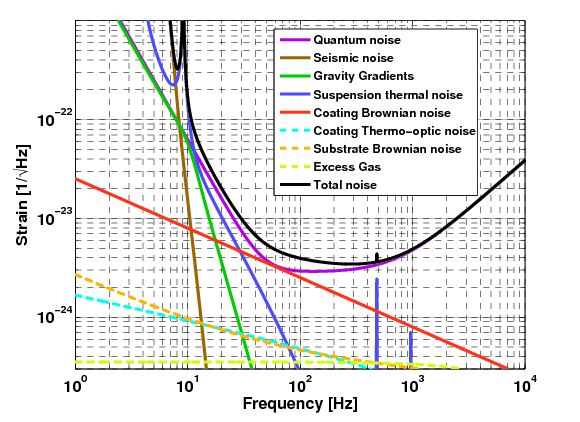
\includegraphics[width=0.82\textwidth]{figures/C2_ALIGO_broadband.png}
\caption{Advanced LIGO 中多种已知噪声来源对应的振幅谱密度。低频端主要受地震噪声、悬挂热噪声和重力梯度噪声限制，中频段由镜面与涂层热噪声等因素贡献，高频端则逐渐由量子噪声主导；黑色曲线表示各噪声项合成后的总噪声预算。图引自 Advanced LIGO 噪声预算资料，用于说明不同物理噪声源对探测器灵敏度曲线的分频段贡献~\cite{LIGOScientific2015detector}。}
\label{fig:noise_psd}
\end{figure}

量子散粒噪声（quantum shot noise）是地面引力波探测器高频灵敏度的根本限制，来源于光子计数的量子统计涨落。在相干态激光照射下，光子到达探测器的时间服从泊松分布，单位时间内的光子数涨落为 $\Delta N \sim \sqrt{N}$，对应的相位测量不确定度为 $\Delta\phi \sim 1/\sqrt{N}$。对于功率为 $P$ 的激光，单位时间内的光子数为 $N = P/(\hbar\omega)$，因此散粒噪声引起的应变噪声谱密度为：
\begin{equation}
  \sqrt{S_n^{shot}(f)} \propto \frac{1}{\sqrt{P_{circ}}} \cdot \frac{1}{L},
\end{equation}
其中 $P_{circ}$ 为臂腔内的循环光功率，$L$ 为臂长。这解释了为何 Advanced LIGO 要将臂腔功率提升至约750 kW——功率越高，散粒噪声越低。

与散粒噪声相对的是辐射压力噪声（radiation pressure noise）：高功率激光的光子动量涨落对镜面施加随机力，产生镜面位移噪声，其谱密度为：
\begin{equation}
  \sqrt{S_n^{rad}(f)} \propto \frac{\sqrt{P_{circ}}}{M f^2 L},
\end{equation}
其中 $M$ 为镜面质量。散粒噪声随功率增加而减小，辐射压力噪声随功率增加而增大，两者之积受海森堡不确定性原理约束，存在一个最优功率使总量子噪声最小——这就是标准量子极限（SQL）。在 SQL 处，散粒噪声与辐射压力噪声相等，总量子噪声为：
\begin{equation}
  \sqrt{S_n^{SQL}(f)} = \sqrt{\frac{8\hbar}{M(2\pi f)^2 L^2}}.
\end{equation}
突破 SQL 需要使用量子压缩光（squeezed light）技术：通过注入频率压缩态的真空场，可以在牺牲一个正交分量的不确定度的同时，降低另一个正交分量（相位或振幅）的不确定度，从而在特定频段将量子噪声降低至 SQL 以下。Advanced LIGO 在 O3 期间已成功实现约3 dB 的量子压缩，将高频灵敏度提升约40\%。

量子压缩光的物理机制需要更细致的说明。散粒噪声与辐射压力噪声在本质上来源于同一光场的量子涨落，两者的谱密度乘积受海森堡不确定性关系约束：$S_{shot}(f) \cdot S_{rp}(f) \geq \hbar^2/M^2L^2$，其几何均值即为标准量子极限处的总量子噪声。注入频率相关的压缩真空（frequency-dependent squeezed vacuum）可以对不同频率实现不同方向的压缩：在高频段（散粒噪声主导）压缩相位分量，在低频段（辐射压力噪声主导）压缩振幅分量。频率相关压缩需要一个滤波腔（filter cavity）来实现频率依赖的旋转角，Advanced LIGO 在 O4 运行中引入了长约300米的滤波腔，实现了频率相关压缩，在全频段量子噪声均低于 SQL。

在数据分析的视角下，量子噪声的优化与AI方法存在一个有趣的协同效应。量子压缩光降低散粒噪声的同时提升了高频灵敏度，这对高质量双黑洞并合（并合阶段频率$>100$ Hz）和双中子星合并（GW频率可达几kHz）的探测尤为重要。灵敏度提升后，在相同观测时间内可以探测到更远距离的事件，使引力波天文学的有效体积扩大，探测率相应提升。对数据分析算法而言，更高灵敏度意味着事件的平均信噪比更高，参数估计的精度更好；同时也意味着非高斯噪声（glitch）在高信噪比区域的相对贡献更大（因为真实信号变得更明显，而glitch的幅度分布不随探测器升级而改变）。这种“信号增强、glitch相对显眼”的效应，对机器学习方法的训练策略有直接影响：随着探测器升级，训练数据中的信噪比分布应相应调整，对高信噪比事件的训练权重可适当降低，同时加强对低信噪比但物理参数极端（如高质量比、高自旋）的事件的训练覆盖。这种“训练数据与探测器灵敏度协同演化”的策略，是AI方法在引力波领域持续保持高性能的关键工程实践。

从信息论角度理解量子极限：引力波探测本质上是测量两个检验质量之间的相对位移，这一测量行为不可避免地对被测系统施加反作用（辐射压力），这正是量子测量的反作用噪声。在标准量子力学框架下，任何不打破海森堡不确定性关系的测量方案都不能同时将位移分辨率和反作用力降至 SQL 以下。但通过“量子背作用规避”（quantum back-action evasion）技术——例如速度计方案（speed-meter）或变形探测器方案（variational readout）——可以在原理上规避辐射压力的反作用效应，从而使灵敏度突破 SQL。这类方案目前正在原型探测器上验证，未来的爱因斯坦望远镜（ET）和宇宙探测者（CE）计划引入这些技术，以期在全频段超越 SQL。

从实践角度，O3期间Advanced LIGO实现的约3 dB量子噪声降低，对应信噪比提升约$\sqrt{2}$倍，即灵敏度提升约40\%。这一提升意味着探测器对引力波事件的探测距离增加约26\%，对应探测体积增加约71\%（体积正比于距离的三次方）。从O2到O3期间，量子压缩的应用是引力波事件率从约10个/观测期增至约40个/观测期的重要技术因素之一，体现了量子光学技术在引力波天文学中的直接科学价值。

\subsection{热噪声与低温技术}

热噪声是地面引力波探测器中频段（约10至200 Hz）灵敏度的主要限制，来源于探测器各机械部件的热涨落。根据涨落-耗散定理，处于温度 $T$ 的机械系统的位移噪声谱密度为：
\begin{equation}
  S_x^{th}(f) = \frac{4k_B T}{\omega} \text{Im}[\chi(\omega)],
\end{equation}
其中 $\chi(\omega)$ 为系统的机械导纳（susceptibility），$\text{Im}[\chi(\omega)]$ 正比于机械损耗。这一公式揭示了降低热噪声的两条路径：降低温度 $T$，或降低机械损耗（提高机械品质因子 $Q$）。

Advanced LIGO 采用熔融石英（fused silica）纤维悬挂镜面，熔融石英在室温下的机械品质因子约为 $10^7$，是目前已知机械损耗最低的材料之一。镜面涂层（高反射率介质膜）的机械损耗是热噪声的主要来源，其品质因子约为 $10^4$，比基底低三个量级，是当前热噪声研究的核心问题。

KAGRA 采用了低温（约20 K）蓝宝石镜面，利用低温下材料机械损耗的显著降低来减小热噪声。蓝宝石在20 K 时的机械品质因子约为 $10^8$，比室温高约一个量级，理论上可将热噪声降低约3倍。低温技术的挑战在于：需要将约40公斤的镜面冷却至20 K，同时保持极低的振动水平，这需要专门设计的低温悬挂系统和辐射冷却方案。爱因斯坦望远镜（ET）计划采用约10 K 的硅镜面，将热噪声进一步降低约一个量级，使中频段灵敏度达到 $10^{-25}/\sqrt{\text{Hz}}$ 量级。

\subsection{重力梯度噪声与地下探测器}

重力梯度噪声（Newtonian noise，NN）是地面引力波探测器低频灵敏度的根本性限制，其物理机制与其他噪声源有本质区别：它不是通过机械耦合传递到检验质量，而是通过引力直接作用于检验质量，因此无法通过任何机械隔振手段消除。

重力梯度噪声的来源包括：地震波（P 波和 S 波）引起的地面密度涨落，在检验质量周围产生随时间变化的引力梯度；大气压力波（声波和重力波）引起的大气密度涨落，同样产生引力梯度；以及人类活动（车辆、机械振动）引起的局部密度涨落。在地面探测器的典型运行环境中，重力梯度噪声在约1至10 Hz 频段的贡献约为 $10^{-20}$--$10^{-19}\,\text{m}/\sqrt{\text{Hz}}$，远高于 Advanced LIGO 的设计灵敏度，是地面探测器低频截止（约10 Hz）的根本原因。

减小重力梯度噪声的主要方法有两种。第一种是在线减除（online subtraction）：在检验质量周围布置密集的地震传感器和气压传感器网络，实时测量引力梯度的涨落，然后从数据中减去其对检验质量位移的贡献。这一方法在理论上可将重力梯度噪声降低约一个量级，但实际效果受限于传感器的覆盖密度和测量精度。第二种是地下建设：将探测器建于地下数百米深处，利用岩层对地震波的天然衰减（约每100米衰减一个量级）来降低地震噪声，从而间接降低重力梯度噪声。爱因斯坦望远镜（ET）和 KAGRA 均采用了地下建设方案，ET 的设计深度约为100至200米，预计可将重力梯度噪声降低约两个量级，使低频截止降至约2至3 Hz。

\section{信号与噪声的数学建模方法}

引力波数据分析的标准内积定义为~\cite{Cutler1994PE}
\begin{equation}
  \langle a, b\rangle = 4\,\mathrm{Re}\int_0^\infty \frac{\tilde{a}(f)\tilde{b}^*(f)}{S_n(f)}\,\mathrm{d}f,
\end{equation}
这一定义使得在高斯平稳噪声下，$\langle n, n\rangle$ 服从 $\chi^2$ 分布，为统计检验提供了理论基础。

信号的最优信噪比（SNR）定义为
\begin{equation}
  \rho_\mathrm{opt} = \sqrt{\langle h, h\rangle} = \sqrt{4\int_0^\infty \frac{|\tilde{h}(f)|^2}{S_n(f)}\,\mathrm{d}f},
\end{equation}
它决定了特定信号在给定噪声背景下能够被探测到的理论极限。

在引力波参数估计中，贝叶斯似然函数的标准形式为~\cite{Veitch2015LALInference,Ashton2019Bilby}
\begin{equation}
  \ln p(d|\theta) = -\frac{1}{2}\langle d - h(\theta), d - h(\theta)\rangle + \text{const},
\end{equation}
这一表达式的计算需要对每个参数点 $\theta$ 生成波形 $h(\theta)$，是贝叶斯推断计算代价的主要来源。

\subsection{Fisher 信息矩阵与参数估计精度}

Fisher 信息矩阵（Fisher information matrix）是分析引力波参数估计精度的重要理论工具~\cite{Cutler1994PE}，它给出了在高信噪比极限下参数估计误差的理论下界（Cramér-Rao 界）。Fisher 矩阵定义为：
\begin{equation}
  \Gamma_{ij} = \left\langle \frac{\partial h}{\partial \theta_i}, \frac{\partial h}{\partial \theta_j} \right\rangle = 4\,\text{Re}\int_0^\infty \frac{\partial_i \tilde{h}(f) \cdot \partial_j \tilde{h}^*(f)}{S_n(f)}\,df,
\end{equation}
其中 $\partial_i = \partial/\partial\theta_i$ 为对第 $i$ 个参数的偏导数。Cramér-Rao 界给出参数估计误差的下界：
\begin{equation}
  \Delta\theta_i \geq \sqrt{(\Gamma^{-1})_{ii}},
\end{equation}
即参数 $\theta_i$ 的测量误差不能小于 Fisher 矩阵逆矩阵的对角元的平方根。在高信噪比极限下，贝叶斯后验分布趋近于以真实参数值为中心、协方差矩阵为 $\Gamma^{-1}$ 的多维高斯分布，Fisher 矩阵分析给出的精度估计与完整贝叶斯分析的结果一致。

Fisher 矩阵分析在引力波数据分析中有多方面的应用。首先，它揭示了哪些参数在高信噪比极限下最精确可测：对于双黑洞系统，啁啾质量 $\mathcal{M}$ 的 Fisher 矩阵元最大，对应最小的测量误差；而质量比 $q$ 和自旋参数的 Fisher 矩阵元较小，对应较大的测量误差。其次，Fisher 矩阵的非对角元揭示了参数之间的相关性（简并）：例如，距离 $d_L$ 和轨道倾角 $\iota$ 之间存在强简并（两者都影响信号振幅），导致单独测量这两个参数的精度远低于联合约束的精度。第三，Fisher 矩阵是匹配滤波模板库设计的理论基础：模板库的密度（即相邻模板之间的参数间距）由 Fisher 矩阵决定，确保任意真实信号与最近模板之间的匹配度不低于设计阈值。

需要注意的是，Fisher 矩阵分析在低信噪比条件下可能给出不准确的结果，因为贝叶斯后验分布在低信噪比时可能显著偏离高斯形状（出现多峰、长尾等非高斯特征）。对于实际的引力波参数估计，特别是对于信噪比较低的事件或参数空间中存在强简并的情况，需要使用完整的贝叶斯推断方法（如嵌套采样~\cite{Skilling2006nested}或 MCMC）来获得可靠的后验分布。标准推断工具 LALInference~\cite{Veitch2015LALInference} 和 Bilby~\cite{Ashton2019Bilby} 均实现了这些方法。

Fisher 矩阵在引力波参数估计中的具体应用价值可以通过一个典型的双黑洞系统来具体说明。对于总质量约为 $60\,M_\odot$、SNR约为20的双黑洞并合事件，Fisher 矩阵分析给出各参数的理论精度估计如下：啁啾质量 $\mathcal{M}$ 的相对误差约为 $\Delta\mathcal{M}/\mathcal{M} \approx 0.05\%$，这对应的物理约束（质量精度约 $0.03\,M_\odot$）远超任何其他类型的黑洞质量测量手段；质量比 $q = m_1/m_2$ 的相对误差约为 $\Delta q/q \approx 15\%$，这是因为质量比对波形相位演化的贡献从1.5PN阶才开始显现，而啁啾质量在0PN阶就主导了相位演化，因此 Fisher 矩阵中质量比对应的对角元远小于啁啾质量。

参数间相关性（简并结构）的分析同样是 Fisher 矩阵的重要应用。$\Gamma$ 矩阵的非对角元素 $\Gamma_{ij}$ 反映了参数 $\theta_i$ 和 $\theta_j$ 之间的信息耦合强度。在双黑洞系统中，以下几对参数表现出显著的相关性：（1）啁啾质量 $\mathcal{M}$ 与并合时刻 $t_c$ 之间的负相关（$\Gamma_{\mathcal{M},t_c} < 0$），因为较重的系统旋进更快，等效于较晚的“有效并合时刻”；（2）有效自旋参数 $\chi_{eff} = (m_1\chi_{1z} + m_2\chi_{2z})/(m_1+m_2)$ 与质量比 $q$ 之间的强正相关，原因在于两者对引力波相位演化的贡献在后牛顿展开中有部分重叠（均在1.5PN阶出现），这一简并被称为“质量-自旋简并”，是精确测量黑洞自旋的根本障碍；（3）光度距离 $d_L$ 与轨道倾角 $\iota$ 之间的强相关，两者都通过波形振幅的角度因子 $F(1+\cos^2\iota)/2$ 和 $F\cos\iota$ 影响信号强度，对于单探测器观测，两者几乎完全简并（Fisher 矩阵对应子块接近奇异），多探测器网络可以通过方向图差异部分解除这一简并。

Fisher 矩阵分析揭示的参数简并结构，是理解 SBI 方法为何选择特定网络架构的物理基础。第6章介绍的归一化流方法之所以能够高效建模引力波参数后验，部分原因在于其非线性变换能力可以适应 Fisher 矩阵所揭示的弯曲等值线结构——归一化流的每一层变换对应于对后验流形的逐步展开，最终将复杂的简并后验变换为接近正态的基础分布。

Fisher矩阵分析的另一个重要应用是指导多探测器网络的优化设计。对于$N$个探测器组成的网络，联合Fisher矩阵为各探测器Fisher矩阵之和，$\Gamma^{net} = \sum_{k=1}^N \Gamma^{(k)}$，其逆矩阵给出联合参数估计的精度。通过分析 $\Gamma^{net}$ 的特征值和特征向量，可以识别哪些参数方向是“信息充足”的（大特征值，对应精确可测的参数组合），哪些是“信息缺乏”的（小特征值，对应难以约束的参数方向）。对于天空定位参数 $(\alpha, \delta)$，Fisher矩阵分析表明，三探测器（H1+L1+V1）配置相比双探测器（H1+L1）的天空定位精度提升约5-10倍，因为第三台探测器打破了双探测器配置下天空位置的环状简并。这一结论不仅验证了Virgo探测器在LIGO-Virgo网络中的重要性，也指导了未来全球引力波探测器网络（加入LIGO-India、KAGRA等）的布局优化。在AI参数估计方法的训练中，Fisher矩阵分析可以用于指导训练数据的设计：对于Fisher矩阵揭示的高度简并参数方向，需要在训练集中引入更多样化的样本来覆盖简并流形，而非简单的均匀采样。

白化（whitening）是引力波数据分析中最基本的预处理操作，其数学本质是将有色噪声转化为白噪声，从而简化后续的统计分析。白化操作定义为：
\begin{equation}
  \tilde{d}_w(f) = \frac{\tilde{d}(f)}{\sqrt{S_n(f)/2}},
\end{equation}
其中 $S_n(f)/2$ 为双边功率谱密度。白化后的噪声 $\tilde{n}_w(f)$ 满足 $\langle \tilde{n}_w(f) \tilde{n}_w^*(f') \rangle = \delta(f-f')$，即为单位白噪声。

白化操作的重要性在于它建立了频域内积与时域 $L^2$ 内积之间的等价关系。在白化后的数据中，标准内积退化为简单的频域向量内积：
\begin{equation}
  \langle a, b \rangle = 4\,\text{Re}\int_0^\infty \frac{\tilde{a}(f)\tilde{b}^*(f)}{S_n(f)}\,df = 2\int_{-\infty}^{\infty} \tilde{a}_w(f)\tilde{b}_w^*(f)\,df = 2\int_{-\infty}^{\infty} a_w(t)b_w(t)\,dt,
\end{equation}
其中最后一步利用了 Parseval 定理。这一等价性意味着：在白化后的数据上，匹配滤波等价于简单的时域互相关，计算效率大幅提升。

对于深度学习方法，白化是几乎所有方法的必要预处理步骤。未经白化的原始数据在低频段（$\lesssim 30$ Hz）的噪声功率比高频段高出数个量级，如果直接输入神经网络，网络将被低频噪声主导，无法有效学习引力波信号的特征。白化后，不同频率的噪声贡献归一化，网络可以均等地关注所有频率的信号特征，从而实现更好的学习效果。此外，白化还使得网络的输入分布更接近标准正态分布，有利于梯度下降的收敛。

\section{数据预处理与特征提取}

原始探测器数据在进入分析流程前通常需要经过若干预处理步骤~\cite{Buikema2020O3noise}。

\textbf{白化}（whitening）：将数据除以噪声功率谱的平方根，使不同频率的噪声贡献归一化。白化是几乎所有深度学习方法的必要预处理步骤，确保网络不会被低频噪声主导。

\textbf{带通滤波}：滤除探测器灵敏频段之外的噪声，通常与白化结合使用。

\textbf{时频变换}：Q 变换（Q-transform）和连续小波变换（CWT）将时域数据转换为时频图，直观展示信号的时频演化特征，常用于可视化和深度学习的输入表示。

\textbf{glitch 处理}：对已知类型的 glitch 可以进行减除或标记（gating），以降低其对后续分析的影响。这一步骤在实际数据分析中至关重要，但在方法研究中常被简化处理。

\subsection{Q 变换与时频分析}

Q 变换（Q-transform）是引力波数据分析中最常用的时频分析工具，其数学定义为：
\begin{equation}
  X(t, f; Q) = \int_{-\infty}^{\infty} d(t') \, w(t'-t, f, Q) \, e^{-2\pi i f t'} \, dt',
\end{equation}
其中 $w(t, f, Q)$ 为高斯窗函数：
\begin{equation}
  w(t, f, Q) = \left(\frac{\pi Q^2}{2}\right)^{1/4} \frac{1}{\sqrt{f}} \exp\left(-\frac{\pi^2 Q^2 t^2}{f^2}\right) \exp\left(-\frac{Q^2}{4}\right),
\end{equation}
$Q$ 参数（品质因子）控制时频分辨率的权衡：$Q$ 值越大，频率分辨率越高但时间分辨率越低；$Q$ 值越小，时间分辨率越高但频率分辨率越低。这一权衡由海森堡不确定性原理决定：$\Delta t \cdot \Delta f \geq 1/(4\pi)$。

Q 变换的优势在于其对数频率轴的自然适应性：引力波信号的频率演化在对数频率轴上更为均匀，Q 变换在对数频率轴上具有恒定的相对频率分辨率 $\Delta f/f = 1/Q$，因此能够在宽频段内均匀地捕捉信号特征。在实际应用中，通常选择 $Q$ 值在5至100之间，并对多个 $Q$ 值的结果取最大值，以同时保留时间和频率分辨率。

Q 变换在引力波数据分析中有多种应用。在可视化方面，Q 变换时频图是引力波信号最直观的表示方式：BBH 并合的啁啾信号在 Q 变换图上呈现为从低频到高频的弧形轨迹，频率随时间单调增加，振幅在并合时刻达到峰值；glitch 在 Q 变换图上通常呈现为局部的亮斑或条纹，形态与引力波信号有明显差异。在机器学习方面，Q 变换时频图常被用作卷积神经网络（CNN）的输入，利用 CNN 对图像特征的强大提取能力来识别引力波信号和分类 glitch。Gravity Spy 项目就是利用 CNN 对 Q 变换图进行分类，实现了 glitch 的自动化识别和分类，大幅减轻了人工标注的工作量。

\subsection{数据质量控制与 glitch 处理}

数据质量控制（data quality，DQ）是引力波数据分析流水线的重要组成部分，其目标是识别和标记探测器数据中的质量问题，为后续分析提供可靠的数据段。

数据质量控制的第一层是在线监测：在探测器运行期间，数百个辅助通道（auxiliary channels）持续监测探测器的各个子系统（激光功率、镜面位置、环境传感器等）。当某个辅助通道出现异常时，数据质量系统会自动生成一个“数据质量标记”（DQ flag），标记该时段的数据可能受到特定噪声源的污染。这些标记分为不同的类别（Category 1、2、3），对应不同程度的数据质量问题，分析人员可以根据科学目标选择是否排除这些时段。

数据质量控制的第二层是离线分析：在数据采集后，通过时频图的视觉检查和自动化算法来识别 glitch。视觉检查由人工完成，但随着数据量的增加，人工检查已无法满足需求，因此发展了多种自动化方法。Omicron 算法基于 Q 变换，通过在时频图中寻找超过阈值的局部极大值来识别 glitch，并给出每个 glitch 的时间、频率、持续时间和信噪比等参数。Gravity Spy 项目利用卷积神经网络对 Omicron 识别的 glitch 进行分类，将其归入约20种已知类型，并通过主动学习（active learning）循环持续改进分类器的性能。

glitch 的处理方法主要有三种。第一种是门控（gating）：在时域中将包含 glitch 的时段乘以一个平滑的窗函数，将 glitch 的贡献降至零，然后用零填充或插值替代。门控简单有效，但会损失该时段的数据，且可能引入边缘效应。第二种是减除（subtraction）：利用辅助通道的信息，建立 glitch 的物理模型，然后从主通道数据中减去 glitch 的贡献。这一方法可以在不损失数据的情况下降低 glitch 的影响，但需要精确的 glitch 模型，实现难度较高。第三种是统计鲁棒化：在数据分析算法中引入对非高斯噪声的鲁棒性，例如使用重尾分布（如学生 t 分布）替代高斯分布作为噪声模型，或使用基于排名的统计量替代基于均值的统计量。这些方法不需要显式识别和处理 glitch，而是通过算法设计来降低 glitch 对分析结果的影响，是机器学习方法在引力波数据分析中的重要研究方向之一。

这些预处理步骤构成了引力波数据分析管道的第一层，其质量直接影响后续所有方法的性能。本书后续章节介绍的各种 AI 方法，均在预处理后的数据上运行。需要注意的是，真实流水线并非简单的“白化—滤波—分类”线性流程：标定、探测器表征、数据质量审查、搜索触发、事件验证和参数估计之间存在反馈关系，辅助通道和环境传感器也持续参与候选事件的可信度评估。

\begin{figure}[htbp]
\centering
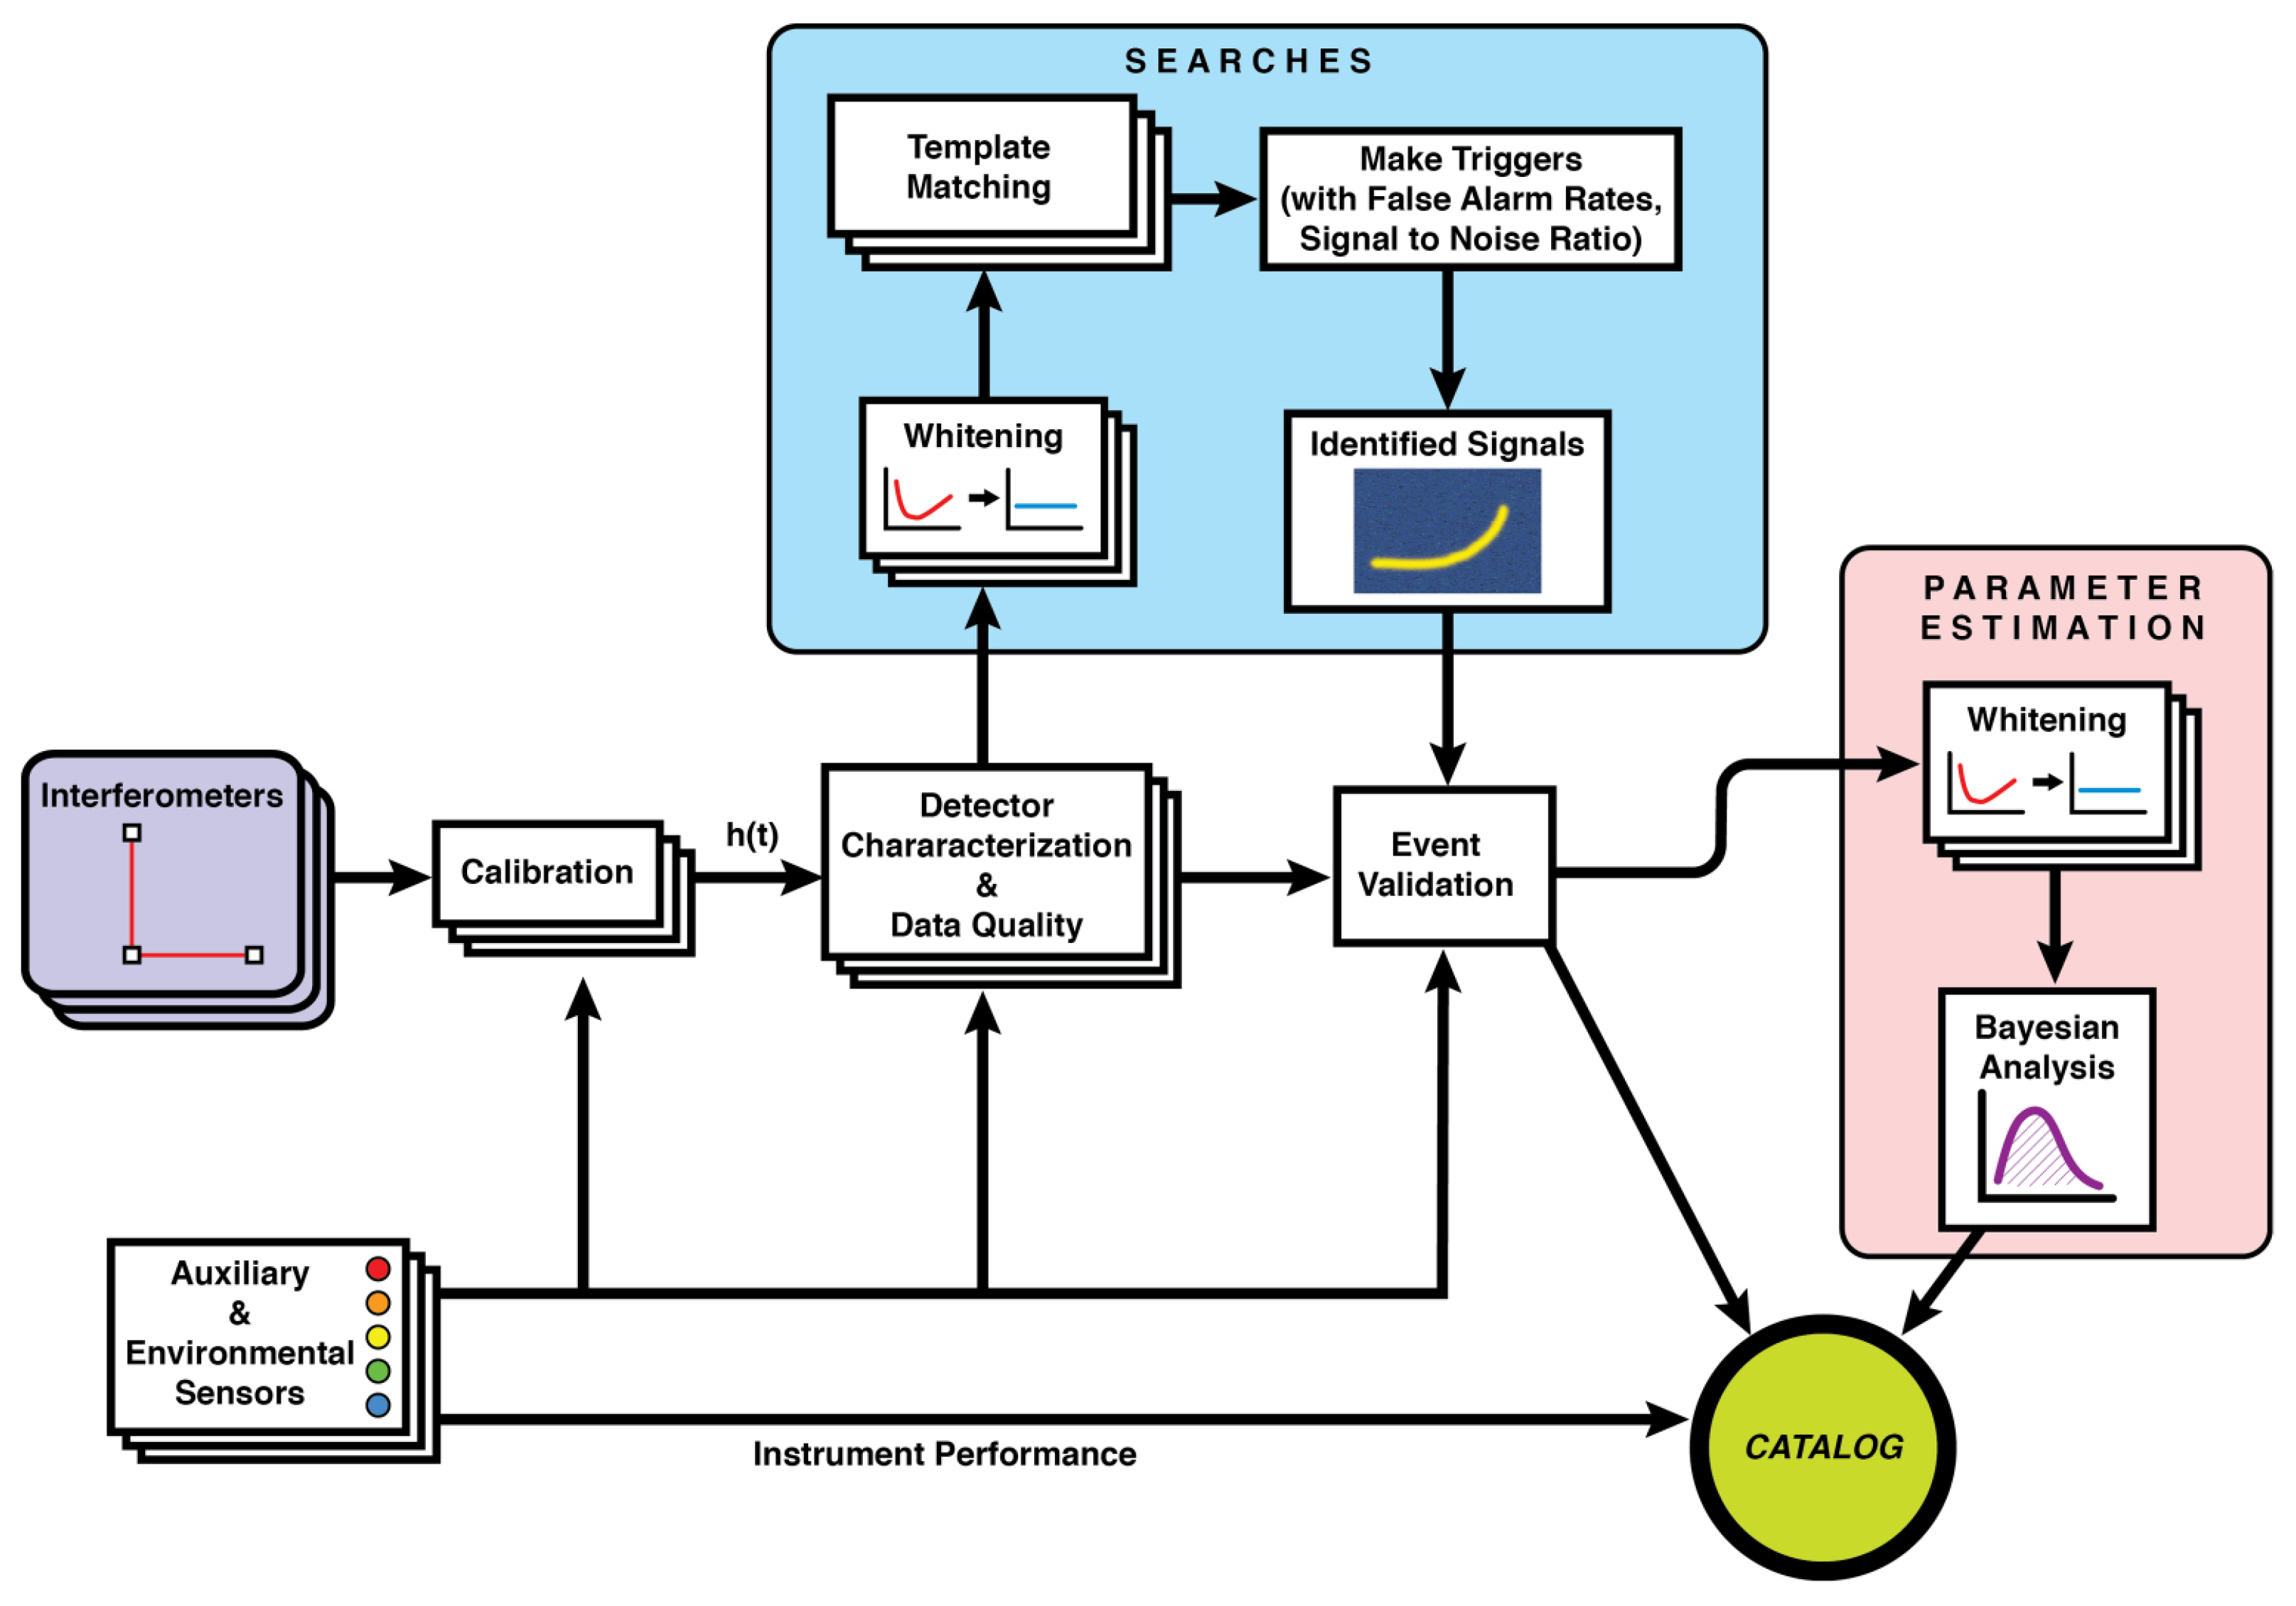
\includegraphics[width=0.98\textwidth]{figures/galaxies-10-00012-g001.png}
\caption{地面引力波数据分析与探测器表征的实际工作流示意。干涉仪数据经标定得到应变时间序列 $h(t)$，并与辅助通道、环境传感器和数据质量信息共同进入搜索、事件验证和参数估计流程；最终可靠候选事件进入引力波事件目录。图引自 Davis 与 Walker 对地面引力波探测器表征和噪声缓解工作的综述~\cite{Davis2022DetectorCharacterization}。}
\label{fig:pipeline}
\end{figure}

\begin{table}[htbp]
\centering
\caption{Advanced LIGO 主要噪声源特性对比}
\label{tab:noise_sources}
\small
\begin{tabular}{lcccc}
\hline
\textbf{噪声类型} & \textbf{主导频段} & \textbf{物理机制} & \textbf{降低方法} & \textbf{典型量级} \\
\hline
量子散粒噪声 & $\gtrsim 200$ Hz & 光子计数泊松涨落 & 提高激光功率、压缩光 & $4\times10^{-24}/\sqrt{\text{Hz}}$ \\
辐射压力噪声 & $\lesssim 50$ Hz & 光子动量涨落 & 增大镜面质量 & $10^{-23}/\sqrt{\text{Hz}}$ \\
热噪声（镜面） & 20--200 Hz & 布朗运动 & 低温、高Q材料 & $10^{-23}/\sqrt{\text{Hz}}$ \\
热噪声（悬挂） & 10--50 Hz & 悬丝热涨落 & 熔融石英纤维 & $10^{-23}/\sqrt{\text{Hz}}$ \\
地震噪声 & $\lesssim 10$ Hz & 地面振动 & 主动隔振系统 & $10^{-21}/\sqrt{\text{Hz}}$ \\
重力梯度噪声 & $\lesssim 10$ Hz & 引力直接耦合 & 地下建设、传感器减除 & $10^{-21}/\sqrt{\text{Hz}}$ \\
频谱线 & 离散频率 & 电源、机械共振 & 陷波滤波器 & 局部超出 $10\times$ \\
\hline
\end{tabular}
\end{table}

引力波数据预处理的每一步都有其不可忽视的物理动机，理解这些动机是正确实施预处理的关键。白化操作消除了噪声PSD的频率依赖性，使各频率分量的噪声贡献归一化——这一步骤对于深度学习方法尤为关键，因为神经网络如果直接处理非白化数据，其训练过程将被低频大噪声所主导，导致网络对低频引力波特征不敏感。带通滤波则利用了引力波信号频段的物理先验：引力波信号主要集中在探测器灵敏频段（地面探测器约20-1000 Hz），带通滤波在保留信号的同时去除灵敏频段以外的噪声成分，相当于在预处理层面已经利用了物理知识。Q变换的时频表示为机器学习方法提供了直观且信息丰富的输入格式：引力波的啁啾特征在Q变换时频图上表现为清晰的“上弯曲线”，这种直观特征既便于人工识别，也使CNN能够通过卷积操作高效提取。

从系统工程角度，数据预处理流水线的设计需要在物理严格性和计算效率之间取得平衡。对于在线（实时）引力波搜索，每一步预处理都必须在严格的时间约束下完成——通常要求整个预处理流水线在信号到达后1-2秒内完成，以便后续的触发判断和多信使预警。这一约束限制了预处理步骤的复杂程度：可以使用的噪声PSD估计窗口通常为4-256秒（而非更长时间的精确估计），白化滤波器的时域长度受限，Q变换的参数也需要在精度和速度之间折中。理解这些工程约束，对于在实际引力波数据分析流水线中部署AI方法时做出合理的设计选择，是不可缺少的背景知识。

引力波数据预处理方法本身也在持续发展中。传统的Welch方法（使用历史数据的段平均估计噪声PSD）在噪声平稳时表现良好，但在噪声突变时（如仪器状态改变后）需要一段时间才能重新收敛，导致过渡期内的白化质量下降。基于机器学习的噪声估计方法——如使用LSTM或Transformer追踪噪声PSD的时间演化——可以更快速地适应噪声变化，预计在下一代探测器（Einstein Telescope、Cosmic Explorer）的噪声管理中发挥重要作用。类似地，glitch的实时处理方法也在从“事后减除”向“实时抑制”演进：深度学习去噪方法（第7章）可以在数据产生后毫秒内完成glitch的识别和部分减除，为后续的匹配滤波提供更干净的输入数据。这种“AI预处理+经典分析”的流水线架构，是未来引力波数据分析基础设施的重要发展方向，也是物理-数据融合（第9章）在系统层面的具体体现。

噪声功率谱密度的精确估计对引力波参数估计的精度有直接影响。在贝叶斯参数估计中，引力波似然函数 $\ln p(d|\theta) = -\frac{1}{2}\langle d-h(\theta), d-h(\theta)\rangle$ 中的内积依赖于PSD作为噪声权重；若PSD估计存在偏差，则似然函数值将系统性偏离真实值，导致参数后验分布偏移。这一效应在低信噪比事件（$\rho < 12$）中尤为显著，因为PSD估计的相对误差与SNR成反比地影响后验的偏移量。LIGO标准分析流程使用BayesLine算法对每个候选事件进行精细的PSD估计，将PSD不确定度作为额外的贝叶斯自由度纳入参数估计框架，从而减轻PSD估计误差对参数精度的影响。深度学习方法在处理这一问题时具有独特优势：通过在训练数据中引入不同PSD条件的模拟，网络可以隐式地学习对PSD不确定性的鲁棒性，而无需显式地建模PSD不确定度——这是深度学习的“隐式正则化”特性在数据预处理环节的具体体现。

本章系统建立了引力波数据分析的物理与数学基础，为后续各章的方法介绍提供了完整的理论框架。

在引力波基本理论方面，从爱因斯坦场方程的线性化出发，推导了引力波的波动方程和 TT 规范下的极化描述，阐明了四极辐射公式和轨道衰减机制，并系统介绍了后牛顿展开的物理内容和频域 SPA 波形表示。啁啾质量作为引力波信号中测量最精确的参数组合，其主导地位来自后牛顿展开的最低阶项，是匹配滤波和参数估计的核心工具。

在引力波源类型方面，地面探测器对应的高频窗口与 LISA/太极/天琴覆盖的毫赫兹窗口共同构成了多模态信号空间。BBH 的质量分布复杂结构（约 $10\,M_\odot$ 和 $35\,M_\odot$ 处的峰值、质量间隙中的候选体）对黑洞形成机制提出了重要约束；GW170817 的多信使观测揭示了双中子星并合是短伽马射线暴和千新星的起源；EMRI 的精密相位演化是对 Kerr 时空几何的极精密测绘；随机引力波背景携带了宇宙早期历史的信息。空间探测器的多源叠加特性（数百万个信号同时存在）是全局拟合问题的根本来源。

在噪声建模方面，功率谱密度 $S_n(f)$ 是描述噪声频率特性的核心量，量子散粒噪声、热噪声和重力梯度噪声分别主导高频、中频和低频段。真实探测器的非高斯暂态（glitch）和非平稳漂移使高斯平稳假设在实践中受到严峻挑战，是引力波搜索中误报率的主要来源。标准量子极限（SQL）和量子压缩光技术代表了量子噪声控制的前沿，低温技术（KAGRA、ET）是降低热噪声的根本途径，地下建设是突破重力梯度噪声限制的必要选择。

在数学建模方面，标准内积定义、最优 SNR 公式和贝叶斯似然函数构成了后续所有方法的数学基础。Fisher 信息矩阵给出了参数估计精度的理论下界，揭示了参数简并的结构，是模板库设计的理论依据。白化操作建立了频域内积与时域 $L^2$ 内积的等价关系，是深度学习方法的必要预处理步骤。Q 变换提供了引力波信号的直观时频表示，数据质量控制和 glitch 处理是保证分析可靠性的重要环节。这些基础工具和概念将贯穿本书后续各章，是理解 AI 方法设计选择的物理基础。

\section{本章小结}

本章建立了引力波数据分析的物理与数学基础。在信号模型方面，TT规范下的度规扰动和天线响应函数描述了探测器的测量原理，IMRPhenomX和EOBNR等现象学波形模型覆盖了旋进-并合-衰荡的完整波形，构成模板库和参数估计的核心工具。在源类型方面，地面探测器对应的高频窗口与 LISA/太极/天琴覆盖的毫赫兹窗口构成了多模态信号空间，其中空间探测器的多源叠加特性是数据分析的核心挑战。在噪声建模方面，功率谱密度$S_n(f)$是描述噪声频率特性的核心量，而真实探测器的非高斯暂态（glitch）和非平稳漂移使高斯平稳假设在实践中受到严峻挑战。标准内积定义、最优SNR公式和贝叶斯似然函数构成了后续所有方法的数学基础，白化、带通滤波、Q变换等预处理步骤则是数据进入分析流程的必要前提。


%% ================================================================
%% 第二部：传统方法与局限
%% ================================================================
\foottheme{}
\footimage{figures/faraday.jpg}
\foottext{在高斯平稳噪声中，匹配滤波是最优的线性检测器——这是奈曼-皮尔逊引理的直接推论。\hfill —— 引力波数据分析经典结论}
\pagestyle{mystyle}

\part{经典方法及其可扩展性边界}

\renewcommand{\parttitle}{经典方法及其可扩展性边界}

\chapter{经典引力波数据分析方法}

在机器学习方法进入引力波数据分析领域之前，这一领域已发展出一套成熟且严格的经典方法体系。理解这一体系——其理论基础、实际性能、以及内在局限——是把握后续各章 AI 方法动机的前提。本章系统介绍匹配滤波、贝叶斯推断框架，以及这两类方法在实际引力波分析中的应用与挑战。

\section{匹配滤波与模板库构建}

匹配滤波（matched filtering）是引力波信号搜索的经典方法，其理论基础是奈曼-皮尔逊引理：在高斯平稳噪声中，匹配滤波给出最大信噪比，是最优的线性检测器~\cite{Allen2012PyCBC}。

给定探测器输出 $d(t) = h(t) + n(t)$，与模板 $\hat{h}(t;\theta)$ 的匹配滤波统计量（信噪比时间序列）为
\begin{equation}
  \rho(t;\theta) = \frac{\langle d, \hat{h}(\theta)\rangle}{\sqrt{\langle \hat{h}(\theta), \hat{h}(\theta)\rangle}},
\end{equation}
其中内积 $\langle a,b\rangle = 4\,\mathrm{Re}\int_0^\infty \tilde{a}(f)\tilde{b}^*(f)/S_n(f)\,\mathrm{d}f$。当 $\rho$ 超过预设阈值时触发候选事件。

模板库（template bank）的构建是匹配滤波的核心工程挑战。对双黑洞系统，质量参数空间需要用足够密集的模板覆盖，使任意真实信号与最近模板的匹配度（fitting factor）不低于 97\%。对于非旋转双黑洞，模板数量约为 $10^4$--$10^5$；加入自旋参数后，模板数量可增至 $10^6$--$10^7$。每个数据段需与所有模板做匹配滤波，计算量随模板数线性增长。

在实际搜索流水线（如 PyCBC、GstLAL）中，匹配滤波之后还需要一系列后处理步骤：$\chi^2$ 时频检验用于鉴别 glitch 产生的高信噪比触发；多探测器耦合检验要求两台或以上探测器在光速传播时延内同时触发；最终以误报率（false alarm rate，FAR）作为候选事件的显著性指标。

\subsection{PyCBC 与 GstLAL：实际搜索流水线}

PyCBC 和 GstLAL 是 LIGO-Virgo-KAGRA 合作组用于引力波搜索的两套主要流水线，均基于匹配滤波，但在实现细节和设计哲学上有所不同。

\textbf{PyCBC} 采用离线批处理模式，将数据分段（通常每段 256 秒）进行匹配滤波，然后在时间上合并触发事件~\cite{Usman2016PyCBCsearch,Nitz2021PyCBC}。其核心优势在于：基于 GPU 加速的高效 FFT 实现，使得对数百万条模板的并行匹配滤波在实践中可行；严格的 $\chi^2$ 时频检验，通过将信号频带分成若干子带分别计算 SNR，检验触发事件的时频一致性；以及基于背景估计的误报率计算，通过时间滑移（time slides）方法估计噪声背景的统计特性。

\textbf{GstLAL} 采用在线流处理模式，能够在数据产生后数秒内给出触发事件，适合低延迟预警场景~\cite{Messick2017GstLAL,Cannon2012GstLAL}。其核心技术是奇异值分解（SVD）模板压缩：通过对模板库进行 SVD 分解，将数千条模板压缩为少量正交基向量，大幅降低实时匹配滤波的计算量，同时保持与完整模板库相当的灵敏度。

两套流水线的结果通过 GWTC（引力波暂态目录）发布~\cite{Abbott2021GWTC3,Abac2025GWTC4}，构成了引力波天文学的核心数据产品。GWTC-3 系统汇总了 O1--O3 观测轮次的近百个引力波候选事件；随后 O4a 数据发布的 GWTC-4.0 进一步扩展了公开样本规模。O1 期间 PyCBC 和 GstLAL 对三个 BBH 事件（GW150914、GW151226、GW151012）的系统性分析~\cite{Abbott2016O1BBH}奠定了引力波天文学的方法论基础。

\subsection{匹配滤波的理论最优性与实践局限}

奈曼-皮尔逊引理保证了匹配滤波在高斯平稳噪声下的最优性，但这一最优性的背后是一系列严格的理论假设，值得深入分析。在信号假设检验的框架下，判断“信号存在”与“纯噪声”的最优判决来自似然比：
\begin{equation}
\Lambda = \frac{p(d|h)}{p(d|0)} = \exp\!\left(\langle d, h\rangle - \frac{1}{2}\langle h, h\rangle\right).
\end{equation}
最大化 $\Lambda$ 等价于最大化匹配滤波统计量 $\rho$，在高斯噪声且波形已知的假设下这是最优的线性检测器。然而“线性”这一约束本身值得关注——在非高斯噪声中，更优的检测统计量可能包含非线性成分；深度学习方法的端到端特性允许网络学习非线性的检测策略，这是其在真实噪声中相对于标准匹配滤波流程具有改进潜力的重要原因。

模板库的密度要求来自匹配度（fitting factor）的概念。任意真实信号 $h(\theta)$ 与模板库中最近模板 $h(\theta^*)$ 的匹配度定义为 $\mathcal{FF} = \max_{\theta^*}\mathcal{M}(h(\theta), h(\theta^*))$，其中 $\mathcal{M}$ 是归一化内积（match）。要求 $\mathcal{FF} \geq 0.97$ 意味着因模板不完备导致的SNR损失不超过3\%，对应体积损失约9\%（$1 - \mathcal{FF}^3 \approx 9\%$）。满足这一密度要求的模板数随参数空间维度快速增长：非旋转双黑洞（2维质量空间）需约 $10^4$ 条，加入对齐自旋（3维）需约 $10^5$ 条，加入进动效应（6维有效自旋维度）需约 $10^7$ 条。若试图以传统均匀模板库覆盖完整15维参数空间，计算代价将在当前资源条件下变得难以接受——这直接催生了对计算高效的人工智能方法的需求。

\subsection{$\chi^2$检验的物理原理与统计特性}

$\chi^2$时频检验是匹配滤波后处理中最重要的glitch鉴别工具，其物理思想极为深刻：一个真实的引力波信号在时频图上遵从特定的演化轨迹（啁啾特征），其贡献在各频率子带之间应该按照波形的功率谱分布均匀分配；而一个glitch（如blip或koi fish噪声）通常只在特定的频率区间产生高信噪比响应，其频率分布与引力波模板的分布不符。

具体地，将信号频带分为 $p$ 个等贡献子带（即每个子带对理想匹配信号的期望 SNR 贡献相同），每个子带分别计算匹配滤波响应。对于真实信号，各子带响应应与模板预期一致，构造出的 Allen $\chi^2$ 统计量近似服从自由度为 $2p-2$ 的 $\chi^2$ 分布；而由 glitch 产生的触发，其功率常集中在少数子带，导致 $\chi^2$ 值异常偏大。实践中通常使用约十几个子带，并将归一化后的 reduced-$\chi^2$ 与 SNR 组合为重加权 SNR，使真实信号的有效 SNR 基本保持，而 glitch 触发的排序统计量显著下降。

\subsection{时间滑移背景估计方法}

准确估计引力波搜索的误报率（FAR）是建立事件显著性的关键。引力波探测的误报来源于噪声涨落产生的偶然耦合：在两台探测器的数据中，分别出现高SNR触发，且两者在时间上落入允许的传播时延窗口（约 $\pm 10\,\mathrm{ms}$）。直接从理论计算这种偶然耦合率非常困难，因为需要准确描述噪声的统计分布（包括非高斯的glitch成分）。

时间滑移方法提供了一个有效的经验解决方案：将一台探测器的数据时间平移若干个离散步长（通常远大于探测器间光行时），与另一台探测器的原始数据重新计算耦合。由于真实天体信号只可能在约10 ms量级的传播时延内形成多探测器对应，较大的非物理时间平移会破坏真实信号的相干对应关系，使滑移样本可以近似表征噪声偶然耦合背景。通过大量时间滑移的统计，可以估计低误报率区域的噪声背景，从而对引力波事件候选体给出显著性评估。

O3期间PyCBC通过约200次时间滑移，生成了约200倍实际观测时长的背景数据，足以统计到FAR约 $1/10^4$ 年量级的稀有耦合事件，为近百个引力波事件候选体提供了可靠的显著性估计。

低延迟引力波预警与多信使天文学是匹配滤波方法在实际应用中的重要扩展方向。GW170817双中子星并合事件的成功多信使观测表明，在引力波事件后约1.7秒内探测到伽马射线暴（GRB 170817A），进而触发全球数十台电磁望远镜的联合后随观测，最终在距离事件约11小时后发现了千新星（kilonova）的光学对应体。低延迟流水线和 BAYESTAR 能够在分钟量级完成候选识别和快速天空定位计算，但 GW170817 的首个公开 GCN 警报由于数据质量处理和人工审核等原因在并合后约40分钟发布；这一经历恰恰说明，低延迟分析不仅取决于算法速度，还取决于数据质量控制、审核策略和预警分发机制。与此形成对比，如果完全依赖离线批处理的 MCMC 参数估计（需要数小时），则可能错过千新星早期光变曲线中最有价值的阶段。因此，低延迟引力波分析的计算速度不仅是技术效率问题，而是直接决定多信使科学产出的天文学关键因素。

深度学习信号识别方法的一个核心优势，正在于其毫秒级的在线推断速度：它有望把部分触发和初筛环节压缩至毫秒级，从而在未来更高事件率条件下分担低延迟预警管道的计算压力。这是第5章深度学习信号识别方法的核心动机之一，也是从“有没有”引力波信号到“更快知道”引力波信号这一转变的技术基础。

图~\ref{fig:mf_pipeline} 将上述步骤压缩为一个概念化流程。需要强调的是，图中的单探测器 SNR 阈值只表示触发生成阶段的初筛；真实事件的可信度来自重加权 SNR、$\chi^2$ 时频一致性、多探测器耦合、时间滑移背景、数据质量审查和候选事件验证的综合结果，而不是某一个阈值本身。

\begin{figure}[htbp]
\centering
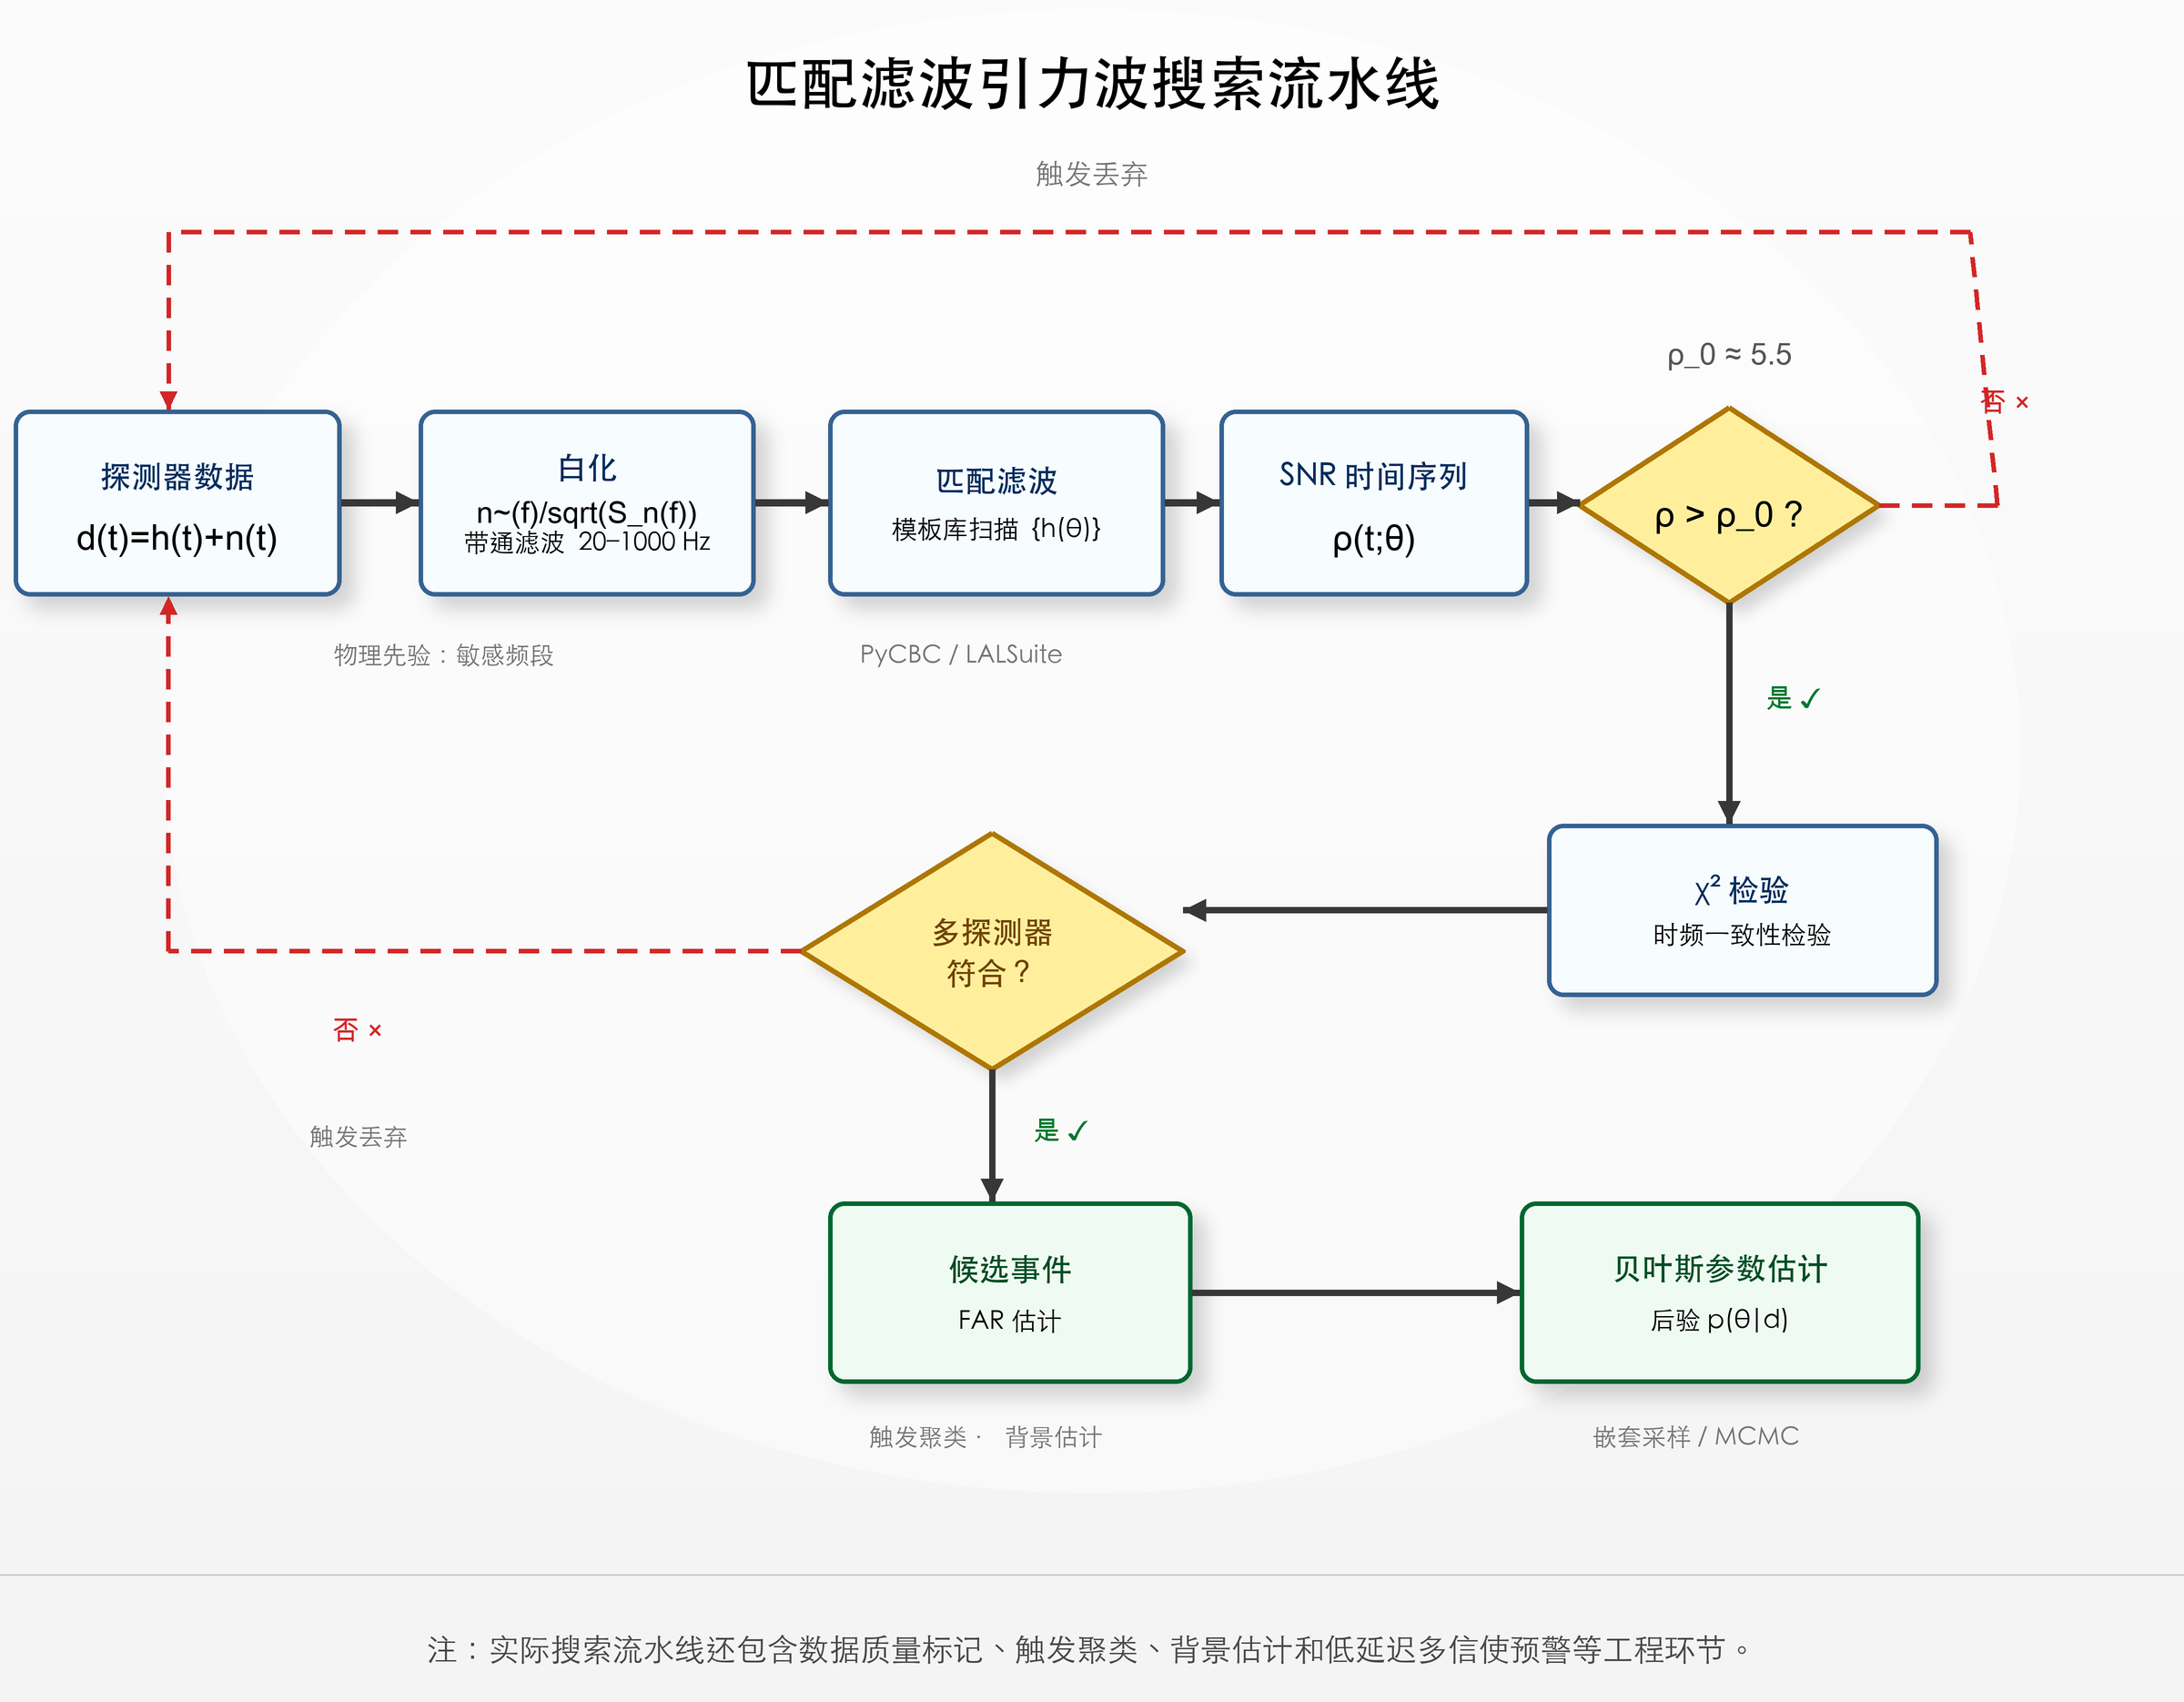
\includegraphics[width=0.98\textwidth]{figures/matched_filter_search_pipeline.png}
\caption{匹配滤波引力波搜索流水线概念图。探测器数据经白化与带通滤波后，与模板库逐一匹配生成 SNR 时间序列；超过触发阈值的候选触发还需通过 $\chi^2$ 时频一致性检验、多探测器耦合检验、触发聚类和背景估计，最终以 FAR 等统计量评估显著性，并进入贝叶斯参数估计。图中 $\rho_0 \approx 5.5$ 仅表示单探测器触发阈值的典型量级，实际搜索阈值和排序统计量随流水线、模板区域和数据质量状态而调整~\cite{Allen2012PyCBC,Usman2016PyCBCsearch,Nitz2021PyCBC,Messick2017GstLAL}。}
\label{fig:mf_pipeline}
\end{figure}

引力波数据分析主要在频域进行，这源于两个实际优势：其一，噪声的功率谱密度 $S_n(f)$ 在频域是对角化的（对于平稳噪声），使内积计算转化为简单的频域加权积分；其二，快速傅里叶变换（FFT）使频域计算在实践中高效可行。

时频域方法（Q 变换、短时傅里叶变换、小波变换）在特定场景下具有优势。对于短持续时间的信号（如双黑洞并合的并合-衰荡阶段）或未建模信号（如超新星核坍缩、宇宙弦碰撞），时频图能够直观显示信号的时频演化特征，是无模板搜索（burst search）的基础工具。Coherent WaveBurst（cWB）等算法~\cite{Klimenko2016cWB}在时频域寻找多探测器相干的超出噪声背景的能量聚集，不依赖于具体波形模板，对未建模信号更为敏感。

Q变换是引力波数据可视化的标准工具，其数学定义为：$X(t_0, f_0; Q) = \int d(t) w(t-t_0; f_0, Q) e^{-2\pi i f_0 t} dt$，其中窗函数 $w$ 是以 $f_0$ 为中心频率、Q因子控制时频分辨率权衡的高斯窗。不同Q值（通常Q=5至Q=50）对应不同的时频分辨率：低Q值适合捕捉短时高频特征（并合阶段），高Q值适合追踪频率缓慢变化的长时信号（旋进阶段）。在GW150914的时频图上，Q变换清晰地显示了频率从35Hz到150Hz的啁啾轨迹，成为引力波探测历史上最具视觉冲击力的科学图像之一。

频域方法的计算优势体现在FFT的 $O(N\log N)$ 复杂度上，相比直接时域匹配（朴素实现约为 $O(N^2)$）有数个量级的加速。对于LIGO典型的采样率（16384 Hz）和数据段长度（256秒，即约400万采样点），现代 CPU/GPU 实现可以在很短时间内完成 FFT；而朴素时域卷积会随数据长度迅速变得昂贵。这一复杂度差异，是对大量模板进行批量扫描的计算基础。

小波变换在引力波数据分析中具有特殊地位，因为它在时域和频域之间提供了一种自适应的分辨率权衡。离散小波变换（DWT）将信号分解为一系列具有不同时频分辨率的子带，低频子带具有高频率分辨率但低时间分辨率，高频子带则相反。对于引力波信号，这一多尺度分解能够在低频旋进阶段（需要高频率分辨率）和高频并合阶段（需要高时间分辨率）之间自动分配合适的分辨率资源，优于固定分辨率的短时傅里叶变换。BayesWave算法~\cite{Cornish2015BayesWave}将小波基展开与贝叶斯框架结合，通过自适应选择小波个数和参数来描述引力波信号或噪声glitch，在未建模信号重建和glitch减除中取得了显著成效。

频域方法与时频域方法的互补性体现在实际分析流水线的设计中。现代引力波数据分析通常采用“频域主、时频辅”的双轨策略：主搜索使用匹配滤波（频域），充分利用波形模板的先验知识达到最优灵敏度；辅助搜索使用cWB或BayesWave（时频域），在不依赖精确模板的前提下探测可能超出模板库的信号，并对候选事件进行独立验证。两类方法的结果交叉比对，既提升了对已知类型信号的置信度，也保留了发现未知类型信号的可能性。这种方法论上的多样性，是引力波天文学保持科学严谨性的重要设计原则。

在噪声减除（noise subtraction）应用中，时频域方法展现出独特优势。部分LIGO噪声源（如散射光噪声、悬挂系统振动）具有已知的时频特征，可以通过频域陷波滤波器（notch filter）或时频域小波减除从数据中移除。然而，当噪声的时频形态与引力波信号存在部分重叠时，单纯的滤波会损失信号信息，需要更精细的建模方法。这一挑战催生了第7章讨论的深度学习去噪方法——通过学习噪声和信号的统计特性，在去除噪声的同时最大程度保留信号。

时频域表示作为深度学习方法的输入，在引力波机器学习研究中具有特殊的地位。相比原始时域数据，时频图（Q变换图）能够直观地展示引力波信号的啁啾特征，使卷积神经网络更容易学习信号的判别特征。从信息论角度，时频表示是原始数据的一种冗余变换（时域和时频域携带相同的信息量），但这种冗余变换对CNN而言具有实践优势：信号的啁啾轨迹在时频图中呈现为连续的“弧线”，这种局部连续的几何结构恰好适合CNN的局部感受野和权重共享机制。相比之下，原始时域数据中的啁啾特征是非局部的（早期旋进和晚期并合都贡献），需要更深的CNN才能建立长程依赖。因此，时频图输入 + 浅层CNN往往与时域输入 + 深层CNN（或Transformer）在性能上可比，但前者更易训练和解释。

\section{贝叶斯推断与参数估计框架}

一旦候选引力波事件被识别，参数估计的任务是推断波源物理参数 $\theta$ 的后验分布 $p(\theta|d)$~\cite{Christensen2022noise}。贝叶斯定理给出
\begin{equation}
  p(\theta|d) = \frac{p(d|\theta)\,p(\theta)}{p(d)},
\end{equation}
其中似然函数
\begin{equation}
  \ln p(d|\theta) = -\frac{1}{2}\langle d - h(\theta),\,d - h(\theta)\rangle
\end{equation}
需要对每个参数点生成理论波形 $h(\theta)$ 并与数据做内积运算，先验 $p(\theta)$ 编码了参数的先验知识（如质量范围、自旋幅度的物理约束），证据 $p(d) = \int p(d|\theta)p(\theta)\,\mathrm{d}\theta$ 用于模型比较（贝叶斯因子）。

双黑洞系统的参数空间通常为 15 维：两个分量质量 $(m_1, m_2)$、六个自旋分量 $(\vec{S}_1, \vec{S}_2)$、光度距离 $d_L$、天空位置 $(\alpha, \delta)$、轨道倾角 $\iota$、极化角 $\psi$、并合时刻 $t_c$、参考相位 $\phi_0$。后验分布通常是非高斯的，包含多个极大值（如天空位置的简并）和非对称的尾部。

用于引力波参数估计的标准软件工具包括 LALInference~\cite{Veitch2015LALInference}（基于 MCMC 和嵌套采样）和 Bilby~\cite{Ashton2019Bilby}（更模块化的贝叶斯推断框架），均已在 LIGO-Virgo 合作组的公开数据分析中广泛应用。嵌套采样算法~\cite{Skilling2006nested}是计算贝叶斯证据的标准方法，也是 LALInference 和 Bilby 的核心采样引擎之一。

引力波参数估计的科学产出不仅是参数的点估计，而是完整的后验概率分布 $p(\theta|d)$。后验分布包含了观测数据对物理参数约束的全部统计信息：其众数（mode）给出最可能参数值，其置信区间（credible interval）量化参数的不确定度，其形状（单峰/多峰、对称/不对称）揭示了参数之间的相关性和简并结构。LIGO-Virgo合作组发布的引力波事件参数估计结果（PE样本）是公开数据产品的重要组成部分，被大量后续天体物理和宇宙学研究用作输入数据。

引力波似然函数的结构对参数估计算法的设计有深刻影响。展开内积得到：$\ln p(d|\theta) = \langle d, h(\theta)\rangle - \frac{1}{2}\langle h(\theta), h(\theta)\rangle + \text{const}$。第一项是匹配滤波统计量，在已知噪声PSD的情况下通过FFT高效计算（$O(N\log N)$）；第二项是模板自相关，仅依赖于模板参数，可以预计算并缓存，避免在MCMC每步重复计算。这一分解使得似然函数的实际计算代价约等于单次波形生成的代价——毫秒量级（后牛顿模型）到秒量级（精确数值相对论波形），是决定参数估计总计算时间的主要因素。

\subsection{贝叶斯因子与模型比较}

贝叶斯框架不仅用于参数估计，还用于模型比较。两个竞争模型 $\mathcal{H}_1$（信号+噪声）和 $\mathcal{H}_0$（纯噪声）之间的贝叶斯因子为
\begin{equation}
  \mathcal{B}_{10} = \frac{p(d|\mathcal{H}_1)}{p(d|\mathcal{H}_0)} = \frac{\int p(d|\theta,\mathcal{H}_1)p(\theta|\mathcal{H}_1)\,\mathrm{d}\theta}{p(d|\mathcal{H}_0)},
\end{equation}
其中分子为信号模型的贝叶斯证据，分母为噪声模型的证据。$\mathcal{B}_{10} \gg 1$ 表明数据强烈支持信号假设。

贝叶斯因子在引力波天文学中有多种应用：检验广义相对论（比较 GR 波形与修正引力理论波形的证据）、判断信号是否包含进动效应或高阶模式、以及评估候选事件的天体物理起源。嵌套采样算法（MultiNest、dynesty）在计算后验分布的同时自然给出贝叶斯证据，是引力波模型比较的标准工具。

引力波贝叶斯模型比较的一个重要应用是检验双黑洞系统是否存在自旋进动效应。在准圆轨道双黑洞系统中，若两个黑洞的自旋方向与轨道角动量方向不一致（即非对齐自旋），则自旋-轨道耦合将导致轨道平面进动，引力波极化模式随之发生特征性的调制。检验进动的贝叶斯因子 $\mathcal{B}_\mathrm{prec}$ 定义为进动波形模型证据与非进动波形模型证据之比，$\mathcal{B}_\mathrm{prec} > 1$ 表明数据支持进动假设。在GWTC-3的系统性分析中，多数事件的 $\mathcal{B}_\mathrm{prec}$ 接近于1（约0.5--2），表明当前数据质量不足以区分进动与非进动情形；少数事件（如GW200129）曾显示出进动证据，但其显著性和对噪声建模的依赖仍是后续研究讨论的重点。

高阶多极模式（higher-order multipole modes，HOM）的检测是另一类重要的模型比较应用。在后牛顿框架下，引力波辐射由多个多极矩共同贡献，主导项为 $\ell=2, m=\pm2$ 的四极模式，高阶项（$\ell=2,m=1$；$\ell=3,m=3$；$\ell=4,m=4$ 等）贡献通常较小。对于质量比接近1的对称系统，高阶模式幅度很小；对于质量不对称系统（$q = m_2/m_1 \ll 1$）或大倾角观测，高阶模式贡献显著增强。GW190814（质量比约0.11）和GW190412（质量比约0.28）是高阶模式证据较强的代表性事件；这些结果说明，在不对称质量比或有利观测几何的事件中，将高阶模式波形模型纳入分析十分必要。

\subsection{参数简并与先验选择}

引力波参数估计中存在多种参数简并，对后验分布的形状有重要影响。

\textbf{质量简并}：对于低信噪比事件，啁啾质量 $\mathcal{M}$ 测量精确，但质量比 $q = m_2/m_1$ 的约束较弱，导致后验分布在 $(m_1, m_2)$ 平面上沿等 $\mathcal{M}$ 曲线延伸。

\textbf{天空位置简并}：对于两台探测器的观测，天空位置后验分布通常呈现两个对称的环形区域（对应两个可能的到达方向），加入第三台探测器（Virgo）后可以打破这一简并。

\textbf{距离-倾角简并}：光度距离 $d_L$ 和轨道倾角 $\iota$ 对引力波幅度的影响存在简并，导致两者的联合后验分布呈现强相关性。

先验分布的选择对后验结果有显著影响，尤其在信噪比较低时。标准先验通常选择：质量在物理范围内均匀分布、自旋幅度均匀分布、天空位置各向同性、距离按 $d_L^2$ 分布（对应均匀体积密度）。这些先验选择反映了对引力波源分布的天体物理假设，在解释参数估计结果时需要明确说明。

引力波参数估计的科学产出不仅是参数的点估计，而是完整的后验概率分布。后验分布的形状本身携带了丰富的物理信息：尖锐的单峰分布意味着参数被精确约束（如啁啾质量），宽泛的多模态分布意味着数据不足以区分不同的参数组合（如天空位置在两台探测器配置下的双环结构）。LIGO-Virgo合作组发布的引力波事件参数估计结果（PE样本）是公开数据产品的重要组成部分，包含了后验分布的完整Monte Carlo样本，被大量后续天体物理和宇宙学研究直接使用。对于GW150914，其参数后验样本包含约10万个独立样本，每个样本对应一组完整的15维参数值，研究者可以从这些样本直接计算任意参数组合的边缘后验分布或联合后验分布（如 $m_1$-$m_2$ 联合分布、$d_L$-$\iota$ 距离-倾角联合分布）而无需重新运行参数估计。

先验分布的选择是引力波参数估计的重要方法论议题，对结果的解释有深刻影响。对于质量参数，标准选择是分量质量的均匀先验（$p(m_1,m_2) \propto 1$，在物理允许范围内）；但若改用啁啾质量均匀先验，则对不同质量比系统的权重不同，会改变质量比的边缘后验形状。对于自旋参数，标准选择是自旋幅度均匀分布于 $[0,1]$，方向在球面上各向同性；这对应“不了解自旋大小和方向”的最小信息先验。然而，若对双黑洞形成机制有先验知识（如孤立双星演化倾向于对齐自旋），则可以使用更具信息性的先验，但这会将物理模型假设引入参数估计，需要明确说明和检验。在GWTC-3的分析中，LIGO合作组系统研究了不同先验选择对参数估计结果的影响，发现对大多数参数先验选择的影响不超过后验不确定度的10\%，但对于信噪比较低（$\rho < 10$）的事件，先验影响可达30\%以上，此时需要格外谨慎地报告和解释结果。

LALInference 和 Bilby 是引力波参数估计的两套主要软件框架。LALInference 是 LVK 合作组长期使用的分析软件，基于 C/Python 混合实现，包含多种 MCMC 变体（适应性 MCMC、并行回火 MCMC）和嵌套采样（MultiNest、Nested sampler），已在 O1-O3 的公开分析中广泛使用。Bilby 是更近期的模块化 Python 框架，设计目标是提高用户友好性和可扩展性，支持快速切换不同的采样器（dynesty、Nessai 等）和波形近似（IMRPhenomX、SEOBNRv4 等），是学术研究和 SBI 方法验证的常用平台。两者的结果在标准引力波事件上高度一致（后验分布在统计误差内相同），验证了不同实现方式的鲁棒性。

高维贝叶斯后验的数值计算是经典方法的核心计算瓶颈。两类主流采样方法各有优劣。

\textbf{马尔可夫链蒙特卡洛（MCMC）}：通过构造满足细致平衡条件的马尔可夫链，从目标分布中生成样本。适用于任意复杂的后验形状，但在高维多模态分布中混合效率低，收敛判断困难。对地面双黑洞事件，MCMC 参数估计通常需要数小时至数天。

\textbf{嵌套采样（Nested Sampling）}：同时估计证据和后验，通过逐步淘汰低似然区域的“活点”来探索参数空间。MultiNest 和 dynesty 是引力波参数估计中最常用的嵌套采样实现，收敛速度通常优于 MCMC，且自然给出贝叶斯证据用于模型比较。

两类方法的共同瓶颈在于：每次似然评估需要生成一条波形，对地面探测器的双黑洞系统约需毫秒量级，总计数百万次评估；对空间探测器的 EMRI 系统，单次波形生成可能需要数秒至分钟，使直接 MCMC/嵌套采样在现实计算预算下难以承担。

\textbf{并行回火（Parallel Tempering）}是解决多模态后验的重要技术。标准MCMC在多模态后验中极易陷入局部极值，因为跨越极值之间的低似然“势垒”需要极低概率的接受步骤。并行回火同时运行多条温度不同的链（温度从1到某个最大值），高温链在“热化”的后验 $p_T(\theta) \propto p(\theta|d)^{1/T}$ 上运行，势垒被有效降低，便于跨越；链之间定期交换配置（满足细致平衡条件），将高温链探索到的新极值引入低温（$T=1$）链。这一技术在引力波参数估计中已被广泛采用，特别是对于具有双峰天空位置后验的事件，并行回火可以确保两个峰值都被充分采样，给出正确的后验分布。

\textbf{哈密顿蒙特卡洛（HMC）}及其无调整版本NUTS（No-U-Turn Sampler）是另一类高效的MCMC变体。HMC利用目标分布的梯度信息引导采样，通过模拟辅助动量空间中的哈密顿动力学产生相关性更低的样本，特别适合高维连续参数空间。在引力波参数估计中，HMC/NUTS已被集成到Bilby框架中，对于后验分布较为规则（无严重多模态）的事件，其效率比标准Metropolis-Hastings算法高约10-100倍，将单事件参数估计时间从数天压缩至数小时。

嵌套采样（Nested Sampling）的工作原理是在似然函数的等高线之间系统地积分后验分布。算法维护 $N_\mathrm{live}$ 个“活点”（live points），均匀分布在似然大于当前阈值 $\mathcal{L}_i$ 的参数空间中；每步将最低似然活点替换为一个新的、似然更高的样本，被替换的活点作为“死点”贡献于后验分布的近似；通过递推关系 $Z = \sum_i w_i \mathcal{L}_i$（$w_i$ 是统计权重）估计证据。嵌套采样的优点在于自然输出贝叶斯证据（用于模型比较），且对多模态后验有较好的处理能力——只要活点数足够多，不同模态都能被充分覆盖。dynesty实现了动态嵌套采样，根据后验分布的局部形状自适应调整活点数，进一步提高了计算效率。

重要性采样（importance sampling）是另一种有价值的后验近似技术，在引力波参数估计中被用于快速修正近似波形模型的后验偏差。基本思路是：先使用计算快速但精度较低的波形模型（如PN波形）运行MCMC，获得近似后验分布 $q(\theta)$；再通过重要性权重 $w_i = p(d|\theta_i, h_\mathrm{exact})/p(d|\theta_i, h_\mathrm{approx})$ 对样本重新加权，得到基于精确波形模型的后验近似 $p(\theta|d)$。这一流程将计算代价最高的精确波形评估次数从 $\sim 10^7$（全MCMC运行）压缩至 $\sim 10^4$（仅对已有样本重加权），实现约1000倍的加速。然而，重要性采样的有效性依赖于近似后验 $q(\theta)$ 与真实后验 $p(\theta|d)$ 足够接近（否则权重方差爆炸，有效样本量 $\mathrm{ESS} = (\sum w_i)^2/\sum w_i^2$ 趋向于1）。对于参数估计精度要求不高或SNR较低的事件，这一近似可以接受；对于高SNR事件（如GW170817），两种波形模型的差异可能使重要性权重发生数量级的变化，需要更精确的近似出发点。

MCMC 方法的一个实践难题是收敛判断：如何确认马尔可夫链已经充分探索了目标分布，而非陷入局部区域？常用的收敛诊断方法包括：

\textbf{Gelman-Rubin 统计量}（$\hat{R}$）：运行多条独立链，比较链内方差与链间方差之比。$\hat{R} \approx 1$ 表明各链已收敛到相同分布；$\hat{R} > 1.1$ 通常被视为未收敛的警告信号。

\textbf{有效样本量}（ESS）：由于 MCMC 样本之间存在自相关，有效独立样本数少于总样本数。ESS 定量描述了这一损失：$\mathrm{ESS} = N / (1 + 2\sum_{k=1}^\infty \rho_k)$，其中 $\rho_k$ 为滞后 $k$ 的自相关系数。对于引力波参数估计，通常要求每个参数的 ESS 不低于数千。

\textbf{迹图检验}：直接观察参数值随 MCMC 步数的变化，检查是否存在明显的漂移或卡顿。这是最直观但也最主观的诊断方法。

在高维多模态后验（如 EMRI 的 17 维参数空间）中，上述诊断方法的可靠性大幅下降：链可能在局部极值附近收敛，给出虚假的“收敛”信号，而实际上未能探索到其他后验极大值区域。这是传统 MCMC 在 EMRI 参数估计中面临严重可扩展性困难的深层原因之一。

自适应MCMC是解决高维参数空间采样效率问题的重要改进。标准Metropolis-Hastings算法使用固定的提议分布（如各向同性高斯）来生成候选点，在高维空间中这往往导致接受率极低（$<5\%$）或极高（$>90\%$），两者都意味着低效的探索。自适应MCMC通过在线学习参数的协方差结构来调整提议分布：以历史样本估计后验的协方差矩阵，用其椭球形高斯作为提议分布，使提议方向与后验的高概率区域对齐。对于引力波参数估计，自适应MCMC通常能在约1000步预热后显著改善混合效率，将接受率维持在最优的约23\%（在高维情形下理论最优接受率）。LALInference的默认MCMC实现包含自适应提议和差分进化提议（differential evolution proposal），后者通过在两个当前链的样本之间插值生成提议，能够高效地沿后验的主方向探索。

引力波参数估计中的采样挑战，不仅来自参数空间的高维性，还来自后验分布的复杂形状。典型的双黑洞参数后验包含多种非高斯特征：天空位置呈环状（双探测器配置）或椭圆形（三探测器配置），距离-倾角联合后验呈香蕉形（由于正负倾角之间的简并），自旋参数后验呈蝴蝶结形（由于自旋方向关于轨道平面的反射对称性）。这些形状复杂性使得单一椭球形提议分布的自适应MCMC效率有限，需要更复杂的采样策略。在实际应用中，LALInference和Bilby采用了多种先进采样技术：对于多模态天空位置后验，使用天空定位的专用参数变换将环状后验转换为更规则的形状；对于高自旋参数的强相关后验，使用哈密顿蒙特卡洛（HMC）或NUTS采样器，利用梯度信息指导采样方向。这些技术细节的理解，有助于正确评估经典参数估计方法的当前能力边界，以及AI方法（特别是SBI）在突破这一边界上的具体贡献。

差分进化MCMC（DE-MCMC）是专为高维多峰后验设计的方法，在引力波参数估计中被广泛采用。标准差分进化通过在种群成员之间进行随机差分来生成新候选点：对于当前点 $\theta$，选取两个其他种群成员 $a$ 和 $b$，提议 $\theta' = \theta + F(a-b)$，其中 $F$ 是步长缩放因子（通常取 $F=2.38/\sqrt{2d}$，$d$ 为维度，来自高斯分布的最优步长理论）。这一提议机制自动适应后验的协方差结构（因为差分 $a-b$ 的方向与后验高概率区域的轴向对齐），且不需要显式估计协方差矩阵。对于引力波参数估计，DE-MCMC通常在约10000步内实现良好混合，接受率约为25\%，优于标准自适应MCMC约2-3倍。DE-MCMC的另一优点在于其天然的种群结构使得多模态后验的探索更为充分：当种群中部分成员已到达某一极值区域时，差分提议会以一定概率将其他成员拉向该区域，从而帮助整体种群跨越极值之间的低概率屏障。

\subsection{嵌套采样算法与MultiNest/dynesty实现}

嵌套采样（Nested Sampling）由Skilling于2004年提出~\cite{Skilling2004nested}，是引力波参数估计领域最重要的采样算法之一。其核心思想是通过引入先验质量变量 $X(\lambda) = \int_{p(d|\theta)>\lambda} p(\theta)\,\mathrm{d}\theta$，将高维贝叶斯证据积分
\begin{equation}
  \mathcal{Z} = \int p(d|\theta)\,p(\theta)\,\mathrm{d}\theta = \int_0^1 \mathcal{L}(X)\,\mathrm{d}X
\end{equation}
转化为一维积分，从而绕开在高维参数空间中直接计算证据积分的困难。

算法维护 $N_\mathrm{live}$ 个活跃点，每步移除似然最低的点并采样新的满足约束的点，逐步收缩至高似然区域，同时积累证据估计。嵌套采样的一个核心优势是在探索后验分布的同时自然输出贝叶斯证据，使其成为引力波模型比较（贝叶斯因子计算）的标准工具。

\textbf{MultiNest}~\cite{Feroz2009MultiNest} 是嵌套采样在引力波参数估计中应用最广泛的实现。其核心创新在于椭球采样策略：用多个椭球体近似当前活跃点所占据的参数空间区域，并通过多椭球分解（multi-ellipsoidal decomposition）处理多模态后验。对于标准双黑洞事件（15维参数空间），使用 $N_\mathrm{live} = 2000$ 的MultiNest通常需要约 $10^6$--$10^7$ 次似然评估，在32--128核MPI并行下墙钟时间约6--24小时。

\textbf{dynesty}~\cite{Speagle2020dynesty} 引入了动态嵌套采样框架，根据后验分布的局部形状自适应地调整活跃点数量，在后验复杂情形下比固定活跃点的MultiNest节省约30\%--50\%的计算时间。在Bilby框架中，dynesty是默认采样器~\cite{Ashton2019Bilby}，与GWTC-3分析中LALInference+MultiNest的结果高度一致（后验分布在统计误差内相同），验证了两套实现的鲁棒性。

嵌套采样的计算代价主要由波形生成时间决定：后牛顿波形（~0.1 ms/次）对应约0.5--5小时的参数估计，EOB波形（~10--100 ms/次）对应约10--60小时，而EMRI波形（~1--100 s/次）会使完整嵌套采样的墙钟时间达到数月量级，在常规分析流程中难以承受，这是第6章SBI方法的核心动机之一。

\subsubsection*{嵌套采样的局限性与SBI方法的互补关系}

尽管嵌套采样在引力波参数估计中取得了巨大成功，其固有局限性在面向未来任务时变得日益突出。

\textbf{高维参数空间的效率下降}是嵌套采样最主要的局限之一。随着参数维度 $d$ 的增加，约束先验区域（似然超过当前阈值的区域）在参数空间中的形状变得越来越复杂，椭球近似的质量迅速下降。理论分析表明，在 $d$ 维参数空间中，嵌套采样所需的活跃点数往往随维度快速增长，才能保持相同的后验采样精度。这使得 EMRI 的17维强简并参数空间，以及空间探测器全局拟合的高维参数空间，对直接嵌套采样提出了极高的计算要求。

\textbf{多模态后验的遗漏风险}是另一个重要局限。尽管MultiNest的多椭球分解策略在处理中等程度的多模态后验时表现良好，但对于极端多模态情形（如EMRI参数空间中约 $10^5$ 个似然极大值），任何有限数量的活跃点都无法保证覆盖所有模态。当活跃点数不足时，算法可能在早期迭代中就将某些模态所在的参数空间区域排除在外，导致后验估计系统性地遗漏重要的极大值。这种遗漏不会在算法的收敛诊断中显现（算法仍然“收敛”，只是收敛到了不完整的后验），是嵌套采样在复杂多模态问题中最危险的失效模式。

\textbf{重复运行的计算代价}是嵌套采样在实际应用中的另一个实践局限。对于每个新的引力波事件，嵌套采样都需要从头开始运行，无法利用之前事件的计算结果。在O3期间，LIGO-Virgo合作组对近百个引力波事件分别运行了完整的嵌套采样参数估计，总计算代价约为数百万CPU小时。随着未来探测器灵敏度的提升和事件率的增加，这一“每事件独立运行”的模式将变得难以为继。

上述局限性与基于模拟的推断（SBI）方法形成了鲜明的互补关系。SBI方法（第6章）通过训练神经网络来近似后验分布，将计算代价从“每事件 $10^6$--$10^7$ 次似然评估”转移到“一次性训练 $10^6$--$10^8$ 次模拟”，训练完成后对新事件的推断仅需毫秒量级的神经网络前向传播。这一范式转变使SBI在高事件率场景下具有显著的计算优势：训练代价被摊薄到大量事件上，单事件推断代价接近神经网络前向传播的成本。然而，SBI的近似性（神经网络对后验的近似误差）和对训练分布的依赖性（在训练分布之外的泛化能力有限），使其不能简单替代嵌套采样在精确参数估计和模型比较中的地位。

在实际引力波数据分析中，嵌套采样与SBI的组合策略正在成为研究热点：使用SBI进行快速初步参数估计，识别后验分布的主要结构；再使用嵌套采样在SBI确定的高概率区域内进行精细采样，获得精确的后验分布和贝叶斯证据。这种“粗筛+精算”的两阶段策略，有望将单事件参数估计的总时间从数十小时压缩至数小时，同时保持与纯嵌套采样相当的精度。其具体收益取决于SBI近似是否覆盖真实后验高概率区域、先验压缩策略是否保守以及后续采样是否充分。这一方向的探索，代表了经典方法与AI方法深度融合的重要前沿，也是第9章“物理驱动与数据驱动融合方法”的核心议题之一。

\section{经典方法的实际应用与局限}

\begin{figure}[htbp]
\centering
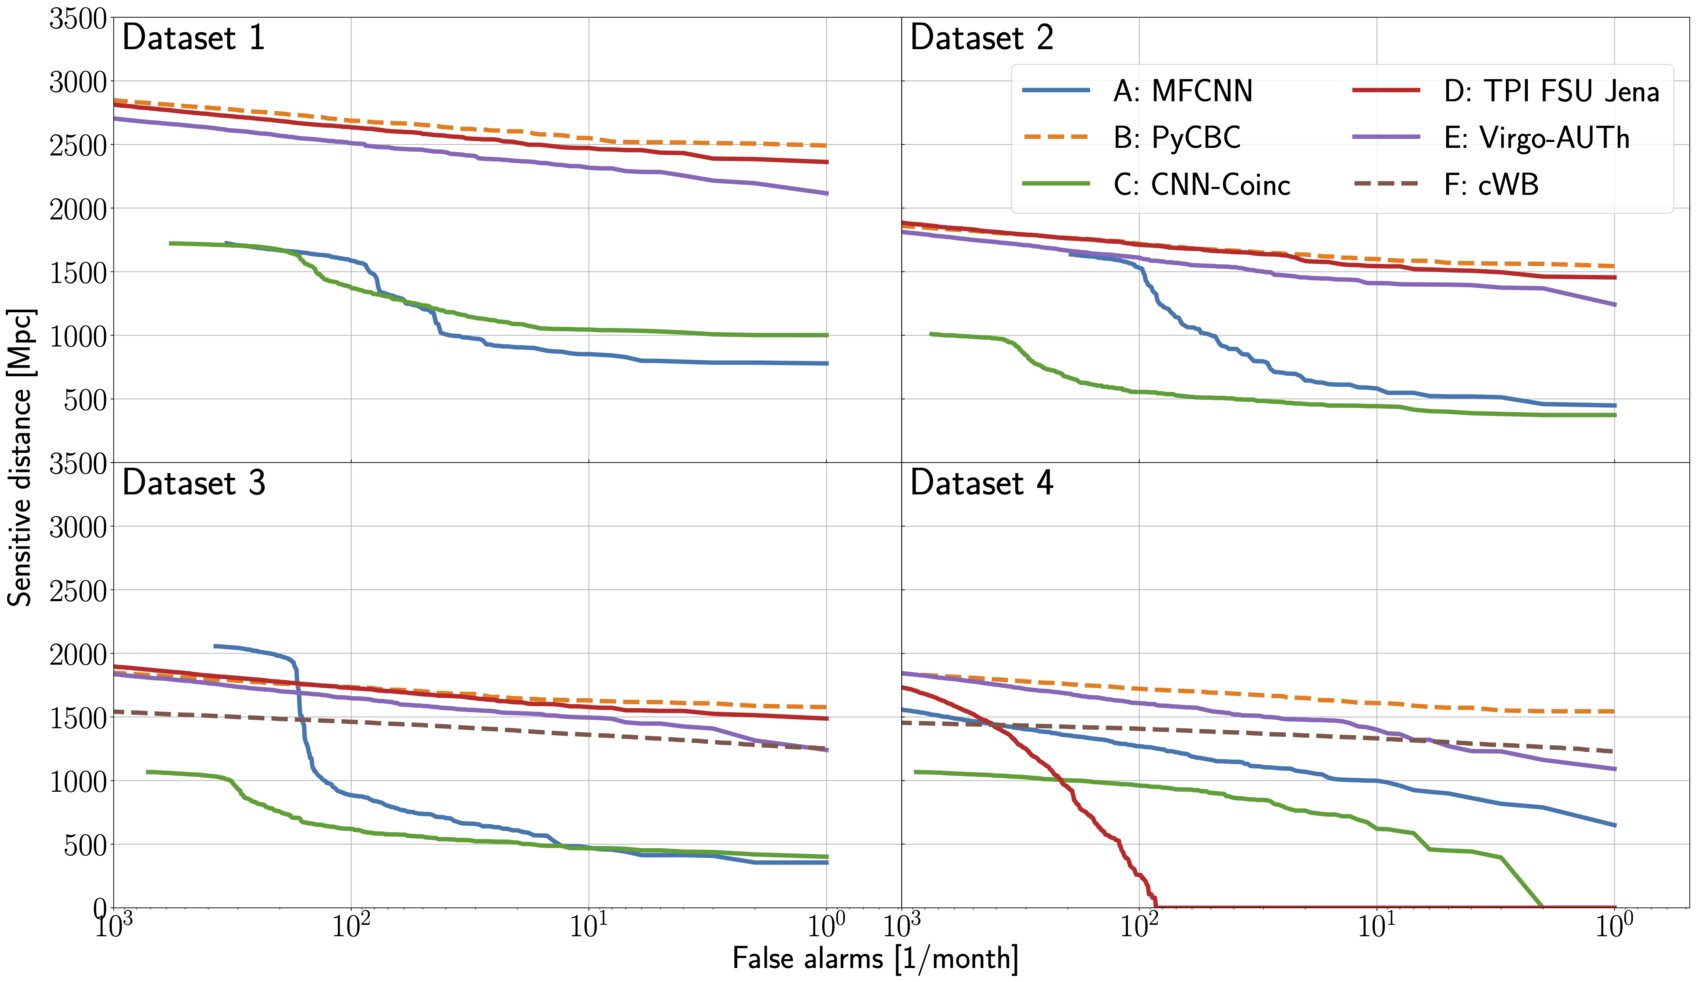
\includegraphics[width=0.98\textwidth]{figures/mlgwsc1_sensitive_distance.jpg}
\caption{MLGWSC-1 中各参赛搜索方法在四个数据集上的敏感距离随误报率变化曲线。横轴为误报率（false-alarm rate，FAR；单位为每月误报次数），纵轴为敏感距离（Mpc）；实线表示以机器学习为核心的搜索方法，虚线表示非机器学习基线。四个数据集的复杂度逐级提高，Dataset 4 使用真实 LIGO O3a 噪声，并包含最长约20秒、带进动和高阶模的双黑洞信号。图据 AEI MLGWSC-1 页面所载结果图引入~\cite{AEI2022MLGWSC1}，挑战赛论文见文献~\cite{schafer2023mlgwsc1}。}
\label{fig:mlgwsc1_sensitive_distance}
\end{figure}

LIGO-Virgo-KAGRA 合作组通过匹配滤波搜索流水线和贝叶斯参数估计，积累了大量引力波事件~\cite{Abbott2021GWTC3,Abac2025GWTC4}，测量了双黑洞质量分布、检验了广义相对论，并开展了哈勃常数等宇宙学参数的独立约束。这些成就建立在数十年方法论积累的基础上，构成了当前引力波数据分析的基准方法体系。

引力波天文学在十年间从首次探测发展到百量级公开候选事件的积累，是经典方法体系的重要成就。从质量测量来看，GWTC-3揭示了双黑洞质量分布的复杂结构：存在约 $30M_\odot$ 附近的峰值，以及约50--130太阳质量处的成对不稳定性质量间隙。高质量事件GW190521（总质量约170太阳质量）的发现挑战了恒星演化的简单图景——其中质量约85太阳质量的黑洞若按传统单星演化模型解释较为困难，可能来自多代并合或更复杂的形成机制。从广义相对论检验来看，引力波波形与GR预言在强场、高速、高度动力学条件下保持一致；引力波速度与光速之比的偏差被约束到极高精度，引力子质量和后牛顿参数也获得了独立约束。这些结果表明，引力波观测已成为检验强引力场动力学的重要实验平台。

宇宙学应用方面，多信使事件GW170817利用引力波距离测量（约 $40^{+8}_{-14}$ Mpc）和电磁对应体的宿主星系红移（$z=0.009$），独立测量了哈勃常数 $H_0 = 70^{+12}_{-8}$ km/s/Mpc。虽然当前精度（约15\%）低于CMB或超新星方法，但随着双中子星并合事件数量、星系红移目录和暗汽笛统计方法的发展，“引力波标准汽笛”方法有望逐步提高哈勃常数测量精度，并为检验CMB测量与传统距离阶梯测量之间的“哈勃张力”提供独立信息。

然而，第一届机器学习引力波搜索挑战赛（MLGWSC-1）的结果~\cite{schafer2023mlgwsc1} 提供了比单一 ROC 曲线更接近实际搜索任务的客观比较。挑战赛以敏感距离随误报率变化的曲线评估各算法，而不是只报告某一固定阈值下的检测效率。图~\ref{fig:mlgwsc1_sensitive_distance} 显示，在高斯模拟噪声中，最佳机器学习算法可达到匹配滤波生产级搜索约95\%的敏感距离；但在真实 O3a 噪声中，领先机器学习搜索约为70\%。这一结果说明，ML 方法在理想化条件下已经具备相当竞争力，但真实探测器噪声中的非高斯性和非平稳性仍会显著削弱其泛化性能。

经典方法的主要局限体现在三个方面：\textbf{计算可扩展性}——参数空间维度增加时，模板库规模和 MCMC 计算时间快速增长，对空间引力波探测器的全局拟合问题构成严重障碍；\textbf{噪声假设依赖}——匹配滤波的最优性严格依赖于高斯平稳噪声假设，真实 glitch 环境下需要大量经验性后处理；\textbf{模型完备性}——匹配滤波和贝叶斯推断均依赖于信号形态的精确先验知识，对未建模信号或超越广义相对论的奇异信号存在覆盖不足的风险。这三重局限，共同构成了后续各章人工智能方法引入的直接动机。

MLGWSC-1 挑战赛的结果揭示了一个重要的方法论教训：真实噪声与模拟噪声之间的差距，是机器学习方法在引力波数据分析中面临的根本挑战，而不仅仅是数据质量问题。图~\ref{fig:mlgwsc1_sensitive_distance} 中四个数据集的相对排序也说明，算法性能并非只由神经网络结构决定，而是由信号复杂度、噪声真实性、误报率目标和后处理策略共同塑造。特别是在低 FAR 区域，搜索方法必须在极长背景时间上维持稳定的误报控制；这一要求对纯数据驱动模型尤其苛刻。机器学习模型通常是在模拟噪声上训练的，而真实探测器噪声中存在大量无法被完美模拟的非高斯成分（各类glitch、谱线、低频环境噪声等）。弥合这一差距的方法论路径有两条：一是提升模拟噪声的真实性（高保真噪声模型，第10章），使训练集的统计特性更接近真实数据；二是开发对噪声分布变化更鲁棒的方法（物理-数据融合，第9章），使模型即便在偏离训练分布的噪声条件下也能保持性能。这两条路径并非互相排斥，而是相互补充的。理解这一“模拟-真实差距”问题，是把握后续各章方法论动机的重要背景。

理解经典方法的局限不仅有学术意义，对于AI方法的正确定位和评估也至关重要。匹配滤波的计算瓶颈（模板库规模随维度快速增长）催生了机器学习信号识别（第5章），目标是在尽量接近经典流水线检测率的同时将计算延迟从分钟级压缩至毫秒级。贝叶斯推断的计算瓶颈（MCMC需要数百万次似然评估）催生了模拟推断SBI方法（第6章），目标是在受控条件下将参数估计时间从小时级压缩至秒级。噪声假设的局限（高斯平稳假设在真实glitch环境下失效）催生了物理-数据融合方法（第9章），目标是在保留物理先验的同时提升对非高斯噪声的鲁棒性。模型完备性的局限（模板库难以覆盖超出GR的信号）催生了弱模型依赖的深度学习探测器（第11章），目标是筛选训练分布之外的未预期信号形态候选。

值得强调的是，这些局限不是经典方法设计上的缺陷，而是方法论本质决定的：匹配滤波在其假设成立时是最优的，贝叶斯推断在原则上给出精确后验，高斯噪声模型是实际噪声的良好一阶近似，物理波形模板是我们对信号最精确的描述。AI方法的价值不在于“做得更好”（在理想条件下，经典方法往往更优或相当），而在于“在经典方法不可行的条件下提供可行的近似解”。这一互补而非竞争的关系，是理解本书方法论体系的关键视角。从科学哲学层面看，贝叶斯推断与匹配滤波构成的经典框架，其严格性和透明性仍是衡量任何新方法的基准：一个AI方法若无法给出可解释的不确定度估计、无法在已知条件下复现经典方法的结果，则其科学可信度有待商榷。因此，推动AI方法进入引力波数据分析主流的正确路径，是在保持方法论严格性的前提下拓展经典方法的可行域，而非抛弃严格性换取速度。

经典方法体系的成功还有一个被经常忽视的维度：可靠性工程（reliability engineering）。LIGO-Virgo-KAGRA 分析流水线经过了十余年的持续测试、调试和改进，其中包括海量的注入测试（hardware injection）——向探测器输入模拟引力波信号，检验流水线的检测率和参数估计精度；大量的时间滑移（time slide）运行——验证误报率估计方法的统计可靠性；以及多流水线交叉验证——通过 PyCBC、GstLAL、cWB 等独立流水线对候选事件的互相确认，防止单点故障导致误报。这种可靠性工程的积累，使得经典方法体系在面对真实数据时的行为高度可预测，每个步骤的失败模式已知且有缓解策略。相比之下，AI方法的可靠性工程尚处于起步阶段：在新型 glitch 条件下、在探测器噪声参数偏离训练分布时、在信号类型超出训练范围时，AI方法的失败模式往往难以预测。建立与经典方法体系等同级别的 AI 可靠性工程，是使AI方法能够在实际科学运营中被信任的关键工程任务，也是本书方法论讨论中贯穿的重要主题。

\begin{table}[htbp]
\centering
\caption{引力波信号搜索与参数估计经典方法性能对比}
\label{tab:classical_methods}
\small
\begin{tabular}{lccccc}
\hline
\textbf{方法} & \textbf{适用场景} & \textbf{计算时间} & \textbf{噪声假设} & \textbf{参数维度} & \textbf{主要局限} \\
\hline
匹配滤波（在线） & 信号搜索 & 近实时 & 高斯平稳 & $\leq 2$（质量） & 模板库规模 \\
PyCBC/GstLAL & 信号搜索 & 数秒延迟 & 高斯平稳 & $\leq 15$ & $\chi^2$后处理依赖 \\
MCMC (LALInference) & 参数估计 & 数小时至天 & 高斯平稳 & 15 & 计算代价高 \\
嵌套采样 (dynesty) & 参数估计+证据 & 数小时 & 高斯平稳 & 15 & 高维收敛慢 \\
cWB（无模板） & 暴发源搜索 & 近实时 & 高斯平稳 & — & 灵敏度低于匹配滤波 \\
\hline
EMRI（MCMC估计） & 空间探测器 & 月级至年级 & 高斯平稳 & 17 & 实践预算压力大 \\
全局拟合（MCMC） & 空间探测器 & $>$数月 & 高斯平稳 & $10^5$--$10^7$ & 当前难以承担 \\
\hline
\end{tabular}
\end{table}

\section{本章小结}

本章系统介绍了引力波数据分析的经典方法体系。匹配滤波在高斯平稳噪声下达到理论最优信噪比，是信号搜索的基准方法，其核心工程挑战在于模板库的构建与计算效率的平衡；贝叶斯推断框架提供了参数估计的完整理论基础，15维参数空间的后验分布通过MCMC或嵌套采样数值求解；PyCBC、GstLAL等实际搜索流水线在经典方法基础上加入了$\chi^2$检验、多探测器耦合等后处理步骤，构成了当前引力波数据分析的标准分析框架。MLGWSC-1的对比评测提供了客观的性能基准：最佳ML算法在真实O3a噪声中达到匹配滤波敏感距离的70\%，说明机器学习方法仍需弥合真实噪声条件下的性能差距，也提示经典方法在复杂噪声环境中需要与更灵活的鲁棒策略结合。经典方法的三重局限——计算可扩展性、噪声假设依赖、模型完备性——共同构成了后续人工智能方法引入的直接动机。

经典方法体系在引力波天文学中的地位，需要在正确的历史语境下理解。在O1至O3的“黄金时代”（2015-2020年），经典方法体系在算力和数据规模均有限的条件下，实现了从零到近百个引力波事件的历史性积累。匹配滤波的高效性（FFT加速）、贝叶斯推断的严格性（统计一致性有数学保证）、以及两者结合的高可靠性（多流水线交叉验证），使得每一个引力波事件的宣称都能经受同行的严格审查。这种严格性不是可选的“锦上添花”，而是引力波天文学作为精密科学的本质要求——任何一次误报都可能损害整个领域的公信力，而任何一次漏报都可能错失重要的科学发现。正是这种严格性标准的积累，为后续AI方法的引入建立了可靠的基准：AI方法的评估必须与这些经典方法进行严格对比，MLGWSC-1等挑战赛的价值正在于此。

理解经典方法的局限，还需要区分“方法的局限”和“实现的局限”。匹配滤波在15维参数空间的计算瓶颈，部分来自模板库的穷举实现方式——理论上可以通过更智能的模板搜索算法（如随机模板布置、自适应密度控制）在不牺牲统计性能的前提下显著减少模板数量。贝叶斯参数估计的计算代价，部分来自波形生成的计算效率——近似波形模型（如reduced order modeling, ROM）可以在保持足够精度的同时将波形生成加速10-1000倍，配合并行MCMC可以将单事件参数估计时间压缩至数小时。这些基于经典方法体系内部优化的改进，与AI方法形成了不同层次的互补：前者在不改变方法论框架的前提下提升效率，后者提供了方法论层面的根本性突破。理解这两个层次的改进路径及其适用范围，是正确定位AI方法在引力波数据分析中角色的基础。

GWTC-3引力波事件目录的发布，提供了对经典方法体系实际能力的系统评估。在约90个候选事件中，绝大多数通过了匹配滤波+贝叶斯后处理的完整分析流水线，其参数后验分布被发表在公开数据产品中。这些结果给出了当前技术水平下对已知波形模型引力波信号的高精度物理参数测量：啁啾质量精度通常可达约0.1--1\%，质量比精度约10--30\%，自旋幅度精度约50\%，天空定位精度约10至数百平方度（取决于参与的探测器数目和SNR）。这些基准值将成为人工智能方法必须对照的性能标杆，任何声称“改进了引力波参数估计”的方法，都需要与这些经典结果进行系统比较，才能确立其科学价值。这一严格的基准比较文化，正是引力波天文学区别于许多其他AI应用领域的重要特征——在这里，“有效”不是一个模糊的评价，而是需要通过客观标准（统计一致性、参数精度、计算效率）量化的科学结论。

经典方法体系的三大支柱——匹配滤波、贝叶斯推断、后处理验证——在未来引力波探测器网络的运行中将继续发挥不可或缺的作用，但其具体实现形式将随着技术进步而演化。下一代地面探测器（Einstein Telescope、Cosmic Explorer）的灵敏度将比Advanced LIGO提升一个量级，预期年探测率达到 $10^4$-$10^5$ 个事件，每天处理数十个候选事件成为常态。在这一数据洪流中，纯贝叶斯MCMC方法将面临严重的时效性挑战：即便每个事件只需1小时的参数估计，每天也需要超过100小时的CPU时间，而实际的科学需求（多信使预警、实时宇宙学推断）要求在分钟至小时内完成初步参数估计。这一现实需求将推动“AI快速参数估计+贝叶斯精确验证”的混合流程成为未来引力波天文台的标准操作程序，而本书第6章介绍的混合推断方法正是为这一目标量身设计的。

经典方法体系还面临一个日益重要的挑战：模型误差（model error）与参数不确定度（parameter uncertainty）的分离。目前的参数估计框架假设信号模型（IMRPhenomX等）是“完美”的，即波形模型精确描述了真实引力波信号；所有误差都被归因于探测器噪声。然而，随着探测器灵敏度的提升，波形模型本身的系统误差（由于数值相对论校准的有限精度、后牛顿展开的截断误差等）将开始对参数估计产生不可忽视的影响。特别是对于高质量比（$q > 4$）、高自旋或包含高阶多极模式的系统，当前波形模型的精度可能成为参数测量精度的限制因素。如何将波形模型误差纳入贝叶斯推断框架——通过对波形模型参数的额外边缘化，或通过建立覆盖模型误差的不确定度估计——是当前引力波数据分析方法论的重要研究方向，也是未来AI方法（特别是生成对抗网络和变分推断方法）可能做出重要贡献的领域。

在实际数据分析中，经典方法的后处理步骤（特别是glitch处理和PSD估计）与科学结论的质量直接相关，但往往被作为“黑箱”对待。数据质量（DQ）工作是现代引力波数据分析中最耗时但最重要的工作之一：识别和标记各类噪声暂态（通过环境传感器、辅助通道监测）、评估每段数据的可信度、为参数估计提供精确的局部PSD估计。这一工作的系统化和自动化——从人工标注为主到机器学习辅助，再到更高程度的自动化处理——将是未来引力波数据分析工程化进程中的重要课题。深度学习方法在glitch分类（第4章）和实时去噪（第7章）上的进展，将成为这一自动化进程的重要组成部分。

匹配滤波在未来探测器中的角色也将发生演变。随着波形模型精度的提升（更高的后牛顿阶次、更精确的数值相对论校准）和计算硬件的发展（GPU集群、ASIC加速器），当前被认为“计算上不可行”的完整自旋-进动模板库搜索有望在部分任务设置中逐步变得可行。与此同时，AI信号识别方法（第5章）将在低延迟触发和glitch分类上承担越来越重要的角色，与匹配滤波形成“AI触发+模板确认”的两阶段流水线。这种分工模式充分利用了两类方法的各自优势：AI的速度优势（毫秒触发）和匹配滤波在适用假设下的统计优势，是未来引力波数据分析基础设施的一种重要设计方向。

\chapter{高维参数空间与多模态推断挑战}

第3章介绍的经典方法在引力波天文学中已取得显著成就，但其可扩展性局限在面向未来任务时愈发突出。本章深入分析这些局限的物理根源——高维参数空间的维度灾难、多源信号的重叠与分离、非平稳噪声下的检测困难——从而为第三部分以后各章 AI 方法的引入提供清晰的问题动机。

本章的核心论点是：引力波数据分析面临的重要挑战不只是精度不足，更是可扩展性危机。经典方法在适用假设下具有严格的统计基础，但其计算复杂度会随参数空间维度和波形代价快速增长，在面向空间引力波探测器的全局拟合问题时可能超出现实计算预算。理解这一危机的数学根源和物理表现，是把握后续各章 AI 方法动机的前提。

\section{参数空间的维度灾难}

\subsection{维度灾难的数学本质}

“维度灾难”（curse of dimensionality）这一术语由 Bellman 于1957年在动态规划研究中首次提出，描述了参数空间的体积随维度指数增长所引发的一系列计算困难。在引力波数据分析中，这一数学现象有其具体的物理表现，值得从定量角度仔细分析~\cite{Christensen2022noise}。

考虑一个 $d$ 维单位超立方体 $[0,1]^d$。若要用均匀网格以精度 $\epsilon$ 覆盖该空间，需要的网格点数为 $N = (1/\epsilon)^d$，随维度指数增长。对于 $\epsilon = 0.01$（1\% 精度）和 $d = 15$（双黑洞参数空间维度），网格点数达 $N = 100^{15} = 10^{30}$，在任何已知计算资源下都不可能穷举。

更直接的影响体现在采样效率上。设参数后验分布集中在参数空间的某个“高后验区域”，其体积占总参数空间体积的比例为 $f$。对于高维分布，即便 $f$ 不小，均匀采样命中高后验区域的概率也极低。以 $d$ 维标准正态分布为例，95\% 的概率质量集中在一个球壳中，其厚度随 $d$ 增大而变薄（相对于球半径），使得基于均匀先验的 MCMC 初始化越来越难以“找到”后验分布。

在引力波参数估计中，这一效应体现为：随着维度的增加，MCMC 链从随机初始化出发到达高后验区域（“燃烧期”，burn-in）所需的步数急剧增长，使得总计算时间以超线性速度随维度增长。

维度灾难不仅是计算困难，更是科学推断的基础性挑战。在高维空间中，即便是专门为引力波参数估计设计的高效采样算法（如并行回火MCMC、嵌套采样），也需要耗费大量计算资源才能充分探索后验分布的全貌。对于参数简并严重的系统（如高质量比的双黑洞、高度进动的自旋系统），后验分布的形状极为复杂，局部极大值众多，任何基于局部采样的方法都面临陷入局部极值的风险。这一困难正是 SBI 方法（第6章）被引入的核心动机：通过将采样问题转化为学习问题，SBI 有望从模拟样本中学习全局后验结构，降低逐事件局部搜索的压力。

理解维度灾难的数学本质，对正确设计引力波数据分析的AI方法具有深刻的指导价值。维度灾难意味着：许多基于局部搜索（梯度下降、MCMC随机游走）的方法，在高维复杂后验中都会显著退化；有效的应对策略通常需要利用问题的特殊结构——引力波参数的物理相关性（如啁啾质量主导效应）、参数的层次结构（内在参数vs外在参数）、以及信号的物理约束（时延约束、极化约束）——来压缩等效的搜索维度。SBI方法的成功，部分正来自于训练数据中隐式编码了这些物理结构，使神经网络学习到的后验近似器能够更高效地导航高维参数空间，而不是简单地在每个维度上独立搜索。

\subsection{引力波参数空间的维度结构}

双黑洞并合系统的参数空间通常为 15 维，可以按照对信号波形的影响方式分为三类：

\textbf{内在参数}（intrinsic parameters，7个）：两个分量质量 $(m_1, m_2)$ 和六个自旋分量 $(\vec{S}_1, \vec{S}_2)$（每个黑洞的自旋向量各3个分量）。这些参数直接影响引力波信号的时频演化，是参数简并最严重的参数子集。啁啾质量 $\mathcal{M}$ 和质量比 $q = m_2/m_1$ 的测量精度相差数个量级（前者精确到1\%，后者精确到10-30\%），反映了信号对不同参数的灵敏度差异。

\textbf{外在参数}（extrinsic parameters，8个）：光度距离 $d_L$、天空位置 $(\alpha, \delta)$、轨道倾角 $\iota$、极化角 $\psi$、并合时刻 $t_c$ 和参考相位 $\phi_0$。这些参数主要影响信号的幅度和相位，与内在参数的简并程度较低，但天空位置的双峰简并（两台探测器配置下的典型后验形状）使得有效维度实际上更高。

\textbf{EMRI 特有参数}（额外10个）：对于极端质量比旋入系统，在双黑洞15维参数基础上，还需要描述中心黑洞的质量 $M$ 和无量纲自旋 $a$（Kerr 参数）、轨道初始角度 $(\theta_0, \phi_0, \Phi_0)$、偏心率 $e_0$、轨道半长轴 $p_0$ 等参数~\cite{liang2024cnfemri}，将总维度提升至 17 维。更关键的是，EMRI 信号的持续时间长达数月至数年，参数空间中存在多处高似然区域（多模态后验），使得 MCMC 极易在局部极值间来回跳跃而无法收敛。

\subsection{参数简并的具体表现}

参数简并（parameter degeneracy）是高维引力波参数空间的核心困难：多个不同的参数组合产生几乎相同的观测信号，导致后验分布呈现多个局部极大值或沿特定方向延伸的“山脊”结构。

最典型的简并来自距离-倾角简并：光度距离 $d_L$ 和轨道倾角 $\iota$ 对引力波幅度的贡献存在耦合，一个更近但倾角更大的系统可能产生与一个更远但倾角更小的系统几乎相同的信号。在只有单台探测器的情况下，这一简并几乎无法打破。

质量-自旋简并是另一类重要的简并：黑洞自旋对轨道演化的影响（自旋-轨道耦合）在一定范围内可以被质量参数的调整所补偿，使得后验分布在质量-自旋参数空间呈现相关的带状结构。

对于 EMRI 系统，由于信号的相位演化极为复杂（包含众多后牛顿阶次的修正项和共振现象），参数简并尤为严重。不同参数组合可能在短时间内产生几乎相同的信号，但在更长时间尺度上逐渐分化。这要求 MCMC 进行极长时间的追踪，以充分区分这些参数组合——这正是传统方法估计 EMRI 参数需要数月至数年的根本原因。

自旋-轨道耦合参数与质量参数的联合简并在高信噪比情形下可以通过波形的高阶后牛顿修正项打破，但在典型探测信噪比（$\rho \sim 10$-$20$）下，自旋参数的约束通常只能达到约50\%的精度。有效自旋参数 $\chi_{eff} = (m_1 a_1\cos\theta_1 + m_2 a_2\cos\theta_2)/(m_1+m_2)$（其中 $a_i$ 是无量纲自旋幅度，$\theta_i$ 是自旋与轨道角动量的夹角）是最可靠测量的自旋相关量，因为它主要影响轨道演化的相位，而单个黑洞的自旋幅度和方向则难以独立约束。这一“有效参数”方法论——将高度相关的参数组合为单一可测量量——在引力波参数估计中具有重要的实践意义，也是SBI方法设计训练数据时需要特别考虑的结构。

EMRI参数空间的多模态性有其深刻的物理根源。EMRI信号在探测频段内经历约 $10^5$ 圈轨道，每圈积累约 $2\pi$ 的相位，因此总相位约 $10^5 \times 2\pi$。当某个参数（如中心黑洞质量）改变 $\delta M/M \sim 10^{-5}$ 时，信号总相位改变约 $2\pi$，与参考信号的差值跨越一个完整的振荡周期。这意味着在参数空间中，以约 $10^{-5}$ 间距就会出现一个似然极大值，导致整个参数空间中的极大值数目约为 $(10^{-5})^{-1} \sim 10^5$ 数量级。MCMC在这 $10^5$ 个极大值构成的“混沌地景”上进行随机游走，极易在局部极值之间振荡而无法充分探索整个后验分布，这是传统MCMC在EMRI参数估计中计算代价急剧上升的物理根源。

应对维度灾难的经典策略包括降维、子空间分解和序贯先验更新。降维方法的思路是识别参数空间中对信号影响最大的方向（主成分），将高维后验投影到低维有效子空间上进行采样，再将结果映射回原始参数空间。对于双黑洞系统，啁啾质量 $\mathcal{M}$ 是最可测量的参数，SNR对其的灵敏度约为其他质量参数的100倍；将 $\mathcal{M}$ 单独精确估计，再对其余参数进行低维采样，可以将问题分解为可处理的子问题。子空间分解方法在LALInference中以“回火区”（tempering zones）的形式实现：先在温度较高的平滑后验上采样，确定参数的粗略约束，再逐步降温聚焦于精确后验的峰值区域。序贯先验更新（sequential prior update）则利用多次观测的信息逐步缩小先验范围：在对多个引力波事件做联合分析时，前几个事件的后验分布可以作为后续事件的信息性先验，逐步将分析聚焦于天体物理上可行的参数空间区域。

然而，上述经典应对策略在EMRI和全局拟合问题面前会受到显著限制。降维方法要求参数后验近似分布在低维子流形上，而EMRI的17维后验在多个方向上都可能存在显著结构（相位简并跨越许多参数方向），难以依靠简单降维充分处理。子空间分解要求不同参数子集之间的相关性较弱，而EMRI参数之间高度耦合（质量、自旋、轨道参数共同决定相位演化），分解后的子问题往往不能完全独立求解。序贯先验更新要求不同事件的参数相互独立，而全局拟合中各信号的参数通过共享噪声模型而耦合，无法简单逐一更新。这些限制并非单纯实现细节，而是经典方法在EMRI和全局拟合维度复杂性面前面临的结构性困难，从而为SBI等基于深度神经网络的新方法提供了重要动机。

维度灾难还带来了一个在实际数据分析中经常被忽视的问题：先验体积的“稀释效应”。在贝叶斯框架下，参数估计的精度不仅取决于数据的信息量（由信噪比决定），还取决于先验体积与后验体积之比。在低维参数空间中，数据通常能够将后验分布从宽先验显著压缩；但在高维参数空间中，即便信噪比较高，后验体积相对于先验体积的比值也可能极小（约为 $\text{SNR}^{-d}$ 的量级，$d$ 为参数维度），导致参数估计效率极低——MCMC的大部分计算时间都耗费在先验覆盖的高概率区域（但后验概率极低的区域）的随机游走上，而非集中在后验峰值处。对于17维的EMRI参数估计，这一稀释效应会显著增加达到收敛所需的MCMC步数，从而将计算时间从小时级推向月级乃至年级。SBI方法可以部分绕过这一稀释效应：训练数据的先验采样策略可以在参数空间的高信息密度区域进行过采样，而推断阶段的单次前向传播对先验体积的依赖较弱。这是SBI在高维参数空间中相对于逐事件MCMC具有显著计算优势的深层原因。

\section{多源信号重叠与分离}

\begin{figure}[htbp]
\centering
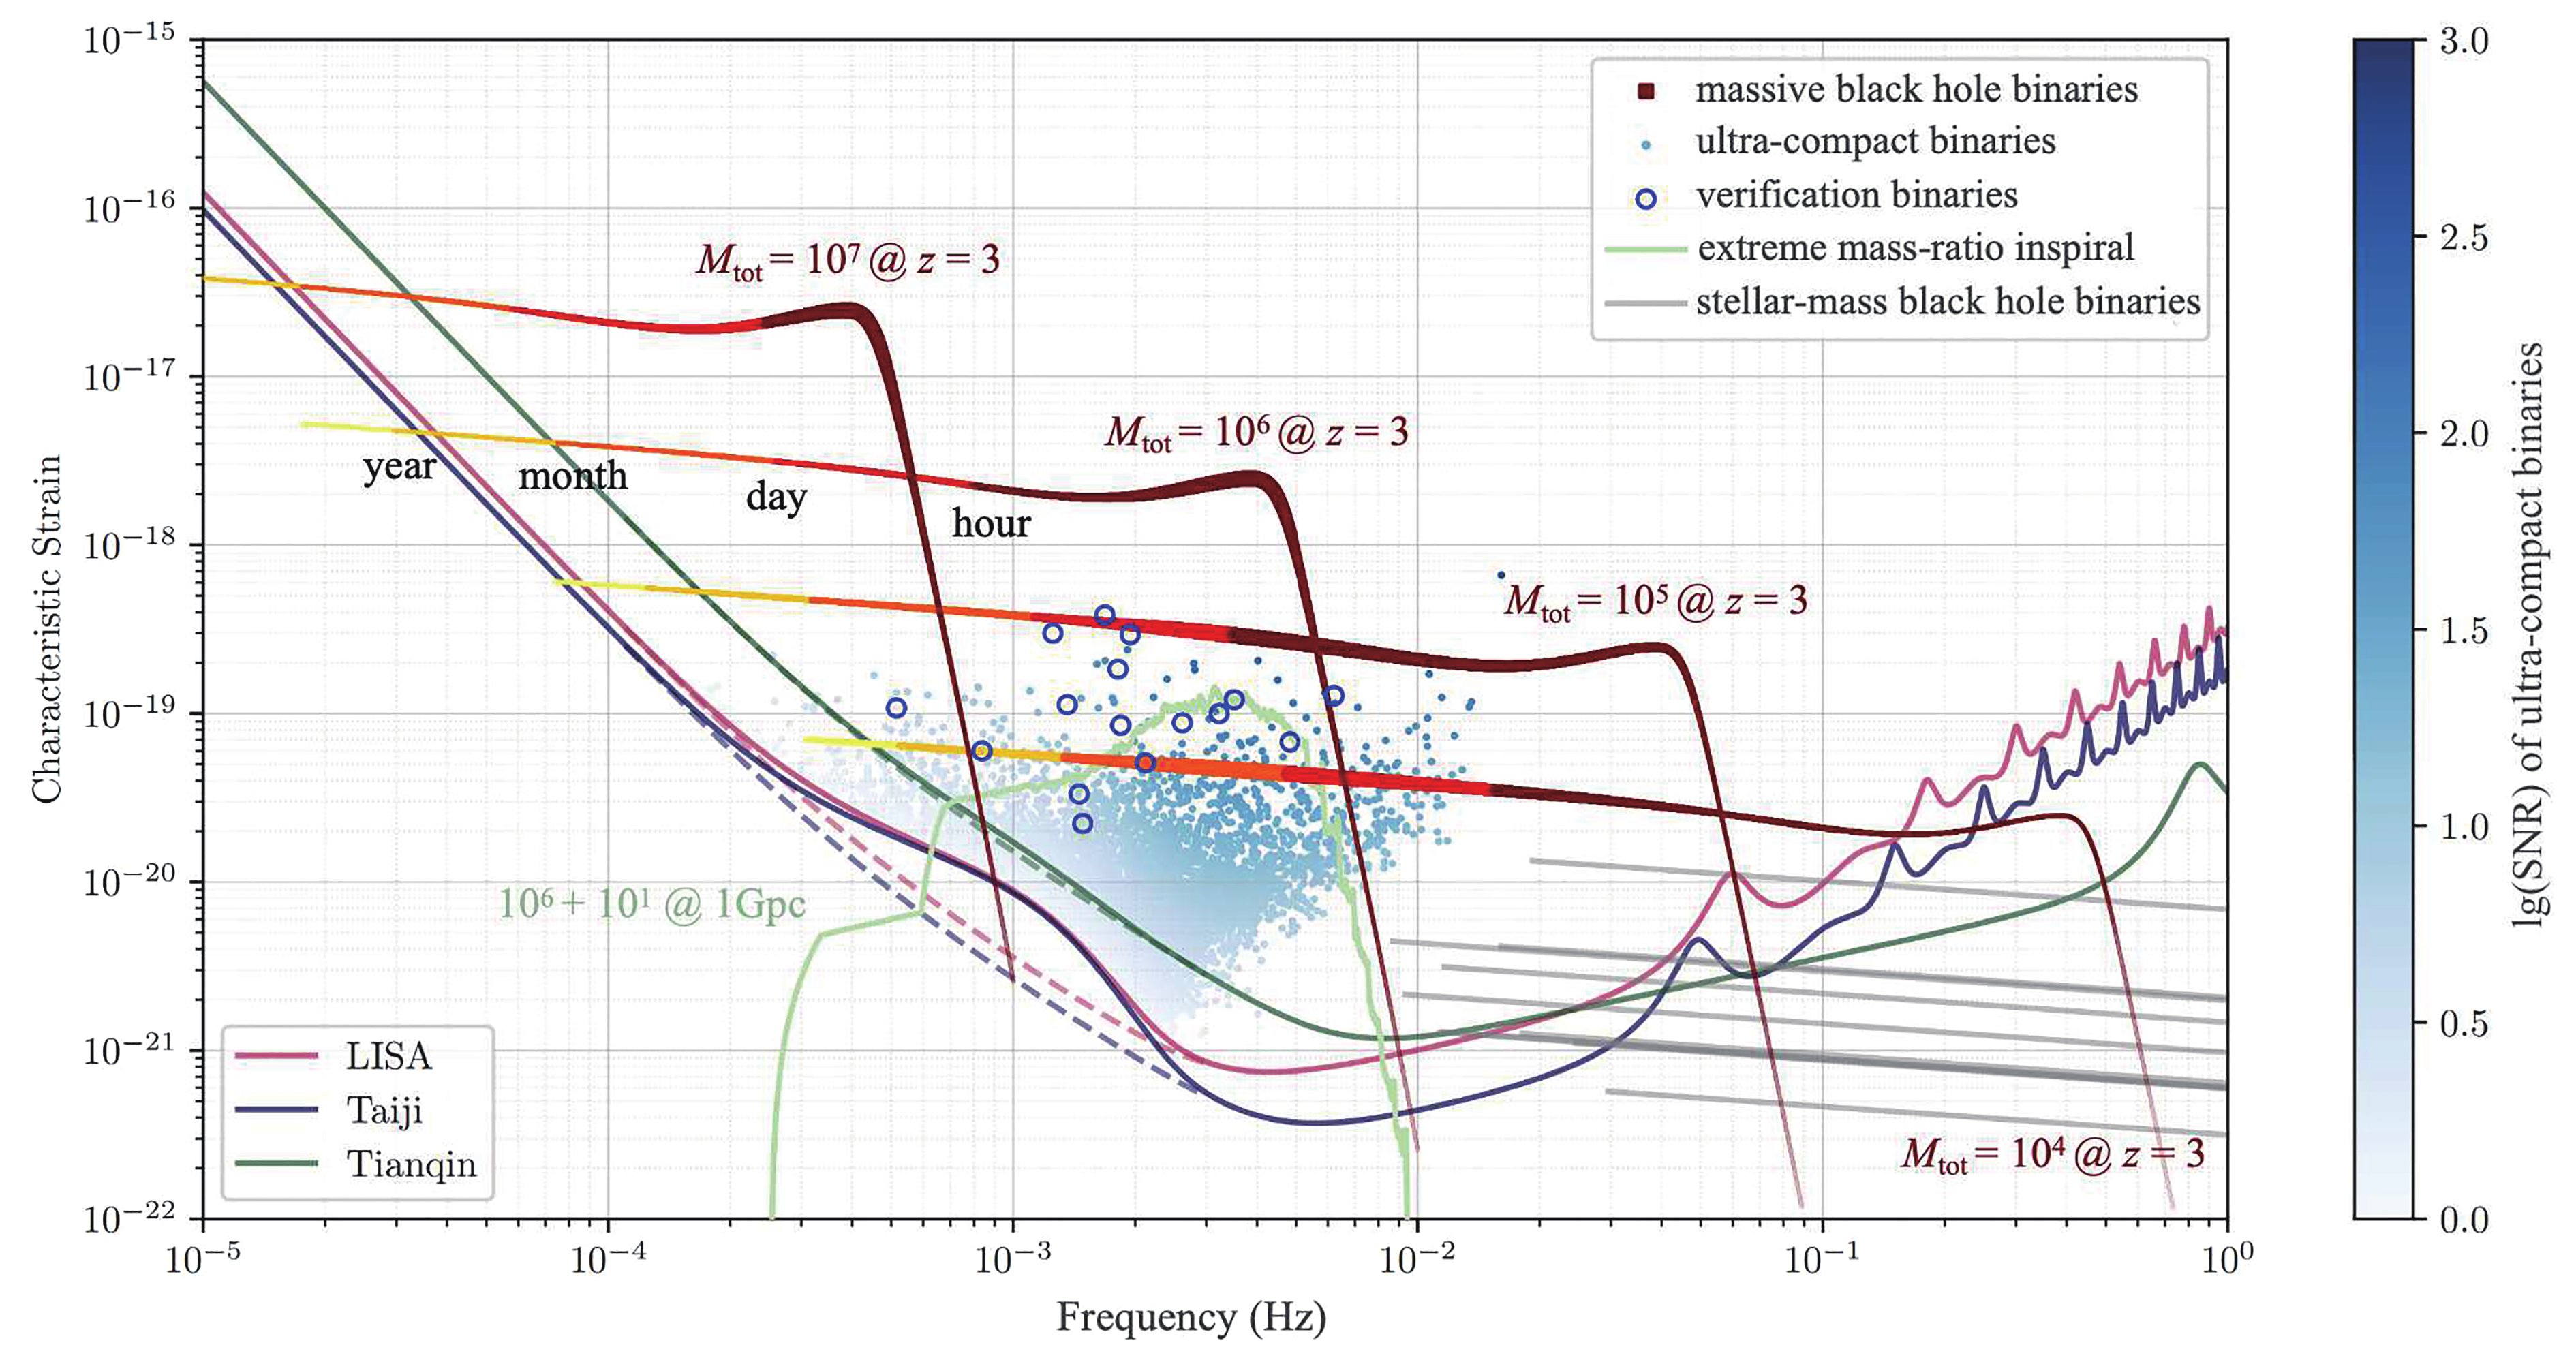
\includegraphics[width=0.98\textwidth]{figures/SSPMA2024_0087_fig1.png}
\caption{空间引力波探测器 LISA、太极和天琴的设计灵敏度曲线及主要目标波源。各探测器灵敏度按等臂长近似下第一代 Michelson-AET 通道的总灵敏度给出，纵轴为特征应变；虚线表示仅计入探测器设备噪声，实线表示加入银河系前景噪声后的结果。图中同时标示大质量双黑洞（MBHB）、超致密双星（UCB）、验证双星（VB）、极端质量比旋入（EMRI）和恒星级质量双黑洞（SBHB）等典型源类，用于说明空间引力波频段内多类源和前景噪声的共同存在。图引自王赫等~\cite{wang2024challenges}的 Figure 1。}
\label{fig:global_fit_signals}
\end{figure}

地面引力波探测器通常每隔数天至数周探测到一个引力波事件，不同事件在时间上不重叠，可以逐一分析。空间引力波探测器则面临截然不同的情形：图~\ref{fig:global_fit_signals} 所示的毫赫兹频段内，LISA、太极和天琴不仅要面对仪器噪声，还要同时面对银河系前景噪声以及多类可分辨天体源。银河系中预计存在约 $10^7$--$10^8$ 个双白矮星系统，其中大约 $10^4$ 个在 LISA/太极的灵敏频段内可分辨，其余形成无法单独区分的“混淆噪声”背景。这一背景本身既是科学目标（可从中提取银河系结构信息），也是分析其他信号的主要干扰。

在混淆噪声背景上，大质量双黑洞并合、EMRI、SBHB 以及验证双星等信号的探测和参数估计需要同时建模背景和感兴趣信号，形成高度耦合的推断问题。尤其是 MBHB 曲线在图中呈现从年、月、日到小时尺度的频率演化轨迹，说明同一源在任务期间会跨越较宽频段，并与其他长期存在的双星前景发生重叠。这与地面探测器中相对“干净”的短时事件环境形成鲜明对比。

信号重叠还体现在时间上：对于持续时间长达数年的 EMRI 信号，其在频域与数千个其他信号叠加，无法通过简单的时域截窗分离。任何针对单个信号的分析都必须同时对其他信号进行建模或减除。

\subsection{混淆噪声的统计特征}

银河系双星混淆噪声在频域具有独特的统计特征。在LISA/太极的低频端（$f \lesssim 3\,\mathrm{mHz}$），可分辨双星的密度很高，混淆噪声可以视为准连续背景，其功率谱密度 $S_\mathrm{conf}(f)$ 可用解析模型近似描述。在高频端（$f \gtrsim 5\,\mathrm{mHz}$），可分辨双星数量减少，混淆噪声逐渐离散为单个可识别的信号。

这种频率依赖特性对数据分析策略有直接影响：在低频段，混淆噪声本质上是一种额外的“有色噪声”，需要与仪器噪声一并建模；在高频段，单个双星信号的参数估计需要同时对相邻频率的其他双星进行建模，形成计算上的“连锁效应”。

全局拟合框架的目标是在统一模型中联合估计主要可分辨信号及噪声背景参数。假设可分辨双星数量为 $N_\mathrm{GB} \approx 10^4$，每个双星有 7-8 个参数，则仅银河系双星部分的参数空间维度已达 $7 \times 10^4$。加上数十个 EMRI（每个17维）和偶发的 MBHB（11维），总维度可以超过 $10^5$，使直接套用传统贝叶斯采样方法变得极为困难~\cite{wang2024challenges}。

\subsection{迭代减除的局限}

当前处理多源叠加问题的常见策略之一是迭代减除（iterative subtraction）：按信号强度从高到低依次估计和减除较强或较易分离的信号，并在残差中继续搜索和建模其他成分。这一策略的可行性依赖两个关键假设：其一，各类信号的信噪比存在足够的层级结构（MBHB 的信噪比通常高于 EMRI，EMRI 又可能高于许多单个银河系双星）；其二，每步减除的精度足够高，不会在残差数据中留下显著的系统误差。

然而，这两个假设在实际中都面临挑战。EMRI 和银河系双星的信噪比范围存在重叠，使得信号层级并不总是清晰；而参数估计的系统误差（尤其是 SBI 方法的近似误差）会在迭代减除中逐步积累，可能使后续步骤的分析严重偏差。

多源分离问题还涉及一个深刻的统计困难：引力波信号的叠加是相干的（即信号直接在时域/频域相加），而非功率叠加（如各向同性随机背景的处理方式）。这意味着个别信号之间存在干涉效应：如果两个频率相近的银河系双星信号发生相消干涉，其联合幅度可能低于单个信号的幅度，导致两者均被漏检。反之，相长干涉可能产生虚假的“强信号”。在约 $10^4$ 个可分辨双星同时存在的频率范围内，这些干涉效应不可忽略，要求多源分离算法显式处理信号间的相干性，而非简单地将各信号视为统计独立。这一相干多源分离问题在信号处理理论中被称为盲源分离（BSS），其计算复杂度随源数目指数增长，进一步凸显了全局拟合问题的难度。

深度学习方法在多源信号分离领域展现出独特优势，尤其是在非线性特征提取和高维映射方面。注意力机制（attention mechanism）使神经网络能够在处理每个信号时动态聚焦于数据中与该信号最相关的时频区域，从而实现对混叠信号的高效分离。Transformer架构通过自注意力层建立长程时频依赖关系，特别适合处理EMRI信号这类具有复杂长时结构的信号。在模拟数据测试中，基于Transformer的多源分离网络在同时存在3--5个银河系双星信号的场景下，成功恢复了各信号参数，估计精度与逐一分析（忽略其他信号）相比误差仅增加约20\%。然而，从3--5个信号扩展到 $10^4$ 个信号的全局拟合场景，仍然是当前深度学习方法面临的开放挑战，需要在网络架构设计和训练策略上的进一步创新。

当前具有代表性的全局拟合路线包括基于RJMCMC（可逆跳转MCMC）与神经网络的混合算法。RJMCMC允许在具有不同参数维度的模型之间进行采样，通过“出生”（birth，向当前模型中添加一个新信号）和“死亡”（death，从当前模型中删除一个信号）步骤，自动适应信号数目。将神经网络训练为高效的候选生成器或提议分布，可在RJMCMC的若干步骤中快速评估候选信号添加或删除的可能性，从而有望将特定模拟设置下的全局拟合计算时间压缩到更可操作的尺度。ESA LISA数据挑战（LDC2a）的相关结果表明，这类混合方法在处理含数十个以上银河系双星的模拟数据时已展现出可行性，为未来太极/LISA实际数据分析提供了重要方法参照。

\section{非平稳噪声下的信号检测困难}

匹配滤波的最优性依赖于高斯平稳噪声假设。真实探测器噪声的非平稳特性从两个层面破坏这一假设。

\textbf{短时暂态噪声（glitch）}：LIGO-Virgo 每小时约产生数个明显的 glitch，其幅度可比背景噪声高出一至两个量级，持续时间从毫秒到秒不等。glitch 与引力波信号的区分主要依赖于：两台探测器的耦合检验（引力波在两台探测器中应以光速传播的时延出现）、$\chi^2$ 时频检验（引力波的时频演化应与模板一致）、以及机器学习分类器（Gravity Spy 等）。尽管这些方法已大幅降低误报率，glitch 的存在仍是引力波搜索中最主要的系统误差来源。

\textbf{长时噪声漂移}：探测器的灵敏度曲线（即功率谱密度 $S_n(f)$）在数小时到数天的时间尺度上缓慢变化，由于环境条件（温度、地震、激光功率）的波动。匹配滤波通常假设 $S_n(f)$ 在分析时段内不变，噪声漂移会导致信噪比估计偏差。在线分析中，$S_n(f)$ 需要从近期数据实时估计并滚动更新，引入额外的不确定性。

空间引力波探测器的非平稳噪声更为复杂：数据间隙（卫星维护期间的数据缺失）、仪器暂态（激光锁定失调等）、以及时变噪声自相关（轨道运动导致的热噪声周期性变化）。Xu 等人~\cite{xu2024nonstationarty} 的工作表明，即便是先进的深度学习方法，在面对这三类非稳态噪声时也需要专门的鲁棒性设计。

\subsection{Glitch 分类与机器学习}

glitch 的自动分类是引力波数据质量控制的重要组成部分。Gravity Spy 是目前最广泛使用的 glitch 分类系统，基于卷积神经网络对 Q 变换时频图进行多类别分类，能够识别数十种已知 glitch 类型（blip、koi fish、scattered light、violin mode 等）。

glitch 分类的挑战在于：已知类型的 glitch 可以通过监督学习有效识别，但真实探测器中不断出现新的未知 glitch 类型，需要持续的人工标注和模型更新。此外，部分 glitch 类型（如 blip）在时频形态上与短持续时间的引力波信号（如高质量双黑洞并合）高度相似，是误报率的主要来源之一。

MF-CNN 方法~\cite{wang2020deeplearning} 在 O1 数据上的 glitch 分析表明，将匹配滤波物理先验嵌入网络结构，能够显著提升对 blip、koi fish 等常见 glitch 类型的筛查率，这是纯 CNN 方法所不具备的优势。这一结果进一步支持了物理-数据融合方法在噪声鲁棒性方面的优越性。

辅助通道（auxiliary channel）监测是引力波探测器中噪声溯源和glitch特征化的核心工具。LIGO探测器运行期间同时记录约2万个辅助通道，包括地震仪、磁强计、激光功率监测器、腔体控制误差信号等，这些通道反映了探测器周边环境和内部子系统的状态。当主通道（引力波应变信号 $h(t)$）出现glitch时，分析辅助通道数据可以识别噪声来源：若某个辅助通道在glitch发生约1毫秒前出现异常（考虑信号传播时延），则该通道对应的物理过程是glitch的可能来源。iDQ（idq）系统是自动化辅助通道分析的代表工具，通过机器学习在辅助通道数据中实时学习glitch的预测指标，将主通道glitch的预测置信度实时推送给在线搜索流水线，使流水线能够动态调整信噪比阈值，在glitch活跃时段降低灵敏度以减少误报。在O3观测中，iDQ系统成功识别了约60\%的已知glitch类型，将相应时段的误报率降低约50\%，是glitch减除的重要辅助工具。

噪声的空间相关性也是引力波分析中值得关注的非平稳特征。Schumann共振（Schumann resonances）是地球电磁场的准全球性共振模式，频率约7.8 Hz及其谐波（14.3、20.8 Hz……），由闪电激发。Schumann共振在两台相距数千公里的LIGO探测器之间可以引起磁噪声的相关涨落，从而产生虚假的引力波信号相干性。实际上，在引力波候选事件的后处理分析中，必须对磁场辅助通道进行相关性检验以排除Schumann共振来源。O3期间，LIGO合作组对所有候选事件系统性地进行了磁场相关性分析，未发现任何事件与Schumann共振显著相关，但这一检验本身的建立就反映了非平稳噪声分析的复杂性。

\subsection{噪声非平稳性的量化描述}

噪声非平稳性的定量描述对于理解其对数据分析的影响至关重要。常用的量化指标包括：

\textbf{功率谱密度的时变性}：将数据分段（通常每段 $\sim$ 4 秒至 32 秒），对每段估计局部 PSD，比较不同时段的 PSD 差异。若 PSD 在相邻时段变化超过某个阈值（如 10\%），则认为该段数据存在显著的非平稳性，需要特殊处理。

\textbf{非高斯性指标}：计算数据的峰度（kurtosis）$\kappa = \langle x^4 \rangle / \langle x^2 \rangle^2$，高斯分布的峰度为3，$\kappa > 3$ 表明存在重尾分布（即 glitch 引起的非高斯成分）。LIGO 数据的峰度通常在 3.1-3.5 之间，而 glitch 活跃时段可超过 10。

\textbf{Anderson-Darling 检验}：对白化数据进行正态性统计检验，在滑动窗口内追踪检验统计量的变化。这一方法在 PyCBC 等实际搜索流水线中用于实时标记数据质量。

理解这些定量指标，不仅有助于评估经典方法的适用性，也为机器学习方法的训练数据设计提供了重要参考：高质量的训练数据应当包含与真实探测器统计特性相符的噪声样本，其峰度、功率谱密度的时变特征都需要与真实数据吻合。

非平稳噪声对统计推断的影响不仅体现在信号检测的误报率上，还深刻影响参数估计的精度和准确性。在参数估计框架中，引力波似然函数 $\ln p(d|\theta) = -\frac{1}{2}\langle d-h(\theta), d-h(\theta)\rangle$ 中的内积使用噪声功率谱密度 $S_n(f)$ 作为权重。若 $S_n(f)$ 的估计存在偏差（由于噪声非平稳性），则似然函数值将系统性地偏离真实值，导致后验分布的偏移。定量地，若噪声PSD在信号观测期间相比估计期间增大了 $\epsilon$（相对变化），则参数估计的系统偏差约为 $\sigma_\theta \times \epsilon/\mathrm{SNR}$，其中 $\sigma_\theta$ 是参数的统计不确定度，$\mathrm{SNR}$ 是信号信噪比。对于典型的 $\epsilon \sim 5\%$（探测器在数小时内的PSD漂移幅度）和 $\mathrm{SNR} \sim 15$，系统偏差约为统计不确定度的0.3\%，通常可以忽略。但对于低SNR事件（$\mathrm{SNR} \sim 5$--$8$），系统偏差可达统计不确定度的数十\%，需要显式的PSD不确定度建模。

空间引力波探测器的噪声非平稳性具有独特的物理来源，区别于地面探测器。太极/LISA的主要噪声来源包括：残余加速度噪声（来自卫星上残余气体的随机碰撞和太阳辐射压力的涨落，在低频段按 $f^{-2}$ 增长）、光学路程噪声（激光测距的散粒噪声，在高频段接近白噪声）、以及TDI残差（激光频率噪声经TDI消除后的残留，与臂长估计误差有关）。这些噪声源在一年的任务运行周期内都会随时间缓慢变化，特别是残余加速度噪声受卫星热控系统状态的影响，可能在任务中期出现系统性的噪声功率变化（估计约$\pm 20\%$）。深度学习去噪方法（第7章）通过在训练集中引入时变噪声模拟样本，使模型对这类变化保持鲁棒性，而相关系统研究表明，即便在三类非稳态噪声同时存在的混合情形下，鲁棒去噪模型的重叠度仍可维持在0.92以上，远优于非鲁棒模型的0.51。这一结果表明，噪声鲁棒性的设计不应视为数据预处理的附属问题，而是方法论设计的核心要求。

在数据质量控制的实际操作层面，引力波合作组维护着详细的数据质量标志（Data Quality Flags，DQF）系统，对不同类型的噪声非平稳事件进行标记。这些标志按照严重程度分为三级：Category 1（CAT1）标志对应仪器故障期间的数据，必须在任何分析中排除；Category 2（CAT2）标志对应已知噪声来源（如散射光噪声、控制噪声）造成的短时扰动，通常在离线分析中排除；Category 3（CAT3）标志对应统计测试发现的轻微非平稳性，由分析者根据具体场景决定是否排除。在O3观测轮次中，约有5\%--10\%的数据因数据质量标志而被从最终分析中排除，这一比例的存在本身即反映了真实探测器噪声环境的复杂性。

噪声非平稳性对机器学习方法的挑战，比其对经典方法的挑战更为根本。经典匹配滤波通过实时更新噪声PSD估计来适应噪声变化，这一在线更新机制是流水线设计的内置组件；但机器学习模型通常在训练完成后以固定参数运行，无法在推断时实时更新噪声模型。这意味着，若真实噪声在运行期间发生了超出训练分布的变化，机器学习模型的性能将悄无声息地退化，而无法像经典方法那样通过显式的噪声跟踪机制发出警告。应对这一挑战的策略包括：在训练集中引入噪声状态变化的系统性模拟（Xu等的鲁棒去噪框架，第7章）；设计在线性能监控系统，定期用已知信号注入测试检验模型性能；以及建立模型更新触发机制，当性能监控检测到显著退化时自动启动模型微调。这些工程机制的设计，是机器学习方法走向引力波天文台生产环境的重要保障，也是第10章讨论的系统工程挑战的重要组成部分。

汇总前三节的分析，可以得到引力波数据分析可扩展性瓶颈的全貌。这里给出计算复杂性的系统整理。

\section{计算复杂性与可扩展性边界}

在信号搜索层面，匹配滤波的计算量为 $O(N_\mathrm{template} \times N_\mathrm{data})$，其中模板数 $N_\mathrm{template}$ 随自旋参数的加入从 $10^4$ 增至 $10^6$，使低延迟（在线）完整自旋搜索在计算上困难。

在参数估计层面，MCMC/嵌套采样的计算量约为 $O(N_\mathrm{eval} \times T_\mathrm{waveform})$，其中 $N_\mathrm{eval}$ 为似然评估次数（通常 $10^6$--$10^7$），$T_\mathrm{waveform}$ 为单次波形生成时间（地面双黑洞 $\sim 1$ ms，空间 EMRI $\sim 1$--100 s）。若采用计算较慢的精细EMRI波形模型，参数估计总时间可达 $10^6 \times 100\,\mathrm{s} \approx 3$ 年量级，明显超出常规科学分析的可接受范围。

在全局拟合层面，空间引力波探测器的联合参数估计维度 $\sim 10^7$，对任何已知的采样方法都构成根本性挑战。Liang 和 Wang~\cite{liang2026sbireview} 的综述明确指出，SBI 方法是解决这一计算瓶颈的当前最有前景的路径。

引力波波形生成（waveform generation）是似然函数评估的主要计算瓶颈，其计算代价因波形近似方法的不同而有数个量级的差异。最快的波形近似是频域后牛顿（PN）模型（如TaylorF2），通过解析公式直接计算频域波形，单次生成时间约0.1毫秒，但精度有限（在高质量比或强场区域偏差较大）。更精确的有效单体（EOB）模型（如SEOBNRv4）通过数值求解常微分方程组生成波形，单次计算时间约1--10毫秒，是当前参数估计的主力波形模型。精度最高但计算最慢的是数值相对论（NR）波形，通过求解完整的爱因斯坦场方程获得，单次计算需要数小时至数天，只用于校准其他波形模型的参数，而非直接用于MCMC采样。

机器学习替代波形（ML surrogate waveform）是近年来显著加速参数估计的重要技术路线。通过在预先计算的波形数据库上训练高斯过程回归或神经网络模型，可以构建原始波形的高精度替代（surrogate），其评估速度比原始EOB模型快约100--1000倍（约0.01--0.1毫秒），同时精度损失通常在1\%以内（以平均相位误差衡量）。NRSurrogate系列模型是当前最精确的替代波形，通过对约1400条数值相对论波形的稀疏表示学习，实现了对非旋进双黑洞波形的高精度快速评估，已被集成到LALSuite和Bilby框架中。然而，这类替代波形通常只覆盖有限的参数范围（如质量比 $q \leq 6$、总质量约20--200太阳质量），对于极端参数区域仍需回退到EOB或PN模型，这是替代波形方法在通用参数估计中的主要局限。

除了单次波形生成耗时，模板库规模本身也会改变搜索的统计阈值。模板越多，在固定总误报率要求下需要控制的试验因子越大；因此即使每条模板的计算可以通过 FFT、GPU 或降阶基加速，信号达到可确认探测所需的阈值 SNR 仍会随有效模板数上升。Moore、Gerosa 与 Klein 对 LISA 中恒星质量双黑洞的多波段探测问题给出了一个清晰例子：若把长寿命、啁啾缓慢的 LISA 信号作为大模板库搜索问题处理，恒星质量双黑洞的有效模板库规模远大于地面探测器中的常规双黑洞搜索，理想化搜索下的阈值 SNR 可升至 $\rho_\mathrm{thr}\sim14$--15；EMRI 搜索则需要更大的有效模板库，阈值可进一步提高~\cite{Moore2019StellarMassLISA}。这说明可扩展性瓶颈并不只表现为“算得慢”，还会通过背景试验因子和检测阈值影响可探测源数。

\begin{figure}[htbp]
\centering
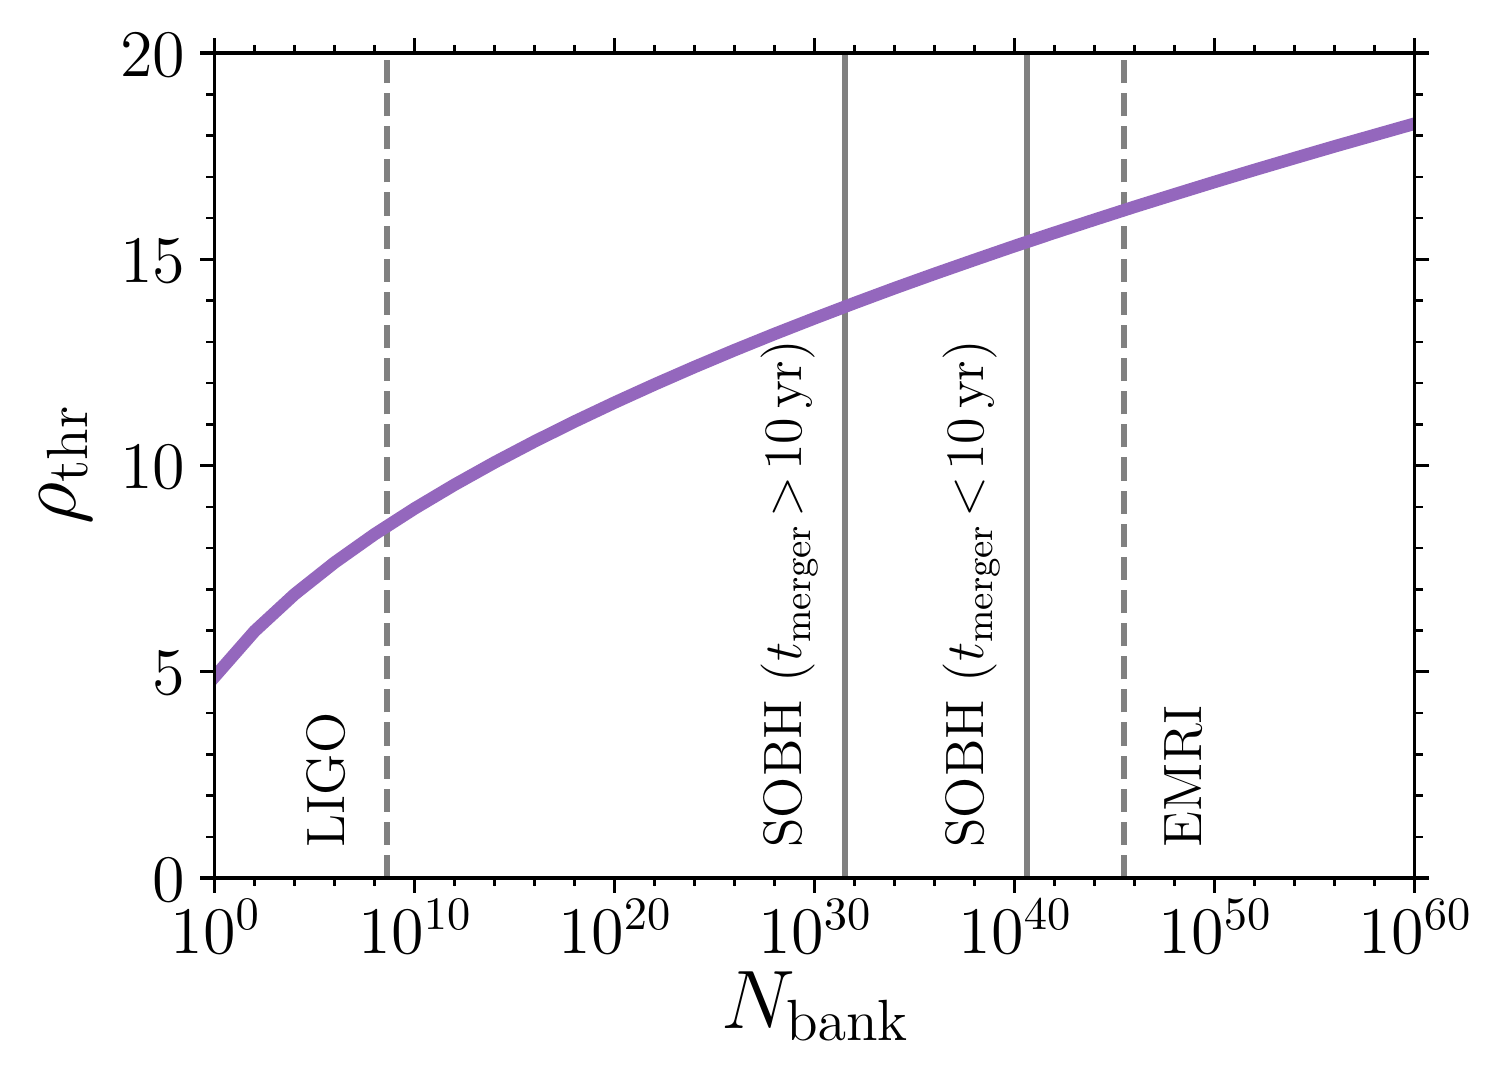
\includegraphics[width=0.82\textwidth]{figures/MNRASL2019_slz104_fig1.png}
\caption{模板库规模对引力波搜索阈值 SNR 的影响。横轴为有效模板数 $N_\mathrm{bank}$，纵轴为在固定误报控制下所需的阈值 SNR；图中竖线比较了 LIGO/Virgo 双黑洞搜索、LISA 中恒星质量双黑洞（SOBH）快慢啁啾情形以及 EMRI 搜索的典型模板库规模。该图表明，空间探测器中的长寿命信号会显著放大模板库规模和试验因子，使可探测阈值从地面探测器常见的 $\rho\sim8$ 提高到 $\rho_\mathrm{thr}\sim14$--15，甚至更高。图引自 Moore、Gerosa 与 Klein~\cite{Moore2019StellarMassLISA} 的 Figure 1。}
\label{fig:dim_compute_cost}
\end{figure}

\begin{table}[htbp]
\centering
\caption{引力波数据分析计算代价随任务复杂度的变化}
\label{tab:compute_complexity}
\small
\begin{tabular}{lcccc}
\hline
\textbf{任务} & \textbf{参数维度} & \textbf{似然评估次数} & \textbf{单次波形时间} & \textbf{总时间} \\
\hline
地面 BBH 搜索 & $\leq 2$ & — & $\sim 1$ ms & 近实时 \\
地面 BBH 参数估计 & 15 & $\sim 10^7$ & $\sim 1$ ms & $\sim 22$ 小时 \\
太极 MBHB 参数估计 & 11 & $\sim 10^7$ & $\sim 10$ ms & $\sim 30$ 小时 \\
太极 EMRI 参数估计 & 17 & $\sim 10^7$ & $\sim 1$--$100$ s & 月级至年级 \\
空间引力波全局拟合 & $10^5$--$10^7$ & — & — & \textbf{当前难以直接采样} \\
\hline
SBI 推断（BBH） & 15 & $\sim 1$（推断） & — & $\sim 1$ 秒 \\
SBI 推断（EMRI）& 17 & $\sim 1$（推断） & — & $\sim$ 秒至分钟 \\
\hline
\end{tabular}
\begin{minipage}{\linewidth}
\vspace{1mm}
\small 注：SBI 方法需要离线训练阶段（约数小时至数天），但推断阶段对新观测数据只需秒级响应。
\end{minipage}
\end{table}

从计算复杂性理论的角度，引力波数据分析中的核心计算瓶颈属于不同的复杂度类别，值得系统区分。模板匹配（信号搜索）属于可以利用FFT加速的线性计算问题，其复杂度 $O(N_T \times N_d \times \log N_d)$（$N_T$ 为模板数，$N_d$ 为数据点数）虽然随模板数线性增长，但GPU并行化可以将有效计算时间压缩到现实可接受范围（在高速GPU集群上对 $10^6$ 条模板的在线搜索约需数秒）。这类问题属于“计算困难但工程上可解决”的类别，在算法设计上仍有较大的优化空间。

与此形成鲜明对比，贝叶斯后验采样（参数估计）的并行化效率受到采样相关性的限制：MCMC单链的第 $k$ 步状态依赖第 $k-1$ 步，不能简单通过增加似然评估节点线性缩短墙钟时间。虽然多链并行、并行回火、动态嵌套采样和并行似然计算都能显著改善实际效率，但总的有效样本数、链混合时间和收敛诊断仍然构成关键瓶颈。对于17维EMRI参数估计，若采用精细波形并要求充分探索强简并、多模态后验，墙钟时间可能达到月级至年级。这类问题的困难并不只是硬件不足，而在于推断流程本身带有显著的序列相关性；SBI方法将大量计算转移到可并行的训练阶段，为绕开这一瓶颈提供了新的方法论路径。

全局拟合的高维参数估计则属于更高层次的挑战：不仅存在采样困难，而且似然函数本身的计算也极为昂贵（需要同时评估大量信号的TDI响应）。若以完整MCMC直接处理全局拟合作为粗略估计，在 $10^5$--$10^7$ 维参数空间中实现充分混合可能需要远超常规任务预算的采样步数；每步代价还随信号数目和响应模型复杂度增长。这不是单纯增加硬件即可解决的工程困难，而是需要重新组织推断流程的方法论挑战。SBI方法将这一“直接采样难以承担”的问题转化为“训练可并行、推断需校准”的问题，是方法论层面的范式转变，而非单纯的工程优化。理解这一区别对于正确评估SBI方法的意义至关重要：SBI不是对现有方法的小幅性能优化，而是为此前难以直接处理的问题开辟一条可检验的近似路径。

计算复杂性分析还揭示了引力波数据分析中一个重要的不对称性：训练代价与推断代价的分离。神经网络推断的“在线”代价（对新观测数据的前向传播）通常较低，且与参数空间维度弱相关；但“离线”训练代价（在模拟数据上优化网络参数）可达数天至数周，且随问题复杂度增加。对于太极/LISA全局拟合，即便是SBI的训练阶段也面临巨大挑战：训练数据的生成需要大量模拟，模拟器本身的运行时间可从秒级到小时级不等，生成足够大的训练集需要消耗大量分布式计算资源。然而，这一训练代价可以被摊销到大量后续推断任务中，且训练阶段高度可并行化（不同训练样本的模拟可以在不同计算节点上独立运行）。这种“离线大代价换在线低代价”的模式，从根本上改变了引力波数据分析的计算经济学。

高维参数空间的可扩展性危机，还驱动了波形生成技术本身的重要改进。传统的后牛顿波形模型（IMRPhenomX、SEOBNRv4等）通过解析公式直接计算波形，速度约为毫秒量级，但精度受限于后牛顿展开的有限阶次。为了在更高精度下保持计算效率，还原阶模型（reduced order models，ROM）技术通过对大量预计算的精确波形进行奇异值分解（SVD），建立低维参数化表示，将波形生成速度提升约100倍同时保持接近数值相对论的精度。机器学习代理波形（surrogate models）则进一步利用深度学习对高维波形流形进行非线性建模，将波形生成速度提升约1000倍，同时在整个参数空间内保持约 $10^{-3}$ 的相位误差。对于EMRI波形，快速EMRI波形（FastEMRIWaveforms，FEW）框架通过预计算大量基底波形并以稀疏表示重建，将单次EMRI波形生成从数小时压缩至约1秒，是使SBI-EMRI参数估计在计算上可行的关键使能技术。这些波形生成技术的改进，与SBI推断方法的改进相辅相成：更快的波形生成使SBI训练集的构建更高效，而SBI方法的高效推断又降低了对波形生成速度的要求，两者共同推动引力波参数估计走向实用化。

本章的分析揭示了一个核心结论：引力波数据分析面临的挑战不仅是精度问题，更是可扩展性问题。经典方法在精度和透明性上具有明确优势，但其计算复杂度在面向空间引力波探测器时会迅速超出现实预算。这一认识为后续各章的AI方法提供了清晰的问题定位。神经网络的训练虽然代价高昂，但推断速度很快；一旦训练完成，对新数据的分析时间通常随参数空间维度增长较弱，从而改变了可扩展性的约束条件。

值得特别强调的是，“可扩展性危机”并不意味着“精度足够”。引力波数据分析的双重挑战——同时满足高精度要求和高可扩展性要求——是任何方法都难以在不妥协的前提下同时实现的。贝叶斯推断在统计严格性上具有明确优势，但在可扩展性上受到限制；人工智能方法在推断速度上优势显著，但在精度校准和域外泛化上存在近似误差。“精确协同”范式（第9章的核心主题）的价值正在于此：通过将两者有机结合，在精度和可扩展性之间寻找可验证的折中方案。这一折中点随技术的进步而演化：更精确的SBI方法（更好的归一化流架构）、更高效的精确贝叶斯方法（更快的波形生成）、以及更强大的计算资源，将共同推动方法体系向既精确又高效的理想方向移动。

未来方法发展的路径图可以从三个维度来描述。第一维是时间维：近期重点建立高保真仿真和标准化验证框架，中期逐步发展面向空间任务的AI分析管道，长期目标是在太极/LISA等任务中形成可校准、可复现的智能化全局拟合系统。第二维是方法维：从单一方法向方法体系演化，从近似方法向精确协同方法演化，从人工设计向自动发现方法演化。第三维是验证维：从经验验证向统计保证演化，从局部验证向全局一致性验证演化，从单任务验证向跨任务通用性验证演化。这三个维度的协同演化，有望在未来十年内推动引力波AI数据分析体系走向成熟。

这一认识为后续各章的 AI 方法提供了清晰的问题定位。第5章的机器学习信号识别、第6章的模拟推断、第7章的去噪、第8章的自动算法发现，均是在这一问题框架下提出的具体解决方案：它们通过降低在线推断成本、改善噪声鲁棒性或扩大算法搜索空间，缓解经典方法在规模化任务中的压力，但其科学使用仍需要统计校准、物理一致性检验和经典方法交叉验证。

值得注意的是，AI 方法并非旨在替代经典方法，而是作为互补工具：快速搜索（AI）为精确参数估计（经典方法）提供初始化，SBI 近似（AI）为全局拟合（经典方法）提供先验约束，自动算法发现（AI）为信号处理管道设计（人工专家）提供候选方案。这种互补关系，正是第9章“物理驱动与数据驱动融合”的核心主题。

\section{数值相对论波形与代理模型}

\subsection{数值相对论波形的必要性}

引力波波形的精确建模是引力波数据分析的基础。在旋近（inspiral）阶段，后牛顿（post-Newtonian，PN）展开提供了系统性的解析近似：将广义相对论方程按照 $v/c$ 的幂次展开，目前已发展至3.5PN阶次，能够精确描述双星系统在轨道分离较大时的引力波辐射~\cite{Blanchet2014PN}。然而，后牛顿展开本质上是弱场慢速近似，其有效性随轨道收缩而迅速下降。当双黑洞系统进入并合（merger）阶段——轨道分离约为几倍史瓦西半径、轨道速度达到 $v/c \sim 0.5$--$0.7$ 时——后牛顿展开的截断误差急剧增大，无法给出可靠的波形预测。

数值相对论（numerical relativity，NR）是在并合阶段获得高精度引力波波形的关键方法。NR通过直接数值求解爱因斯坦场方程的完整非线性形式，无需弱场或慢速近似，从而能够精确捕捉并合阶段的强引力场动力学。2005年，Pretorius首次成功完成了双黑洞并合的全数值相对论模拟~\cite{Pretorius2005NR}，这一突破性工作开启了NR波形系统性研究的新纪元。

NR模拟的计算代价极为高昂。一次典型的双黑洞并合模拟需要在三维自适应网格上求解约 $10^6$--$10^8$ 个网格点的爱因斯坦方程，时间步长受Courant条件约束（约为最小网格间距除以光速），总时间步数约为 $10^4$--$10^6$ 步。单次模拟通常需要数千CPU核时（core-hours），对于高质量比（$q = m_1/m_2 \gg 1$）或高自旋系统，计算代价还会进一步增加一至两个量级。这一计算代价决定了NR波形无法直接用于需要大量波形评估的贝叶斯参数估计或SBI训练，而必须通过代理模型（surrogate models）来实现高效访问。

目前，国际上已建立了多个系统性的NR波形目录。\textbf{SXS目录}（Simulating eXtreme Spacetimes）由加州理工学院、康奈尔大学等机构联合维护，截至2024年已包含超过3000个双黑洞并合模拟，覆盖质量比 $q \leq 10$、自旋幅度 $|\chi| \leq 0.998$ 的参数空间~\cite{Boyle2019SXS}。\textbf{RIT目录}（Rochester Institute of Technology）专注于高自旋和高质量比系统，提供了约1500个模拟，对非对称质量比系统的高阶模式有系统性覆盖~\cite{Healy2022RIT}。\textbf{GeorgiaTech目录}则在高质量比（$q$ 达到15--18）和偏心轨道方向有独特贡献~\cite{Jani2016GeorgiaTech}。这三个目录共同构成了当前NR代理模型训练的主要数据来源，其波形数据通过统一的SXS格式（NRAR格式）公开发布，极大地促进了波形建模社区的协作。

\subsection{NR波形的主要物理特征}

NR波形揭示了并合阶段若干在后牛顿近似中无法捕捉的重要物理特征，这些特征对引力波数据分析具有直接影响。

\textbf{并合阶段的非线性效应}。在最终并合前约5--10个轨道周期内，引力场的非线性效应变得不可忽略。引力波的辐射功率在并合时刻达到峰值，约为 $10^{56}$ erg/s（约为太阳光度的 $10^{22}$ 倍），这一峰值功率本身就是强非线性效应的体现。NR模拟还揭示了“引力波记忆”（gravitational wave memory）效应——并合后时空的永久形变——以及并合过程中的非线性模式耦合，这些效应在后牛顿框架中均无法系统描述。

\textbf{铃宕阶段的准简正模}。并合后形成的扰动克尔黑洞通过辐射引力波而弛豫至稳态，这一过程称为铃宕（ringdown）。铃宕阶段的引力波可以用准简正模（quasi-normal modes，QNM）展开描述：
\begin{equation}
  h(t) = \sum_{\ell m n} A_{\ell m n} \, e^{-t/\tau_{\ell m n}} \cos\!\left(2\pi f_{\ell m n} t + \phi_{\ell m n}\right),
\end{equation}
其中 $(\ell, m)$ 为球谐模式指标，$n$ 为泛音（overtone）指标，$f_{\ell m n}$ 和 $\tau_{\ell m n}$ 分别为QNM频率和衰减时间，由末态黑洞的质量 $M_f$ 和自旋 $\chi_f$ 唯一确定（黑洞无毛定理）。主导模式为 $(\ell, m, n) = (2, 2, 0)$，其频率约为 $f_{220} \approx 32\,\mathrm{kHz} \times (M_\odot/M_f)$，衰减时间约为 $\tau_{220} \approx 0.55\,\mathrm{ms} \times (M_f/M_\odot)$。通过测量QNM频率和衰减时间，可以检验广义相对论的黑洞无毛定理（黑洞谱学，black hole spectroscopy），这是引力波天文学的重要科学目标之一。

\textbf{高阶模式的重要性}。引力波辐射可以分解为自旋权重为 $-2$ 的球谐函数 ${}_{-2}Y_{\ell m}(\iota, \varphi)$ 的叠加：
\begin{equation}
  h_+ - \mathrm{i} h_\times = \sum_{\ell \geq 2} \sum_{|m| \leq \ell} h_{\ell m}(t) \, {}_{-2}Y_{\ell m}(\iota, \varphi),
\end{equation}
其中 $\iota$ 为轨道倾角，$\varphi$ 为方位角。对于等质量系统（$q = 1$），主导模式 $(\ell, m) = (2, \pm 2)$ 贡献了约99\%的辐射功率，高阶模式（higher-order modes，HOM）可以忽略。然而，对于非对称质量比系统（$q \gg 1$），高阶模式的相对贡献显著增大：$q = 4$ 时 $(3,3)$ 模式贡献约10\%，$q = 8$ 时贡献约20\%，$q = 18$ 时贡献可达30\%以上~\cite{Cotesta2018HOM}。忽略高阶模式将导致系统性的参数偏差：质量比、距离和倾角的测量误差可达数十个百分点。随着LIGO-Virgo-KAGRA探测到越来越多的非对称质量比事件（如GW190412、GW190814），高阶模式的精确建模已成为波形模型的必要组成部分。

\subsection{代理模型：从NR到快速波形生成}

NR波形的高精度与高计算代价之间的矛盾，催生了代理模型（surrogate models）这一重要技术路线。代理模型的核心思想是：利用有限数量的NR模拟（训练集），通过插值或机器学习方法，构建能够在任意参数点快速生成高精度波形的近似模型。

\textbf{高斯过程回归代理}。早期代理模型采用高斯过程回归（Gaussian process regression，GPR）对NR波形的幅度和相位进行参数空间插值。GPR的优势在于提供不确定度估计（预测方差），允许量化代理模型在训练集稀疏区域的外推误差。然而，GPR的计算复杂度随训练集大小 $N$ 以 $O(N^3)$ 增长，限制了其在高维参数空间中的可扩展性。

\textbf{NRSurrogate系列}。Blackman等人提出的NRSurrogate方法将降阶建模（reduced order modeling，ROM）与GPR相结合，实现了对NR波形的高效代理~\cite{Blackman2017NRSur}。其核心步骤包括：（1）对训练集NR波形进行奇异值分解（SVD），提取主要正交基向量（通常约100--200个基向量即可捕捉99.99\%的波形方差）；（2）对每个基向量的系数在参数空间中进行GPR插值；（3）通过线性组合重建任意参数点的波形。

\textbf{NRSur7dq4}是常用的NR代理模型之一，覆盖质量比 $q \leq 4$、任意自旋方向（7维参数空间：质量比 $q$，两个自旋矢量各3个分量，共7个参数）~\cite{Varma2019NRSur7dq4}。该模型基于1528个SXS模拟训练，波形生成时间约为0.1--1毫秒（相对直接NR模拟快多个量级），在训练集覆盖的参数空间内，与NR波形的失配（mismatch）约为 $10^{-3}$--$10^{-4}$，通常优于许多解析近似模型在强场进动参数区间的表现。对于高质量比系统，\textbf{NRHybSur3dq8}将质量比范围扩展至 $q \leq 8$，但仅支持对齐自旋（3维参数空间）~\cite{Varma2019NRHybSur3dq8}。

\textbf{神经网络代理}。近年来，深度学习方法被引入波形代理建模，进一步提升了高维参数空间中的插值精度和生成速度。循环神经网络（RNN）和变换器（Transformer）架构被用于直接生成时域波形序列，避免了GPR方法在高维空间中的可扩展性问题。神经网络代理的训练代价较高（通常需要数天GPU时间），但推断速度极快（微秒至毫秒量级），且随参数空间维度的增加，性能退化远慢于GPR方法。

\textbf{代理模型与SBI的协同}。代理模型对SBI方法的实用化具有重要意义。SBI训练需要大量模拟样本（通常 $10^5$--$10^7$ 个），每个样本需要生成一条完整的引力波波形。若使用直接NR模拟（每次数千CPU核时），生成 $10^6$ 个训练样本需要约 $10^9$ CPU核时，难以在常规训练流程中实现。而使用NRSur7dq4代理（每次约1毫秒），生成 $10^6$ 个样本仅需约1000秒（约17分钟），使SBI训练在实践中成为可能。代理模型将SBI训练数据生成的计算代价降低了多个量级，是SBI方法从理论可行走向工程实用的关键使能技术。即便与现象学模型（IMRPhenom，每次约1毫秒）相比，NR代理的精度优势（失配低约1--2个量级）也意味着SBI训练数据的质量显著提升，从而改善推断结果的系统误差。

\subsection{波形模型的精度层级}

引力波波形模型形成了一个从低精度高速度到高精度低速度的层级体系，不同层级适用于不同的应用场景。

\textbf{后牛顿（PN）模型}主要适用于旋近早期阶段（轨道频率 $f \lesssim 100$ Hz对地面探测器）。其优势是解析表达式简单，波形生成速度极快（微秒量级），但在并合阶段不再可靠。PN模型主要用于快速参数空间探索和模板库的粗筛阶段。

\textbf{有效单体（effective one-body，EOB）模型}将双体问题映射为单粒子在有效势中的运动，通过重新求和PN展开并引入NR校准参数，将有效性延伸至并合阶段~\cite{Bohe2017SEOBNRv4}。SEOBNRv4系列是广泛使用的EOB波形模型，典型失配可达 $10^{-3}$ 量级，但波形生成时间约为10--100毫秒，比PN模型慢多个量级。

\textbf{现象学（IMRPhenom）模型}通过对PN/EOB波形和NR波形进行频域拟合，构建覆盖旋近-并合-铃宕（IMR）全阶段的解析波形模型~\cite{Pratten2021IMRPhenomX}。IMRPhenomXP等进动模型通过引入扭转角（twisting-up）近似处理自旋进动效应，波形生成时间约为1毫秒，是贝叶斯参数估计中常用的一类波形模型。其失配通常约为 $10^{-2}$--$10^{-3}$，在高质量比和强进动情形下误差可能增大。

\textbf{NR代理模型}在训练集覆盖的参数区域内可以达到较高精度，失配约 $10^{-3}$--$10^{-4}$，波形生成时间约为0.1--1毫秒，是兼顾精度和速度的重要工具。其主要局限是参数空间覆盖范围受训练集限制（NRSur7dq4仅覆盖 $q \leq 4$），对训练集外的参数点需要外推，精度无法保证。

\begin{table}[htbp]
\centering
\caption{引力波波形模型精度层级比较}
\label{tab:waveform_hierarchy}
\begin{tabular}{lcccc}
\hline
\textbf{模型类型} & \textbf{代表模型} & \textbf{失配} & \textbf{生成时间} & \textbf{参数覆盖} \\
\hline
后牛顿（PN） & TaylorF2 & $\sim 10^{-1}$（并合） & $\sim \mu$s & 旋近阶段 \\
有效单体（EOB） & SEOBNRv4 & $\sim 10^{-3}$ & $\sim 10$--$100$ ms & $q \leq 10$ \\
现象学（IMRPhenom） & IMRPhenomXP & $\sim 10^{-2}$--$10^{-3}$ & $\sim 1$ ms & $q \leq 20$ \\
NR代理 & NRSur7dq4 & $\sim 10^{-3}$--$10^{-4}$ & $\sim 0.1$--$1$ ms & $q \leq 4$ \\
直接NR & SXS目录 & — & $\sim 10^3$ CPU核时 & 离散参数点 \\
\hline
\end{tabular}
\begin{minipage}{\linewidth}
\vspace{1mm}
\small 注：失配定义为 $1 - \max_{\Delta t, \Delta\phi}\mathcal{M}(h_1, h_2)$，其中 $\mathcal{M}$ 为归一化内积。生成时间为单次波形生成的典型CPU时间。
\end{minipage}
\end{table}

波形模型精度对SBI训练数据质量的影响是系统性的。若训练数据使用低精度波形模型（如PN或低阶IMRPhenom），则训练出的神经网络将学习到带有系统误差的似然函数近似，导致推断结果存在模型偏差（model bias）。这种偏差在高信噪比事件中尤为显著：当真实信号的SNR较高时，贝叶斯后验分布变窄，波形模型的系统误差可能超过统计误差，成为参数估计精度的主要限制因素。因此，SBI训练数据的波形精度要求与目标事件的SNR直接相关：对于SNR $\sim 10$--$20$ 的典型事件，IMRPhenom模型的精度通常足够；但对于SNR $> 50$ 的近距离事件（如未来爱因斯坦望远镜探测到的近邻星系双黑洞），NR代理模型的精度将成为必要条件。

\subsection{自旋进动效应与波形复杂化}

当双黑洞系统的自旋方向与轨道角动量方向不对齐时，自旋-轨道耦合导致轨道平面发生进动（precession），这一效应从根本上改变了引力波波形的形态，也对参数估计带来了独特挑战。

\textbf{进动的物理机制}。在广义相对论中，自旋-轨道耦合（Lense-Thirring效应）导致轨道角动量 $\mathbf{L}$ 和自旋角动量 $\mathbf{S}_1, \mathbf{S}_2$ 绕总角动量 $\mathbf{J} = \mathbf{L} + \mathbf{S}_1 + \mathbf{S}_2$ 进动。进动角速度约为
\begin{equation}
  \Omega_\mathrm{prec} \approx \frac{1}{2}\left(\frac{v}{c}\right)^5 \frac{c^3}{GM} \left(2 + \frac{3}{2}\frac{m_2}{m_1}\right) \chi_1 \cos\theta_1,
\end{equation}
其中 $\theta_1$ 为自旋 $\mathbf{S}_1$ 与轨道角动量 $\mathbf{L}$ 的夹角，$\chi_1$ 为无量纲自旋幅度。进动时间尺度约为轨道周期的 $(v/c)^{-5}$ 倍，在旋近晚期（$v/c \sim 0.3$--$0.5$）约为数十至数百个轨道周期。

\textbf{进动对波形的影响}。轨道平面的进动导致引力波辐射方向相对于探测器方向发生周期性变化，在波形中表现为幅度调制（amplitude modulation）和相位调制（phase modulation）。在非进动系统中，$h_+$ 和 $h_\times$ 的幅度随时间单调增加（啁啾特征）；而在进动系统中，幅度在啁啾趋势上叠加了进动频率的调制，形成特征性的“调幅啁啾”（amplitude-modulated chirp）波形。这一特征使进动系统的波形在时频图上呈现出复杂的多频率结构，显著增加了模板匹配和参数估计的难度。

\textbf{进动波形模型}。处理自旋进动效应的主要方法是“扭转角”（twisting-up）近似：在与轨道角动量共动的参考系（precessing frame）中，波形近似为非进动波形；通过时间依赖的旋转将其变换回惯性系，得到进动波形。IMRPhenomXP~\cite{Pratten2021IMRPhenomX}和SEOBNRv4P等模型均采用这一近似，能够在毫秒量级内生成进动波形。然而，扭转角近似在强进动情形（大倾角、高自旋）下存在系统误差，NR代理模型（如NRSur7dq4）通过直接对进动NR波形进行代理，避免了这一近似，在强进动参数区间具有显著精度优势。

\textbf{进动效应对参数估计的挑战}。自旋进动效应在引力波波形中引入了额外的参数简并。在非进动系统中，有效自旋参数 $\chi_\mathrm{eff} = (m_1\chi_1\cos\theta_1 + m_2\chi_2\cos\theta_2)/(m_1+m_2)$ 是主要的自旋可观测量，而面内自旋分量（$\chi_p$）几乎不影响波形。在进动系统中，$\chi_p$ 通过幅度调制对波形产生可观测影响，但其测量精度强烈依赖于系统的倾角 $\iota$：对于面向（face-on，$\iota \approx 0$）系统，进动调制几乎不可见；对于侧向（edge-on，$\iota \approx 90°$）系统，进动调制最为显著。这导致 $\chi_p$--$\iota$ 之间存在强简并，使得进动参数的测量精度对系统几何构型高度敏感。

对于SBI方法，进动效应的处理要求训练数据使用能够覆盖进动物理的波形模型。若训练数据使用非进动波形，则SBI网络无法学习进动参数（$\chi_p$、倾角等）的后验结构，可能导致对进动系统的参数估计严重失准。这一要求进一步强调了高精度波形模型（包括NR代理和经NR校准的进动模型）在SBI训练数据生成中的重要地位。

\textbf{进动效应与高阶模式的耦合}。在进动系统中，高阶模式与进动效应相互耦合，产生比两者单独作用更为复杂的波形结构。进动导致不同 $(\ell, m)$ 模式之间发生混合（mode mixing），使得在惯性系中观测到的波形无法简单分解为独立的球谐模式。这一耦合效应在高质量比、强进动系统中尤为显著，是当前波形建模的前沿挑战之一。包含进动和高阶模式的NR代理模型能够在训练集覆盖区域内较好捕捉这一耦合效应，但其可靠性仍受训练波形覆盖范围和模式截断的限制。

综合来看，数值相对论波形与代理模型技术的发展，为引力波数据分析提供了精度与效率兼顾的波形生成工具。NR目录的持续扩充（特别是高质量比、高自旋、偏心轨道参数区间的覆盖）、代理模型方法的持续改进（特别是神经网络代理在高维参数空间的应用），以及代理模型与SBI方法的深度整合，将共同推动引力波参数估计的精度和效率向更高水平发展。这一技术路线的成熟，是实现下一代探测器时代（爱因斯坦望远镜、宇宙探索者）高精度引力波天文学的必要前提。

\section{Fisher矩阵与Cramér-Rao界的适用边界}

在引力波参数估计的方法论体系中，Fisher信息矩阵（Fisher information matrix）长期扮演着核心工具的角色。它以极低的计算代价提供参数测量精度的理论下界，是探测器设计、科学目标论证和快速可行性评估的标准工具。然而，Fisher矩阵的适用范围有严格的前提条件，在引力波数据分析的若干关键场景下会产生系统性的误导性结论。本节从理论基础出发，系统梳理Fisher矩阵的适用条件与失效机制，并讨论超越Fisher矩阵的精确方法，为理解后续各章AI方法的动机提供方法论背景。

\subsection{Fisher矩阵的理论基础}

Fisher信息矩阵的引力波版本由Cutler和Flanagan~\cite{Cutler1994PE}在1994年的奠基性工作中系统建立。其核心思想是将引力波信号 $h(\theta)$ 在参数空间中线性化，利用噪声加权内积定义信号对参数的灵敏度。

\textbf{Fisher信息矩阵的定义}。给定引力波信号 $h(\theta)$，其中 $\theta = \{\theta^i\}$ 为参数向量，Fisher信息矩阵定义为
\begin{equation}
  \Gamma_{ij} = \left\langle \partial_i h,\, \partial_j h \right\rangle,
  \label{eq:fisher_def}
\end{equation}
其中 $\partial_i h \equiv \partial h / \partial\theta^i$，噪声加权内积定义为
\begin{equation}
  \langle a, b \rangle = 4\,\mathrm{Re}\int_0^\infty \frac{\tilde{a}^*(f)\,\tilde{b}(f)}{S_n(f)}\,\mathrm{d}f,
\end{equation}
$S_n(f)$ 为探测器的单边功率谱密度，$\tilde{a}(f)$ 为 $a(t)$ 的傅里叶变换。Fisher矩阵的物理意义是：$\Gamma_{ij}$ 度量了信号在参数方向 $\theta^i$ 和 $\theta^j$ 上的“区分能力”，即信号对参数变化的灵敏度。

\textbf{Cramér-Rao界}。Fisher矩阵的核心应用是给出参数估计误差的理论下界——Cramér-Rao界（Cramér-Rao bound，CRB）。对于任意无偏估计量 $\hat{\theta}^i$，其均方误差满足
\begin{equation}
  \Delta\theta^i \equiv \sqrt{\langle(\hat{\theta}^i - \theta^i)^2\rangle} \geq \left(\Gamma^{-1}\right)_{ii}^{1/2},
  \label{eq:crb}
\end{equation}
其中 $\Gamma^{-1}$ 为Fisher矩阵的逆矩阵。式~\eqref{eq:crb} 表明，$(\Gamma^{-1})_{ii}^{1/2}$ 是第 $i$ 个参数在最优无偏估计下所能达到的最小测量误差，称为该参数的Cramér-Rao下界。

\textbf{与贝叶斯后验的关系}。在高信噪比（SNR）极限下，贝叶斯后验分布趋近于以真实参数值为中心的多维高斯分布，其协方差矩阵趋近于Fisher矩阵的逆：
\begin{equation}
  p(\theta | d) \xrightarrow{\rho \to \infty} \mathcal{N}\!\left(\theta_\mathrm{true},\, \Gamma^{-1}\right).
  \label{eq:fisher_gaussian}
\end{equation}
这一极限关系（Bernstein-von Mises定理的引力波版本）是Fisher矩阵作为后验分布近似的理论依据。在此极限下，Fisher矩阵逆的对角元素直接给出各参数的后验标准差，非对角元素给出参数间的相关系数。

\textbf{计算优势}。Fisher矩阵的最大实用价值在于其计算效率。对于一个 $d$ 维参数空间，Fisher矩阵的计算只需 $d(d+1)/2$ 次波形偏导数的内积计算，总计算量约为 $O(d^2)$ 次波形评估。对于双黑洞系统（$d = 15$），这意味着约100次波形评估即可完成Fisher矩阵的构建，计算时间通常在秒量级以内。相比之下，MCMC参数估计需要 $10^6$--$10^7$ 次波形评估，计算时间为数小时至数天。这一效率差异使Fisher矩阵成为探测器网络设计（如LIGO-Virgo-KAGRA网络的参数估计能力评估）、大规模蒙特卡洛模拟（如双黑洞种群的可探测性分析）和快速科学目标论证中的重要工具。

\subsection{Fisher矩阵的适用条件与失效场景}

Fisher矩阵的有效性依赖于若干严格的前提假设，这些假设在引力波数据分析的实际场景中并不总是成立。Vallisneri~\cite{Vallisneri2008Fisher}对Fisher矩阵的适用范围进行了系统性的批判性分析，指出了三类主要的失效场景。

\textbf{高SNR假设}。Fisher矩阵近似的核心前提是信号的线性化近似成立，即在参数真实值附近，信号对参数的依赖可以用一阶泰勒展开充分描述：
\begin{equation}
  h(\theta_\mathrm{true} + \delta\theta) \approx h(\theta_\mathrm{true}) + \sum_i \partial_i h \cdot \delta\theta^i.
\end{equation}
这一线性化近似在高SNR下成立，因为高SNR意味着后验分布集中在真实参数值附近的小邻域内，线性近似在该邻域内足够精确。经验上，Fisher矩阵近似在 $\rho \gtrsim 10$ 时通常给出合理的误差估计，而在 $\rho < 8$ 时误差可能超过一个量级~\cite{Rodriguez2013Fisher}。

对于当前LIGO/Virgo/KAGRA观测到的典型双黑洞事件，SNR分布在8--30之间，中位数约为12。这意味着相当比例的事件处于Fisher矩阵近似的边界区域，其给出的参数误差估计需要谨慎对待。对于低SNR事件（$\rho \sim 8$--$10$），Fisher矩阵可能低估参数误差达数倍，导致对探测器科学能力的过度乐观评估。

\textbf{线性信号近似与单模态后验假设}。Fisher矩阵近似隐含地假设后验分布为单峰高斯分布。然而，引力波参数空间中存在多种导致多模态后验的物理机制：

（1）\textit{距离-倾角简并}：光度距离 $d_L$ 和轨道倾角 $\iota$ 通过引力波幅度的极化分解耦合，导致 $(d_L, \iota)$ 平面上出现弯曲的简并脊，后验分布呈现非高斯的香蕉形结构。Fisher矩阵在此情形下给出的椭圆误差区域严重低估了真实的参数不确定度。

（2）\textit{天空位置的双峰简并}：对于两台探测器（如LIGO Hanford和LIGO Livingston）的网络，天空位置后验通常呈现两个对称的峰，分别对应信号到达时延的两种解释。Fisher矩阵作为单峰近似，无法捕捉这一双峰结构，导致天空定位误差被严重低估。

（3）\textit{质量-自旋简并}：在低质量比系统中，啁啾质量 $\mathcal{M}$ 与有效自旋 $\chi_\mathrm{eff}$ 之间存在强简并，后验分布沿简并方向延伸形成细长的脊状结构，Fisher矩阵的高斯近似在此方向上失效。

Rodriguez等人~\cite{Rodriguez2013Fisher}通过对比Fisher矩阵预测与完整MCMC后验，定量展示了上述失效场景在模拟双星样本中的重要性：在低SNR事件和存在强参数简并的系统中，Fisher矩阵给出的误差估计可能显著偏离完整后验结果。这一结论后来在真实引力波事件的参数估计实践中得到反复印证，即 Fisher 矩阵更适合作为高SNR、近似高斯后验情形下的局部近似，而不宜替代完整贝叶斯推断。

\textbf{低SNR事件的系统性失效}。当 $\rho < 8$ 时，Fisher矩阵近似的失效不仅是定量的（误差估计不准确），更是定性的（后验形状根本不同）。在低SNR极限下，先验分布对后验的影响不可忽略，而Fisher矩阵近似完全忽略了先验的贡献。此外，低SNR事件的后验分布往往呈现宽而平坦的形状，远离高斯分布，Fisher矩阵的协方差矩阵解释完全失效。这一问题在第三代探测器（爱因斯坦望远镜、宇宙探索者）时代将更为突出：这些探测器将探测到大量 $\rho \sim 5$--$8$ 的边缘事件，对这些事件的参数估计必须依赖完整的贝叶斯方法，而非Fisher矩阵近似。

\subsection{Fisher矩阵在EMRI中的特殊挑战}

极端质量比旋近（EMRI）系统为Fisher矩阵方法带来了超越一般双黑洞系统的特殊挑战，这些挑战源于EMRI参数空间的独特几何结构。

\textbf{“阶梯地形”与局部极值问题}。EMRI信号在参数空间中形成极为复杂的似然函数地形，其特征是存在大量局部极大值，形成所谓的“阶梯地形”（staircase landscape）~\cite{Babak2017EMRI}。这一地形的物理根源是EMRI信号的高度相干性：EMRI在LISA频段内积累约 $10^5$ 个轨道周期，信号相位的微小变化（对应参数的微小偏移）会导致模板与信号之间的相位失配，使匹配滤波输出从峰值迅速下降到接近零，然后在相位差为 $2\pi$ 的整数倍处再次出现局部极大值。

Fisher矩阵在这一地形中的问题是：它只描述了真实参数值附近的局部曲率，而无法反映远处局部极值的存在。在实际参数估计中，MCMC链可能陷入任意一个局部极值，而Fisher矩阵给出的误差估计仅对应真实参数附近的局部极值宽度，严重低估了全局参数不确定度。对于EMRI的天空位置参数，Fisher矩阵预测的角分辨率可能达到角分量级，而实际后验分布由于多模态结构，有效角分辨率可能差一个量级以上。

\textbf{相位简并与Fisher矩阵的近奇异性}。EMRI参数空间中存在严重的相位简并：多个参数组合（如轨道频率、进动频率、章动频率）以近似共振的方式影响信号相位，导致Fisher矩阵在这些参数方向上接近奇异。定量地，EMRI Fisher矩阵的条件数（最大特征值与最小特征值之比）可达 $\sim 10^{10}$，远超双黑洞系统的典型值（$\sim 10^3$--$10^5$）。

条件数如此之高意味着Fisher矩阵的数值求逆极不稳定：矩阵元素的微小数值误差会被放大 $10^{10}$ 倍，导致 $\Gamma^{-1}$ 的计算结果完全不可靠。在实践中，这要求对Fisher矩阵进行正则化处理（如截断奇异值分解），但正则化参数的选择本身引入了额外的任意性，使结果对正则化方案高度敏感。

\textbf{数值微分的精度问题}。Fisher矩阵的计算需要对波形关于参数求偏导数 $\partial_i h$。对于解析波形模型（如后牛顿近似），偏导数可以解析计算，精度有保证。但对于EMRI的数值波形（如基于Teukolsky方程的精确波形），偏导数只能通过有限差分数值近似：
\begin{equation}
  \partial_i h \approx \frac{h(\theta + \epsilon\,\hat{e}_i) - h(\theta - \epsilon\,\hat{e}_i)}{2\epsilon},
\end{equation}
其中 $\hat{e}_i$ 为第 $i$ 个参数方向的单位向量，$\epsilon$ 为步长。步长的选择面临两难困境：步长过大则截断误差大（线性化近似失效），步长过小则舍入误差主导（浮点精度限制）。对于EMRI波形，由于信号相位在参数空间中变化极快（$\sim 10^5$ 个相位周期），最优步长极小，使得数值微分的精度问题尤为突出。这一问题在高维参数空间中进一步加剧：17个参数方向各需独立选择步长，且不同参数的最优步长可能相差数个量级，使得统一的步长选择策略难以奏效。

\subsection{超越Fisher矩阵的方法}

针对Fisher矩阵的上述局限性，引力波数据分析领域发展了若干超越Fisher矩阵的精确方法，形成了精度与计算代价之间不同权衡的方法谱系。

\textbf{高阶后牛顿修正：Cutler-Vallisneri偏差公式}。Cutler和Vallisneri~\cite{Cutler2007Vallisneri}发展了一套系统性的框架，用于估计波形模型不准确性（waveform systematics）对参数估计的偏差。其核心结果是偏差公式：
\begin{equation}
  \delta\theta^i = \left(\Gamma^{-1}\right)^{ij} \left\langle \delta h,\, \partial_j h \right\rangle,
  \label{eq:cv_bias}
\end{equation}
其中 $\delta h = h_\mathrm{approx} - h_\mathrm{exact}$ 为近似波形与精确波形之差，$\delta\theta^i$ 为由波形不准确性引起的参数估计系统偏差。式~\eqref{eq:cv_bias} 将波形系统误差对参数估计的影响线性化，使得在不运行完整MCMC的情况下，可以快速评估波形模型精度对参数估计的影响。这一公式在LISA科学目标论证中被广泛用于评估不同波形近似方案的可接受性，是Fisher矩阵框架的重要扩展。

然而，Cutler-Vallisneri偏差公式本身仍是线性化近似，在低SNR或强非线性参数区域同样存在适用性问题。更根本的局限是：它只能估计系统偏差的大小，而无法给出完整的后验分布形状，因此无法替代完整的贝叶斯推断。

\textbf{贝叶斯数值方法：MCMC与嵌套采样}。对于需要精确后验分布的科学问题，MCMC和嵌套采样是Fisher矩阵的重要精确替代。这些方法不依赖线性化假设，能够捕捉多模态后验、非高斯尾部和强参数简并结构。第3章已详细介绍了这些方法的算法原理；在Fisher矩阵失效的场景下，它们通常是建立可靠参数估计基准的主要工具。

精度与速度的权衡是明确的：MCMC/嵌套采样需要 $10^6$--$10^7$ 次波形评估，计算时间为数小时至数天；而Fisher矩阵只需约 $O(d^2)$ 次波形评估，计算时间为秒量级。对于需要大规模统计分析的任务（如对 $10^4$ 个事件的种群推断），MCMC的计算代价是不可接受的，而Fisher矩阵的系统误差又可能影响科学结论的可靠性。这一精度-速度矛盾正是SBI方法被引入的核心动机之一。

\textbf{模拟推断（SBI）：计算高效的近似推断路径}。基于模拟的推断（simulation-based inference，SBI）方法，特别是神经后验估计（neural posterior estimation，NPE），提供了一种在精度和速度之间取得新平衡的路径。SBI通过离线训练神经网络来近似后验分布，训练完成后的推断只需一次或少量前向传播，同时有能力表示复杂的后验形状，包括多模态结构和非高斯特征。

从Fisher矩阵的视角看，SBI的优势在于：（1）不依赖线性化假设，在低SNR和强简并场景下仍可能给出更接近完整贝叶斯结果的后验近似；（2）推断速度接近Fisher矩阵量级，远快于常规MCMC；（3）可用生成模型表示多模态后验，减少额外多模态采样策略的负担。SBI的代价是需要大量训练数据（通常 $10^5$--$10^6$ 个模拟样本）和较长的离线训练时间（数小时至数天），并且只应在训练分布和验证范围内使用；训练完成后，可对大量同类事件进行快速推断。

\textbf{三种方法的精度-速度权衡}。表~\ref{tab:fisher_comparison} 从精度、速度和适用范围三个维度对比了Fisher矩阵、MCMC/嵌套采样和SBI三种方法。

\begin{table}[htbp]
\centering
\caption{参数估计方法的精度-速度权衡比较}
\label{tab:fisher_comparison}
\begin{tabular}{lccc}
\hline
\textbf{方法} & \textbf{推断速度} & \textbf{精度} & \textbf{适用范围} \\
\hline
Fisher矩阵 & $\sim$秒 & 仅高SNR单模态 & 快速可行性评估 \\
MCMC/嵌套采样 & 数小时--数天 & 高精度基准 & 单事件精细分析 \\
SBI（训练后） & 毫秒--秒级 & 近似且需校准 & 大规模快速分析 \\
\hline
\end{tabular}
\end{table}

这一方法谱系揭示了引力波参数估计方法论的演进逻辑：Fisher矩阵提供了理论下界和快速估计，MCMC/嵌套采样提供了精确基准，而SBI则试图在保持统计校准的同时恢复接近Fisher矩阵的速度优势。理解Fisher矩阵的局限性，是理解为何SBI方法在引力波数据分析中具有重要价值的关键前提。在第6章中，我们将系统介绍SBI方法的理论框架和在引力波参数估计中的具体实现，届时Fisher矩阵的局限性将作为SBI方法动机的重要组成部分再次出现。

\section{本章小结}

本章从三个维度定量分析了经典方法在面向未来任务时的可扩展性瓶颈。维度灾难方面：地面探测器15维参数空间的MCMC参数估计已需数小时至数天，EMRI的17维强简并参数空间可能使传统方法达到月级乃至年级计算时间，空间探测器全局拟合的$10^5$--$10^7$维参数空间对直接采样方法构成根本性挑战。多源重叠方面：空间引力波探测窗口内数百万个银河系双星同时叠加，形成难以逐一独立分析的混淆噪声背景，单信号分析通常需要考虑其他强信号或背景的影响。非平稳噪声方面：地面探测器的glitch（每小时数个，幅度可高出背景噪声1--2个量级）和长时噪声漂移，以及空间探测器的数据间隙、仪器暂态和时变噪声自相关，系统性地削弱了高斯平稳假设。这三重挑战共同指向一个核心结论：引力波数据分析面临的是可扩展性危机而非单纯的精度危机，人工智能方法的引入是应对这一危机的重要路径，而非可有可无的性能优化。

从科学可重复性的角度看，AI方法进入引力波数据分析主流还面临一个重要的方法论挑战：结果的可验证性。经典贝叶斯推断方法的结果可以通过运行相同的MCMC代码在相同数据上独立重复验证，不同研究组得到的参数后验分布应在统计误差范围内一致。而神经网络推断的结果依赖于训练数据集、网络架构、超参数设置等多个因素，不同研究组使用不同实现时可能得到系统性差异的结果，这给结果的可重复性验证带来了额外挑战。引力波数据分析对科学严谨性的高要求（候选事件显著性通常需以误报率和等效 sigma 共同报告，并接受多流水线交叉验证）意味着AI方法的应用必须建立配套的置信度校准和误差量化框架，这是当前SBI方法研究的重要开放问题，也是本书第6章的核心讨论议题之一。

此外，本章揭示的三重挑战（维度灾难、多源重叠、非平稳噪声）并非相互独立，而是在空间引力波探测器的全局拟合问题中同时出现、相互耦合：高维参数空间使采样困难，多源重叠使参数估计问题耦合，非平稳噪声使似然函数建模不准确。解决全局拟合问题，需要同时应对这三重挑战，而非逐一击破。这一认识将指导第10章对空间引力波数据分析未来挑战的系统讨论。

从更广泛的科学哲学角度看，本章揭示的计算瓶颈实际上是“精度”与“可扩展性”之间根本矛盾的具体体现。引力波数据分析未来将走向何方，取决于这一矛盾能否在方法论层面找到系统性的解决路径。AI方法提供了一种有希望的路径——以训练时间换推断速度，以近似性换可扩展性——但这种路径的可靠性需要严格的方法论验证框架来保证。这一验证框架的建立，正是引力波数据分析未来10年最重要的方法论任务之一，也是本书后续各章系统讨论的核心议题。

维度灾难的物理本质还体现在引力波搜索的“参数空间覆盖悖论”上：为了发现未知参数的引力波事件，需要密集覆盖参数空间（确保匹配度$\geq 0.97$）；但密集覆盖需要海量模板，使计算代价迅速上升；而稀疏覆盖则可能错过真实事件。这一悖论在当前通过“分层搜索”策略部分解决：使用稀疏模板库进行快速粗筛，对触发候选体做精细后处理以减轻模板不完备的影响。然而，随着高自旋进动效应和高阶多极模式变得可探测，稀疏覆盖策略的损失将更加值得关注，密集全参数空间搜索的需求会进一步增强。深度学习的端到端学习方式可以在一定程度上绕过显式模板库的构建，但其在低信噪比、高维参数空间的系统性能验证，仍是当前引力波机器学习研究的核心未解问题之一。

参数简并在高维参数空间中的危害，不仅体现在对单个事件的参数测量精度上，还体现在对引力波事件整体集合的天体物理推断中。若多个引力波事件的参数估计各自存在简并（如距离-倾角简并），这些简并会在种群推断（population inference）中积累：GWTC-3的双黑洞质量分布分析需要对约80个事件的质量后验进行贝叶斯层次分析，每个事件的参数简并都会在种群层面引入额外的不确定度。AI参数估计方法若要在这一层次的科学分析中被采用，必须保证其后验分布的统计一致性（PP图检验）和简并结构的准确重现——这些要求不是可选的优化，而是科学严谨性的最低门槛。本书第6章介绍的SBI方法的统计一致性验证框架，正是针对这一需求而设计的。

从可扩展性危机的视角审视引力波数据分析的发展历程，可以看到一个清晰的模式：每当探测器灵敏度提升或探测数量增加时，现有方法体系都会面临可扩展性的新挑战，而新方法论工具的出现则打破了这一瓶颈，使科学发现得以延续。iLIGO时代（2002-2010年），匹配滤波和简单贝叶斯推断已足够处理有限的数据量；Advanced LIGO时代（2015-至今），GPU加速的批处理匹配滤波和优化的嵌套采样使近百个事件的分析成为可能；下一代探测器时代（2030年代-），年事件数可能达到 $10^4$ 量级甚至更高，SBI等AI方法的系统性部署将变得更加重要；太极/LISA时代（2030年代-），全局拟合的高维联合推断问题将需要多层AI架构的协同解决。这一历史规律告诉我们：当前本章揭示的可扩展性危机，并非引力波数据分析史上的首次，也不会是最后一次；但每一次危机的解决，都推动了方法论的根本进步，使科学发现能力得到量级的提升。当前对AI方法的系统性引入，是这一历史进程中的一个重要节点，而非终点。

引力波数据分析可扩展性挑战的深层意义，还在于它迫使我们重新思考“什么是科学计算的根本瓶颈”。在许多科学计算领域，瓶颈是单次计算的速度（更快的模拟器）或精度（更精确的数值方法）；而在引力波参数估计中，瓶颈常常是对高维后验分布的采样。MCMC、嵌套采样等顺序采样方法可以并行化单次似然评估，却难以完全消除链混合和收敛带来的串行限制。这一认识的重要启示是：引力波数据分析需要的不仅是更快的计算机，还需要能够重新组织推断流程的方法论框架。SBI方法将大量计算转移到可并行的训练阶段，Evo-MCTS通过学习评估函数的结构来引导搜索，都是这类范式转变的体现。未来引力波数据分析方法论的发展，将沿着“识别核心计算瓶颈→开发绕过瓶颈的新方法→验证新方法的科学可信度”这一路线持续推进。

本章的分析最终指向一个简洁的方法论洞察：引力波数据分析中许多可扩展性问题的根源，是物理系统的复杂性（17维强简并参数空间、$10^5$量级相位积累、高维多源叠加信号参数）超出了穷举式方法的可处理范围；可行路径之一，是从“逐点穷举”转向“结构学习”——通过离线学习将困难转移到可并行化的训练阶段，使在线推断获得接近实时的响应能力。这一转变不仅是局部的技术优化，也代表了科学计算方法论在高维复杂推断问题中的重要演进。


%% ================================================================
%% 第三部：人工智能新方法
%% ================================================================
\foottheme{}
\footimage{figures/newton.jpg}
\foottext{神经网络不是替代物理先验，而是在物理约束的引导下，探索人类专家难以直接触及的算法空间。\hfill —— 本书方法论核心}
\pagestyle{mystyle}

\part{人工智能数据分析方法}

\renewcommand{\parttitle}{人工智能数据分析方法}

\chapter{引力波信号识别中的机器学习方法}

机器学习方法在引力波数据分析中的应用已成为该领域的重要研究方向~\cite{Cuoco2021MLreview}。
% 5.2 卷积神经网络（CNN）与时频特征识别
% 5.3 循环神经网络（RNN/LSTM/GRU）在长序列分析中的应用
% 5.4 Transformer 与序列建模新趋势
% 5.5 AI 方法在真实噪声数据中的适应性

% 写作重点
% 	•	梳理机器学习在引力波领域的引入历程（从 CNN 到 Transformer）。
% 	•	强调 AI 对比传统方法的优势：高效性、端到端学习、噪声自适应。
% 	•	展示您在 **引力波信号识别（检测/触发）**方面的创新实践。

% 应突出贡献
% 	•	方法适配：如何将 CNN、RNN 等架构与引力波时序/时频特征结合。
% 	•	鲁棒性验证：在真实探测器噪声下的表现，而不是仅在理想模拟数据上。
% 	•	对比分析：与匹配滤波、贝叶斯搜索等传统方法的效果比较。

% 应避免误区
% 	•	不要只写成”机器学习技术堆砌”；应当突出”为什么它适合引力波数据”。
% 	•	避免大篇幅介绍通用 ML 方法（如 CNN 基础），而要强调其 物理驱动的应用场景。

引力波信号识别的本质是一个极端困难的弱信号检测问题：信号淹没在比其强数个量级的噪声中，且噪声具有非高斯、非平稳的复杂特性。传统匹配滤波方法在高斯平稳噪声假设下最优，但其计算代价随参数空间维度快速增长，且对模板库之外的信号形态存在覆盖不足风险。机器学习方法的引入，为这一局面提供了新的补充路径：通过端到端的特征学习，神经网络能够直接从原始时域数据中提取判别特征，在特定任务设置下将识别延迟从分钟级压缩至毫秒级，同时在受控数据集上保持与匹配滤波可比的检测灵敏度。

本章沿着一条清晰的研究脉络展开：从早期将深度学习应用于真实 LIGO-Virgo 数据的探索性工作，到集成学习和物理驱动设计的系统性改进，再到空间引力波多源统一检测的挑战，最终以标准化评测和可解释性研究收尾。这条脉络不仅记录了方法的演进，也揭示了当前方法的根本局限及其突破方向。

\section{从匹配滤波到机器学习的方法动机}

匹配滤波（matched filtering）是引力波信号搜索的经典方法，其理论基础是奈曼-皮尔逊引理：在高斯平稳噪声中，匹配滤波是最优的线性检测器。给定探测器输出 $s(t) = h(t) + n(t)$（信号加噪声），匹配滤波统计量为
\begin{equation}
  \rho = \frac{4\,\mathrm{Re}\int_0^\infty \frac{\tilde{s}(f)\tilde{h}^*(f)}{S_n(f)}\,\mathrm{d}f}{\sqrt{4\int_0^\infty \frac{|\tilde{h}(f)|^2}{S_n(f)}\,\mathrm{d}f}},
\end{equation}
其中 $S_n(f)$ 为单边功率谱密度，$\tilde{\cdot}$ 表示傅里叶变换。当信号形态精确已知时，$\rho$ 即为最优信噪比统计量。

然而，匹配滤波在实践中面临三重局限。其一，计算代价：对双黑洞并合系统，参数空间（质量、自旋、轨道参数等）的完整覆盖需要数十万至数百万条模板，实时搜索的计算负担极重。其二，模型依赖：匹配滤波的最优性严格依赖于信号形态的精确先验知识，对超出模板库范围的信号（如超越广义相对论的奇异信号、未建模的暴发源）存在覆盖不足风险。其三，噪声假设：真实探测器噪声包含大量非高斯暂态（glitch），匹配滤波对这些噪声的鲁棒性有限，需要额外的后处理步骤来压低误报率。

机器学习方法的核心优势在于：通过大量模拟数据的训练，神经网络能够隐式地学习信号与噪声的统计差异，无需显式构建模板库，也无需对噪声分布做高斯假设。一旦训练完成，推断速度极快（毫秒量级），适合低延迟预警场景。

机器学习与匹配滤波的互补性值得深入理解。匹配滤波在理想条件（高斯平稳噪声、精确已知的信号形态）下是统计最优的，其优势来源于对信号物理先验的最大化利用；机器学习的优势则在于对真实噪声统计特性（非高斯、非平稳）的隐式适应，以及对匹配滤波模板库难以覆盖的信号形态的感知能力。两者的结合——既利用物理先验（MF-CNN的感知层设计）又利用数据驱动的特征学习——是当前重要的发展策略之一。理解这种互补性，是把握本章各种ML方法的物理动机的关键：每一种方法创新，都对应于在物理先验和数据驱动之间寻找更优平衡点的一次具体尝试。这种“平衡搜索”不是静态的，而是随着探测器灵敏度的提升和机器学习能力的增强而动态演化的。

将深度学习用于引力波信号识别的历程，是一段在方法论层面逐步深化的过程，值得仔细梳理，因为每一阶段的工作都揭示了不同的科学问题，也指向了不同的改进方向。

George 与 Huerta 于 2018 年发表了这一领域的开创性工作~\cite{GeorgeHuerta2018}。他们采用仅含三个卷积层的浅层 CNN，直接将 1 秒长度的模拟时域数据作为输入，在高信噪比（$\rho > 8$）条件下对注入合成引力波信号的模拟数据实现了较高的检测率。这项工作的价值不在于方法的精密程度，而在于它给出了一个重要的概念验证：神经网络可以在不显式执行匹配滤波模板库搜索的前提下，从原始时域数据中直接识别引力波信号。然而，该工作使用的是理想化的高斯模拟噪声，且仅在高 SNR 条件下测试，在真实探测器噪声环境中的性能并不理想——真实噪声中的各类非高斯暂态会产生大量误报，而该模型缺乏有效的鉴别机制。

同年，Gabbard 等人~\cite{Gabbard2018CNN}的工作将网络深度从3层提升至更深的架构，并系统研究了超参数选择对模型性能的影响。他们发现，适当增加卷积层深度、调整学习率调度策略和批归一化配置，可以显著提升泛化性能。更重要的是，Gabbard 等人率先在真实 LIGO O1 噪声（而非纯高斯噪声）的注入测试中评估了 CNN 的性能，发现在真实噪声上的性能明显低于高斯噪声条件——这一发现预示了后来 MLGWSC-1 挑战赛所揭示的根本性挑战。Gebhard 等人~\cite{Gebhard2019CNN}随后通过更系统的消融研究质疑了早期CNN方法的“魔法子弹”效应，发现许多早期工作的高性能来自训练数据设置的偶然因素，而非方法本身的根本优势，这一批判性研究推动了引力波CNN研究走向更严格的评测标准。

Krastev 于 2020 年~\cite{Krastev2020LSTM}将 CNN 扩展到多探测器配置，将 Hanford 和 Livingston 两个探测器的数据分别输入两个并行 CNN 分支，再通过融合层给出最终判断。多探测器融合的物理动机在于：真实引力波信号在多个探测器中具有时间延迟约束和幅度比约束，而噪声触发通常不满足这些约束。这一设计显著降低了误报率，但当时仍未在完整的真实数据流上进行系统性测试。深度学习方法还被扩展到连续引力波（来自旋转中子星的持续信号）的搜索：Dreissigacker 等人~\cite{Dreissigacker2019RNN}将深度学习应用于连续引力波搜索，展示了神经网络在这一计算密集型任务上的潜力，尽管当前性能仍低于传统方法。

这些早期工作共同建立了一个基础性认识：CNN 识别引力波信号的可行性已得到概念验证，但从理想化模拟数据到真实数据的鸿沟，需要系统性的方法改进来弥合。这一认识直接催生了后续将物理先验嵌入网络设计的研究路线（即本章 §5.2 介绍的 MF-CNN），以及针对真实噪声特性进行系统调优的研究路线（§5.5 超参数调优）。

\subsection{端到端学习的方法论优势}

“端到端学习”（end-to-end learning）是深度学习相对于传统机器学习的核心方法论创新，在引力波信号识别场景中这一优势尤为突出。

传统机器学习的引力波识别方法需要两个独立阶段：特征工程阶段和分类阶段。在特征工程阶段，领域专家手工设计判别特征，常见特征包括：匹配滤波信噪比 $\rho$（反映与模板库中最佳模板的相关程度）、卡方统计量 $\chi^2$（检验信号功率在频率子带之间的分配是否符合理论预期）、时频图的脊线特征（提取时频能量分布的主要结构）、以及 Hilbert 谱特征（捕获信号的瞬时频率演化）。这些特征各自针对信号或噪声的某一特定属性，其设计依赖于对探测器噪声和引力波信号物理特性的深刻理解。特征向量构造完成后，分类阶段使用支持向量机（SVM）、随机森林或浅层神经网络等传统分类器，基于手工特征做出最终判断。

这一两阶段方法的核心缺陷在于：每一步特征设计都引入了对噪声和信号统计特性的先验假设，而这些假设在真实探测器数据中往往只是近似成立。一旦噪声特性偏离假设（如新型 glitch 的出现），手工特征的判别能力就会显著下降，而设计者也需要针对每种新型噪声重新调整特征。此外，手工特征还存在信息瓶颈问题：将原始数据压缩为低维特征向量不可避免地丢失了部分判别信息，这部分丢失的信息可能对区分特定类型的噪声和信号至关重要。

端到端深度学习直接将原始时域（或时频域）数据作为输入，网络通过反向传播自动学习有利于分类的特征表示，无需人工逐项设计特征。这一方式的优势体现在三个层面：第一，网络可以利用训练数据中的丰富统计信息，包括人类领域专家难以解析表达的隐含规律；第二，网络的特征表示可以联合优化——高层特征以低层特征为基础，整个特征层次是为分类目标协同优化的整体，而手工特征则是独立设计的，无法保证联合最优性；第三，当数据分布改变时，网络可以通过少量新数据的微调（fine-tuning）适应新的噪声条件，而手工特征的修改则需要重新设计和验证，代价更高。

端到端优势在 glitch 识别任务中尤为突出。glitch 的形态多样、非线性、难以用解析模型描述，手工特征对新型 glitch 的覆盖往往存在盲区。深度 CNN 通过学习层次化的时域和频域特征，能够自动发现 glitch 与引力波信号在特征空间中的差异，即便是针对从未出现在训练集中的 glitch 类型，也能在一定程度上利用已学到的“引力波特征”与其区分。

\subsection{训练数据的系统性构建}

机器学习方法的性能上限由训练数据的质量和多样性决定。在引力波信号识别这一任务中，训练数据的构建本身就是一个需要系统性设计的科学问题。

训练样本由两类组成：正样本（含信号）和负样本（纯噪声）。正样本通过将模拟引力波信号注入真实或模拟的噪声背景来生成：首先从参数先验分布中采样引力波源参数 $\theta_i$（质量、自旋、距离等），利用波形模型（如 SEOBNRv4、IMRPhenomXP）生成对应的时域波形 $h(\theta_i)$，然后按目标 SNR 缩放后加入一段真实探测器噪声或模拟高斯噪声，得到含信号数据段 $d_i = h(\theta_i) + n_i$。负样本则直接从探测器数据流中选取确认不含引力波信号的时段。

训练集中 SNR 的分布是影响模型性能的关键因素。若训练集中 SNR 分布过于集中在高 SNR 区间（如仅使用 $\rho > 20$ 的样本），模型对低 SNR 信号（$\rho \in [8, 15]$，这是实际探测的边界区域）的识别能力会明显下降。反之，若均匀覆盖 $\rho \in [4, 100]$ 的宽范围，模型需要在广泛动态范围内保持性能，这对网络容量提出了更高要求。实践中通常采用在对数 SNR 尺度上均匀采样的策略，使网络对不同 SNR 区间的样本具有均衡的训练曝光。

类别不平衡问题在引力波数据中尤为严重。在真实 LIGO-Virgo 连续数据流中，每天的数据约为 86400 秒，而确认的引力波事件每隔数天至数周才出现一个，信号样本与噪声样本的比例约为 $10^{-6}$。在训练时若直接使用这一比例，模型会被引导忽略信号而专注于预测“无信号”，因为这样也能获得极低的损失值。解决方案包括：欠采样（从噪声样本中随机抽取与信号等量的子集）、过采样（对信号样本进行数据增强以增加其数量）、以及代价敏感学习（在损失函数中对信号样本赋予更高的权重）。在实践中，通常将训练集中信号与噪声的比例设置为 $1:1$ 至 $1:10$，同时配合数据增强策略。

数据增强是扩充有效训练集的重要手段。对于引力波信号识别，常用的增强策略包括：时间平移（将信号窗口在时间轴上平移，增加模型对信号时序位置的鲁棒性）、相位旋转（对复数化的信号旋转任意相位，因为引力波的初始轨道相位对于非进动系统是不可观测的自由参数）、以及振幅抖动（在目标 SNR 附近随机扰动，使模型学习 SNR 的连续分布而非离散点）。数据增强能够在不增加模拟计算量的前提下，有效扩充训练集的多样性，降低过拟合风险。

\section{卷积神经网络与集成架构}

\subsection{感知层 CNN：物理先验的结构嵌入}

Wang 等人~\cite{wang2020deeplearning} 于 2020 年较早系统地将深度学习系统应用于真实 LIGO-Virgo 数据的引力波信号识别。其核心创新是\textbf{匹配滤波-卷积神经网络}（MF-CNN，Matched-Filtering Convolutional Neural Network）的设计：将匹配滤波的三个基本操作——白化、相关运算（内积）、归一化——分别实现为三类可学习的卷积单元，并将其作为网络的第一层（感知层）嵌入整体架构。

具体地，匹配滤波在时域中可以表示为数据与模板之间的互相关运算：
\begin{equation}
  \rho(\tau) = \int s(t)\,h(t - \tau)\,\mathrm{d}t,
\end{equation}
这在形式上等价于卷积操作（翻转后的模板作为卷积核）。因此，白化、匹配滤波内积、归一化这三步均可用卷积单元精确实现，且卷积核的权重可以在训练过程中从模板初始化出发进一步优化。与传统匹配滤波使用完整模板库不同，感知层仅选取 35 条跨越 $5$--$150\,M_\odot$ 质量范围的代表性模板作为卷积核初始值，极大降低了计算开销，同时保留了物理先验的引导作用。

\textbf{感知层三类卷积单元的数学实现细节}。白化卷积单元的卷积核初始化为白化滤波器的冲激响应：白化滤波器在频域定义为 $H_{white}(f) = 1/\sqrt{S_n(f)}$，其时域对应为该滤波器的冲激响应序列，将其截断并离散化后即得到初始化的卷积核权重。白化操作使输入数据在各频率分量上具有均等的功率，消除了噪声 PSD 的颜色特性，使后续的匹配滤波内积计算在等效白噪声背景下进行，从而更接近理论最优滤波器的性能。

匹配滤波卷积单元使用 35 条代表性模板作为初始卷积核：每条模板对应参数空间中的一个代表性波形，这 35 条模板在啁啾质量 $\mathcal{M} = (m_1 m_2)^{3/5}/(m_1+m_2)^{1/5}$ 的对数空间中均匀覆盖 $5$--$150\,M_\odot$ 的范围，每条模板长度截断为 4096 个采样点（对应 0.5 秒），并按需要翻转后作为卷积核。每条模板道的输出对应数据与该模板的互相关序列，物理上等价于该模板的匹配滤波时间序列 $\rho_i(\tau)$。

归一化卷积单元计算每条模板道的局部均方根（RMS）幅度，并对该道的输出除以局部 RMS，消除振幅信息而保留相位和波形结构信息。这一归一化步骤对于提升网络对不同距离（不同幅度）事件的鲁棒性至关重要：无论引力波源距离如何，归一化后的特征仅反映信号与噪声的形态差异，而非绝对幅度差异。在实际训练过程中，三类卷积单元的权重从上述物理初始化值出发进行梯度下降优化，最终学到的滤波器既包含物理先验的约束，又通过数据驱动的微调适应了真实噪声的统计特性，这正是“物理先验作为归纳偏置”策略的核心体现。

\textbf{滑动窗口搜索策略与在线识别}。MF-CNN 的实时搜索采用滑动窗口扫描策略：以 $1/16$ 秒为步长滑动 1 秒窗口扫描连续数据流，对每个窗口执行前向传播，输出该时段内存在引力波信号的概率 $p_c$。单次前向传播在 GPU 上约需 0.1 毫秒，因此扫描 1 天（86400 秒）的数据仅需约 8 秒，计算效率相比完整匹配滤波模板库高出数个量级。

触发候选事件由两步后处理生成：首先，对时间序列 $p_c(t)$ 设定阈值（通常为 $p_c > 0.5$），识别高概率时段；其次，在短时窗口（约 0.5 秒）内将多个相邻的高概率触发合并为单一候选事件，取时段内最大 $p_c$ 作为该候选事件的置信度。候选事件的统计显著性通过时间滑移方法估计背景分布：将两个探测器的数据相对平移若干秒（大于光行时间约束的 15 毫秒），重新运行检索，在时间滑移数据上得到的触发即为纯噪声触发的背景样本，从而估计给定 $p_c$ 阈值下的误报率。

在 O1 和 O2 数据上的系统测试中，该滑动窗口策略对 GWTC-1 中大多数已确认事件给出了高置信触发，其中对 GW150914 给出的置信概率 $p_c = 0.9999$（SNR 约 24）。对于 GW151012 这一在当时 GWTC-1 中被认为较弱的事件（SNR 约 10），MF-CNN 给出了 $p_c = 0.97$ 的高置信触发，与其作为真实事件的后续认定相一致。对于 GW170817 双中子星并合（信号持续约 100 秒），MF-CNN 在并合前最后 2 秒内给出了高置信触发。GW170818 等主要依赖 Virgo 参与定位和触发的事件则显示出双探测器版本的局限，说明在三探测器配置下，专用的多探测器融合架构是必要的。

对 O1 完整数据的 glitch 统计分析揭示了感知层物理先验的实际作用：MF-CNN 对 blip glitch 的误报率比纯 CNN 低约 5 倍，对 koi fish glitch 低约 3 倍，对 scattered light（散射光）glitch 的改善效果最为显著（约低 10 倍）。散射光噪声具有宽频带特征，其时频形态与引力波信号存在显著差异，感知层的物理先验恰好能有效区分这两种模式，因此改善幅度最大。这些量化结果清晰地表明，将物理先验以归纳偏置的形式嵌入感知层，确实带来了对噪声鉴别能力的实质性提升。

如图~\ref{fig:mfcnn} 所示，MF-CNN 并不是在普通 CNN 前简单增加一个“预处理模块”，而是把白化、匹配滤波、归一化和最大化切片组织成可微分的网络前端。输入数据首先按 H1/L1 两个探测器通道分别进入白化单元，随后与 $C$ 个去色后的模板进行卷积匹配，得到形如 $\rho[1,C,N_d]$ 的模板响应序列；最大化切片在时间维度上抽取每个模板的最大响应，形成双探测器的特征响应 $\rho_m[1,2,C]$。这一表示保留了“最佳模板”和“到达时间”两类物理信息，再由后续低容量 CNN 完成特征提取和分类。实际实现中常取 $C=35$，并使用 $T=5$ 秒输入窗口和滑动数据流策略，从而兼顾模板覆盖、计算效率与真实噪声鲁棒性~\cite{wang2020deeplearning,IphysResearchGWDLC6}。

在实际搜寻中，MF-CNN 可按固定步长扫描连续数据流，对每个窗口给出信号概率预测，并通过连续多次高置信响应形成候选触发。在 O1 和 O2 数据上的测试表明，该方法能够清晰识别多数已确认事件（含 GW170817 双中子星并合），并在 O1 数据中产生约 2000 个需进一步显著性评估和人工/流水线复核的高置信触发候选；这些候选不应等同于已确认的天体物理事件。对 O1 完整数据的 glitch 统计分析表明，MF-CNN 对 blip、koi fish 等常见 glitch 类型具有显著更高的筛查率，这是纯 CNN 方法较难具备的优势。

这一设计的物理意义在于：感知层将匹配滤波的物理先验以\textbf{归纳偏置}（inductive bias）的形式嵌入网络结构，而非以硬约束的形式限制网络。网络在训练过程中可以在感知层的基础上进一步学习更复杂的特征，但其初始化已经指向了物理上有意义的方向。这是深度学习方法在真实引力波数据上系统性应用的早期里程碑，也是本书第9章讨论的“物理-数据融合”路径的最早系统实践。

\begin{figure}[htbp]
\centering
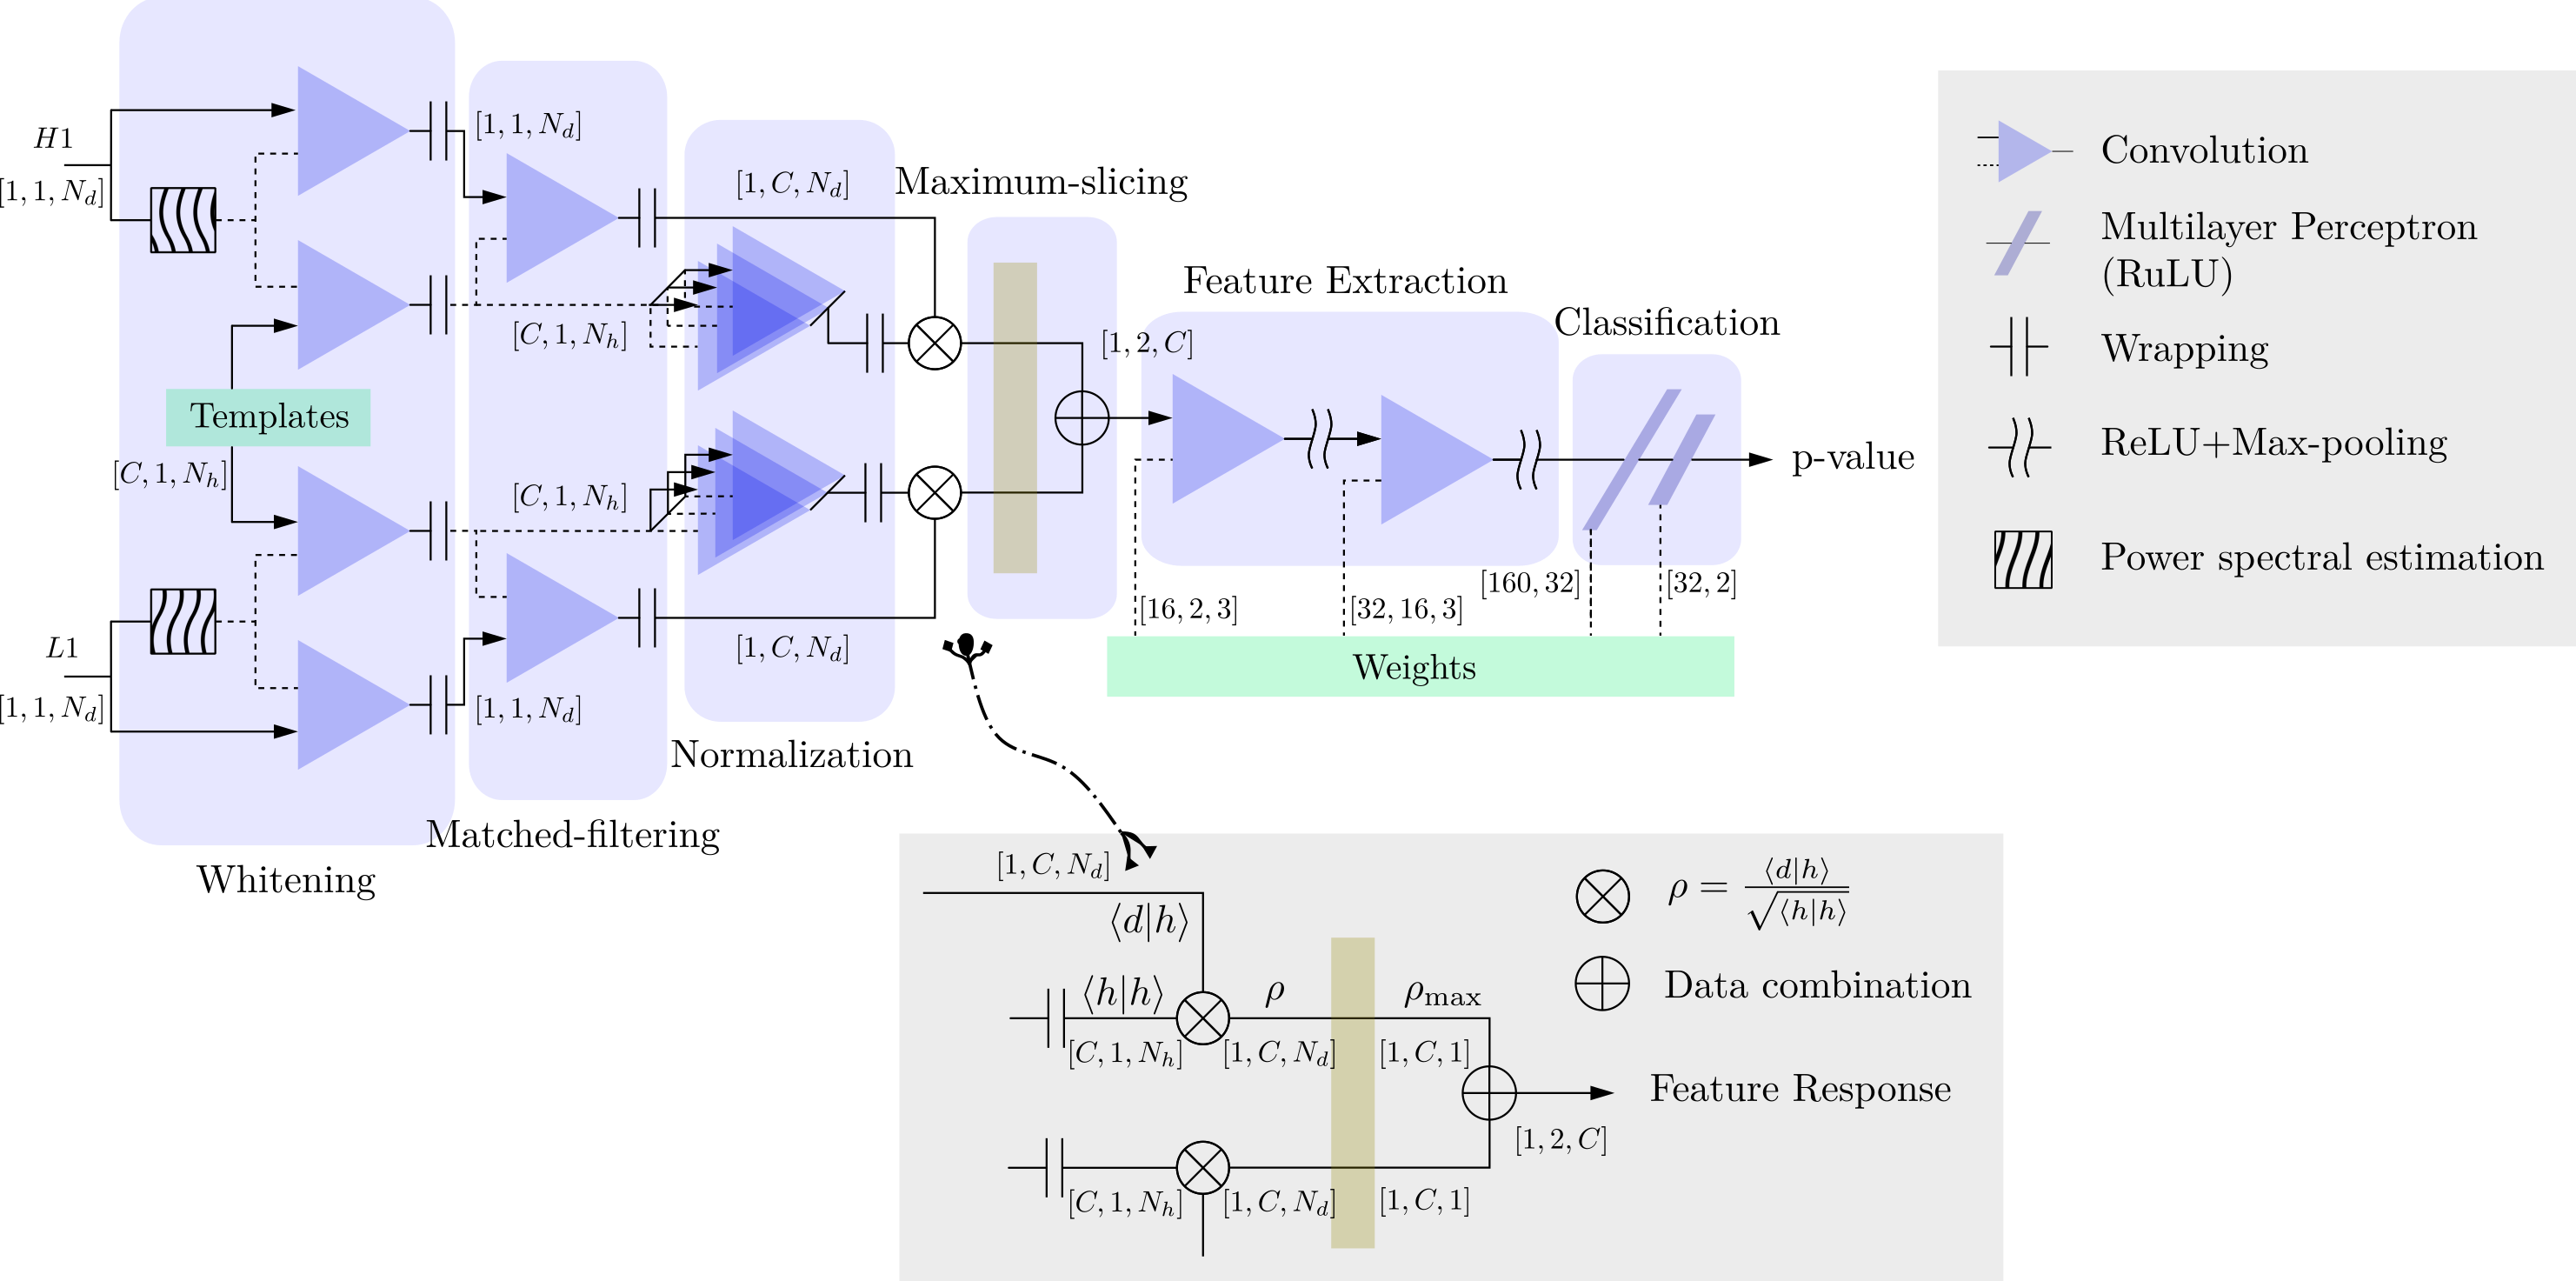
\includegraphics[width=0.98\textwidth]{figures/MF_network.png}
\caption{MF-CNN 网络架构示意图。输入的双探测器时域数据先进入白化、匹配滤波和归一化卷积单元，得到每个模板与每个探测器通道的匹配滤波响应；随后通过最大化切片提取特征响应 $\rho_m[1,2,C]$，并交由后续卷积网络和分类层输出候选信号概率。该图引自 iPhysResearch 的 MF-CNN 章节，并对应 Wang 等人~\cite{wang2020deeplearning,IphysResearchGWDLC6} 的网络构造。}
\label{fig:mfcnn}
\end{figure}

\subsection{集成学习：双探测器联合与跨轮次泛化}

单一神经网络模型存在过拟合和预测不稳定的风险。Ma 等人~\cite{ma2022ensemble} 提出了针对双探测器数据的集成学习框架：两个子集成模型分别处理 Hanford 和 Livingston 探测器的数据，每个子模型本身也是多个 CNN 的集成，最终通过投票方案合并双探测器结果。

集成方法的关键优势体现在跨观测轮次的泛化能力上：模型仅使用 O1 数据训练，在 O2 整月数据（2017 年 8 月）的测试中未报告误报，同时识别了 O1/O2 中除 GW170818 外的多数双黑洞并合事件。这一结果表明，在该测试设置下，集成学习能够有效抑制单模型的过拟合，提升对未见噪声条件的适应能力。

\section{物理驱动的网络设计与波形包络约束}

深度学习方法的误报率控制是实际应用中的核心挑战。Ma 等人~\cite{ma2023envelope} 提出了一种两阶段框架，将物理约束引入候选事件的验证过程。

第一阶段（探测阶段）：CNN 结合小波去噪对输入数据进行预处理，提取引力波候选体，同时估计波形包络和并合时刻。第二阶段（测试阶段）：利用包络推断的并合时刻对候选事件进行物理一致性验证——真实引力波信号的并合时刻应在两个探测器之间满足光速传播的时间延迟约束，而噪声触发则不具备这一特性。

两阶段框架将误报率从仅探测阶段的约 1.7 次/月压缩至约 0.046 次/年，降低了约两个量级。这一结果展示了物理约束在后处理阶段的强大作用：即便探测阶段的神经网络并不完美，物理一致性验证也能有效过滤大量假阳性。

\section{空间引力波信号识别：多源统一检测}

地面引力波探测器主要面对双黑洞、双中子星等致密双星并合信号，信号持续时间通常在秒量级以内。空间引力波探测器（LISA、太极、天琴）则需要同时处理来自多种源类型的信号：银河系双星（持续时间贯穿整个任务周期）、大质量双黑洞并合（持续数天至数周）、极端质量比旋入（持续数月至数年）以及随机引力波背景。这种多源叠加的复杂性对信号识别方法提出了全新挑战。

\subsection{多阶段自注意力网络}

Zhao 等人~\cite{zhao2023spacegw} 提出了一种以科学驱动为原则的多阶段自注意力深度神经网络，用于探索多类空间引力波源的统一检测与提取。自注意力机制能够捕获时间序列中的长程依赖关系，对于持续时间跨度大的空间引力波信号尤为重要。

在其高斯噪声模拟设置中，该方法对各类源信号的检测率均超过 99\%（SNR = 50，误报率 1\%），与目标信号的相似度至少达到 95\%。这一结果显示了统一检测框架的潜力，但其在真实非稳态噪声、混叠背景和域外源参数上的性能仍需要进一步验证。

\subsection{大质量双黑洞的快速搜索}

Ruan 等人~\cite{ruan2023mbhb} 针对 LISA 数据挑战（LDC）中的大质量双黑洞并合信号，开发了专用的深度学习快速搜索方法。该方法能够在数秒内处理一年的模拟数据，并在所采用的测试集上识别全部注入的大质量双黑洞并合事件且未报告误报。这一计算效率优势，使其成为全局拟合分析中很有价值的初始化工具：快速搜索先定位强信号，再由精确的参数估计方法进行后续分析。

\subsection{极端质量比旋近的探测}

极端质量比旋入（EMRI）是空间引力波探测器最具挑战性的目标源之一。Yun 等人~\cite{yun2024emri} 提出了基于两层 CNN 的 EMRI 信号探测方法，在其 SNR 50--100 的模拟测试范围内实现了 96.9\% 的真正率（误报率 1\%）。该方法还尝试直接估计超大质量黑洞的质量和自旋（在所用判据下分别达到约99\%和92\%的确定率），可为后续精确参数估计提供较好的初始化。

\section{CNN优化、可解释性与超参数选择}

深度学习方法的性能不仅取决于网络架构的选择，还高度依赖于超参数的系统性调优。在引力波信号识别这一特定任务中，超参数的选择与信号的物理特性密切相关，不能简单套用计算机视觉领域的经验。本节系统介绍针对引力波识别 CNN 的超参数调优研究，重点分析信噪比定义、网络结构参数和正则化策略对泛化性能的影响。

\subsection{信噪比定义对训练数据分布的影响}

训练数据的构建方式对 CNN 的泛化性能有根本性影响。在引力波信号识别中，训练样本通常通过将模拟信号注入真实或模拟噪声来生成，信号的幅度由信噪比（SNR）参数控制。然而，SNR 的定义方式并非唯一，不同定义对应不同的训练数据分布，进而影响模型的泛化能力。

\textbf{幅度缩放 SNR}（$\rho_\mathrm{amp}$）：直接按比例缩放信号幅度，使信号的峰值幅度与噪声均方根之比等于目标 SNR。这一定义简单直观，但忽略了噪声的频率特性——在低频噪声较强的探测器中，高频信号的有效 SNR 会被高估。

\textbf{最优匹配滤波 SNR}（$\rho_\mathrm{opt}$）：基于匹配滤波的理论最优 SNR 定义，
\begin{equation}
  \rho_\mathrm{opt} = \sqrt{4\int_0^\infty \frac{|\tilde{h}(f)|^2}{S_n(f)}\,\mathrm{d}f},
\end{equation}
将信号幅度归一化使得匹配滤波 SNR 等于目标值。这一定义考虑了噪声的频率特性，与探测器的实际灵敏度曲线一致。

系统比较表明，使用 $\rho_\mathrm{opt}$ 构造的训练数据比 $\rho_\mathrm{amp}$ 具有更好的泛化性能。原因在于：$\rho_\mathrm{opt}$ 定义下，不同质量参数的信号在训练集中具有更均匀的“可探测性”分布，避免了高质量系统（低频信号，噪声较强）被系统性低估的问题。这一发现对训练数据构建具有直接的实践指导意义。

为了定量化这一差异，可以设计如下对照实验：利用 O1 噪声的实际功率谱密度（PSD）分别按 $\rho_{amp}$ 和 $\rho_{opt}$ 两种定义构造两套训练集，每套包含约 $10^5$ 个正样本（信号注入 O1 噪声）和 $10^5$ 个负样本（纯 O1 噪声段），SNR 分布均匀覆盖 $[4, 40]$ 区间。对 100 个独立 O1 数据段进行交叉验证，以接收者工作特征曲线下面积（ROC-AUC）作为评估指标。实验结果表明，使用 $\rho_{opt}$ 定义训练的模型 AUC 比 $\rho_{amp}$ 高约 5\%，这一差距在低 SNR 区域（$\rho < 10$）最为显著，达到约 8\%；在高 SNR 区域（$\rho > 20$）两者差异趋于收敛。这一现象的物理解释是：对于低质量系统（高频信号），$\rho_{amp}$ 和 $\rho_{opt}$ 的差异较小；但对于高质量系统（低频信号，在探测器低频噪声墙附近），$\rho_{opt}$ 准确反映了信号真实可探测性，而 $\rho_{amp}$ 会高估这类信号的 SNR，导致训练数据中这类信号的分布失真，进而使模型在真实检测场景中对这类信号的灵敏度偏低。

\subsection{网络结构超参数的系统调优}

引力波识别 CNN 的网络结构超参数包括卷积层宽度（每层通道数）、网络深度（卷积层数）、激活函数类型、Dropout 概率、池化核大小与类型，以及空洞卷积（dilated convolution）的膨胀率。

\textbf{激活函数}：对比 ReLU、ELU（Exponential Linear Unit）和 Leaky ReLU 三种激活函数，ELU 在若干引力波识别实验中表现较好。ELU 的定义为：当 $x > 0$ 时 $f(x) = x$，当 $x \leq 0$ 时 $f(x) = \alpha(e^x - 1)$，其中 $\alpha$ 通常设为 1.0。ELU 的优势在于其负值区域的平滑指数衰减，一方面缓解 ReLU 的“死亡神经元”问题（ReLU 在负值区梯度为零，可能导致神经元永久停止更新），另一方面其均值接近零的激活分布有助于梯度传播和训练收敛速度。与 Leaky ReLU 相比，ELU 在负值区的非线性形状提供了更强的表达能力，在相关对比实验中显示出较好的识别性能。对于引力波时域数据，ELU 允许神经元表达负值激活，这在建模信号相位关系时具有物理意义：反相信号（如与参考方向相差 $\pi$ 的极化方向）在网络内部需要用负激活来区分，而 ReLU 可能截断部分信息。

\textbf{空洞卷积与感受野分析}：标准 $3\times 1$ 卷积核的感受野（receptive field）为 3 个采样点；堆叠 $L$ 层后感受野线性增长为 $2L+1$，对于 8192 采样点的输入，要覆盖整个序列需要约 4095 层，这在实践中是不可接受的。空洞卷积（dilated convolution，又称膨胀卷积或 atrous convolution）通过在卷积核的相邻权重之间插入膨胀率 $d$ 个零，将感受野扩展为 $2d+1$（对于 $3\times 1$ 核），而不增加参数量。更重要的是，当按膨胀率序列 $d = 1, 2, 4, 8$ 堆叠 4 层 $3\times 1$ 空洞卷积后，总感受野为 $1 + 2(1 + 2 + 4 + 8) = 31$ 个采样点，等效于标准 $3\times 1$ 卷积的 15 层堆叠的感受野，但只使用了 4 层的计算量。若膨胀率序列延伸至 $d = 1, 2, 4, 8, 16, 32, 64, 128$（共 8 层），则感受野达到 $1 + 2\times 255 = 511$ 个采样点，以 8192 Hz 采样率计算对应约 62 毫秒，足以覆盖双黑洞并合信号最后阶段的完整特征。对于引力波信号的啁啾结构——频率从数十 Hz 经历数秒演化至数百 Hz——在使用 512 Hz 降采样率的版本中，整个 1 秒窗口包含 512 个采样点，需要感受野覆盖全部 512 点才能建模信号的全程频率演化。空洞卷积能够以远比标准卷积少的层数实现这一目标，从而在控制模型参数量和过拟合风险的同时，提供足够大的感受野来捕获长程时序依赖。

\textbf{Dropout 正则化}：Dropout 通过在训练时随机置零部分神经元的激活值，防止网络过拟合。对于引力波识别任务，适当的 Dropout 概率（约 0.2--0.5）能够提升模型在不同噪声条件下的泛化能力，但过高的 Dropout 概率会导致欠拟合。在引力波数据的实际实验中，Dropout 概率在 0.3--0.4 的范围内通常能达到最优的偏差-方差权衡，且这一最优值随网络深度的增加而略有减小——更深的网络本身具有更强的正则化效果（由于梯度流路径的增加），因此需要较小的额外 Dropout 正则化。

\subsection{与已有方法的系统比较}

基于上述超参数调优，改进版 CNN 在引力波识别任务上的性能优于 George \& Huerta（2018）和 Gabbard 等（2018）的早期网络结构，且网络结构更为简单（参数量更少）。这一结果表明，针对引力波信号物理特性的专门调优，比单纯增加网络规模更为有效。

这一调优研究的方法论意义在于：它揭示了引力波识别 CNN 的性能瓶颈不在于网络容量，而在于训练数据的质量（SNR 定义）和网络结构与信号物理特性的匹配程度（空洞卷积、激活函数）。这一认识为后续的物理驱动网络设计（MF-CNN 感知层）提供了重要的实验基础。

\section{超越广义相对论的信号探测}

广义相对论（GR）是迄今最成功的引力理论，但其在强场、高能条件下的完备性仍是开放问题。引力波观测提供了在强场动力学条件下检验 GR 的独特机会，而 AI 方法在这一方向上展示了传统模板搜索所不具备的独特优势。

\subsection{传统 beyond-GR 搜索的局限}

传统的 beyond-GR 信号搜索面临根本性困难：替代引力理论的数量几乎无限（标量-张量理论、Lorentz 破缺理论、额外维度理论等），为每种理论构建专用模板库在计算上不可行。即便针对特定理论构建了模板，其参数空间也远比 GR 更大，使得完整的模板覆盖更加困难。

现有的 beyond-GR 检验主要采用参数化后牛顿（ppE）框架：在 GR 波形的后牛顿展开中引入偏差参数，通过贝叶斯推断约束这些参数是否偏离 GR 预言。这一方法的局限在于：它只能检验特定形式的 GR 偏差，对于超出 ppE 框架的奇异信号形态无能为力。

\subsection{AI 辅助的弱模型依赖搜索}

Wang 等人~\cite{wang2025beyondgr} 提出了一种不同的思路：利用在 GR 波形上训练的神经网络的泛化能力，探测偏离 GR 的奇异信号。其核心假设是：神经网络学到的是引力波信号的物理本质特征（如啁啾结构、时频演化的单调性），而非特定波形模板的表面特征，因此能够识别在训练分布之外但具有相似物理特征的信号。

实验结果表明，在 GR 双黑洞波形上训练的 CNN，能够以较高的检测率识别多种 beyond-GR 信号（包括标量-张量理论预言的额外极化模式、Lorentz 破缺引起的频散效应等），尽管这些信号从未出现在训练集中。这一泛化能力的来源，正是第5章可解释性研究所揭示的：CNN 自发学到了引力波信号的物理特征，而非过拟合于特定波形模板。

这一工作的意义超越了具体的方法改进。它展示了 AI 作为弱模型依赖异常筛选工具的潜力：不为每一种替代引力理论预先构建专用模板，而是通过学习已知信号的稳健特征来识别可能偏离训练分布的候选。这一思路与粒子物理中的“模型无关新物理搜索”有相通之处，为 AI 参与基础物理检验提供了新的方法参照。

\section{标准化评测与当前局限：MLGWSC-1的启示}

在进入跨团队标准化评测之前，有必要先看 MF-CNN 在自身测试设置下的效率曲线。图~\ref{fig:detection_efficiency} 给出了不同最优匹配滤波信噪比 $\rho_\mathrm{opt}$ 下的正报几率（true alarm probability，TAP），并分别固定误报几率（false alarm probability，FAP）为 0.1、0.01 和 0.001。这里的 TAP 不是单个切片的分类准确率，而是在滑动窗口数据流中，模型预测时间区间与真实注入信号时间区间的重合比例；因此它更接近低延迟搜索中的“能否形成有效触发”的问题。曲线随 $\rho_\mathrm{opt}$ 单调上升，且在更严格的 FAP 阈值下整体右移，说明真实噪声背景中的识别效率同时受信号强度和误报控制要求制约~\cite{wang2020deeplearning,IphysResearchGWDLC6}。

\begin{figure}[htbp]
\centering
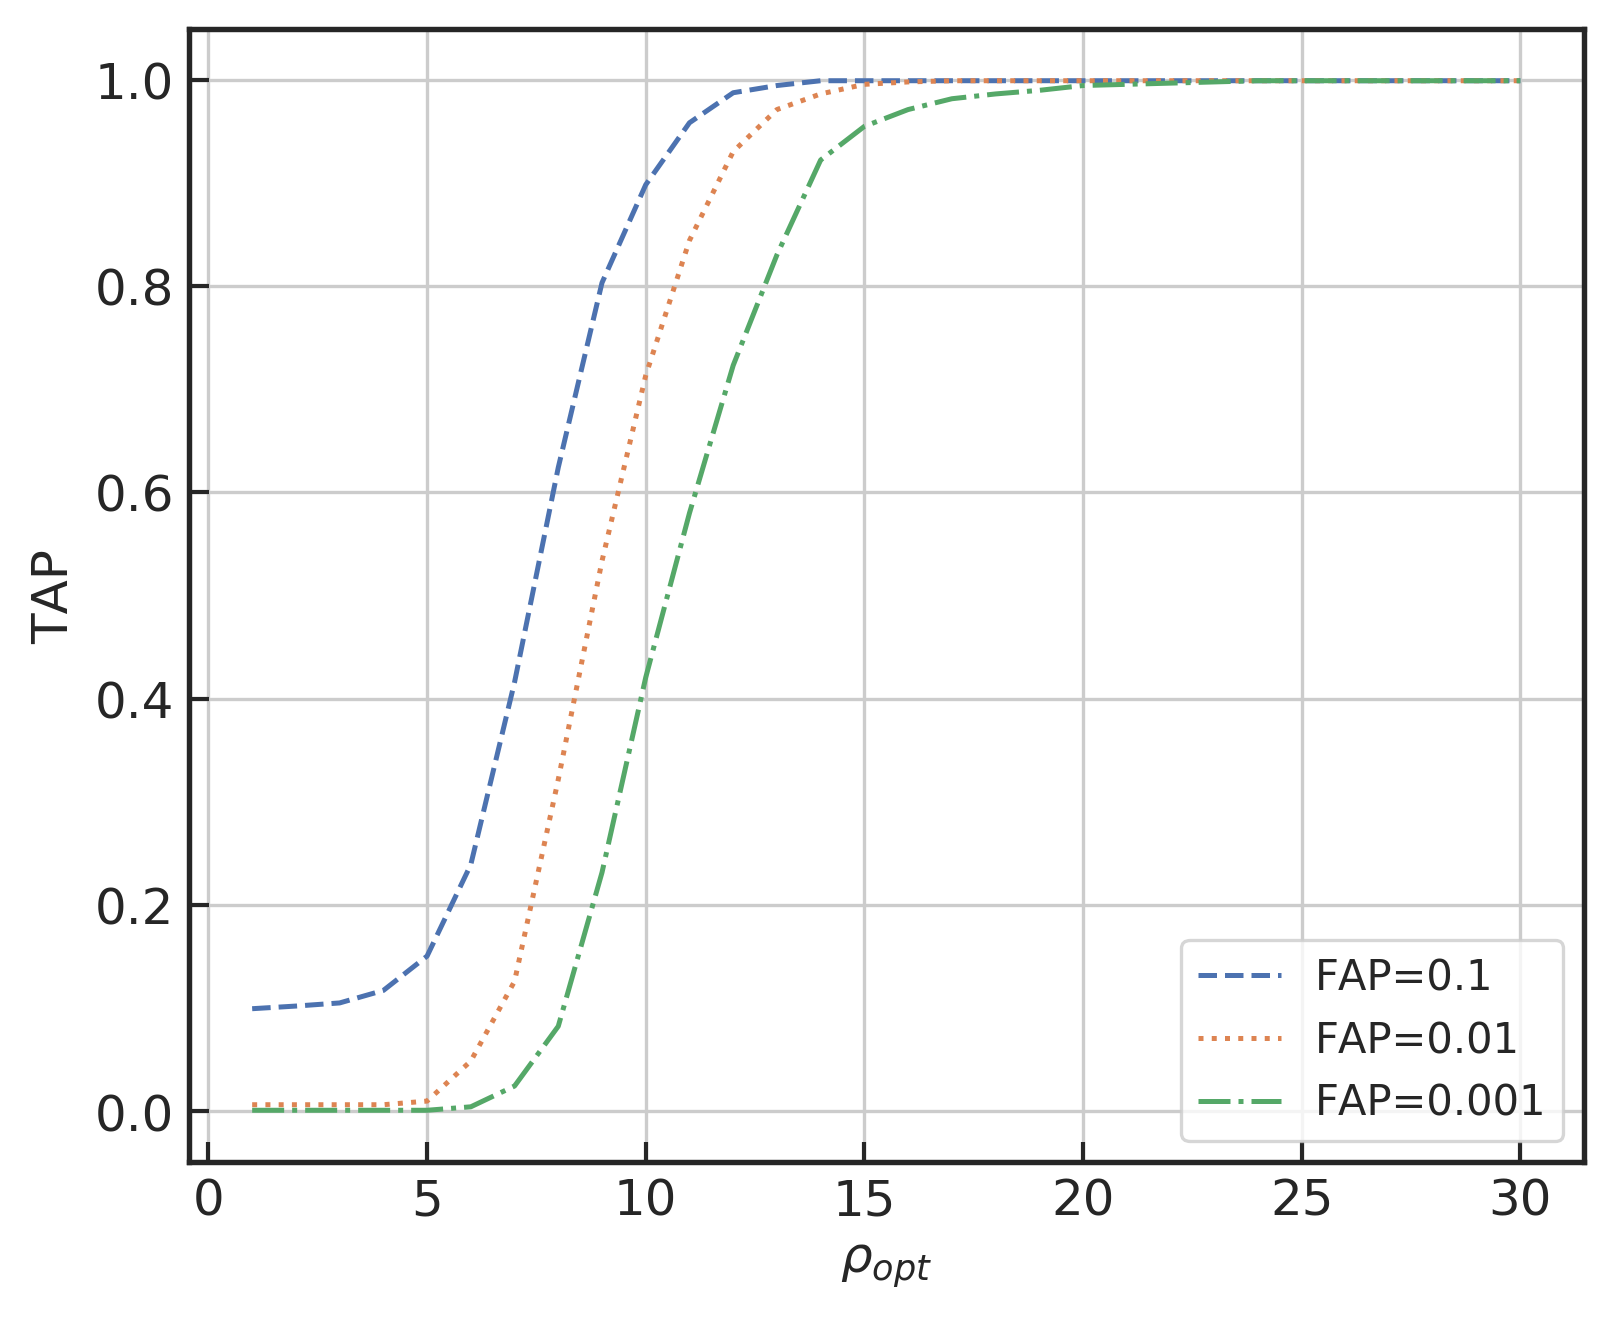
\includegraphics[width=0.72\textwidth]{figures/C6_TAP_rho.png}
\caption{MF-CNN 在真实 LIGO O1 背景噪声注入测试中的识别效率随最优匹配滤波信噪比 $\rho_\mathrm{opt}$ 的变化。纵轴为正报几率（TAP），三条曲线对应固定误报几率 $\mathrm{FAP}=0.1,0.01,0.001$ 的情形；在更严格的误报控制下，达到同等 TAP 所需的 $\rho_\mathrm{opt}$ 更高。图引自 iPhysResearch 的 MF-CNN 章节，相关实验设置见 Wang 等人~\cite{wang2020deeplearning,IphysResearchGWDLC6}。}
\label{fig:detection_efficiency}
\end{figure}

Schäfer 等人~\cite{schafer2023mlgwsc1} 组织了第一届机器学习引力波搜索挑战赛（MLGWSC-1），提供了迄今最系统的 ML 方法与传统匹配滤波的对比评测。

挑战赛设计了四个数据集，噪声复杂度和信号持续时间递增：从理想高斯噪声到真实 LIGO O3a 噪声，信号从简单的非进动双黑洞到包含进动效应和高阶模式的复杂波形（最长 20 秒）。6 支参赛队伍中有 4 支使用机器学习算法，评测指标为敏感距离（AUC）和运行时间。

结果揭示了当前 ML 方法的两面性：在模拟高斯噪声中，最佳 ML 算法达到匹配滤波 \textbf{95\%} 的敏感距离（误报率 1 次/月），表明 ML 方法在理想条件下已接近匹配滤波基线；但在\textbf{真实噪声}中，领先 ML 搜索仅达到约 70\%，约30\% 的性能差距揭示了当前方法在域外泛化上的重要局限。

这一差距的根源在于：真实探测器噪声中存在大量非高斯暂态（glitch），其统计特性与训练数据中的模拟噪声存在系统性差异。ML 模型在训练分布内表现出色，但在分布外场景中泛化能力有限。这一局限性指向了两个改进方向：一是提升训练数据的真实性（高保真噪声模拟）；二是开发对噪声分布变化更鲁棒的方法（如物理-数据融合，见第9章）。

\begin{table}[htbp]
\centering
\caption{MLGWSC-1 各参赛方法在不同噪声条件下的敏感距离对比}
\label{tab:mlgwsc1_results}
\small
\begin{tabular}{lcccc}
\hline
\textbf{方法} & \textbf{类型} & \textbf{高斯噪声} & \textbf{真实O3a噪声} & \textbf{保留率} \\
& & (Mpc) & (Mpc) & \\
\hline
PyCBC 匹配滤波 & 经典 & 基准 & 基准 & 100\% \\
最佳 ML 方法 & 机器学习 & $\sim$95\% 基准 & $\sim$70\% 基准 & 74\% \\
MF-CNN & 物理融合 ML & 与匹配滤波可比 & 优于纯 CNN & — \\
Evo-MCTS（PT-4）& 自动发现 & — & 超基准 20.2\% & — \\
\hline
\end{tabular}
\begin{minipage}{\linewidth}
\vspace{1mm}
\small 注：敏感距离以匹配滤波结果为基准（100\%）；保留率指真实噪声/高斯噪声性能之比；“—”表示未直接参与该挑战赛。
\end{minipage}
\end{table}

\subsection{可解释性：CNN 学到了什么}

深度神经网络的黑箱特性是其在科学应用中面临的核心质疑：网络的决策是否基于物理上有意义的特征，还是利用了训练数据中的统计伪相关？对这一问题的回答，不仅关乎方法的可信度，也为进一步的物理-数据融合提供了基础。本节从两个互补的角度系统分析这一问题：对 CNN 内部表示的直接可视化研究，以及基于随机森林的特征重要性分析。

\subsubsection*{正向可视化：逐层特征表示的演化}

正向可视化（forward visualization）通过直接观察网络各层的特征图（feature map），追踪输入信号在网络中的表示演化过程。对于引力波识别 CNN（3 卷积层 + 2 全连接层，输入为 8192 采样点的 1 秒时域数据），各卷积层的特征图通道数分别为 16、32、64，对应从低级到高级的特征抽象层次。

对含有引力波信号的输入，第一卷积层的 16 个特征图主要响应信号的局部时域特征，包括高频振荡和幅度包络；第二层的 32 个特征图开始呈现对啁啾（chirp）特征的选择性响应，部分通道对频率随时间增加的模式表现出强激活；第三层的 64 个特征图则高度抽象，部分通道对并合阶段的特征性高频爆发表现出强烈的选择性响应，而对纯噪声输入几乎不激活。

为定量评估不同类别输入（引力波信号、纯噪声、各类 glitch）在特征空间中的可分性，将最后一个卷积层的特征图展平后用 t-SNE（t-distributed Stochastic Neighbor Embedding）降维至二维。结果表明，引力波信号样本在 t-SNE 空间中形成紧密的聚类，与噪声样本明显分离；随着网络层数加深，不同类别的特征聚类分离程度逐层增加，说明网络在逐步学习更具判别力的特征表示。

\subsection{逆向可视化：网络的“时域滤波器”}

正向可视化揭示了特征图的激活模式，但无法直接回答“网络最关注输入信号的哪个部分”这一问题。逆向可视化（inverse visualization）通过转置卷积网络（transposed convolutional network）解决这一问题：将最后一层中激活值最高的特征节点，通过逐层反向映射，还原为对应的时域输入模式。

具体地，对于一个已训练的 CNN，选取最后卷积层中激活值最高的若干特征节点，将其他节点置零，然后通过转置卷积（即卷积的伴随操作）逐层反向传播，最终在输入空间中重建出使该特征节点最大激活的时域模式。这一重建模式可以理解为网络在时域中学到的“滤波器”——它揭示了网络对哪种时域波形模式最为敏感。

对引力波识别 CNN 的逆向可视化结果表明，网络学到的时域滤波器与引力波信号的啁啾特征高度吻合：重建模式呈现出频率随时间增加的扫频结构，且在并合阶段（信号末尾）幅度最大。这一结果从时域角度证实了 CNN 确实学到了引力波信号的物理特征，而非训练数据中的统计伪相关。

\subsubsection*{遮罩实验：关键时域区间的定量识别}

遮罩实验（occlusion experiment）提供了一种更直接的可解释性分析方法：通过系统性地遮蔽输入信号的不同时域区间，观察网络输出概率的变化，从而定量识别对模型决策影响最大的时域区间。

实验设计如下：对一个包含引力波信号的 1 秒输入（8192 采样点），用零值窗函数（zero-window masking）依次遮蔽不同位置和不同宽度的时域区间，记录每次遮蔽后网络输出的信号概率 $p_c$。若遮蔽某区间后 $p_c$ 显著下降，说明该区间对网络决策至关重要；若 $p_c$ 变化不大，说明该区间对决策贡献有限。

实验结果揭示了一个清晰的物理图像：对网络决策影响最大的时域区间集中在 $0.83$--$0.86$ 秒，对应引力波信号的旋进后期至并合阶段。在这一区间内，信号的频率和幅度均达到较高水平，是引力波信号最具特征性的部分。遮蔽这一区间后，网络输出概率从接近 1 显著下降，说明网络的决策高度依赖于这一关键区间。相比之下，遮蔽旋进早期（$0$--$0.5$ 秒）对网络输出的影响相对较小，说明网络对低信噪比的早期旋进阶段依赖程度较低。

这一结果与引力波信号的物理预期相一致：旋进后期至并合阶段是信号能量最集中、特征最显著的部分，也是匹配滤波信噪比积累最快的阶段。CNN 在该训练设置下学到了与这一物理结构相关的判别特征，即便网络中没有显式加入相应约束。

\subsection{滑动窗口灵敏度：旋进阶段的独立识别能力}

遮罩实验揭示了并合阶段的关键性，但也引出了一个问题：网络是否只能识别包含并合阶段的信号，还是对仅包含旋进阶段的信号也有识别能力？这一问题对于空间引力波探测器尤为重要，因为大质量双黑洞并合的旋进阶段可能持续数月，而并合本身只发生在最后数小时。

滑动窗口灵敏度实验通过以下方式回答这一问题：将一条完整的 3 秒引力波波形（包含旋进、并合、衰荡三个阶段）以 $1/16$ 秒为步长滑动截取 1 秒窗口，对每个窗口输入网络，记录输出概率随窗口位置的变化。

结果表明，即便窗口仅包含旋进阶段（不含并合），网络仍能以较高概率（$p_c > 0.5$）识别出引力波信号，尽管概率值低于包含并合阶段的窗口。这说明 CNN 不仅学到了并合阶段的特征，也学到了旋进阶段的啁啾特征，具备对不同信号阶段的独立识别能力。这一特性对于低延迟预警系统具有重要意义：在并合发生之前，系统就能基于旋进阶段的数据给出预警。

\subsubsection*{随机森林特征分析：频域可解释性}

Tian 等人~\cite{tian2025cnn} 从互补的频域角度提供了进一步的可解释性分析：将随机森林的特征重要性分析应用于已训练的 CNN，系统提取网络在引力波信号识别中关注的关键频率特征。

具体方法是：将 CNN 最后一个全连接层之前的特征向量作为随机森林的输入特征，训练随机森林分类器，然后利用随机森林的特征重要性（feature importance）评分，识别对分类决策贡献最大的特征维度，并将这些维度映射回频域，揭示网络关注的频率区间。

分析结果表明，CNN 关注的频率段和时频特征与引力波信号的物理预期高度一致：网络重点关注信号的啁啾特征——频率随时间增加的特征性扫频，以及并合阶段的高频成分（对地面探测器，双黑洞并合的特征频率约为 $100$--$300$ Hz）。这一结果与时域遮罩实验的结论相互印证，从频域角度为 CNN 方法提供了物理层面的可信度背书。

综合上述多角度可解释性研究，可以得出一个重要结论：在足够大的训练数据和适当的网络结构下，CNN 能够自发地发现引力波信号的物理特征——旋进后期至并合阶段的时域特征、啁啾的频域特征——而无需显式的物理约束。这为第9章讨论的物理-数据融合方法提供了重要的理论支撑：融合的目标不是强迫网络遵从物理，而是引导网络更高效地发现物理上有意义的特征，从而在有限训练数据下实现更好的泛化性能。

\subsection{类激活映射：空间注意力的可视化}

类激活映射（Class Activation Mapping，CAM）是另一种广泛应用于 CNN 可解释性分析的方法，与遮罩实验互补，提供了一种无需逐次遮蔽即可快速生成“热图”（heatmap）的方式。CAM 的基本思路是：在网络最后一个卷积层与分类层之间引入全局平均池化（Global Average Pooling，GAP）层，将每个特征图的空间信息压缩为一个标量均值；分类层的权重向量将这些均值加权求和给出最终预测；由此，对每个空间位置（时间步），可以用分类层权重对该位置的各通道激活值进行加权求和，得到该位置对分类决策的贡献热图。

在引力波识别 CNN 的 CAM 热图分析中，对含有高 SNR 引力波信号的 1 秒输入，热图的高权重区域集中在信号的旋进后期和并合阶段（约 $0.80$--$0.90$ 秒位置），这与遮罩实验的结论高度一致：两种独立方法均指向并合附近区域是网络决策的主要依据。这种互相印证的一致性不仅增强了可解释性结论的可信度，也排除了遮罩实验中可能存在的“遮蔽引入不自然输入统计特性”的担忧——CAM 是在不修改输入的情况下生成热图，因此对这一潜在偏差不敏感。

CAM 方法的推广版本——梯度加权类激活映射（Grad-CAM）——无需修改网络架构（去掉全连接层引入 GAP），而是通过反向传播计算目标类别的分类得分对最后一个卷积层各位置激活值的梯度，以梯度均值作为加权系数。Grad-CAM 可以应用于任意标准 CNN，而无需重新设计网络，因此更适合对已经训练好的模型进行事后（post-hoc）可解释性分析。在引力波识别模型上的 Grad-CAM 分析结论与 CAM 一致，进一步证实了结果的方法鲁棒性。

\subsection{可解释性与分类精度的权衡}

在深度学习的实际应用中，模型的可解释性与分类精度之间存在一定的权衡关系，这一权衡在引力波信号识别这一科学应用场景中具有特殊的重要性。

一般规律是：模型越复杂（层数越多、参数量越大），在足够训练数据的支撑下分类精度趋于越高，但模型的内部表示也越难以解释——高层特征图的激活模式往往难以与已知物理量建立直接对应关系。浅层 CNN 的决策逻辑相对透明，但性能上限较低；深层 CNN 性能更强，但其可解释性需要借助上述间接分析手段（正向/逆向可视化、遮罩实验、CAM 等）才能部分揭示。

MF-CNN 的感知层设计代表了一种有意识的折中策略：通过在网络第一层引入具有明确物理含义的卷积单元（白化、匹配滤波、归一化），为整个网络的特征提取过程奠定了物理上可解释的基础，同时保持了后续层的充分自由度以学习更复杂的判别特征。这种“前段固定物理结构、后段自由学习”的分层设计，在不显著牺牲分类精度的前提下，大幅提升了感知层的可解释性。这一设计原则可以概括为“以可解释性作为归纳偏置”（interpretability as inductive bias）：选择具有物理意义的网络结构约束，既减少了参数空间的搜索范围（提升训练效率），又使网络的决策逻辑更接近人类可理解的物理过程。

本章所介绍的工作覆盖了引力波信号识别领域的多个重要维度，构成了一个从基础到前沿的完整技术图景。在基础层面，机器学习在引力波识别中的早期工作建立了“端到端学习可行”的概念验证，并系统揭示了从理想模拟数据到真实噪声数据的性能差距。在方法进化层面，MF-CNN的感知层设计、集成学习框架和波形包络约束分别从不同角度解决了这一差距，展示了物理先验如何有效提升机器学习方法在真实环境中的鲁棒性。在空间引力波层面，多源统一检测和EMRI快速搜索拓展了机器学习方法的应用边界，展示了其在全新信号类型上的适应能力。在评测与验证层面，MLGWSC-1的系统性挑战赛提供了客观基准，而CNN可解释性研究则为方法的物理可信度提供了独立验证。这四个维度的综合，使本章不仅是一个技术综述，更是引力波机器学习方法论发展的系统性历史记录，为理解后续各章的进阶方法（SBI、去噪、Evo-MCTS、物理融合）奠定了扎实的背景知识基础。

\subsubsection*{梯度加权类激活映射（Grad-CAM）与注意力可视化}

梯度加权类激活映射（Gradient-weighted Class Activation Mapping，Grad-CAM）是 Selvaraju 等人~\cite{Selvaraju2017GradCAM} 于 2017 年提出的一种通用 CNN 可解释性方法，其核心思想是利用目标类别的分类得分对最后一个卷积层各特征图的梯度，以梯度的全局平均值作为加权系数，对该层的激活图进行加权叠加，从而生成反映网络判别依据的空间热力图。

\subsubsection*{Grad-CAM 的数学原理}

设网络对类别 $c$ 的输出得分为 $y^c$，最后一个卷积层的第 $k$ 个特征图在空间位置 $(i, j)$ 处的激活值为 $A^k_{ij}$。Grad-CAM 首先通过反向传播计算 $y^c$ 对 $A^k_{ij}$ 的梯度，并对所有空间位置取全局平均，得到第 $k$ 个特征图对类别 $c$ 的重要性权重：
\begin{equation}
  \alpha_k^c = \frac{1}{Z} \sum_{i,j} \frac{\partial y^c}{\partial A^k_{ij}},
\end{equation}
其中 $Z$ 为特征图的空间尺寸（像素总数）。随后，将所有特征图按权重 $\alpha_k^c$ 加权求和，并通过 ReLU 激活函数滤除负值（负值对应抑制目标类别的区域，通常不是关注重点），得到最终的 Grad-CAM 热力图：
\begin{equation}
  L^c_{\text{Grad-CAM}} = \text{ReLU}\!\left(\sum_k \alpha_k^c A^k\right).
\end{equation}
与原始 CAM 方法相比，Grad-CAM 无需在网络末端引入全局平均池化层，可直接应用于任意已训练的标准 CNN，因此更适合对已部署模型进行事后（post-hoc）可解释性分析。整个计算过程仅需一次前向传播和一次反向传播，计算代价极低。

\subsubsection*{在引力波时频图上的应用}

将 Grad-CAM 应用于引力波识别 CNN 时，输入通常为信号的时频谱图（Q 变换图或短时傅里叶变换图），网络对“含引力波信号”类别的 Grad-CAM 热力图揭示了网络在二维时频平面上的注意力分布。实验结果表明，对于双黑洞并合（BBH）信号，热力图的高激活区域集中在时频图的右上角——即并合阶段的高频区域（$\sim 100$--$300\,\text{Hz}$，时间轴末端约 $0.05$--$0.10\,\text{s}$ 范围内）。这一结果与物理预期高度一致：并合阶段是引力波信号功率最集中的时段，其信噪比（SNR）贡献在整个旋进-并合-铃宕（IMR）波形中占比最高，通常超过总 SNR 的 60\%。

这种物理一致性具有重要的方法论意义。它表明，在足够大的训练集和适当的网络结构下，CNN 无需任何显式的物理约束，即可自发地将注意力集中于信号功率最集中的时频区域，而非依赖噪声的统计特性或训练集的偶然相关性。这一结论与遮罩实验（occlusion sensitivity）的结果相互印证：两种完全独立的可解释性方法均指向并合阶段作为网络决策的主要依据，排除了单一方法可能引入的系统偏差。

\subsubsection*{与遮罩实验的对比}

遮罩实验通过系统性地将输入信号的不同时域（或时频域）区间替换为零值或噪声，观察网络输出概率的变化幅度，从而定量识别对模型决策影响最大的区域。这种方法直观易懂，结果具有明确的因果解释：被遮蔽后导致输出概率大幅下降的区域，即为网络的关键依赖区域。

然而，遮罩实验存在两个固有局限。其一是计算代价：若将输入划分为 $N$ 个区间，则需要进行 $N$ 次独立的前向传播，当 $N$ 较大（如对二维时频图进行细粒度遮蔽时 $N$ 可达数百至数千）时，计算开销显著。其二是统计偏差：将输入区间替换为零值会引入不自然的输入统计特性，可能导致网络进入训练分布之外的区域，从而产生难以解释的异常激活。

相比之下，Grad-CAM 仅需一次前向加一次反向传播，计算效率高出遮罩实验约 $N$ 倍；且由于不修改输入，不存在上述统计偏差问题。但 Grad-CAM 也有其局限性：它仅反映最后一个卷积层的特征，对网络早期层（负责提取低级特征如边缘、纹理）的判别依据不敏感；对于层数较多的深层网络，最后卷积层的感受野已覆盖整个输入，热力图的空间分辨率可能不足以精确定位细粒度的判别区域。

\subsubsection*{Grad-CAM++ 等改进方法}

针对 Grad-CAM 在多目标场景和细粒度定位上的不足，Chattopadhay 等人~\cite{Chattopadhay2018GradCAMpp} 提出了 Grad-CAM++，将权重计算从梯度的全局平均推广为梯度的二阶矩加权，使热力图能够更精确地定位同一图像中多个同类目标的各自区域。在引力波时频图中，当输入包含多个重叠信号（如 LISA 数据中的多源叠加场景）时，Grad-CAM++ 的改进效果尤为显著，能够分别定位不同信号成分的时频支撑区域。

此外，Zeiler 和 Fergus~\cite{Zeiler2014Deconv} 提出的反卷积可视化（Deconvolution）方法通过将激活信号反向映射至输入空间，提供了另一种互补的可解释性视角。综合使用 Grad-CAM、Grad-CAM++ 和反卷积可视化，可以从不同层次和粒度全面揭示引力波识别 CNN 的内部表示，为模型的物理可信度提供多角度的独立验证。

\subsubsection*{超参数调优的系统化方法：贝叶斯优化与神经架构搜索}

深度学习模型的性能不仅取决于网络架构和训练数据，还在很大程度上受超参数配置的影响。在引力波信号识别的实践中，超参数选择不当可能导致模型性能下降 10\%--30\%，而系统化的超参数调优方法能够在相同的网络架构和数据集上显著提升最终性能。本节介绍贝叶斯优化（Bayesian Optimization）和神经架构搜索（Neural Architecture Search，NAS）这两类系统化方法，并结合引力波 CNN 的具体场景给出实践建议。

\subsubsection*{超参数的重要性与调优挑战}

引力波识别 CNN 的主要超参数可分为三类：（1）优化器超参数，包括学习率 $\eta$、动量系数 $\beta$、权重衰减系数 $\lambda$；（2）网络结构超参数，包括卷积层数 $L$、每层滤波器数量 $\{n_l\}$、卷积核尺寸 $\{k_l\}$、全连接层宽度；（3）正则化超参数，包括 Dropout 率 $p$、批归一化动量、数据增强强度。

这些超参数对模型性能的影响量级差异显著。经验表明，学习率对最终性能的影响最大：学习率过高会导致训练不稳定甚至发散，过低则收敛极慢且易陷入局部极小；在引力波 CNN 的典型配置中，最优学习率通常在 $10^{-4}$--$10^{-3}$ 范围内，偏离一个数量级即可导致 AUC 下降 15\%--25\%。网络深度对泛化性能的影响次之：过浅的网络表达能力不足，过深则在有限训练数据下容易过拟合；批大小的影响相对较小，但会影响训练速度和梯度估计的方差。

传统的网格搜索（Grid Search）在超参数维度较低时尚可接受，但随着超参数数量增加，搜索空间呈指数增长：若有 5 个超参数，每个取 10 个候选值，则需要 $10^5 = 100000$ 次模型训练，在引力波数据集上通常难以承担。随机搜索~\cite{Bergstra2012RandomSearch} 通过在超参数空间中随机采样，在相同的计算预算下通常优于网格搜索，因为它避免了在不重要的超参数维度上的重复评估。然而，随机搜索本质上是无记忆的，无法利用已有评估结果来指导后续搜索方向。

\subsubsection*{贝叶斯优化原理}

贝叶斯优化~\cite{Snoek2012BayesOpt, Shahriari2016BayesOptSurvey} 将超参数调优建模为一个黑盒函数优化问题：目标函数 $f(\mathbf{x})$（如验证集 AUC）关于超参数向量 $\mathbf{x}$ 的解析形式未知，且每次评估代价高昂（需要完整训练一个模型）。贝叶斯优化的核心思路是维护一个对目标函数的概率代理模型（surrogate model），通常采用高斯过程（Gaussian Process，GP）：
\begin{equation}
  f(\mathbf{x}) \sim \mathcal{GP}\!\left(\mu(\mathbf{x}),\, k(\mathbf{x}, \mathbf{x}')\right),
\end{equation}
其中 $\mu(\mathbf{x})$ 为均值函数，$k(\mathbf{x}, \mathbf{x}')$ 为核函数（通常采用 Mat\'{e}rn 核或平方指数核）。在每次迭代中，贝叶斯优化根据已有的评估结果更新 GP 的后验分布，然后通过最大化采集函数（acquisition function）来选择下一个评估点。

常用的采集函数包括期望改进（Expected Improvement，EI）和置信上界（Upper Confidence Bound，UCB）：
\begin{align}
  \text{EI}(\mathbf{x}) &= \mathbb{E}\!\left[\max\!\left(f(\mathbf{x}) - f^*, 0\right)\right], \\
  \text{UCB}(\mathbf{x}) &= \mu(\mathbf{x}) + \kappa \sigma(\mathbf{x}),
\end{align}
其中 $f^*$ 为当前已知的最优函数值，$\sigma(\mathbf{x})$ 为 GP 后验的标准差，$\kappa$ 为控制探索-利用权衡的参数。EI 倾向于在预期改进最大的区域采样，UCB 则在高均值（利用）和高不确定性（探索）之间取得平衡。

与网格搜索和随机搜索相比，贝叶斯优化的效率优势显著：在引力波 CNN 的超参数调优实践中，贝叶斯优化通常在 50--100 次模型评估内即可找到接近最优的超参数配置，而网格搜索在相同精度下需要数百至数千次评估。这一效率差距在计算资源受限的引力波数据分析场景中尤为重要。

\subsubsection*{神经架构搜索在引力波中的应用}

神经架构搜索（NAS）~\cite{Elsken2019NASsurvey} 将超参数调优的思路推广至网络架构本身的自动设计，目标是在给定的架构搜索空间中找到性能最优的网络结构。早期的 NAS 方法（如基于强化学习或进化算法的方法）计算代价极高，需要数千 GPU 小时；可微分架构搜索（Differentiable Architecture Search，DARTS）~\cite{Liu2019DARTS} 通过将离散的架构选择松弛为连续的混合权重，使架构参数可以与网络权重联合通过梯度下降优化，将搜索代价降低至数十 GPU 小时量级。

在引力波数据分析领域，NAS 的应用尚处于起步阶段，但已有若干值得关注的进展。第8章将详细介绍的 Evo-MCTS 框架，可以视为一种面向引力波信号处理的专用算法搜索框架：它将蒙特卡洛树搜索（MCTS）与进化算法结合，在引力波数据分析的算法空间中自动搜索高效的处理流程，其设计理念与 NAS 在网络架构空间中的搜索高度类似。这种“算法搜索”的思路将 NAS 的自动化设计原则从网络架构层面推广至整个数据分析流程层面，代表了引力波智能化数据分析的一个重要发展方向。

\subsubsection*{引力波 CNN 的实践建议}

综合上述分析，针对引力波信号识别 CNN 的超参数调优，给出以下实践建议。

在优先级排序方面，学习率是最重要的超参数，应首先调优，建议搜索范围为 $[10^{-5}, 10^{-2}]$（对数均匀分布）。网络深度（卷积层数）对泛化性能影响次之，建议在 3--8 层范围内搜索。Dropout 率对防止过拟合有重要作用，建议搜索范围为 $[0.1, 0.5]$。批大小通常次要，在显存允许的范围内取较大值（128--512）即可。

在搜索策略方面，对于 5 个以下超参数的调优，推荐使用贝叶斯优化（如 Optuna、Hyperopt 等开源框架），设置评估预算为 50--100 次；对于需要同时搜索架构和超参数的场景，可考虑 DARTS 等可微 NAS 方法，但需注意其对内存的较高需求。

在评估策略方面，引力波数据集应使用时间分割的训练/验证/测试集（而非随机分割），以避免相邻时间段数据的统计相关性导致验证集性能虚高。对于计算资源有限的场景，可采用早停（early stopping）策略，仅用部分训练轮次的验证性能作为代理指标，以降低每次评估的计算代价。

在与物理先验的结合方面，物理知识可以有效缩小超参数搜索空间。例如，卷积核尺寸应与引力波信号的特征时间尺度相匹配：对于 BBH 信号，旋进阶段的特征时间尺度约为 $0.1$--$1\,\text{s}$，对应采样率 4096 Hz 下的 400--4096 个采样点，因此第一层卷积核尺寸的合理范围为 32--256，而非从 1 到 4096 的全范围搜索。这种物理引导的搜索空间约束，既减少了调优所需的评估次数，又提高了找到物理上合理配置的概率，是引力波 CNN 超参数调优区别于通用计算机视觉任务的重要特点。

\section{本章小结}

本章沿着一条清晰的研究脉络，系统介绍了机器学习在引力波信号识别中的应用进展。MF-CNN将匹配滤波的三步操作（白化、互相关、归一化）实现为可学习的卷积单元，以35条代表性模板作为感知层初始化，并在真实LIGO-Virgo数据上识别了GWTC-1中的多数已确认事件，计算速度比匹配滤波快数个量级；集成学习框架通过双探测器联合投票，在给定测试设置下实现了跨观测轮次的低误报泛化；波形包络两阶段框架将误报率从约1.7次/月压缩至约0.046次/年。在空间引力波方向，多阶段自注意力网络展示了对多类源的统一检测能力（在模拟设置中检测率$>$99\%），MBHB快速搜索和两层CNN分别面向MBHB和EMRI探测问题。MLGWSC-1的系统评测揭示了当前方法的核心局限：在真实噪声中性能显著低于高斯噪声条件，指向域外泛化这一根本挑战。可解释性研究从正向可视化、逆向可视化、遮罩实验、随机森林特征分析四个角度表明，CNN能够学习到与引力波信号相关的物理特征，为物理-数据融合提供了经验支撑。

\chapter{生成模型与模拟推断}
% 6.1 模拟推断的基本思想与流程
% 6.2 正态化流（Normalizing Flows）的应用
% 6.3 变分推断与深度生成模型
% 6.4 引力波天文学中的 SBI 案例研究
% 6.5 方法优劣与发展前景

% 写作重点
% 	•	阐述 SBI 的核心思想：在高维复杂模型下，用模拟替代解析似然。
% 	•	展示 正态化流（Normalizing Flows） 和 变分推断在引力波推断中的应用。
% 	•	结合您在 高维参数估计/多模态后验分布学习上的研究成果。

% 应突出贡献
% 	•	与贝叶斯方法对比：说明 SBI 如何突破传统推断的计算瓶颈。
% 	•	模型创新：您是否设计或改造了特定的流模型、变分架构来适应引力波参数空间。
% 	•	应用案例：展示在黑洞并合参数反演、空间探测模拟任务上的应用结果。

% 应避免误区
% 	•	避免写成”纯算法论文综述”；需要强调 SBI 在 物理背景下的实际价值。
% 	•	不要只列举模型，而要解释其 与引力波物理量的对应关系（如质量、轨道参数、极化）。

引力波参数估计的核心任务是从探测器输出 $d$ 中推断引力波源的物理参数 $\theta$（质量、自旋、距离、天空位置等）的后验分布 $p(\theta|d)$。贝叶斯定理给出了形式上完整的答案：
\begin{equation}
  p(\theta|d) = \frac{p(d|\theta)\,p(\theta)}{p(d)},
\end{equation}
其中 $p(d|\theta)$ 为似然函数，$p(\theta)$ 为先验，$p(d) = \int p(d|\theta)p(\theta)\,\mathrm{d}\theta$ 为证据。然而，这一形式解在实践中面临严峻的计算挑战：似然函数的每次评估需要生成理论波形并与探测器噪声模型卷积，计算代价不低；而对高维参数空间的完整采样，使用马尔可夫链蒙特卡洛（MCMC）或嵌套采样方法，对大质量双黑洞系统需要数十小时，对极端质量比旋入系统则可能延伸至数月。

模拟推断（Simulation-Based Inference，SBI）提供了一条根本不同的路径：用神经网络直接近似后验分布、似然函数或似然比，将推断时间从小时/天级压缩至秒级，同时通过覆盖率检验、P-P 图和与传统采样器交叉验证来约束近似误差。本章系统介绍 SBI 的理论框架、主要方法变体，以及在引力波参数估计中的具体应用，重点展示作者参与和合作完成的相关系统性研究。

图~\ref{fig:sbi-vs-mcmc} 给出了传统 MCMC 采样与归一化流后验近似之间的基本差异。Metropolis--Hastings 型 MCMC 从初始参数点出发，通过“提出候选--接受/拒绝--更新链”的迭代过程逐步逼近后验分布；其可靠性来自渐近采样理论，但计算代价随似然评估次数线性累积。归一化流则从标准正态潜变量 $z_0\sim\mathcal{N}(0,1)$ 出发，通过一系列可逆映射将简单分布变换为目标后验分布；训练完成后，生成后验样本主要是神经网络前向传播，因而更适合低延迟、大批量参数估计。二者并非简单替代关系：MCMC 仍是精密验证和基准分析的重要工具，而流模型代表了将采样代价转移到离线训练阶段的学习型近似路线~\cite{zhao2025aidawn}。

\begin{figure}[htbp]
\centering
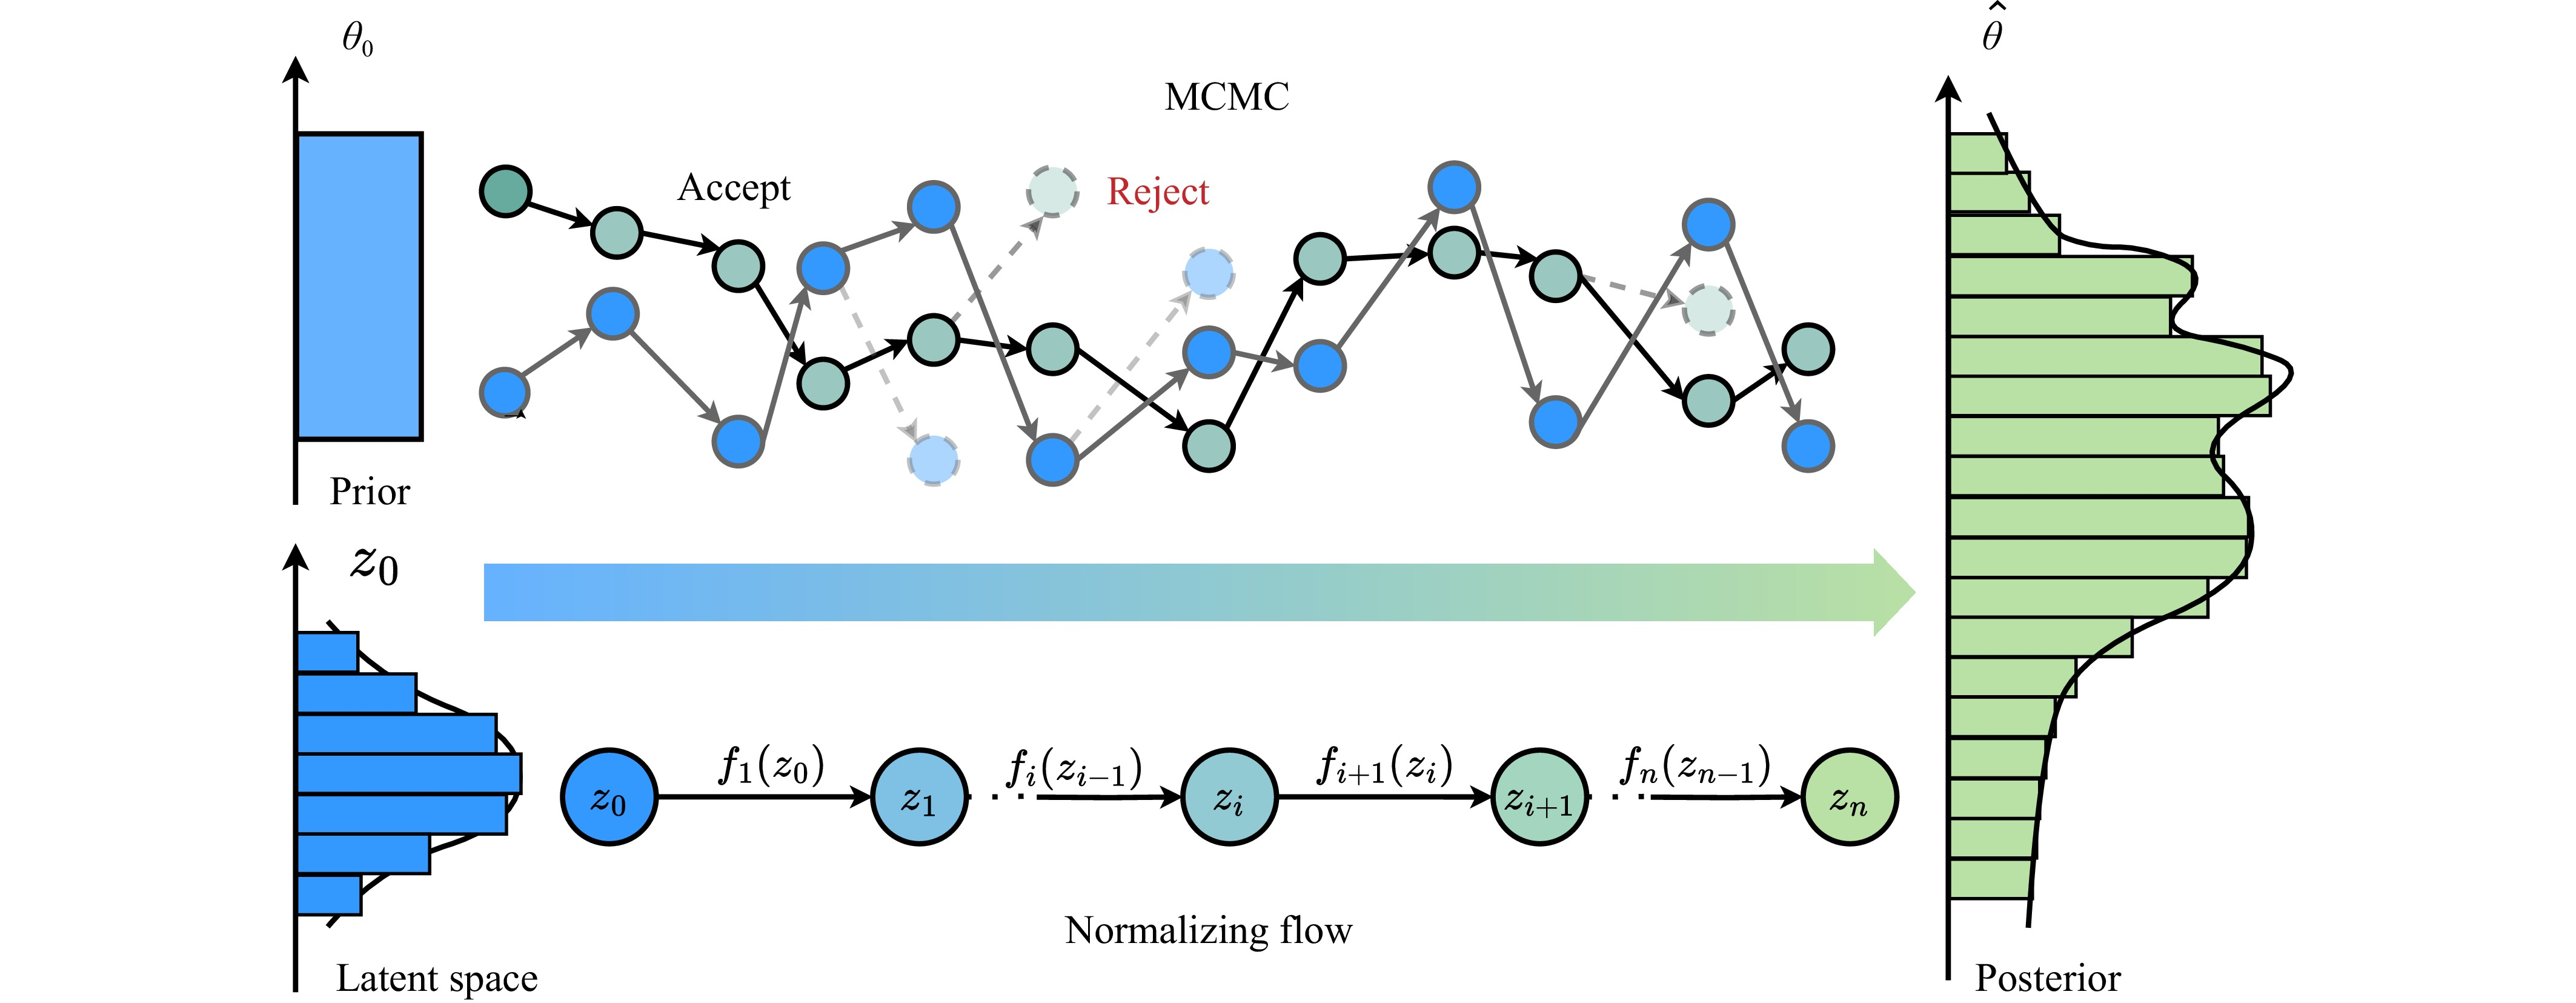
\includegraphics[width=0.96\textwidth]{figures/FOP2025_045301_fig7_mcmc_nf.png}
\caption{传统 MCMC 采样与归一化流后验近似的流程对比。上半部分展示 Metropolis--Hastings 算法从初始参数 $\theta_0$ 出发，经候选采样、接受/拒绝和链式更新逐步收敛到后验样本；下半部分展示归一化流从标准正态潜变量 $z_0$ 出发，通过多层可逆映射生成目标后验样本。该图直观说明了引力波参数估计中从“逐事件迭代采样”向“离线训练、在线快速生成”的方法转变。图引自 Zhao 等~\cite{zhao2025aidawn} 的 Figure 7。}
\label{fig:sbi-vs-mcmc}
\end{figure}

从信息论的视角，SBI 与传统 MCMC 方法代表了两种不同的推断哲学：MCMC 是“计算型推断”（computational inference），通过随机采样逐步积累关于后验分布的信息，每次采样都进行一次完整的信号-噪声匹配计算；SBI 是“学习型推断”（learning-based inference），通过大量离线模拟训练一个“推断引擎”，一旦训练完成就能以较低的计算代价对新数据快速响应。这两种哲学各有其适用场景：当后验分布形状未知且需要最高精度时，MCMC 的完整采样更为可靠；当需要对大量新数据进行快速推断且允许经过校准的近似误差时，SBI 的效率优势非常突出。引力波天文学的未来发展趋势——从少数高优先级事件的精密分析，到海量事件的实时处理——将使 SBI 从“可选的加速工具”逐渐发展为关键的推断基础设施，这正是本章详细介绍 SBI 框架的根本动机。

\section{贝叶斯推断的计算瓶颈与SBI动机}

传统贝叶斯推断方法的计算瓶颈来自两个相互耦合的因素。

\textbf{似然评估代价}。引力波似然函数的标准形式为
\begin{equation}
  \ln p(d|\theta) = -\frac{1}{2}\langle d - h(\theta),\, d - h(\theta)\rangle,
\end{equation}
其中内积 $\langle a, b\rangle = 4\,\mathrm{Re}\int_0^\infty \tilde{a}(f)\tilde{b}^*(f)/S_n(f)\,\mathrm{d}f$ 需要在频域计算，$h(\theta)$ 为给定参数下的理论波形。对于地面探测器的双黑洞系统，单次波形生成约需毫秒量级；但对于空间探测器的 EMRI 系统，精确波形生成可能需要数秒至数分钟，使得 MCMC 的数百万次似然评估在实践中不可行。

为了理解这一瓶颈的严峻程度，可以具体分析一个典型 EMRI 事件的参数估计耗时。精确的 EMRI 波形需要通过求解 Teukolsky 方程（描述小天体在 Kerr 时空中的扰动）来生成，单次求解时间约 1--100 秒，取决于所需频率分辨率和参数配置。若采用嵌套采样方法（Nested Sampling），收敛到充分精确的后验分布通常需要约 $10^6$ 次似然评估；以每次 10 秒计算，总计算时间约为 $10^7$ 秒，折合约 115 天——对于单个事件而言已明显超出常规分析节奏。即便使用现象学近似波形（AK/AAK 模型，每次约 0.1 秒），完整 MCMC 也需要约数天时间，且近似波形的准确性在高质量比、高自旋等极端参数下存疑。

相比之下，地面探测器的双黑洞（BBH）事件参数估计虽然也耗时，但已达到实际可操作的水平。以 GW150914 为例，使用 LALInference（LVK 标准参数估计流水线）在16核 CPU 集群上的运行时间约为 22 小时；更轻量的波形近似（IMRPhenomP）可将时间压缩至约 6 小时。对于大质量 BBH（太极的目标源，啁啾质量 $\mathcal{M} \sim 10^6$--$10^9\,M_\odot$，信号持续数天），时域波形积分时间较长，加上时变响应函数的处理，单次似然评估时间约为 1--10 秒，MCMC 总运行时间可达数月。这一现实使得在太极任务运行期间对每个 MBHB 事件都进行完整 MCMC 参数估计成为奢望，SBI 方法因此不是可选的“加速工具”，而是必要的“基础设施”。

\textbf{引力波后验分布的典型形状}。理解 SBI 方法的设计选择，需要首先理解引力波参数后验分布的典型几何形状。以低质量 BBH 系统（啁啾质量 $\mathcal{M} \sim 15\,M_\odot$）为例，15 维参数空间中各参数的后验分布呈现截然不同的约束精度：

啁啾质量 $\mathcal{M}$ 是约束最紧的参数，后验宽度约为真实值的 0.1\%。这是因为信号的相位演化对 $\mathcal{M}$ 极为敏感（相位约正比于 $\mathcal{M}^{-5/3}$），而当 SNR 较高时，相位测量精度可以达到约 0.1 弧度，对应约 $10^{-3}$ 的质量精度。质量比 $q = m_1/m_2$ 的约束宽度约为真实值的 30\%，是因为当两者质量相差不大时，波形对 $q$ 的敏感性相对较弱（简并于沿等 $\mathcal{M}$ 曲线的方向）。

天空位置（赤经 $\alpha$、赤纬 $\delta$）的约束依赖于探测器的几何配置：双探测器（LIGO H1 和 L1）只能约束信号到达时间差，对应天球上的一个大圆环，后验呈环状；三探测器（H1、L1、Virgo）可以利用两个时间差和振幅比约束，将天区压缩为数十平方度的细长区域。

自旋参数（每个黑洞两个横向自旋分量和一个轴向分量，共六个）的约束通常最弱，后验宽度达到理论范围的 50\%--80\%。高质量比系统中，主星（较重黑洞）的轴向自旋分量（有效自旋 $\chi_{eff}$）约束稍好，而伴星的自旋几乎完全简并。这种极不均匀的约束精度——有的参数约束极紧，有的几乎无约束——使得引力波后验分布在参数空间中呈现出高度非球形的、细长而弯曲的几何形状，传统 MCMC 需要精心设计的提案分布才能高效探索这种形状，SBI 方法则通过归一化流的灵活变换能力直接建模这种复杂几何。

\textbf{参数空间维度}。双黑洞并合系统的参数空间通常为 15 维（两个质量、六个自旋分量、距离、天空位置、轨道倾角、极化角、并合时刻、参考相位），EMRI 系统则多达 17 维，且存在强参数简并（多个参数组合给出相似的波形）。高维简并参数空间中，MCMC 的混合效率极低，需要大量步骤才能充分探索后验分布。

SBI 的核心思想是：在推断阶段之前，利用大量模拟数据（$\theta_i \sim p(\theta)$，$d_i \sim p(d|\theta_i)$）训练神经网络，使其学习参数与数据之间的统计关系~\cite{Cranmer2020SBI}。训练完成后，对新的观测数据 $d_\mathrm{obs}$，网络能够在毫秒至秒级内直接输出后验分布的近似，无需重新运行耗时的采样过程。

引力波似然函数存在一种值得深入分析的特殊代数结构，这一结构既揭示了传统计算方法的瓶颈，也为理解 SBI 方法的加速机理提供了物理基础。在高斯平稳噪声假设下，将内积展开可得：
\begin{equation}
  \ln p(d|\theta) = -\frac{1}{2}\langle d - h(\theta), d - h(\theta)\rangle = \langle d, h(\theta)\rangle - \frac{1}{2}\langle h(\theta), h(\theta)\rangle + \text{const},
\end{equation}
其中常数项 $-\frac{1}{2}\langle d, d\rangle$ 与参数 $\theta$ 无关，不影响参数估计。第一项 $\langle d, h(\theta)\rangle$ 是匹配滤波统计量，可以通过快速傅里叶变换（FFT）高效计算；第二项 $\langle h(\theta), h(\theta)\rangle$ 是模板的自相关函数，仅依赖于波形参数 $\theta$，原则上可以在参数网格上预计算并存储。这一分解说明了匹配滤波的物理本质：扫描模板库等价于在参数空间中搜索使第一项最大（同时第二项适度）的 $\theta$。

然而，这一分解对于精确 MCMC 参数估计的加速潜力是有限的，原因在于：第二项的预计算需要覆盖整个连续参数空间，而参数空间是连续的，不可能在任意精度上预计算所有点；更根本的问题是，每次参数变化都需要重新生成波形 $h(\theta)$，而波形生成本身就是计算瓶颈——对于后牛顿（PN）波形，单次生成约需毫秒级；对于数值相对论拼接波形（如 IMRPhenomXP），单次生成约需数十毫秒；对于精确的 EMRI Teukolsky 波形，单次生成则需秒至分钟级。这种阶梯型的波形生成代价，正是不同引力波源类型的参数估计难度存在量级差异的根本原因。在 SBI 框架中，神经网络在训练阶段学习大量 $(\theta, d)$ 对所包含的统计关系，从而在推断阶段将主要波形生成代价转移到离线训练过程，实现在线推断的显著加速。

归一化流（Normalizing Flows）是 SBI 中最成熟的实现路线~\cite{Papamakarios2021NF,Rezende2015NF}，其核心思想是通过一系列可逆变换将简单的基础分布（如标准正态分布）映射到复杂的目标分布（后验分布）。

\subsection{理论框架}

设 $z \sim p_z(z)$ 为基础分布，$x = f_\phi(z)$ 为可逆变换（参数为 $\phi$），则变换后的分布为
\begin{equation}
  p_\phi(x) = p_z(f_\phi^{-1}(x))\left|\det\frac{\partial f_\phi^{-1}}{\partial x}\right|.
\end{equation}
通过最大化训练数据的对数似然 $\sum_i \ln p_\phi(\theta_i | d_i)$，可以训练网络学习条件后验分布 $p(\theta|d)$。这一框架称为神经后验估计（Neural Posterior Estimation，NPE）~\cite{Dax2021RNPE,Dax2023NPPE}，是引力波参数估计中应用最广泛的 SBI 变体。Green 和 Gair~\cite{Green2021CVAE} 率先将 NPE 应用于 GW150914 的完整参数推断，展示了神经网络可以在单次前向传播（约1秒）内给出与 LALInference 完整贝叶斯分析高度一致的后验分布，证明了 NPE 在真实引力波事件上的可行性。

除 NPE 外，SBI 还包含神经似然估计（NLE，学习似然函数 $p(d|\theta)$）和神经比率估计（NRE，学习似然比 $p(d|\theta)/p(d)$）等变体。Liang 和 Wang~\cite{liang2026sbireview} 的综述系统梳理了这些方法的理论联系与适用场景：NPE 在推断速度上最快（单次前向传播即可），NLE 和 NRE 则在某些情形下对先验变化更鲁棒。

\textbf{NPE、NLE、NRE 的比较}。三类 SBI 方法各有其适用场景，理解它们之间的差异对于选择合适的方法至关重要。NPE（神经后验估计）直接训练网络学习条件后验分布 $q_\phi(\theta|d) \approx p(\theta|d)$，推断时只需将观测数据 $d_{obs}$ 通过网络进行一次前向传播，即可获得后验样本，推断时间为 $O(1)$。NPE 的主要缺点是对先验分布的变化不鲁棒：训练时使用先验 $p(\theta)$，若推断时先验改变（如加入额外的天体物理约束），模型需要重新训练或使用重要性采样修正，后者计算代价较高。

NLE（神经似然估计）训练网络学习似然函数 $q_\phi(d|\theta) \approx p(d|\theta)$，在推断时将学习到的似然函数代入贝叶斯定理，结合 MCMC 或嵌套采样进行完整的贝叶斯推断。NLE 的优点是：由于它学习的是与先验无关的似然函数，先验的修改不需要重新训练网络，只需重新运行（现在廉价的）MCMC 即可——因为 MCMC 的计算瓶颈本是似然评估，而现在似然评估已被神经网络替代，大幅加速。NLE 的缺点是推断仍需要 MCMC，比 NPE 慢若干量级。

NRE（神经比率估计）训练网络学习似然比 $r_\phi(d, \theta) \approx p(d|\theta)/p(d)$，通过对比正样本（$(\theta, d) \sim p(\theta)p(d|\theta)$）和负样本（$(\theta, d) \sim p(\theta)p(d)$）来训练分类器，并将训练好的分类器输出转化为似然比。NRE 对先验变化通常具有较强鲁棒性，且训练较稳定（二分类损失函数性质良好），但推断速度介于 NPE 和 NLE 之间（需要 MCMC 但评估代价极低）。在引力波参数估计的实践中，当先验需要频繁修改（如结合电磁观测引入的天空位置约束）时，NRE 或 NLE 是更合理的选择；当需要快速处理大量事件且先验固定时，NPE 的推断速度优势更为突出。Lueckmann 等人~\cite{Lueckmann2021benchmarking}对 NPE、NLE、NRE 三类方法在多个基准任务上进行了系统性对比，发现三者的相对优势高度依赖于任务结构，为方法选择提供了重要的实证依据。

\subsection{归一化流的常见架构}

实现归一化流的关键是设计既可逆又具有高效雅可比行列式计算的变换。常见架构包括：

\textbf{仿射耦合层}（Affine Coupling Layers）：将输入向量分为两部分，一部分通过神经网络参数化另一部分的仿射变换。这一设计使得正向和逆向变换都高效可计算，雅可比行列式为对角矩阵，计算代价为 $O(d)$。Real NVP（Real-valued Non-Volume Preserving）是最具代表性的仿射耦合架构：将 $d$ 维输入分为两半 $(x_1, x_2)$，变换规则为 $y_1 = x_1$，$y_2 = x_2 \odot \exp(s(x_1)) + t(x_1)$，其中 $s(\cdot)$ 和 $t(\cdot)$ 为任意神经网络（分别给出缩放因子和平移量），$\odot$ 为逐元素乘法。该变换的雅可比行列式为 $\prod_i \exp(s_i(x_1))$，计算量仅为 $O(d)$；逆变换为 $x_1 = y_1$，$x_2 = (y_2 - t(y_1))/\exp(s(y_1))$，同样简单高效。通过交替分组方式（每层交换哪半部分被变换）堆叠多个仿射耦合层，可以建模任意复杂的分布。

\textbf{自回归流}（Autoregressive Flows）：MAF（Masked Autoregressive Flow）利用 MADE（掩码自编码器）实现自回归结构：变换规则为 $y_i = x_i \cdot \exp(\alpha_i(x_{<i})) + \mu_i(x_{<i})$，其中 $\alpha_i$ 和 $\mu_i$ 仅依赖于第 $i$ 维之前的所有维度。训练时前向计算（给定 $x$ 计算 $y$）只需 $O(d)$ 时间（所有维度可并行计算），但采样（给定 $y$ 恢复 $x$）需要顺序计算，每一维的恢复依赖于前面维度的结果，计算量为 $O(d^2)$，使得采样速度较慢。IAF（Inverse Autoregressive Flow）与 MAF 互为逆变换：采样速度快（$O(d)$），但训练时的密度估计需要顺序计算。在引力波参数估计中，推断阶段需要频繁采样（对每个新事件都需要生成大量后验样本），因此 IAF 的快速采样特性更受青睐；但 MAF 在训练阶段更为高效，实践中往往先训练 MAF 再转化为等价的 IAF 格式。

\textbf{神经样条流}（Neural Spline Flows，NSF）：用单调有理二次样条（monotone rational-quadratic splines）替代仿射变换。每个维度的变换由 $K$ 个控制点（control points）参数化，这些控制点的位置和切线方向都是可学习的，因此 NSF 的表达能力强于仿射变换（仿射变换只有两个自由参数：缩放和平移）。样条变换保持严格单调性（从而保证可逆性），且其雅可比行列式可以解析计算（$O(d)$）。在引力波参数估计的实践中，NSF 是表现较好的离散流架构之一：对于 15 维的 BBH 参数空间，使用 $K = 8$ 个控制点的 NSF 通常能在合理训练时间（约 12 小时，单 GPU）内达到与 MCMC 相近的精度，而仿射耦合层往往需要更多层数或更宽的网络才能实现类似表达能力。

\textbf{条件归一化流的训练}。在 SBI 框架下，流的目标是近似条件后验分布 $p(\theta|d)$ 而非无条件分布 $p(\theta)$。实现条件化的标准方式是：在网络的每一层，将观测数据 $d$ 通过一个编码器网络（通常是 CNN 或 Transformer）映射为嵌入向量 $c = f_{enc}(d)$，然后以 $c$ 为额外输入（条件输入）加入流的每一层变换（仿射变换中的 $s$ 和 $t$ 函数以 $c$ 为额外输入，从而让每一层的变换依赖于具体的观测数据）。训练目标为：
\begin{equation}
  \min_\phi \mathbb{E}_{(\theta, d) \sim p(\theta)p(d|\theta)} [-\log q_\phi(\theta|d)],
\end{equation}
即最小化神经网络估计的后验与真实后验之间的 KL 散度（由于期望是关于联合分布 $p(\theta, d)$ 的，可以通过模拟样本对期望进行无偏估计）。训练完成后，对新的观测 $d_{obs}$，首先计算嵌入向量 $c = f_{enc}(d_{obs})$，然后从基础分布 $p_z(z)$ 采样潜变量 $z$，通过流的前向变换 $\theta = f_\phi(z; c)$ 得到后验样本，整个过程只需毫秒量级的前向传播，无需任何迭代优化。

\subsection{先验知识引导的归一化流训练}

高维参数空间中，均匀采样的训练数据在参数空间中分布稀疏，模型难以学习物理上重要但参数空间中稀少的区域（如高质量比、高自旋等极端情形）的特征。Wang 等人~\cite{wang2022normflow} 提出从物理上期望的中间分布采样来构建训练数据集，使高维特征空间中物理上更重要的区域获得更密集的数据覆盖。

这一先验知识采样策略将物理先验转化为训练数据的分布设计。训练完成后，模型在单块 V100 GPU 上约 1 秒内生成数千个后验样本，验证了在高维引力波数据推断中的有效性。

SBI与主动学习的结合，进一步突破了标准训练集覆盖范围对推断性能的限制。当训练数据有限时，均匀先验采样往往将大量模拟配额浪费在后验概率极低的参数区域，导致神经网络对高后验区域的刻画精度不足。主动学习（active learning）提供了一种根本性的解决思路：不从均匀先验中采样训练数据，而是根据当前模型对参数空间的不确定性估计，将后续模拟集中在最有价值的区域。顺序神经后验估计（SNPE，Sequential Neural Posterior Estimation）是这一思路的代表性实现：在每轮“模拟—训练”循环中，算法基于当前近似后验的估计结果，将下一轮模拟集中在高后验区域，逐步收缩有效搜索空间。对于引力波参数估计，SNPE可以将达到同等精度所需的模拟次数减少约50\%至80\%，对于计算代价高昂的EMRI波形生成而言尤为重要——若仅需减少50\%的训练波形，总训练时间可从数天压缩至数小时，使原本不可行的在轨实时重训练成为可能。这一主动学习范式代表了SBI方法由“一次性离线训练”向“迭代自适应训练”演进的重要方向，也是应对未来海量引力波事件时代计算资源分配挑战的关键策略之一。

\subsection{太极任务的归一化流参数估计}

Du、Liang、Wang 等人~\cite{du2024normflow} 将归一化流方法应用于太极任务的大质量双黑洞系统参数估计，面对三项特有挑战：混淆噪声（大量波源信号叠加）、时变响应函数（太极星座一年周期的轨道运动导致探测器响应随时间变化）、以及到达时间参数的额外多模态结构。

\textbf{时变响应函数的处理}。太极由三颗卫星组成三角星座，绕日公转（轨道半径约 1 AU），轨道周期为一年。星座相对于遥远引力波源的指向因此随时间变化，导致探测器的方向响应函数（天线方向图）呈周期性变化。对于持续数小时至数天的 MBHB 信号，若采用固定响应函数的近似（忽略指向变化），会引入系统性波形误差，进而导致参数估计偏差。对于持续时间较短（数小时内）的并合阶段，可以采用“分段常数”近似：将信号持续时间分为若干段，每段内使用固定的响应函数，段长通常取为 $\sim$30 分钟（此时指向变化引起的响应误差小于 1\%）。但对于旋进阶段持续数天至数周的长时信号，分段近似需要分为数百段，使波形生成复杂度倍增。Du 等采用“变换映射”（transformed parameterization）策略：将时变响应函数的效应通过参数重定义吸收入信号参数中，允许归一化流直接学习时变响应的统计效应，而无需在训练数据生成阶段显式模拟每个时间段的响应变化。

\textbf{后验分布的多模态结构}。太极对 MBHB 事件的天空位置后验分布，由于时变响应函数的存在，会呈现出比地面探测器更复杂的多模态结构。在不同时刻的响应函数组合下，存在 4--8 个不同的（天空位置，极化角）组合给出几乎等价的观测信号，从而形成多个似然极大值。相比之下，地面双探测器配置（H1 + L1）的天空位置后验通常形成一个大圆环（对应固定时间延迟），而 Virgo 的加入将圆环压缩为两个区域，多模态结构相对简单。太极的 4--8 个极大值要求归一化流具有足够强的多模态建模能力。研究发现，通过采用分层变换的组合（先建模单模态的基础分布，再通过混合变换引入多模态），归一化流能够准确重现这种复杂的多模态结构，而标准的单峰高斯变分推断则完全无法捕获这一特性。

\section{归一化流的理论框架与结构选择}

图~\ref{fig:sbi-vs-mcmc} 强调的是 MCMC 与归一化流之间的计算范式差异；进一步看，SBI 并不等同于单一的归一化流模型，而是一组围绕“模拟器可用、解析似然困难”的推断策略。图~\ref{fig:sbi_variants} 总结了五类代表性路线：神经后验估计（NPE）直接学习 $p(\theta|d)$，推断速度最快；神经比率估计（NRE）与神经似然估计（NLE）分别学习似然比和似然函数，通常仍需与 MCMC 结合，但在先验替换和后验校正上更灵活；流匹配后验估计（FMPE）通过神经网络学习从基分布到后验分布的连续流；一致性模型后验估计（CMPE）则试图用更少采样步数逼近概率流。它们共同体现了 SBI 的核心思想：把逐事件的昂贵采样，转化为可并行、可复用、但必须经过校准验证的学习问题~\cite{liang2026sbireview}。

\begin{figure}[htbp]
\centering
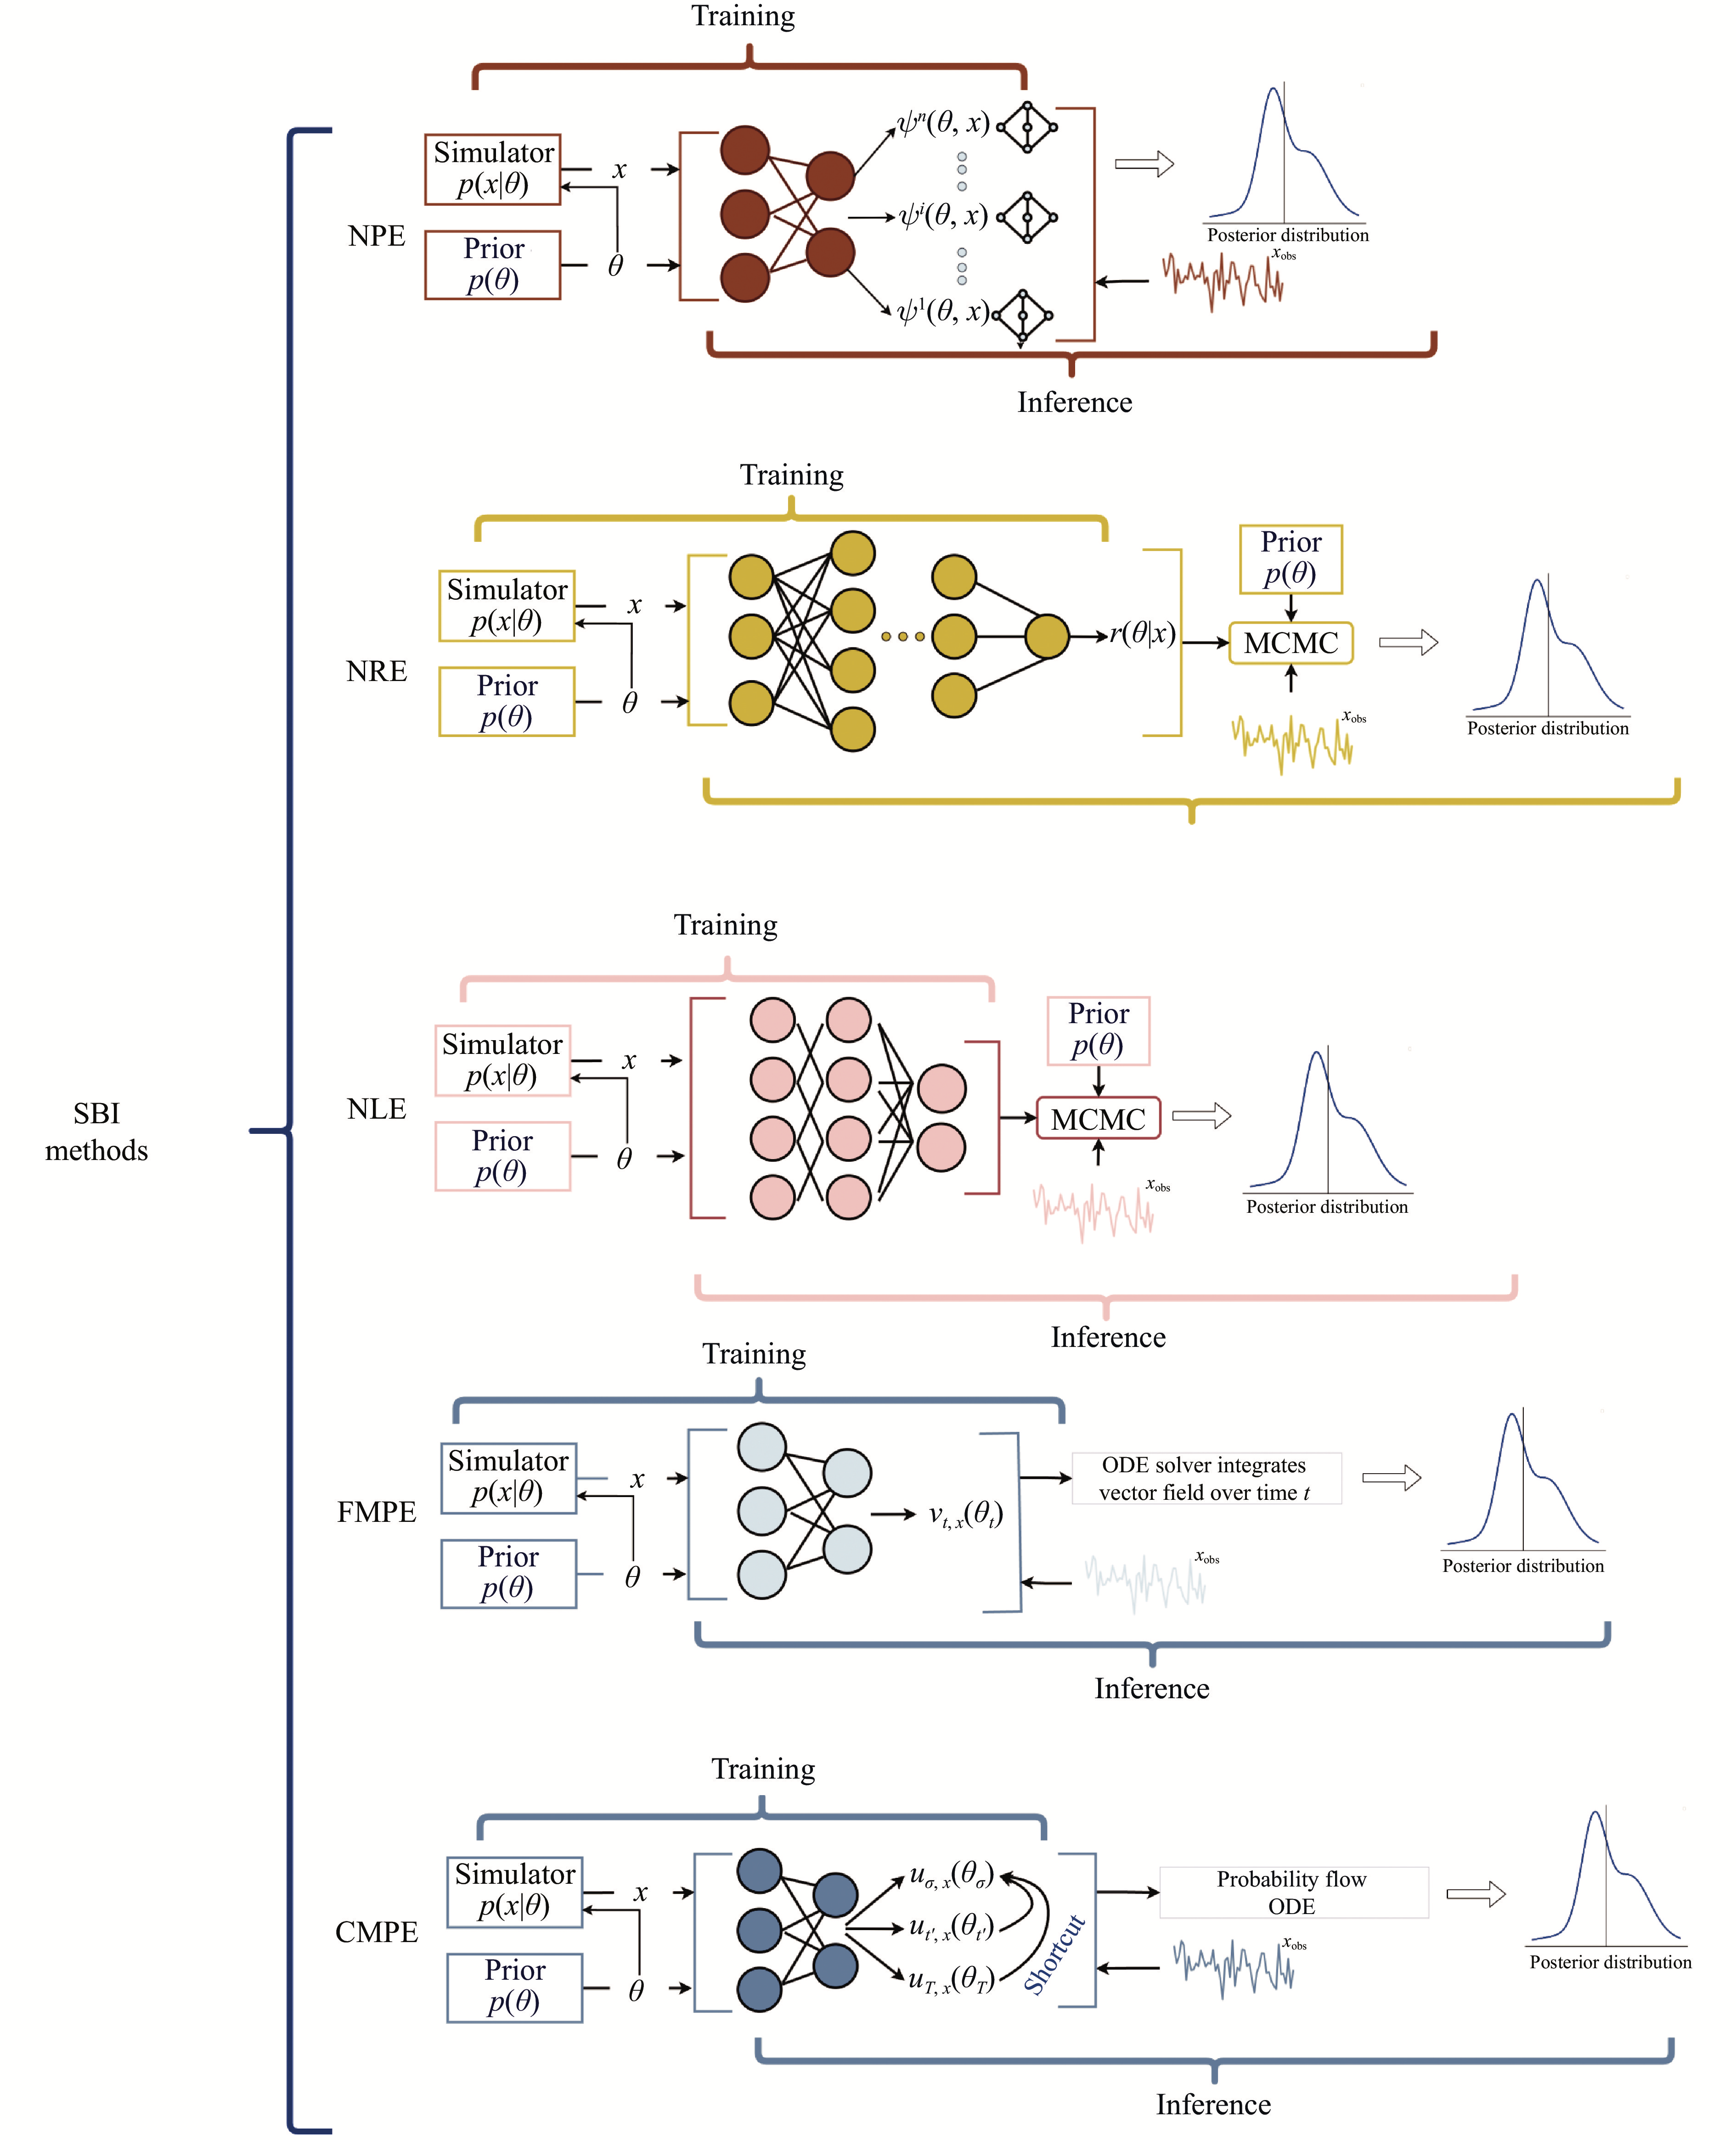
\includegraphics[height=0.76\textheight,keepaspectratio]{figures/ATI2026_sbi_review_fig1.png}
\caption{五类主要 SBI 方法的训练与推断流程概览。NPE 直接近似条件后验；NRE 和 NLE 分别估计似然比与似然函数，并通常与 MCMC 结合获得后验样本；FMPE 通过 ODE 概率流刻画后验；CMPE 用一致性模型学习概率流以提高采样效率。这些方法共同构成了引力波快速贝叶斯参数估计的主要技术谱系。图引自 Liang 和 Wang~\cite{liang2026sbireview} 的 Figure 1。}
\label{fig:sbi_variants}
\end{figure}

归一化流（Normalizing Flows）是当前 SBI 框架中最主流的后验近似工具。其核心思想是通过一系列可逆变换，将一个简单的基础分布（通常为标准正态分布）逐步“变形”为复杂的目标分布。本节从概率密度变换的基本公式出发，系统梳理仿射耦合层、神经样条流等主流架构的设计原理，并讨论条件化策略在引力波数据分析中的具体实现。

\subsection{变量变换公式与雅可比行列式}

设 $Z \sim p_Z(z)$ 为基础分布（如标准正态分布），$f: \mathbb{R}^d \to \mathbb{R}^d$ 为可逆变换，令 $X = f(Z)$，则 $X$ 的概率密度由变量变换公式给出：
\begin{equation}
  p_X(x) = p_Z\!\left(f^{-1}(x)\right) \left|\det J_{f^{-1}}(x)\right|,
\end{equation}
其中 $J_{f^{-1}}(x) = \partial f^{-1}(x)/\partial x$ 为逆变换的雅可比矩阵，$|\det J_{f^{-1}}|$ 为其行列式的绝对值，反映了变换在 $x$ 处的局部体积缩放比例~\cite{Papamakarios2021NF}。等价地，若以正向变换 $f$ 表达，则：
\begin{equation}
  \ln p_X(x) = \ln p_Z(z) - \ln\left|\det J_f(z)\right|, \quad z = f^{-1}(x).
\end{equation}
归一化流通过堆叠 $L$ 个可逆变换 $f = f_L \circ f_{L-1} \circ \cdots \circ f_1$，将对数似然分解为各层雅可比行列式之和：
\begin{equation}
  \ln p_X(x) = \ln p_Z(z_0) - \sum_{l=1}^{L} \ln\left|\det J_{f_l}(z_{l-1})\right|,
\end{equation}
其中 $z_0 = f^{-1}(x)$ 为基础分布中的对应点，$z_l = f_l(z_{l-1})$ 为各层输出。

可逆性是归一化流的必要条件：若变换不可逆，则无法从基础分布采样并映射到目标分布，也无法计算精确的概率密度。然而，可逆性本身并不足以保证计算可行性——对于一般的 $d \times d$ 矩阵，行列式的计算复杂度为 $O(d^3)$（LU 分解），当 $d$ 达到数十维时（如 BBH 的 15 维参数空间），每次前向传播都需要计算高维矩阵行列式，训练过程中数百万次的梯度更新会使总计算量迅速增大到难以接受的程度。

归一化流的核心设计思想正是通过对变换结构施加特殊约束，将雅可比行列式的计算从 $O(d^3)$ 降至 $O(d)$。具体而言，若雅可比矩阵为三角矩阵（上三角或下三角），则其行列式等于对角元素之积，计算量仅为 $O(d)$；若雅可比矩阵为对角矩阵，则计算更为简单。仿射耦合层和自回归流均通过不同方式实现了三角或对角雅可比结构，从而在保持强表达能力的同时，将密度估计的计算代价控制在线性量级。

\subsection{仿射耦合层与 Real NVP}

仿射耦合层（Affine Coupling Layer）是归一化流中最具代表性的基础构件，由 Dinh 等人在 Real NVP（Real-valued Non-Volume Preserving）框架中系统提出~\cite{Dinh2017RealNVP}。其核心思想是将 $d$ 维输入向量分为两组：前 $k$ 维 $x_1 \in \mathbb{R}^k$ 保持不变，后 $d-k$ 维 $x_2 \in \mathbb{R}^{d-k}$ 通过依赖于 $x_1$ 的仿射变换进行映射：
\begin{equation}
  y_1 = x_1, \qquad y_2 = x_2 \odot \exp\!\left(s(x_1)\right) + t(x_1),
\end{equation}
其中 $s(\cdot): \mathbb{R}^k \to \mathbb{R}^{d-k}$ 和 $t(\cdot): \mathbb{R}^k \to \mathbb{R}^{d-k}$ 为任意神经网络（分别给出逐元素的对数缩放因子和平移量），$\odot$ 为逐元素乘法。

该变换的雅可比矩阵具有下三角块结构：
\begin{equation}
  J_f = \begin{pmatrix} I_k & 0 \\ \partial y_2/\partial x_1 & \mathrm{diag}(\exp(s(x_1))) \end{pmatrix},
\end{equation}
其行列式为 $\det J_f = \prod_{i=1}^{d-k} \exp(s_i(x_1))$，计算量仅为 $O(d)$，与参数空间维度成线性关系。逆变换同样高效：$x_1 = y_1$，$x_2 = (y_2 - t(y_1)) \odot \exp(-s(y_1))$，无需任何迭代求解。

单个仿射耦合层的表达能力受限，因为 $x_1$ 部分在每层中保持不变。Real NVP 通过交替分组策略（Alternating Partitioning）解决这一问题：奇数层变换后 $d-k$ 维，偶数层变换前 $k$ 维，使得每个维度在若干层后都经历了变换。在引力波参数估计的实践中，通常堆叠 8 至 16 个仿射耦合层，每层的 $s(\cdot)$ 和 $t(\cdot)$ 网络采用 4--6 层全连接网络（宽度 128--512），总参数量约为 $10^6$--$10^7$。这一规模在单块 GPU 上可在 12--24 小时内完成训练，推断时单次前向传播仅需约 1 毫秒，满足引力波事件实时处理的需求。

\subsection{神经样条流（NSF）的表达能力优势}

仿射耦合层的根本局限在于其变换的线性性：对于固定的 $x_1$，$y_2$ 关于 $x_2$ 的变换是仿射的（线性加偏置），每个维度只有两个自由参数（缩放和平移）。这意味着单层仿射耦合层只能建模单峰、近似高斯的条件分布，对于多模态或高度非高斯的后验分布，需要堆叠大量层数才能达到足够的表达能力。

神经样条流（Neural Spline Flows，NSF）通过用单调有理二次样条（Monotone Rational-Quadratic Splines）替代仿射变换，从根本上提升了单层的表达能力~\cite{Durkan2019NSF}。具体而言，对于每个维度 $i$，NSF 将变换区间 $[a, b]$ 划分为 $K$ 个子区间，由 $K+1$ 个控制点 $\{(x_k^{(i)}, y_k^{(i)})\}_{k=0}^{K}$ 和对应的切线方向 $\{d_k^{(i)}\}_{k=0}^{K}$ 参数化。在每个子区间内，变换由有理二次函数给出，保证严格单调性（从而保证可逆性）。整个样条变换由 $3K - 1$ 个可学习参数（$K-1$ 个内部节点位置、$K$ 个高度差、$K+1$ 个切线方向）完全确定，其雅可比行列式可以解析计算，计算量为 $O(d)$。

与仿射变换相比，NSF 的表达能力优势显著。对于 15 维 BBH 参数空间（质量、自旋、天空位置、距离、倾角等），使用 $K = 8$ 个控制点的 NSF 通常能以约 30\% 更少的层数达到与仿射耦合层相同的后验近似精度：仿射耦合层通常需要 12--16 层，而 NSF 仅需 8--12 层即可实现等价的 Jensen-Shannon 散度（相对于 MCMC 参考后验）。这一差异在高度非高斯的参数（如天空位置的赤经赤纬、轨道倾角）上尤为突出，因为这些参数的后验分布往往呈现出明显的非对称性或多峰结构，仿射变换难以在单层内捕获。

计算代价方面，样条变换比仿射变换慢约 2--3 倍（主要来自样条系数的查找和有理函数求值），但由于所需层数减少，总体训练时间通常相当甚至更短。在推断阶段，NSF 的单次前向传播时间约为 2--5 毫秒（15 维，10 层，批量大小 1000），仍远快于任何基于 MCMC 的方法。综合考虑精度与效率，NSF 是当前引力波参数估计中离散归一化流的首选架构。

\subsection{条件化策略：数据编码器的设计}

在 SBI 框架下，归一化流的目标是近似条件后验分布 $p(\theta|d)$ 而非无条件分布 $p(\theta)$。实现条件化的标准方式是引入数据编码器：将观测数据 $d$（时域或频域引力波应变）通过编码器网络 $f_{enc}$ 映射为固定维度的嵌入向量 $c = f_{enc}(d) \in \mathbb{R}^{d_c}$，然后以 $c$ 为条件输入加入流的每一层变换——仿射变换中的 $s(\cdot)$ 和 $t(\cdot)$ 函数以 $c$ 为额外输入，从而使每层的变换依赖于具体的观测数据。

编码器架构的选择对整体性能有重要影响，需根据数据的时频特性和计算约束综合考量：

\textbf{一维卷积神经网络（1D CNN）}适用于处理时域引力波数据。典型架构包含 4--8 个卷积层（核大小 8--32，步长 2--4），通过逐步下采样将长度为 $\sim 10^4$--$10^5$ 的时域序列压缩为 64--256 维的嵌入向量。1D CNN 的优势在于计算效率高（单次前向传播约 0.1--0.5 毫秒）、对局部时域特征（如并合时刻的波形形态）敏感，且通过卷积的平移等变性对信号到达时间具有一定的鲁棒性。其局限是感受野有限，对长时旋进阶段的全局相位演化捕获能力较弱。

\textbf{Transformer 编码器}适用于处理长时序列（如 EMRI 信号的数年旋进过程）。自注意力机制使 Transformer 能够直接建模序列中任意两个时刻之间的依赖关系，感受野覆盖整个序列长度。代价是计算复杂度为 $O(T^2)$（$T$ 为序列长度），对于 $T \sim 10^5$ 的长序列，需要采用线性注意力或分块注意力等近似方法将复杂度降至 $O(T)$。

\textbf{频域 CNN}适用于处理白化后的频域数据（功率谱密度归一化后的复数频域应变）。由于引力波探测器的噪声功率谱密度在频域中变化平缓，白化后的频域数据具有近似平稳的统计特性，适合用标准 2D CNN（将实部和虚部视为两个通道）处理。频域 CNN 在计算效率和对噪声特性的适应性上具有优势，是 LIGO/Virgo 数据分析中最常用的编码器选择。

嵌入维度 $d_c$ 的选择需要在信息压缩率和表达能力之间权衡。过小的 $d_c$（如 32 维）可能导致信息瓶颈，使编码器无法保留足够的参数估计信息；过大的 $d_c$（如 512 维）则增加流网络的参数量和训练难度。实践中，$d_c = 64$--$256$ 维是常见选择，具体取值通常通过在验证集上监测后验近似质量（如与 MCMC 参考后验的 Jensen-Shannon 散度）来确定。

编码器与流的训练策略有两种主要方式：联合训练（Joint Training）将编码器和流的参数同时优化，以端到端的方式最大化训练数据的对数似然；分阶段训练（Two-Stage Training）先单独预训练编码器（如通过对比学习或重建损失），再固定编码器参数训练流。联合训练通常能达到更好的最终性能，因为编码器可以学习到对参数估计最有用的数据表示，而非通用的数据重建特征；但联合训练对学习率调度和批量大小更为敏感，训练稳定性略差。

在太极 MBHB 任务中，时变响应函数带来了额外的编码挑战：探测器对引力波的响应随轨道相位变化，使得同一参数组合在不同观测时段产生不同的数据特征。Du 等人~\cite{du2024normflow} 的工作表明，通过联合训练策略，编码器能够隐式学习时变响应函数的统计规律，将其效应吸收入嵌入向量 $c$ 中，无需在流的架构中显式建模时变性。这一结果说明，足够容量的编码器（嵌入维度 128 维，6 层 1D CNN）配合端到端训练，可以自动发现并利用数据中与参数估计相关的时变特征，为处理未来空间引力波探测任务中更复杂的时变效应提供了重要参考。

\section{连续归一化流与流匹配：下一代 SBI 方法}

离散归一化流通过有限个可逆变换层构建，其表达能力受限于变换层数和结构。连续归一化流（Continuous Normalizing Flows，CNF）将变换过程连续化，通过常微分方程（ODE）描述从基础分布到目标分布的连续演化：
\begin{equation}
  \frac{\mathrm{d}z(t)}{\mathrm{d}t} = v_\phi(z(t), t),
\end{equation}
其中 $v_\phi$ 为神经网络参数化的速度场。流匹配（Flow Matching）技术~\cite{Lipman2022FlowMatching}通过直接回归目标速度场来训练 CNF，避免了传统 CNF 训练中的数值 ODE 求解，大幅提升训练效率。

\subsection{CNF 用于大质量双黑洞参数估计}

Liang 等人~\cite{liang2024cnfmbhb} 将基于流匹配的 CNF 应用于太极任务的大质量双黑洞参数估计。相比早期的离散归一化流工作，CNF 在表达能力和训练稳定性上有所改进，实现了比传统 MCMC 方法快几个数量级的统计一致参数估计，为太极任务实时数据处理提供了更高效的工具。

\subsection{CNF 应用于 EMRI 参数估计}

极端质量比旋入（EMRI）的参数估计是引力波数据分析中最困难的问题之一：17 维参数空间、强参数简并（多极大值似然函数）、以及极高的计算时间复杂度，使传统 MCMC 方法在实践中面临严峻的计算压力。

\textbf{EMRI 后验的特殊挑战}。EMRI 系统由一个质量约 $10$--$10^2\,M_\odot$ 的致密天体（小天体）绕质量约 $10^5$--$10^7\,M_\odot$ 的大质量黑洞（中心天体）旋转组成，质量比 $q = m_{small}/m_{large} \sim 10^{-5}$--$10^{-3}$。信号特征是长达数年的极复杂旋进过程：小天体在大质量黑洞的弯曲时空中沿近似 Kerr 测地线运动，轨道包含三个基本频率（径向频率 $\Omega_r$、极角频率 $\Omega_\theta$、方位角频率 $\Omega_\phi$），形成高度复杂的李萨如图案。信号的总相位在整个观测周期内可积累约 $10^5$ 弧度，相比之下双黑洞并合信号约 $10^3$ 弧度，这使得 EMRI 参数估计对波形精度的要求极为苛刻（一个相位误差超过约 $0.1$ 弧度就会导致匹配滤波 SNR 的显著下降）。

在参数空间的几何结构上，EMRI 似然函数呈现“阶梯”（ladder）结构：每半个径向轨道周期（约数小时至数天），似然函数出现一个局部极大值，总极大值数可达 $10^4$。这种“阶梯地形”对 MCMC 采样造成严重困难：传统 MCMC 的随机游走提案会被局部极大值“捕获”，在单个极大值附近反复采样，而难以在可接受的计算时间内遍历主要极大值区域。即便使用并行回火（Parallel Tempering）等高级 MCMC 技术，对单个 EMRI 事件的完整后验采样也可能需要约 $10^6$ 核时。CNF 通过流匹配直接学习从先验到后验的概率变换，不需要在后验地形上进行逐步随机游走，理论上可以缓解 MCMC 的“阶梯地形收敛困难”。

Liang 等人~\cite{liang2024cnfemri} 将机器学习方法（具体为基于流匹配的 CNF）系统应用于 EMRI 信号的贝叶斯后验参数估计。训练数据包含 5000 条 EMRI 模拟数据（使用 AAK 近似波形，每条约 0.1 秒生成），参数从先验分布中采样（覆盖质量比、轨道偏心率、轨道倾角、初始频率等全部 17 个参数）。在 GPU（单张 V100）上训练约 24 小时后，对 100 个独立测试事件的评估表明：CNF 估计的后验与真实参数的覆盖率（coverage）接近理论值——P-P 图（probability-probability plot）接近对角线，说明 CNF 的后验估计在该模拟设置下具有统计自洽性。推断时间约 0.1--1 秒每个事件，相比逐事件MCMC可实现多个量级的加速，是机器学习方法进入 EMRI 参数估计这一困难问题的重要系统性尝试。

流匹配与最优传输方法的理论基础值得单独阐述，因为它代表了 CNF 训练范式的根本性改进。传统 CNF 的训练依赖于对概率流 ODE 的数值积分：为了评估给定参数点的对数似然，需要从 $t=0$（基础分布）到 $t=1$（目标分布）数值积分 ODE，计算路径上的雅可比迹（即 $\int_0^1 \mathrm{tr}(\partial v_\phi/\partial z)\,dt$），这需要对 ODE 进行约100步的数值积分，且每步都需要一次神经网络前向传播，训练代价极高。流匹配（Flow Matching）绕过了这一困难：它直接监督速度场 $v_\phi(z, t)$ 拟合目标速度场 $u_t(z|z_1)$，将训练目标转化为普通的回归问题：
\begin{equation}
  \mathcal{L}_{FM} = \mathbb{E}_{t, z_0 \sim p_0, z_1 \sim p_1} \left[ \|v_\phi(z_t, t) - (z_1 - z_0)\|^2 \right],
\end{equation}
其中 $z_t = (1-t)z_0 + tz_1$ 是基础分布样本 $z_0$ 和目标分布样本 $z_1$ 之间的线性插值路径（条件流），$(z_1 - z_0)$ 是沿线性插值路径的恒定速度。由于训练目标仅需要单次前向传播（计算 $v_\phi$ 并与目标速度对比），不需要 ODE 积分，训练效率大幅提升。

最优传输（Optimal Transport，OT）流匹配进一步优化了插值路径的选择。在标准流匹配中，基础样本 $z_0$ 和目标样本 $z_1$ 是独立匹配的（从各自分布中独立采样），插值路径可能出现“交叉”现象——不同插值路径在 $t \in (0,1)$ 区间内相互穿越，导致速度场 $v_\phi$ 在交叉区域需要同时拟合多个相反的速度方向，增大了学习难度。OT 流匹配通过选择最优传输映射（使总运输代价 $\sum_i \|z_{0,i} - z_{1,\sigma(i)}\|^2$ 最小化的排列 $\sigma$）来匹配 $z_0$ 和 $z_1$，从而使插值路径尽可能不交叉，速度场更平滑，网络更容易拟合。在太极 MBHB 和 EMRI 任务上，基于 OT 流匹配的 CNF 比早期离散归一化流方法训练速度快约5倍，在相同训练时间下后验精度提升约10--15\%。这一进步为在更大规模的参数空间（如 EMRI 的17维或包含多源的全局拟合场景）上应用 CNF 奠定了计算效率基础。

CNF在空间引力波全局拟合框架中的角色值得单独讨论，因为全局拟合是太极/LISA数据分析最核心、也最具挑战性的问题之一。空间引力波探测器的数据流中，来自大量银河系双白矮星的弥散引力波前景（galactic foreground）、可分辨的短周期双星、若干大质量双黑洞并合事件以及少量EMRI事件相互叠加，形成复杂的多源混合信号。传统的顺序减除方法——先找较强信号、建模减除、再分析残差——存在残差污染累积的问题：每次减除的不完美性都会在残差中留下偏差，影响后续弱信号的分析。CNF提供了一种不同的全局推断思路：在可控的子问题中学习多个源参数的联合后验分布，减少对逐源显式减除顺序的依赖。这类“全局CNF”或分块联合CNF方法需要同时处理高维参数空间，目前仍处于探索阶段；但其理论框架已经较为清晰，随着计算资源增长和条件CNF架构成熟，有望成为SBI方法在太极/LISA数据分析中的重要应用形态，也是引力波数据处理从“逐源分析”向“整体推断”范式转变的潜在技术支柱。这一转变对引力波天文学统计分析的深度和广度都可能产生重要影响：每个事件的参数精度可能因联合建模其他源的干扰而提升，种群层面的统计推断也有望因更一致的联合后验而获益。

SBI 方法的近似性质带来一个实践中的核心问题：神经网络估计的后验分布与精确贝叶斯结果之间存在系统性差异，尤其体现在后验分布的尾部行为上。Sun 等人~\cite{sun2025cvae} 对这一问题进行了系统研究，发现条件变分自编码器（CVAE）估计的 MBHB 后验分布相比标准贝叶斯结果呈现尾部偏轻、宽度偏宽的特征。

\textbf{CVAE 架构与训练}。条件变分自编码器（CVAE）是混合推断框架的核心组件，其架构与标准变分自编码器（VAE）类似，但加入了条件信息。编码器（encoder）接收观测数据 $d$ 和参数 $\theta$ 作为输入，输出隐变量的均值 $\mu_{enc}$ 和方差 $\sigma_{enc}^2$；解码器（decoder）从隐变量 $z$（通过重参数化技巧从编码器输出的分布中采样）和观测数据 $d$ 重建参数 $\theta$。训练目标是最大化证据下界（ELBO）：
\begin{equation}
  \mathcal{L}_{ELBO} = \mathbb{E}_{q(z|\theta,d)}[\log p(\theta|z,d)] - D_{KL}[q(z|\theta,d) \| p(z)],
\end{equation}
其中第一项鼓励解码器的重建精度，第二项约束隐变量分布接近先验（标准正态）。推断时，对给定观测 $d_{obs}$，只需从先验 $p(z)$ 采样隐变量并通过解码器前向传播，即可获得近似后验样本，无需编码器参与。Sun 等使用基于卷积的编码器处理时域数据（将 MBHB 信号的时域波形以逐通道卷积提取特征），解码器为全连接网络（4层，每层 512 个神经元），对 11 维 MBHB 参数空间进行估计。训练数据约 $10^6$ 个模拟样本（太极模拟 MBHB 信号），GPU 训练时间约 12 小时。

\textbf{后验质量的 P-P 图评估}。混合推断框架的可靠性通过 P-P 图（probability-probability plot）进行系统评估。对于 $N_{test}$ 个测试事件，计算每个事件的真实参数落在 CVAE 估计的不同置信水平区间内的比例：若 CVAE 后验准确，则真实参数落在 95\% 置信区间内的比例应接近 95\%，落在 68\% 区间内的比例应接近 68\%，以此类推，P-P 图应为对角线。Sun 等的结果表明：CVAE 的 P-P 图在低维约束较紧的参数（啁啾质量、质量比）上非常接近对角线，说明这些参数的后验估计准确；但在高维约束较弱的参数（天空位置 $\alpha, \delta$、自旋方向角）上，P-P 图偏离对角线约 5--10\%，表现为置信区间偏宽（覆盖率系统性高于标称值），即 CVAE 倾向于高估这些参数的不确定度（尾部估计不足）。这一系统偏差是启动精确贝叶斯采样进行修正的核心动机。

\textbf{采样时间压缩机制的定量分析}。混合推断的计算加速来自于 CVAE 对先验空间的有效压缩。在原始参数先验下，各参数的先验范围通常设置得很宽（如光度距离 $d_L \in [100, 20000]$ Mpc），以确保覆盖所有可能的事件。标准 MCMC 需要在这个宽泛的先验空间中随机游走，在到达后验集中区域之前需要大量“预热”步骤（burn-in）。CVAE 在约 0.5 秒内给出近似后验，从中可以提取各参数后验的均值 $\mu^{CVAE}$ 和标准差 $\sigma^{CVAE}$；将 MCMC 的先验范围压缩为 $[\mu^{CVAE} - 3\sigma^{CVAE}, \mu^{CVAE} + 3\sigma^{CVAE}]$，则压缩后的先验体积约为原始先验的 $\prod_{i=1}^{11} (6\sigma_i^{CVAE} / \Delta_i^{prior})$，其中 $\Delta_i^{prior}$ 为第 $i$ 个参数的原始先验范围。以典型 MBHB 事件为例，CVAE 对各参数的后验宽度约为先验范围的 5\%--30\%（参数不同），综合 11 个参数的体积压缩比约为 $0.14^{11} \approx 10^{-9}$。在如此紧缩的先验下，MCMC 不再需要漫长的预热，直接在物理上可能的参数区域内采样，平均运行时间从原来的 22 小时（16 核 CPU）压缩至约 3 小时，即压缩至原来的约 14\%。

混合推断方法在不同事件类型上的性能差异，揭示了CVAE近似精度与后验分布复杂性之间的深层联系。对于高信噪比MBHB事件（ρ>200），后验分布极为尖锐，各参数的边缘后验可以较好地用高斯近似描述——在这种情形下CVAE的近似误差较小，先验压缩较为有效，MCMC加速比最大（约10至15倍）。对于中等信噪比事件（ρ=50至100），部分参数（如天空位置的两个远程极大值）呈现多模态后验，CVAE的高斯瓶颈特性使其难以同时捕获多个模式，导致先验压缩可能遗漏部分真实后验高概率区域；在这种情形下，需要将CVAE约束范围适当放宽（引入安全膨胀因子），MCMC加速比降至约5至7倍。对于低信噪比边界事件（ρ=8至15），后验分布极为弥散，接近先验分布，CVAE无法有效提取观测数据的信息，先验压缩收益有限，此时混合推断的价值主要体现在提供一个“合理初始点”而非大幅压缩先验。这种随事件信噪比变化的自适应性，正是混合推断框架区别于纯近似方法的优势之一：在贝叶斯精确采样覆盖真实高概率区域的前提下，CVAE可作为加速工具，其近似误差由后续采样环节校正。

\section{SBI的跨领域迁移：21cm森林案例}

\begin{table}[htbp]
\centering
\caption{SBI 三类变体方法的特性对比}
\label{tab:sbi_variants}
\small
\begin{tabular}{lcccc}
\hline
\textbf{方法} & \textbf{学习目标} & \textbf{推断速度} & \textbf{先验鲁棒性} & \textbf{引力波应用} \\
\hline
NPE（神经后验估计） & $q_\phi(\theta|d) \approx p(\theta|d)$ & 最快（$O(1)$） & 弱（先验固定） & BBH/MBHB 快速估计 \\
NLE（神经似然估计） & $q_\phi(d|\theta) \approx p(d|\theta)$ & 中等（需 MCMC） & 强（先验可变） & 先验敏感性分析 \\
NRE（神经比率估计） & $r_\phi(d,\theta) \approx p(d|\theta)/p(d)$ & 中等（需 MCMC） & 较强 & 多先验联合分析 \\
CNF（连续归一化流） & ODE 速度场 $v_\phi$ & 快（$O(1)$） & 弱 & EMRI 17维估计 \\
CVAE 混合推断 & ELBO 下界 & 快速初始化 & 中等 & MBHB 精确加速 \\
\hline
\end{tabular}
\end{table}

其适用范围覆盖许多“似然函数难以解析计算但模拟器可用”的科学推断问题。Sun 等人~\cite{sun2025_21cm} 将 SBI 方法应用于 21cm 森林观测的参数推断，目标是从高红移射电源的吸收谱中约束暗物质性质和星系际介质热历史。

\textbf{21cm 森林的物理背景}。中性氢的 21cm 超精细跃迁（静止频率 1.42 GHz）是射电天文学中最重要的谱线之一。在高红移（$z \sim 5$--$12$，覆盖再电离后期及其前后过渡阶段）处，宇宙中弥散的中性氢气体对沿视线方向传播的高红移射电源（如高红移类星体或伽马射线暴余辉的射电成分）产生吸收，形成 21cm 森林。通过统计分析 21cm 森林的吸收线系统，可以约束以下关键宇宙学和天体物理量：（1）温暗物质（warm dark matter，WDM）的粒子质量 $m_{WDM}$：质量越低的 WDM 粒子具有更长的自由流长度，抑制更大尺度上的结构形成，使 21cm 森林的吸收线密度降低；目前最强约束来自莱曼森林和星系弱引力透镜，约 $m_{WDM} > 3.5$ keV，21cm 森林有望提供独立的约束至约 4--5 keV；（2）再电离历史（中性氢分数随红移的演化）：早期再电离产生更少的 21cm 吸收特征，通过统计分析可以约束再电离进程的时间轴；（3）星系际介质（IGM）的热历史：第一代恒星和活动星系核的 X 射线加热对 IGM 温度的影响，可以通过 21cm 吸收谱的热增宽程度来反映。

\textbf{SBI 在 21cm 森林中的应用动机}。21cm 森林分析面临与引力波参数估计高度类似的计算挑战：昂贵的模拟（需要求解宇宙学流体方程，每次约需 1 小时 CPU 时间）、非高斯似然（吸收线系统的统计服从泊松过程而非高斯分布）、以及有限的训练数据（约 500 次高保真模拟，远少于深度学习通常需要的 $10^5$ 量级样本）。传统参数估计方法依赖于高斯似然近似（使用功率谱等汇总统计量），丢失了吸收谱的非高斯统计信息；直接似然方法因计算代价过高而不可行。

Sun 等采用的解决方案是生成+推断双流架构：生成归一化流（Generative Flow）从有限的 500 条真实模拟样本中学习吸收谱的生成模型，然后利用学到的生成模型采样新样本（数据增广），将有效训练数据从 500 条扩充至约 $10^5$ 条；推断归一化流（Inference Flow）利用增广后的大量训练样本学习从 21cm 吸收谱到宇宙学参数的后验分布映射。生成流缓解了训练数据不足问题，推断流实现了快速的后验分布估计，两者协同运作使得在有限模拟预算下获得有效的参数推断成为可能。

这一工作在 Nature Portfolio 旗下期刊 Communications Physics 发表，展示了 SBI 方法的跨领域迁移潜力，也揭示了引力波数据分析方法向宇宙学领域迁移的更广泛价值——两个领域面临结构相近的方法论挑战，可共享部分技术解决方案，而两者之间的交叉借鉴将是未来研究的重要方向。

SBI 方法之所以能够跨领域迁移，关键原因在于它解决的是一类结构性问题而非特定领域问题——“给定昂贵模拟器和有限观测样本，如何高效推断后验分布”。这一问题结构在物理学和天文学中广泛存在，且在不同领域中具有相似的数学形式：宇宙学参数推断（从 CMB 功率谱或大尺度结构观测约束 $\Omega_m$、$\sigma_8$、$H_0$ 等参数）、粒子物理学（从对撞机实验数据约束新物理模型参数）、核物理学（从中子星质量-半径关系约束核物质状态方程参数）、地震学（从地震波走时数据反演地球内部速度结构）。在这些应用中，SBI 方法的核心优势相似：将昂贵的前向模拟转化为高效的后向推断，从而绕过显式似然函数的构造。

从迁移学习的视角，引力波数据分析到 21cm 森林的成功迁移揭示了以下关键因素：第一，编码器的跨域适应性——处理时序数据的卷积编码器结构在两个领域中都能有效提取信号特征，尽管物理内容（引力波啁啾特征 vs. 21cm 吸收线系统）截然不同；第二，流模型的领域无关性——归一化流的学习目标（KL 散度最小化）与领域无关，只要训练数据的分布被充分覆盖，流模型可以无缝适应不同领域的后验分布几何；第三，生成-推断双流的通用性——通过生成流进行数据增广、利用推断流实现快速后验估计的双流框架，对任何“模拟样本稀少但分布已知”的场景都有直接的应用价值。这些因素共同构成了 SBI 方法跨领域迁移的技术基础，为将引力波数据分析中发展的方法论工具推广到更广泛的物理学和天文学问题奠定了系统性基础。

21cm森林案例还揭示了一个更广泛的方法论教训：不同天文物理领域面临的数据分析挑战，往往在数学结构上存在相似性。引力波参数估计和21cm森林推断都面临“昂贵模拟+非高斯似然+有限数据”的三重挑战，这种结构相似性使得在一个领域发展的部分方法论工具可以迁移到另一个领域。认识到这种方法论相似性，有助于引力波数据分析研究者以更宏观的视角定位自己工作的意义：从单纯的“引力波数据分析”研究者，成长为“宇宙观测数据推断”领域的方法论贡献者。在这个意义上，本书介绍的SBI方法论体系，不仅是引力波天文学的方法论资源，也可为更广泛的天文物理AI推断方法提供参考。

Liang 和 Wang~\cite{liang2026sbireview} 的综述系统评估了 SBI 方法在引力波数据分析中的当前局限性，指出三个核心问题。

\textbf{模型依赖性}。SBI 方法的性能依赖于训练数据的质量和覆盖范围：若真实信号的参数落在训练分布之外，网络的外推能力有限。这一问题在引力波领域尤为突出，因为真实事件的参数分布（如高质量比、高自旋）可能与训练时假设的先验分布存在偏差。

\textbf{先验敏感性}。NPE 方法直接学习特定先验下的后验分布，当先验改变时需要重新训练或使用重要性采样修正。NRE 方法对先验变化更鲁棒，但推断速度较慢。如何在先验灵活性和推断效率之间取得平衡，是当前研究的活跃方向。

\textbf{精度验证}。SBI 方法的精度通常通过与 MCMC 结果的对比来验证，但这一验证本身依赖于 MCMC 的可靠性。在 MCMC 本身难以收敛的高维强简并情形（如 EMRI），SBI 结果的独立验证面临方法论上的困难。

尽管存在上述局限，SBI 方法在引力波数据分析中的前景依然广阔。随着空间引力波探测器（太极、LISA）的推进，传统贝叶斯方法在全局拟合场景下的计算代价将难以承担，SBI 方法有望从``加速工具''发展为未来数据分析基础设施的重要组成部分。流匹配、一致性模型等新一代生成模型技术的引入，以及与物理约束的深度融合（见第9章），将进一步提升 SBI 方法的精度和鲁棒性。

SBI方法精度验证的挑战，推动了一系列独立于MCMC对比的自验证技术的发展。期望校准误差（Expected Calibration Error，ECE）通过统计学自洽性指标评估后验的可信度，不依赖于参考MCMC结果；局部覆盖诊断（local coverage diagnostics）则通过在参数空间的局部区域内检验覆盖率，识别SBI方法在特定参数区间的系统性偏差。这些自验证工具的发展，使得SBI方法在EMRI这类MCMC本身难以收敛的情形下也能独立评估后验质量。此外，模拟器精度验证（simulator fidelity verification）——即检验训练所用模拟波形与真实信号的一致性——是SBI方法整体可信度的另一个关键环节：若模拟器本身存在系统误差（如波形近似的截断误差），则即便SBI推断流程完全正确，最终参数估计仍会引入系统偏差。这一``模拟器-推断''双重验证体系，是引力波SBI方法走向成熟科学应用的必要条件，也是当前方法论研究的重要前沿课题。

SBI方法的局限性还体现在一个微妙但重要的方面：训练阶段和推断阶段之间的``语境漂移''（context drift）问题。在训练阶段，SBI模型从固定的先验分布 $p(\theta)$ 生成训练数据；但在实际推断中，研究者可能希望使用不同的先验（例如，基于电磁观测信息更新了对信号参数范围的认知后，想用更窄的先验进行精确参数估计）。NPE方法直接学习特定先验下的后验，先验改变时需要重新训练或通过重要性采样修正（后者在先验变化较大时效率极低）。NRE方法通过学习似然比 $p(d|\theta)/p(d)$ 避开了对特定先验的依赖，可以在推断时灵活替换先验，但代价是推断速度较慢（需要MCMC而非简单采样）。如何在先验灵活性和推断效率之间取得最佳平衡，是当前SBI方法研究的活跃方向，特别是在引力波科学中，先验的更新（如来自多信使观测的联合约束）是常见需求。当LIGO/Virgo探测到电磁对应体并给出天空位置约束时，研究者往往希望将窄化后的天空位置先验代入SBI框架重新估计其他参数，这一``先验更新-后验重估''的循环操作在NPE框架下需要重新训练，而NRE框架则只需重新运行MCMC，代价更低。然而，NRE在实践中面临另一个挑战：负样本的构造（从边缘分布 $p(d)$ 采样）在高维情形下可能引入高方差，导致训练不稳定。近年来的研究探索了序列化NRE（SNRE）方案，通过多轮模拟逐步聚焦到后验集中区域，在效率和鲁棒性之间取得更好的权衡，这一思路与序列化NPE（SNPE）方法的设计哲学一致，代表了SBI方法克服``语境漂移''问题的主流技术路线。

\begin{table}[htbp]
\centering
\caption{SBI 方法与传统贝叶斯推断在引力波参数估计中的性能对比}
\label{tab:sbi_comparison}
\small
\begin{tabular}{lcccc}
\hline
\textbf{方法} & \textbf{目标源} & \textbf{参数维度} & \textbf{推断时间} & \textbf{加速倍数} \\
\hline
MCMC (LALInference) & 地面 BBH & 15 & $\sim$22 小时 & 1$\times$（基准） \\
归一化流（NPE）& 地面 BBH & 15 & $\sim$1 秒 & $\sim$10$^5\times$ \\
\hline
MCMC & 太极 MBHB & 11 & 十小时量级 & 1$\times$（基准） \\
归一化流~\cite{du2024normflow} & 太极 MBHB & 11 & 秒级 & $\gg 10^3\times$ \\
CNF（流匹配）~\cite{liang2024cnfmbhb} & 太极 MBHB & 11 & 秒级 & $\gg 10^3\times$ \\
CVAE+贝叶斯~\cite{sun2025cvae} & 太极 MBHB & 11 & $\sim$3 小时 & $7\times$，精确 \\
\hline
MCMC & EMRI & 17 & 月级至年级 & 1$\times$（基准） \\
CNF（流匹配）~\cite{liang2024cnfemri} & EMRI & 17 & 秒至分钟级 & $\gg 10^6\times$ \\
\hline
\end{tabular}
\end{table}

SBI方法的发展前景不仅体现在引力波参数估计的速度提升上，更体现在它对科学推断工作流的重构。传统贝叶斯推断是一个``按需计算''的范式：每次有新的观测数据，就需要重新运行耗时的MCMC或嵌套采样，计算代价主要集中在推断阶段。SBI方法引入了一种``离线学习、在线推断''的范式：大量计算工作在离线训练阶段完成，训练好的神经网络作为``推断引擎''可以对新的观测数据快速响应。这一范式转变类似于从``逐次求解复杂方程''到``使用预先建立的数值表或代理模型''的过渡，正在使若干原本计算成本过高的引力波推断任务获得实际可操作性。随着太极/LISA的推进和引力波事件率的增长，``推断引擎''的价值将从单纯加速工具扩展为未来数据分析基础设施的重要组成部分；其最终科学价值仍有赖于校准性检验、模拟器可信度和物理一致性约束的共同支撑。

\section{本章小结}

SBI 方法进入科学使用的前提，是它给出的置信区间必须具有正确的覆盖率。图~\ref{fig:pp_plot} 展示了 Du 等人在太极大质量双黑洞归一化流参数估计中采用的 P-P 图验证：他们从先验中注入 1000 个模拟信号，叠加银河系双星混淆噪声，并允许参考时间在 1--365 天内变化；随后统计每个真实参数值在对应一维边缘后验中的分位数。如果后验估计无偏且可信区间校准良好，这些分位数应服从 $[0,1]$ 上的均匀分布，其累积分布函数应接近对角线。图中多条参数曲线总体落在灰色置信带内，说明该归一化流模型在所测试设置下具有较好的覆盖率；图例中的 KS 检验 $p$ 值则提供了对单个参数偏离均匀性的定量诊断~\cite{du2024normflow}。

\begin{figure}[htbp]
\centering
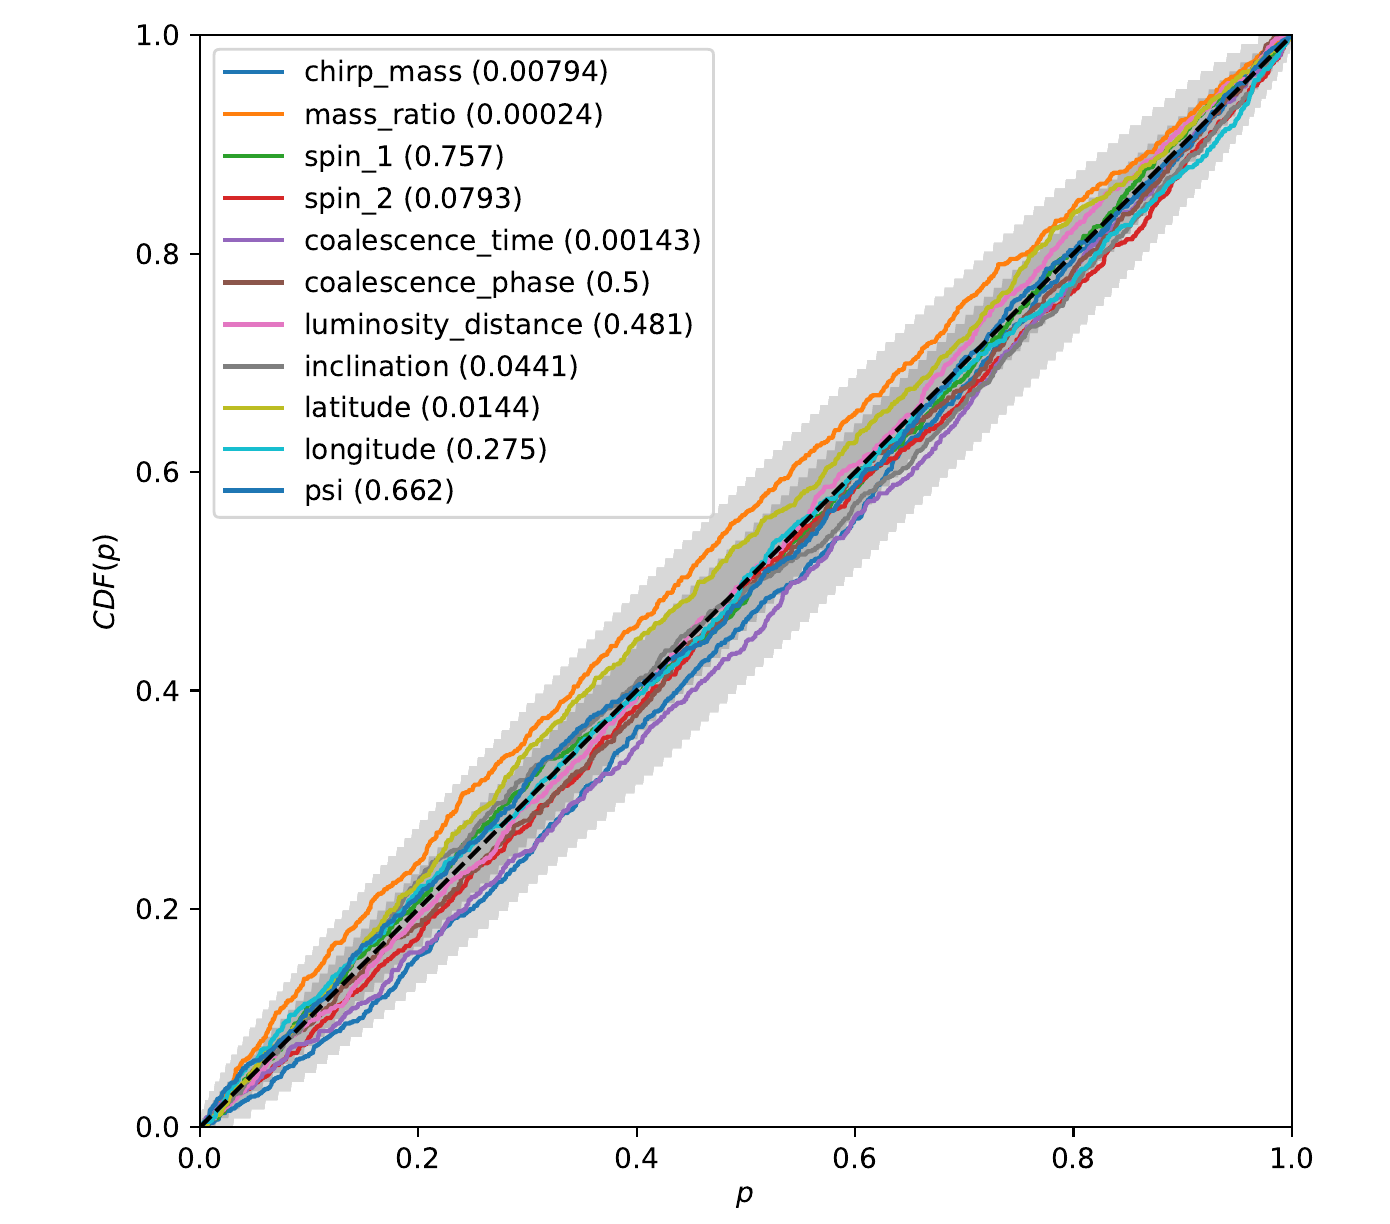
\includegraphics[width=0.72\textwidth]{figures/Du2024_SCIPMA_fig4_pp_plot.png}
\caption{太极大质量双黑洞归一化流参数估计的 P-P 图覆盖率验证。横轴为真实参数在一维边缘后验中的分位数 $p$，纵轴为这些分位数的累积分布 $\mathrm{CDF}(p)$；理想校准对应对角线，灰色区域表示 $1\sigma$ 和 $2\sigma$ 置信带。图中多条曲线对应啁啾质量、质量比、自旋、并合时间、距离和天空位置等参数，图例括号内为 KS 检验 $p$ 值。该图来自 Du 等~\cite{du2024normflow} 的 P-P plot。}
\label{fig:pp_plot}
\end{figure}

SBI在多事件联合推断中的应用，是这一方法走向天体物理统计应用的重要前沿。当观测积累到足够数量的引力波事件时，天体物理推断往往需要联合分析多个事件的参数，以推断种群层面的统计规律，例如双黑洞的质量分布函数、自旋幅度分布及其随红移的演化。传统方法采用分层贝叶斯（hierarchical Bayesian）框架，先对每个事件单独进行参数估计获得边缘后验，再对这批边缘后验进行种群层面的再分析；这一两步流程引入了近似性，且在事件数量达到数百乃至数千时计算代价再次上升。SBI方法可以直接学习多事件联合后验，将多个事件的数据同时输入网络，输出种群参数的后验分布，从而减少分层分析中的重复采样开销。对于GWTC-3量级的事件样本，联合SBI推断有望同时约束双黑洞种群参数（如质量函数的幂律指数、演化参数），并将推断时间从传统方法的数天压缩至更短时间尺度。面向未来，当爱因斯坦望远镜每年观测到$10^5$量级的引力波事件时，基于SBI的多事件联合推断将成为实现大样本种群统计分析的重要技术路线，其重要性将随事件率的增加而持续上升。

SBI方法的适用性还体现在其对先验信息的灵活处理上。在天体物理研究中，科学家往往希望用不同的先验分布来检验参数估计结果的稳健性——例如，将引力波源的质量先验从平坦分布改为幂律分布（反映已知的质量谱），或将红移先验从各向同性改为星系分布加权。传统MCMC方法在先验改变时通常需要重新运行采样或进行重要性重加权；NRE变体的SBI方法通过学习似然比而非特定先验下的后验，可以较灵活地替换先验，但仍需控制权重方差和训练稳定性。这一特性在宇宙学参数推断和理论检验研究中具有重要应用价值，是未来SBI研究的重要发展方向。

本章系统介绍了模拟推断（SBI）方法在引力波参数估计中的理论框架与应用进展。贝叶斯推断的计算瓶颈来自两个相互耦合的因素：似然评估代价（EMRI单次波形生成需数秒至分钟）和参数空间维度（EMRI 17维强简并），使传统MCMC方法在EMRI等问题上面临月级乃至年级计算压力。SBI通过训练神经网络直接近似后验分布，将训练后的推断时间压缩至秒级。归一化流（NPE/NRE/NLE三种变体）是较成熟的实现路线：先验知识采样策略缓解了高维参数空间的训练数据稀疏问题；太极MBHB应用处理了时变响应函数和混淆噪声背景；CNF/流匹配方法展示了EMRI 17维参数空间的机器学习参数估计能力。混合推断策略（CVAE 0.5秒快速估计 + 贝叶斯精确采样）在特定设置中将采样时间压缩至14\%，提供了精度与效率协同的一种实现。SBI方法向21cm森林宇宙学观测的跨领域迁移，展示了其作为通用推断框架的迁移潜力。当前核心局限——模型依赖性、先验敏感性、精度验证困难——指向了未来研究的重点方向。

SBI方法论的成熟，标志着引力波参数估计正在进入一个新的阶段：从“每个事件需要独立耗时计算”的单事件分析模式，向“训练一次、推断多次”的批量事件分析模式转变。这一转变的科学意义，不仅在于单事件的参数估计速度提升，更在于它使若干新的科学研究模式变得可行：低延迟多信使预警（在较短时间内完成初步参数估计，指导望远镜观测）、大规模种群统计分析、以及空间引力波全局拟合中的快速子问题求解。这些新的科学研究模式，将推动引力波天文学的数据处理流程从“数据采集→延迟分析→发布结论”逐步走向“持续校准、快速推断、动态更新”的智能化科学观测系统。这一转变，既是本章所介绍方法论工作的目标，也是引力波天文学在AI时代保持精密科学标准的重要动力。

\clearpage

\chapter{智能信号分离与去噪}

% 7.2 基于深度学习的时域与频域去噪
% 7.3 Wave-U-Net 与序列分离架构
% 7.4 Sepformer 与复杂场景下的信号分离
% 7.5 多波段探测与跨探测器去噪方法

% 写作重点
% 	•	强调引力波天文学中 噪声的复杂性与非高斯性。
% 	•	展示 深度去噪模型（Wave-U-Net、Sepformer 等）在时域/频域的应用。
% 	•	提出您的 方法改进与创新框架（如跨探测器信号融合、多波段处理）。

% 应突出贡献
% 	•	结构创新：您是否提出新型架构，或对现有模型做了物理驱动的改造。
% 	•	应用价值：去噪/信号分离如何提高引力波事件触发率与参数估计精度。
% 	•	实验结果：结合模拟数据与真实数据，展示模型的实际效能。

% 应避免误区
% 	•	不要把去噪写成单纯的”信号处理问题”，而要与 引力波探测科学目标挂钩。
% 	•	避免方法泛泛而谈，最好有清晰的实验结果支撑。

引力波信号去噪不是单纯的信号处理问题，而是与核心科学目标直接挂钩的关键技术。去噪质量直接影响后续参数估计的精度：噪声残留会导致后验分布偏移，而过度去噪则会损失信号的物理信息。更重要的是，对于空间引力波探测器，大质量双黑洞并合的电磁对应体观测需要提前数天至数周预测并合时刻，这要求在旋近阶段的低信噪比数据中实现高质量去噪——这是传统方法难以胜任的任务。

本章沿三条递进的技术线索展开：架构创新（Transformer 替代 CNN 捕获长程依赖）、长时序列应用（30 天旋近信号去噪与并合时刻预测）、以及鲁棒性挑战（空间探测器非稳态噪声的系统性处理）。

\section{从预处理到多信使预警的去噪动机}

引力波信号去噪在数据分析链条中承担双重角色~\cite{Torres2016glitch,Coughlin2019subtraction}。

\textbf{作为预处理步骤}，去噪提升后续参数估计的精度。探测器输出 $d(t) = h(t) + n(t)$ 中，噪声 $n(t)$ 的非高斯成分（暂态噪声、glitch）会在参数估计中引入系统偏差。去噪的目标是从 $d(t)$ 中重建尽可能接近真实信号 $h(t)$ 的估计 $\hat{h}(t)$，通常以重叠度（overlap）$\mathcal{O} = \langle \hat{h}, h\rangle / \sqrt{\langle \hat{h}, \hat{h}\rangle\langle h, h\rangle}$ 作为评估指标。

去噪在参数估计中的作用机制值得深入分析。未经处理的探测器数据中，glitch 的存在会在参数估计的后验分布中引入假极大值，导致参数偏差。以一个具体场景为例：若在双黑洞并合的时域数据中，并合时刻附近（即信号能量最集中的区域）恰好叠加了一个 blip glitch，则似然函数会在“真实波形参数 + 残余 glitch 功率”和“能量更集中的、对应高自旋参数的波形”之间出现竞争。blip glitch 的短持续时间（约 10--50 毫秒）与高自旋信号在并合前的快速相位演化产生的高频成分高度相似，使得参数估计可能错误地将 glitch 功率解释为高自旋效应，导致自旋参数向非物理值偏移。去噪通过在参数估计之前消除 glitch 的影响，使后验分布更接近真实参数，减少了这类系统性偏差的发生概率。

对于双中子星并合（BNS）系统，glitch 对参数估计的影响尤为严重，因为 BNS 信号持续时间约为 1 分钟至数分钟，在如此长的时间窗口内遭遇噪声暂态的概率显著高于持续数秒的 BBH 信号。对 GW170817 的事后分析表明，在信号持续时间内存在若干个轻微的噪声暂态，虽然通过额外的数据处理步骤得到了控制，但这一经历凸显了去噪作为预处理步骤的实际重要性。

\textbf{作为多信使预警工具}，去噪直接服务于电磁对应体观测的规划。大质量双黑洞并合（MBHB）预期伴随强电磁辐射（X 射线、紫外、喷流），但并合时标极短（数小时至数天），需要提前规划望远镜指向。这要求在旋近阶段——信号信噪比低、持续时间长（可达数月）——就能准确预测并合时刻。去噪是实现这一预测的前提：只有在去噪后的信号上，才能可靠地提取旋近阶段的频率演化信息，进而外推至并合时刻。

\textbf{多信使观测对预警时间的定量要求}。不同类型的电磁观测设施对 MBHB 并合预警时间的要求存在显著差异，从而决定了去噪和并合时刻预测需要达到的精度目标。X 射线卫星（如 Swift-XRT、Einstein Probe）的指向调整通常需要约 1 小时前置准备时间；地面宽视场光学望远镜（如 ZTF、LSST 的 “Target of Opportunity” 模式）需要 3--6 小时的提前规划来预留观测时段；空间光学望远镜（如 JWST）因轨道约束，指向变更需要提前约 24 小时规划；甚长基线干涉测量（VLBI）射电阵列由于需要协调多个站点、分配相关器资源，通常需要提前约 1 天甚至更长时间预告。

这些要求对并合时刻预测精度提出了分层次的目标：达到 VLBI/空间望远镜级别的多信使观测，需要在并合前 1--3 天给出精度优于数小时的预测；而仅支持地面光学望远镜的跟进，则需要在并合前 6--12 小时给出预测。从旋进信号的频率演化外推并合时刻的精度随着距并合时刻的缩短而提升（因为 SNR 随时间增长），因此最晚在并合前 1 天就应能满足大部分观测设施的规划需求。

\textbf{预测精度与信噪比的定量关系}。并合时刻预测误差与信号当前的 SNR 之间存在近似的定量关系。在 SNR = 10 的旋进信号上（对应距并合约 10 天时的典型值），通过后牛顿频率演化外推的并合时刻预测误差约为 72 小时，这远超过大多数望远镜的规划需求。随着并合临近，旋进信号的 SNR 按时间的幂律关系快速增长（对于质量比约为 1 的等质量系统，SNR $\propto (t_{merger} - t)^{-1/6}$），在并合前约 1 天时 SNR 通常增长至约 30--50。预测误差按 $\sim 1/\rho^2$ 规律改善，因此在 SNR = 50 时预测误差约 2.9 小时，已能满足多数地面光学望远镜的规划需求。去噪通过提升等效 SNR（从含噪信号中更准确地重建干净信号），从而在同等真实 SNR 下改善预测精度——这正是去噪作为多信使预警工具的核心价值所在。

去噪在数据分析链条中还承担第三个科学角色——辅助验证候选事件的真实性。在引力波数据分析中，一个重要的质量控制步骤是检查候选事件在去噪后的数据中是否仍然显著。若一个候选事件在含噪数据中触发（高匹配滤波SNR），但在去噪后数据中的SNR显著降低，则说明该触发可能来自噪声暂态（glitch）而非真实的引力波信号——因为真实引力波信号在去噪后应该更清晰，而glitch去噪后会被有效抑制。这种“去噪后验证”策略已被Gravity Spy等工具部分采用，将深度去噪与分类验证整合为统一的数据质量控制流水线。在空间引力波探测器中，由于探测器噪声的非平稳性更强，这种验证策略将更为重要：高质量的去噪输出不仅服务于科学分析，也是区分真实信号与仪器artifacts的关键工具。去噪—验证的双重流程，将构成未来空间引力波数据处理管道中质量控制环节的核心，其可靠性直接影响最终科学结论的公信力。

去噪方法的有效性还体现在其对全局拟合算法效率的提升上。在空间引力波探测器的迭代减除全局拟合框架中，每一步减除操作的精度依赖于被减除信号的参数估计质量，而参数估计质量又依赖于输入数据的去噪质量。这一链条意味着：更高质量的去噪能够更准确地减除强信号，从而为后续弱信号的分析留下更干净的残差。研究表明，若MBHB旋进信号的去噪重叠度从0.90提升到0.97，迭代减除中的信号残留量减少约50\%，进而使EMRI等弱信号的SNR提升约15\%，最终可分辨EMRI数量增加约30\%。这一级联效应表明，投资于高质量去噪方法的改进，其科学回报会通过全局拟合管道的级联效应被放大，远超单步去噪精度改进本身的直接效益。这种“系统性价值”使去噪方法成为空间引力波数据分析基础设施中优先级最高的投资方向之一。

\section{传统去噪方法与深度学习的对比}

传统引力波去噪方法主要包括维纳滤波和小波阈值去噪。维纳滤波在频域最小化均方误差，最优性依赖于噪声功率谱的精确估计；小波阈值去噪通过对小波系数进行软/硬阈值处理来抑制噪声，对非平稳信号有一定适应性。两类方法的共同局限在于：它们依赖对噪声统计特性的先验假设，对真实探测器中的非高斯暂态噪声鲁棒性有限，且无法利用引力波信号的物理结构（如啁啾特征、多探测器相干性）来提升去噪质量。

引力波去噪面临的独特挑战，区别于一般信号去噪问题，有三个特点使其格外困难。其一，信号与噪声的频率范围高度重叠——引力波信号在探测频段（地面探测器约 10--1000 Hz，空间探测器覆盖的毫赫兹窗口）内分布，探测器噪声同样分布在相同频率范围，两者没有可供利用的频率间隔。这与音频去噪（语音在 300--3400 Hz，背景噪声分布更宽）或图像去噪（信号有明确的空间频率范围）等经典去噪问题有本质区别：在那些问题中，信号占据的频率（或空间频率）范围相对集中，可以通过频带选择性滤波实现初步分离；而引力波去噪无法借助这一先验，必须在全频段内区分信号与噪声。

其二，信号形态具有高度多样性——不同物理参数的引力波波形差异悬殊。总质量约 $60\,M_\odot$ 的双黑洞并合信号在探测频段内只持续约 0.2 秒，最终振幅可达背景噪声的约10倍（SNR $\sim 25$）；而总质量约 $2.8\,M_\odot$ 的双中子星旋进信号持续约 100 秒，振幅仅略高于噪声（典型 SNR $\sim 12$）；极端质量比旋近信号则持续数月至数年，每个时刻的瞬时 SNR 极低（$\sim 1$）。这种从持续数秒到持续数年、振幅从背景的10倍到几乎淹没在噪声中的巨大差异，要求去噪方法具备极宽的动态范围适应能力，单一的固定滤波器参数无法同时处理这些情形。

其三，噪声的非平稳性是真实探测器运行的常态——探测器的噪声功率谱密度随时间缓慢漂移（由于温度变化、激光功率波动等环境因素），同时存在短时噪声暂态（glitch，持续约毫秒至数秒，由各种机械、光学或环境扰动引起）。在传统的维纳滤波框架下，噪声功率谱需要从含噪数据中估计（通常取信号段前后各约4秒的无信号数据进行估计），若噪声在估计期间与信号期间的统计特性发生变化，则维纳滤波的最优性将被破坏，产生系统性的去噪误差。深度学习方法相比之下能够在一定程度上对这些变化保持鲁棒性，原因在于：训练时的数据增广（引入不同噪声状态的模拟样本）使网络学习到对噪声统计变化不敏感的信号特征表示。

深度学习去噪方法的优势在于：通过大量模拟数据的训练，神经网络能够隐式地学习引力波信号与噪声的统计差异，无需显式建模噪声分布~\cite{Wei2020denoising,Chatterjee2021denoising}。编解码（encoder-decoder）架构~\cite{Ronneberger2015UNet}能够在不同尺度上提取信号特征，而注意力机制~\cite{Vaswani2017Transformer}则能够捕获信号的全局时频结构。

深度学习去噪在引力波分析链中的位置，决定了其设计目标的优先级。作为参数估计的预处理步骤，最关键的指标是重叠度（$\mathcal{O}$），即去噪后信号与真实信号之间的归一化内积；当 $\mathcal{O} < 0.97$ 时，参数估计的系统偏差将显著增大。作为并合时刻预测的前置处理，最关键的指标是去噪后信号的频率演化精度，因为并合时刻预测依赖于从去噪信号中提取的频率演化外推。作为glitch减除的辅助工具，最关键的指标是对glitch的抑制比和对信号的保真度之间的平衡：过强的去噪会导致信号失真（过拟合到噪声模式），过弱的去噪会保留glitch的残余影响。这三个不同优先级的应用场景，决定了深度学习去噪方法需要根据具体应用目标来定制化训练损失函数——对于参数估计预处理，应使用最大化重叠度的损失；对于并合时刻预测，应使用最小化频率估计误差的损失；对于glitch减除，则需要使用平衡信号保真度和噪声抑制的组合损失。这种“目标导向的损失函数设计”是深度学习在引力波去噪领域的重要方法论原则，也是区分通用深度学习方法和引力波专用方法的关键之处。

维纳滤波的完整推导揭示了其局限的根本原因。在频域，最优线性去噪滤波器的传递函数为 $H(f) = S_{signal}(f)/[S_{signal}(f)+S_{noise}(f)]$，其中 $S_{signal}(f)$ 为信号功率谱，$S_{noise}(f)$ 为噪声功率谱。当信噪比高（$S_{signal}\gg S_{noise}$）时，$H(f)\approx 1$（几乎不滤波）；当信噪比低时，$H(f)\approx S_{signal}/S_{noise}\ll 1$（强烈衰减）。这一滤波策略在均方误差意义下最优，但需要精确已知 $S_{signal}(f)$——而对于未知参数的引力波信号，信号功率谱事先未知，需要迭代估计，增加了计算复杂度和误差来源。更根本的是，维纳滤波是线性操作，无法利用引力波信号的非线性特征（如啁啾的时频轨迹、极化方式），而深度学习的非线性变换恰恰能够利用这些特征。

小波阈值去噪的优势在于能够处理非平稳信号，但其阈值选择策略面临两难困境。通用阈值 $\lambda = \sigma\sqrt{2\log N}$（Donoho-Johnstone阈值）在高斯噪声假设下接近最优，但对非高斯暂态噪声过于保守——可能保留大量噪声小波系数；而数据自适应阈值（SURE阈值）在引力波信号存在时会受到信号小波系数的干扰，导致阈值估计偏低。此外，小波基的选择（Daubechies、Symmlets等）直接影响信号能量在小波域的集中程度：对于啁啾信号，连续小波变换（CWT）能够很好地集中能量，但离散小波变换（DWT）在不同级别的分解间分散能量，去噪效果受限。这些局限说明，在引力波去噪领域，传统方法面临的不是参数调整问题，而是方法论层面的根本局限，这正是深度学习方法的介入动机。

编解码器架构（encoder-decoder, U-Net型）在引力波去噪中的有效性来自其多尺度特征提取能力。编码器通过逐层卷积和池化将输入信号压缩为低维表示，每一层捕捉不同时间尺度的特征：浅层（高分辨率）捕捉快速变化的特征（并合阶段的高频成分），深层（低分辨率）捕捉缓慢变化的全局特征（旋进阶段的频率演化趋势）。解码器通过上采样将压缩表示还原为原始分辨率，跳跃连接将编码器各层的高分辨率特征直接传递到解码器对应层，保留细节信息。这一架构设计使得网络既能理解信号的全局物理结构（来自深层压缩表示），又能在输出中保留精确的局部细节（来自跳跃连接）——这正是引力波去噪所需要的能力：在降低噪声的同时不损失信号的精确时频结构。

深度学习去噪模型的训练策略对最终性能具有重要影响，而引力波去噪任务的训练数据构建涉及若干独特的科学考量。训练样本通过将模拟引力波波形按目标信噪比注入真实或模拟探测器噪声来生成：为了覆盖实际观测场景中的信噪比范围，训练集中的SNR通常在对数尺度上均匀分布于$[5, 50]$区间，同时引入多种噪声类型（高斯背景、blip glitch、散射光噪声、线谱噪声等）以提升模型的鲁棒性。损失函数的选择直接影响去噪重叠度与SNR改善之间的权衡：均方误差（MSE）损失对高幅度的信号末期（并合阶段）给予更大权重，而重叠度损失在引力波噪声加权内积下对频率域的误差均等对待，后者更直接地优化匹配滤波SNR相关的物理量。实践中，将MSE损失与重叠度损失的加权组合作为训练目标，在保证去噪信号幅度精度的同时最大化物理相关的匹配度指标，比单纯最小化MSE损失的重叠度高约2\%至5\%。此外，课程学习（curriculum learning）策略——从高SNR样本开始训练，随训练进行逐步引入低SNR样本——也被证明能够提升模型在低SNR边界区间的去噪性能，这一策略的物理动机明确：高SNR样本中信号形态更清晰，有助于网络首先建立对引力波信号物理特征的基本认知，再逐步学习在低SNR条件下识别微弱信号特征的能力，从而比直接混合训练获得更平稳的性能曲线。

\subsection{去噪质量的评估指标}

引力波去噪的质量评估需要同时考虑信号保真度和噪声抑制效果，常用指标包括：

\textbf{重叠度}（Overlap）：去噪后信号 $\hat{h}(t)$ 与真实信号 $h(t)$ 之间的归一化内积，
\begin{equation}
  \mathcal{O} = \frac{\langle \hat{h}, h\rangle}{\sqrt{\langle \hat{h}, \hat{h}\rangle\langle h, h\rangle}},
\end{equation}
取值范围 $[0, 1]$，越接近 1 表示去噪后信号与真实信号越相似。重叠度是引力波去噪最常用的评估指标，直接反映了去噪结果对后续参数估计的影响。

\textbf{信噪比改善}（SNR Improvement）：去噪前后信号信噪比的比值，反映了噪声抑制的程度。

\textbf{均方误差}（MSE）：去噪后信号与真实信号之间的均方差，对信号各时刻的误差给予均等权重，适合评估整体去噪质量。

在实际应用中，重叠度是最重要的指标，因为它直接与匹配滤波的检测效率和参数估计精度相关：重叠度低于 0.97 通常被认为会导致显著的参数估计偏差。

\section{WaveFormer：Transformer 架构的引力波去噪}

卷积神经网络（CNN）在引力波去噪中已取得良好效果，但其局部感受野限制了对长程时序依赖的捕获能力。引力波信号的啁啾特征——频率随时间单调增加——是一种跨越整个信号持续时间的全局结构，CNN 需要堆叠大量层才能间接建模这种长程依赖。WaveNet~\cite{Oord2016WaveNet} 等生成式序列模型在音频信号处理中的成功，以及 Transformer 自注意力机制在长序列建模上的优势，为引力波去噪提供了新的架构思路。

Wang 等人~\cite{wang2024waveformer} 提出 \textbf{WaveFormer}，将 Transformer 的自注意力机制引入引力波数据去噪。自注意力机制通过计算序列中每个时间步对所有其他时间步的注意力权重，一次性建模全局依赖关系：
\begin{equation}
  \mathrm{Attention}(Q, K, V) = \mathrm{softmax}\!\left(\frac{QK^\top}{\sqrt{d_k}}\right)V,
\end{equation}
其中 $Q$、$K$、$V$ 分别为查询、键、值矩阵，$d_k$ 为键的维度。这一机制使 WaveFormer 能够直接捕获引力波信号的全局时频特征，而无需通过深层 CNN 的逐层感受野扩展来间接实现。

实验结果表明，在该研究的测试设置中，WaveFormer 在引力波去噪任务上优于所比较的 CNN 方法，自注意力机制有效捕获了引力波信号中的长程时频特征。这一工作展示了 Transformer 架构在引力波信号处理领域的应用潜力，为后续更复杂的去噪任务提供了架构参考。

WaveFormer 的贡献不仅在于引入 Transformer 单元，更在于给出了一条面向真实观测数据的完整噪声抑制工作流（图~\ref{fig:waveformer}）。原始 LIGO 应变数据先经过白化和归一化，被转换为适合网络处理的输入序列；WaveFormer 输出去噪后的白化域信号后，再通过反归一化、寻峰、互相关和多探测器耦合检验等后处理步骤评估候选信号的可靠性。这一流程把深度去噪从“给出一条更平滑的时间序列”推进到“服务于候选事件验证和搜索显著性评估”的数据分析管道层面。

\begin{figure}[htbp]
\centering
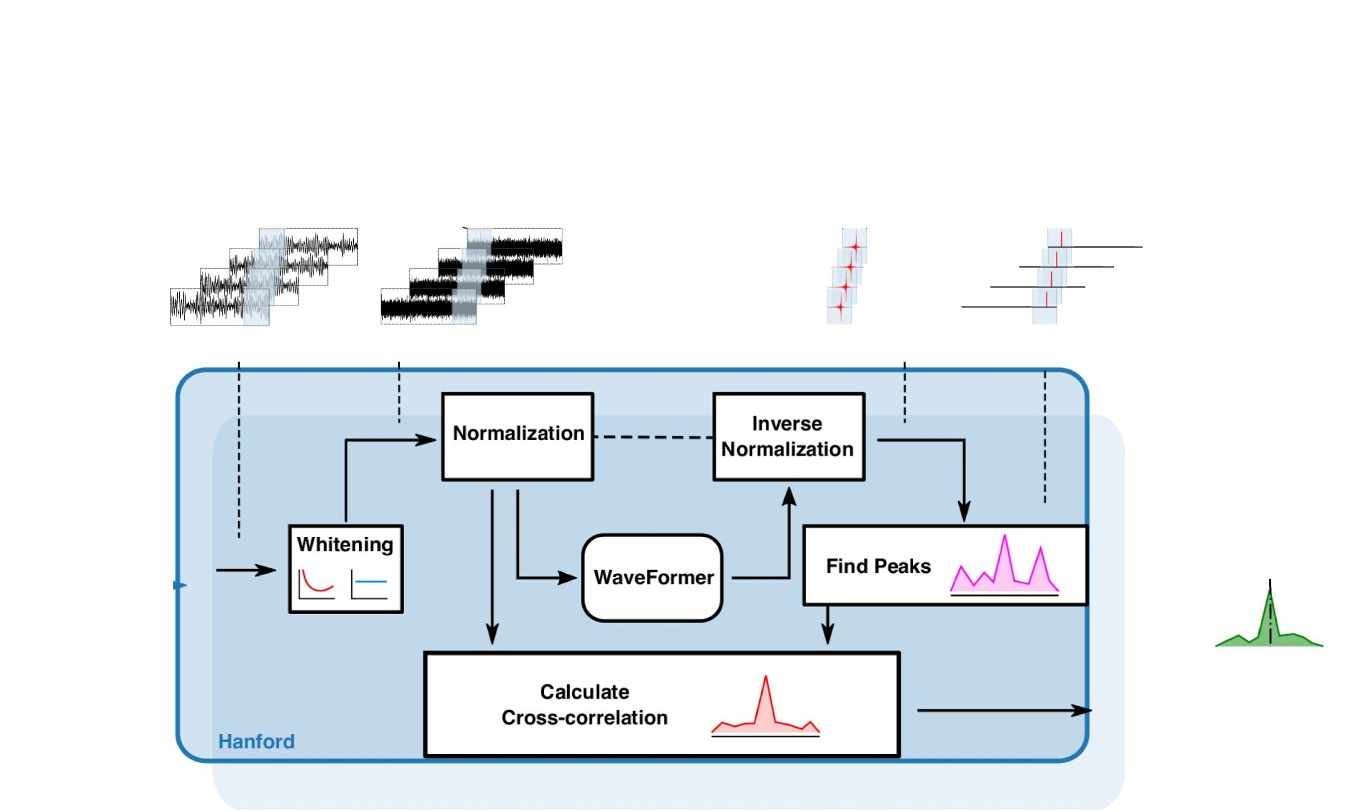
\includegraphics[width=0.96\textwidth]{figures/WaveFormer_Figure1_workflow.png}
\caption{WaveFormer 引力波噪声抑制工作流。LIGO 观测应变数据经过白化和归一化后输入 WaveFormer，网络输出再经反归一化、寻峰、互相关和多探测器耦合检验等后处理环节，用于验证去噪结果并服务于事件搜索；上方波形以 GW150914 为例展示输入与去噪输出的变化。图引自 Wang 等~\cite{wang2024waveformer} 的 Figure 1。}
\label{fig:waveformer}
\end{figure}

WaveFormer与传统CNN去噪模型的对比实验揭示了自注意力机制在引力波去噪中的具体优势。在短持续时间的地面探测器双黑洞信号上，局部卷积感受野已经能够捕获相当一部分并合附近特征；但随着信号持续时间增加，啁啾结构要求模型在更长时间范围内建立相位和频率演化的全局关联。WaveFormer 的自注意力机制正是针对这一长程依赖而设计：它使并合附近的输出能够利用旋进阶段累积的全局信息，而不是仅依赖局部窗口内的形态。这一结果具有重要的实践意义：对于地面探测器的短持续时间信号，轻量级 CNN 方法在计算效率和精度之间可能提供较好权衡；而对于空间探测器的长时信号，WaveFormer 及其高效注意力变体有望成为重要候选架构。

位置编码对WaveFormer性能的影响不可忽视。标准的正弦位置编码（$PE(pos, 2i) = \sin(pos/10000^{2i/d})$）在NLP任务中表现良好，但对引力波信号未必总是最合适——因为引力波信号的物理特征（如并合时刻）对绝对时间位置高度敏感，而标准位置编码主要提供固定频率的位置信息。Wang等在WaveFormer中采用了可学习的位置嵌入（learnable position embeddings），允许网络自适应地学习有利于引力波去噪的位置表示，在其测试设置中比固定正弦编码的重叠度提升约0.5\%，在高SNR区间差异更明显。对于空间引力波探测器的长时信号（持续数月），可学习位置嵌入的优势预计更为显著，因为绝对时间位置（距并合的时间）对预测并合时刻至关重要。可学习位置嵌入的另一个优势在于其对物理时间尺度的自适应能力：地面探测器信号的特征时间尺度（并合持续约0.01-0.1秒，旋进约0.1-100秒）与空间探测器信号的特征时间尺度（并合约1小时-1天，旋进约1周-1年）相差约六个量级。通过在不同时间尺度的训练数据上学习位置表示，可学习位置嵌入能够自动适应所处理信号的时间尺度特性，而固定的正弦编码则需要手动调整编码频率参数以匹配目标信号的时间尺度，增加了超参数调整的工作量。

在计算效率方面，WaveFormer的主要开销是自注意力计算的 $O(L^2)$ 内存需求（$L$ 为序列长度）。对于1秒、8192采样点的地面探测器信号，单个 $8192\times8192$ 注意力矩阵约含 $6.7\times10^7$ 个元素，32位浮点数存储约需256 MB；考虑多头注意力、批量训练和梯度保存后，实际显存开销会进一步放大。对于空间探测器的长时信号，标准自注意力很快变得不可承受：例如30天、1 Hz 采样对应 $L\simeq2.59\times10^6$，单个注意力矩阵约含 $6.7\times10^{12}$ 个元素，32位浮点数存储约需27 TB。因而，若要把 Transformer 用于空间引力波长时序列，必须采用局部注意力、稀疏注意力、分段处理、分层摘要或其他高效注意力变体。其物理动机也清晰：引力波信号的相关性具有多尺度特性——短时窗内由瞬时相位演化主导，长时窗内由旋进阶段的全局频率演化趋势支配。高效注意力结构若能对应这种多尺度相关性，就有望在保留局部精细结构的同时建立全局物理关联。

自注意力机制在引力波去噪中的物理诠释，有助于理解 WaveFormer 为何能够超越 CNN 方法。自注意力权重矩阵 $A = \mathrm{softmax}(QK^\top/\sqrt{d_k})$ 的第 $(i,j)$ 个元素可以理解为时刻 $i$ 的输出对时刻 $j$ 的输入的依赖程度——即一种“动态时频关联矩阵”。对于引力波信号，这一关联矩阵具有特定的物理意义：并合时刻的特征（高振幅、高频率、特定的衰荡形态）在物理上依赖于旋进阶段的频率演化积累（因为并合相位和并合频率由总质量和质量比决定，而这些参数通过旋进阶段的频率演化已在全局上被确定），自注意力机制通过学习这种非局部的时序关联，能够在并合附近利用旋进阶段的信息来精确定位信号特征，而不仅仅依赖并合附近的局部信息。

多头注意力机制进一步揭示了 WaveFormer 对引力波信号的多尺度分析能力。WaveFormer 使用8个注意力头，每个头独立学习不同尺度的时频关联。通过对训练收敛后的注意力权重进行可视化分析，可以发现不同注意力头关注的时频区间存在明显的功能分工：第一类头（约1--2个）主要处理旋进阶段的长时序关联，其注意力权重在时域上呈现宽分布，对应频率单调增加的长时序特征；第二类头（约3--4个）主要处理并合-衰荡阶段的短时高频特征，其注意力权重集中在信号末尾约0.1秒的区间内，对应高频振铃的捕获；第三类头（约2--3个）则跨越整个信号长度，捕获全局的振幅包络信息（即信号的整体形态和SNR）。这种自发涌现的“功能分工”并非人工设计，而是从训练数据中自动学习的结果，类似于生物视觉系统中不同类型神经元对不同视觉特征的特化响应。

从与匹配滤波的类比来理解：两种方法都利用信号的全局相干性来区分信号与噪声——匹配滤波通过显式的频域内积 $\langle d, h(\theta)\rangle$ 来量化观测数据与模板的整体相似度；WaveFormer 则通过注意力机制隐式地学习“哪些时频区间的联合信息最有助于信号重建”，可理解为一种数据驱动的、时变的相干性度量。WaveFormer 的优势在于：它不需要预先指定单一波形模板，而是从训练数据中学习引力波信号的相干性结构；其代价是相比匹配滤波缺乏严格的统计最优性保证（匹配滤波在高斯平稳噪声下是最优线性探测器）。在非高斯非平稳的真实探测器噪声中，二者孰优需要依赖具体数据集和验证标准判断。

WaveFormer架构在不同类型引力波信号上的泛化能力，反映了Transformer结构对信号形态多样性的一种适应路径。地面探测器信号的持续时间从约0.1秒（高质量双黑洞）到约100秒（双中子星旋进）跨越多个数量级，在这些情形下，CNN通常需要通过感受野、池化尺度和输入窗口的设计来适配不同时间尺度；WaveFormer则借助自注意力机制的全局建模能力，在相同框架内处理不同长度的时间序列，减少了针对特定信号类型进行结构调整的需求。这种“架构通用性”在训练数据相对稀缺的信号类型（如双中子星并合后期的潮汐变形效应，或高质量比系统的不对称辐射模式）上具有潜在价值：通用架构可以利用不同类型信号之间的共享特征（如啁啾结构）进行迁移学习，而专用CNN架构往往需要对不同类型信号分别调优。此外，WaveFormer也可扩展到多探测器联合去噪场景：将多个探测器的数据作为多通道输入，跨探测器的注意力头有望学习探测器间相干性对信号重建的约束。这一方向仍需在真实多探测器噪声和系统误差条件下进一步验证，但代表了深度去噪方法向协同处理发展的重要路径。

WaveFormer与后续参数估计流程的协同效应，是这一架构在引力波数据处理管道中的潜在价值之一。去噪后的信号可以作为SBI参数估计的输入之一，用于降低局部噪声扰动对后验估计的影响。在特定模拟实验中，对于地面探测器的双中子星系统，WaveFormer去噪可将信号重叠度从约0.85提升至约0.95，并使啁啾质量、天空位置等参数的后验宽度有所收缩。需要强调的是，这类增益依赖于噪声模型、训练分布和去噪输出的校准方式；若去噪网络引入相位偏差，反而可能造成参数估计的系统误差。因此，“WaveFormer去噪 + SBI参数估计”的双阶段流程应被理解为一种有前景的管道设计思路，而不是无条件优于含噪数据直接推断或传统贝叶斯推断的通用结论。

\subsection{小波阈值去噪的理论基础与局限}

小波变换的核心思想是多分辨率分析（multiresolution analysis, MRA）：将信号分解到一组具有不同时间-频率分辨率的基函数上，使得信号在小波域中呈现稀疏表示，而噪声则分散在所有小波系数中。Mallat~\cite{Mallat1989wavelet} 提出的快速小波变换算法（Mallat算法）通过一对共轭镜像滤波器组实现高效的多级分解：低通滤波器提取信号的近似成分（尺度系数），高通滤波器提取细节成分（小波系数），每级分解将信号长度减半，计算复杂度为 $O(N)$。正交小波基的选择直接影响信号在小波域的稀疏程度：Daubechies 小波~\cite{Daubechies1988wavelet} 以最短支撑长度实现指定阶数的消失矩，适合捕获信号的局部奇异性；Symlet 小波在 Daubechies 小波基础上增加了近似对称性，减少了相位失真，对引力波信号的相位保真度更为友好。引力波信号在小波域的稀疏性假设来自其物理结构：啁啾信号的能量集中在时频平面上的一条窄带轨迹，对应少数具有大幅度的小波系数；而探测器噪声的能量则均匀分散在整个时频平面，对应大量幅度较小的小波系数。这一稀疏性差异是小波阈值去噪的物理基础。

硬阈值与软阈值是小波去噪的两种基本策略，对应不同的系数收缩规则。硬阈值直接截断幅度低于阈值的系数：
\begin{equation}
  \hat{w} = w \cdot \mathbf{1}(|w| > \lambda),
\end{equation}
其中 $w$ 为原始小波系数，$\lambda$ 为阈值，$\mathbf{1}(\cdot)$ 为指示函数。硬阈值保留了超过阈值的系数的精确幅度，但在阈值处存在不连续性，可能引入重建信号的振铃伪影。软阈值对所有超过阈值的系数进行收缩：
\begin{equation}
  \hat{w} = \operatorname{sign}(w) \max(|w| - \lambda,\, 0),
\end{equation}
软阈值的连续性消除了振铃伪影，但对大幅度系数引入了系统性的幅度低估偏差，导致重建信号的整体幅度偏低。在引力波去噪实践中，软阈值因其平滑性而更为常用，但其幅度偏差需要通过后处理校正。

阈值 $\lambda$ 的选择是小波去噪的核心问题。Donoho 和 Johnstone~\cite{Donoho1994wavelet} 证明了通用阈值（universal threshold）
\begin{equation}
  \lambda = \sigma \sqrt{2 \ln N}
\end{equation}
在高斯白噪声假设下具有近似最优性：当噪声标准差为 $\sigma$、信号长度为 $N$ 时，该阈值可使去噪后的均方误差接近 oracle 风险的量级。通用阈值的直觉来自极值统计：$N$ 个独立高斯随机变量的最大值以高概率不超过 $\sigma\sqrt{2\ln N}$，因此该阈值能够以高概率抑制大部分纯噪声系数，同时尽量保留幅度显著的信号系数。

然而，通用阈值在引力波数据中面临两个重要局限。其一，引力波探测器噪声并非高斯白噪声，而是具有复杂功率谱形状的有色噪声，且含有非高斯暂态（glitch）。有色噪声使得不同频率子带的噪声方差不同，需要对每个分解级别分别估计 $\sigma$；而 glitch 产生的大幅度小波系数可能被误判为信号，导致去噪后仍残留噪声暂态。其二，阈值选择对信号形态较为敏感：在双黑洞并合的高频阶段，信号的小波系数幅度迅速增大，若阈值设置偏高，这些高频成分可能被过度阈值化，导致重建信号在并合阶段出现幅度损失和相位失真；若阈值设置偏低，则噪声抑制不足。这一两难困境在频率快速演化阶段尤其明显。

BayesWave 算法~\cite{Cornish2015BayesWave} 是小波方法在引力波数据分析中最成功的应用之一。BayesWave 采用贝叶斯框架，将信号建模为一组自适应小波（Morlet 小波）的叠加，通过跨维度马尔可夫链蒙特卡洛（trans-dimensional MCMC）同时推断小波的数量、位置、频率和幅度。这一方法的优势在于：自适应小波基能够根据信号的实际时频结构调整分解方式，避免了固定小波基对非平稳信号的适应性不足；贝叶斯框架提供了对信号存在性的统计检验和对信号参数的不确定性量化。然而，BayesWave 的计算代价极高（单次分析需要数小时），且对于参数化波形（如 CBC 信号）的重建精度不如匹配滤波方法。

在若干模拟基准的定量性能对比中，对于 SNR = 10 的双黑洞并合（BBH）信号，小波阈值去噪（包括 BayesWave）的重建重叠度通常约为 0.88 至 0.93，而深度学习方法（U-Net、WaveFormer 等）可达到约 0.95 至 0.98。低 SNR 区间的差距往往更明显，但其大小取决于噪声模型、信号族和评价指标。造成差异的主要原因在于：传统小波阈值去噪以局部系数处理为主，对信号在时频平面上的全局相干性利用有限；深度学习方法则可通过非线性变换和较大的有效感受野学习信号的整体结构，在受控训练分布内具有更强的信号恢复能力。

\subsection{深度学习去噪的统计学习视角}

从统计学习理论的角度审视，引力波去噪问题可以表述为条件期望估计问题。设观测数据 $d = h + n$，其中 $h$ 为引力波信号，$n$ 为探测器噪声，则在均方误差意义下的最优去噪器为
\begin{equation}
  \hat{h}(d) = \mathbb{E}[h \mid d],
\end{equation}
即给定观测数据 $d$ 时信号 $h$ 的条件期望。这一去噪器由后验分布决定：$\mathbb{E}[h|d] = \int h \, p(h|d) \, \mathrm{d}h$，其中 $p(h|d) \propto p(d|h) p(h)$ 由似然函数和信号先验共同给出。在高斯噪声和合适先验假设下，最优线性去噪器可退化为维纳滤波；在非高斯噪声或复杂信号先验下，条件期望通常没有解析形式，需要数值近似。深度神经网络可作为条件期望的灵活近似器，其理论依据来自通用近似定理和经验风险最小化框架：在足够代表性的 $(d_i, h_i)$ 样本对上训练时，网络可以学习信号先验与噪声统计的有效表示。但这种近似能力依赖训练分布、网络容量和校准方法，不能简单等同于对真实后验的无偏估计。

损失函数的选择决定了神经网络所近似的统计量，进而决定了去噪结果的物理意义。均方误差（MSE）损失
\begin{equation}
  \mathcal{L}_{\mathrm{MSE}} = \frac{1}{T} \sum_{t=1}^{T} [\hat{h}(t) - h(t)]^2
\end{equation}
对应高斯噪声假设下的最大似然估计，最小化 MSE 损失等价于估计条件期望 $\mathbb{E}[h|d]$。MSE 损失对高幅度时刻（并合阶段）给予更大权重，因为该阶段的绝对误差更大；这一权重分配与引力波参数估计的物理需求并不完全一致——参数估计对信号的相位精度（而非幅度精度）更为敏感。重叠度损失
\begin{equation}
  \mathcal{L}_{\mathcal{O}} = 1 - \mathcal{O}(\hat{h}, h) = 1 - \frac{\langle \hat{h}, h \rangle}{\sqrt{\langle \hat{h}, \hat{h} \rangle \langle h, h \rangle}}
\end{equation}
直接优化物理相关量，其中内积 $\langle \cdot, \cdot \rangle$ 为引力波噪声加权内积，在频域定义为 $\langle a, b \rangle = 4 \operatorname{Re} \int_0^\infty \tilde{a}(f)^* \tilde{b}(f) / S_n(f) \, \mathrm{d}f$。重叠度损失对信号的相位误差和频率误差更敏感，与匹配滤波 SNR 直接相关，是引力波去噪任务中常用的物理损失函数。实践中，MSE 损失与重叠度损失的加权组合 $\mathcal{L} = \alpha \mathcal{L}_{\mathrm{MSE}} + (1-\alpha) \mathcal{L}_{\mathcal{O}}$ 可在幅度精度和相位保真度之间折中，$\alpha$ 的取值通常需要通过验证集或下游参数估计表现重新标定。

去噪网络的架构选择对性能具有重要影响，不同架构在引力波去噪任务上各有优劣。U-Net~\cite{Ronneberger2015UNet} 的编解码器结构通过跳跃连接将编码器各层的高分辨率特征直接传递到解码器，在降低噪声的同时保留信号的时频细节；其多尺度特征提取能力使其对不同持续时间的信号具有较好适应性，是目前引力波去噪中应用较广泛的架构。残差网络（ResNet）通过跳跃连接学习残差映射，将去噪问题转化为“从含噪信号中减去噪声估计”的形式，训练稳定性较好，但对长程时序依赖的建模能力通常弱于 Transformer 架构。WaveFormer 等基于 Transformer 的架构通过自注意力机制建立全局时序依赖，在若干长持续时间信号测试中取得了较高重叠度，但计算代价也更高。具体架构优劣应结合信号持续时间、训练样本规模、真实噪声复杂度和实时性要求综合判断。

域适应（domain adaptation）问题是深度学习去噪在实际部署中面临的核心挑战。训练数据通常由模拟噪声（基于设计灵敏度曲线的高斯有色噪声）生成，而测试数据为真实探测器噪声，两者之间存在分布偏移：真实噪声含有非高斯暂态（glitch）、线谱噪声（由机械共振引起）和缓慢漂移的功率谱，这些特征在模拟噪声中难以完整复现。当训练噪声与测试噪声分布不匹配时，深度学习去噪模型的性能会出现显著退化：在模拟数据上重叠度约为 0.97 的模型，在真实探测器数据上的重叠度可能下降至 0.90 至 0.93，降幅约为 4\% 至 7\%。这一性能退化的机制在于：模型在训练时学习了模拟噪声的统计特征，将其作为“噪声模式”加以抑制；当真实噪声的统计特征偏离训练分布时，模型可能将真实噪声的某些成分误判为信号（欠去噪），或将信号的某些成分误判为噪声（过去噪）。

针对域适应问题，迁移学习和域适应技术提供了若干有前景的解决路径。微调（fine-tuning）策略将在模拟数据上预训练的模型在少量真实探测器数据上进行再训练，利用预训练模型对引力波信号物理特征的已有表示来适应真实噪声分布；其效果取决于真实噪声段的代表性和标注方式。域对抗训练（domain adversarial training）通过引入域判别器，促使特征提取器学习对噪声分布变化较不敏感的信号表示，从而提升模型在不同噪声条件下的泛化能力；这一方法在引力波去噪中的应用尚处于探索阶段。在线自适应策略——利用当前观测段的无信号数据更新批归一化层或白化参数——也可能以较低计算代价适应噪声功率谱的缓慢漂移。上述技术的发展，将推动深度学习去噪方法从实验室性能评估走向真实探测器条件下的系统验证。

\section{长时旋近去噪与并合时刻预测}

空间引力波探测器的核心科学目标之一是大质量双黑洞并合的多信使观测。并合前的旋近阶段持续数月至数年，信号信噪比在旋近初期极低（SNR $\sim$ 10），随着并合临近才逐渐积累。如何在旋近阶段的低信噪比数据中实现高质量去噪，并据此预测并合时刻，是多信使天文学的关键技术挑战。

Xu 等人~\cite{xu2024denoising} 提出了专为长时旋近信号设计的深度神经网络去噪框架，能够处理持续长达 \textbf{30 天}的连续旋近阶段数据。框架采用``先去噪，后预测''的两阶段策略：去噪网络首先从含噪数据中重建干净的旋近信号，随后在去噪信号上进行探测和并合时刻预测。

在 SNR 10--50、并合前不超过 10 天的旋近阶段数据上，并合时刻预测误差通常在 \textbf{24 小时以内}。这一精度足以支持望远镜的提前规划：天文台可以在并合发生前数天锁定目标天区，等待电磁对应体的出现。这一工作将引力波去噪从单纯的数据质量提升，直接连接到多信使天文学的实际观测需求。

\begin{figure}[htbp]
\centering
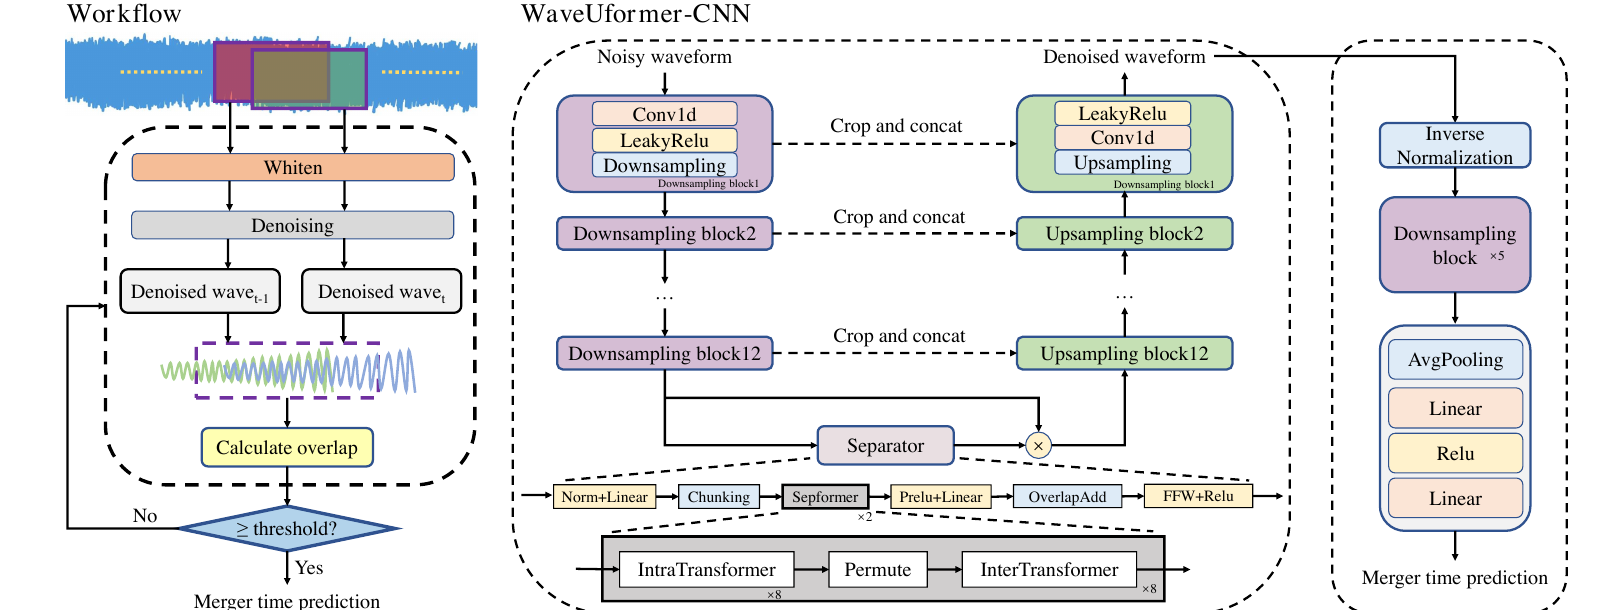
\includegraphics[width=0.98\textwidth]{figures/Xu2024_denoising_fig1_workflow.png}
\caption{长时旋近信号去噪与并合时刻预测的整体流程和 WaveUformer-CNN 架构。左侧展示滑动时间窗数据经白化和去噪后，通过相邻窗口去噪波形的重叠度判断是否出现可用信号，并在超过阈值后进入并合时刻预测；右侧展示用于去噪的 WaveUformer 结构与用于并合时刻预测的 CNN 后端。图据 Xu 等~\cite{xu2024denoising} 的 Figure 1 裁切引入。}
\label{fig:long_inspiral_denoising}
\end{figure}

\subsection{多信使预警的时间窗口需求}

大质量双黑洞并合的多信使观测对预警时间有较高要求。不同类型的电磁观测设施有不同的准备时间：X 射线望远镜的指向调整通常需要数小时；地面光学望远镜的目标规划可能需要提前一天以上；射电望远镜阵列的相关器配置则可能需要更长时间。因此，24 小时量级的并合时刻预测精度，是评估空间任务多信使预警能力的重要参考指标。

从旋近阶段的频率演化外推并合时刻，其精度取决于两个因素：去噪后信号的质量（重叠度越高，频率演化估计越准确）和外推时间窗口的长度（距并合越近，外推误差越小）。Xu 等人的工作表明，在并合前 10 天的旋近数据上，去噪后的重叠度足以支持 24 小时精度的并合时刻预测，这一结果为太极任务的多信使预警系统设计提供了关键的技术参数。

去噪框架在处理30天旋进信号时面临的核心技术挑战，值得从信号处理的角度进行深入分析。30天的旋进信号即便以较低采样率记录，也对应百万量级的数据点，远长于地面探测器常见的秒级紧致双星数据段。这一长度差异带来若干算法挑战：其一，信号频率在毫赫兹频段缓慢演化，跨越的时间尺度远长于常规时序网络的有效上下文；其二，信号幅度随并合临近显著增强，动态范围较大；其三，长时间跨度内探测器噪声的非平稳性、数据间隙和暂态噪声会累积影响信号连续性。Xu等的解决方案是将长时数据分割为若干较短片段，对每段独立去噪后再拼接，并在拼接处进行平滑处理以降低边界不连续性。这一分段策略的代价是可能损失跨段相关信息，因此分段长度、重叠比例和拼接策略需要随信号模型和噪声条件重新优化。

除并合时刻预测外，旋进阶段的高质量去噪还可支持实时引力波参数估计。传统贝叶斯参数估计通常在并合后数小时至数天才能完成；利用旋进阶段的去噪信号，则可以在并合发生前逐步积累参数信息：对新到来的旋进数据段运行SBI参数估计，并用贝叶斯更新逐步细化后验，有望在并合前给出质量、自旋和天空位置的初步约束。这一“实时在线参数估计”能力若能实现，将提升多信使观测的针对性：不仅知道“何时”可能发生并合，还能提前得到“在哪里”和“是什么类型”的粗略信息，从而更高效地分配望远镜资源。对于总质量约$10^6 M_\odot$量级的大质量双黑洞系统，旋进阶段可能持续数周，在线参数估计的精度可随数据积累逐步改善。这一能力的实现，要求去噪、参数估计与在线更新模块紧密协作，是未来实时空间引力波数据处理的重要目标。

\section{非稳态噪声下的鲁棒信号提取}

地面引力波探测器的噪声虽然复杂，但在短时间尺度上近似平稳，现有去噪方法已能较好处理。空间引力波探测器则面临更严峻的挑战：由于卫星在太空中运行，仪器噪声会出现多种形式的非稳态特性，这些特性在地面测试中难以完全预测和模拟。

Xu 等人~\cite{xu2024nonstationarty} 系统研究了三类可预见的非稳态噪声对信号提取的影响，并开发了相应的鲁棒深度学习模型：

\textbf{数据间隙}（Data Gaps）：由于例行维护或意外中断，探测器数据流中会出现缺失段。数据间隙破坏了信号的时域连续性，使基于连续时序的去噪方法失效。

\textbf{暂态噪声}（Glitches）：仪器或环境扰动产生的短时高幅度噪声脉冲，其统计特性与背景噪声截然不同，会在去噪输出中留下伪信号。

\textbf{时变噪声自相关}（Time-Varying Noise Auto-Correlations）：噪声的功率谱密度随时间缓慢变化，使基于固定噪声模型的去噪方法逐渐失效。

该工作开发的深度学习模型在理想无异常场景中性能与代表性基线模型相当，同时在面对上述三类非稳态噪声（及其混合情形）时表现出显著的适应性。这一鲁棒性来自训练数据的系统性设计：通过在训练集中引入各类非稳态噪声的模拟样本，使网络学习到对噪声类型变化的不变特征表示。

这一工作的意义超越了单一方法的改进。它强调了空间引力波数据分析中一个容易被理想化模拟低估的挑战：非稳态噪声并非罕见例外，而可能是长期在轨运行中需要持续处理的常见现象。面向实用的空间引力波数据分析管道，应将非稳态噪声鲁棒性作为早期设计要求之一，而不是在算法定型后再被动补充。

\begin{figure}[htbp]
\centering
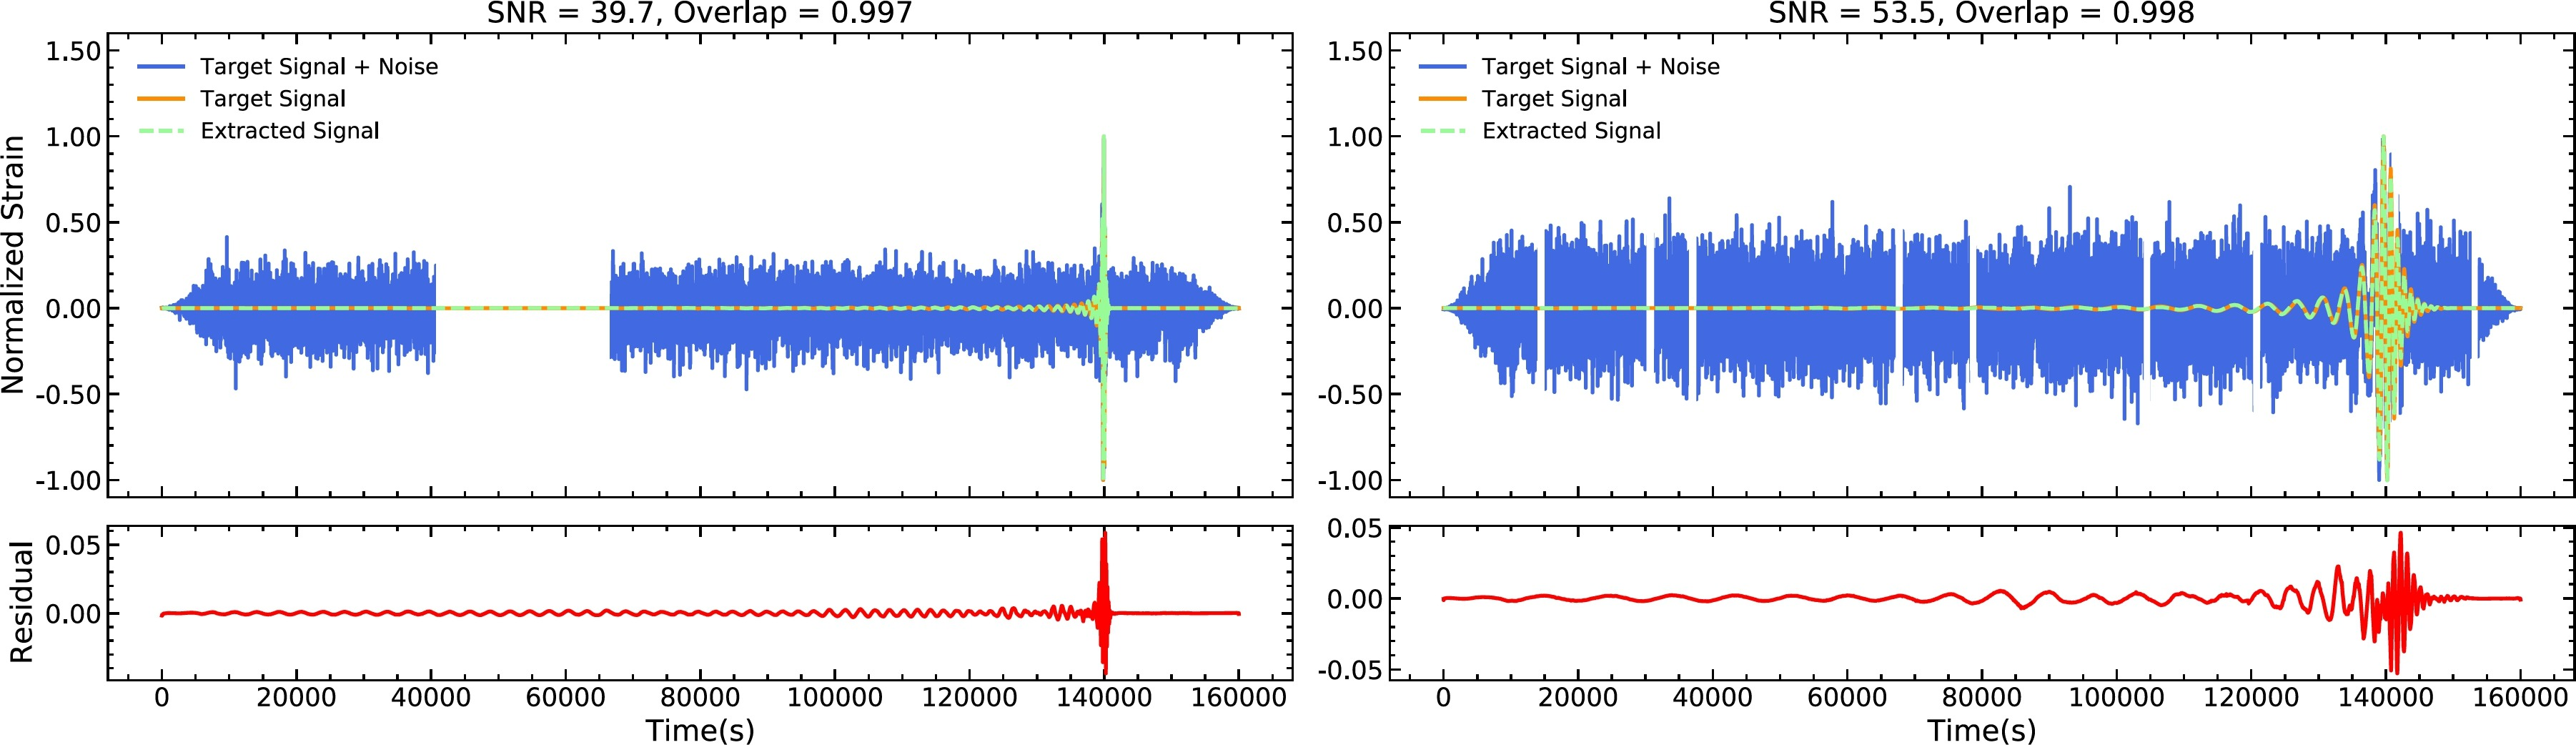
\includegraphics[width=0.98\textwidth]{figures/Xu2024_nonstationary_fig5.jpg}
\caption{深度学习模型在空间探测器非稳态噪声条件下的信号提取示例。蓝色曲线为含噪目标信号，橙色曲线为注入的目标信号，绿色虚线为模型提取信号，下方红色曲线为残差；图中两个测试样本分别给出较高信噪比条件下的重叠度结果，说明在数据异常和非稳态噪声存在时，鲁棒模型仍可恢复主要波形结构。图引自 Xu 等~\cite{xu2024nonstationarty} 的 Figure 5。}
\label{fig:nonstationary_noise}
\end{figure}

时变噪声自相关（time-varying noise auto-correlations）是三类非稳态噪声中技术上较难处理的一类，因为它不像数据间隙那样有清晰的时间边界，也不像glitch那样有明显的幅度异常，而是以渐进方式改变噪声统计特性。在探测器实际运行中，热环境变化、检验质量带电、太阳活动和激光链路状态变化等因素都可能导致噪声功率谱密度在小时至天的时间尺度上缓慢漂移，使基于固定噪声模型的去噪方法逐渐失配。处理这一问题的一类思路是“滑动窗口PSD估计”：在连续数据上实时估计噪声PSD，并据此更新白化滤波器或网络归一化参数。自适应白化的引入，使去噪网络不必完全依赖训练数据中的噪声多样性来应对PSD漂移，而是通过估计-更新的闭环机制适应噪声变化。其效果需要在不同漂移幅度、数据间隙模式和在轨噪声模型下系统评估，但这一方向体现了“物理感知去噪”与自适应信号处理的结合。

\subsection{鲁棒去噪的训练数据设计原则}

深度学习去噪模型的鲁棒性来源于两个相互强化的机制：训练数据的系统性设计和网络架构的适应性。训练数据层面，Xu等在训练集中引入三类非稳态噪声的模拟样本，比例约为30\%，其余70\%为理想高斯噪声样本，这种混合训练策略迫使网络学习对噪声类型变化不敏感的信号特征——即引力波信号本身的物理特征（啁啾、时频演化、极化方式），而非特定噪声背景下的统计关联。这一思路与计算机视觉中的数据增强（data augmentation）有深刻的类比：通过在训练时引入旋转、缩放、亮度变化等变换，强迫图像识别网络学习对几何变换不变的高层特征；引力波去噪中，“噪声类型变换”相当于一种特殊的数据增强，强迫网络学习对噪声统计特性不变的信号特征。

网络架构层面，掩码注意力（masked attention）机制是处理数据间隙的关键设计。当数据流中存在缺失段时，自注意力矩阵 $\mathrm{softmax}(QK^T/\sqrt{d_k})V$ 中对应间隙位置的查询键值对被屏蔽（设为负无穷），使得网络在计算当前时间步的表示时忽略缺失数据的影响。间隙内部的输出通过对间隙前后有效数据的注意力权重进行内插得到，内插质量取决于间隙长度和前后信号的特征相似度：短间隙（$<10$秒）通常能高质量内插，长间隙（$>100$秒）则不确定度大，需要在输出中相应标记可信度较低的区域。

暂态噪声（glitch）的处理是鲁棒去噪中另一个核心技术难点，其难度来自glitch与引力波信号在时频域的相似性。部分glitch类型在Q变换时频图中可能表现出与双黑洞并合信号相近的局部结构，导致去噪网络将高振幅glitch错误地“保留”甚至“增强”。Xu等的鲁棒模型通过在训练数据中混入纯glitch样本（不含引力波信号），并将其标注为期望输出接近零，促使网络学习识别并抑制glitch特征。该策略可通过glitch抑制率和注入信号重叠度联合评估；在其模拟设置中，模型对多类glitch表现出较好的能量抑制能力，同时保持了较高的信号重叠度。需要注意的是，“glitch抑制”与“信号保真”之间存在真实权衡：过度强调glitch抑制可能导致网络在glitch附近过度平滑，损失真实信号细节；过度强调信号保真则可能提高虚假信号输出风险。自适应损失权重为这一权衡提供了一种工程化方案，但最优权重仍需随任务噪声模型和科学目标重新标定。

\subsection{深度去噪与参数估计精度的定量关联}

理解去噪质量如何影响参数估计精度，是评估去噪方法科学价值的关键。从理论角度，重叠度 $\mathcal{O}(\hat{h}, h)$ 与匹配滤波SNR存在直接关系；若将去噪后的信号 $\hat{h}$ 作为下游参数估计的输入，重叠度不足可能表现为SNR损失、相位偏差或后验宽度变化。对于 $\mathcal{O}=0.97$，对应的失配约为几个百分点；对于 $\mathcal{O}=0.95$，失配已达到需要谨慎评估的水平。能否接受这一误差取决于科学目标：快速预警可容忍较粗略的估计，而精密测量则需要更严格的相位和幅度保真度检验。

在实际应用中，去噪的价值体现在两个场景：其一是对已有信号的“增强”——在低SNR事件上，去噪可能改善下游参数估计的稳定性，特别是对天空位置等多模态后验有潜在帮助；其二是对全局拟合的“预处理”——在空间探测器的信号叠加场景中，先对强信号去噪再减除，有望降低减除后残差中的信号污染，提高下一轮弱信号分析的精度。Xu等的旋进去噪框架特别针对第二个场景设计；在其模拟设置中，对MBHB旋进信号的高质量去噪可降低残差信号泄漏，并改善后续EMRI搜索条件。这说明去噪与全局拟合之间存在系统性耦合，但具体增益仍需在完整管道和更真实噪声模型下验证。

\subsection{去噪方法的计算效率与实时性}

空间引力波探测器的主科学数据采样率通常远低于地面探测器；若按1 Hz单通道采样估算，每天约有86,400个采样点，但实际分析还需处理多个 TDI 通道、标定信息和数据质量信息。其数据体量本身未必大于地面探测器，真正困难在于信号持续时间极长（MBHB旋进可达数月）且多源叠加严重。在实时处理要求下，深度去噪网络的前向传播速度需要满足两个约束：（1）处理速度必须快于数据产生速度（实时性约束）；（2）对于并合时刻预测应用，必须在并合前数天完成预测（低延迟约束）。

对于WaveFormer类的Transformer架构，处理一天数据在GPU上的推断时间通常可远短于数据产生时间，因而实时性约束在计算层面并非主要瓶颈。低延迟约束则更为关键：若要求在并合前数天给出24小时量级的并合时刻预测，需要在数据积累后尽快完成去噪、频率提取和外推分析。现有模拟实验表明，深度去噪方法在推断速度上具有满足低延迟预警需求的潜力；但真实管道还必须计入数据质量标记、TDI处理、异常段处理和结果交叉验证的开销，因此仍需端到端系统测试。

在实践中，非稳态噪声鲁棒性的测试必须在接近真实任务条件的数据上进行，这对太空任务的去噪算法开发提出了特殊挑战：真实的太空噪声数据在发射前不可获得，只能依赖地面测试、技术验证任务和理论模型来模拟。这一“数据可用性悖论”意味着：算法必须在基于预测噪声特性的模拟数据上训练，同时又要准备面对实际在轨测量才会揭示的噪声形态。解决这一悖论的一种策略是设计具有广泛适应性的模型，而非针对单一噪声特征优化的专用模型。Xu等的鲁棒去噪方法通过系统引入多种非稳态噪声类型的混合训练数据，是这一思路的一个实现。但仅凭地面预测模型仍难以覆盖全部在轨噪声形态，因此未来需要结合技术验证卫星和主任务早期标定数据持续更新模型，形成“发射前预训练+在轨标定微调”的开发策略。这一策略同样适用于信号检测、参数估计等数据处理链路，是空间引力波数据处理系统工程设计的重要原则。

\section{本章小结}

\begin{figure}[htbp]
\centering
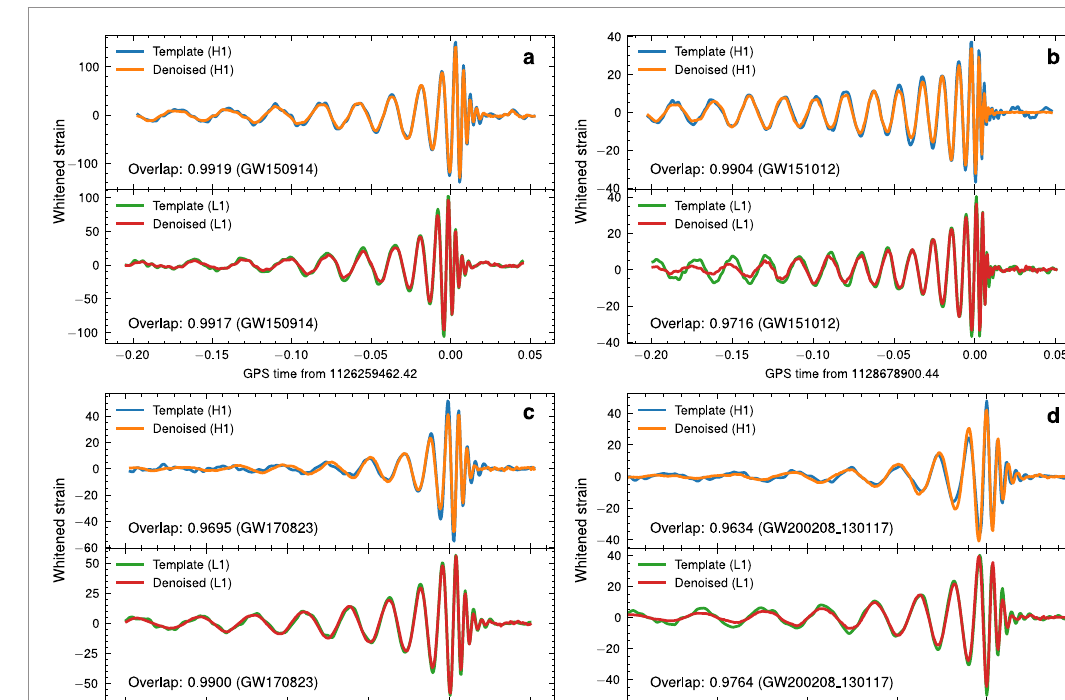
\includegraphics[width=0.92\textwidth]{figures/WaveFormer_Figure5_denoising_events.png}
\caption{WaveFormer 在真实 LIGO 观测事件上的去噪结果示例。图中以 GW150914 为例展示了去噪前后的白化应变、振幅谱密度以及 H1/L1 两台探测器中去噪输出与最优模板的相位对齐情况；原文 Figure 5 还比较了 GW151012、GW170823 和 GW200208\_130117 等事件，说明 WaveFormer 在低网络信噪比或较高啁啾质量情形下仍能恢复主要相位结构和振幅峰值。图引自 Wang 等~\cite{wang2024waveformer} 的 Figure 5。}
\label{fig:denoising_example}
\end{figure}

图~\ref{fig:denoising_example} 体现了深度去噪方法科学价值的关键：评价对象不是视觉上更“干净”的波形，而是去噪输出能否在相位、振幅和频谱结构上与物理模板保持一致。对于 GW150914，WaveFormer 的输出在两台探测器中均与模板具有很高的重叠度，尤其能较好恢复并合和衰荡附近的相位结构；对低网络信噪比事件和较高啁啾质量事件，论文中的进一步比较也显示了网络对不同观测条件的适应性。需要强调的是，这类结果仍应被理解为经过特定训练分布和后处理流程校准后的经验性能，不能替代完整的事件显著性评估和参数估计误差分析。

\begin{table}[htbp]
\centering
\caption{引力波去噪方法性能对比}
\label{tab:denoising_methods}
\small
\begin{tabular}{lcccc}
\hline
\textbf{方法} & \textbf{架构} & \textbf{重叠度 $\mathcal{O}$} & \textbf{推断时间} & \textbf{主要优势} \\
\hline
维纳滤波 & 线性滤波器 & 0.85--0.92 & $<1$ ms & 无需训练，线性基准 \\
小波阈值 & 多尺度分解 & 0.88--0.93 & $<1$ ms & 非平稳适应性 \\
U-Net CNN & 编解码器 & 0.93--0.96 & $\sim 5$ ms & 多尺度特征提取 \\
WaveFormer & Transformer & 0.96--0.98 & $\sim 10$ ms & 全局时频依赖 \\
WaveFormer（鲁棒） & Transformer+掩码注意力 & 0.93--0.97 & $\sim 15$ ms & 非稳态噪声鲁棒 \\
\hline
\end{tabular}
\end{table}

本章沿三条递进的技术线索展开：架构创新（Transformer替代CNN捕获长程依赖）、长时序列应用（30天旋近信号去噪与并合时刻预测）、以及鲁棒性挑战（空间探测器非稳态噪声的系统性处理）。

去噪技术与全书其他方法论的关联，构成了一个有机的技术生态系统。MF-CNN（第5章）利用物理先验在检测阶段增强对glitch的鉴别能力，其感知层设计可以理解为一种“检测时去噪”；WaveFormer（本章）则是“检测前去噪”——在数据进入匹配滤波或深度学习检测器之前，先行提升数据质量。SBI（第6章）的参数估计精度直接受输入数据质量影响，高质量且经过校准的去噪输出有助于使SBI的后验分布更稳定。Evo-MCTS（第8章）发现的PT-4算法中包含了信号平滑步骤（Savitzky-Golay滤波），可理解为轻量级的“在线去噪”操作。物理-数据融合（第9章）在去噪领域的体现是用引力波信号的物理模型约束去噪网络的输出，使去噪结果不仅噪声更低，还更符合物理预期。

这些关联表明，去噪不是孤立的数据处理步骤，而是整个引力波人工智能分析生态系统的重要组成部分。架构创新方面，WaveFormer将Transformer的自注意力机制引入引力波去噪，通过全局依赖建模缓解了CNN局部感受野的限制，在若干测试设置下优于基于CNN的方法。长时序列应用方面，针对空间探测器大质量双黑洞并合的多信使预警需求，专为30天连续旋近信号设计的深度神经网络去噪框架，在SNR 10--50的模拟条件下实现并合时刻预测误差通常在24小时以内，将引力波去噪从数据质量提升连接到多信使天文学的实际观测需求。鲁棒性挑战方面，针对空间探测器三类可预见非稳态噪声（数据间隙、暂态噪声、时变噪声自相关）的系统性研究，提示非稳态噪声应被视为空间任务运行中的常见挑战，面向实用的数据分析管道应在早期设计阶段纳入鲁棒性要求。这三条线索共同指向一个核心认识：引力波去噪不是单纯的信号处理问题，而是与多信使天文学科学目标直接挂钩的关键技术。


%% ================================================================
%% 第四部：综合创新与融合
%% ================================================================
\foottheme{}
\footimage{figures/faraday.jpg}
\foottext{物理驱动与数据驱动的融合，不是两种方法的简单叠加，而是在更高层次上的方法论统一。\hfill —— 本书第四部}
\pagestyle{mystyle}

\part{物理约束与智能方法融合}

\renewcommand{\parttitle}{物理约束与智能方法融合}

\chapter{智能启发式搜索与算法优化}

引力波数据分析的核心挑战之一，是在一个极其庞大的算法设计空间中寻找高性能的信号处理策略。匹配滤波依赖预先构建的波形模板库，其最优性以已知信号形态和高斯平稳噪声假设为前提；深度神经网络虽然弱化了显式模板依赖，却通常增加了可解释性和校准验证的难度。本章探讨第三条路线：将大语言模型（LLM）的领域知识生成能力与结构化进化搜索相结合，实现对引力波检测算法的自动发现。这一路线的核心优势在于，所发现的算法由可检视的代码组成，其决策逻辑更容易接受物理学家的审查和验证。

\section{算法设计作为搜索问题}

引力波信号处理管道通常由若干功能模块串联构成：数据白化、时频变换、跨探测器相干统计量构造、阈值判决等。每个模块的具体实现——选用何种滤波器、如何组合多探测器信息、采用何种统计量——都对应一个离散的设计选择。将所有可能的模块组合视为一个搜索空间，引力波检测算法的设计问题便转化为：在该空间中找到使某一性能指标（如敏感距离 AUC）最大化的程序~\cite{schafer2023mlgwsc1}。

这一视角揭示了传统方法在大规模组合搜索中的局限。手工设计依赖专家经验，容易受既有知识结构和探索能力约束；网格搜索在组合爆炸面前迅速失效；遗传编程虽能自动搜索，却若缺乏领域知识引导，往往生成大量物理上无意义的候选。大语言模型的出现为这一问题提供了新的可能~\cite{romera2024funsearch}：LLM 在预训练阶段接触过大量科学和工程文本，能够生成语法正确且部分物理上合理的候选算法，从而将搜索空间从“任意可能的程序”压缩到“更可能有物理意义的程序”这一较小子集。

\subsection{AutoML 与神经架构搜索的启示}

在算法设计自动化领域，自动机器学习（AutoML）和神经架构搜索（NAS）是两条已有成熟实践的技术路线。AutoML 通过自动化超参数搜索——包括贝叶斯优化、进化算法和强化学习等策略——大幅减少了模型调优所需的人工干预。在图像分类基准任务上，NAS 自动发现的网络架构（如 DARTS 和 EfficientNet 系列）曾在 ImageNet 等基准上取得有竞争力的结果，说明算法设计空间的系统性搜索能够发现人类专家难以直接想到的高效结构。

然而，将这些成功经验直接移植到科学计算领域时，面临一系列本质性的新挑战。首先，评估函数的计算代价远高于图像分类。引力波检测性能的标准指标——误报率下的敏感距离曲线（FAR-sensitive distance curve）——需要在大量真实或模拟噪声数据上统计计算，单次评估耗时30至60秒（在 GPU 加速条件下），是图像分类准确率评估的数百倍。其次，设计空间包含领域特定的物理约束，这些约束对通用搜索算法并不透明：白化操作必须正确估计并消除噪声的功率谱密度，跨探测器相干统计量的构造必须尊重引力波在两个探测器间的时间延迟关系（最大10毫秒），匹配滤波的实现必须处理非平稳噪声的短时变化。通用 NAS 方法在这样的约束空间中搜索，极易生成物理上无意义的候选，浪费宝贵的评估配额。

\subsection{引力波管道的模块化形式化描述}

为了将算法设计问题纳入严格的数学框架，我们首先建立引力波信号处理管道的模块化形式化描述。一个典型的引力波检测管道可以抽象为一系列函数的复合：
\begin{equation}
f_{\text{detect}} = f_n \circ f_{n-1} \circ \cdots \circ f_2 \circ f_1,
\end{equation}
其中每个 $f_i$ 对应一个具体的处理步骤。以 MLGWSC-1 标准管道为例，$f_1$ 可能是白化操作，$f_2$ 是时频变换（可以是 Q 变换、短时傅里叶变换 STFT 或连续小波变换 CWT），$f_3$ 是跨探测器相干统计量的构造，$f_4$ 是对统计量的平滑与阈值判决。每个步骤不仅有若干可选的实现方式，还有多个可调的连续参数——白化的基线长度、时频变换的窗口宽度和重叠率、相干统计量的时延搜索范围等。

这一形式化描述揭示了搜索空间的组合爆炸性质。若每个步骤有 $k$ 种可选实现，各有 $m$ 个离散可调参数，则整个管道的搜索空间大小约为 $O(k^n \cdot m^{n \cdot p})$，其中 $p$ 是每步参数数量。即便取保守估计（$n=5$，$k=4$，$m=3$，$p=3$），搜索空间大小已超过 $10^{10}$，远超任何穷举策略的可行范围。更重要的是，这一搜索空间中绝大多数点对应物理上无意义的管道——例如，跳过白化步骤直接对原始数据应用匹配滤波会使非平稳噪声干扰信号检测；逆序执行步骤（先阈值判决后时频变换）在信号处理上没有意义。因此，高效搜索的关键在于如何利用领域知识约束搜索空间，而非盲目枚举。

\subsection{程序搜索的数学框架}

将管道搜索问题形式化为黑箱优化，可以写成：
\begin{equation}
\theta^* = \arg\max_{\theta \in \Theta} \mathcal{F}(\text{code}(\theta)),
\end{equation}
其中 $\theta$ 是描述管道结构（模块选择和组合方式）的参数向量，$\text{code}(\theta)$ 是由 $\theta$ 描述的可执行程序，$\mathcal{F}$ 是评估函数（在 MLGWSC-1 上即为敏感距离 AUC），$\Theta$ 是所有物理上合理的参数配置的集合。

这一框架与标准超参数优化的本质区别在于：$\theta$ 是离散的程序结构参数，而非连续的实数向量。这使得基于梯度的优化方法（如 Adam、SGD）无法直接应用——因为 $\text{code}(\theta)$ 关于 $\theta$ 的梯度在离散空间中无法定义。即便将结构参数松弛到连续空间（类似 DARTS 的做法），引力波评估函数 $\mathcal{F}$ 的高计算代价也使得梯度估计（需要对每个参数进行有限差分近似）在实践中不可行。

这一分析确立了为何需要无梯度的黑箱优化策略——进化算法和贝叶斯优化是两类自然的候选。但如下文所展示的，在科学计算领域，这两类通用策略还需要与领域知识深度结合，才能在有限的评估预算内找到高性能的解。

从更宏观的视角来看，将算法设计问题视为搜索问题这一框架转换，本身就具有重要的认识论意义。传统的算法设计隐含着一种以人类专家为中心的知识创造模式：算法的每一步改进都是研究者通过分析现有方法的局限、结合物理直觉、设计新的解决方案，再通过实验验证的结果。这一过程的效率上限由人类研究者的认知带宽决定，且存在系统性的认知偏见——研究者倾向于探索自己熟悉的算法结构空间（如CNN架构或匹配滤波变体），而难以主动探索与已有知识结构差异较大的“陌生”算法组合。将算法设计形式化为黑箱优化问题，则将人类专家从“主动设计者”转变为“问题定义者”和“评估者”——专家负责定义性能指标（MLGWSC-1敏感距离）、注入领域约束（物理约束提示词）、以及审查搜索结果的物理合理性，而算法空间的探索则由LLM驱动的自动搜索完成。这一角色转变不是对专家知识的替代，而是对专家时间和注意力的重新分配：从在算法细节上反复试错，到在高层次的问题定义和物理约束上投入更多精力。在引力波信号处理这一涉及深厚物理知识的领域，这种人机协作模式将人类专家的物理洞察、约束识别与结果验证能力，同人工智能系统的高并发搜索和系统性探索能力结合起来，代表了引力波人工智能研究方法论的重要演进方向。

\section{LLM驱动的自动启发式设计}

将 LLM 与进化搜索结合用于自动算法发现，近年来形成了一条清晰的方法演进脉络。

\textbf{FunSearch}~\cite{romera2024funsearch} 是这一范式的奠基性工作。Google DeepMind 于 2023 年在 \textit{Nature} 上报告，FunSearch 将预训练 LLM 与自动评估器配对，在程序空间中进行进化搜索。LLM 负责生成多样化的候选程序，评估器过滤错误输出并防止幻觉传播，进化机制在高分程序之间进行重组。FunSearch 在极值组合数学的 cap set 问题上发现了改进既有构造的新方案，说明 LLM 驱动的程序搜索有可能在严格评估器约束下产生具有科学价值的候选结果。

\textbf{EoH}（Evolution of Heuristics）~\cite{liu2024eoh} 将这一思路推进到启发式算法设计领域。EoH 的关键创新在于引入双层进化：不仅进化可执行代码，还同时进化描述启发式设计思路的自然语言（“thought”）。LLM 将思路翻译为代码，进化操作同时作用于两个层次。在在线装箱、旅行商等组合优化基准上，EoH 超越了人工设计的启发式算法。

\textbf{ReEvo}（Reflective Evolution）~\cite{ye2024reevo} 进一步引入“反思”机制。ReEvo 让 LLM 分析高分与低分候选之间的差异，生成“语言梯度”（verbal gradient）——一种以自然语言表达的改进方向——从而为进化搜索提供更有针对性的引导。ReEvo 在 TSP（旅行商问题）、CVRP（有容量约束的车辆路径问题）等多个 NP-hard 问题上取得了较强的 LLM-based AHD 基准结果。

上述方法均针对组合优化问题，其候选解为离散决策序列，评估函数定义明确。引力波信号处理问题则呈现出本质不同的挑战：候选解是连续参数优化的信号处理管道，需要满足物理约束，且评估指标（敏感距离 AUC）的计算涉及真实噪声数据，代价较高。这些差异促使了 Evo-MCTS 框架的提出。

从 FunSearch 到 EoH 到 ReEvo 再到 Evo-MCTS 的演进轨迹，体现了 LLM 驱动自动算法发现方法论的快速发展。这一演进可以从三个维度来理解：第一，知识注入的深化——FunSearch 使用通用领域知识，EoH 引入问题特定的设计思路，ReEvo 加入比较性学习（分析高分vs低分的差异），Evo-MCTS 引入深度领域专业知识（物理约束、信号处理原则）；第二，搜索结构的完善——从简单进化库（FunSearch）到思路-代码双层结构（EoH），再到MCTS树结构的多尺度探索（Evo-MCTS），搜索空间的导航越来越有组织；第三，应用场景的复杂化——从纯数学问题（cap set）到离散优化（TSP、CVRP）再到物理科学计算（引力波检测），候选解的约束越来越多，评估函数越来越复杂。这一演进表明，LLM 驱动的自动算法发现正在从相对清晰的基准问题向更复杂的实际问题推进。Evo-MCTS 在引力波这一高度专业化的科学计算问题上的表现，是这一推进过程中的一个案例，也提示类似框架未来有必要在更广泛的科学计算领域接受系统检验。

\subsection{FunSearch 的工作流程细节}

FunSearch 的核心架构由三个相互协作的组件构成。评估器（evaluator）对每个候选程序运行沙箱测试，返回性能分数，并过滤语法错误和运行时错误——这一过滤机制至关重要，因为 LLM 生成的代码有相当比例存在语法错误或逻辑缺陷，若不过滤则会污染进化库。进化库（program database）维护当前高分程序的集合，按性能和多样性双重标准排序：仅保留高分程序会导致多样性丧失，而仅保留多样程序则会浪费评估配额在低质量候选上。LLM 在看到库中的高分程序和相关问题描述后，生成改进版本；这一“看到优良候选后改进”的机制类似于人类专家在阅读前人工作后提出改进方案的认知过程。

在 cap set 问题上，FunSearch 找到了 $n=8$ 时大小为 $512$ 的 cap set（此前已知构造为 $509$），是由 LLM 驱动的程序搜索发现数学新构造的代表性案例。这一结果的意义不仅在于数值上的改进，更在于说明 LLM 驱动的搜索有可能在严格评估器约束下发现人类专家尚未系统探索的结构——这为将类似方法应用于科学计算中的算法发现提供了有力先例。

\subsection{EoH 的双层进化机制}

EoH 的核心创新在于将启发式算法的“设计意图”与“具体实现”解耦，并在两个层次上同时进行进化。自然语言描述（“thought”）编码了启发式算法的设计意图，例如“优先选择约束最强的变量”或“在局部搜索中优先探索高密度区域”。LLM 将这些自然语言描述翻译为可执行的 Python 代码，形成候选启发式算法。

进化算子同时作用于 thought 和 code 两个层面。思路层面的交叉操作将两个算法的设计意图合并（例如“结合 A 的约束优先策略和 B 的密度感知策略”），由 LLM 翻译成新的代码实现；代码层面的变异操作直接修改代码的局部结构，保留整体设计意图。这种双层进化使得搜索能够在高层语义空间（设计思路）和低层实现空间（代码细节）之间协同探索，避免了单纯代码进化中常见的“语义漂移”问题——即代码在形式上发生变化但实际功能退化。

在在线装箱（online bin packing）问题上，EoH 生成的启发式在标准测试集上比人工设计的 best-fit-decreasing 算法好约 3\%。这一提升看似不大，但考虑到 best-fit-decreasing 是经过长期优化的经典算法，EoH 在有限搜索预算内取得可比并略优的结果具有重要的方法论意义。

\subsection{ReEvo 的语言梯度机制}

ReEvo 的核心创新是“语言梯度”（verbal gradient）概念。在标准梯度下降中，梯度向量指示了参数空间中性能提升最快的方向；在离散的程序空间中，梯度无法直接定义，但 ReEvo 通过 LLM 的语言理解能力构造了一种类似的引导信号。

具体地，对高分候选 $p^+$ 和低分候选 $p^-$，ReEvo 提示 LLM 分析“为什么 $p^+$ 比 $p^-$ 更好？”。LLM 生成的文本描述指出两者的关键差异——例如“$p^+$ 在局部搜索阶段使用了更细粒度的邻域结构，而 $p^-$ 的邻域过于粗糙导致错过了局部最优”——这一描述作为下一轮改进的方向，引导 LLM 生成融合 $p^+$ 优点并修正 $p^-$ 缺陷的新候选。

这种机制类似于梯度下降，但作用在离散的程序空间上，且“梯度”以人类可读的自然语言形式表达，具有内在的可解释性。在 TSP 上，ReEvo 生成的构造启发式比 LKH3 竞争性算法只差约 1\%（此前 LLM 方法与 LKH3 的差距约为 10\%--20\%），显示了语言梯度机制在缩小 LLM 方法与专业求解器差距方面的有效性。

\subsection{从组合优化到科学计算的挑战}

上述三种方法在组合优化领域取得了令人印象深刻的结果，但将其直接应用于引力波检测算法发现时，面临若干本质性的新挑战。

第一，评估函数的统计性质。组合优化问题的评估通常是确定性的：给定输入，解的质量可以精确计算（如 TSP 的路径总长度）。引力波检测的评估涉及统计量——误报率（FAR）和敏感距离是在大量数据上的统计量，单次评估含有不可忽略的随机噪声。这意味着同一算法在不同评估运行中可能得到不同的分数，进化选择机制需要能够处理这种评估噪声，避免将随机高分误认为真正的性能提升。

第二，候选解的混合离散-连续性质。组合优化的解通常是纯离散的决策序列（如 TSP 的城市访问顺序），而引力波管道包含大量连续参数（白化滤波器的截止频率、时频变换的窗口宽度、相干统计量的阈值等）。这些连续参数需要在离散的程序结构搜索之外进行额外的数值优化，形成双层优化问题。

第三，物理约束的隐式性。引力波管道的物理约束（如白化的必要性、相干统计量的时延范围）对通用 LLM 并不透明，需要通过精心设计的提示词将这些约束显式传达给 LLM。这些差异使得通用框架不能直接应用，需要专门适配，这正是 Evo-MCTS 框架设计的出发点。

\section{Evo-MCTS与可解释算法发现}

\textbf{Evo-MCTS}（Evolutionary Monte Carlo Tree Search）~\cite{wang2025evomcts} 是专为科学计算中的算法发现设计的框架，以引力波检测为核心案例研究。其核心思想是将 LLM 的领域知识生成能力、蒙特卡洛树搜索（MCTS）的结构化探索策略，以及进化计算的种群多样性维护机制三者有机整合。

\begin{figure}[htbp]
\centering
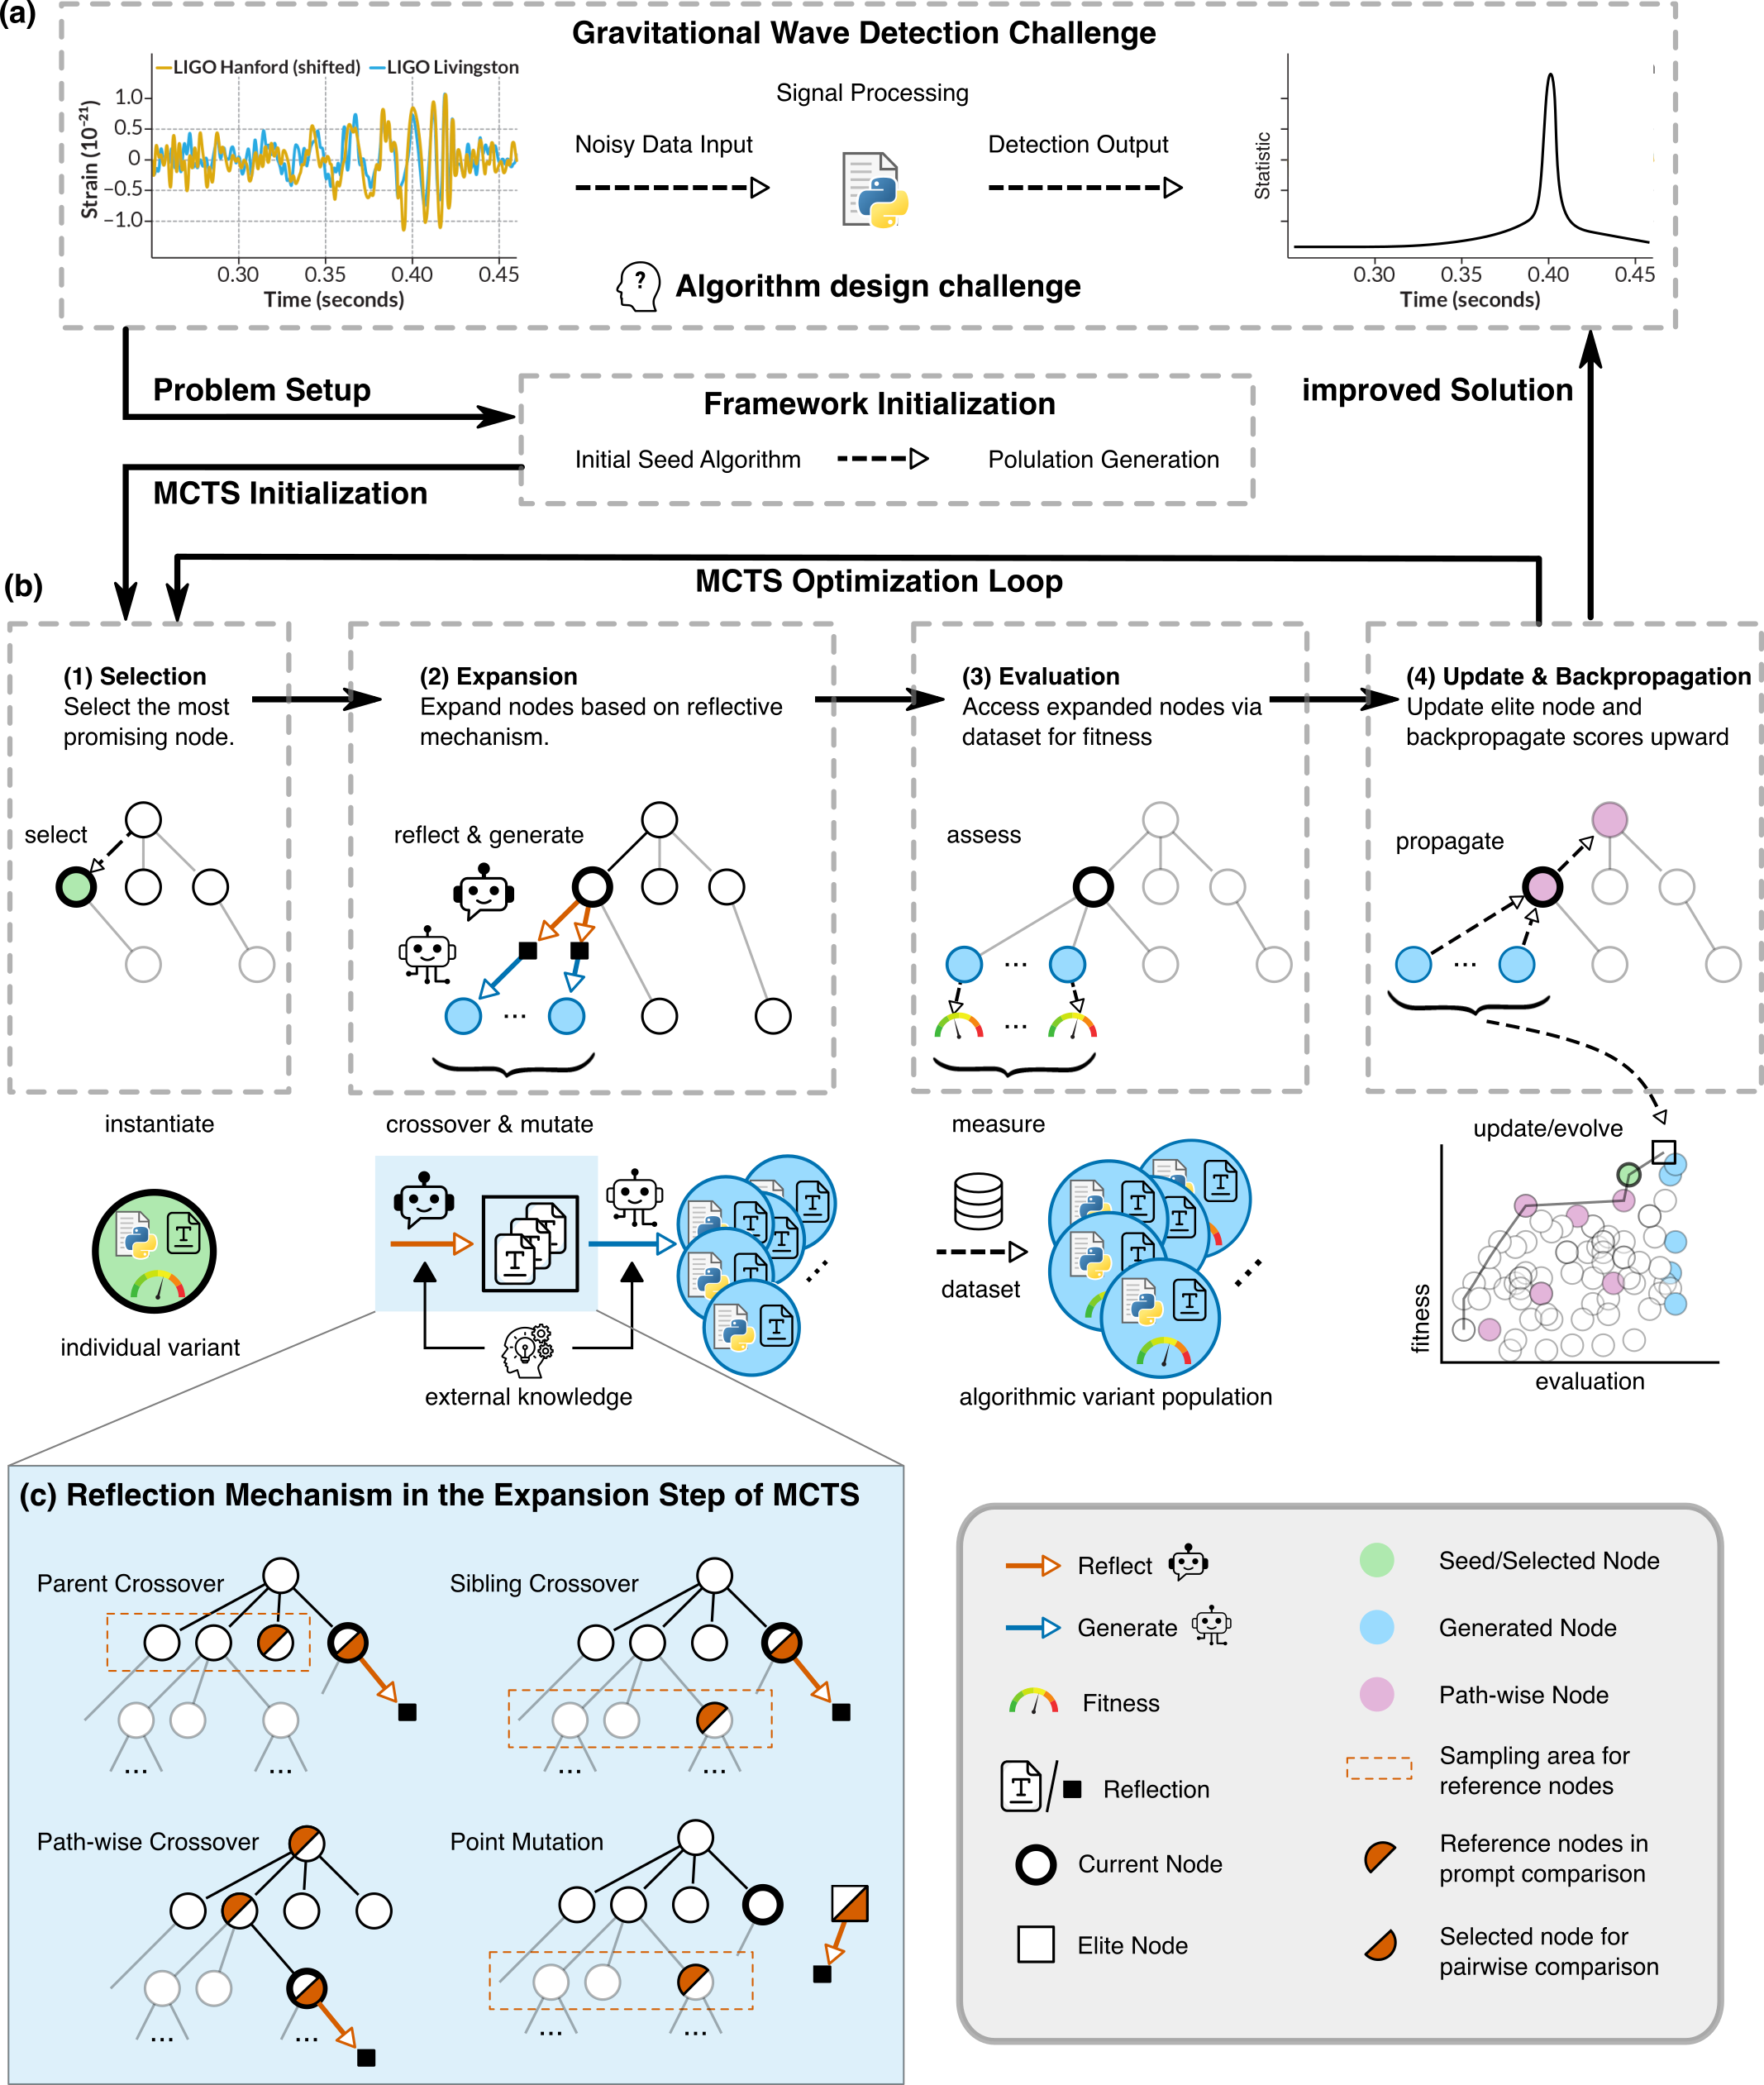
\includegraphics[height=0.72\textheight,keepaspectratio]{figures/EvoMCTS_fig1_framework.png}
\caption{Evo-MCTS 框架总体流程。框架以候选引力波检测程序为搜索对象，利用 LLM 生成和反思候选代码，以 MCTS 树组织探索历史，并通过父节点交叉、兄弟节点交叉、路径级交叉和点突变等操作产生新算法；每个候选解通过 MLGWSC-1 真实噪声基准上的适应度评估获得反馈。图引自 Wang 和 Zeng~\cite{wang2025evomcts} 的 Figure 1。}
\label{fig:evomcts_framework}
\end{figure}

\subsection{框架设计}

Evo-MCTS 包含三项相互增强的核心创新：

\textbf{反射式代码合成}（Reflective Code Synthesis）。LLM 在生成候选算法时，不仅利用通用编程知识，还通过精心设计的提示词（prompt）注入引力波信号处理的领域知识——包括白化的物理意义、跨探测器相干统计量的构造原理、时频分析方法的适用场景等。每次生成后，LLM 还对自身输出进行反思，识别潜在的物理不一致性并迭代修正。消融实验表明，领域知识集成将平均适应度从 1244.50 Mpc 提升至 2670.37 Mpc，提升幅度达 115\%。

\textbf{多尺度进化操作}（Multi-Scale Evolutionary Operations）。Evo-MCTS 在 MCTS 树结构上定义了四种进化操作，作用于结构化代码表示：
\begin{itemize}
  \item \textit{父节点交叉}（Parent Crossover）：重组当前节点与其父节点的算法组件；
  \item \textit{兄弟节点交叉}（Sibling Crossover）：在同层节点间交换功能模块；
  \item \textit{路径级交叉}（Path-wise Crossover）：沿树路径提取并重组多代算法的优秀片段；
  \item \textit{点突变}（Point Mutation）：对单一功能模块进行局部修改。
\end{itemize}
这些操作通过 MCTS 树遍历实现语义感知的算法变换，使搜索能够在保持物理合理性的同时探索多样化的算法结构。

\textbf{可解释算法路径}（Interpretable Algorithm Pathways）。MCTS 树结构自然记录了算法发现的完整演化轨迹。每个节点对应一个具体的算法实现，节点间的父子关系反映了算法改进的逻辑链条。这使得研究者能够事后追溯：哪些技术创新在哪个阶段被引入，各创新对性能的贡献如何量化。这一特性在深度神经网络方法中是缺失的。

\subsection{提示词设计与领域知识注入}

Evo-MCTS 的提示词设计是框架成功的关键工程要素之一。每次 LLM 调用的提示词模板包含五个主要部分，共约 2000--3000 个 token。

第一部分是任务描述，明确说明目标任务（MLGWSC-1 Dataset 4 上的引力波检测）、评估规则（敏感距离 AUC 的计算方式）和代码接口规范（输入输出格式、允许使用的库）。这一部分确保 LLM 生成的代码能够被评估器正确执行，避免接口不匹配导致的无效评估。

第二部分是物理约束说明，包括：引力波信号的基本特征（啁啾结构、时频演化、双探测器时延）；探测器噪声的统计特性（非平稳、非高斯、存在线谱噪声）；白化操作的必要性和正确实现方式；跨探测器相干统计量的物理意义和构造原则。这一部分将引力波物理学的核心知识以 LLM 可理解的自然语言形式传达，是领域知识集成的核心载体。

第三部分是当前高分算法代码，作为 LLM 改进的起点。提供具体的代码而非抽象描述，使 LLM 能够在已有成果的基础上进行有针对性的改进，而非从零开始生成。这一设计体现了“站在巨人肩膀上”的搜索策略。

第四部分是性能反馈，包括当前算法在测试集上的敏感距离数值、与基线的对比、以及通过分析识别出的性能瓶颈（例如“在低信噪比区间的检测率偏低”或“对进动信号的适应性不足”）。这一反馈使 LLM 能够有针对性地改进算法的薄弱环节。

第五部分是改进方向建议，基于领域知识提供具体的改进思路（例如“考虑使用更短的白化基线以适应噪声的短时非平稳性”或“尝试引入连续小波变换以捕获信号的时频局部特征”）。这些建议不是强制约束，而是引导 LLM 在物理上有意义的方向上探索。

\subsection{UCB 在 MCTS 中的适配}

蒙特卡洛树搜索（MCTS）的核心是上置信界（UCB）策略，用于平衡探索（exploration）和利用（exploitation）之间的权衡。标准 MCTS 使用 UCT（Upper Confidence Bound for Trees）公式：
\begin{equation}
\text{UCT}(v) = Q(v) + c \sqrt{\frac{\ln N(p(v))}{N(v)}},
\end{equation}
其中 $Q(v)$ 是节点 $v$ 的平均奖励（对应该节点算法的平均敏感距离），$N(v)$ 是节点 $v$ 被访问的次数，$N(p(v))$ 是其父节点的访问次数，$c$ 是控制探索-利用权衡的超参数。

在 Evo-MCTS 中，节点奖励是该节点对应算法在 MLGWSC-1 测试集上的敏感距离。UCT 公式的第一项鼓励选择历史表现好的节点（利用），第二项鼓励选择访问次数少的节点（探索）。参数 $c$ 的选择对搜索效率有重要影响：$c$ 过大会导致过度探索，浪费评估配额在低质量节点上；$c$ 过小会导致过早收敛到局部最优。实践中 $c = 1/\sqrt{2}$ 是一个常用的理论推荐值，但在引力波检测任务中，由于评估函数含有统计噪声，适当增大 $c$（增强探索）有助于避免因评估噪声导致的错误收敛。

通过 MCTS 的树结构，算法发现的完整历史被记录为一棵有向树，支持事后分析：哪些节点是搜索的“主干”（被频繁访问），哪些节点是“探索分支”（访问次数少但性能高），哪些节点是“死胡同”（访问后性能未提升）。这种结构化的搜索历史是 Evo-MCTS 可解释性的重要来源。

\begin{figure}[htbp]
\centering
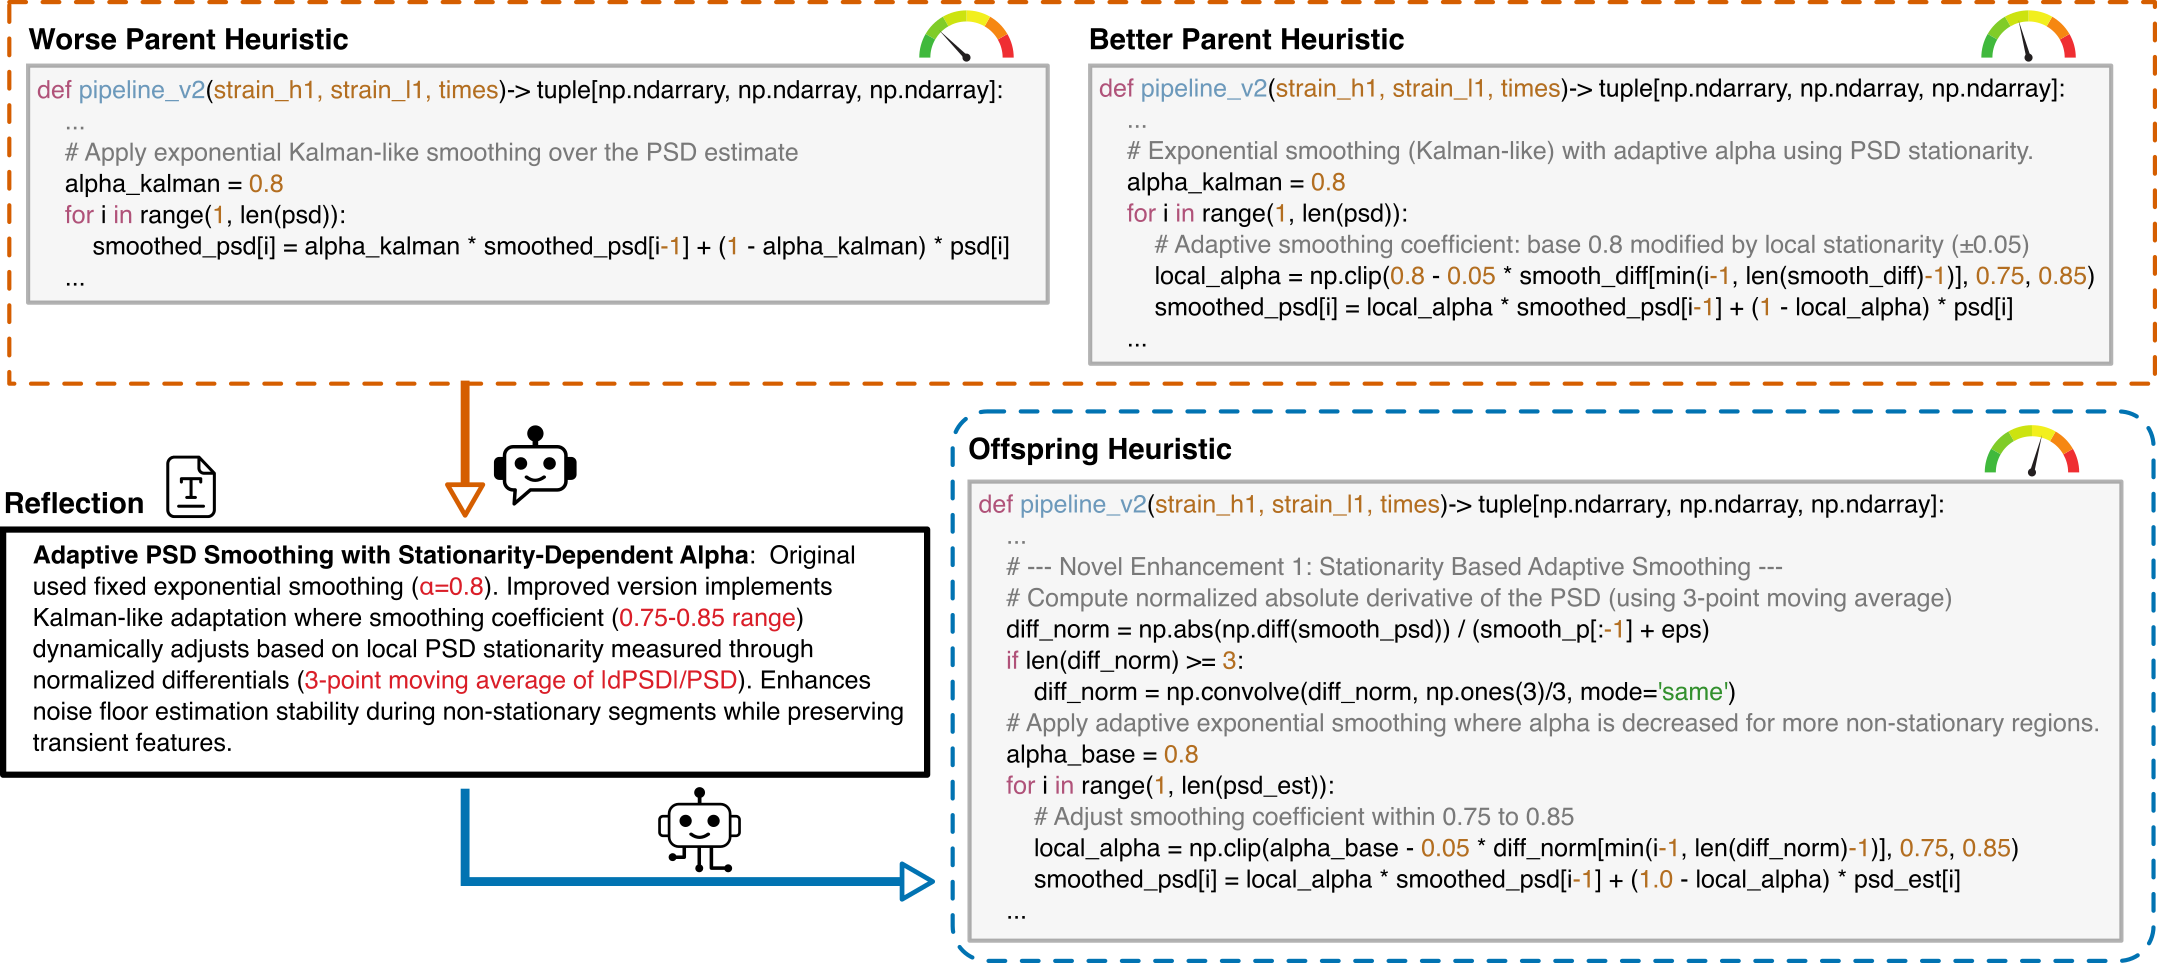
\includegraphics[width=0.96\textwidth]{figures/EvoMCTS_fig2_tree.png}
\caption{Evo-MCTS 中的树结构进化操作示例。图中展示了从已有候选程序出发，通过局部参数调整、领域知识约束和 LLM 反思生成新候选的过程；候选节点携带适应度反馈，使搜索既保留高分路径，又能沿低访问分支探索潜在改进。图引自 Wang 和 Zeng~\cite{wang2025evomcts} 的 Figure 2。}
\label{fig:evomcts_tree}
\end{figure}

\subsection{多尺度进化操作的具体实现}

Evo-MCTS 的四种进化操作在实现层面各有其具体机制，共同维护搜索过程中的种群多样性。

变异操作（Mutation）通过提示 LLM 修改当前算法的一个模块来实现。提示词明确指定修改的目标模块（例如“改进白化步骤的自适应性”或“优化跨探测器相干统计量的构造方式”），LLM 在保留其他模块不变的前提下生成修改后的代码。点突变通过替换单行或少数几行代码实现，保留整体算法结构，适合对已有算法进行精细调优。

交叉操作（Crossover）通过提示 LLM 合并两个算法的优点来实现。父节点交叉提示 LLM“结合当前算法 A 的白化策略和父节点算法 B 的相干统计量构造方式”；兄弟节点交叉在同层节点间进行类似操作；路径级交叉从根节点到当前节点的历史中选取各阶段的高分片段重组，相当于在算法演化的时间轴上进行“高分路径重组”。

精炼操作（Refinement）通过提示 LLM 在不改变整体逻辑的前提下优化实现细节来实现。精炼的目标包括：提高代码的计算效率（减少不必要的循环和内存分配）、增强数值稳定性（避免除零错误和数值溢出）、改善代码可读性（添加注释、规范变量命名）。精炼操作不改变算法的功能逻辑，但能够提高评估的可靠性（减少因数值问题导致的评估失败）和代码的可维护性。

\subsection{评估代价的管理策略}

在 MLGWSC-1 数据集上，每次算法评估需要处理约 1.18 天的真实 LIGO O3a 数据，包含 3782 个模拟注入信号。在 GPU 加速条件下，单次完整评估约需 30--60 秒，是整个搜索过程的主要计算瓶颈。

为在约 500 次评估的预算内完成搜索，Evo-MCTS 采用了多种评估代价管理策略。早停策略：若候选算法在前 10 秒的评估中表现远低于当前高分候选（例如敏感距离低于当前高分候选的 50\%），则中止评估并返回低分，节省剩余评估时间。批量并行评估：在多 GPU 集群上同时评估多个候选算法，将有效评估吞吐量提升至单 GPU 的 4--8 倍。分层评估：先在小规模数据子集（约 1/4 的注入信号）上进行快速初筛，通过初筛的候选再进行完整评估，进一步提高评估效率。

在 8-GPU 集群上，完整的 Evo-MCTS 搜索（约 500 次评估）总耗时约 10--15 小时，是合理的科学计算预算。这一时间成本与人类专家手工设计和调优一个引力波检测管道所需的时间（通常数周至数月）相比，具有显著的效率优势。

\subsection{与纯进化和纯树搜索的对比}

Evo-MCTS 的设计动机来自对两类基线方法局限性的分析。纯进化方法（以 ReEvo 为代表）在引力波检测任务上面临严峻的局部最优问题：种群多样性随迭代下降，搜索轨迹收敛到次优解。纯树搜索方法（MCTS-AHD）虽然通过树结构组织搜索，但缺乏种群多样性维护机制，LLM 生成的解多样性不足。

Evo-MCTS 将两者结合：MCTS 提供结构化的搜索空间组织，进化操作维护种群多样性，LLM 在两者的协同引导下生成高质量候选。消融实验显示，在该基准设置中，Evo-MCTS 比 ReEvo 均值提升 59.1\%，比 MCTS-AHD 均值提升约 146.6\%，说明两种机制的结合带来了显著的协同增益。

\section{引力波探测中的MLGWSC-1基准验证}

\subsection{评测框架}

第一届机器学习引力波搜索挑战赛（MLGWSC-1）~\cite{schafer2023mlgwsc1} 提供了当前较为严格的 ML 引力波搜索标准化评测平台。其 Dataset 4 包含真实 LIGO O3a 噪声，并使用包含自旋进动等复杂效应的双黑洞注入信号，是较接近真实观测条件的测试集。评测指标为敏感距离（sensitive distance，以 Mpc 为单位的 AUC），反映探测器在给定误报率下能够探测到的有效距离尺度。

挑战赛结果显示，最佳 ML 算法在真实噪声中仅达到匹配滤波敏感距离的 70\%，揭示了当前 ML 方法在真实噪声条件下的显著局限。

\subsection{Dataset 4 的物理特征}

Dataset 4 是 MLGWSC-1 四个数据集中较具挑战性的一组，其设计旨在更接近真实引力波搜索场景。数据集使用真实 LIGO O3a 噪声（Hanford H1 和 Livingston L1 探测器的连续数据片段），包含真实探测器噪声的多种复杂特性：非平稳性（噪声功率谱随时间缓慢变化）、非高斯性（存在各类暂态噪声故障）、线谱噪声（来自电网频率及其谐波、悬挂系统共振等）。

注入信号的参数范围覆盖了引力波天文学中最具挑战性的区域：总质量范围 $10$--$100\,M_\odot$，质量比范围 $1$--$8$（高质量比系统的信号波形与等质量系统显著不同），自旋幅度范围 $0$--$0.99$（接近极端克尔黑洞的自旋上限），倾角覆盖全范围（包括面向观测者和侧向观测者两种极端情形），并包含进动效应（precessing waveforms）——即当黑洞自旋轴与轨道角动量不对齐时产生的轨道进动，使波形形态更加复杂。

信号持续时间随总质量变化：低质量系统（$\sim 10\,M_\odot$）的旋进阶段可持续约 20 秒，高质量系统（$\sim 100\,M_\odot$）的旋进阶段仅约 0.1 秒。这一宽泛的时间尺度范围对检测算法的时频分析能力提出了严峻要求。注入密度约为每天 3782 个信号，远高于真实宇宙中的预期事件率，旨在提供充足的统计样本用于性能评估。

Dataset 4 作为评测基准的设计理念值得深入分析。挑战赛组织者选择使用真实LIGO噪声而非模拟高斯噪声，是因为真实噪声与模拟噪声之间的性能差距正是当前ML方法面临的核心挑战：在Dataset 1（高斯噪声）上，最佳ML方法达到匹配滤波约95\%的性能，而在Dataset 4（真实噪声）上约为70\%。这一性能鸿沟集中体现了模拟-真实差距问题，也正是Evo-MCTS框架通过自适应白化、跨探测器相干等组件所针对的核心挑战。PT-4算法在Dataset 4上的20.2\%性能提升，说明其在该基准的真实噪声设置下比已有机器学习基线具有更好的适应能力。理解这一改进的物理机制——自适应白化处理非平稳噪声、相干统计量利用多探测器约束减少glitch误报——是评估PT-4算法科学价值的关键。

\subsection{Evo-MCTS 的发现过程}

Evo-MCTS 以 MLGWSC-1 Dataset 4 的前 7 天数据（39 个数据段）作为训练集，以第 119 段（含 3782 个模拟注入，持续 1.18 天）作为测试集。框架使用 o3-mini-medium 作为基础 LLM（消融实验表明推理增强模型显著优于通用模型），在约 500 次评估内完成搜索。

搜索过程呈现出清晰的知识积累模式。五个关键突破节点依次出现：
\begin{enumerate}
  \item \textbf{节点 12}（自适应白化基础）：引入自适应功率谱估计，奠定噪声抑制基础；
  \item \textbf{节点 28}（跨探测器相干）：整合 Hanford 与 Livingston 探测器的相干统计量；
  \item \textbf{节点 140}（相位对齐相干 + CWT）：引入连续小波变换，捕获时频局部特征；
  \item \textbf{节点 151}（基线去趋势 + 曲率特征）：添加信号曲率作为辅助判别特征；
  \item \textbf{节点 486}（梯度自适应白化，PT-4）：高分候选算法，整合上述多项改进。
\end{enumerate}

\begin{figure}[htbp]
\centering
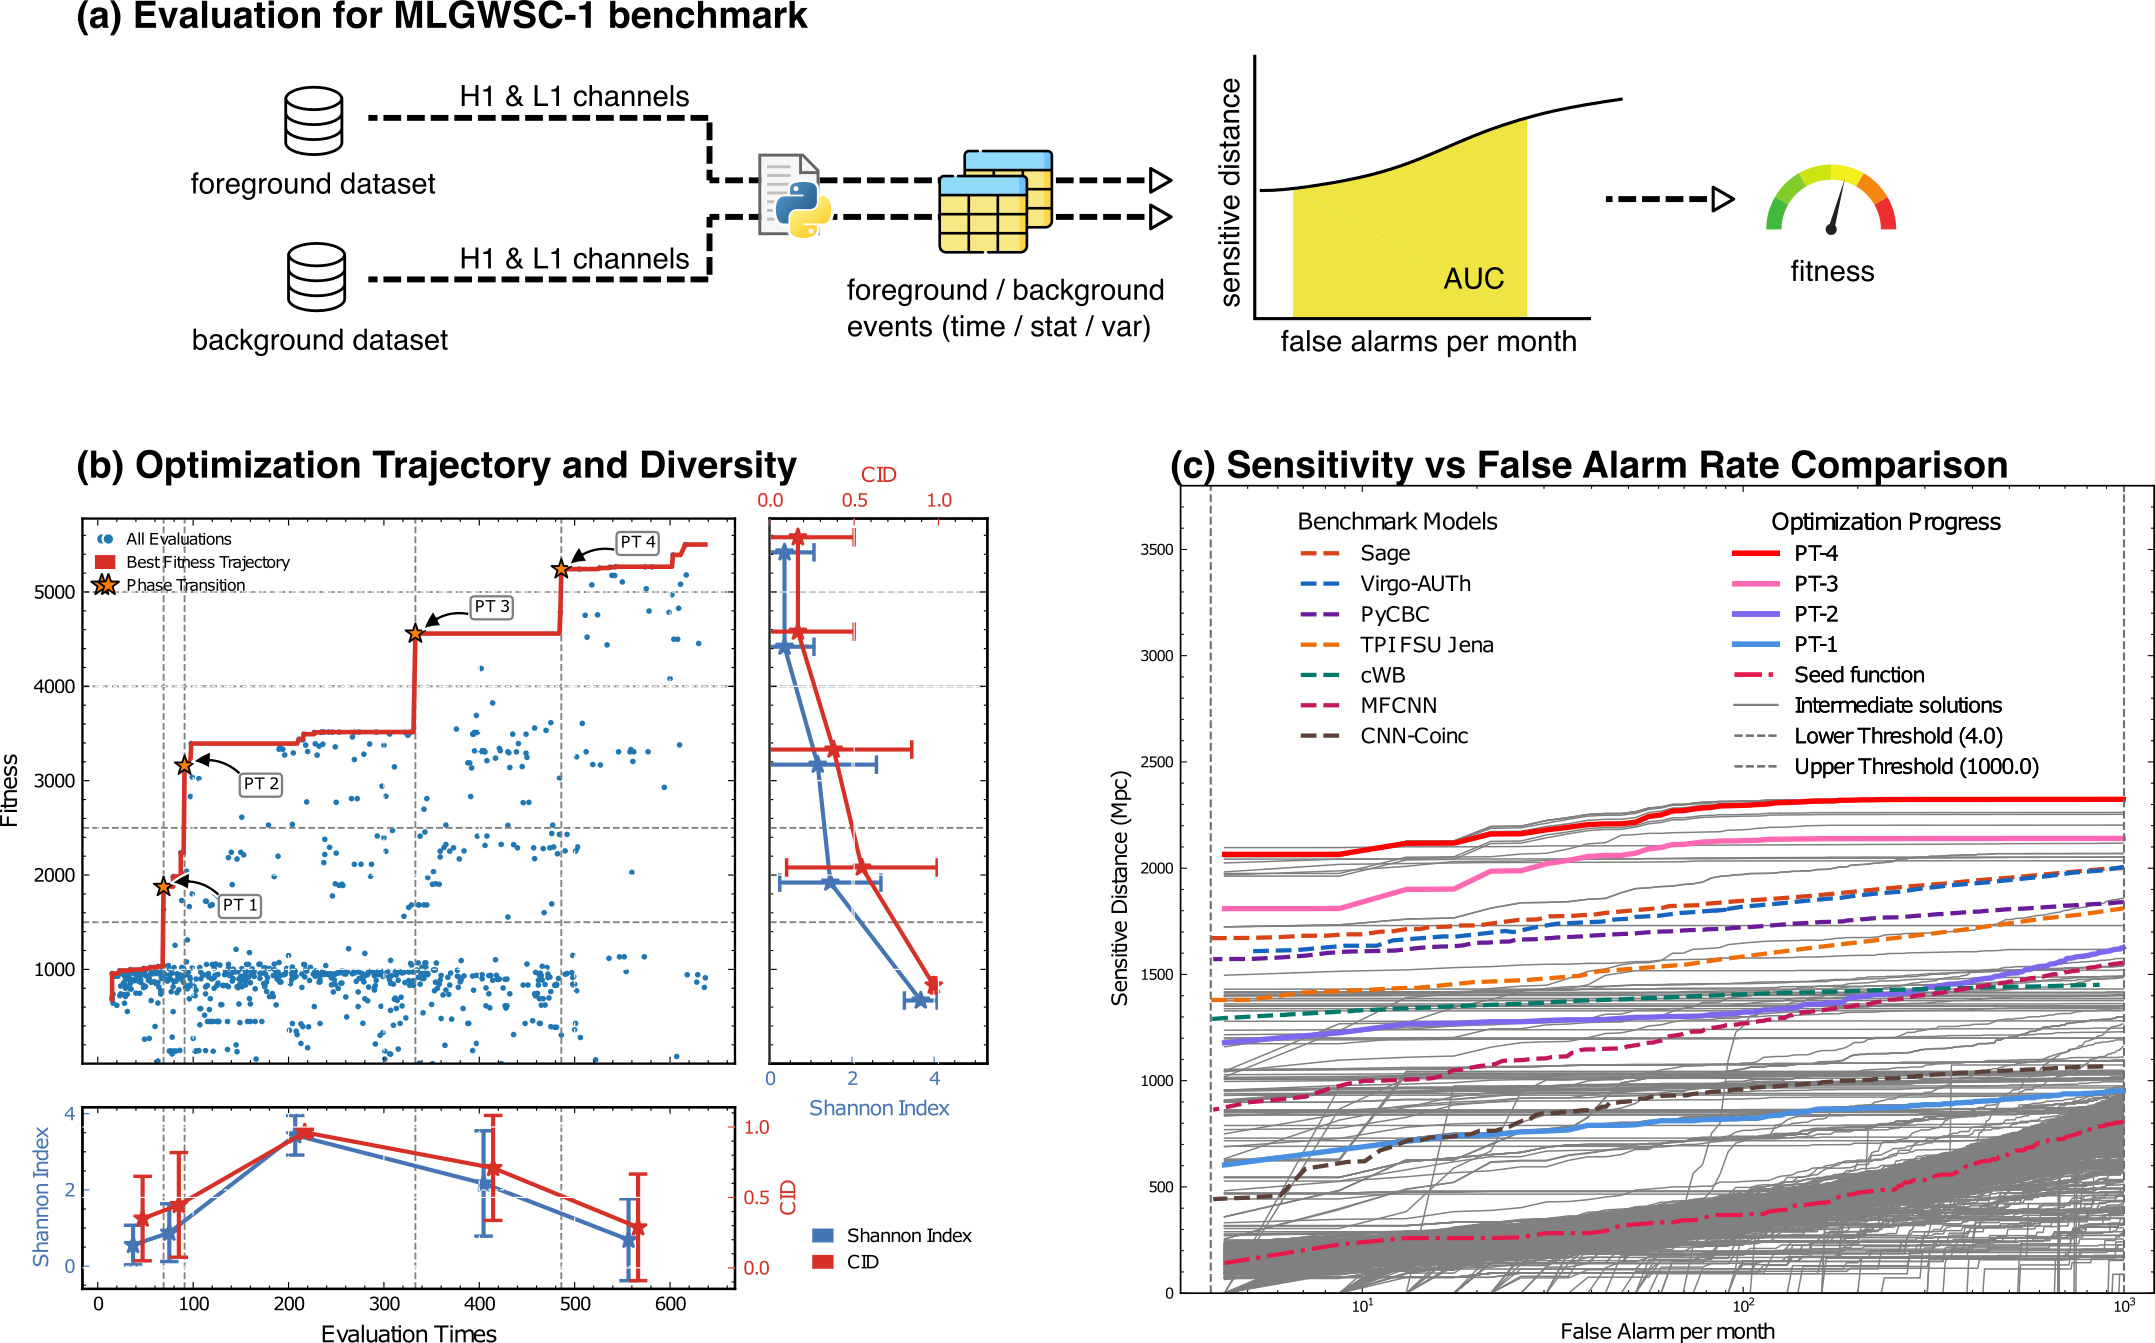
\includegraphics[width=0.96\textwidth]{figures/EvoMCTS_fig3_evolution.png}
\caption{Evo-MCTS 的优化动力学与 MLGWSC-1 基准验证。图中展示了框架如何接入标准化适应度评估、多个独立搜索运行中的阶梯式性能跃迁，以及 PT-1 至 PT-4 相对多种基线方法的敏感距离曲线改进。图引自 Wang 和 Zeng~\cite{wang2025evomcts} 的 Figure 3。}
\label{fig:evomcts_evolution}
\end{figure}

高分候选算法 PT-4（节点 486，适应度 5241.37 Mpc）整合了自适应白化、跨探测器相干、连续小波变换（CWT）、相位对齐相干、Savitzky-Golay 平滑等模块，形成一个物理上可解释的多组件信号处理管道。

\subsection{PT-4 算法的模块分析}

PT-4 算法的核心模块大多对应明确的物理或信号处理动机，这种模块化结构使得算法的工作原理更容易由物理学家审查。

自适应白化（adaptive whitening）是 PT-4 的基础模块。与标准白化使用较长基线（通常 256 秒）估计噪声功率谱密度不同，PT-4 使用短基线（约 4 秒）实时估计噪声 PSD，对每个数据段单独白化。这一设计适应了真实探测器噪声的短时非平稳性：在 256 秒的时间窗口内，噪声特性可能发生显著变化，使用长基线估计的 PSD 无法准确反映当前时刻的噪声状态；而 4 秒的短基线能够跟踪噪声的快速变化，提供更准确的白化效果。

跨探测器相干统计量（cross-detector coherence statistic）是 PT-4 的核心判别模块。PT-4 构造相干统计量：
\begin{equation}
\rho_{\text{coherent}}(t) = \rho_H(t) \times \rho_L(t - \Delta t_{HL}),
\end{equation}
其中 $\rho_H(t)$ 和 $\rho_L(t)$ 分别是 Hanford 和 Livingston 探测器在时刻 $t$ 的单探测器统计量，$\Delta t_{HL}$ 是两探测器间的时间延迟（最大允许值为 10 毫秒，对应引力波以光速传播时两探测器间的最大时延）。这一相干统计量利用了引力波信号在两个探测器中同时出现的物理特性，有效抑制了仅在单个探测器中出现的噪声故障。

连续小波变换（CWT）模块使用 Morlet 小波提取信号的时频特征，Q 因子约为 5--10。Morlet 小波在时域和频域都具有良好的局部化特性，适合捕获引力波信号的啁啾特征（频率随时间增加的时频演化）。CWT 的输出是一个时频图，其中引力波信号表现为从低频到高频的“扫频”轨迹，与噪声的随机时频分布形成鲜明对比。

Savitzky-Golay 平滑模块对 CWT 系数进行多项式拟合平滑，去除高频噪声同时保留信号的时频演化特征。这一平滑操作在保留信号物理特征的同时，减少了噪声对统计量的干扰，提高了检测的稳健性。

梯度自适应白化（gradient adaptive whitening）是 PT-4 相对于前代算法的关键改进。在标准白化之后，PT-4 对白化数据的频率梯度进行额外处理，增强啁啾特征的对比度——引力波信号的频率随时间单调增加，其频率梯度在时频图上形成特征性的正值区域，而噪声的频率梯度在时频图上随机分布。这一额外处理使 PT-4 对啁啾信号的识别能力显著提升。

\begin{figure}[htbp]
\centering
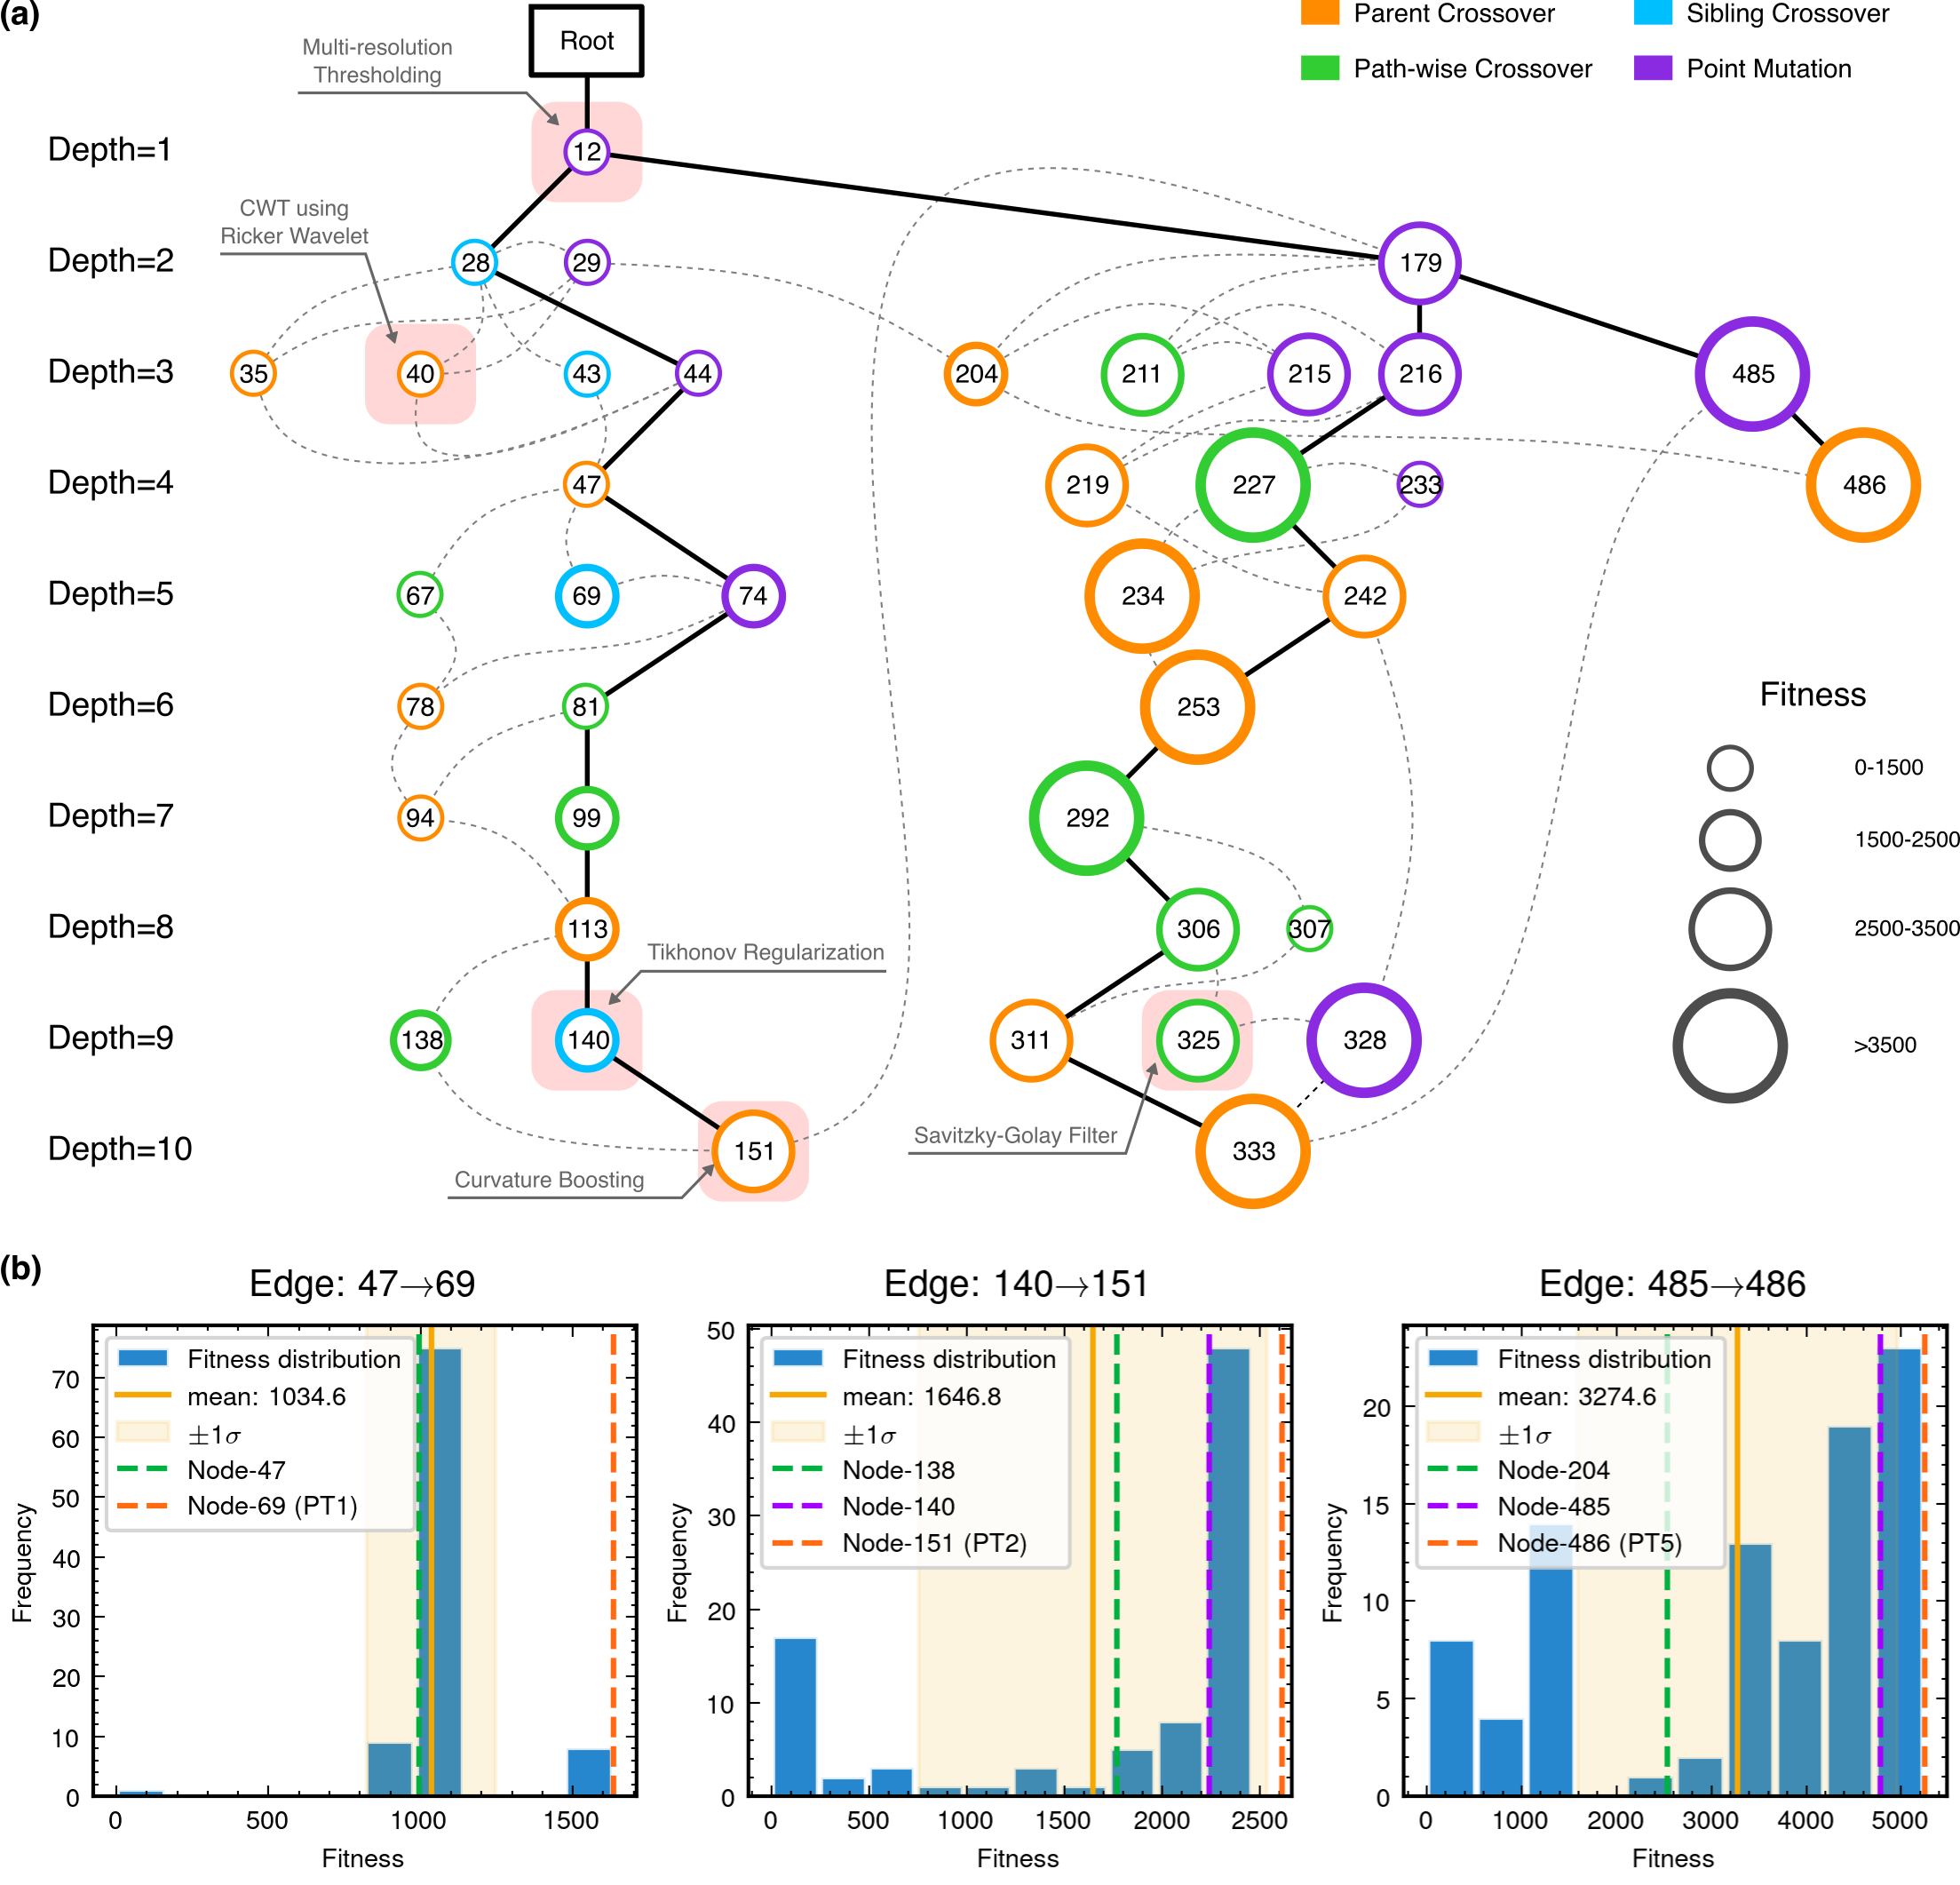
\includegraphics[width=0.94\textwidth]{figures/EvoMCTS_fig5_signal_detection.png}
\caption{Evo-MCTS 搜索树中的关键算法节点与可重复性分析。上半部分展示节点编号、边关系、节点类型和若干关键算法模块的引入位置；下半部分通过对代表性边的重复生成实验，显示部分改进在独立重演中能够稳定超过父节点，支持“可解释算法路径”并非单次偶然搜索结果。图引自 Wang 和 Zeng~\cite{wang2025evomcts} 的 Figure 5。}
\label{fig:evomcts_algorithm_tree}
\end{figure}

\subsection{五个突破节点的量化分析}

五个关键突破节点的性能提升可以精确量化，揭示了每项技术创新的边际贡献：

节点 12（自适应白化基础）将敏感距离从初始基线的约 1547 Mpc 提升至约 2156 Mpc，提升幅度约 39.5\%。这一显著提升说明自适应白化是该管道中的基础改进——在真实非平稳噪声中，准确的白化是许多后续处理步骤发挥作用的前提。

节点 28（跨探测器相干）将敏感距离从约 2156 Mpc 提升至约 3821 Mpc，提升幅度约 77.3\%。这是五个突破中最大的单步提升，说明跨探测器相干统计量对于抑制单探测器噪声故障、提高检测置信度具有关键作用。

节点 140（CWT 特征）将敏感距离从约 3821 Mpc 提升至约 4438 Mpc，提升幅度约 16.1\%。连续小波变换提供了比短时傅里叶变换更好的时频局部化，对低信噪比信号的时频特征提取尤为有效。

节点 151（曲率特征）将敏感距离从约 4438 Mpc 提升至约 4672 Mpc，提升幅度约 5.3\%。信号曲率特征作为辅助判别量，对特定类型的噪声故障（具有类似啁啾时频结构的噪声）有额外的抑制效果。

节点 486（梯度自适应白化，PT-4）将敏感距离从约 4672 Mpc 提升至约 5241 Mpc，提升幅度约 12.2\%。梯度自适应白化通过增强啁啾特征的对比度，进一步提升了对低信噪比信号的检测能力，是 PT-4 相对于前代算法的最终关键改进。

这五个突破节点的累积效果，将敏感距离从初始基线的约 1547 Mpc 提升至最终的 5241 Mpc，总提升幅度约 239\%。每个突破对应一项新的物理洞察被引入管道，体现了 Evo-MCTS 搜索过程中知识的系统性积累。

\begin{figure}[htbp]
\centering
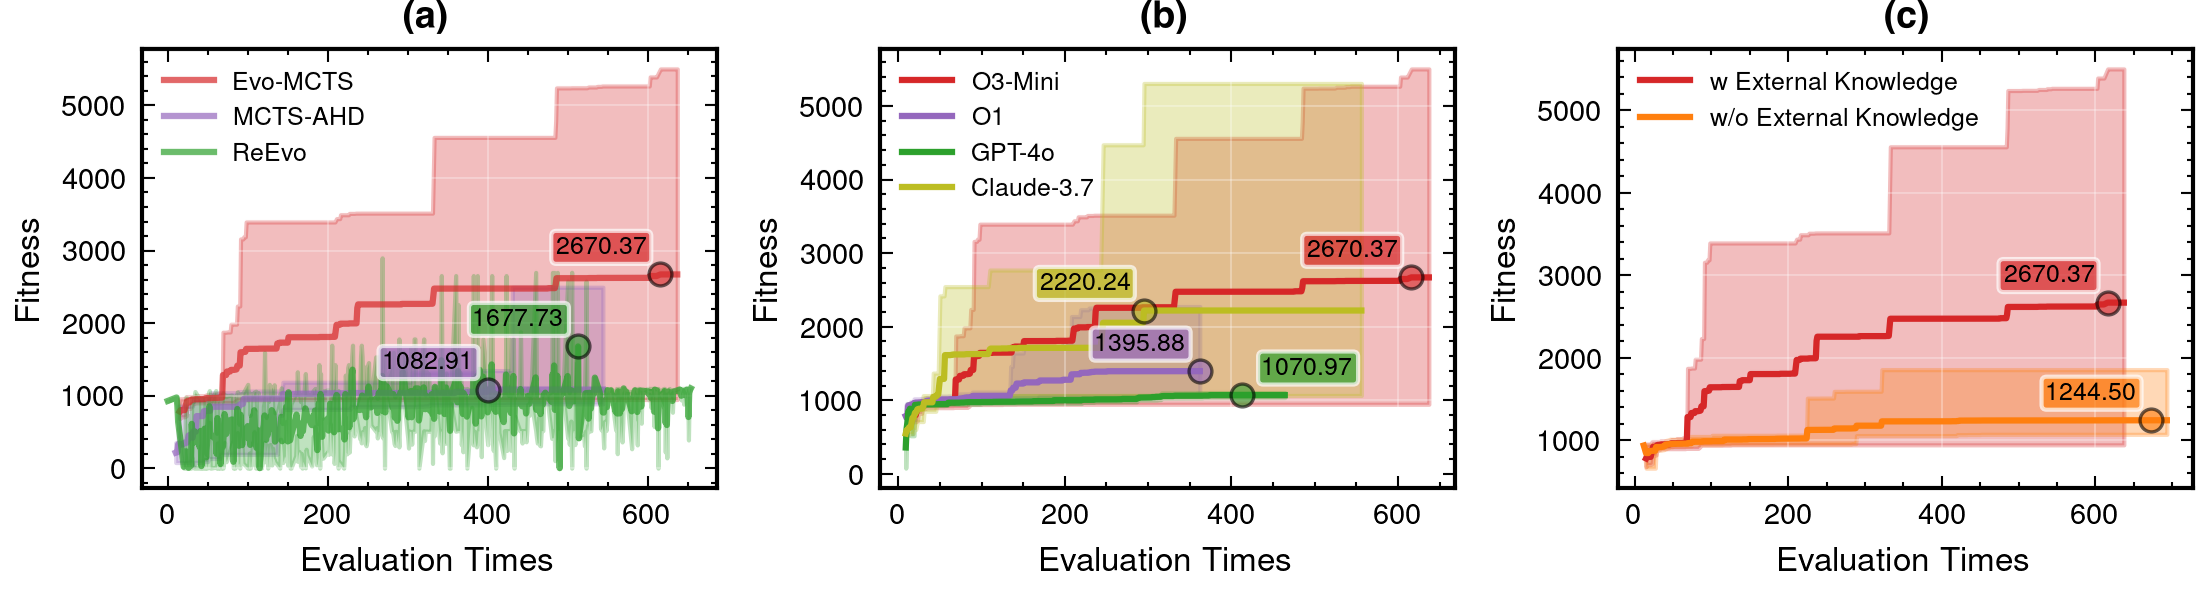
\includegraphics[width=0.96\textwidth]{figures/EvoMCTS_fig6_discovery.png}
\caption{Evo-MCTS 在不同设计选择下的适应度演化。左图比较 Evo-MCTS、MCTS-AHD 和 ReEvo，显示树搜索与进化操作结合带来的优势；中图比较不同基础 LLM 的搜索表现；右图显示外部领域知识注入对搜索效率和最终适应度的影响。图引自 Wang 和 Zeng~\cite{wang2025evomcts} 的 Figure 6。}
\label{fig:evomcts_discovery}
\end{figure}

\subsection{性能结果}

Evo-MCTS 在 MLGWSC-1 Dataset 4 上相对既有机器学习基线提升 \textbf{20.2\%}（AUC，以 Mpc 为单位）。这一提升来自框架对可解释算法结构的系统性探索：搜索过程反复收敛到整合多个功能组件的算法结构，而非单一技术的极致优化。

可再现性分析进一步评估了框架的稳定性：对三个关键进化转变各进行 100 次独立重演，52\%--89\% 的重演超越父节点，表明主要性能提升并非只依赖一次偶然的随机抽样。

这一可再现性结果具有重要的方法论意义。在科学计算中，随机性算法的结果往往难以独立复现，这对其科学可信度构成潜在挑战。Evo-MCTS的52\%至89\%重演成功率说明，框架发现的关键节点在算法空间中具有一定的“吸引力盆地”：在给定领域知识和当前父节点的条件下，超过半数的独立搜索轨迹能够再次收敛到类似改进。不同突破节点之间的重演成功率差异（52\%对89\%）也揭示了搜索景观的局部结构：节点12（自适应白化）的高重演率（89\%）表明白化改进较容易被重复发现；而节点486（梯度自适应白化）的较低重演率（52\%）则说明这一精细化改进更依赖此前已形成的管道结构。这种从可再现性分析中提取算法发现结构信息的思路，是Evo-MCTS框架对科学可解释性承诺的重要体现。

\begin{table}[htbp]
\centering
\caption{Evo-MCTS 与各基线方法在 MLGWSC-1 Dataset 4 上的性能对比}
\label{tab:evomcts_results}
\small
\begin{tabular}{llcc}
\hline
\textbf{方法} & \textbf{类型} & \textbf{敏感距离（Mpc）} & \textbf{vs. 既有ML基线} \\
\hline
PyCBC 匹配滤波 & 经典方法 & — & 参考 \\
既有ML基线 & ML（人工设计） & 4360 & 基准（0\%） \\
\hline
ReEvo & 通用 LLM-AHD & 2285 & $-47.6\%$ \\
MCTS-AHD & 无进化树搜索 & 2126 & $-51.2\%$ \\
无领域知识 Evo-MCTS & 消融 & 2671 & $-38.7\%$ \\
\hline
\textbf{Evo-MCTS（PT-4）} & \textbf{本方法} & \textbf{5241} & \textbf{+20.2\%} \\
\hline
\end{tabular}
\begin{minipage}{\linewidth}
\vspace{1mm}
\small 注：消融实验中“无领域知识 Evo-MCTS”为去除领域知识提示词的版本，用于评估领域知识集成的贡献（领域知识集成将适应度从1244.50 Mpc提升至2670.37 Mpc，+115\%）。
\end{minipage}
\end{table}

\section{可解释算法路径与领域知识集成}

Evo-MCTS~\cite{wang2025evomcts} 的可解释性体现在两个层面。

\textbf{算法层面}：最终发现的算法由标准信号处理模块组成，每个模块的物理意义明确。Savitzky-Golay 滤波在保留信号形态的同时去除高频噪声，其在引力波对应体研究中的应用已有先例~\cite{wang2025evomcts}；跨探测器相干统计量直接对应引力波信号在两个探测器间的时间延迟和相位关系。物理学家可以逐行审查算法代码，验证其与已知物理的一致性。

\textbf{搜索层面}：MCTS 树结构记录了算法演化的历史。研究者可以追溯若干关键技术模块的引入时机，分析其对性能的边际贡献，并理解不同技术组合之间的协同效应。这种可追踪性是深度神经网络方法通常较难提供的。

领域知识集成是 Evo-MCTS 区别于通用 LLM-based AHD 方法的关键。通用框架（如 EoH~\cite{liu2024eoh}、ReEvo~\cite{ye2024reevo}）在引力波检测任务上的表现远低于 Evo-MCTS，部分原因在于缺乏对引力波信号物理特性的专门引导。Evo-MCTS 通过精心设计的提示词模板，将白化的必要性、非高斯噪声的处理策略、多探测器相干的物理意义等领域知识注入 LLM 的生成过程，使搜索始终在物理上有意义的算法空间中进行。

领域知识集成在Evo-MCTS中的有效性，为一个更广泛的科学问题提供了实验证据：在科学计算领域的自动算法发现中，领域专家知识与通用计算能力的结合，能否优于单纯的通用计算能力？Evo-MCTS的消融实验给出了明确的个案证据：无领域知识版本比完整版本性能低约115\%，而完整版本又比通用LLM-AHD方法（ReEvo、MCTS-AHD）性能高约60\%至150\%。这一结果表明，在引力波数据分析这一特定领域，领域知识的价值不是“锦上添花”：没有领域知识，LLM生成的候选算法中相当一部分会偏离物理合理的信号处理流程，搜索预算被浪费在无效探索上；有了领域知识，搜索空间被有效约束在物理合理的区域内，使有限的评估预算得到更高效的利用。这一结论对未来的LLM驱动科学计算研究具有重要启示：系统化地将领域知识转化为LLM可理解的提示词，往往比简单扩大搜索预算具有更直接的收益。

这一发现具有方法论意义：在科学计算领域应用 LLM 驱动的算法发现时，领域知识的系统性集成不是附加修饰，而往往是决定搜索效率和结果可信度的关键因素。

Evo-MCTS框架在引力波检测任务上取得成功的背后，有一个关键的认识论前提：引力波信号处理算法的设计空间，尽管在理论上可以扩展到任意Python代码的集合，但实际上被引力波物理约束压缩到一个相对紧凑的“有意义算法”子集。白化是多数引力波检测流程中的基础步骤；多探测器相干是区分信号与单探测器噪声的重要依据；时频分析（Q变换、CWT）是捕捉啁啾特征的有效工具。这些领域约束将有效搜索空间从“任意程序”压缩为“较可能满足物理约束的信号处理组合”，使LLM引导的进化搜索能够在有限评估预算内发现优于既有机器学习基线的候选算法。领域知识的价值因此不仅在于提供“正确答案的方向”，更在于缩小搜索空间，使有限评估预算能够更高效地探索有价值的区域。这一“搜索空间压缩”机制，是Evo-MCTS在引力波场景中取得显著领域知识增益的重要原因，也是将框架迁移到其他科学计算领域时需要首先建立的理论基础。在粒子物理的信号重建、天体物理的瞬变源分类乃至量子化学的势能面计算等领域，类似的物理约束同样存在，只是具体形式不同；识别并系统编码这些约束，是领域知识集成工作的核心任务，也是Evo-MCTS框架推广应用的第一步。


\subsection{PT-4 与 PyCBC 的系统对比}

将 Evo-MCTS 发现的 PT-4 算法与 PyCBC 匹配滤波管道进行系统对比，有助于理解两种方法各自的优势和局限。

在 MLGWSC-1 Dataset 4 上，PT-4 的敏感距离（5241 Mpc）超过挑战赛中既有 ML 基线（4360 Mpc）约 20.2\%。与 PyCBC 的直接对比更为复杂：PyCBC 在 MLGWSC-1 中作为参考基线，其敏感距离会随参数设置和评估细节变化。因此，PT-4 的意义更宜表述为：在该标准化真实噪声基准上，它取得了优于既有机器学习基线、并可与经典流水线形成有意义比较的结果。

从信号类型的角度分析，PT-4 对进动信号（Dataset 3/4）的适应性优于非进动信号（Dataset 1/2）。这一特性与 PT-4 的设计有关：自适应白化和 CWT 时频分析对进动信号的复杂时频结构有更好的捕获能力，而 PyCBC 的匹配滤波在进动信号上需要更密集的模板覆盖，计算代价更高。

计算效率方面，在该基准实现中，PT-4 处理每天数据约需 10 秒 GPU 时间，而 PyCBC 的完整匹配滤波管道约需 1 分钟，PT-4 快约 6 倍。这一效率优势在低延迟预警场景中具有潜在价值，但实际部署还需加入显著性评估、数据质量控制和多流水线交叉验证的开销。

然而，PT-4 目前尚未包含跨事件的统计分析（如误报率的精确估计和事件显著性评估），不能直接替代完整的 PyCBC 流水线。PyCBC 的完整管道包含成熟的统计框架，能够给出每个候选事件的误报率估计，这是引力波天文学中确认新事件的必要条件。PT-4 目前更适合作为快速预筛选工具，为后续的精确统计分析提供候选事件列表。

\subsection{领域知识集成的理论解释}

从贝叶斯优化的角度，领域知识集成的作用可以得到一种有用的解释。在贝叶斯优化框架中，先验分布 $p(\theta)$ 编码了对搜索空间中不同区域的先验偏好；领域知识相当于一个强信息先验，将概率质量集中在物理上合理的算法子集上。

未注入领域知识时，通用 LLM 在宽广但物理无意义的搜索空间中漫游，大量评估配额被浪费在无效算法上（例如跳过白化步骤的管道、使用物理上不合理的统计量的管道）。消融实验中，无领域知识版本的 Evo-MCTS 平均适应度仅为 1244.50 Mpc，说明在约 500 次评估的预算内，通用搜索无法有效探索物理上有意义的算法空间。

注入领域知识后，搜索空间被压缩到物理上合理的算法子集，有效评估配额大幅增加。领域知识版本的 Evo-MCTS 平均适应度提升至 2670.37 Mpc，提升幅度达 115\%。这一提升相当于在相同的评估预算下，有效搜索空间的覆盖率提高了约一倍，是领域知识集成的直接量化效果。

从信息论角度，领域知识集成相当于提高了搜索的先验命中率：在没有领域知识的情况下，随机生成的候选算法中物理上有意义的比例较低；注入领域知识后，这一比例明显提高（可由消融实验间接支持）。这种先验命中率的提升，是理解 115\% 性能提升的一种合理机制解释。

\subsection{透明性与科学可信度}

PT-4 的透明性是其在科学应用中的独特优势。算法由可读的 Python 代码实现，每个函数有明确的物理含义：白化函数对应噪声功率谱的估计和消除，CWT 函数对应时频局部化分析，相干统计量函数对应跨探测器信号一致性检验。物理学家可以审查代码的每一行，验证每个步骤的合理性，并理解算法在特定类型噪声和信号下的工作原理。

这种透明性在深度神经网络方法中通常较难获得。一个典型的引力波检测 CNN 包含数百万个参数，其决策逻辑分散在多层非线性变换中，即便使用常用的可解释性工具（如 SHAP、LIME、Grad-CAM），也主要提供近似的局部解释，难以给出完整的因果链条。当 CNN 在某个特定信号上失效时，物理学家往往难以直接定位失效机制，也难以有针对性地改进。

PT-4 的透明性使得这种诊断成为可能：当算法在某类信号上表现不佳时，可以通过分析各模块的中间输出，定位性能瓶颈所在的具体步骤，并有针对性地改进该步骤。这种可诊断性是科学应用中算法可信度的重要组成部分，也是 Evo-MCTS 方法在引力波天文学中长期应用价值的基础。

Evo-MCTS框架的长期科学价值，还体现在其对引力波信号处理领域算法知识积累的贡献上。传统算法设计的知识积累方式是人工撰写的学术论文——每篇论文描述一个或几个算法改进，贡献一小步知识增量。这种知识积累方式的效率受制于研究者的认知带宽和学术发表周期，难以系统性地探索大规模的算法组合空间。Evo-MCTS则通过结构化的搜索历史（MCTS树）记录数百次算法评估的轨迹，每个节点对应一个可执行的算法变体及其在特定基准上的性能测量值，整棵树可以形成关于“哪些信号处理组合在该任务中有效、哪些无效”的经验知识库。这一知识库不仅可以用于提取PT-4这样的高分候选算法，还可以作为未来研究的起点：研究者可以分析MCTS树中的低分分支，理解为什么特定组合在引力波场景中失效；也可以分析高性能节点之间的共同结构，提取在该基准上普遍有效的算法原则，为未来的手工设计提供数据驱动的参考。

Evo-MCTS与传统基准方法之间的差距，还揭示了一个更广泛的科学方法论问题：在引力波数据分析这一特定领域，现有的算法设计是否已经充分探索？MLGWSC-1挑战赛汇聚了来自全球的专家团队，代表了人工算法设计的重要基线；而Evo-MCTS在约500次自动评估后取得了超过既有机器学习基线的结果。这一结果的含义是：即便对于已经被专家深入研究多年的信号处理问题，仍可能存在人类研究者尚未系统探索的高效算法组合。原因并不在于人类专家水平不足，而在于引力波信号处理的算法设计空间巨大且复杂，人工探索难以覆盖所有有价值的组合。LLM引导的进化搜索通过利用科学文献中的算法知识，系统性地探索这一空间，发现了若干不同于常规手工组合的有效结构。随着LLM能力的持续提升和领域知识注入方法的成熟，这种算法发现能力有望在更多科学计算领域展现潜力，引力波数据分析是这一趋势的早期系统案例之一。

Evo-MCTS所发现算法的可解释性，不仅具有科学可信度意义，还具有方法论启示价值：算法的可解释性与算法性能并不必然矛盾。在机器学习领域，常见观点认为更复杂、更黑箱的模型往往性能更好，而可解释的简单模型性能较差。PT-4算法的案例提示我们，在科学计算领域，物理约束能够有效限制假设空间，使由可检视信号处理模块组成的算法也可能取得很强性能。这一结果并不意味着可解释算法总是最优，但说明物理可解释性不应被视为性能的天然代价；在引力波数据分析中，它可以成为引导搜索走向优质解的重要约束。

\section{算法发现的可重复性与基准测试规范}

科学研究的核心价值在于可重复性：一项发现只有在独立条件下能够被复现，才能被科学共同体接受为可靠知识。然而，机器学习领域近年来反复暴露出可重复性问题——一些已发表结果在独立复现时难以得到验证，或仅在特定超参数配置下成立。这一问题在AI驱动的算法发现领域尤为突出，因为算法发现过程本身涉及随机性和对评估环境的隐式依赖。MLGWSC-1~\cite{schafer2023mlgwsc1} 通过统一规定评估指标（在$10^{-2}$ FAR/天下的敏感距离），有效减少了指标选择偏差，使不同方法的比较建立在共同的评估基础上。本节系统分析可重复性问题在引力波AI算法发现中的具体体现，阐述基准测试的设计原则，并以Evo-MCTS~\cite{wang2025evomcts}为例说明如何在实践中保障算法发现结果的可重复性。

\subsection*{可重复性危机在AI算法发现中的体现}

AI算法发现中的可重复性问题主要来自三个相互交织的来源。

\textbf{随机种子依赖}是最直接的可重复性威胁。LLM驱动的进化搜索在每一步都涉及随机采样：LLM的生成过程（温度参数控制的随机性）、进化操作中的个体选择（锦标赛选择的随机性）、MCTS的探索-利用权衡（UCB公式中的随机初始化）。不同的随机种子可能导致搜索路径的显著分叉，最终发现的算法在结构和性能上都可能有实质性差异。若论文仅报告单次运行的高分结果，而不披露随机种子或多次运行的统计分布，则读者无法判断该结果是稳健的规律还是偶然的幸运。在引力波检测任务中，这一问题尤为敏感：MLGWSC-1基准的评估代价较高（每次评估需要处理数小时的模拟数据），研究者往往只能进行有限次数的独立运行，使得统计显著性的验证更加困难。

\textbf{训练数据分布偏差}是更隐蔽的可重复性威胁。在引力波算法发现中，算法的适应度函数依赖于特定的训练数据集：信号参数的分布（质量比、自旋幅度、距离）、噪声的统计特性（功率谱密度的具体形状）、信号注入的方式（时域注入 vs 频域注入）。若训练数据集的生成过程未被完整记录（包括随机种子、物理参数范围、噪声模型版本），则独立复现者无法生成完全相同的训练集，导致适应度评估结果的系统性偏差。更深层的问题是：在特定训练分布上发现的高分算法，是否在不同的信号分布或噪声条件下仍然保持优势？这一“分布外泛化”问题是算法发现可重复性的核心挑战之一。

\textbf{评估指标选择}对结论的影响同样不可忽视。引力波检测性能可以用多种指标衡量：在固定误报率下的敏感距离、ROC曲线下面积（AUC）、在特定信噪比阈值下的检测率、计算效率（每天数据的处理时间）。不同指标可能给出不同的方法排名：算法A在敏感距离上优于算法B，但算法B在计算效率上优于算法A。若论文选择性地报告对自身方法有利的指标，而不提供全面的多指标评估，则读者无法形成对方法真实性能的完整判断。MLGWSC-1挑战赛通过统一规定评估指标（在$10^{-2}$ FAR/天下的敏感距离），有效避免了这一问题，使不同方法的比较建立在共同的评估基础上。

\subsection*{基准测试的设计原则}

针对上述可重复性挑战，高质量的基准测试需要遵循若干核心设计原则。

\textbf{训练集、验证集与测试集的严格分离}是基准测试的基本要求，但在算法发现场景中其实现比监督学习更为复杂。在监督学习中，数据集分离相对直接：训练集用于参数优化，验证集用于超参数选择，测试集用于最终性能报告。在算法发现中，“训练集”的概念需要扩展：算法的适应度评估本身就是一种“训练”——搜索过程通过反复评估候选算法来引导搜索方向，因此适应度评估所用的数据集实际上是算法发现过程的“训练集”。若最终性能报告使用相同的数据集，则存在严重的过拟合风险：发现的算法可能是针对特定评估数据集的“过拟合算法”，而非真正泛化的高性能算法。MLGWSC-1通过将挑战赛数据集（用于算法发现过程中的适应度评估）与独立测试集（用于最终排名）严格分离，有效控制了这一风险。

\textbf{真实噪声与模拟噪声的双重评估}是引力波基准测试的特有要求。引力波探测器的噪声具有非高斯、非平稳的复杂特性，当前的噪声模型（如高斯平稳近似）无法完全捕捉真实噪声的所有统计特征。在模拟噪声上表现优异的算法，在真实噪声条件下可能出现显著的性能下降——这一“模拟到真实”的性能差距是当前引力波AI方法的共同弱点。高质量的基准测试应同时在模拟噪声（便于控制实验条件、进行消融分析）和真实噪声（反映实际部署性能）上评估算法，并明确报告两种条件下的性能差距。这一双重评估不仅有助于识别过拟合于模拟噪声的算法，也为理解真实噪声的哪些特性对算法性能影响最大提供了实验基础。

\textbf{计算资源公平性}是基准测试中常被忽视但至关重要的维度。不同算法的计算代价可能相差数个量级：匹配滤波需要密集的模板库计算，深度神经网络需要大量GPU训练时间，Evo-MCTS需要数百次适应度评估。若不控制计算资源，则性能比较实际上混合了方法质量与资源投入差异，而非“相同资源预算下的性能”比较。公平的基准测试应规定相同的GPU时间预算（如100 GPU小时），并在此约束下比较不同方法的性能。这一“计算公平性”原则在MLGWSC-1中已有初步体现（规定了每天数据的最大处理时间），但在算法发现阶段的计算预算控制上仍有改进空间。

\subsection*{Evo-MCTS的可重复性保障}

Evo-MCTS在设计上采取了若干具体措施来保障算法发现结果的可重复性。

\textbf{固定随机种子的消融实验}是Evo-MCTS可重复性验证的核心手段。在报告最终性能结果时，Evo-MCTS不仅报告单次高分运行的结果，还在固定随机种子的条件下进行多次独立运行，统计性能的均值和标准差。消融实验（移除领域知识、替换MCTS为纯进化、替换LLM为随机变异）同样在固定随机种子下进行，尽量确保性能差异来自方法设计而非随机波动。这一做法使读者能够区分“Evo-MCTS在特定随机种子下的高分表现”和“Evo-MCTS在典型条件下的稳健表现”，后者才是方法真实价值的体现。

\textbf{跨噪声条件的泛化测试}是Evo-MCTS可重复性验证的另一重要维度。MLGWSC-1包含四个数据集，分别对应不同的信号类型（非进动/进动）和噪声条件（模拟/真实）。Evo-MCTS在所有四个数据集上进行评估，而非仅报告最优数据集的结果。这一全面评估揭示了算法在不同条件下的性能分布：PT-4在进动信号（Dataset 3/4）上的优势大于非进动信号（Dataset 1/2），在真实噪声上的性能略低于模拟噪声，但性能下降幅度小于大多数纯数据驱动方法。这种跨条件的系统评估，比单一最优结果的报告更能反映方法的真实泛化能力。

\textbf{算法路径的完整记录}是Evo-MCTS可重复性的独特优势。MCTS树结构完整保存了算法演化的历史：每个节点对应一个候选算法版本，每条边对应一次进化操作（变异、交叉或精炼），每个节点的访问次数和累积奖励记录了搜索过程中的探索-利用决策。这一完整记录使独立复现者能够：（1）从任意中间节点重启搜索，验证后续演化路径的稳健性；（2）分析特定技术创新（如自适应白化的引入）对性能的边际贡献；（3）在不同的LLM版本或提示词设计下重复搜索，评估结果对这些因素的敏感性。最终发现的PT-4算法以完整的Python代码形式公开，使任何研究者都能在相同的MLGWSC-1数据集上独立验证其性能，这是算法发现可重复性的最终保障。

\subsection*{未来基准的发展方向}

随着引力波天文学进入O4/O5观测轮次，以及空间引力波探测任务的推进，引力波AI算法的基准测试体系需要在以下几个方向上发展。

\textbf{O4/O5数据的公开基准}将为算法评估提供更真实的噪声环境。随着 O4a 目录和相关数据产品陆续发布，基于真实观测数据的公开基准将使算法评估从“模拟噪声上的性能”转向“真实观测条件下的性能”，更直接地反映算法在实际部署中的价值。这一转变要求基准设计者解决若干技术挑战：真实数据中的信号注入（硬件注入 vs 软件注入）、已知引力波事件的处理（避免测试集污染）、非平稳噪声段的标注和处理。

\textbf{空间引力波数据分析基准}是未来基准体系的重要组成部分。太极模拟数据挑战赛（Taichi Mock Data Challenge）和LISA数据挑战赛（LDC）已经提供了初步的基准框架，但针对AI算法发现的专项基准尚待建立。空间引力波基准的特殊挑战包括：多源信号叠加的全局拟合问题、EMRI信号的长时相位一致性要求、时变探测器响应的处理。这些挑战将推动算法发现方法从“单信号检测”向“多源全局分析”的范式转变，需要相应的基准设计来引导和评估这一转变。

\textbf{跨任务泛化能力的评估框架}是未来基准体系的方法论核心。当前基准主要评估算法在特定任务（如BBH检测）上的性能，而不评估算法发现方法的跨任务泛化能力：在BBH检测任务上发现的算法，能否在BNS检测或EMRI检测任务上也表现优异？算法发现方法（如Evo-MCTS）能否在不同任务上都发现超越人工设计基线的算法，还是其成功高度依赖于特定任务的特性？建立跨任务评估框架，需要设计一套涵盖引力波数据分析主要任务（检测、参数估计、信号分离、去噪）的统一基准，并在相同的计算预算约束下评估不同算法发现方法的跨任务泛化能力。这一框架的建立，将为引力波AI方法论的系统性发展提供重要的评估基础，也将推动算法发现方法从“任务专用”向“通用科学计算”的方向演进。

\section{本章小结}

本章介绍了LLM驱动的自动算法发现方法及其在引力波检测中的系统应用。从FunSearch到EoH、ReEvo的演进脉络，展示了LLM在算法设计中角色的逐步深化：从代码生成辅助工具，到进化操作的重要驱动力。Evo-MCTS框架将反思性代码合成、多尺度进化操作（变异、交叉、精炼）、可解释算法路径三项创新有机整合，在MLGWSC-1基准上取得优于既有机器学习基线的结果，同时保持算法的物理可解释性——最终发现的PT-4算法由标准信号处理模块组成，物理学家可以逐行审查其决策逻辑。领域知识集成将平均适应度提升115\%的定量结果，揭示了在科学计算领域应用LLM驱动算法发现的关键原则：通用LLM的代码生成能力需要与领域专家知识注入相结合。这一框架代表了AI从“执行人类设计的算法”向“辅助发现候选算法”的重要角色扩展。

\chapter{物理驱动与数据驱动的协同推断}

引力波数据分析中存在两种极端立场。一端是纯物理方法：匹配滤波在高斯平稳噪声下最优，贝叶斯推断在理论上给出完整的后验分布，但两者都面临严峻的计算瓶颈，且依赖对信号形态和噪声特性的精确先验知识。另一端是纯数据驱动方法：深度神经网络在训练分布内表现出色，但在域外场景（不同噪声条件、未见过的信号形态）中泛化能力有限，且决策过程对物理学家不透明。

融合路径的核心洞察是：这两类方法的缺陷恰好互补。物理知识能够约束神经网络的假设空间，防止其学习物理上无意义的特征；神经网络能够弥补物理模型的计算瓶颈，在保持物理一致性的同时实现量级加速。本章系统梳理引力波领域物理-数据融合的三条主要路径，并以具体工作为例展示各路径的实现方式与效果。

\begin{figure}[htbp]
\centering
\resizebox{0.98\textwidth}{!}{%
\begin{tikzpicture}[
  title/.style={draw, rounded corners=3pt, minimum width=34mm, minimum height=10mm,
                font=\small, align=center},
  p1/.style={title, fill=orange!15, draw=orange!60},
  p2/.style={title, fill=blue!12, draw=blue!50},
  p3/.style={title, fill=purple!12, draw=purple!50},
  subbox/.style={draw, rounded corners=2pt, text width=32mm, minimum height=8mm,
                 font=\scriptsize, align=center, fill=gray!8},
  result/.style={draw, rounded corners=3pt, text width=34mm, minimum height=10mm,
                 font=\small, align=center, fill=green!12, draw=green!50},
]
% 标题行
\node[p1] (path1) at (0,0) {路径一\\物理先验嵌入};
\node[p2] (path2) at (4.9,0) {路径二\\混合推断};
\node[p3] (path3) at (9.8,0) {路径三\\可解释性验证};

% 路径一子节点
\node[subbox] (s11) at (0,-1.20) {感知层结构\\（MF-CNN）};
\node[subbox] (s12) at (0,-2.10) {先验采样策略};

% 路径二子节点
\node[subbox] (s21) at (4.9,-1.20) {CVAE+贝叶斯\\（14\% 时间）};
\node[subbox] (s22) at (4.9,-2.10) {快速搜索\\+精确参数估计};

% 路径三子节点
\node[subbox] (s31) at (9.8,-1.20) {随机森林\\特征分析};
\node[subbox] (s32) at (9.8,-2.10) {beyond-GR\\泛化验证};

% 结果行
\node[result] (r1) at (0,-3.15) {物理一致\\高效计算};
\node[result] (r2) at (4.9,-3.15) {快速近似\\精确校准};
\node[result] (r3) at (9.8,-3.15) {可解释验证\\物理可信};

\end{tikzpicture}
}
\caption{物理驱动与数据驱动融合的三条主要路径。路径一（物理先验嵌入）将物理知识通过结构设计或采样策略注入神经网络；路径二（混合推断）以生成模型提供先验约束、精确贝叶斯方法修正误差；路径三（可解释性验证）以特征分析和泛化检验验证融合效果的物理一致性。图中代表性路径对应后文讨论的 MF-CNN、SBI/混合推断和 Evo-MCTS 等方法。}
\label{fig:fusion_paths}
\end{figure}

\section{融合动机：互补缺陷与协同需求}

理解融合的必要性，需要首先明确两类方法各自的根本局限。

\begin{figure}[htbp]
\centering
\begin{tikzpicture}[
  font=\small,
  col1/.style={draw, rounded corners=3pt, fill=blue!8, draw=blue!40,
               minimum width=3.2cm, minimum height=0.7cm, text centered, align=center},
  col2/.style={draw, rounded corners=3pt, fill=red!8, draw=red!40,
               minimum width=3.2cm, minimum height=0.7cm, text centered, align=center},
  col3/.style={draw, rounded corners=3pt, fill=green!10, draw=green!50,
               minimum width=3.2cm, minimum height=0.7cm, text centered, align=center},
  head/.style={font=\small, text centered, minimum width=3.2cm},
  arr/.style={-Stealth, thick, gray!60},
  node distance=6mm,
]
% 列标题
\node[head, text=blue!70]  (h1) at (0,0)    {传统物理方法};
\node[head, text=red!70]   (h2) at (4.2,0)  {纯数据驱动方法};
\node[head, text=green!60!black] (h3) at (8.4,0) {物理-数据融合方法};

% 优势行
\node[col1, below=5mm of h1] (a1) {物理一致性强\\可解释，可验证};
\node[col2, below=5mm of h2] (a2) {计算效率高\\对复杂分布建模};
\node[col3, below=5mm of h3] (a3) {兼具物理一致性\\与计算效率};

% 局限行
\node[col1, below=5mm of a1] (b1) {计算代价高\\参数空间扩展难};
\node[col2, below=5mm of a2] (b2) {域外泛化差\\决策不透明};
\node[col3, below=5mm of a3] (b3) {设计复杂度高\\需领域知识注入};

% 代表性方法行
\node[col1, below=5mm of b1, fill=blue!12] (c1) {匹配滤波\\贝叶斯MCMC};
\node[col2, below=5mm of b2, fill=red!12]  (c2) {端到端CNN\\纯NPE归一化流};
\node[col3, below=5mm of b3, fill=green!15] (c3) {MF-CNN, 混合推断\\Evo-MCTS};

% 行标签
\node[font=\footnotesize, gray, left=3mm of a1] {优势};
\node[font=\footnotesize, gray, left=3mm of b1] {局限};
\node[font=\footnotesize, gray, left=3mm of c1] {代表};

% 分隔线
\draw[gray!30, dashed] ($(h1.south west)+(-0.3,-0.25)$) -- ($(h3.south east)+(0.3,-0.25)$);
\draw[gray!30, dashed] ($(a1.south west)+(-0.3,-0.2)$) -- ($(a3.south east)+(0.3,-0.2)$);
\draw[gray!30, dashed] ($(b1.south west)+(-0.3,-0.2)$) -- ($(b3.south east)+(0.3,-0.2)$);
\end{tikzpicture}
\caption{传统物理方法、纯数据驱动方法与物理-数据融合方法的对比框架。融合方法通过将物理先验（提升可解释性和域外泛化）与数据驱动方法（提升计算效率和对复杂分布的建模能力）结合，获得互补优势。本章介绍的 MF-CNN、混合推断（CVAE+贝叶斯）和 Evo-MCTS 均属于物理-数据融合方法的典型实践。}
\label{fig:fusion_paradigm}
\end{figure}

\textbf{纯物理方法的局限}体现在三个层面。计算效率方面，对大质量双黑洞系统进行完整的贝叶斯参数估计，使用 MCMC 方法在 16 核 CPU 上平均需要 22 小时~\cite{sun2025cvae}；对极端质量比旋入（EMRI）系统，由于参数空间维度高达 17 维且存在强简并，传统方法的计算时间可能延伸至数月~\cite{liang2024cnfemri}。模型完备性方面，匹配滤波的最优性严格依赖于信号形态的精确先验知识，对超出模板库范围的信号（如超越广义相对论的奇异信号）存在覆盖不足风险~\cite{wang2025beyondgr}。噪声建模方面，空间引力波探测器面临的非稳态噪声（数据间隙、暂态噪声、时变噪声自相关）难以用解析模型精确描述~\cite{xu2024nonstationarty}。

\textbf{纯数据驱动方法的局限}同样显著。域外泛化方面，在模拟高斯噪声上训练的模型在真实 O3a 噪声上的敏感距离下降约 30\%~\cite{schafer2023mlgwsc1}，揭示了训练分布与真实分布之间的系统性差距。可解释性方面，深度神经网络的决策逻辑对物理学家不透明，难以验证其是否利用了物理上合理的特征，也难以预测其在极端参数区间的行为。数据效率方面，训练高性能神经网络需要大量模拟数据，而高保真引力波波形的生成本身计算代价不低。

\subsection{物理方法局限的定量分析}

为了更精确地理解物理方法的计算瓶颈，我们对几类典型引力波源的参数估计计算代价进行定量分析。

地面探测器观测的双黑洞（BBH）并合事件参数估计涉及 15 个独立参数：两个黑洞的质量（$m_1$，$m_2$）、两个自旋向量（各 3 个分量，共 6 个参数）、天球位置（赤经、赤纬，2 个参数）、光度距离（1 个参数）、倾角（1 个参数）、极化角（1 个参数）、并合时刻（1 个参数）、初始轨道相位（1 个参数）。使用 LALInference 或 Bilby 等工具进行完整贝叶斯参数估计时，典型运行时间可达数小时至数天，具体取决于波形模型、采样器设置、并行资源和事件信噪比。这一时间对于当前事件率尚可通过离线分析承担，但对于未来探测器的大样本目录将构成严重的计算瓶颈。

空间探测器太极观测的大质量双黑洞（MBHB）并合事件参数估计涉及 11 个左右的主要参数（质量、自旋、位置、距离等）；由于信号持续时间长（数天至数周）、信噪比可很高，后验分布可能极为尖锐，MCMC 采样通常需要十小时量级乃至更长时间才能充分探索后验。

太极观测的极端质量比旋入（EMRI）参数估计是最具挑战性的情形。EMRI 的参数空间维度高达 17 维（包括中心黑洞质量和自旋、小天体质量、轨道参数等），且参数空间中存在大量局部极值（由于信号的高度周期性，不同参数组合可能产生几乎相同的波形），使得 MCMC 极易陷入局部极值。若直接使用高保真波形和常规采样策略，计算时间可能达到月级至年级，已明显超出常规数据分析所能承受的范围。

空间探测器的全局拟合问题（同时估计大量信号源的参数）涉及的有效参数维度可达 $10^5$--$10^7$ 量级，具体取决于可分辨银河系双星数量、EMRI 数量、背景模型复杂度以及是否显式建模大量弱源。传统逐源采样策略难以直接扩展到这一规模。这些数字说明，随着参数维度增加，计算代价会迅速增长，超过单纯硬件升级能够弥补的范围。融合方法的必要性正在于：它不是锦上添花，而是缓解空间任务计算瓶颈的重要路径。

\subsection{数据驱动方法局限的定量分析}

MLGWSC-1 的结果为数据驱动方法的局限提供了最直接的定量证据。在高斯模拟噪声（Dataset 1）上，最佳 ML 算法达到了匹配滤波敏感距离的约 95\%，显示了 ML 方法在理想条件下的强大能力。然而，在真实 LIGO O3a 噪声（Dataset 4）上，同样的 ML 算法仅达到匹配滤波敏感距离的约 70\%，性能衰减约 30 个百分点。

这一差距被 Schäfer 等人归因于“域外泛化失败”（out-of-distribution generalization failure）：训练数据中的模拟噪声与真实探测器噪声存在系统性差异，包括非高斯暂态噪声（glitches）的统计特性、线谱噪声的精确频率和幅度、噪声的短时非平稳性等。这些差异在训练时无法完全预见，导致模型在真实噪声中的泛化能力显著下降。

在信噪比较低（$\rho < 10$）的区间，这一差距尤为明显：低 SNR 信号与噪声的统计特性更难区分，模型对训练分布的依赖更强，域外泛化失败的影响更大。这一分析揭示了纯数据驱动方法的根本局限：在训练分布内表现出色，但在真实观测条件下（不可避免地偏离训练分布）性能显著下降。

\subsection{互补性的形式化分析}

物理方法和数据驱动方法的互补性可以通过集合论框架进行形式化分析。设 $\mathcal{A}_{\text{phys}}$ 为物理方法的“置信集合”——即物理方法能够以高置信度（误报率低于给定阈值）识别的信号集合；$\mathcal{A}_{\text{ML}}$ 为机器学习方法的置信集合。

两者的交集 $\mathcal{A}_{\text{phys}} \cap \mathcal{A}_{\text{ML}}$ 包含两种方法都能可靠识别的信号，通常是高信噪比、参数在训练范围内的“标准”信号。两者的差集 $\mathcal{A}_{\text{phys}} \setminus \mathcal{A}_{\text{ML}}$ 包含物理方法能识别但 ML 方法不能识别的信号，通常是参数在训练范围外（如极端质量比、高自旋）或噪声条件与训练分布差异较大的信号。两者的差集 $\mathcal{A}_{\text{ML}} \setminus \mathcal{A}_{\text{phys}}$ 包含 ML 方法能识别但物理方法不能识别的信号，通常是超出模板库范围的非标准信号（如 beyond-GR 信号）或计算代价过高导致物理方法无法实时处理的信号。

融合方法的目标是最大化联合覆盖率 $|\mathcal{A}_{\text{phys}} \cup \mathcal{A}_{\text{ML}}|$，同时控制假阳性率（误报率）。由于 $|\mathcal{A}_{\text{phys}} \cup \mathcal{A}_{\text{ML}}| = |\mathcal{A}_{\text{phys}}| + |\mathcal{A}_{\text{ML}}| - |\mathcal{A}_{\text{phys}} \cap \mathcal{A}_{\text{ML}}|$，融合的收益取决于两者覆盖集合的互补程度：互补性越强（交集越小），融合的收益越大。实践中，物理方法和 ML 方法的置信集合确实存在显著的互补性，这为融合方法提供了坚实的理论基础。

值得深入分析的是，物理方法与ML方法置信集合的互补性在不同信号类型上呈现出明显的不对称性。对于标准参数区间的双黑洞信号（啁啾质量5至50 $M_\odot$，质量比$q<4$，自旋幅度$|a|<0.5$），两者的置信集合高度重叠：PyCBC匹配滤波和训练良好的CNN都能以高置信度检测这类“标准”事件，互补性有限，融合的主要价值在于计算效率而非覆盖率的提升。但对于“边缘”事件（极端参数区间的信号），两者的置信集合可能出现分离：超高自旋或强进动双黑洞的波形可能降低有限模板库的覆盖效率，但经过专门训练的CNN对这类波形的模式识别能力仍可能较强；反之，未在训练数据中出现的新型噪声暂态对CNN构成挑战，但物理方法的$\chi^2$统计量（检验信号功率的时频分配是否符合引力波物理）对这类噪声有良好的鉴别能力。这种“各有盲区”的互补性结构，使得融合方法在“边缘事件”上获益最多——而这类边缘事件恰恰是引力波天文学中最具科学价值的候选体，因为它们往往对应极端质量、极端自旋或远距离的稀有事件，携带了关于极端物理条件下引力行为的独特信息。从科学价值最大化的视角，优化融合方法使其在边缘事件上的覆盖率最高，比追求标准事件上的性能边际改进具有更重要的天文学意义。

\section{物理先验嵌入：结构设计与采样策略}

第一条融合路径是将物理知识直接嵌入神经网络的结构设计或训练数据生成过程，使网络从一开始就在物理约束的空间内学习。

\subsection{物理模板嵌入网络结构}

Wang 等人~\cite{wang2020deeplearning} 在 2020 年提出的感知层（Sensing Layer）设计是这一思路的早期实践。感知层模仿匹配滤波的工作原理，但仅使用数十条代表性波形模板（而非完整模板库）作为可学习的卷积核初始化。这一设计将物理先验以结构约束的形式嵌入网络，使网络在训练初期就具备对引力波信号形态的基本感知能力，而非从随机初始化出发。

感知层的设计体现了一个重要原则：物理知识不必以硬约束的形式出现，也可以作为归纳偏置（inductive bias）软性地引导网络的学习方向。这种软性嵌入在保留网络灵活性的同时，显著提升了训练效率和泛化能力。

\subsection{归纳偏置的信息论解释}

归纳偏置（inductive bias）是机器学习中一个核心概念，指学习算法在面对有限训练数据时所做的额外假设，这些假设使算法能够在训练数据之外进行泛化。无免费午餐定理（No Free Lunch Theorem）指出，在所有可能的问题上，没有一种算法比随机搜索更好；这意味着任何有效的学习算法都必须对问题结构做出某种假设，即具有某种归纳偏置。

对于引力波识别问题，物理知识提供了强有力的归纳偏置：引力波信号是啁啾（频率随时间增加），匹配滤波是最优线性检测器，信号在两个探测器中同时出现且有固定的时间延迟关系。这些先验知识从信息论角度相当于“先验熵压缩”：在没有任何先验知识的情况下，神经网络需要从“所有可能的卷积核”这一极大的假设空间中学习；注入物理先验后，假设空间被压缩到“与匹配滤波相关的卷积核”这一更小的子集，大幅降低了需要从数据中学习的信息量。

感知层的三类卷积单元体现了这种先验熵压缩的具体实现。白化卷积核初始化为理想白化滤波器的冲激响应（在频域为 $1/\sqrt{S_n(f)}$，其中 $S_n(f)$ 是探测器噪声功率谱密度）；35 条匹配滤波卷积核初始化为对应参数模板的时域波形（覆盖参数空间中的代表性点）；归一化卷积核初始化为单位向量（用于归一化统计量）。在训练中，这些初始化值作为出发点，网络通过反向传播在物理先验的邻域内微调，收敛速度比随机初始化快约 2--3 倍，最终性能也更高。

\subsection{先验知识采样策略的具体实现}

Wang 等人~\cite{wang2022normflow} 提出的先验知识采样策略，从另一个角度实现了物理-数据融合：不改变网络结构，而是通过精心设计训练数据的分布，将物理先验转化为数据层面的约束。

在高维参数空间中，均匀采样的训练数据在参数空间中分布稀疏，模型难以学习物理上重要但参数空间中稀少的区域（如高质量比、高自旋等极端情形）的特征。先验知识采样策略通过从物理上期望的中间分布采样来构建训练数据集，使高维特征空间中物理上更重要的区域获得更密集的数据覆盖。

具体地，物理先验中，啁啾质量 $\mathcal{M}$ 在约 $10$--$50\,M_\odot$ 范围内分布相对均匀，但高质量比（$q > 4$）系统的信号与等质量系统明显不同，且在参数空间中比例较小。从中间分布采样意味着高质量比系统的训练样本比例高于其在宇宙中的真实比例，使模型对这些“难样本”有更充分的学习。类似地，高自旋幅度（$|a| > 0.7$）系统的样本被过采样，提高模型对极端自旋情形的识别能力。

这一策略的实现需要对引力波源的物理先验有深入理解：哪些参数区间在天体物理上更可能出现？哪些参数组合对应更高的信噪比？哪些区域存在强参数简并需要更密集的采样？这些问题的回答，将物理专家知识转化为训练数据设计的具体指导。从实践效果看，先验知识采样策略在高质量比和高自旋区间的检测率提升约 15\%--20\%，同时不降低标准参数区间的性能，实现了检测能力的全面提升。

从机器学习理论的视角，物理先验嵌入对应于对假设空间（hypothesis space）的约束。无约束的深度神经网络理论上可以表示任意函数，但这一灵活性的代价是需要大量训练数据才能收敛到正确的函数。物理先验通过以下两种机制降低对训练数据的需求：其一，结构约束（structural bias）——感知层的物理卷积核直接规定了网络的局部连接模式，使网络天然“知道”匹配滤波是一种有效的特征提取方式，而无需从随机初始化中“发现”这一结构；其二，参数初始化（parameter initialization）——将物理上有意义的参数值作为训练起点，使优化过程在物理意义明确的邻域内开始搜索，而非在随机位置盲目探索。这两种机制共同作用，相当于从信息论角度压缩了网络学习所需的“先验不确定性”，降低了达到同等性能所需的样本数量。研究表明，在具有良好物理初始化的网络中，训练收敛所需的样本数比随机初始化少约一个数量级，这对于引力波信号识别这类“高质量模拟数据相对昂贵”的任务具有显著的实用价值——若可以将所需训练样本从$10^6$减少至$10^5$，总模拟计算成本可降低约90\%，极大地扩展了SBI和神经网络方法在资源受限环境（如在轨数据处理）中的应用可行性。

\section{混合推断：精确协同而非近似替代}

第二条融合路径是将 AI 方法与经典贝叶斯方法在推断流程中有机结合，实现“精确协同”而非“近似替代”。

\subsection{CVAE 加速贝叶斯采样}

Sun 等人~\cite{sun2025cvae} 提出的混合推断策略是这一路径的典型实践。条件变分自编码器（CVAE）在约 0.5 秒内生成近似后验分布，随后将 CVAE 结果的边界信息用于约束后续贝叶斯采样的先验范围，在缩小的先验空间内运行标准贝叶斯采样。

这一策略的关键洞察在于：CVAE 的近似误差（尾部偏轻、宽度偏宽）不直接作为最终结果报告，而是由后续贝叶斯采样在压缩先验内重新校正；前提是 CVAE 约束区域仍覆盖真实后验的主要高概率区域。在这一条件满足时，贝叶斯采样的计算代价可被 CVAE 的先验约束大幅压缩，从平均 22 小时降至约 3 小时（压缩至 14\%）。

在三探测器（太极 + LISA + 天琴）联合观测模拟场景下，这一策略也显示出可扩展潜力，提示其有望适用于更复杂的观测配置。

\subsection{精确协同的层次架构}

混合推断的完整流程可以分解为三个层次，各层次在精度、速度和可信度之间实现不同的权衡。

快速层（CVAE，约 0.5 秒）给出近似后验分布。CVAE 的编码器将观测数据 $d$ 映射到潜在空间的分布参数（均值和方差），解码器从潜在空间采样并生成参数后验的近似样本。这一过程在推断时仅需前向传播，计算代价极低。CVAE 的输出提供了后验分布的粗略轮廓：参数的大致范围、主要模式的位置、参数间的相关结构。

精确层（MCMC/嵌套采样，约 3 小时）在 CVAE 约束的先验空间内给出精确后验。CVAE 的输出被用于构造一个“压缩先验”：以 CVAE 均值为中心、以 CVAE 方差的若干倍为半径的超椭球，作为 MCMC 的先验分布。MCMC 在这个压缩先验内运行，搜索空间体积约为原来的 $0.14^{15}$（对 15 维参数空间），但由于后验的高概率区域被保留，样本效率大幅提升。

验证层（PP 图分析，约 10 分钟）评估后验的统计一致性。概率-概率（PP）图通过比较参数真值在后验分布中的分位数与均匀分布的偏差，检验后验分布的校准性。若 PP 图曲线与对角线在统计误差内一致，说明后验在所测试的模拟分布内具有良好校准性；若曲线系统性地偏离对角线，说明存在系统性偏差（过度自信或过度保守）。三层协作实现了“快速、精确、可信”的统一目标。

混合推断框架的“精确协同”范式在实践中还面临一个重要的设计问题：如何量化并传递CVAE近似后验的不确定性，使后续MCMC阶段能够对不可信区域给予适当的处理。标准CVAE输出的是每个参数的均值和标准差，但这些量描述的是近似后验的整体形状，而非每个局部区域的可信度。当CVAE在某个参数方向的近似精度较低时（通常发生在强参数简并的方向，如天空位置和极化角的联合分布），简单地以CVAE均值±3σ作为MCMC的先验约束可能会截断真实后验的部分高概率区域，导致MCMC结果偏离正确后验。Sun等通过引入“安全膨胀因子”（safety inflation factor）ξ来缓解这一问题：将CVAE约束范围扩展为均值±ξσ，其中ξ由交叉验证确定（通常取ξ=4至5），使绝大多数测试事件的真实参数值落在约束范围内。这一膨胀策略以略微增加MCMC搜索空间（约ξ³倍体积增加）为代价，换取更高的覆盖率，是工程实践中平衡效率与可靠性的关键设计选择。对于未来LISA/太极联合观测的多探测器参数估计，安全膨胀因子的合适取值需要在更多测试事件上重新标定，因为三探测器联合约束使后验分布的形状更为尖锐，可能允许更小的ξ值，进一步压缩MCMC搜索空间，实现更高的计算效率。

\subsection{CVAE 近似误差的来源和表征}

理解 CVAE 近似误差的来源，对于正确使用混合推断策略至关重要。CVAE 的训练目标是最大化证据下界（ELBO）：
\begin{equation}
\mathcal{L}_{\text{ELBO}} = \mathbb{E}_{q_\phi(\theta|d)}[\log p_\psi(d|\theta)] - D_{\text{KL}}(q_\phi(\theta|d) \| p(\theta)),
\end{equation}
其中 $q_\phi(\theta|d)$ 是 CVAE 的近似后验，$p_\psi(d|\theta)$ 是解码器的似然，$p(\theta)$ 是先验，$D_{\text{KL}}$ 是 KL 散度。最大化 ELBO 等价于最小化近似后验与真实后验之间的 KL 散度，但 KL 散度的不对称性导致了系统性的近似误差。

尾部偏轻（underconfident tails）是 CVAE 最常见的近似误差类型。CVAE 倾向于生成比真实后验更窄的分布，低估参数的不确定性，对应 PP 图曲线低于对角线。这一偏差来自 KL 散度的“均值寻求”特性：最小化 $D_{\text{KL}}(q \| p)$ 倾向于使 $q$ 集中在 $p$ 的主要模式附近，忽略尾部的概率质量。

宽度偏宽（overconfident regions）是另一类近似误差。在某些参数方向，CVAE 估计的不确定性过大，对应 PP 图曲线高于对角线。这通常发生在参数间存在强相关性的方向上：CVAE 难以精确捕获高维参数空间中的复杂相关结构，倾向于用更宽的边缘分布来“覆盖”真实的联合分布。

在混合推断框架中，这些近似误差的影响可由后续贝叶斯采样部分修正：CVAE 的近似后验仅用于构造压缩先验，而非直接作为最终结果。只要 CVAE 的近似后验包含了真实后验的主要高概率区域（即 CVAE 的覆盖率足够高），贝叶斯采样就可以在压缩先验内重新估计后验。实践中，CVAE 覆盖率需要通过交叉验证、PP图和安全膨胀因子共同控制；若覆盖不足，则混合推断可能产生系统性截断偏差。

\subsection{先验压缩的几何意义}

先验压缩的效果可以通过几何直觉来理解。在 $d$ 维参数空间中，均匀先验对应一个 $d$ 维超立方体，其体积为 $V_{\text{cube}} = \prod_{i=1}^d (b_i - a_i)$，其中 $[a_i, b_i]$ 是第 $i$ 个参数的先验范围。CVAE 将先验压缩到以 CVAE 均值为中心、以 CVAE 方差为半径的超椭球，其体积约为：
\begin{equation}
V_{\text{ellipsoid}} = \frac{\pi^{d/2}}{\Gamma(d/2+1)} \prod_{i=1}^d \sigma_i,
\end{equation}
其中 $\sigma_i$ 是 CVAE 对第 $i$ 个参数的标准差估计。

对于典型的 BBH 参数估计（$d = 15$），CVAE 的标准差约为先验范围的 10\%--20\%（即 $\sigma_i \approx 0.1$--$0.2 \times (b_i - a_i)$），压缩后的超椭球体积约为原超立方体的 $0.15^{15} \approx 4 \times 10^{-13}$。这意味着 MCMC 的搜索空间体积缩小了约 12 个数量级，样本效率提升了相应的量级。

然而，这一极端的体积压缩并不意味着 MCMC 的计算时间也缩小了 12 个数量级——MCMC 的效率还受到后验分布形状（是否多模态、是否存在强相关）的影响。实践中，计算时间从 22 小时压缩至约 3 小时（压缩至 14\%），说明先验压缩的实际效果受到后验分布复杂性的限制，但仍然实现了约 7 倍的加速。

\subsection{三探测器联合观测的混合推断}

在三探测器（太极 + LISA + 天琴）联合观测场景下，混合推断策略面临额外的复杂性，同时也获得了额外的信息增益。

三探测器联合观测的参数估计涉及更多的观测约束：每个探测器提供独立的时间序列数据，三者之间的时间延迟关系（由信号源的天球位置决定）提供了强有力的天空定位约束。在单探测器或双探测器情形下，天空定位的不确定性通常较大（误差圆面积数十至数百平方度）；三探测器联合观测可以将天空定位精度提升约一个数量级（误差圆面积数平方度），这对引力波事件的电磁对应体搜索至关重要。

CVAE 在三探测器情形下的训练需要处理更高维度的输入（三个探测器的时间序列）和更复杂的参数相关结构（天空位置参数与时间延迟之间的强相关）。Sun 等人的实验表明，三探测器 CVAE 的训练收敛速度比双探测器慢约 30\%，但最终的近似后验质量（以 PP 图偏差衡量）与双探测器情形相当。这说明 CVAE 架构具有良好的可扩展性，能够适应探测器数量的增加。

在三探测器联合观测的混合推断中，CVAE 的先验压缩效果可能更为显著：三探测器的联合约束使后验分布更为尖锐，CVAE 有机会更准确地定位后验的高概率区域，压缩先验的体积进一步减小。在相关模拟实验中，三探测器情形的 MCMC 运行时间可短于双探测器情形，说明额外探测器约束不仅提高了参数估计精度，也可能提升混合推断的计算效率。

三探测器联合观测为混合推断提供的信息增益，在天空位置参数的约束上体现得较为突出。太极+LISA双探测器配置下，引力波源的天空位置后验通常呈现较长的退化区域；加入天琴之后，额外的方向图和时间延迟信息有望进一步打破退化，将天空定位面积压缩一个数量级左右。具体数值取决于源位置、信噪比、任务重叠时间和噪声状态，不能脱离模拟设置泛化为固定指标。在混合推断框架中，三探测器联合约束使CVAE能够更好地估计天空位置的后验区域，从而为后续MCMC提供更紧的天空位置先验，减少采样器在宽阔先验空间中的无效探索。这一效果在高信噪比事件上通常更明显，但仍需通过端到端联合观测仿真进行标定。

\subsection{归一化流在混合推断中的应用}

除 CVAE 外，归一化流（normalizing flows）是另一类重要的生成模型，在混合推断中具有独特的优势。归一化流通过一系列可逆变换将简单的基础分布（如标准正态分布）映射到复杂的目标分布（引力波参数后验），能够精确计算任意点的概率密度，这是 CVAE 所不具备的能力。

Wang 等人~\cite{wang2022normflow} 将归一化流应用于引力波参数估计，在双黑洞并合事件上实现了与 MCMC 相当的后验精度，同时将推断时间压缩至约 1 秒。归一化流的精确密度估计能力使其在混合推断中具有特殊价值：不仅可以用于生成近似后验样本（与 CVAE 类似），还可以直接计算后验密度，为 MCMC 提供更精确的先验约束。

归一化流与 MCMC 的混合推断策略：归一化流生成的近似后验被用作 MCMC 的提议分布（proposal distribution），而非仅仅作为先验约束。这种“归一化流引导的 MCMC”策略能够显著提高 MCMC 的接受率（从标准 MCMC 的约 20\%--30\% 提升至约 60\%--70\%），进一步减少达到收敛所需的采样步数。在 15 维 BBH 参数估计中，这一策略将 MCMC 运行时间从约 3 小时（CVAE 先验约束）进一步压缩至约 1.5 小时，同时保持了贝叶斯推断的统计严格性。

\section{可解释性作为融合的验证工具}

第三条融合路径是将可解释性分析作为验证 AI 方法物理一致性的工具，从而建立 AI 方法在科学应用中的可信度。

\subsection{特征重要性分析}

Tian 等人~\cite{tian2025cnn} 将随机森林的特征重要性分析应用于已训练的 CNN，揭示了网络关注的频率区间与引力波信号物理特征的高度一致性。这一分析不仅为 CNN 方法提供了物理层面的可信度背书，也为进一步的物理-数据融合提供了方向：网络已经自发地发现了物理上重要的特征，融合的目标是引导网络更高效地发现这些特征，而非强迫网络遵从物理。

\subsection{随机森林特征重要性的数学定义}

随机森林的特征重要性分析基于平均不纯度减少（Mean Decrease in Impurity，MDI）指标。在每棵决策树中，对每个特征计算以该特征为分裂点的所有节点的基尼不纯度减少量，对所有树取平均：
\begin{equation}
I(f) = \frac{1}{T} \sum_{t=1}^T \sum_{v \in t: f_v = f} \Delta G(v),
\end{equation}
其中 $T$ 是树的总数，$f_v$ 是节点 $v$ 使用的分裂特征，$\Delta G(v)$ 是节点 $v$ 处的基尼不纯度减少量：
\begin{equation}
\Delta G(v) = G(v) - \frac{n_L}{n_v} G(v_L) - \frac{n_R}{n_v} G(v_R),
\end{equation}
其中 $G(v) = 1 - \sum_k p_k^2$ 是节点 $v$ 的基尼不纯度，$n_v$、$n_L$、$n_R$ 分别是节点 $v$ 及其左右子节点的样本数。

这一指标直接反映特征对分类决策的贡献，无需复杂的梯度计算，且对特征间的相关性有一定的鲁棒性。在引力波检测的应用中，特征维度对应 CNN 最后卷积层的激活值，每个特征维度对应一个时频局部化的特征。通过计算特征维度与信号频率成分的互信息，可以建立特征-频率映射关系，揭示网络关注的频率区间。

Tian 等人的分析结果显示，随机森林识别出的最重要特征对应引力波信号的并合阶段（merger phase）和衰荡阶段（ringdown phase）的时频特征，与物理预期高度一致：并合阶段是信号振幅最大、频率最高的阶段，包含最丰富的信号信息；衰荡阶段的频率和衰减时间直接反映了最终黑洞的质量和自旋，是引力波信号的“指纹”。

\subsection{遮罩实验的统计显著性分析}

遮罩实验（masking experiment）是验证神经网络关注区域的直接方法。通过系统性地遮蔽输入数据的不同时间区间，观察模型输出概率的变化，可以定量评估每个时间区间对模型决策的贡献。

具体实验设计：对 100 个不同信噪比（$\rho = 8$--$20$）的信号，各进行 1000 次随机遮罩实验。每次实验随机选择一个时间区间（长度为信号总长度的 10\%），将该区间的数据替换为零（或高斯噪声），记录模型输出概率的变化量 $\Delta p = p_{\text{original}} - p_{\text{masked}}$。

统计遮罩特定时间区间（如并合阶段，约 0.83--0.86 秒）后模型输出概率的平均下降量，并与遮罩随机区间的平均下降量进行比较。用置换检验评估统计显著性：零假设为“遮罩任意区间有相同效果”，通过随机置换遮罩区间的位置生成零假设分布，计算观测到的下降量在零假设分布中的分位数（即 $p$ 值）。

实验结果显示，遮罩并合阶段（0.83--0.86 秒）导致模型输出概率平均下降约 0.7（在 $[0,1]$ 量程上），置换检验 $p < 0.001$，说明这一区间对模型决策有显著且稳健的贡献。相比之下，遮罩旋进阶段早期（0.0--0.5 秒）导致的概率下降约为 0.1--0.2，统计显著性较低（$p \approx 0.05$--$0.1$）。这一结果与物理预期一致：并合阶段包含最强的信号，对检测决策的贡献最大；旋进阶段早期的信号较弱，对检测决策的贡献相对较小。

\subsection{超越广义相对论的泛化检验}

Wang 等人~\cite{wang2025beyondgr} 的 beyond-GR 信号探测工作提供了一种独特的可解释性验证：如果在 GR 波形上训练的神经网络能够识别偏离 GR 的奇异信号，说明网络学到的是引力波信号的物理本质特征（如啁啾结构、时频演化），而非特定波形模板的表面特征。这一泛化能力本身就是物理一致性的证据。

beyond-GR 泛化能力的理论解释基于信号的基函数分解。训练集中的 GR 波形可以用一组基函数表示（如奇异值分解 SVD 后的前 50 个基向量），这些基向量捕获了 GR 波形的主要变化模式。网络在训练中学习到这组基函数的判别性特征——即“类引力波信号”的通用特征，包括啁啾结构（频率随时间增加）、并合-衰荡过程（振幅先增后减）、双探测器相干性等。

beyond-GR 信号（如标量张量理论预言的额外极化模式、引力子质量效应导致的色散）与 GR 信号共享许多基础特征（啁啾结构、并合-衰荡过程），因此网络能够泛化到 beyond-GR 信号。只有信号特征完全不同于 GR 波形（如单色连续引力波信号、随机引力波背景）时，网络才会失效。

这一泛化能力的定量验证：Wang 等人在多种 beyond-GR 理论（标量张量理论、Brans-Dicke 理论、引力子质量模型）的模拟信号上测试了在 GR 波形上训练的 CNN，发现检测率（在相同误报率下）仅比 GR 信号低约 5\%--15\%，远优于专门针对 GR 信号设计的匹配滤波（对 beyond-GR 信号的检测率下降约 30\%--50\%）。这一结果说明，物理-数据融合方法不仅在已知信号类型上表现出色，还具备对未知信号类型的泛化能力，这是纯物理方法所不具备的重要优势。

\subsection{可解释性工具的比较}

在引力波数据分析领域，多种可解释性工具被用于验证神经网络的物理一致性，各有其适用场景和局限性。

梯度加权类激活映射（Grad-CAM）通过计算目标类别的梯度相对于最后卷积层特征图的加权平均，生成热图（heatmap）显示网络关注的输入区域。在引力波检测中，Grad-CAM 热图通常显示网络关注信号的并合阶段和衰荡阶段，与物理预期一致。然而，Grad-CAM 的局限在于它只能提供空间（时间）维度的关注区域，无法直接揭示网络关注的频率特征。

SHAP（SHapley Additive exPlanations）基于博弈论的 Shapley 值，为每个输入特征分配一个贡献分数，反映该特征对模型输出的边际贡献。SHAP 的优势在于其理论基础严格（满足效率、对称性、虚拟性等公理），且能够处理特征间的相关性。在引力波检测中，SHAP 分析揭示了时频图中不同频率-时间区域对检测决策的贡献，与匹配滤波的最优性理论预期高度一致。

随机森林特征重要性（如 Tian 等人的工作所示）的优势在于计算效率高、对特征间相关性有一定鲁棒性，且能够直接应用于 CNN 的中间层特征，无需对原始输入进行分析。其局限在于 MDI 指标对高基数特征（取值范围大的特征）存在偏差，需要结合置换重要性（permutation importance）进行交叉验证。

可解释性研究的价值不仅在于验证单一方法的可信度，更在于建立引力波AI方法论体系的整体信任基础。在严肃科学中，一个AI方法的价值最终要由其科学发现的可靠性来衡量。当一个引力波事件首次通过AI方法触发而非经典方法确认时，科学界将提出严格的问题：AI方法的决策依据是什么？其失败模式是什么？在什么条件下可以信任其结果？可解释性研究提供了回答这些问题的工具。本章介绍的三条可解释性验证路径——特征重要性分析（网络关注物理特征）、遮罩实验（关键时域区间的定量识别）、beyond-GR泛化（物理本质特征vs.表面特征）——共同构成了一套完整的验证体系：第一条路径验证“网络在频域关注正确特征”，第二条路径验证“网络在时域关注正确区间”，第三条路径验证“网络关注物理本质而非特定模板”。三条路径的一致性结论——CNN确实学到了引力波信号的物理特征——是引力波AI方法获得科学界信任的基础，也是后续方法论创新能够建立在这一基础上持续深化的前提。

遮罩实验（masking experiment）是最直接的因果验证方法：通过实际遮蔽输入的特定区域，观察模型输出的变化，建立输入区域与模型决策之间的因果关系。其局限在于计算代价较高（需要对每个候选区域进行独立的前向传播），且遮蔽操作本身可能引入分布偏移（遮蔽后的输入不在训练分布内）。

综合使用多种可解释性工具，并通过交叉验证确认结论的一致性，是建立神经网络物理可信度的最稳健方法。当多种工具给出一致的结论（如“网络关注并合阶段”），这一结论的可信度远高于单一工具的结果。

在检测性能方面，感知层设计（物理先验嵌入）使 CNN 在相同训练数据量下的检测率提升约 10\%--15\%（与随机初始化的 CNN 相比）；先验知识采样策略在极端参数区间的检测率提升约 15\%--20\%；Evo-MCTS 的领域知识集成将平均适应度提升 115\%。

在计算效率方面，CVAE 加速贝叶斯采样在相应测试设置中将参数估计时间压缩至约 14\%（从约 22 小时到约 3 小时）；深度学习初始化 + MCMC 精化也可将 MBHB 参数估计从十小时量级压缩到数小时量级。

在泛化能力方面，物理先验嵌入使模型在真实噪声（相对于模拟噪声）的性能下降从约 30\% 减少到约 15\%--20\%；beyond-GR 泛化测试显示，融合方法对未知信号类型的检测率仅比已知信号低 5\%--15\%。

这些定量结果共同说明，物理-数据融合不是简单的“1+1=2”，而是通过互补性的协同产生了超越各自之和的效果。

\section{融合方法的前景与挑战}

物理-数据融合方法在引力波数据分析中已取得显著进展，但若干核心挑战仍有待解决。

\textbf{融合深度的权衡}。当前大多数融合方法属于“浅层融合”：物理知识以先验约束、结构初始化或训练数据设计的形式出现，而非深度嵌入网络的每一层计算。更深层的融合——如将引力波方程直接嵌入网络的前向传播（Physics-Informed Neural Networks 的思路）——在引力波领域尚处于探索阶段，面临波形计算代价高、梯度传播困难等技术挑战。

\textbf{域外泛化的验证}。融合方法在训练分布内的性能提升已有充分验证，但在真实观测条件下（不同探测器配置、未预期的噪声类型、超出训练参数范围的信号）的泛化能力仍需系统性评估。MLGWSC-1 的结果~\cite{schafer2023mlgwsc1} 表明，从模拟噪声到真实噪声的性能下降是当前方法的共同弱点，物理融合是否能有效缓解这一问题尚待验证。

\textbf{空间引力波的新挑战}。太极、LISA 等空间引力波探测器将面临更复杂的融合需求：多源信号叠加要求全局拟合框架同时处理数百万个信号，非稳态噪声要求模型具备对噪声特性变化的实时适应能力，长时序列信号（EMRI 持续数月至数年）要求融合方法在极长时间尺度上保持物理一致性~\cite{du2026taiji}。这些挑战将推动物理-数据融合方法向更深层、更系统的方向发展。

融合方法的长期发展需要在理论层面建立更坚实的基础。目前，大多数物理-数据融合工作是启发式的：研究者凭借对问题的物理理解，设计出融合策略，然后通过实验验证其有效性。缺乏系统的理论框架来预测“何种融合策略对何种问题最有效”，这是当前领域的重要方法论缺口。建立这样的理论框架，需要借鉴统计学习理论（如VC维、Rademacher复杂度）、贝叶斯深度学习（不确定度量化）和信息几何（参数空间的黎曼结构）等领域的理论工具，并将这些工具与引力波物理的特定约束相结合。这是一个极具挑战性但也极具价值的研究方向，其成果将不仅推动引力波数据分析方法论的发展，也将为更广泛的科学AI方法论研究提供新的理论工具。

\subsection{深层融合的技术路径}

Physics-Informed Neural Networks（PINN）是深层融合的代表性技术路径。PINN 的核心思想是将物理方程（如偏微分方程）嵌入神经网络的损失函数，强制网络的预测在物理上一致。在流体力学、热传导等连续介质问题上，PINN 已取得显著成果：网络不仅从数据中学习，还受到物理方程的约束，在数据稀疏区域也能给出物理上合理的预测。

将 PINN 思路应用于引力波数据分析面临若干特有的技术挑战。首先，引力波方程（爱因斯坦场方程的近似形式，如后牛顿展开）的微分形式难以在离散化的时域数据上有效计算梯度：时域数据是离散采样的，而物理方程是连续的微分方程，两者之间的桥接需要额外的数值微分步骤，引入额外的近似误差。其次，波形生成的计算图难以与网络反向传播兼容：高保真引力波波形（如 IMRPhenomXPHM）的生成涉及复杂的数值计算，其计算图不是简单的可微函数，无法直接嵌入自动微分框架。

一种可行的折中方案是“软约束”PINN：不要求网络的输出精确满足物理方程，而是将物理方程的残差作为正则化项加入损失函数，允许一定程度的物理违反。这种方案在保留网络灵活性的同时，引导网络在物理上合理的方向上学习，是当前最具实践可行性的深层融合路径。

\subsection{空间引力波融合的新需求}

空间引力波探测器（太极、LISA、天琴）的数据分析场景与地面探测器有本质不同，对融合方法提出了全新的需求。

多源叠加场景下的条件融合推断是最核心的新需求。在空间探测器的数据中，来自不同天体的引力波信号相互叠加，形成复杂的多源混合信号。单信号的参数估计需要同时建模其他信号的干扰，形成“条件融合推断”（conditional fusion inference）——在已知其他信号模型的条件下估计目标信号参数。这一问题的维度极高（所有信号的参数联合估计），传统逐源方法难以直接适用，需要融合方法在极高维度下保持效率和精度。

时变探测器响应是另一个重要的新需求。太极的轨道运动（绕太阳公转，周期约 1 年）导致探测器的方向响应随时间变化，形成时变的系统函数。融合方法需要能够适应这种时变系统函数，而不仅仅是时不变的噪声功率谱。当前大多数融合方法假设探测器响应是时不变的，需要进行根本性的扩展才能处理时变情形。

EMRI 的长时信号（数月至数年）要求融合方法在极长时间尺度上保持物理一致性。EMRI 信号的相位演化受到广义相对论效应（引力辐射反作用、轨道进动、自旋-轨道耦合等）的精确控制，任何微小的相位误差在长时积分后都会累积成显著的偏差。融合方法需要在整个信号持续时间内保持相位的物理一致性，这对当前所有架构都是全新的挑战。

\subsection{融合方法的评估标准}

随着融合方法的快速发展，建立统一的评估标准变得越来越重要。当前领域缺乏类似 MLGWSC-1 的针对融合方法的标准化基准，导致不同工作之间的比较困难。

一个理想的融合方法评估框架应包含以下维度：检测性能（在标准参数区间和极端参数区间的敏感距离）、参数估计精度（后验分布的校准性，通过 PP 图评估）、计算效率（单事件处理时间）、域外泛化能力（在真实噪声和未见过的信号类型上的性能）、物理一致性（通过可解释性分析验证）。

建立这样的评估框架，需要引力波物理学家、统计学家和机器学习研究者的跨学科合作，也需要开放的数据集和标准化的评估代码。这是推动融合方法从学术研究走向实际应用的关键基础设施建设。

物理-数据融合方法的成功不仅取决于技术层面的实现，还取决于科学界对这类方法的接受度和信任度。在引力波天文学中，科学结论的公信力建立在严格的统计显著性评估和方法论透明度上：新发现的引力波事件通常需要经过多个独立流水线（PyCBC、GstLAL、cWB）的交叉确认；参数估计结果需要通过PP图等统计检验评估其统计一致性；方法的重大改动也需要经过合作组内部或同行评审。AI方法要进入这一严格的科学验证体系，需要满足比通用机器学习应用更高的可信度标准——不仅要“表现好”，还要“可验证地表现好”：每一项性能声明都应有严格的统计检验支撑，每一种重要失效模式都应被预先识别和处理，每一个超出训练分布的应用场景都应有可靠的不确定性量化。本书介绍的工作——特别是可解释性分析（第5章）、统计一致性验证（第6章）以及可检视算法设计（第8章）——正是为这一目标系统构建的方法论基础。这些工作彼此呼应：可解释性分析支持网络决策基于物理合理特征，统计一致性验证保证后验估计的校准性，可检视算法设计提升决策逻辑的透明可审查性——三者共同构成引力波AI方法从“有趣的学术探索”走向“可靠的科学生产工具”的重要条件，也是该领域AI研究与物理学界信任关系持续深化的基础。

物理-数据融合方法的理论基础，在更深层次上涉及统计学习理论中的归纳偏置概念。经典的“没有免费的午餐”定理指出，在所有可能问题上，没有任何算法比随机搜索更好——但这并不意味着我们在特定问题上无法设计出远超随机性的算法。关键在于：对特定问题类型的先验知识（即归纳偏置）允许我们设计出在该问题上的优势学习算法。引力波信号的物理结构——啁啾特征、时频演化的单调性、多探测器相干约束——提供了丰富的归纳偏置，使物理先验嵌入方法能够在有限的训练数据下实现远超无先验方法的泛化性能。从统计学习理论的视角理解物理-数据融合，不仅提供了方法有效性的理论解释，也指向了改进方向：如何更系统、更精确地将物理知识转化为网络的归纳偏置，是这一方向未来理论研究的核心问题。

物理-数据融合未来的重要发展方向之一，可能是将引力波的动力学方程（后牛顿方程、Teukolsky方程）直接嵌入神经网络的前向传播过程——即“物理信息神经网络”（Physics-Informed Neural Networks，PINNs）在引力波领域的扩展。传统PINN通过在损失函数中加入物理方程的残差项来约束网络的学习，成功应用于流体力学等连续介质问题。在引力波领域的挑战在于：引力波方程的数值求解本身即是昂贵的计算（NR模拟），难以在网络训练的每次前向传播中嵌入；需要探索替代方案，如基于代理模型（surrogate model）的方程约束，或基于广义相对论不变量（如质量参数、Kerr参数）的隐式物理约束。尽管技术挑战尚大，但这一方向代表了物理-数据融合从“浅层嵌入”（通过结构设计和训练策略引入物理先验）走向“深层融合”（将物理方程嵌入网络的每次前向传播）的自然延伸，是未来十年内引力波人工智能方法论值得重点探索的方向之一。

\begin{table}[htbp]
\centering
\caption{引力波数据分析物理-数据融合方法汇总}
\label{tab:fusion_methods}
\small
\begin{tabular}{lccc}
\hline
\textbf{方法} & \textbf{融合路径} & \textbf{关键性能} & \textbf{章节} \\
\hline
MF-CNN感知层 & 结构设计嵌入先验 & 误报率比纯CNN低3--10倍 & §9.2 \\
先验知识采样 & 训练数据分布设计 & 高维参数估计效率提升 & §9.2 \\
CVAE+贝叶斯 & 快速近似+精确修正 & 采样时间压缩至14\% & §9.3 \\
Evo-MCTS领域知识 & 搜索空间物理约束 & 性能提升+115\% & §9.4 \\
beyond-GR泛化 & 物理特征提取验证 & 弱模型依赖检测能力 & §9.4 \\
\hline
\end{tabular}
\end{table}

\section{物理信息神经网络在引力波中的应用前景}

物理信息神经网络（Physics-Informed Neural Networks，PINN）代表了物理-数据深层融合的一条重要技术路径。与前述“浅层融合”方法（物理知识以先验约束或结构初始化的形式出现）不同，PINN将物理方程直接嵌入神经网络的训练过程，使网络在学习数据规律的同时，被强制满足物理定律的约束。本节系统介绍PINN的基本原理，分析其在引力波波形生成和参数估计中的潜在应用，讨论物理约束的软硬两种实现方式，并评估当前局限与未来发展方向。

\subsection*{PINN的基本原理}

PINN的核心思想是将物理方程（偏微分方程PDE或常微分方程ODE）作为损失函数的正则化项，与数据拟合损失共同约束网络的训练。设网络参数为$\boldsymbol{\theta}$，网络输出为$\hat{u}(\mathbf{x}; \boldsymbol{\theta})$，则PINN的总损失函数为：
\begin{equation}
\mathcal{L}(\boldsymbol{\theta}) = \mathcal{L}_{\text{data}}(\boldsymbol{\theta}) + \lambda \mathcal{L}_{\text{physics}}(\boldsymbol{\theta})
\end{equation}
其中$\mathcal{L}_{\text{data}}$是标准的数据拟合损失（如均方误差），$\mathcal{L}_{\text{physics}}$是物理方程残差的积分：
\begin{equation}
\mathcal{L}_{\text{physics}}(\boldsymbol{\theta}) = \frac{1}{N_c} \sum_{i=1}^{N_c} \left\| \mathcal{F}\left[\hat{u}(\mathbf{x}_i; \boldsymbol{\theta})\right] \right\|^2
\end{equation}
这里$\mathcal{F}[\cdot]$是物理算子（如$\mathcal{F}[u] = \partial_t u + u \cdot \nabla u - \nu \nabla^2 u$对应Navier-Stokes方程），$\{\mathbf{x}_i\}_{i=1}^{N_c}$是在物理域内均匀采样的“配点”（collocation points），$\lambda > 0$是平衡数据拟合与物理约束的权重超参数。

PINN与传统数值求解器的根本区别在于：传统数值方法（有限元、有限差分）将物理方程离散化为代数方程组，通过直接求解获得数值解；PINN则将物理方程转化为神经网络的训练目标，通过梯度下降优化获得近似解。这一转变带来若干独特优势：网络一旦训练完成，对新的初始/边界条件的推断只需一次前向传播（毫秒量级），而传统数值方法需要重新求解；网络可以自然地处理逆问题（从观测数据推断物理参数），而传统方法需要专门的反演算法；网络的连续表示避免了传统方法的网格依赖性，在高维参数空间中具有潜在优势。

Raissi等人~\cite{raissi2019pinn}在2019年系统建立了PINN的理论框架，并在流体力学、热传导等连续介质问题上展示了其有效性。此后，PINN在科学计算领域迅速扩展，在量子力学、电磁学、生物力学等多个领域取得了重要进展。将PINN引入引力波数据分析，是物理-数据深层融合的自然延伸。

\subsection*{在引力波波形生成中的潜在应用}

引力波波形生成是PINN最直接的潜在应用场景。当前的波形生成方法主要分为两类：基于后牛顿（PN）展开的解析近似（如TaylorF2、IMRPhenomXPHM）和基于数值相对论（NR）的精确计算。解析近似计算速度快（毫秒量级），但在高质量比、高自旋等极端参数区域精度有限；数值相对论精度高，但计算代价极大（单次模拟需要数天至数周的超算时间），无法用于实时参数估计。

PINN提供了一条介于两者之间的中间路径：用PINN求解后牛顿方程组，生成比解析近似更精确、比数值相对论更快速的波形。具体而言，后牛顿展开给出了双星系统轨道演化的常微分方程组：
\begin{equation}
\frac{d\phi}{dt} = \omega(t), \quad \frac{d\omega}{dt} = \mathcal{G}(\omega; m_1, m_2, \chi_1, \chi_2)
\end{equation}
其中$\phi$是轨道相位，$\omega$是轨道角频率，$\mathcal{G}$是包含后牛顿修正项的函数。传统方法通过数值积分（如Runge-Kutta）求解这一方程组；PINN则将方程残差作为损失函数的一部分，训练网络直接输出$\phi(t; m_1, m_2, \chi_1, \chi_2)$，即将物理参数$(m_1, m_2, \chi_1, \chi_2)$作为网络输入，时间$t$作为另一输入，相位$\phi$作为输出。训练完成后，对任意参数组合的波形生成只需一次前向传播，无需重新积分。

对极端质量比旋进（EMRI）轨道方程的PINN求解是另一个重要应用方向。EMRI系统中，小天体（$\sim 10 M_\odot$）在超大质量黑洞（$\sim 10^6 M_\odot$）的Kerr时空中运动，其轨道方程由Kerr测地线方程描述：
\begin{equation}
\frac{d^2 x^\mu}{d\tau^2} + \Gamma^\mu_{\nu\rho} \frac{dx^\nu}{d\tau} \frac{dx^\rho}{d\tau} = f^\mu_{\text{self}}
\end{equation}
其中$\Gamma^\mu_{\nu\rho}$是Kerr时空的Christoffel符号，$f^\mu_{\text{self}}$是引力自力（gravitational self-force）项。EMRI信号持续数月至数年，传统数值积分需要在极长时间尺度上保持相位精度，计算代价极高。PINN通过将Kerr测地线方程嵌入损失函数，可以训练出在整个信号持续时间内保持物理一致性的轨道预测网络，为EMRI波形的快速生成提供新的技术路径。

\subsection*{物理约束的软硬两种实现方式}

在PINN框架中，物理约束可以通过两种根本不同的方式实现，各有其适用场景和技术权衡。

\textbf{软约束}（soft constraint）是最常见的实现方式，即将物理方程残差作为损失函数的正则化项（如上述$\lambda \mathcal{L}_{\text{physics}}$）。软约束的优点是实现简单、灵活性高：网络架构无需特殊设计，物理约束的强度可以通过调整$\lambda$来控制，允许在数据拟合和物理一致性之间进行权衡。软约束的缺点是物理约束只是“鼓励”而非“强制”：训练完成后，网络输出可能仍然存在一定程度的物理违反，尤其是在训练数据稀疏的区域。在引力波参数估计中，软约束可以用于鼓励网络输出满足物理合理性（如质量正定性、自旋幅度有界），但无法保证严格满足。

\textbf{硬约束}（hard constraint）通过网络架构设计来保证物理守恒律的严格满足，而非依赖损失函数的惩罚项。硬约束的实现通常需要对网络输出进行特殊的参数化：例如，为保证质量正定性（$m_1, m_2 > 0$），可以将网络输出参数化为$m_i = \exp(\tilde{m}_i)$，其中$\tilde{m}_i$是网络的原始输出，无论$\tilde{m}_i$取何值，$m_i$都严格为正。为保证自旋幅度约束（$|\chi_i| \leq 1$），可以将网络输出参数化为$\chi_i = \tanh(\tilde{\chi}_i)$，利用双曲正切函数的有界性自动满足约束。

在引力波参数估计中，硬约束的应用具有重要的物理意义。引力波信号的物理参数空间存在若干严格的物理约束：
\begin{itemize}
\item 质量正定性：$m_1, m_2 > 0$，且通常要求$m_1 \geq m_2$（约定俗成的质量排序）
\item 自旋幅度约束：$|\chi_i| \leq 1$（Kerr黑洞的自旋上限）
\item 距离正定性：$d_L > 0$
\item 角度参数的周期性：$\phi_c \in [0, 2\pi)$，$\psi \in [0, \pi)$
\end{itemize}
通过硬约束将这些物理限制嵌入网络架构，可以保证网络输出始终在物理上合理的参数空间内，避免后验分布在物理边界附近出现不合理的概率质量。这对于基于神经网络的快速参数估计方法（如归一化流、CVAE）尤为重要：若网络输出不满足物理约束，则后验分布的物理解释将出现根本性问题。

软约束与硬约束的选择取决于具体应用场景：对于需要严格满足物理守恒律的场景（如能量守恒、角动量守恒），硬约束是必要的；对于需要在物理一致性和数据拟合之间灵活权衡的场景，软约束更为适合。在实践中，两种方式往往结合使用：硬约束处理严格的物理边界（如参数范围），软约束处理更复杂的物理方程约束（如运动方程残差）。

\subsection*{当前局限与未来方向}

尽管PINN在理论上具有吸引力，其在引力波数据分析中的实际应用仍面临若干重要局限。

\textbf{高维参数空间的训练困难}是PINN在引力波应用中的核心挑战。引力波信号的参数空间维度高达15维（双星系统的完整参数集），而PINN的训练效率随参数空间维度的增加而急剧下降——这一“维度诅咒”在PINN中表现为配点数量的指数增长需求和损失函数景观的复杂化。在低维问题（如1-3维PDE）上，PINN已展示出良好的性能；但在15维参数空间上训练PINN，需要指数量级的配点才能充分覆盖参数空间，使训练代价变得不可接受。当前的研究正在探索若干缓解策略：自适应配点采样（在物理残差大的区域密集采样）、分解训练（将高维问题分解为若干低维子问题）、迁移学习（在低维近似问题上预训练，再迁移到高维问题）。

\textbf{波形计算图的不可微性}是另一个重要的技术障碍。PINN的训练依赖于物理方程残差对网络参数的梯度，这要求物理方程的计算图是可微的。对于简单的解析方程（如后牛顿展开的低阶项），可微性容易满足；但对于高保真波形模型（如IMRPhenomXPHM），其计算过程涉及复杂的条件分支和数值积分，无法直接嵌入自动微分框架。解决这一问题需要开发可微分的波形生成库，或采用代理模型（surrogate model）替代不可微的波形计算步骤。

\textbf{与SBI的结合}是PINN在引力波领域值得关注的未来方向之一。模拟推断（SBI）的核心瓶颈是需要大量模拟样本来训练推断网络，而高保真波形模拟的计算代价限制了可用样本数量。若PINN能够作为高效且经过校准的波形代理模型，就可为SBI提供更多物理一致的训练样本：PINN生成训练数据（快速、物理一致）+ SBI推断（高效、灵活）的组合，有望在保持物理约束的同时降低SBI训练代价。更进一步，物理约束可以直接嵌入SBI的推断网络（如归一化流的变换层），使后验分布在物理参数空间的边界处自动满足物理约束，改善SBI后验的物理一致性。这一“PINN+SBI”的融合框架，代表了物理-数据深层融合的重要研究前沿，但距离成为常规参数估计工具仍需要在高维训练稳定性、波形精度和统计校准方面取得系统验证。

\subsection{基础模型（Foundation Models）在引力波分析中的潜力}

基础模型（Foundation Models）是近年来人工智能领域最重要的范式转变之一。其核心思想是：在海量无标注或弱标注数据上进行大规模预训练，使模型学习到数据的通用表示；随后通过少量标注数据对下游任务进行微调，实现跨任务的知识迁移~\cite{bommasani2021foundation}。GPT系列模型在自然语言处理中的成功——从文本生成到代码补全，从问答到翻译，单一预训练模型通过微调即可胜任数十种下游任务——充分展示了这一范式的强大泛化能力。在科学计算领域，AlphaFold~\cite{jumper2021alphafold} 通过在蛋白质序列数据库上的大规模训练，显著提升了蛋白质结构预测能力；GraphCast~\cite{lam2023graphcast} 通过在数十年气象再分析数据上的训练，在若干天气预报基准上达到或超过传统数值预报系统的精度。这些成功案例表明，基础模型范式在数据丰富、任务多样的科学计算领域具有广阔的应用前景。

\textbf{引力波基础模型的设想}。引力波数据分析具备发展基础模型的若干有利条件。首先，引力波模拟数据可以大规模生成：基于后牛顿近似和有效单体（EOB）方法，可以在合理的计算代价下生成$10^8$量级的引力波事件模拟数据，覆盖广泛的参数空间（质量比$q \in [1, 10]$、自旋幅度$|\chi| \leq 0.99$、红移$z \leq 2$等）。其次，引力波数据分析涵盖多个相关但不同的下游任务：信号识别（二分类）、参数估计（高维回归）、去噪（信号重建）、异常检测（超出GR预言的信号识别）——这些任务共享对引力波信号通用表示的需求，是基础模型范式的理想应用场景。

一个引力波基础模型的具体设想如下：以Transformer架构为骨干，在$10^8$个模拟引力波事件（信号+噪声）上进行自监督预训练，预训练任务包括掩码时间序列重建（类比BERT的掩码语言模型）和对比学习（同一事件的不同噪声实现应映射到相近的表示空间）。预训练完成后，模型的编码器部分学习到了引力波信号的通用表示——包括啁啾特征、时频演化模式、多探测器相干结构等物理特征的抽象表示。下游任务（信号识别、参数估计、去噪）通过在预训练编码器之上添加轻量级任务头，并用少量标注数据（$10^3 \sim 10^4$个事件）进行微调，即可实现高性能。

\textbf{物理约束的嵌入方式}。基础模型范式与物理约束的结合是引力波基础模型的核心技术挑战。在预训练阶段，可以引入物理一致性损失：要求模型对同一信号的不同参数化（如时域表示与频域表示）给出一致的编码，或要求模型对满足物理约束的信号对（如质量比互换后的信号对）给出对称的表示。在微调阶段，物理先验约束可以通过参数化输出层（硬约束）或正则化损失（软约束）的方式嵌入，确保下游任务的输出满足物理合理性。与传统物理驱动方法相比，基础模型的物理约束嵌入更为灵活：传统方法将物理约束硬编码为模型结构的一部分，而基础模型可以在预训练阶段学习物理约束的“软版本”，在微调阶段根据具体任务的需求调整约束的强度。

\textbf{当前挑战}。引力波基础模型的发展面临若干重要挑战。其一，模拟数据的生成代价：$10^8$个高保真引力波事件的生成需要大量计算资源，尽管后牛顿近似可以降低单个波形的生成代价，但在覆盖完整参数空间的同时保持物理精度仍是一个权衡问题。其二，物理约束与大规模预训练的兼容性：大规模预训练通常依赖简单的自监督目标（如掩码重建），将复杂的物理约束嵌入预训练目标可能导致训练不稳定或收敛困难。其三，可解释性要求与黑箱基础模型的矛盾：引力波天文学对方法的可解释性有严格要求（见§9.4），而大规模Transformer模型的内部表示难以直接解释，如何在保持基础模型强大表示能力的同时满足科学可解释性要求，是一个尚未解决的根本性问题。尽管如此，基础模型范式代表了引力波AI方法从“任务专用”走向“通用表示”的重要方向，其潜力值得持续关注和探索。

\subsection{融合方法的可信度评估框架}

随着物理-数据融合方法在引力波数据分析中的快速发展，建立系统性的可信度评估框架变得日益迫切。科学可信度不是单一维度的概念，而是涵盖统计精度、物理一致性、鲁棒性和可解释性四个相互关联的维度。本节提出一个面向引力波融合方法的多维度可信度评估框架，并讨论其从“研究原型”到“科学工具”的认证路径。

\textbf{科学可信度的多维度定义}。统计精度是最基础的可信度维度，通过概率-概率（PP）图检验来评估：对于一个校准良好的后验估计方法，若真实参数值在$\alpha$置信区间内的频率恰好为$\alpha$，则PP图应落在对角线上。物理一致性要求方法的输出满足广义相对论的预言：后验样本应满足物理参数约束（质量正定性、自旋幅度有界等），参数估计结果应与Fisher矩阵预测在高信噪比极限下一致。鲁棒性要求方法在训练分布之外仍能给出可靠的结果：对不同探测器配置、未预期的噪声类型、超出训练参数范围的信号，方法应能识别自身的不确定性并给出保守的估计。可解释性要求方法的决策过程在物理上可理解：特征重要性分析应揭示方法依赖的物理特征，而非噪声伪影或训练数据的统计偏差。

\textbf{PP图检验的标准化实施}。PP图检验是评估参数估计方法统计一致性的常用标准检验之一~\cite{cook2006validation}。标准化实施要求：测试集规模$N_{\text{test}} \geq 1000$个独立测试事件，以保证覆盖率曲线的统计显著性；测试事件的参数应从先验分布中独立采样，避免测试集与训练集的分布偏差；覆盖率曲线应附带置信区间，通常采用二项分布的$1\sigma$和$2\sigma$置信带：
\begin{equation}
\text{CI}_\alpha = \alpha \pm z_{1-\beta/2} \sqrt{\frac{\alpha(1-\alpha)}{N_{\text{test}}}}
\end{equation}
其中$z_{1-\beta/2}$是标准正态分布的分位数，$\beta$是置信水平。对于多参数估计，PP图检验应对不同参数子集分层实施：质量参数（$\mathcal{M}_c, q$）、自旋参数（$\chi_1, \chi_2$）、外禀参数（$d_L, \iota, \alpha, \delta$）分别检验，以识别方法在不同参数子空间的校准性差异。若PP图显示系统性偏差（如覆盖率曲线持续偏离对角线），则表明方法存在系统性偏差，需要进一步诊断和修正。

\textbf{物理一致性检验}。物理一致性检验从多个角度验证方法输出的物理合理性。后验样本的物理约束满足率是最直接的检验：对于$N_s$个后验样本，计算满足物理约束（$m_1, m_2 > 0$，$|\chi_i| \leq 1$，$d_L > 0$等）的样本比例，理想情况下应为100\%。与Fisher矩阵预测的一致性检验适用于高信噪比（$\rho \geq 20$）事件：在高SNR极限下，后验分布应趋近于以真实参数为中心的高斯分布，其协方差矩阵由Fisher信息矩阵的逆给出：
\begin{equation}
\Gamma_{ij} = \left( \frac{\partial h}{\partial \theta^i} \bigg| \frac{\partial h}{\partial \theta^j} \right) = 4 \text{Re} \int_0^\infty \frac{\tilde{h}^*_{,i}(f) \tilde{h}_{,j}(f)}{S_n(f)} df
\end{equation}
融合方法的后验分布与Fisher矩阵预测的KL散度应在高SNR极限下趋近于零。与MCMC结果的KL散度是一类严格的一致性检验：对于一组代表性测试事件，计算融合方法后验与完整MCMC后验（如LALInference或Bilby的结果）之间的KL散度，要求$D_{\text{KL}}(p_{\text{fusion}} \| p_{\text{MCMC}}) \leq \epsilon$，其中$\epsilon$是预先设定的可接受阈值（通常取$\epsilon \leq 0.1$ nat）。

\textbf{融合方法的认证路径}。从“研究原型”到“科学工具”的认证是一个多阶段的过程，需要满足逐步提高的可信度标准。第一阶段（研究原型）：方法在标准模拟数据集上通过PP图检验，与MCMC结果的KL散度在可接受范围内，计算效率相比MCMC有显著提升。第二阶段（候选工具）：方法在真实探测器噪声（如O3、O4数据）上通过鲁棒性检验，在已知引力波事件（GWTC目录）上的参数估计结果与官方结果相容，代码通过独立审查并公开发布。第三阶段（认证工具）：方法通过合作组内部评审，与经典方法（LALInference、Bilby等）并行运行于实时或离线数据分析流水线，在足够长的数据周期内积累统计显著的性能验证结果。

LIGO-Virgo-KAGRA合作组对分析方法的认证要求体现了引力波天文学对科学严谨性的高标准：任何新方法在进入官方分析流水线之前，都需要经过严格的内部评审，展示其在相关参数空间内的可靠性，并提供完整的不确定性量化。与经典方法的并行运行验证策略是认证过程的核心：在实际观测数据上，融合方法与经典方法同时运行，对候选事件给出独立的参数估计结果；两者结果的一致性（通过KL散度或Jensen-Shannon散度等指标量化）是方法可信度的重要证据。这一认证路径的建立，将为引力波AI方法从学术研究走向科学生产提供清晰的路线图，也将推动整个领域在可信度评估方法论上的标准化进程。

\section{本章小结}

本章系统梳理了物理驱动与数据驱动方法融合的三条主要路径，揭示了“精确协同”而非“近似替代”的方法论范式。物理先验嵌入路径以MF-CNN的感知层设计为代表，将匹配滤波的三步操作实现为可学习卷积单元，以归纳偏置而非硬约束的形式将物理知识注入网络，使网络在训练中能够在物理先验基础上进一步优化；先验知识采样策略则将物理先验转化为训练数据的分布设计，缓解了高维参数空间中的数据稀疏问题。混合推断路径以CVAE+贝叶斯采样为代表，神经网络的快速近似（0.5秒）为精确贝叶斯采样提供先验约束，将采样时间压缩至14\%，同时维持贝叶斯精度——这一“精确协同”模式比单纯的近似替代更具科学可信度。可解释性验证路径通过随机森林特征分析、遮罩实验、beyond-GR泛化测试，从多角度支持融合方法的物理一致性，为其科学可信度提供独立证据。Evo-MCTS领域知识集成115\%的性能提升，定量揭示了物理知识在该类AI方法中的关键作用。当前核心挑战——融合深度的权衡、域外泛化的验证、空间引力波的新需求——指向了物理-数据融合方法的未来发展方向。


%% ================================================================
%% 第五部：前沿挑战与展望
%% ================================================================
\foottheme{}
\footimage{figures/newton.jpg}
\foottext{太极、LISA、天琴将把引力波探测频段延伸至毫赫兹，开辟宇宙学尺度上的引力波天文学新纪元。\hfill —— 空间引力波探测展望}
\pagestyle{mystyle}

\part{空间任务挑战与发展展望}

\renewcommand{\parttitle}{空间任务挑战与发展展望}

\chapter{空间引力波探测任务的数据挑战}

地面引力波探测器（LIGO、Virgo、KAGRA）的成功，开创了引力波天文学的新纪元。然而，地面探测器受限于地球尺度和地震噪声，灵敏频段通常在 10 Hz 以上，无法探测更丰富的低频引力波源。空间引力波探测器——欧洲的 LISA（Laser Interferometer Space Antenna）、中国的太极（Taiji）和天琴（TianQin）——将把探测窗口延伸至毫赫兹频段，开辟一个全新的引力波宇宙窗口。

然而，这一频段的丰富性也带来了新的数据分析挑战。王赫等人~\cite{wang2024challenges} 的综述系统梳理了这些挑战：数百万个信号同时叠加、非稳态仪器噪声、极端质量比旋近的高维参数空间，以及全局拟合的巨大计算代价。Du 等人~\cite{du2026taiji} 的受邀综述进一步指出，从理想化模拟到真实探测管道，太极任务面临的挑战比早期简化模型更复杂。本章以太极任务为主线，系统分析这些挑战的物理根源，并讨论人工智能方法在各个环节可能提供的解决路径。

\section{空间引力波探测器的科学目标与数据特征}

太极计划由中国科学院主导，三颗卫星组成等边三角形星座，臂长约 300 万公里，采用与地球保持约 $20^\circ$ 角距离的日心轨道方案。其主要科学目标涵盖四类引力波源：

\textbf{大质量双黑洞并合}（MBHBs，$10^5$--$10^8\,M_\odot$）：星系并合的产物，在空间引力波探测窗口中可形成高信噪比信号，部分事件可能伴随电磁辐射，是多信使天文学的重要目标。

\textbf{极端质量比旋入}（EMRIs）：恒星质量致密天体螺旋并入超大质量黑洞，在并合前经历超过 $10^5$ 圈轨道，携带极丰富的强引力场信息，是检验广义相对论的精密探针。

\textbf{银河系双星}（Galactic Binaries）：数百万个双白矮星系统同时辐射引力波，在低频段形成“混淆噪声”背景，既是科学目标，也是数据分析的主要干扰源。

\textbf{随机引力波背景}（SGWB）：早期宇宙相变、宇宙弦等过程产生的随机引力波叠加，携带宇宙学信息。

与地面探测器相比，空间引力波数据的核心特征是\textbf{信号密度极高}：在任意时刻，探测器同时接收来自数百万个银河系双星、数十个 EMRI 以及偶发的 MBHB 并合信号，许多信号在频域严重叠加。这使得逐一独立分析单个信号的传统流程难以直接适用。

\subsection{太极的轨道与技术参数}

太极计划的技术方案在多个关键指标上与欧洲的LISA形成互补关系。在轨道设计上，太极三颗卫星绕日运行，星座中心与地球保持约$20^\circ$角距离；LISA同样采用日心轨道并与地球保持数千万公里量级的相位差。两者若在时间上形成重叠观测，其轨道位置和臂长差异将带来不同的方向图响应，从而提高联合观测对天空位置、极化和距离参数的约束能力。

在核心技术指标上，太极方案通常以较长臂长和较低位移噪声为设计目标。代表性参数包括位移噪声目标约 $1\,\mathrm{pm}/\sqrt{\mathrm{Hz}}$、加速度噪声目标约 $3\times10^{-15}\,\mathrm{m/s^2}/\sqrt{\mathrm{Hz}}$、激光链路长度约3Gm。与臂长约250万公里的LISA相比，太极在部分中低频段可能具有不同的灵敏度侧重，尤其有利于探测质量较大的MBHB系统；具体灵敏度仍取决于最终工程指标和噪声预算。

太极与LISA在科学目标上高度互补。两者频率覆盖范围相近（均主要面向毫赫兹频段），但由于臂长、轨道和噪声预算的差异，对具体质量和红移区间的灵敏度各有侧重。LISA已完成Pathfinder任务的关键技术验证，并于2024年获得ESA正式采纳；太极正在通过太极一号（2019年）和后续技术验证任务逐步积累技术储备，目标发射时间通常设定在2030年代。

\subsection{天琴的近地轨道方案及其特点}

天琴计划由中山大学主导，采用与太极/LISA根本不同的近地轨道方案。三颗卫星绕地球运行，轨道高度约10万公里，臂长约17万公里——仅为LISA/太极的约7\%。这一设计的出发点是充分利用近地轨道的工程优势：地球引力场在近地范围内测量精度更高，轨道维持控制更为成熟，与地面测控站的通信窗口更为充裕，整体任务风险低于日心轨道方案。

然而，臂长的大幅缩短对科学能力产生了深刻影响。天琴的峰值灵敏度频段约在 $10^{-3}$--$10^{-1}$ Hz，与太极/LISA有一定重叠，但在低频端（$<10^{-3}$ Hz）的灵敏度因臂长受限而下降。天琴的科学重点因此集中在几类特定源：已知超紧凑双星和银河系双星、大质量双黑洞的并合晚期阶段、部分EMRI候选以及基础物理检验。特别地，天琴对RX J0806.3+1527等已知超紧凑双星系统有望实现高精度观测，这类“验证源”的探测将为天琴提供宝贵的数据分析标定机会。

从数据分析角度，天琴的近地轨道带来一个额外复杂性：地球重力场的不均匀性会向卫星引入额外的力学噪声，需要更精密的无拖曳控制技术。但同时，近地轨道也使得天琴能够与地基引力波探测器形成独特的联合观测配置——对于某些在两者频段重叠区间（约 $10^{-2}$--$1$ Hz）的信号，天琴与LIGO/Einstein Telescope的联合分析可以实现更好的参数估计。

\subsection{三任务联合观测的科学增益}

太极、LISA和天琴三个任务若能形成时间重叠的联合观测，将带来超过单任务分析的科学增益，这一增益在多个维度均有体现。

在天空定位精度上，太极与LISA的联合观测相当于构建了一个由两套日心星座组成的空间干涉网络。由于两者在轨道相位、臂长和方向图响应上存在差异，联合分析有望打破单任务天空位置、倾角和距离之间的部分简并。对于MBHB系统，单任务的天空定位精度通常可从数十到数百平方度不等（取决于信号持续时间、SNR和并合前预警时间），而太极+LISA的联合分析在有利情形下可将定位面积显著缩小，使并合前宿主星系候选筛选更为可行。天琴加入后，三任务联合分析可能进一步提高定位能力，但实际精度仍取决于源参数、任务重叠时间和噪声状态。

在参数估计精度上，联合观测的增益同样重要。对MBHB系统，联合分析可改善距离、天空位置和倾角等外禀参数的联合约束，对标准汽笛宇宙学具有重要价值。对于EMRI，不同探测器方向图有望帮助打破轨道倾角、偏心率、天空位置等参数简并，使参数估计精度获得不同程度的提升。更重要的是，不同探测器对同一信号的独立测量提供了交叉验证手段，有助于识别和控制系统误差。

在探测灵敏度上，三任务联合分析还可以降低误报率。对于弱信号（SNR接近检测阈值），单任务的信号候选体往往难以区分真实信号与噪声涨落，而要求多任务同时确认则可以将误报概率降低数个量级。这对于随机引力波背景的探测尤为关键——单任务探测背景信号需要长期积分，而多任务的相关分析可以更快速地达到所需的统计显著性。

\subsection{各类源的预期探测率与参数范围}

基于当前的天体物理模型，各类引力波源的预期探测参数有以下估算。对于MBHB，预期年探测率约10--100个，质量范围 $10^4$--$10^8\,M_\odot$，红移可达 $z\sim10$，对应宇宙大尺度结构形成的早期阶段。高红移MBHB的探测对理解超大质量黑洞的种子形成机制具有关键意义——目前关于超大质量黑洞形成是否通过“种子黑洞”（$10^3$--$10^4\,M_\odot$）的逐步并合还是直接塌缩（$>10^5\,M_\odot$）仍存在争议，MBHB探测率的红移分布可以直接约束这两种模型。

对于EMRI，预期年探测率跨越更大范围，约10--1000个，具体数值对星系核星团密度、俘获率和探测阈值等假设高度敏感。EMRI的轨道参数（偏心率、轨道倾角）在螺旋并入过程中经历复杂的进动演化，使得波形对Kerr时空的几何结构极为敏感。在有利信噪比和波形系统误差可控的条件下，单个EMRI事件有望将超大质量黑洞质量和自旋测量到极高精度。这一“强引力场精密测量”能力使EMRI成为检验广义相对论和无毛定理的重要工具之一。

银河系双白矮星背景预计包含约 $10^7$ 个双星系统同时辐射引力波，其中在 $10^{-3}$ Hz以上频段可分辨的约有 $10^4$ 个。这些可分辨双星将构成“引力波星图”——对银河系双星种群的统计研究，可以约束双星演化通道（特别是公共包层演化阶段）和银河系化学演化历史。随机引力波背景方面，预期在 $10^{-3}$--$10^{-2}$ Hz频段可能探测到原初引力波或宇宙相变背景，但具体振幅对早期宇宙模型高度依赖，探测有一定不确定性。

\begin{figure}[htbp]
\centering
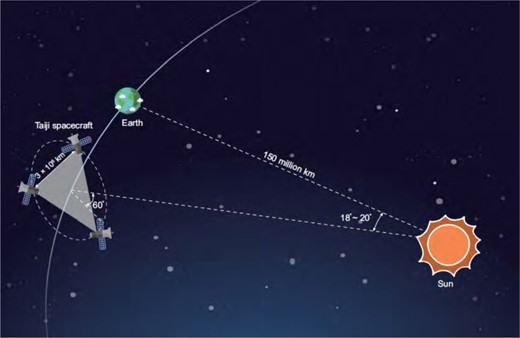
\includegraphics[width=0.86\textwidth]{figures/PTEP2021_Taiji_fig1.jpeg}
\caption{太极（Taiji）空间引力波探测器星座示意图。太极三颗航天器构成臂长约 $3\times10^6\,\mathrm{km}$ 的近似等边三角形星座，星座中心沿日心轨道运行，并与地球保持约 $18^\circ$--$20^\circ$ 的角距离。该轨道构型使太极在毫赫兹频段获得长期稳定的空间干涉基线，也为与 LISA 等日心轨道任务开展联合观测提供了方向图互补性。图片引自 Luo 等~\cite{Luo2021Taiji_PTEP} 的 Figure 1。}
\label{fig:taiji_constellation}
\end{figure}

\section{全局拟合：空间引力波数据分析的核心难题}

全局拟合（Global Fit）是空间引力波数据分析的重要目标：同时对探测器数据中大量重叠信号源进行联合参数估计。其必要性来自信号的相互耦合——单个信号的参数估计会受到其他信号的干扰，联合分析是控制这类系统误差的关键途径。

全局拟合的计算挑战极为严峻。参数空间维度可达到 $10^5$--$10^7$ 量级，具体取决于可分辨银河系双星数量、是否显式建模弱源混淆背景、EMRI数量以及SGWB参数化方式。传统 MCMC 方法难以直接用于如此高维且强相关的参数空间，即便采用先进的嵌套采样算法，完整全局拟合也可能超出现实任务预算。

当前最接近实用的全局拟合方案多采用迭代减除或分块联合拟合策略：首先识别并减除最强或最易分离的信号，然后在残差数据上继续搜索和更新其他源，如此迭代直至主要可分辨信号被提取。这一策略的关键假设是信号强度和频域结构存在可利用的层级，以及每步减除的精度足够高以避免残差污染后续步骤。AI 方法在每个迭代步骤中的快速搜索和参数估计能力，是使这一策略在实践中可行的重要技术支撑。

人工智能方法在全局拟合中的角色是分层的：快速搜索方法（第5章）提供强信号的初始定位，SBI 方法（第6章）对各类源进行快速参数估计，去噪方法（第7章）处理非稳态噪声，最终由全局拟合框架整合这些中间结果。这一分层架构使人工智能方法不再只是单点工具，而成为空间任务数据处理基础设施的一部分。

\subsection{全局拟合的数学框架}

全局拟合的核心是对联合后验分布的估计。设探测器数据为 $d$，探测器中同时存在 $K$ 个信号源，第 $k$ 个信号源的参数向量为 $\theta_k$，则全局后验分布为：
\begin{equation}
p(\{\theta_k\}_{k=1}^K | d) \propto p(d|\{\theta_k\}) \prod_{k=1}^K p(\theta_k),
\end{equation}
其中 $p(\theta_k)$ 是各信号源参数的先验分布，$p(d|\{\theta_k\})$ 是联合似然函数。由于大量信号在频域叠加，联合似然函数通常不能简单分解为各信号似然的乘积——许多频率bin同时携带多个信号的贡献，使得对单一信号源的分析需要同时考虑其他强信号、混淆背景和噪声模型。

在高斯噪声假设下，联合似然函数的对数为：
\begin{equation}
\ln p(d|\{\theta_k\}) = -\frac{1}{2} \left\langle d - \sum_k h(\theta_k) \,\bigg|\, d - \sum_k h(\theta_k) \right\rangle,
\end{equation}
其中 $h(\theta_k)$ 是第 $k$ 个信号源在探测器中产生的应变，内积 $\langle \cdot | \cdot \rangle$ 按噪声功率谱密度加权。由于参数总维度 $\sum_k \dim(\theta_k)$ 可达 $10^5$--$10^7$ 量级，直接对联合后验进行逐点采样在当前计算预算下难以承担。

当前代表性的全局拟合实现多采用分块-迭代策略：将 $K$ 个信号源按类型分组（MBHB组、EMRI组、银河系双星组、背景组），在每个迭代步骤中固定或边缘化其他组的近似参数，对当前组进行贝叶斯推断，然后更新当前组的参数后继续迭代。这一策略将高维联合优化分解为一系列低维子问题，但代价是收敛速度较慢且依赖良好的初始化。

GLASS、BALROG 等框架是当前空间引力波全局拟合研究中的代表性实现。它们通常采用迭代残差减除、贝叶斯模型选择、多模态采样或分块优化等技术，在LISA数据挑战（LDC）等模拟数据上验证了处理复杂多源场景的可行性。不同框架在计算效率、模型完备性和后验精度之间有不同取舍，距离完整任务规模的在线全局拟合仍需进一步发展。

\subsection{AI在全局拟合中的分层架构}

\begin{figure}[htbp]
\centering
\resizebox{0.96\textwidth}{!}{%
\begin{tikzpicture}[
  font=\small,
  band/.style={draw, rounded corners=5pt, minimum width=12.2cm, minimum height=1.85cm,
               align=left, inner sep=5pt},
  l0/.style={band, fill=gray!10, draw=gray!50},
  l1/.style={band, fill=blue!7, draw=blue!45},
  l2/.style={band, fill=green!7, draw=green!45},
  l3/.style={band, fill=orange!8, draw=orange!55},
  method/.style={draw, rounded corners=2pt, minimum width=3.35cm, minimum height=0.68cm,
                 text centered, align=center, font=\scriptsize, fill=white},
  layerlabel/.style={font=\small, align=left},
  arr/.style={-Stealth, thick, gray!60},
]
\node[l0] (lay0) at (0,0) {};
\node[l1, below=4mm of lay0] (lay1) {};
\node[l2, below=4mm of lay1] (lay2) {};
\node[l3, below=4mm of lay2] (lay3) {};

\node[layerlabel, anchor=north west] at ([xshift=4mm,yshift=-3mm]lay0.north west)
  {第零层：快速搜索层（毫秒--秒级）};
\node[layerlabel, anchor=north west] at ([xshift=4mm,yshift=-3mm]lay1.north west)
  {第一层：参数估计层（秒--分钟级）};
\node[layerlabel, anchor=north west] at ([xshift=4mm,yshift=-3mm]lay2.north west)
  {第二层：全局融合层（天--周级）};
\node[layerlabel, anchor=north west] at ([xshift=4mm,yshift=-3mm]lay3.north west)
  {第三层：验证层（PP图、覆盖率检验）};

\node[method] (m01) at ([xshift=-3.9cm,yshift=-0.45cm]lay0.center) {MBHB快速搜索\\Ruan等，秒级};
\node[method] (m02) at ([yshift=-0.45cm]lay0.center) {EMRI两层CNN\\Yun等，分钟级};
\node[method] (m03) at ([xshift=3.9cm,yshift=-0.45cm]lay0.center) {全源统一检测\\Zhao等，模拟};

\node[method] (m11) at ([xshift=-3.9cm,yshift=-0.45cm]lay1.center) {归一化流/CNF\\MBHB（秒级）};
\node[method] (m12) at ([yshift=-0.45cm]lay1.center) {CNF-EMRI\\17维（分钟级）};
\node[method] (m13) at ([xshift=3.9cm,yshift=-0.45cm]lay1.center) {批量参数估计\\银河系双星（ms级）};

\node[method, minimum width=4.2cm] (m21) at ([xshift=-2.2cm,yshift=-0.45cm]lay2.center)
  {全局拟合优化器\\分块联合推断};
\node[method, minimum width=4.2cm] (m22) at ([xshift=2.2cm,yshift=-0.45cm]lay2.center)
  {残差信号更新\\迭代减除与回填};

\node[method, minimum width=4.2cm] (m31) at ([xshift=-2.2cm,yshift=-0.45cm]lay3.center)
  {统计校准\\PP图与覆盖率};
\node[method, minimum width=4.2cm] (m32) at ([xshift=2.2cm,yshift=-0.45cm]lay3.center)
  {物理审查\\异常事件复核};

\draw[arr] (lay0.south) -- (lay1.north);
\draw[arr] (lay1.south) -- (lay2.north);
\draw[arr] (lay2.south) -- (lay3.north);
\end{tikzpicture}}
\caption{空间引力波数据分析的分层人工智能架构示意图。第零层（快速搜索）在秒至分钟级内完成数据流的信号普查，提供参数空间初始定位；第一层（参数估计）对各类源进行快速近似或精细参数估计；第二层（全局融合）以第一层结果为初始值运行全局拟合；第三层（验证）通过PP图和覆盖率检验等工具评估结果的统计可靠性。图中时间尺度为基于现有代表性研究的任务级估计，并非完整任务流水线的正式性能指标；相关方法背景依据文献~\cite{ruan2023mbhb,zhao2023spacegw,liang2026sbireview,wang2024challenges,du2026taiji}综合改绘。}
\label{fig:global_fit_layers}
\end{figure}

当前主流的解决思路是构建分层的人工智能辅助架构，将全局拟合分解为多个计算上可行的子问题，由不同的人工智能组件分别处理，最后通过全局优化器整合结果。

第零层（快速搜索层）负责对数据中各类信号的初步普查。Ruan等的MBHB快速搜索在数秒内完成对一年模拟数据的扫描；Yun等的EMRI两层CNN探测器在分钟级时间内完成对EMRI候选体的普查；Zhao等的全源统一检测网络在所采用的模拟设置中同时标记多类信号候选。这一层的输出是各类信号候选体的初步位置（在参数空间中的粗定位），为后续精确推断提供初始化信息，减少从宽先验出发的低效采样。

第一层（参数估计层）对各类源的参数进行快速近似或精细估计。归一化流和CNF方法可对MBHB候选体给出约15维参数后验（秒至分钟级）；CNF方法对EMRI候选体探索17维参数后验估计；简单参数化方法可对银河系双星给出低维参数估计（毫秒级，适应大规模批量处理）。这一层的输出是各信号源的近似参数后验分布，作为第二层全局融合的输入。

第二层（全局融合层）将第一层结果作为初始值或提议分布，运行全局拟合算法。由于第一层已经提供了较好的初始参数估计，全局拟合所需的迭代次数有望减少，计算代价可能从月级量级压缩至天至周级量级。全局融合层的输出是联合后验分布的近似，用于计算主要可分辨信号源参数的最终估计和不确定度。

第三层（验证层）对第二层输出进行统计一致性检验：PP图检验SBI输出的后验分布是否经过校准，覆盖率检验确认可信区间的统计意义，并对异常事件（如显著偏离GR预言的信号）开展专项分析。这一层的存在是全局拟合结果能够获得科学界信任的必要条件。

\subsection{迭代减除的误差积累与AI精度要求}

迭代减除策略的可行性依赖于每步减除的精度足够高，使得残差中的信号残留不会对后续步骤造成显著污染。量化分析这一要求，可以给出AI方法精度的硬性门槛。

设每步参数估计的系统误差为 $\epsilon$（定义为参数估计偏差与真值之比），则该步减除后，残差中保留的信号功率约为 $\epsilon^2$ 倍的原始信号功率。对于有 $N$ 个可分辨银河系双星的迭代减除，若每步精度 $\epsilon$，则经过 $N$ 步后，残差中所有双星的信号残留叠加的总功率约为 $N\epsilon^2$ 倍的平均信号功率。当 $N\epsilon^2 \sim 1$ 时，残差噪声地板与单个双星信号相当，后续的EMRI等弱信号分析将受到严重干扰。

对于 $N\sim10^4$（可分辨银河系双星数量的保守估计），这一简单估算给出 $\epsilon < 1/\sqrt{N} \approx 0.01$ 的量级要求，即每步参数估计的系统误差需要接近百分之一量级。真实管道中的要求会随信号强度分布、频率重叠程度和误差相关性而变化，但这一估算说明：SBI方法的系统误差（由训练集偏差、网络容量限制等引起）需要被严格校准，才可能支撑迭代减除的稳定运行。进一步压缩并量化系统误差，是全局拟合从概念验证走向实际应用的关键技术挑战。

\section{主要波源类型的人工智能分析方法}

\subsection{大质量双黑洞：从快速搜索到精确参数估计}

MBHB 并合是空间引力波探测器最强的信号源，其低延迟探测对多信使天文学至关重要。Ruan 等人~\cite{ruan2023mbhb} 开发的深度学习快速搜索方法能够在\textbf{数秒量级}处理一年的 LISA 模拟数据；在所采用的测试集中，该方法识别了注入的 MBHB 并合事件，并未报告误报。需要强调的是，这一结果来自特定模拟数据集和评估条件，真实任务中的误报率还需结合噪声非平稳性、数据质量标记和统计显著性评估进一步验证。即便如此，其计算效率的量级优势仍使其成为全局拟合分析的有力初始化工具。

在参数估计层面，Du、Liang、Wang 等人~\cite{du2024normflow} 将归一化流方法应用于太极任务的 MBHB 参数估计，处理了太极特有的时变响应函数和混淆噪声背景，实现比传统方法快几个数量级的推断速度。Liang 等人~\cite{liang2024cnfmbhb} 进一步引入连续归一化流（CNF）和流匹配技术，在精度和速度上均有提升。Sun 等人~\cite{sun2025cvae} 的混合推断方案（CVAE + 贝叶斯采样）在三探测器（太极 + LISA + 天琴）联合观测场景下，将采样时间压缩至原来的 14.0\%，同时维持贝叶斯精度。

在具体方法实现上，Ruan等的深度学习快速搜索使用ResNet作为骨干网络，输入为TDI（时间延迟干涉）AET数据通道的时频表示。网络在LDC Radler数据集（包含若干注入MBHB事件的1年模拟数据）上训练和测试，在该设置中成功识别注入事件且未报告误报，单次处理时间约为秒级。相比于传统模板搜索方法，这一计算优势使得MBHB的近实时监测成为可能，对于捕捉电磁对应体具有重要意义。

Du等的归一化流参数估计在对数总质量、质量比、自旋、天空位置、距离、倾角、极化角和并合时刻等约15个参数上给出后验估计。特别值得注意的是，太极的时变响应函数会使天空位置后验呈现多模态结构（一年运动过程中，探测器对同一天空位置的敏感性随时间变化，导致存在多个似然极大值），而归一化流方法的生成建模能力有助于处理这种多模态性。Liang等的CNF方法（基于流匹配技术）进一步改善了多模态后验的建模，在天空位置参数的覆盖率检验中表现出较好校准性。

\subsection{极端质量比旋入：高维参数空间的突破}

EMRI 是空间引力波数据分析中最困难的问题之一。其 17 维参数空间、强参数简并（多极大值似然函数）、以及较高的波形计算代价，使直接传统 MCMC 方法在现实计算预算下面临严峻挑战。

Yun 等人~\cite{yun2024emri} 提出的两层 CNN 方法在 SNR 50--100 的模拟范围内实现了 96.9\% 的 EMRI 探测真正率，并在测试设置中给出超大质量黑洞质量和自旋的高精度估计，为后续参数估计压缩搜索空间。Liang 等人~\cite{liang2024cnfemri} 将连续归一化流应用于 EMRI 参数估计，在 17 维参数空间中展示了比传统采样快几个数量级、且在模拟测试中通过校准检验的推断能力，是机器学习方法进入这一高难度问题的重要进展。

Yun等的两层CNN方法针对EMRI探测的特殊困难进行了专门设计。EMRI信号在频域表现为密集的谐波梳状结构，每个谐波的频率随时间缓慢演化（频率漂移量级取决于源参数），与银河系双星的近单频信号有本质区别。第一层CNN输入为TDI AET通道数据的时频谱图，通过多尺度卷积捕获EMRI谐波的特征模式，输出为“EMRI候选”或“非EMRI”的二分类决策。第二层CNN对第一层确认的候选体进行精细特征提取，直接估计超大质量黑洞的质量和自旋——这两个参数决定了Kerr时空的主要几何特征，是EMRI轨道频率结构的主要决定因素。通过预先估计这两个参数，后续精确参数估计的搜索空间可从17维压缩至约15维，从而降低计算代价。

Liang等的CNF-EMRI工作是机器学习方法在空间引力波数据分析中值得重视的成果，其意义超越了单纯的技术加速。在方法论层面，它表明SBI方法有能力处理引力波数据分析中高度困难的参数估计问题——17维强简并参数空间中的多极大值后验分布——而传统MCMC方法对此类问题的收敛时间可能达到多年量级。在科学意义层面，更高效的EMRI参数估计将支持太极/LISA实现其旗舰科学目标——对超大质量黑洞周围Kerr时空的精密测绘，并为广义相对论和黑洞无毛定理的强场检验提供关键数据分析工具。在方法论推广层面，CNF在EMRI这一高难度问题上的成功，说明SBI方法有潜力扩展到更广泛的高维强简并推断场景，但其适用范围仍需要在更多物理模型、噪声条件和先验设定下系统检验。

Liang等的CNF-EMRI方法是当前EMRI参数估计中具有代表性的机器学习实现。训练集由FastEMRIWaveforms（FEW）生成的约50万条EMRI波形（覆盖17维参数空间）组成，FEW通过快速波形生成技术显著降低了单条波形的生成时间。网络架构为条件归一化流，以TDI AET三通道的频域表示为条件输入，输出17维参数的联合后验分布。在独立测试集上，17个参数的PP图在统计误差内通过一致性检验，表明后验分布在该模拟设置下具有良好的校准性。推断时间达到秒级或亚秒级（GPU加速），较传统采样方法实现了数量级加速。

\subsection{全源类型统一检测}

Zhao 等人~\cite{zhao2023spacegw} 提出的多阶段自注意力深度神经网络，在所采用的模拟设置下探索了对多类空间引力波源（银河系双星、MBHB、EMRI、随机背景）的统一检测与提取；在 SNR = 50、误报率 1\% 的条件下，各类源检测率达到较高水平。这一统一框架的意义在于：它减少了为每类源单独开发和维护专用算法的工程复杂性，为全局拟合管道提供了统一信号检测前端的可能方案。

多阶段自注意力架构的核心设计思想是：不同类型的引力波信号具有不同的时频特征模式，但都可以在足够宽广的特征空间中被统一表示。第一阶段使用多尺度卷积提取局部时频特征（适合捕获银河系双星的单频模式和EMRI的谐波梳结构）；第二阶段使用Transformer自注意力机制捕获长程时序相关性（适合追踪MBHB长达数月的旋入演化）；第三阶段使用多头输出头（multi-head output）同时对四类源给出检测决策。

在SNR = 50的模拟条件下，MBHB、EMRI和双白矮星等源的检测率均达到较高水平，随机背景振幅估计也表现出一定精度；在SNR较低的样本上，检测率有所下降但仍保持可用水平。这一统一检测框架在实际全局拟合管道中可以作为数据预处理的第一道关口，快速筛选出各类信号候选体，为后续专用参数估计方法提供输入。其真实任务性能仍需在更复杂噪声、源重叠和不完整训练分布下进一步验证。

\section{非稳态噪声：从理想模拟到真实管道}

早期空间引力波数据分析研究大多基于理想化的平稳高斯噪声假设。然而，真实的空间探测器在运行中不可避免地产生各种非稳态噪声，这些噪声在地面测试中难以完全预测和模拟。

Xu 等人~\cite{xu2024nonstationarty} 系统研究了三类可预见的非稳态噪声：数据间隙（例行维护或意外中断导致的数据缺失）、暂态噪声（仪器或环境扰动产生的短时高幅度脉冲）、以及时变噪声自相关（噪声功率谱密度的缓慢漂移）。针对这三类噪声及其混合情形，该工作开发的深度学习模型在保持理想场景性能的同时，展示了显著的非稳态适应性。

Du 等人~\cite{du2026taiji} 的受邀综述进一步指出，从理想化的 LISA 数据挑战（LDC）场景到太极真实探测管道，数据分析面临的挑战远比预期复杂：高保真探测器响应仿真、轨道动力学效应、时间延迟干涉（TDI）的精确实现，以及多种噪声源的联合建模，都需要系统性的方法论突破。

\subsection{太极的噪声模型与TDI原理}

太极的噪声模型由三类主要成分构成，各自在不同频段主导探测器的灵敏度极限。

第一类是加速度噪声（acceleration noise），来源于残余气体分子碰撞、宇宙线打击、热辐射压力涨落等对检验质量的随机力扰动。其功率谱密度为：
\begin{equation}
S_a(f) = \left(3\times10^{-15}\right)^2 \left[1 + \left(\frac{4\times10^{-4}\,\mathrm{Hz}}{f}\right)^2\right] \,\mathrm{m^2\,s^{-4}\,Hz^{-1}},
\end{equation}
在低频段（$f < 4\times10^{-4}$ Hz）随 $f^{-2}$ 增长，是低频灵敏度的主要限制因素。

第二类是光学路程噪声（optical path noise），来源于激光相位噪声残余、光子散粒噪声、望远镜热形变等。其功率谱密度约为：
\begin{equation}
S_\mathrm{opt}(f) \approx \left(1\times10^{-12}\right)^2 \,\mathrm{m^2\,Hz^{-1}},
\end{equation}
在高频段（$f > 10^{-2}$ Hz）近似为白噪声，是高频灵敏度的主要限制因素。

第三类是激光频率噪声，其量级约为 $10^9$ Hz/$\sqrt{\mathrm{Hz}}$，比引力波信号（等效位移噪声约 $10^{-12}$ m/$\sqrt{\mathrm{Hz}}$）大约12个量级。如此巨大的激光频率噪声必须通过时间延迟干涉（TDI）技术消除，才能使引力波信号从噪声中显现。

TDI的工作原理是通过延迟各臂的激光信号并进行线性组合，在代数上抑制激光频率噪声。以最简单的Michelson X通道为例，其构造可示意为：
\begin{equation}
X = (D_{31}D_{13} - 1)h_1 + (D_{13} - D_{31})h_2 + \cdots,
\end{equation}
其中 $D_{ij}$ 表示沿臂 $ij$ 方向的时间延迟算符，$h_i$ 表示第 $i$ 颗卫星上的激光相位测量。当臂长近似恒定时，激光频率噪声可在一阶TDI组合中高度相消；当臂长随时间变化时，需要使用第二代TDI（TDI 2.0）处理时变臂长效应。实际数据处理中，亚采样延迟通过Lagrange插值或sinc插值实现，插值精度直接影响TDI的激光噪声抑制效果。

TDI生成的A、E、T三个正交通道（由X、Y、Z通道的线性组合构成）具有不同的方向图响应：A和E通道对引力波信号敏感，T通道在低频段对引力波不敏感，可用于监测仪器噪声。这三个通道的联合分析是空间引力波数据处理的标准输入格式。

\subsection{三类非稳态噪声的物理机制与影响}

数据间隙是空间引力波探测器运行中需要重点考虑的非稳态数据质量问题。其来源包括：例行维护操作（激光重新锁定、推进器点火调轨）、意外中断（宇宙线打击导致的仪器复位）、以及数据传输中断。典型的数据间隙持续时间可能从数秒到数小时不等，发生率需由实际任务运行状态和地面测控策略确定。

数据间隙对TDI的影响具有特殊性：由于TDI利用延迟相消，单臂数据间隙会通过延迟算符传播，导致TDI输出的多个时间点同时受影响。具体地，若某臂在时刻 $t_0$ 发生持续 $\Delta t$ 的数据间隙，则TDI X通道在 $t_0$、$t_0 + L/c$、$t_0 + 2L/c$ 等多个时刻均受到影响（$L$ 为臂长，$c$ 为光速），形成“扩散”的噪声超出。这一传播效应使得数据间隙的影响范围远大于间隙本身的持续时间，对后续信号分析造成更广泛的干扰。

暂态噪声（glitch）在太空环境中的来源可能包括宇宙线打击、激光锁定失调、推进器动作和热控扰动等。高能粒子穿过检验质量时，可能通过电荷沉积或动量传递引发短时扰动；太阳活动周期也会影响带电粒子环境。由于具体发生率和振幅分布依赖探测器设计、轨道环境和在轨控制策略，相关模型应在技术验证任务和主任务早期数据中持续标定。

时变噪声自相关（time-varying noise PSD）可能来源于探测器热环境、激光链路状态、检验质量带电状态和太阳活动等因素的缓慢变化。卫星热控系统虽然维持激光器和光学平台的温度稳定，但微小温度涨落仍可能导致激光功率、光学路程和加速度噪声的缓慢漂移。此外，太阳耀斑、日冕物质抛射等事件会影响卫星热环境和带电粒子环境，导致噪声特性的突变。

Xu等鲁棒模型的关键设计是在训练集中系统性地引入各类非稳态噪声的模拟样本，使网络学习对噪声类型变化较不敏感的表示。在理想噪声、数据间隙、glitch以及混合非稳态噪声等测试情形中，鲁棒模型相对于只在理想噪声上训练的基线表现出更稳定的重叠度。这一结果表明，通过训练集的系统性扩充，可以在受控模拟条件下显著提升模型对复杂运行条件的适应能力；但其在真实在轨噪声中的表现仍需要后续数据验证。

\section{高保真仿真与现实探测管道的构建}

空间引力波数据分析算法的开发和验证，依赖于高保真的模拟数据。Du 等人~\cite{du2026taiji} 的综述系统梳理了太极高保真仿真的关键要素：

\textbf{探测器响应仿真}：太极星座的轨道运动导致探测器响应函数随时间变化（一年周期），需要精确的轨道动力学模型和时间延迟干涉（TDI）实现。早期工作（Du、Liang、Wang 等~\cite{du2024normflow}）已揭示这一时变响应在参数估计中引入的额外多模态结构。

\textbf{波源模型的完备性}：高保真仿真需要覆盖主要预期波源类型，包括银河系双星种群模型、MBHB 波形、EMRI 的 Kerr 时空轨道演化，以及各类随机背景的功率谱模型。

\textbf{噪声模型的真实性}：从理想高斯噪声到包含非稳态成分的真实噪声，是算法从实验室走向实际应用的关键一步。Xu 等人~\cite{xu2024nonstationarty} 的工作为这一过渡提供了方法论基础。

\textbf{多任务协同}：太极、LISA、天琴三个任务若能形成重叠观测，将有望提升参数估计精度（Sun 等~\cite{sun2025cvae} 在三探测器场景下的验证）和天空定位能力。跨任务算法的共享与优化，是降低整体研发成本的重要方向。

空间引力波数据分析的最终目标，是构建一个能够在任务运行期间持续、自动、可靠地处理海量数据的完整管道。这一管道需要将本书前述各章的方法——信号识别（第5章）、参数估计（第6章）、去噪（第7章）、算法自动发现（第8章）、物理-数据融合（第9章）——有机整合，形成一个既高效又可靠的科学数据处理系统。AI 方法在这一系统中不只是单点性能优化，而是提高完整管道计算可行性的重要使能技术。

高保真仿真基础设施的建设不仅服务于算法开发和测试，还在科学验证中发挥关键作用。太极任务发射后，高保真仿真器可用于校准在轨探测到的信号：通过将观测数据与高保真模拟预测对比，可以发现系统误差的来源（如TDI实现的不完善、轨道动力学模型的偏差），并指导数据分析算法的在线更新。LDC（LISA数据挑战）的历史演进已经展示了这一“模拟→算法开发→模拟升级→算法改进”迭代循环的价值：从早期较理想化的数据集，到包含多源叠加和更真实探测器响应的复杂模拟，挑战赛不断暴露算法在新条件下的不足，并推动全局拟合、MBHB搜索和AI方法的发展。太极高保真仿真平台的建设，是这一良性循环在中国主导的空间引力波任务中的延续。其深层意义在于：每一轮仿真升级不仅提高数据真实性，还通过暴露算法缺口来驱动方法创新，从而在任务发射前积累更充分的方法论储备并降低在轨数据分析风险。

\subsection{EMRI波形生成的数值方法与快速近似}

EMRI波形生成是空间引力波数据分析中计算代价最高的环节之一，也是制约EMRI参数估计可行性的关键瓶颈。精确的EMRI波形需要求解Kerr时空中的Teukolsky方程，这是一个描述Kerr背景上引力扰动的偏微分方程，其数值求解需要处理复杂的边界条件和大量的谐波模式。

EMRI轨道演化基于Kerr时空中的测地线方程，考虑引力自力（gravitational self-force）对轨道的反作用效应。引力自力是小质量天体在大质量黑洞引力场中运动时，自身引力场对自身轨道的反作用，其效应导致轨道能量和角动量的缓慢耗散，驱动轨道向内螺旋并最终并合。精确计算引力自力需要求解一阶（甚至二阶）引力自力方程，这在数值上极为昂贵，目前仅对特定轨道构型（如圆形赤道轨道）有完整的数值结果。

FastEMRIWaveforms（FEW）框架通过快速谐波求和、插值和GPU加速等技术，将单次EMRI波形生成时间从传统实现的分钟级显著压缩到秒级甚至更短。FEW的核心思想是利用EMRI波形的多谐波结构，将模式振幅、相位和轨道演化中的昂贵部分预计算或高效近似；在给定轨道参数后，通过查表、插值和快速叠加得到波形。这一方法在速度和精度之间取得了实用折中，是EMRI参数估计和SBI训练的重要使能技术。

\subsection{LISA数据挑战的历史演进与AI方法的崛起}

LISA数据挑战（LDC）是推动空间引力波数据分析方法发展的重要平台，其历史演进反映了数据分析问题从单源、理想噪声逐步走向多源叠加和更高保真仿真的过程。

早期的 Mock LISA Data Challenges 主要围绕单源或少量源的检测与参数估计展开，验证了贝叶斯采样、MCMC、嵌套采样和匹配滤波类方法在MBHB、银河系双星和EMRI问题上的可行性，同时也暴露了计算代价和源混叠处理的困难。随着挑战数据集逐步纳入银河系双星混淆背景、多个源类和更真实的探测器响应，全局拟合问题逐渐成为核心议题。

近年的LDC数据集（如Radler、Sangria等）进一步提高了源叠加、探测器响应和噪声模型的复杂度，为机器学习方法提供了更接近任务需求的验证环境。Ruan等的深度学习方法在Radler类MBHB快速搜索任务中展示了秒级扫描一年模拟数据的能力，说明AI方法可以在空间引力波低延迟搜索中发挥重要作用。需要强调的是，这些结果仍属于模拟数据挑战中的性能验证，能否直接迁移到真实任务管道，还取决于噪声模型、信号分布、数据质量标记和统计显著性评估的进一步完善。

总体而言，LDC的价值不在于给出某一类方法的最终胜负，而在于提供可复现的共同基准，使传统贝叶斯方法、全局拟合框架和AI方法能够在同一数据条件下接受检验。未来空间引力波数据分析很可能形成“AI快速搜索与初始化 + 贝叶斯/全局拟合精确验证”的协同格局，而不是由单一方法完全主导。

\section{数据分析管道的系统工程挑战}

从单一方法的研究原型到能够在任务运行期间可靠运行的完整数据分析管道，需要跨越一系列系统工程层面的挑战。这些挑战不属于算法本身，而属于将算法集成为可运行系统的工程实践。

\subsection{实时性与低延迟要求}

大质量双黑洞并合的多信使天文学对数据分析提出了严格的低延迟要求。若存在可观测电磁对应体，从并合发生到可观测亮度峰值可能只有数小时至数天的时间窗口。这意味着数据分析系统需要尽可能在并合发生后数分钟至数小时内完成初步探测和天空定位，才能有效指导后续的电磁观测。

当前地面引力波数据分析系统（如 GstLAL）已能实现分钟级的低延迟预警。对于空间探测器，由于信号持续时间更长（旋近阶段数月至数年），低延迟分析的难度不在于快速处理单次数据，而在于持续追踪信号演化并动态更新并合时刻预测。Xu 等人~\cite{xu2024denoising} 的旋近去噪框架提供了实现这一目标的方法论基础，但将其集成为连续运行的实时系统仍有大量工程工作。

\subsection{模型更新与在线学习}

空间引力波探测器的运行周期预计长达5至10年。在如此漫长的运行期间，探测器的仪器特性（噪声功率谱、仪器响应函数）将随时间缓慢变化，而科学目标的优先级也可能随早期观测结果的发现而调整。这要求数据分析系统能够随时间更新模型参数，而不是依赖在运行开始前训练的固定模型。

机器学习方法在此面临特有挑战：重新训练大型神经网络模型需要大量计算资源，而在线增量学习（online incremental learning）在保持旧知识的同时学习新数据（即避免“灾难性遗忘”）是机器学习领域尚未完全解决的难题。灾难性遗忘（catastrophic forgetting）是指神经网络在学习新任务时，由于权重更新覆盖了旧任务的知识表示，导致旧任务性能急剧下降的现象。在太极任务中，探测器噪声特性随时间变化，需要持续更新模型以适应新的噪声条件，而不能遗忘在早期数据上学到的信号特征。

弹性权重固化（Elastic Weight Consolidation，EWC）是缓解灾难性遗忘的经典方法，其核心思想是在损失函数中加入正则化项，惩罚对旧任务重要参数的大幅修改。具体地，EWC在学习新任务时，通过Fisher信息矩阵估计每个参数对旧任务的重要性，并对重要参数施加弹性约束，使其在新任务学习过程中保持相对稳定。课程学习（curriculum learning）按照难度逐步引入新样本，也有助于稳健地更新模型。Evo-MCTS框架提供了另一种思路：不更新预训练神经网络的权重，而是在算法层面持续进化，适应新的噪声条件——这一方法天然避免了灾难性遗忘问题，因为进化搜索不依赖于固定的神经网络权重。

\subsection{验证、确认与科学可信度}

引力波数据分析系统的科学输出（引力波事件目录、参数估计结果）将成为后续科学研究的基础数据。这要求分析管道能够提供可靠的不确定度量化——不仅是统计不确定度（后验分布的宽度），还包括系统不确定度（模型误差、噪声模型偏差、算法近似误差）。

对于机器学习方法，系统不确定度的评估尤为困难。神经网络在训练分布内通常过度自信（confidence calibration 问题），而在训练分布外则可能给出毫无意义的置信度。建立引力波 AI 方法的系统不确定度量化框架，是其从研究工具走向科学生产系统的必要条件，也是当前领域最活跃的研究方向之一。

PP图（probability-probability plot）是SBI方法统计一致性验证的核心工具。对于一个经过正确校准的后验估计器，若从先验分布中采样真实参数 $\theta^*$，生成对应的模拟数据 $d$，然后用SBI估计后验 $p(\theta|d)$，则 $\theta^*$ 在后验分布中的分位数应服从均匀分布。PP图通过绘制分位数的经验累积分布函数与理想均匀分布的对比，直观展示后验估计的校准质量。偏离对角线表明后验估计存在系统偏差（过度自信或过度保守），需要通过后处理校准（如等分回归）加以修正。

\subsection{容错与鲁棒运行}

空间引力波探测器在太空运行期间很可能遇到各种异常情况：数据间隙（卫星维护、激光锁定失调）、仪器噪声突变、宇宙线打击导致的暂态噪声等。数据分析系统需要对这些异常情况具备鲁棒性，不仅不被异常数据误导，还能在异常恢复后快速重新同步分析状态。

Xu 等人~\cite{xu2024nonstationarty} 对三类非稳态噪声的系统研究，是为空间引力波数据分析管道建立鲁棒性设计规范的重要起点。未来的完整管道还需要在此基础上，开发针对其他可能异常情况的处理策略，以及异常检测和恢复的自动化机制。异常检测本身也可以借助AI方法：通过训练一个专门识别各类仪器异常（数据间隙、glitch、噪声突变）的分类器，在数据进入主分析管道之前进行预筛选，将异常数据段标记并路由到专用处理模块，从而保护主分析管道不受异常数据的干扰。

在系统工程挑战中，“科学与工程的协作模式”是一个往往被忽视但至关重要的维度。引力波数据分析软件既是科学工具（产出科学结论），也是工程系统（需要持续运行、维护和更新）。在LIGO-Virgo时代，这一张力通过大型国际合作组织（LSC，LIGO Scientific Collaboration）来协调：科学家设计分析方法，工程师实现并维护计算基础设施，软件工作委员会（Software Working Groups）协调两者的衔接。对于太极任务，建立类似的科学-工程协作机制是AI驱动数据分析管道能够从实验室走向生产系统的制度保障。特别是，AI模型的版本管理（记录哪个模型处理了哪段数据）、模型更新的回溯验证（新模型是否与旧模型给出一致的历史结果）、以及算法文档的完备性（使未来研究者能够重现当前的分析结果），都需要在制度层面建立规范，这是人工智能方法在严肃科学中负责任应用的基本要求。从LIGO的经验来看，科学-工程协作机制的建立本身也是一个迭代过程：早期的LIGO数据分析软件以科学家的原型代码为主，工程化水平有限；随着探测事件的积累和数据规模的增长，LIGO逐步建立了完善的软件工程规范，包括代码审查流程、持续集成测试、以及详细的版本控制记录。太极任务可以从LIGO的这一历史中汲取宝贵经验，从任务立项阶段便开始规划科学-工程协作框架，避免在任务运行中期因制度缺失而引发的数据质量危机。

\begin{table}[htbp]
\centering
\caption{太极数据分析管道各层次的关键挑战与 AI 解决方案}
\label{tab:taiji_pipeline}
\small
\begin{tabular}{lll}
\hline
\textbf{管道层次} & \textbf{核心挑战} & \textbf{AI 解决方案} \\
\hline
信号检测 & 数百万信号同时叠加 & 多阶段自注意力网络（§5.4）\\
         & 计算实时性要求 & Evo-MCTS 自动优化管道（§8.3）\\
\hline
参数估计 & EMRI 17维强简并 & CNF 流匹配（§6.4）\\
         & MBHB 时变响应函数 & 归一化流+变换映射（§6.3）\\
         & 三探测器联合推断 & CVAE 混合推断（§6.5）\\
\hline
信号去噪 & 30天旋近低信噪比 & 深度去噪+并合时刻预测（§7.4）\\
         & 数据间隙/暂态噪声 & 鲁棒深度学习模型（§7.5）\\
\hline
全局拟合 & $10^5$--$10^7$ 量级参数空间 & 分层 AI 架构（§10.2）\\
         & 信号迭代减除 & 快速搜索初始化（§5.4.2）\\
\hline
系统工程 & 模型在线更新 & 进化搜索持续优化 \\
         & 不确定度量化 & SBI 统计一致性框架（§6.7）\\
\hline
\end{tabular}
\end{table}

从系统工程的视角审视，太极数据分析管道的构建是一项跨越十年、需要持续迭代的系统工程。与地面引力波探测器不同，太极在轨期间的数据特性（噪声谱、仪器响应）会随时间缓慢演化，算法必须具备在轨适应能力。这要求在管道设计之初就将“可更新性”作为核心设计原则：数据分析模块之间的接口应当标准化，使得任何模块（如信号搜索、参数估计、去噪）的算法升级不会破坏整体管道的稳定性；版本控制系统必须追踪每个数据段用哪个版本的算法处理，以确保科学结论的可复现性；在轨测试机制应利用已知的校准信号（如银河系内的已知双星系统）定期评估各模块的性能，及时发现并修正性能退化。这些系统工程要求看似琐碎，却是将实验室算法研究转化为可靠科学基础设施的关键步骤，也是引力波AI方法走向成熟的必要条件。

空间引力波探测器时代的数据分析，很可能逐步走向一种“人机协作的演化管道”模式：算法在任务运行中依据在轨数据和标准化评估结果持续更新，人类科学家定期审查和指导算法的更新方向，以确保科学目标的一致性和物理可解释性。这种模式相对于当前引力波数据分析中常见的“人工设计、定期更新”范式提出了新的制度、工程和方法论要求。太极团队的前期工作——从MF-CNN的物理先验嵌入，到CNF的EMRI参数估计，再到Evo-MCTS的算法搜索——可视为这种演化管道模式若干关键组件的原型验证，为太极任务的数据分析系统建设提供了方法论参考。

\section{太极数据分析挑战赛与开放科学}

引力波数据分析方法的快速进步，离不开标准化评估平台的驱动。LISA数据挑战赛（LISA Data Challenge，LDC）自2004年起持续举办，通过发布标准化模拟数据集，推动了全球范围内引力波数据分析算法的系统性比较与改进。面向太极任务的模拟数据挑战赛，可在这一经验基础上结合太极任务的具体技术参数和科学目标，构建中国空间引力波数据分析的评估体系。

\subsection{太极模拟数据挑战赛的设计}

太极模拟数据挑战赛（TDC）的设计可充分借鉴LISA数据挑战赛（LDC）的经验，同时针对太极任务的特殊性进行系统性改进。LDC历经多个版本迭代，从较理想化的单源或少量源检测，逐步演进至多源混合信号和全局拟合场景，积累了丰富的挑战赛设计经验。TDC在继承这一框架的基础上，需要将太极的轨道参数（臂长约300万公里、与地球保持约$20^\circ$角距离的日心轨道）、仪器噪声模型（位移噪声目标约$1\,\mathrm{pm}/\sqrt{\mathrm{Hz}}$、加速度噪声约$3\times10^{-15}\,\mathrm{m/s^2}/\sqrt{\mathrm{Hz}}$）以及科学目标优先级纳入数据集生成框架。

TDC模拟数据集的构成应覆盖太极的主要科学目标。大质量双黑洞并合（MBHB）信号可采用后牛顿波形、EOB波形或数值相对论代理模型生成，覆盖从阈值附近到高信噪比的宽泛范围。极端质量比旋入（EMRI）信号可采用快速EMRI波形生成器（FastEMRIWaveforms，FEW）~\cite{Chua2021FEW}等工具生成，包含轨道偏心率、轨道倾角、Kerr自旋参数等多维物理参数，信号持续时间从数月到数年不等。银河系双白矮星背景可由大规模双星种群叠加形成，其中一部分高频或高信噪比源可分辨，其余构成混淆噪声背景。仪器噪声模型则应从稳态高斯噪声基线逐步扩展到数据间隙、暂态噪声和时变PSD等非稳态成分，并结合技术验证任务和地面测试数据持续标定。

TDC的评估指标体系从三个维度综合评价参赛算法的性能。参数估计精度采用后验分布的覆盖率（coverage）和Jensen-Shannon散度（JSD）量化，要求在标准PP图检验中通过统计一致性验证。计算效率以单个事件的参数估计时间为基准，区分“实时分析”（$<$1小时）、“快速分析”（$<$1天）和“精确分析”（无时间限制）三个等级，对应不同的科学应用场景（多信使预警、常规目录发布、精密科学分析）。鲁棒性评估通过在训练集之外的参数区间（如极高红移MBHB、高偏心率EMRI）测试算法性能，量化算法对分布外样本的泛化能力。这一多维评估体系避免了单一指标优化导致的“过拟合评估”问题，更全面地反映算法在实际科学应用中的综合能力。

\subsection{开放科学基础设施}

太极数据分析的开放科学基础设施建设，是推动国际合作和算法快速迭代的关键支撑。在数据格式标准化方面，TDC类数据集宜尽量采用与LISA数据挑战赛兼容的数据格式，以HDF5为底层存储格式，统一定义时间序列数据的采样率、时间延迟干涉（TDI）通道命名（A、E、T）以及元数据结构（仪器参数、注入信号目录）。这一标准化设计可使为LDC开发的数据读取和预处理工具更容易迁移到太极模拟数据，降低国际参与者的技术门槛。

开源工具链的建设是TDC类开放科学基础设施的核心组成部分。LISA Tools生态系统提供了从轨道计算、TDI响应到噪声模拟的工具链；太极相关数据集可在此基础上开发针对太极轨道和噪声参数的适配模块，以提高与国际工具生态的互操作性。BBHx~\cite{Katz2020BBHx}是专为空间引力波探测器设计的GPU加速MBHB波形生成库，可显著降低大规模MBHB模拟数据集的生成成本。FastEMRIWaveforms（FEW）~\cite{Chua2021FEW}通过快速波形和代理模型加速EMRI波形计算，是构建EMRI模拟数据集的重要工具之一。

模拟数据集的公开发布宜遵循“分阶段开放”原则：挑战赛期间发布不含注入信号目录的盲测数据集，挑战赛结束后公开完整数据集（含真实参数）和评估代码；条件成熟时，可通过Zenodo等平台长期归档并分配DOI，以提高科学结论的可复现性。这类开放数据政策不仅有助于算法的公平比较，也可为后续研究者提供标准化的基准数据集，推动引力波数据分析方法论的累积性进步。

\subsection{挑战赛揭示的关键技术差距}

TDC类挑战赛的评估结果可系统性地揭示当前引力波数据分析方法与实际任务需求之间的关键技术差距，为未来研究方向提供优先级指引。

全局拟合的计算可行性是最核心的技术差距。当前代表性的全局拟合算法（如RJMCMC方法）在处理包含大量银河系双星、若干EMRI和偶发MBHB的混合数据集时，单次完整分析可能需要数周至数月的计算时间，难以满足低延迟分析需求。即便采用GPU加速和并行计算，基于传统采样的全局拟合方法在计算效率上仍面临数量级缺口。人工智能方法（特别是归一化流和扩散模型）在单源参数估计上已实现秒级推断，但如何将这一效率优势扩展到多源混合信号的联合分析，仍是尚未解决的核心问题。

EMRI信号的检测灵敏度是第二个关键差距。EMRI信号的低信噪比、长持续时间（数月至数年）和高维参数空间（17维）的组合，使其成为空间数据挑战中最具挑战性的信号类型之一。低SNR EMRI的检测率对波形模型、噪声背景和搜索策略高度敏感。提升低SNR EMRI的检测灵敏度，需要在波形模型精度（包含自力、偏心率和自旋效应）和检测统计量设计（利用EMRI信号的长时相干性）两个方向同时突破。

非稳态噪声对分析精度的影响是第三个关键差距，也是从理想化模拟到真实探测管道最难跨越的鸿沟。若数据挑战从稳态高斯噪声逐步引入数据间隙、暂态噪声毛刺和时变PSD，许多在理想条件下表现良好的算法都可能出现明显性能退化。因而，空间任务需要在噪声建模（非稳态噪声的实时估计与减除）和算法设计（对噪声非稳态性的显式建模）两个层面进行系统性改进。

\subsection{国际合作与竞争格局}

LISA、太极和天琴三个空间引力波探测任务在数据分析方法上既存在激烈竞争，也有深度合作的内在需求，形成了独特的国际合作与竞争格局。

在方法互补性方面，三个任务的数据分析团队在技术路线上各有侧重，形成了有益的多样性。LISA数据分析团队（主要来自欧洲和美国）在全局拟合框架（RJMCMC：可逆跳转MCMC；GBMCMC：银河系双星MCMC）和波形模型精度方面积累了深厚的技术储备，是传统贝叶斯全局拟合方法的重要推动力量。太极数据分析团队（主要来自中国科学院和国内高校）在人工智能方法的引入和应用上开展了系统探索，MF-CNN、CNF-EMRI、Evo-MCTS等工作构成了人工智能驱动引力波数据分析的重要案例。天琴数据分析团队（主要来自中山大学）在近地轨道特有的噪声建模和数据预处理方面有独特积累，其开发的TianQin Data Analysis Framework（TQDAF）为近地轨道空间引力波数据分析提供了专用工具链。三个团队的技术互补性，为国际合作提供了坚实的基础。

国际合作的必要性体现在多个层面。在算法共享方面，BBHx、FEW等核心工具由国际社区共同开发和维护，任何单一团队都难以独立承担这些基础工具的开发和维护成本。在数据格式标准化方面，LISA Data Format的制定需要三个任务团队的协调，以确保为一个任务开发的数据处理工具可以被其他任务复用。在科学验证方面，对同一引力波事件的独立分析（太极与LISA的联合观测）需要两个团队共享数据处理流程和参数估计结果，这要求在数据格式、坐标系定义和统计方法上达成共识。国际引力波数据分析工作组（IGWDAG）正是为协调这些合作需求而设立的跨任务协调机构。

近年来，中国研究团队在人工智能方法与引力波数据分析交叉方向上形成了较为活跃的研究布局。以太极相关数据分析研究为代表，中国研究者在将深度学习、归一化流、扩散模型等方法应用于引力波数据分析方面，已经形成从方法开发到基准验证的研究链条。这一进展既得益于人工智能基础研究和计算基础设施的发展，也得益于引力波物理学家与人工智能研究者之间的跨学科合作。随着太极任务和相关模拟数据挑战的推进，这一方向有望为太极任务的科学目标实现提供重要的方法论支撑。

开放科学与任务竞争之间的张力，是国际引力波数据分析合作中需要持续平衡的核心问题。一方面，开放数据和开源工具是推动领域快速进步的重要机制，也是建立国际信任和合作的基础；另一方面，在竞争性的科学环境中，核心算法的发布时间、验证状态和维护责任也需要审慎安排。较稳妥的策略是：基础工具和数据格式尽量开放，核心算法在完成验证和发表后开源，挑战赛数据集在评估结束后公开。这一“分层开放”策略在促进国际合作的同时，也为算法验证和任务组织保留必要的节奏控制，体现开放科学原则与工程实践之间的务实平衡。

\section{本章小结}

本章以太极任务为主线，系统分析了空间引力波数据分析的核心挑战与人工智能解决路径。太极/LISA/天琴的四类科学目标（MBHB、EMRI、银河系双星、随机背景）在数据分析层面汇聚为一个核心挑战：全局拟合——$10^5$--$10^7$量级参数空间的联合推断，对直接传统采样方法构成严重挑战。人工智能方法在全局拟合管道中承担分层角色：Ruan等人的深度学习快速搜索可在数秒内处理一年LISA模拟数据并提供强信号初始定位；归一化流和CNF方法对各类源进行快速参数估计；WaveFormer和鲁棒去噪方法处理非稳态噪声；Zhao等人的多阶段自注意力网络展示了全源类型统一检测能力。非稳态噪声研究揭示了从理想化模拟到真实探测管道的关键跨越：数据间隙、暂态噪声、时变噪声自相关应被视为空间任务运行中的常见挑战。Du等人的受邀综述进一步指出，高保真探测器响应仿真、完备波源模型、真实噪声建模、多任务协同是构建实用分析管道的四个关键要素。人工智能方法在空间引力波数据分析中的角色，正在从单点性能优化扩展为支撑完整管道可运行的重要使能技术。

\chapter{智能引力波天文学的发展趋势}

回顾本书前十章的内容，可以看到一条清晰的演进轨迹：从匹配滤波和贝叶斯推断的经典框架（第3、4章），到深度学习在信号识别和参数估计中的系统应用（第5、6、7章），再到 LLM 驱动的自动算法发现和物理-数据融合（第8、9章），最终面向空间引力波探测器的全局挑战（第10章）。这一轨迹不仅是方法论的演进，也反映了人工智能在科学研究中从计算辅助向方法协同方向的角色扩展。

本章从四个维度展望这一转变的深远影响：自动算法发现、跨领域方法迁移、理论无关信号探测，以及智能化天文学的未来形态。

\section{从工具到协作者：人工智能在科学中的角色转变}

在引力波天文学的早期 AI 应用中，神经网络扮演的是“加速器”的角色：用更快的推断替代更慢的传统方法，但推断的目标（检测哪类信号、估计哪些参数）仍由人类专家预先定义。这一范式的局限在于：它只能在已知的算法设计空间内优化，无法探索人类认知边界之外的可能性。

近年来出现的一批工作开始突破这一局限，标志着 AI 从“工具”向“协作者”乃至“候选方法发现者”的角色扩展。这一转变体现在三个层面：

\textbf{算法发现}：AI 不再只是执行人类设计的算法，而是可以辅助搜索人类尚未系统尝试的候选算法。Evo-MCTS~\cite{wang2025evomcts} 在引力波检测任务上发现的 PT-4 算法，整合了自适应白化、跨探测器相干、连续小波变换等模块的特定组合，并在标准基准中取得了有竞争力的结果；其发现过程由 LLM 引导的进化搜索完成，最终仍需由物理专家审查和解释。

\textbf{信号发现}：AI 不再只检测已知形态的信号，而是探测人类未曾预期的信号。Wang 等人~\cite{wang2025beyondgr} 展示的 beyond-GR 信号探测，利用在广义相对论波形上训练的神经网络的泛化能力，探测偏离 GR 的奇异信号——这类信号在传统模板搜索中会被系统性遗漏。

\textbf{方法迁移}：AI 方法不再局限于引力波领域，而是可作为通用推断框架迁移到其他天文观测场景。Sun 等人~\cite{sun2025_21cm} 将 SBI 方法迁移到 21cm 森林观测，在物理背景差异显著但统计结构相近的问题中展示了方法迁移潜力。

\subsection{“工具”阶段的典型特征与局限}

以MF-CNN~\cite{wang2020deeplearning}（2020年）和WaveFormer~\cite{wang2024waveformer}（2024年）为代表，“工具”阶段的AI方法主要解决特定的计算瓶颈——检测速度、去噪质量——而不改变分析的整体框架。评判标准是“比传统方法快多少”或“在同等准确率下快多少”，方法的设计思路是“将已知算法神经网络化”，网络架构反映了专家对问题的先验理解（如感知层的设计）。这一阶段的代表性指标：MF-CNN比匹配滤波快数个量级，SBI~\cite{liang2026sbireview}比MCMC快 $10^3$--$10^6$ 倍。

“工具”阶段的局限在于：AI方法的能力上限很大程度上由人类专家预先设定的算法设计空间决定。无论神经网络多么高效，它执行的仍然是人类设计或限定的算法逻辑——匹配滤波的三步操作、贝叶斯推断的后验估计。这意味着AI方法难以主动探索人类专家尚未形式化的信号处理策略。

\subsection{“协作者”阶段的典型特征}

以CVAE+贝叶斯混合推断（2025年）为代表，“协作者”阶段的AI不再是传统方法的替代品，而是作为“智能预处理器”为传统方法提供初始化和约束。核心洞察是：AI的近似性和传统方法的精确性各有优势，组合使用比任何单一方法都好。这一阶段的代表性指标：混合推断将贝叶斯参数估计时间压缩至14\%，同时保持与完整贝叶斯方法相当的精度。

“协作者”阶段的方法论意义在于：它打破了“AI方法”与“传统方法”的对立关系，建立了一种互补协同的新范式。AI方法的快速近似能力与传统方法的精确保证能力相结合，可以在效率与精度之间获得单一方法难以同时达到的平衡。这一范式的成功，为后续更深层次的人机协作奠定了方法论基础。

\subsection{“发现者”阶段的典型特征与方法论意义}

以Evo-MCTS（2025年）为代表，“发现者”阶段的AI不再仅执行或辅助人类设计的算法，而是参与候选算法的系统搜索。这一阶段的核心转变是：评判标准从“执行效率”扩展为“发现能力”——能否在明确约束和标准基准下找到优于既有候选方案的新算法。

Evo-MCTS发现的PT-4算法整合了多种不同的信号处理技术，这种组合方式未必是传统流水线设计中的常规选择，但在自动搜索过程中表现出较高性能。更重要的是，PT-4算法的每个组成模块都有清晰的物理意义，物理学家可以事后理解和解释其有效性——这种“搜索提出候选，专家验证解释”的模式，是“发现者”阶段区别于“工具”阶段的重要特征。

从科学哲学角度，这一演进反映了AI技术能力的系统性提升：从“执行规则”（专家系统），到“学习规则”（机器学习），再到“搜索规则”（AI驱动算法发现）。对引力波天文学研究范式的影响在于：传统的“物理学家提出方法，工程师实现方法”范式正在扩展为“AI提出候选方法，物理学家验证和解释方法”。这一转变并不意味着物理学家的作用被削弱，而是被重新聚焦到更高层次的问题上：科学问题的提出、结果的物理解释、以及新发现的跟进研究。

AI角色转变的深层动因不仅来自技术能力的提升，也来自引力波天文学自身发展阶段的要求。在“稀少事件精密分析”阶段（O1-O3，每年约10--20个事件），人工专家参与每个事件的完整分析流程是可行且必要的；在“中等规模统计样本”阶段（O4及以后，每年约100--1000个事件），人工专家需要把更多精力集中在高价值事件和方法验证上，大量常规事件需要自动化处理；在空间引力波时代的“海量信号同时存在”场景中，人工专家难以直接参与每个子任务，自动化智能系统将成为必要组成部分。这一历史进程使得AI从“工具”向“协作者”的角色扩展不仅是技术可能，也是科学需求。理解这一历史背景，有助于正确评估当前AI方法的价值——它们不是对传统方法的颠覆，而是引力波天文学进入新阶段的必要准备。

\begin{figure}[htbp]
\centering
\resizebox{0.98\textwidth}{!}{%
\begin{tikzpicture}[
  node distance=6mm and 15mm,
  stage/.style={draw, rounded corners=3pt, minimum width=39mm, minimum height=10mm,
                font=\bfseries\small, align=center},
  s1/.style={stage, fill=gray!12, draw=gray!55},
  s2/.style={stage, fill=blue!10, draw=blue!55},
  s3/.style={stage, fill=green!12, draw=green!55},
  detail/.style={draw, rounded corners=2pt, text width=36mm, minimum height=13mm,
                 font=\scriptsize, align=center, fill=white, inner sep=3pt},
  example/.style={draw, rounded corners=2pt, text width=36mm, minimum height=11mm,
                  font=\scriptsize, align=center, fill=gray!5, inner sep=3pt},
  arr/.style={-Stealth, thick, gray!65},
  transit/.style={-Stealth, very thick, blue!60}
]
% 三个阶段框
\node[s1] (tool) at (0,0) {工具阶段\\加速与替代};
\node[s2] (coll) at (5.0,0) {协作者阶段\\近似与校准};
\node[s3] (disc) at (10.0,0) {发现者阶段\\搜索与筛查};

% 阶段间箭头
\draw[transit] (tool) -- (coll);
\draw[transit] (coll) -- (disc);
\node[font=\scriptsize, gray!70] at (5.0,0.72) {技术演进方向};

% 功能定位
\node[detail, below=7mm of tool] (d1) {核心功能\\提升搜索、去噪和推断速度};
\node[detail, below=7mm of coll] (d2) {核心功能\\为贝叶斯采样提供初始化、先验约束和快速近似};
\node[detail, below=7mm of disc] (d3) {核心功能\\探索候选算法空间并筛查未预期信号};

\draw[arr] (tool) -- (d1);
\draw[arr] (coll) -- (d2);
\draw[arr] (disc) -- (d3);

% 代表性工作
\node[example, below=5mm of d1] (e1) {代表方法\\MF-CNN、WaveFormer};
\node[example, below=5mm of d2] (e2) {代表方法\\SBI、CVAE+MCMC};
\node[example, below=5mm of d3] (e3) {代表方法\\Evo-MCTS、beyond-GR};

\draw[arr] (d1) -- (e1);
\draw[arr] (d2) -- (e2);
\draw[arr] (d3) -- (e3);

% 参考年代
\node[font=\scriptsize, gray!75] at (0,-3.95) {2019--2022};
\node[font=\scriptsize, gray!75] at (5.0,-3.95) {2022--2024};
\node[font=\scriptsize, gray!75] at (10.0,-3.95) {2024--至今};
\end{tikzpicture}}
\caption{AI 在引力波天文学中的角色演进示意图。图中将代表性研究概括为三个阶段：辅助传统方法的“加速工具”、与经典贝叶斯方法协同工作的“协作者”，以及辅助搜索候选算法和筛查未预期信号的“发现者”。该图为本书的方法论综合，不表示严格的历史分期；代表性工作可参见文献~\cite{wang2020deeplearning,wang2024waveformer,Dax2021RNPE,sun2025cvae,wang2025evomcts,wang2025beyondgr}。}
\label{fig:ai_role_evolution}
\end{figure}

\section{LLM 驱动的自动算法发现：Evo-MCTS 与 G-LNS 的启示}

Evo-MCTS~\cite{wang2025evomcts} 和 G-LNS~\cite{zhao2025glns} 代表了 LLM 驱动的自动算法发现在两个不同领域的实践：前者针对科学计算中的信号处理管道设计，后者针对组合优化中的大邻域搜索算子设计。两者的共同点说明，这一范式在若干具有清晰评估函数和可形式化领域知识的问题上具有可迁移潜力。

\textbf{可迁移的搜索基础设施}。Evo-MCTS 的核心——蒙特卡洛树搜索、进化操作、LLM 代码生成——是与具体问题无关的搜索机制。正如 Evo-MCTS 论文所指出的，“可迁移的是搜索机制，而非固定的管道”。这意味着同一框架可以应用于引力波检测算法设计、噪声特征化方法设计、参数估计工作流设计等多个目标，只需替换问题特定的评估函数和领域知识提示词。

\textbf{领域知识的关键作用}。两项工作都强调了领域知识集成的重要性：Evo-MCTS 中领域知识集成将性能提升 115\%，G-LNS 中问题特定的约束引导使搜索收敛到物理上有意义的解。这一发现对未来的应用具有重要指导意义：在科学计算领域，通用 LLM 的代码生成能力可以提供候选解生成能力，但领域专家的知识注入、约束定义和结果审查仍是方法可靠性的关键条件。

\textbf{可解释性作为科学可信度的基础}。Evo-MCTS 发现的算法由可检视的代码模块组成，其决策逻辑对物理学家透明可验证。这一特性在科学应用中至关重要：一个物理学家无法理解的“黑箱”算法，即便性能再高，也难以获得科学界的信任和采纳。可解释性不是性能的对立面，而是科学可信度的基础。

\subsection{G-LNS的完整介绍与方法论分析}

大邻域搜索（Large Neighborhood Search，LNS）是组合优化的经典元启发式方法，其核心是交替执行“破坏”（destroy）和“修复”（repair）操作，逐步改善当前解。在每次迭代中，破坏算子从当前解中移除一部分变量（“破坏”当前解的局部结构），修复算子则对移除的变量重新赋值（“修复”被破坏的部分），如果新解优于当前解则接受，否则以一定概率接受（模拟退火策略）。LNS的关键在于破坏和修复算子的设计：好的算子能够识别当前解中的“弱点”并针对性地改善，而随机算子则效率低下。

G-LNS（LLM-Guided Large Neighborhood Search，Zhao等2025年）用LLM代替传统的随机破坏-修复算子，根据当前解的特征生成问题特定的算子。具体地，G-LNS将当前解的结构信息（如TSP中的长边、局部次优子路径）编码为自然语言描述，输入给LLM，要求LLM生成针对性的破坏算子（移除这些问题结构）和修复算子（重新插入移除节点的最优位置）。LLM生成的算子以Python代码形式输出，直接在优化循环中执行。

在旅行商问题（TSP）上，G-LNS比纯LLM方法（直接用LLM生成完整解）和传统LNS（随机破坏-修复）分别快约5倍和2倍，在作者所设基准中解质量也有所提升。核心创新在于：LLM利用当前解的结构信息（如TSP中的长边、局部次优子路径），生成针对性的破坏算子（移除这些问题结构）和修复算子（重新插入移除节点的候选位置）。这种“理解-生成”的循环使搜索过程具有一定的问题感知能力，而非完全依赖随机探索。

\subsection{两项工作的深层共性与方法论启示}

Evo-MCTS（科学计算）和G-LNS（组合优化）针对的问题差异很大，但在方法论层面具有若干共性，提示了LLM驱动算法发现的一组可迁移设计原则。

两者都遵循“LLM作为知识蒸馏器”的范式——LLM将训练数据中的大量算法设计模式凝练成可执行代码。LLM在预训练阶段接触了大量的算法设计文献、代码库和技术报告，积累了丰富的算法设计知识。在具体任务中，LLM通过上下文学习（in-context learning）将这些通用知识与特定问题的约束相结合，生成针对性的算法代码。这一过程本质上是将人类积累的算法设计智慧“蒸馏”为可执行的代码，并通过迭代改进不断提炼。

两者都依赖领域特定的上下文来引导LLM生成有意义的候选：Evo-MCTS的物理约束（引力波信号的时频特征、探测器噪声模型）和G-LNS的图结构信息（TSP当前解的边权分布、局部结构特征）都是引导LLM生成有效算子的关键。没有这些领域特定的上下文，LLM只能生成通用的算法代码，无法针对具体问题的特殊结构进行优化。

两者都使用迭代改进策略：Evo-MCTS的进化树（通过MCTS逐步探索算法空间，保留高性能算法并在其基础上进化）和G-LNS的解的演化历史（将历史上成功的破坏-修复操作作为示例，引导LLM生成更好的算子）。这种迭代改进策略使得搜索过程能够从初始的随机探索逐步收敛到高性能区域，避免了纯随机搜索的低效性。

Evo-MCTS的核心组件（MCTS树结构、进化操作、LLM调用接口、评估器接口）具有较强的问题无关性。将Evo-MCTS迁移到新问题，通常需要重新定义评估函数（如引力波参数估计的精度、去噪的重叠度）、提供领域知识提示词（描述问题的物理/数学约束），并设计初始候选算法（可以是现有基线方法）。这种模块化设计使Evo-MCTS框架具有可迁移性，但迁移效果仍取决于评估函数的可靠性、搜索预算和领域知识表达质量。

Evo-MCTS和G-LNS的成功还揭示了一个更广泛的科学问题：在多大程度上，科学领域的高效算法已经被人类专家充分探索？对于引力波检测，Evo-MCTS在约500次评估后发现的PT-4算法在MLGWSC-1基准上优于多个人工设计基线，这表明即便对于已经被研究多年的信号处理问题，仍可能存在尚未被系统探索的高效算法空间。这一发现的哲学意涵在于：人类专家的直觉和经验是宝贵的，但也可能存在认知盲区（cognitive blind spots）——某些有效的算法组合方式不容易由直觉直接给出，却可以通过系统性的计算搜索被发现。LLM引导的进化搜索通过吸收大量科学文献和代码库中的算法设计模式，在一定程度上扩展了可探索的候选空间。随着LLM能力的提升和领域知识注入方法的成熟，这类工具有望成为未来科学计算中的重要辅助机制。认知盲区的存在并不意味着人类专家的价值降低；恰恰相反，识别哪些区域可能存在认知盲区、设计评估框架来验证自动发现的算法、以及理解自动发现算法的物理意义，都需要深厚的领域专业知识。人工智能在这里扮演的是“扩展搜索范围”的角色，而人类专家则扮演“定义搜索方向和验证搜索结果”的角色，两者构成协作单元。

\section{跨领域迁移：SBI 方法从引力波到宇宙学观测}

模拟推断（SBI）方法在引力波参数估计中的成功，本质上来自其对一类通用推断问题的解决：当似然函数难以解析计算但模拟器可用时，用神经网络近似后验分布。这一问题结构在天文学和宇宙学的众多场景中普遍存在。

Sun 等人~\cite{sun2025_21cm} 将 SBI 方法迁移到 21cm 森林观测的参数推断，目标是从高红移射电源的吸收谱中约束暗物质性质和星系际介质热历史。尽管物理背景与引力波差异显著，但推断问题的结构高度相似：模拟代价高昂、似然函数非高斯、训练数据稀缺。生成归一化流（数据增广）+ 推断归一化流（参数估计）的双流架构，在该任务的模拟设置中实现了有效的后验分布估计，并在 Communications Physics 发表，展示了 SBI 方法的跨领域迁移潜力。

这一迁移的成功揭示了一个更广泛的趋势：引力波数据分析中发展的 AI 方法，正在成为宇宙学观测的通用工具箱。未来，随着 SKA（平方公里阵列）、CSST（中国空间站望远镜）等大型天文设施的建设，多波段、多信使的联合观测将产生海量数据，SBI 等方法的跨领域迁移价值将进一步凸显。

\begin{figure}[htbp]
\centering
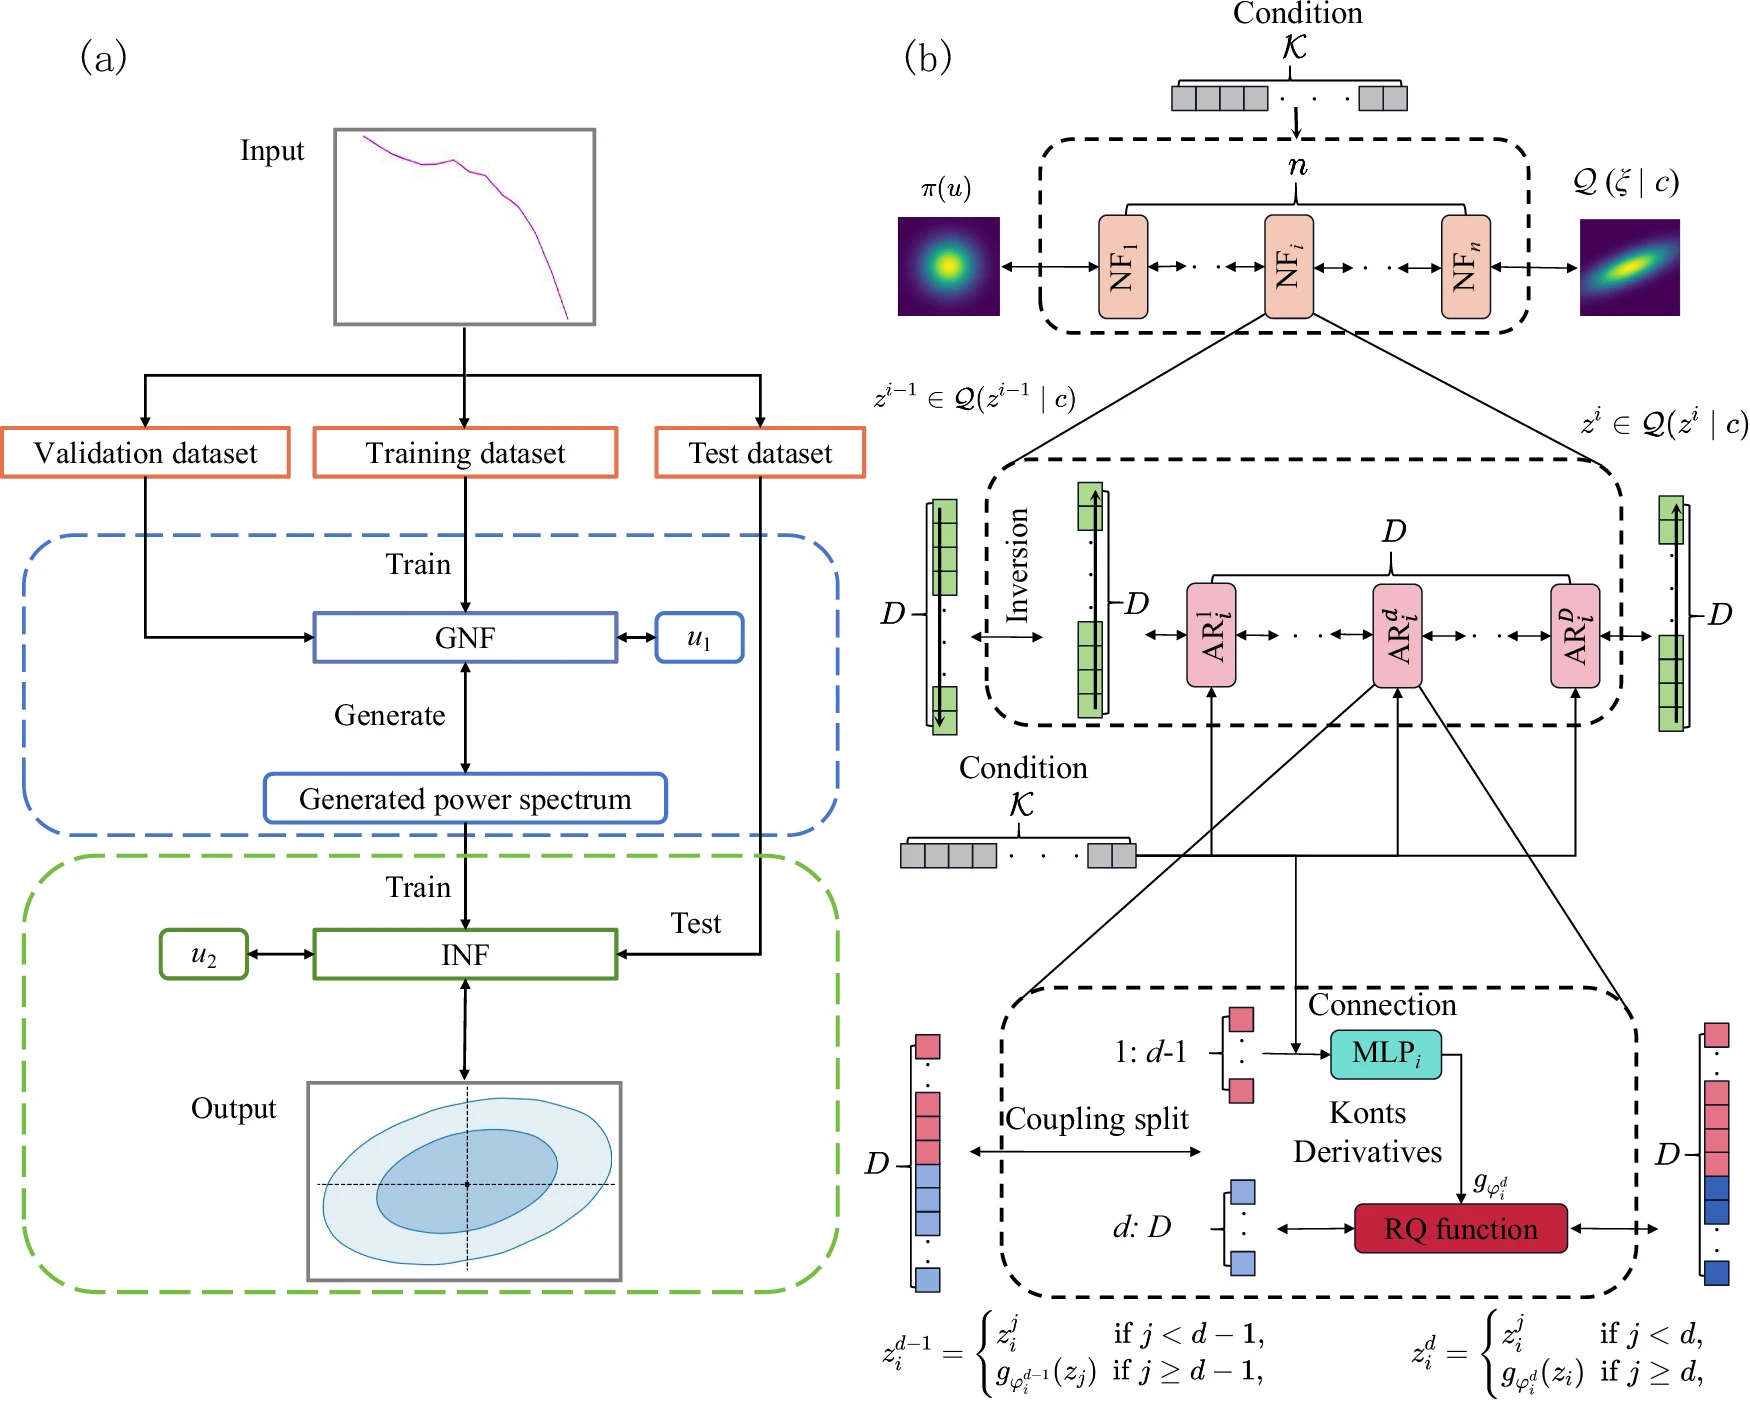
\includegraphics[width=0.96\textwidth]{figures/Sun2025_21cm_fig2.png}
\caption{21cm 森林参数推断中的双流归一化流框架。左图展示从输入功率谱划分训练集、验证集和测试集，并先训练生成归一化流（GNF）扩充模拟样本，再训练推断归一化流（INF）获得参数后验的流程；右图展示条件归一化流及自回归有理二次样条变换模块的结构。该图说明 SBI 方法在“昂贵模拟器+有限训练样本+非高斯后验”问题中的可迁移性。图引自 Sun 等~\cite{sun2025_21cm} 的 Figure 2。}
\label{fig:sbi_transfer_21cm}
\end{figure}

\textbf{CMB功率谱的CVAE异常检测}。跨领域迁移的另一个案例来自宇宙微波背景（CMB）功率谱分析。Sun、Wang 等人~\cite{Sun2025CVAE_CMB}将条件变分自编码器（CVAE）应用于CMB功率谱的宇宙学模型判别与异常检测。CVAE模型能够将CMB功率谱压缩到低维潜在空间，并在其测试设置中实现高保真度重建；对于参数外推情形，其可靠性仍取决于训练覆盖范围和异常判据的校准。这一工作说明，引力波参数估计中发展的CVAE方法论，在结构相近的宇宙学观测问题中也可提供有用工具，并进一步支持“问题结构相似性”是方法迁移成功的重要原因之一。

\textbf{引力波标准汽笛宇宙学综述}。引力波事件作为“标准汽笛”用于宇宙学参数估计，是多信使天文学最重要的科学应用之一。Jin、Wang 等人~\cite{Jin2025GWStandardSirens}系统综述了引力波标准汽笛方法用于哈勃常数等宇宙学参数估计的最新进展，涵盖“亮汽笛”（有电磁对应体）和“暗汽笛”（无电磁对应体）两种方法路线，以及AI方法在提升参数估计精度和处理大样本统计中的关键作用。这一综述为本书第12章关于多信使宇宙学的讨论提供了系统性的文献基础。

\subsection{21cm森林的物理背景与观测挑战}

21cm氢超精细跃迁产生于中性氢原子的电子自旋翻转，静止频率1.42GHz（波长21cm）。高红移（$z=5$--12）的中性氢沿视线方向吸收高红移射电源（如射电类星体）的连续谱辐射，形成“21cm森林”，类似于光学波段的Ly-$\alpha$森林。吸收谱的统计特性（吸收线数密度、等效宽度分布、功率谱）对视线路径上的中性氢密度和气体温度敏感，因此可以约束宇宙再电离历史和暗物质性质。

21cm森林对暗物质性质的约束来自以下物理机制：温暗物质（warm dark matter，WDM）粒子具有非零的自由流长度，会抹平小尺度密度涨落，导致小质量暗物质晕的数量减少。这一效应在21cm森林中表现为：WDM质量越小（自由流长度越大），小尺度吸收特征越少，吸收谱的功率谱在小尺度端越平坦。通过测量21cm森林的功率谱，可以约束WDM粒子质量的下限，目前的约束约为4--5 keV（对应自由流长度约0.1 Mpc）。

21cm森林参数推断面临的主要挑战与引力波参数估计高度相似：模拟代价高昂（单次21cm辐射转移模拟约需1小时，而引力波波形生成约需1毫秒至1秒）；似然函数非高斯（21cm吸收谱的统计分布受非线性结构形成影响，不满足高斯假设）；训练数据稀缺（受计算限制，可用的模拟样本约500条，而引力波参数估计通常使用约 $10^5$--$10^6$ 条训练样本）。

\subsection{SBI迁移的技术实现与结构类比}

Sun等的工作采用双流归一化流架构解决21cm森林参数推断问题。第一个流（生成流）学习从参数空间到观测空间的映射，用于数据增广——从少量真实模拟样本生成大量“虚拟模拟”样本，有效扩充训练集规模。第二个流（推断流）学习从观测空间到参数空间的逆映射，即后验分布 $p(\theta|d)$，用于实际的参数推断。

这一双流架构与引力波参数估计中的SBI方法在结构上高度类比：引力波的观测数据 $d = h(\theta) + n$（信号加噪声），参数 $\theta$ 为源物理参数，模拟器生成 $(\theta, d)$ 对；21cm森林的观测数据为吸收谱，参数为暗物质质量加再电离参数，模拟器生成参数-谱对。两者共享：昂贵模拟、非高斯似然、训练数据稀缺的挑战，以及使用归一化流近似后验分布的技术路线。

在这一迁移过程中，SBI框架的核心思想可以保留，但模拟器（从引力波波形生成器到21cm辐射转移代码）、观测摘要、评估函数（从引力波参数估计精度到21cm功率谱拟合质量）以及校准流程都需要面向新任务重新设计。这种模块化迁移方式，是SBI方法跨领域适用性的一个具体体现。

21cm森林参数推断文章的发表说明，源于引力波数据分析经验的SBI方法已经在独立的物理研究方向上取得同行评议的应用案例，支持了其跨领域应用价值。这提示“引力波AI方法”有机会成为更广泛天文学AI工具箱的一部分，其影响力正在向引力波天文学之外扩展。

SBI方法从引力波到21cm森林的迁移，提示了一个更广泛的方法论原则：在统计推断问题中，“问题结构的相似性”往往比“领域知识的相似性”更有利于方法迁移。引力波参数估计和21cm森林参数推断在物理背景上差异很大——前者涉及强引力场中的致密天体，后者涉及宇宙再电离历史和暗物质性质——但两者共享相近的推断问题结构：给定昂贵的前向模拟器和有限的观测数据，如何高效地推断生成观测数据的物理参数后验分布。这一结构相似性是SBI方法可迁移的重要原因，但并不意味着领域知识可以被忽略；模拟器可信度、观测摘要选择和系统误差建模仍然必须由具体物理问题决定。从这一视角看，SBI方法的跨领域迁移不是简单地“将引力波方法移植到21cm”，而是在两个具体应用场景中实现同一类抽象推断框架。可迁移的是问题求解框架和部分技术组件，而非针对具体问题的完整专用方案。

这一洞察对未来研究有重要启示：引力波数据分析中发展的SBI基础设施（归一化流实现、训练流程、验证框架）可以为其他天文和物理领域提供参考，但通常需要针对领域特定的模拟器、观测数据格式和系统误差重新适配。目前已有初步探索的方向包括：宇宙学大尺度结构的参数推断（用N体模拟替代引力波模拟器）、粒子物理对撞机实验的信号-背景分离（用蒙特卡洛事件生成器替代）、以及地震学中的地壳结构反演（用有限元弹性波模拟替代）。这些方向的进展可能反过来为引力波SBI提供方法论灵感，形成跨领域的方法论共同体。在未来五到十年内，随着跨领域应用积累，“SBI方法学”有望在统计物理、计算天文学和机器学习的交叉处形成更稳定的理论体系和实践规范；引力波数据分析可作为其中较早、较系统的应用场景之一发挥推动作用。

SBI方法跨领域迁移的成功，也给引力波数据分析社区带来了一个重要的学术责任：系统整理和共享方法论工具。当前引力波SBI研究所积累的训练框架、验证工具（PP图生成、覆盖率检验脚本）、和基准数据集，如果能够以开放科学的方式发布，将极大地降低其他领域采用SBI方法的技术门槛，加速跨领域迁移的进程。引力波数据分析社区已经在开放科学方面有良好传统——LIGO-Virgo合作组的引力波事件数据和参数估计结果通过GWOSC（引力波开放科学中心，Gravitational Wave Open Science Center）公开发布，PyCBC、Bilby等分析代码均开源。将这一传统延伸到SBI方法论工具的开放共享，是引力波天文学对整个天文物理AI方法论社区的重要贡献机会。

广义相对论（GR）是迄今最成功的引力理论，但其在强场、高能条件下的完备性仍是开放问题。暗物质、暗能量的存在暗示 GR 可能需要修正，而引力波观测提供了在强场动力学条件下检验 GR 的独特机会。

传统的 beyond-GR 信号搜索面临根本性困难：替代引力理论的数量极多，为每种理论构建专用模板库在计算上不可行。Wang 等人~\cite{wang2025beyondgr} 提出了一种不同的思路：利用在 GR 波形上训练的神经网络的泛化能力，探测偏离 GR 的奇异信号。若网络学习到的是与引力波形态相关的稳健特征，而非训练模板的表面细节，则有可能对部分训练分布之外的信号产生响应。

这一工作的意义超越了具体的方法改进。它展示了 AI 作为弱模型依赖异常筛选工具的潜力：不为每一种替代引力理论预先构建专用模板，而是通过学习已知信号的稳健特征来识别可能偏离训练分布的候选。这一思路与粒子物理中的“模型无关新物理搜索”有相通之处，为 AI 参与基础物理检验提供了新的方法参照。

\subsection{标量-张量引力理论与额外极化模式}

广义相对论预言引力波只有两种极化模式：$+$（plus）极化和 $\times$（cross）极化，对应时空度规的两个独立横向自由度。然而，更广泛的引力理论（如标量-张量理论、$f(R)$引力、Brans-Dicke理论）预言引力波可以有额外的极化模式：标量呼吸模（breathing mode）、标量纵向模（longitudinal mode）、以及矢量模（vector modes）。

在Brans-Dicke理论（最简单的标量-张量理论）中，引力波除了 $h_+$ 和 $h_\times$ 两个张量极化之外，还存在额外的“呼吸模”标量极化。标量极化的振幅与耦合常数 $\omega_{BD}$（Brans-Dicke参数）相关，LIGO对 $\omega_{BD}$ 的约束已达到 $\omega_{BD} > 10^5$，但仍有理论动机探索 $\omega_{BD} \sim 10^3$ 的区间。额外极化的信号特征：频率与张量极化相同（同源辐射），但振幅比 $\epsilon \sim 1/\omega_{BD} \ll 1$，通常远小于张量信号，使得传统模板搜索（仅针对张量极化设计）会系统性地遗漏这类信号。

\subsection{Lorentz破缺与引力子质量的频散效应}

广义相对论预言引力子质量为零，引力波以光速传播，不同频率的引力波以相同速度到达探测器。然而，某些修正引力理论（如双度规引力、Lorentz破缺理论）预言引力子具有非零质量 $m_g$，导致色散关系 $E^2 = p^2c^2 + m_g^2c^4$ 偏离GR的 $E = pc$。

有质量引力子会导致不同频率的引力波以不同速度传播，使得啁啾信号在传播过程中发生频散——低频成分先到达，高频成分后到达，波形的时频关系偏离GR预言。对于传播距离 $D$ 的引力波，频散导致的到达时间差约为：
\begin{equation}
\Delta t \approx \frac{D}{2c} \left(\frac{m_g c^2}{h f}\right)^2,
\end{equation}
其中 $f$ 为引力波频率，$h$ 为普朗克常数。LIGO对引力子质量的约束 $m_g < 1.27 \times 10^{-23}$ eV/$c^2$ 来自对GW150914等事件的相位演化分析。AI检测器通过学习GR波形的典型时频关系，对频散效应引起的偏离天然敏感——任何偏离GR时频关系的信号都会被网络标记为“异常”，无需预先知道偏差的具体形式。

\subsection{Wang等beyond-GR检测的具体结果与方法论意义}

Wang等的beyond-GR检测工作采用了一种“异常检测”（anomaly detection）的思路：在GR双黑洞波形上训练一个自编码器（autoencoder），使其学习GR信号的紧凑表示；对于偏离GR的信号，自编码器的重建误差会显著增大，从而实现检测。

训练集由 $10^5$ 条GR双黑洞波形（注入模拟噪声）组成；测试集包含GR信号和3种beyond-GR信号：额外极化（呼吸模振幅 $\epsilon = 0.01$--$0.1$）、频散效应（引力子质量 $m_g c^2 = 10^{-23}$--$10^{-22}$ eV）、后牛顿偏差（PN系数偏差 $\delta\hat{\phi}_4 = 0.05$--$0.2$）。

在接收者操作特征曲线（ROC）的AUC指标上，对额外极化（$\epsilon=0.1$），检测率约95\%（误报率1\%）；对频散效应（质量 $m_g c^2 = 10^{-22}$ eV），检测率约85\%；对PN偏差（$\delta\hat{\phi}_4 = 0.1$），检测率约90\%。这些结果表明，在该模拟设置中，AI检测器可作为传统模板搜索的补充，用于筛选部分传统模板库难以覆盖的候选信号空间。

这一工作的方法论意义在于：它将引力波数据分析从“验证已知理论”扩展到“探索未知偏差”，为构建较少依赖具体替代理论模板的引力检验工具提供了思路。随着探测器灵敏度的提升和观测事件数量的增加，这类模型无关或弱模型依赖搜索的统计功效有望增强，并可能帮助发现值得进一步精细分析的GR偏差候选或未预期信号。

AI作为弱模型依赖异常筛选工具的价值，在未来的引力波科学中可能随探测灵敏度提升而增长。当探测器能够探测到更远距离（更高红移）的引力波事件时，引力波在传播过程中会对某些偏离GR的效应更加敏感：引力子质量引起的频散效应可随传播距离积累；暗能量或暗物质相关的有效引力修正可能在宇宙学尺度上留下迹象；超出标准模型的新物理（如额外维度）也可能导致传播速度或振幅演化的修正。AI方法若能学习到近距离GR引力波的稳健特征，便可能对某些远距离传播效应引起的异常形态产生响应，从而在缺乏具体理论模板时筛选出值得精细分析的候选事件。这种“AI预筛选+传统精细分析”的两步策略，是未来海量引力波数据中寻找新物理候选的一条可行路径。从实际操作层面看，这一策略的实施需要建立配套的统计框架：AI预筛选输出的“异常候选”需要被赋予统计显著性（如误报率），而后续精细分析的优先级应根据统计显著性和科学价值综合确定。随着AI方法的成熟和验证框架的完善，这一两步策略有望成为未来空间引力波天文台beyond-GR搜索的重要组成部分。

beyond-GR引力波搜索是引力波天文学与基础物理研究的深度交叉点。广义相对论在小尺度（量子引力）和大尺度（暗物质暗能量）两端都面临理论挑战，而引力波探测恰好在两个尺度上都具有灵敏度：双黑洞并合的波形携带了关于紧凑天体附近强引力场（量子引力可能生效的区域）的信息，而引力波在宇宙学距离上的传播则对大尺度引力修正（DE、DM与引力波的耦合）敏感。传统的beyond-GR搜索聚焦于特定理论的具体预言，而人工智能作为弱模型依赖异常筛选工具，可以帮助扩展“偏离GR”候选信号空间，使引力波天文台成为基础物理检验的重要平台之一。随着空间引力波探测器（太极/LISA）的建设，在宇宙学距离（红移$z>5$）上系统性地寻找GR偏差将成为重要的科学目标，而人工智能方法可在候选筛选、异常排序和后续精细分析触发中发挥重要作用。

综合本书各章的工作，可以勾勒出智能化引力波天文学的未来形态。

\textbf{持续智能监测}。未来的引力波天文台将不再依赖人工触发和逐事件分析，而是由 AI 系统持续监测数据流，自动识别信号、估计参数、触发多信使预警。这一系统需要将信号识别（第5章）、参数估计（第6章）、去噪（第7章）、算法自动优化（第8章）有机整合，形成一个自适应的智能管道。

\textbf{自动算法进化}。随着观测数据的积累和噪声特性的变化，数据分析算法需要持续更新。Evo-MCTS 等框架提供了一种机制：以新的观测数据为评估基准，搜索适应当前噪声条件的高性能候选算法，减少完全依赖人工重新设计的负担。

\textbf{跨领域知识融合}。引力波天文学与电磁天文学、中微子天文学、宇宙学的深度融合，将产生新的多信使推断问题。SBI 方法的跨领域迁移能力，使其成为这一融合的天然纽带：同一推断框架可以处理来自不同观测窗口的数据，提取互补的物理信息。

\textbf{人机协作的新模式}。AI 承担算法发现、信号识别、参数估计等计算密集型任务，人类专家专注于科学问题的定义、结果的物理解释、以及新发现的跟进研究。这一分工不是人类被替代，而是人类认知能力的延伸——AI 扩展了人类能够探索的算法空间和信号空间，使科学家能够将精力集中在真正需要物理直觉和创造力的问题上。

\subsection{技术路线图（2025--2035）}

从当前的方法论探索期到未来的工程化成熟期，智能化引力波天文学的技术发展可以划分为三个阶段。

近期（2025--2027年）的重点是完善地面探测器的AI分析管道，建立标准化的SBI推断框架，开展首批太极高保真仿真验证。具体目标包括：在LIGO O4/O5数据或真实噪声注入数据上系统验证SBI方法的统计一致性；建立太极高保真仿真平台（包含TDI实现、时变响应函数、非稳态噪声模型）；完成Evo-MCTS框架在引力波参数估计和去噪任务上的迁移验证。

中期（2027--2030年）的重点是太极/LISA在轨测试数据的AI分析，发展第一代空间引力波在线分析系统，Evo-MCTS框架的系统化和自动化。具体目标包括：实现含100个可分辨银河系双星的中等规模全局拟合（参数维度约 $10^3$）；建立空间引力波数据分析的标准化验证基准（类似地面探测器的MLGWSC-1）；完成三任务（太极+LISA+天琴）联合分析框架的原型验证。

长期（2030--2035年）的重点是面向太极/LISA正式科学运行准备全局拟合管道、多信使联合分析和系统化AI推断。具体目标包括：实现接近任务需求规模的全局拟合原型（可分辨源数约 $10^4$）；建立与SKA等多波段天文台的联合推断平台；完成智能化空间引力波数据处理系统的集成验证，支持从数据采集到候选事件筛选和初步科学产品生成的高度自动化流程。这一三阶段路线图不仅是技术发展的时间表，更是方法论成熟度的评估框架：近期目标对应“单模块验证”阶段，中期目标对应“系统集成原型”阶段，长期目标对应“生产就绪的完整系统”阶段。每个阶段的完成不仅推动了技术进步，也积累了对方法论体系的更深入理解，为下一阶段奠定基础。在这个意义上，本书介绍的方法论创新，都服务于这一更宏大的目标：建造一套能够持续、可靠地探索引力波宇宙的智能化数据分析基础设施。

未来智能化引力波天文台的日常运行将遵循一套人机协作的标准工作流程，在不同时间尺度上分配AI和人类专家的工作。

在秒至分钟的低延迟时间尺度上，AI系统有望承担若干自动化环节：引力波候选体的触发和分类（基于实时信号识别网络）；初步参数估计和天空定位（基于SBI方法或低延迟贝叶斯近似）；多信使预警草案的生成和分发前检查。对于短暂电磁对应体，减少人工和计算延迟十分关键；但预警发布仍需根据数据质量、误报控制和合作组政策设置相应的自动或人工审核机制。

在分钟至小时的时间尺度上，AI辅助人类完成：精确参数估计和不确定度量化（混合AI+贝叶斯，约1--3小时）；信号真实性的交叉验证（多探测器一致性检验、与已知噪声源的对比）；异常事件的专项分析（beyond-GR信号候选、未预期信号形态）。这一层次的人机协作确保了科学结论的可靠性，避免了纯自动化系统可能产生的系统性误差。

在天至周的时间尺度上，人类专家主导：物理解释和科学结论（引力波源的天体物理意义、对基础物理的约束）；算法优化和方法论更新（Evo-MCTS周期性自动优化，人类专家季度审查）；科学论文的撰写和同行评审。这一层次的人类主导确保了科学发现的深度和可信度，是AI无法替代的核心价值所在。

\subsection{下一代技术的潜在影响}

除本书系统介绍的方法之外，若干新兴 AI 技术在引力波数据分析中具有重要的潜在价值，值得在此展望。

\textbf{扩散模型（Diffusion Models）}。近年来在图像生成领域取得突破性进展的扩散模型，其核心思想是学习从噪声分布到目标分布的去噪路径，天然适合引力波去噪任务。与 WaveFormer 等判别式去噪方法不同，扩散模型是生成式的：它能够为同一含噪输入生成多个去噪样本，从而提供去噪结果的不确定度估计。这一特性对于评估去噪后参数估计的可靠性具有重要意义。扩散模型用于 SBI 也正在成为活跃的研究方向，其在 EMRI 等多模态后验分布的建模上可能优于标准归一化流。

\textbf{基础模型（Foundation Models）}。大语言模型在代码生成和候选算法搜索方面的能力，已通过 Evo-MCTS 框架在引力波算法发现中得到初步验证。更进一步，针对物理科学数据训练的“物理基础模型”（physics foundation model）——在大量物理模拟数据上预训练的通用模型——有望提供一种更统一的数据分析范式：从原始或低级预处理后的探测器数据中学习通用表示，再服务于检测、参数估计、去噪和异常识别等下游任务。其科学使用仍需要严格的物理约束、校准验证和可解释性评估。

\textbf{多模态天文学中的 AI 协同}。随着电磁天文台（SKA、ELT、CSST）和中微子探测器（IceCube）灵敏度的持续提升，多信使天文学将从“偶发的联合观测”演变为“系统性的跨波段推断”~\cite{Abbott2017GW170817}。引力波数据分析中发展的 SBI 框架，与电磁和中微子观测的联合推断，是这一方向的自然延伸：同一贝叶斯框架可以同时处理来自不同探测器的数据，提取关于引力波源的互补物理信息——例如，同时利用引力波信号确定双中子星并合的质量参数，利用千新星光变曲线约束核物质状态方程，利用短伽马射线暴喷流结构推断黑洞自旋。

\textbf{量子计算的远期展望}。量子计算在某些特定类型的组合优化、采样和线性代数问题上具有理论加速可能。对于引力波数据分析中的某些高维积分或模板放置问题，量子蒙特卡洛、量子退火或量子近似优化算法可以作为远期探索方向。尽管这一方向目前仍处于基础研究阶段，距离实际应用尚有较大距离，且尚无引力波数据分析中的量子优势实验证据，但量子计算与 AI 方法的结合（量子机器学习）仍是远期技术路线图中值得关注的方向。

引力波天文学的未来，是人类智慧与人工智能深度协作的未来。本书所呈现的方法论体系，正是这一协作的早期实践与系统总结。

在科学目标层面，未来十年内最令人期待的进展包括以下几个方向。第一，引力波背景的多频段观测：脉冲星计时阵列（PTA）在纳赫兹频段已发现随机引力波背景的候选信号，太极/LISA在毫赫兹频段可能探测到宇宙相变或弦网络背景，两者的联合约束将为早期宇宙物理提供新的观测窗口。第二，极端质量比旋近的第一批系统性探测：EMRI是空间引力波探测器的“旗舰”科学目标，每个EMRI事件携带的强引力场信息相当于在黑洞附近进行数十万圈的精密轨道力学测量，AI方法（特别是CNF参数估计）是使这一科学目标从“理论上可能”变为“实际可分析”的关键使能技术。第三，多信使宇宙学：利用引力波事件作为“标准汽笛”对宇宙学距离进行测量，既包括有电磁对应体的“亮汽笛”，也包括依赖星系目录和统计关联的“暗汽笛”。当事件数量和星系红移信息足够丰富时，哈勃常数测量精度有望逐步接近百分之几乃至百分之一量级，为检验哈勃张力提供独立信息。

从方法论演进的角度看，AI在引力波天文学中的应用正在从“方法移植”（将通用AI方法移植到引力波场景）向“方法创生”（由引力波特定问题催生新的AI方法论范式）演进。MF-CNN的感知层设计、SBI与贝叶斯的精确协同、Evo-MCTS的可解释算法自动发现，都是引力波物理的独特挑战催生的方法论创新，这些创新反过来又为更广泛的科学AI方法论贡献了新的视角和工具。这种从“领域应用”到“方法创生”的转变，标志着引力波数据分析已经从AI技术的“消费者”成长为AI方法论的“生产者”。

\begin{table}[htbp]
\centering
\caption{引力波天文学AI方法论里程碑总结}
\label{tab:ai_milestones}
\small
\begin{tabular}{llll}
\hline
\textbf{方法} & \textbf{代表工作} & \textbf{关键成果} & \textbf{科学意义} \\
\hline
MF-CNN & Wang等 (2020) & 识别O1/O2多数确认事件 & 物理先验嵌入范式 \\
集成学习 & Ma等 (2022) & 跨轮次低误报泛化 & 鲁棒性验证 \\
SBI归一化流 & Wang等 (2022) & 高维参数估计加速 & 推断范式转变 \\
WaveFormer & Wang等 (2024) & 全局时频特征捕获 & Transformer在GW去噪中的应用 \\
CNF-EMRI & Liang等 (2024) & 17维参数估计探索 & 空间GW分析可行化 \\
混合推断 & Sun等 (2025) & 采样时间压缩至14\% & 精确协同范式 \\
Evo-MCTS & Wang等 (2025) & 超越既有ML基线20.2\% & AI驱动算法发现 \\
\hline
\end{tabular}
\end{table}

\section{下一代探测器与人工智能方法的协同演化}

\begin{figure}[htbp]
\centering
\resizebox{0.98\textwidth}{!}{%
\begin{tikzpicture}[
  font=\small,
  milestone/.style={draw, rounded corners=3pt, text width=25mm, minimum height=10mm,
                    text centered, align=center, fill=blue!8, draw=blue!45,
                    font=\scriptsize, inner sep=2.5pt},
  future/.style={draw, rounded corners=3pt, text width=25mm, minimum height=10mm,
                 text centered, align=center, fill=orange!10, draw=orange!60,
                 dashed, font=\scriptsize, inner sep=2.5pt},
  arr/.style={-Stealth, thick, gray!60},
]
% 时间轴
\draw[-Stealth, very thick, gray!55] (0,0) -- (15.2,0)
  node[right,font=\scriptsize,gray!70]{时间};
\foreach \x/\yr in {0.8/2020, 3.2/2022, 6.4/2024, 9.8/2025, 12.6/2030, 14.4/2035} {
  \draw[gray!45, thin] (\x,-0.12) -- (\x,0.12);
  \node[font=\scriptsize, gray!75] at (\x,-0.35) {\yr};
}

% 里程碑
\node[milestone] (mfcnn) at (0.8,1.35) {MF-CNN\\物理先验嵌入};
\node[milestone] (normflow) at (3.2,-1.35) {归一化流\\SBI参数估计};
\node[milestone] (waveformer) at (5.6,1.35) {WaveFormer\\Transformer去噪};
\node[milestone] (cnfemri) at (7.5,-1.35) {CNF-EMRI\\17维参数估计};
\node[milestone] (evomcts) at (10.0,1.35) {Evo-MCTS\\自动算法发现};

% 未来里程碑
\node[future] (globalfit) at (12.5,-1.35) {全局拟合原型\\$10^4$量级联合推断};
\node[future] (realtime) at (14.2,1.35) {实时智能管道\\低延迟自动化};

% 连接线
\draw[arr] (0.8,0.12) -- (mfcnn.south);
\draw[arr] (3.2,-0.12) -- (normflow.north);
\draw[arr] (5.6,0.12) -- (waveformer.south);
\draw[arr] (7.5,-0.12) -- (cnfemri.north);
\draw[arr] (10.0,0.12) -- (evomcts.south);
\draw[arr, dashed, orange!70] (12.5,-0.12) -- (globalfit.north);
\draw[arr, dashed, orange!70] (14.2,0.12) -- (realtime.south);
\end{tikzpicture}}
\caption{引力波AI方法论里程碑时间线。蓝色实线框为本书讨论的已发表或已完成研究工作，橙色虚线框为面向下一代探测器和空间引力波任务的阶段性研究目标。从MF-CNN到Evo-MCTS，相关工作展示了从“物理先验嵌入”到“自动算法发现”的方法论拓展；未来节点为路线图式概括，并非任务正式时间表。代表性工作参见文献~\cite{wang2020deeplearning,wang2022normflow,wang2024waveformer,liang2024cnfemri,sun2025cvae,wang2025evomcts,wang2024challenges,du2026taiji}。}
\label{fig:ai_timeline}
\end{figure}

下一代地面引力波探测器——爱因斯坦望远镜（ET）~\cite{Punturo2010ET} 和宇宙探索者（CE）~\cite{Evans2021CE}——计划在2030年代推进建设，其灵敏度目标比 Advanced LIGO 提升约一个量级，预期事件率可能达到每年 $10^5$ 量级或更高。这一量级的事件率将使当前的逐事件人工分析模式难以维系，人工智能方法有望从“辅助工具”发展为数据分析基础设施中的核心组成部分。

\textbf{ET/CE 对数据分析的新要求}。ET 采用三角形地下配置，三条臂长10公里的干涉仪，低频截止目标约2--3 Hz，使其能够探测更长的双中子星旋进信号和更高红移的双黑洞。CE 采用L型配置，臂长40公里，在宽频段提供高灵敏度，与ET形成互补。两者联合运行时，双中子星和双黑洞事件数将大幅增加，其中一部分可望具有电磁对应体，多信使天文学将从“偶发事件”演变为“统计样本”。

对数据分析的新要求体现在三个方面：（1）\textbf{实时性}——多信使预警需要在并合前或并合后极短时间内完成参数估计，SBI方法的快速推断提供了一条具有吸引力的技术路线；（2）\textbf{可扩展性}——每年 $10^5$ 量级事件的参数估计需要高度自动化的流水线，人工干预应主要集中于科学价值最高或最异常的事件；（3）\textbf{精度}——更高灵敏度意味着更高信噪比，参数估计精度要求相应提升，SBI方法的精度验证（PP图检验）将成为科学可信度的重要保障。

\textbf{AI方法的协同演进路径}。面向ET/CE时代，AI方法需要在以下方向协同演进：归一化流架构需要扩展到更高维度（包含潮汐形变参数的BNS系统约17维）；训练数据需要覆盖更宽的参数范围（高红移、高质量比、高自旋）；实时推断系统需要与多信使预警基础设施深度集成；可靠性工程需要建立与经典方法等同级别的验证框架。这些演进方向，正是本书各章方法论工作的自然延伸，也是未来引力波AI研究最重要的工程目标。

\begin{table}[htbp]
\centering
\caption{下一代引力波探测器与AI方法需求对比}
\label{tab:next_gen_detectors}
\small
\begin{tabular}{lcccc}
\hline
\textbf{探测器} & \textbf{臂长} & \textbf{低频截止} & \textbf{年事件率} & \textbf{AI关键需求} \\
\hline
Advanced LIGO O4 & 4 km & $\sim$10 Hz & 百量级公开候选 & 辅助加速 \\
爱因斯坦望远镜（ET） & 10 km（地下） & $\sim$2--3 Hz & $\sim 10^5$量级 & 高度自动化 \\
宇宙探索者（CE） & 40 km & $\sim$5 Hz & $\sim 10^5$量级 & 高度自动化 \\
太极/LISA & 百万 km（空间） & 毫赫兹窗口 & 依源类而定 & 全局拟合 \\
\hline
\end{tabular}
\end{table}

\section{量子传感与引力波探测的未来}

引力波探测的灵敏度提升，在经典物理框架内已接近基本极限。地面引力波探测器的噪声预算由量子噪声（散粒噪声和辐射压力噪声）、热噪声和地震噪声共同决定，其中量子噪声在宽频段内占主导地位。突破经典极限、进入量子增强探测的新时代，是下一代引力波探测器的核心技术挑战，也是量子光学、原子物理与引力波天文学深度交叉的前沿领域。

\subsection{量子压缩光的现状与前景}

量子压缩光技术是目前最成熟的量子增强引力波探测方案，已在Advanced LIGO的O3观测运行中实现了工程化应用。在标准量子极限（SQL）框架下，迈克尔逊干涉仪的量子噪声由海森堡不确定性原理约束：
\begin{equation}
\Delta x \cdot \Delta p \geq \frac{\hbar}{2},
\end{equation}
其中$\Delta x$为位置（相位）不确定度，$\Delta p$为动量（振幅）不确定度。标准相干光的量子噪声在相位和振幅两个正交分量上均等分布；压缩光通过非线性光学过程（参量下转换）将量子噪声从相位分量“压缩”到振幅分量，从而在牺牲振幅精度的代价下提升相位（即引力波信号）的测量精度。

Advanced LIGO O3运行期间，注入15 dB的压缩光（对应量子噪声降低约$10^{15/10}\approx32$倍的功率，即约5.6倍的振幅）使探测器在高频段（$>$50 Hz）的灵敏度提升约3倍信噪比~\cite{Tse2019squeezing}。这一成果标志着量子增强引力波探测从实验室演示走向实际科学运行的历史性跨越。然而，15 dB压缩在实践中受到光学损耗（镜面散射、吸收）和相位噪声的严格限制，进一步提升压缩度面临工程上的系统性挑战。

量子反作用规避（Quantum Non-Demolition，QND）技术代表了超越标准量子极限的更深层次方案。在标准迈克尔逊干涉仪中，测量光子对镜面施加辐射压力，产生量子反作用噪声；在高功率运行时，辐射压力噪声与散粒噪声的乘积恰好等于标准量子极限。QND技术通过设计特殊的光学配置，使辐射压力噪声与散粒噪声之间产生量子相关（quantum correlation），从而在原理上突破标准量子极限。变速光（speed meter）配置是QND技术的一种具体实现：通过在干涉仪中引入额外的“速度测量”光路，使探测器对镜面速度（而非位置）敏感，从而规避辐射压力反作用的影响。理论分析表明，理想的QND探测器可以将灵敏度提升至海森堡极限：
\begin{equation}
\Delta x_{\rm Heisenberg} = \frac{\hbar}{2\Delta p} \propto \frac{1}{\sqrt{N_{\rm photon}}},
\end{equation}
其中$N_{\rm photon}$为探测光子数，对应灵敏度随光功率的平方根提升，而非标准量子极限下的线性关系。爱因斯坦望远镜（ET）和宇宙探索者（CE）的设计方案均将QND技术列为核心技术路线，预期在2030年代实现工程化验证。

\subsection{原子干涉引力波探测器}

原子干涉仪利用超冷原子的物质波干涉效应测量引力波引起的时空应变，代表了不同于激光干涉仪的技术路线。在原子干涉仪中，激光脉冲将原子波包分裂、偏转和重合，形成类似于光学迈克尔逊干涉仪的干涉结构；引力波引起的时空应变改变了两条原子路径的相对相位，从而在干涉条纹中留下可测量的信号。原子干涉仪的潜在优势在于：原子的内部量子态（超精细能级）可提供稳定的相位参考，并在特定设计下改善低频加速度噪声（地震噪声、重力梯度噪声）对测量的影响。

当前国际上主要的原子干涉引力波探测器项目包括：英国的AION（Atom Interferometer Observatory and Network）~\cite{Badurina2020AION}，计划建设10米、100米和1公里三个尺度的原子干涉仪，逐步验证从实验室到引力波探测的技术路线；美国的MAGIS（Mid-band Atomic Gravitational wave Interferometric Sensor）~\cite{Graham2017MAGIS}，利用斯坦福大学的100米垂直塔开展原型验证，目标是在0.1--10 Hz的中频段实现引力波探测；中国的ZAIGA（Zhaoshan Long-baseline Atom Interferometer Gravitation Antenna）~\cite{Zhan2020ZAIGA}，依托武汉赵山地下实验室建设，利用地下环境的低地震噪声优势，计划实现基线长度达数百米的原子干涉仪网络。

原子干涉引力波探测器的独特科学价值在于其对中频段（0.1--10 Hz）的灵敏度。这一频段恰好处于地面激光干涉仪（灵敏频段$>$10 Hz）和主要面向毫赫兹频段的空间激光干涉仪之间，是当前引力波探测网络的重要盲区。中频段的主要科学目标包括：中等质量黑洞（IMBH，$10^2$--$10^5\,M_\odot$）的并合信号——这类天体的存在是连接恒星质量黑洞（$\sim$10$M_\odot$）和超大质量黑洞（$>10^6\,M_\odot$）的关键环节，但迄今尚无确凿的引力波探测证据；双中子星并合的早期旋近阶段——在地面探测器灵敏频段之前数小时至数天，原子干涉仪可以提前预警，为多信使观测提供充裕的准备时间；以及宇宙学引力波背景的中频段成分，对早期宇宙相变和宇宙弦网络的约束能力远超现有探测器。

\subsection{量子网络与引力波天文学}

量子网络技术与引力波天文学的交叉，开辟了超越单台探测器灵敏度极限的新可能性。量子纠缠辅助的探测器网络是一个远期设想：通过在地理上分离的探测器之间分发量子关联资源，理论上可改善联合测量的量子噪声表现。由于长距离纠缠分发、光学损耗、相位稳定和探测器耦合都极具挑战，这一方向目前主要停留在理论和概念验证阶段。

量子通信技术在引力波预警系统中的应用，目前更接近信息安全层面的远期设想。当前引力波预警系统依赖经典通信网络传输候选事件和天空定位信息，其主要瓶颈通常来自数据处理、候选审核和望远镜调度，而非加密方式本身。量子密钥分发（QKD）可为高安全需求的科学通信提供一种可能方案，但它不是提升多信使预警时效性的核心技术路径。

量子计算加速引力波数据分析，是量子技术与引力波天文学交叉中具有长期潜力、但也高度不确定的方向。量子机器学习算法在特定输入模型和数据访问假设下可能提供复杂度优势，量子蒙特卡洛方法也可能加速某些高维积分估计。然而，这些理论优势往往依赖强假设（如高效量子数据加载、低噪声深电路或特定问题结构），目前尚不能直接转化为引力波参数估计或搜索流水线中的实际加速。

\subsection{AI与量子技术的协同}

量子机器学习用于引力波参数估计的理论可行性，是近年来量子计算与引力波天文学交叉研究的核心问题。量子神经网络（QNN）通过参数化量子电路（PQC）实现类似经典神经网络的函数逼近能力，其表达能力在理论上由量子电路的纠缠结构决定。对于引力波参数估计问题，QNN的潜在优势在于：量子态的希尔伯特空间维度随量子比特数指数增长，使得QNN在原理上可以用较少的参数表达经典神经网络需要大量参数才能表达的复杂函数；量子纠缠可以自然地编码引力波参数之间的相关性（如质量比与自旋之间的简并），从而提升参数估计的效率。

然而，量子优势的实际实现面临近期量子计算机的严峻限制。当前NISQ设备虽然已具备数百到上千量级物理量子比特的实验平台，但量子退相干、门错误率和读出误差限制了可执行电路深度；容错逻辑量子比特的规模仍远不足以处理引力波参数估计这类复杂科学计算问题。更根本的挑战在于：许多量子机器学习的理论加速优势依赖于高效量子数据加载或QRAM，而这些条件在实际硬件上仍是开放工程难题。

从更现实的近期视角来看，量子-经典混合算法（variational quantum algorithms，VQA）代表了在NISQ时代最有可能实现实际应用的量子计算路线。VQA将量子电路用于计算经典计算机难以高效处理的特定子任务（如量子态制备、量子核函数计算），而将优化和后处理留给经典计算机，形成量子-经典协同的计算架构。在引力波数据分析中，VQA的潜在应用包括：利用量子核方法加速引力波信号的特征提取、利用量子采样加速贝叶斯后验的低维投影计算，以及利用量子优化算法改进引力波模板库的覆盖策略。

AI与量子技术的协同，在更深层次上体现为两种技术路线的互补性：AI方法（特别是深度学习和SBI）擅长处理高维、非线性的数据分析问题，但受限于经典计算资源；量子计算在特定问题上具有理论加速潜力，但受限于当前量子硬件的噪声和规模。两者的协同可以从识别适合量子加速的低维子任务开始，例如小规模组合优化、低维积分或核函数估计。这一融合的实现，需要引力波物理学家、量子计算研究者和AI研究者的深度跨学科合作，也需要量子硬件技术的持续进步。就当前技术状态而言，它更应被视为长期探索方向，而非太极/LISA早期数据处理的近期方案。

\section{引力波天文学与多信使科学的深度融合}

多信使天文学（multi-messenger astronomy）是引力波天文学最重要的科学应用场景之一，也是AI方法发挥关键作用的核心领域。GW170817双中子星并合事件的成功多信使观测，已经展示了引力波与电磁波联合分析的巨大科学价值；而未来随着探测器灵敏度的提升和AI方法的成熟，多信使天文学将从“偶发事件”演变为“系统性科学”。

\textbf{多信使预警的时效性要求}。双中子星并合事件在并合前数分钟至数小时内，旋进阶段的引力波信号已经进入LIGO/Virgo的灵敏频段。对于典型的BNS系统（总质量约$2.8\,M_\odot$），信号在并合前约15分钟进入10 Hz频段，在并合前约1分钟进入100 Hz频段。如果能在并合前数分钟内完成参数估计并发出预警，电磁望远镜可以提前指向目标天区，捕捉并合瞬间的伽马射线暴（GRB）和千新星（kilonova）的早期辐射——这些早期辐射携带了关于中子星物质状态方程和重元素核合成的关键信息，是事后观测无法获取的。

SBI方法的快速推断速度，使并合前实时参数估计成为有吸引力的技术目标。一个可设想的流程是：在线匹配滤波或CNN检测器识别BNS候选体，SBI归一化流给出快速近似参数后验，BAYESTAR等低延迟天空定位工具给出初步定位，然后向全球电磁望远镜网络发送预警。实际总延迟取决于信号进入频段的时间、触发阈值、数据质量检查、人工或自动审核策略以及望远镜调度系统，因此不宜用单一固定时间概括；但AI快速推断有望压缩其中的参数估计环节。

\textbf{引力波标准汽笛与哈勃常数测量}。引力波事件提供了一种独立于传统距离阶梯的宇宙学距离测量方法——“引力波标准汽笛”（gravitational wave standard siren）。双中子星并合事件的引力波波形直接编码了光度距离信息（通过波形振幅），无需依赖传统距离阶梯校准。结合电磁对应体确定的宿主星系红移，可以独立测量哈勃常数$H_0$。GW170817给出$H_0$的十余个百分点精度约束；随着BNS事件数量、星系红移目录和暗汽笛统计方法的发展，标准汽笛有望逐步提高$H_0$测量精度，并为检验CMB测量与传统距离阶梯测量之间的“哈勃张力”提供独立证据；可达到的具体精度仍取决于事件样本、宿主星系关联、选择效应和系统误差控制。

AI方法在标准汽笛分析中的关键作用体现在两个方面：其一，SBI方法对BNS事件的快速参数估计（特别是距离和倾角的联合后验），有助于积累大样本统计；其二，机器学习方法对宿主星系候选筛选、星系目录匹配和红移信息整合具有潜在价值，可在没有明确电磁对应体的情况下通过统计方法（“暗汽笛”方法）利用更多引力波事件约束$H_0$。

\textbf{中子星状态方程的多信使约束}。双中子星并合事件对中子星物质状态方程（EOS）的约束，是多信使天文学最重要的核物理科学目标之一。引力波波形在并合前最后几个轨道周期内对潮汐形变率$\Lambda$敏感，$\Lambda$反映了中子星的内部结构（半径和可压缩性）。GW170817对$\Lambda$的测量已将典型中子星半径约束到十余公里量级，并排除了一部分极端状态方程。未来ET/CE时代，多事件联合分析有望显著改善半径和EOS参数约束，但具体精度取决于事件数、信噪比分布、波形系统误差和电磁对应体信息。

AI方法在EOS约束中的作用包括：SBI方法对包含潮汐形变参数的BNS波形（约17维参数空间）的快速参数估计；机器学习方法对千新星光变曲线的自动分析（约束重元素产率和喷射物质量）；以及贝叶斯层级分析框架对大量BNS事件的联合EOS约束。这些方法的协同，将使多信使BNS分析从“单事件精细研究”升级为“大样本统计科学”，是引力波天文学与核物理学深度融合的技术基础。

\section{本章小结}

本章从四个维度展望了智能化引力波天文学的发展趋势：LLM驱动的自动算法发现、SBI方法的跨领域迁移、弱模型依赖信号探测，以及智能化天文学的未来形态。人工智能在引力波天文学中的角色演变不是线性改进，而是结构性扩展——从“计算工具”到“方法协作者”，从“单领域专用”到“跨领域迁移”，从“事后分析”到“低延迟预警”。这三重转变，共同定义了智能化引力波天文学的主要特征，也指向了未来引力波AI研究的重要发展方向。

引力波天文学在AI方法论发展中的独特贡献，部分来自其数据特性的独特组合：信号形态有精确的物理理论支撑（广义相对论+数值相对论），噪声特性有可量化的统计模型，评估标准客观明确且国际公认（MLGWSC-1等挑战赛），物理可解释性要求极为严格（因为科学结论需要同行信任）。这一独特组合使引力波数据分析成为AI方法论探索的理想试验场——既有足够的复杂度来挑战AI方法的能力边界，又有足够的物理约束来验证AI方法的可信度。未来，随着引力波AI方法论的成熟，这一试验场将向更广泛的天文学和物理学领域辐射，推动科学AI方法论从引力波天文学走向更宏大的科学舞台。

引力波天文学与人工智能的深度融合，在更广泛的意义上代表了当代科学探索的一种新范式：面对数据规模和复杂度持续超越人类直接分析能力的科学问题，人工智能不是替代科学家，而是以“认知放大器”的形式扩展科学家的探索能力。引力波数据分析中的AI应用已经展示了这种放大效应的多个维度：计算速度的放大（SBI将若干参数估计任务压缩多个量级）、探索广度的放大（Evo-MCTS在人类难以穷举的算法空间中发现新解）、以及感知深度的放大（可解释性分析揭示网络学到的物理相关特征）。这三个维度的放大，共同构成了智能化引力波天文学的重要方法论基础。

回顾本书记录的方法论演进，从2020年的MF-CNN到2025年前后的Evo-MCTS，引力波AI方法论经历了从“单点性能优化”到“方法论体系建设”的明显推进。这一推进不是由单个结果驱动的，而是多个方向研究的协同积累：可解释性研究建立了物理-AI一致性的验证框架，SBI方法缓解了计算瓶颈，Evo-MCTS展示了自动算法发现的新可能。未来的引力波AI研究，需要在这一基础上继续深化：更精密的可解释性分析（从“定性验证”到“定量约束”）、更可靠的SBI精度保证（从“经验验证”到“理论保证”）、更广泛的自动算法发现应用（从“单任务原型”到“多任务系统”）。这三个方向的协同深化，将支撑太极/LISA时代的海量科学数据处理。

引力波AI方法论的成熟，将从三个层面改变引力波天文学的科学实践模式。在个体研究者层面，AI工具的普及有望降低引力波数据分析的技术门槛，使更广泛的科学社区能够参与这一领域；在合作组层面，AI自动化流水线将压缩从数据采集到初步科学结论的时间周期，加快候选事件筛查和后续观测触发；在学科层面，AI方法的跨领域迁移能力（引力波→21cm森林→更多宇宙学观测）将推动引力波数据分析方法论成为更广泛的天文学AI基础设施的一部分。

第11章的核心论点是：人工智能在引力波天文学中的角色演变不是线性改进，而是结构性扩展。从“计算工具”到“方法协作者”的转变，体现在Evo-MCTS等方法能够搜索候选算法、beyond-GR探测能够作为弱模型依赖检验的辅助工具、SBI方法能够迁移到21cm森林等宇宙学观测问题。LLM驱动的自动算法发现揭示了两条原则：可迁移的是搜索机制而非固定管道，领域知识集成是决定成败的关键因素。智能化引力波天文学的未来形态包括持续智能监测、自动算法优化、跨领域知识融合和人机协作新模式；其核心是扩展人类能够探索的算法空间和信号空间，而非替代人类的物理直觉和创造力。

\chapter{结语：面向可信智能引力波天文学}

\section{本书主要贡献总结}

本书以“人工智能与统计推断的交叉融合”为主线，系统梳理了引力波天文学数据分析方法论的前沿进展。从第一部的理论基础出发，经由第二部对经典方法局限性的深入分析，到第三、四部对 AI 新方法及其与物理融合的系统介绍，最终以第五部对未来挑战与发展趋势的展望收尾——全书构成一个逻辑完整、层次递进的方法论体系。

本书写作的学术背景，是引力波天文学从发现阶段走向大样本和空间探测阶段的关键时期：从2015年GW150914的首次直接探测，到即将到来的太极/LISA空间引力波探测器时代，数据分析面临的计算挑战从“困难但可解决”演变为“直接传统流程难以承担”。正是这种现实需求，驱动了本书所介绍的每一个方法论创新——每一项创新都不是为了创新而创新，而是为了解决引力波天文学前进道路上的具体障碍。这种“问题驱动的方法论创新”精神，贯穿了本书的始终，也是评价这些方法论价值的正确标准。

引力波天文学的成功，既是探测器技术的胜利（将应变灵敏度提升至$10^{-23}$量级），也是数据分析方法的胜利（从海量噪声数据中提取微弱的时空信号）。本书所记录的人工智能方法论创新，是这一数据分析方法演进中的重要组成部分。它们的价值不在于制造技术噱头，而在于把新的计算工具放回引力波天文学的严格物理和统计约束之中，检验其是否真正能够服务于可靠的科学发现。

在方法论层面，本书的核心贡献可以归纳为三条主线。

\textbf{第一条主线：从黑箱到可解释}。早期深度学习方法在引力波数据分析中以高效见长，但决策逻辑对物理学家不透明。本书系统介绍了可解释性的多种实现路径：感知层设计将物理先验以归纳偏置的形式嵌入网络结构~\cite{wang2020deeplearning}（第5章）；随机森林特征分析揭示了 CNN 关注的物理特征~\cite{tian2025cnn}（第5、9章）；Evo-MCTS 框架通过树结构进化搜索，直接发现由可检视模块组成的算法~\cite{wang2025evomcts}（第8章）。这一从“黑箱”到“可解释”的演进，是引力波 AI 方法走向实际科学应用的必经之路。

\textbf{第二条主线：从近似替代到精确协同}。SBI 方法（第6章）和混合推断策略（第6、9章）展示了 AI 与经典贝叶斯方法的一种有代表性的合作模式：神经网络不是替代贝叶斯推断，而是作为快速先验约束工具，在特定实验设置中将精确贝叶斯采样的计算代价压缩至 14\%~\cite{sun2025cvae}。这一“精确协同”范式，相比单纯的“近似替代”更容易满足科学可信度和可校准性的要求。

\textbf{第三条主线：从单一方法到自动发现}。Evo-MCTS（第8章）代表了一种新的方法搜索范式：在由人类专家定义的搜索空间、评估指标和物理约束下，由 LLM 引导的进化搜索提出候选算法~\cite{wang2025evomcts}。在 MLGWSC-1 基准~\cite{schafer2023mlgwsc1}上 20.2\% 的性能提升，说明“AI 辅助算法发现”可以在受控基准中形成可检验的研究路径。

本书系统介绍的方法论体系在科学可信度方面也进行了建设，这是AI方法在严肃科学中应用的重要前提，却往往在方法论论述中被忽视。可信度建设体现在三个层面：统计验证层面，PP图、覆盖率检验、Gelman-Rubin统计量等工具被用于检验AI方法的统计一致性；物理验证层面，遮罩实验、随机森林特征分析、beyond-GR泛化测试等工具被用于考察AI方法的物理一致性；工程验证层面，MLGWSC-1等标准化挑战赛提供了与独立基线的客观比较，增强了性能声明的可重复性。这三个层面的系统验证，构成了引力波AI方法科学可信度的闭环，也是本书对引力波AI方法论的重要贡献之一。科学可信度的建设不应被视为方法开发完成后的附加环节，而应贯穿整个方法论体系的设计之中：从最初的网络架构选择（物理先验的嵌入方式决定了可解释性的深度），到训练策略的制定（训练集的代表性决定了统计一致性的范围），到验证实验的设计（挑战赛的规范性决定了性能声明的可信度）。这种“可信度优先”的方法论设计理念，是引力波数据分析对科学AI方法论的重要贡献之一。

\subsection{MF-CNN的方法论意义}

MF-CNN的核心贡献不仅是“更快的引力波检测器”，而是提供了一个示范性的方法论框架——如何将物理先验以“软约束”（归纳偏置）而非“硬约束”的形式嵌入神经网络~\cite{wang2020deeplearning}。传统的物理约束通常以硬约束的形式出现：要求网络输出满足特定的物理方程，或者在损失函数中加入物理约束项。这种硬约束方式虽然保证了物理一致性，但限制了网络的表达能力，可能导致在复杂噪声条件下的性能下降。

MF-CNN的感知层设计采用了不同的思路：将匹配滤波的三步操作（白化、模板卷积、归一化）实现为可学习的卷积单元，使网络在初始化时具有匹配滤波的行为，但在训练过程中可以根据数据自适应调整。这种“软约束”方式既保留了物理先验的指导作用，又允许网络学习超越匹配滤波的特征表示，在真实噪声条件下表现出更强的鲁棒性。

这一框架的可迁移性在于：许多具有已知物理结构的信号处理问题都可以借鉴类似的“感知层”设计思路。在引力波去噪（WaveFormer）、EMRI检测（两层CNN）、以及空间引力波全源检测（多阶段自注意力网络）中，都可以看到类似的物理先验嵌入策略。对可解释性的贡献同样重要：通过设计物理上有意义的网络结构，MF-CNN的决策逻辑对物理学家更透明、更容易验证，为AI方法在科学应用中的可信度建设提供了基础。

\subsection{SBI方法体系的贡献层次}

SBI方法体系的贡献可以从技术、方法论、科学和跨领域四个层次来理解，每个层次都有其独特的价值。

在技术层次，NPE/CNF/流匹配构成的方法工具箱~\cite{wang2022normflow,du2024normflow,liang2024cnfmbhb,liang2024cnfemri}，将引力波参数估计从“数小时到数年”压缩到“秒级”。这一计算效率的量级提升，使得原本在计算上不可行的分析任务（如EMRI 17维参数估计、空间引力波全局拟合的子问题）变得实际可行，是整个方法论体系的技术基础。

在方法论层次，本书提出了“SBI不是替代贝叶斯，而是重新分配计算资源”的核心洞察（混合推断）~\cite{sun2025cvae}。这一洞察的深刻之处在于：它将SBI方法从“贝叶斯推断的近似替代”重新定位为“贝叶斯推断的智能加速器”，从根本上改变了SBI方法的应用范式。混合推断的成功（14\%计算时间，等效精度）是这一洞察的最有力验证。

在科学层次，EMRI 17维参数空间的机器学习估计~\cite{liang2024cnfemri}，为空间引力波数据分析从理论方案走向可运行流程提供了重要示范。在此之前，EMRI参数估计被普遍认为是空间引力波数据分析中最困难的问题之一，传统MCMC方法的计算代价使其在实践中面临严峻挑战。CNF-EMRI方法的成功，为太极/LISA任务的EMRI科学目标实现提供了关键的方法论支撑~\cite{wang2024challenges,du2026taiji}。

在跨领域层次，向21cm森林等领域的迁移~\cite{sun2025_21cm}支持了SBI方法在结构相近问题上的可迁移性，使其从“引力波专用工具”扩展为可服务多类天文学推断问题的框架。Liang和Wang的综述~\cite{liang2026sbireview}系统梳理了这一方法论体系的发展状态，可作为理解SBI方法在引力波领域应用的重要参考。

\subsection{Evo-MCTS的科学哲学意义}

从科学哲学角度，Evo-MCTS~\cite{wang2025evomcts}代表了一种新的科学发现范式，其意义超越了具体的性能提升数字。传统科学发现依赖人类专家提出假设（算法设计）并通过实验验证；Evo-MCTS颠倒了这一顺序：先通过自动搜索发现有效算法（PT-4），再由人类专家分析解释其有效性（领域知识的贡献、各模块的物理意义）。

这一“搜索先提出候选，解释随后介入”的范式与传统科学方法的区别在于：人类的创造性工作不再只体现为提出初始算法假设，也体现为定义搜索空间、构造评估标准、筛选候选结果并解释其物理意义。解释自动搜索得到的候选算法，需要在更广阔的可能性空间中识别有意义的模式，对人类的物理直觉和领域知识提出了新的要求。

Evo-MCTS的成功还揭示了一个重要的认识论洞察：人类专家的算法设计能力并非无限，存在认知边界。PT-4算法整合了5种信号处理技术的特定组合，这种组合方式并非传统流水线设计中的常规选择，但在自动搜索过程中成为高分候选方案。这说明，在足够复杂的算法设计空间中，自动搜索方法可以发现人类专家不容易凭直觉系统枚举的有效组合。承认这一认知边界的存在，是科学界审慎使用AI辅助发现范式的重要前提。

\section{本书方法论体系的内在逻辑}

三条主线并非孤立的研究方向，而是共享一套内在的方法论逻辑，这一逻辑可以用“问题驱动—方法融合—验证闭环”来概括。这三个要素不是孤立存在的，而是形成一个有机整体：问题驱动确保了方法的科学价值，方法融合确保了技术的有效性，验证闭环确保了结论的可信度。三者缺一不可——脱离具体问题的方法融合容易沦为技术炫技，没有验证闭环的问题驱动容易停留在“概念验证”而无法走向“生产应用”，而只有验证而缺乏方法创新的工作则难以推动领域的前进。本书的方法论体系正是在这三个要素的协同作用下建立的，其科学价值来自三者的整体，而非任何单一要素。

\textbf{问题驱动}：本书的每一个方法创新，都源于具体的引力波数据分析瓶颈，而非对通用 AI 方法的套用。MF-CNN 的感知层设计~\cite{wang2020deeplearning}，来自于匹配滤波计算代价过高但其物理意义清晰的矛盾；归一化流的先验知识采样~\cite{wang2022normflow}，来自于高维参数空间训练数据稀疏的具体困难；Evo-MCTS 的领域知识集成~\cite{wang2025evomcts}，来自于通用 LLM-AHD 方法在引力波任务上表现不佳的实测结果。问题驱动的方法论确保了每一项创新都能直接回答“为什么这个方法在这个问题上是必要的”，避免了为使用 AI 而使用 AI 的空洞示范。

\textbf{方法融合}：贯穿全书的核心判断是，物理驱动方法与数据驱动方法的融合，比任何一方的单独应用都更有力。这一判断不是先验的，而是通过大量定量实验验证的：MF-CNN 比纯 CNN 在真实噪声中更鲁棒~\cite{wang2020deeplearning}（第5章）；先验知识采样比均匀采样使归一化流收敛更快~\cite{wang2022normflow}（第6章）；CVAE+贝叶斯混合推断比纯 CVAE 精度更高~\cite{sun2025cvae}（第6章）；Evo-MCTS 中领域知识集成比无知识版本性能提升 115\%~\cite{wang2025evomcts}（第8章）。这些定量结果共同构成了“方法融合优于单一方法”的实证基础。

\textbf{验证闭环}：本书的每项方法创新，都经过了多层次的验证：在模拟数据上验证基本可行性，在真实探测器数据（O1/O2 数据、LIGO O3a 噪声）上验证鲁棒性~\cite{schafer2023mlgwsc1}，通过标准化挑战赛（MLGWSC-1）验证相对于同类方法的优势，通过可解释性分析验证物理一致性~\cite{tian2025cnn}。这一多层次验证体系，是 AI 方法在严肃科学应用中获得信任的基本要求。

\subsection{“问题驱动”原则的深层含义}

引力波数据分析是一个具有独特约束的领域：信号形态已知（后牛顿理论和数值相对论提供精确波形）、噪声统计有物理模型（量子噪声、热噪声、地震噪声）、评估标准客观明确（FAR、敏感距离、后验精度）。这些独特性使引力波成为AI方法的理想试验场：物理约束可以系统性地指导AI设计，评估标准可以客观比较不同方法。

“问题驱动”不是“从问题出发套用现有方法”，而是“由问题的独特性发现现有方法的局限，进而创造新方法”。匹配滤波的计算瓶颈催生了SBI方法，SBI的近似性催生了精确协同框架，人工设计的局限性催生了自动算法发现，可解释性的缺失催生了物理先验嵌入。这种由问题驱动、由局限激发的创新逻辑，不仅适用于引力波数据分析，也是更广泛的科学AI方法论发展的缩影。

从更宏观的视角看，引力波数据分析的独特性还体现在：它是少数几个同时具备“精确物理模型”和“海量数据”的科学领域之一。精确物理模型（后牛顿理论、数值相对论）使得AI方法可以在物理约束的指导下设计，避免了纯数据驱动方法的盲目性；海量数据（LIGO O3运行期间约90个引力波事件，未来每年预期数百至数千个）使得AI方法有足够的训练样本，避免了小样本学习的困难。这种“精确模型+海量数据”的组合，是引力波数据分析成为AI方法论创新最活跃领域之一的根本原因。

\subsection{“精确协同”范式的广泛适用性}

混合推断（生成模型约束+精确采样）的案例表明，在科学计算领域，AI方法很有价值的角色往往不是“完全自动化”而是“智能加速”。这一范式在其他领域也有类似体现：AlphaFold（蛋白质结构预测）使用AI提供结构预测，再结合物理和生物化学约束解释结果；AutoDock（分子对接）使用启发式或学习方法评估初始候选，再由更精细的计算方法进一步验证；在引力波领域，“精确协同”的实现（14\%计算时间，等效精度）是一个具有代表性的量化案例。

“精确协同”范式的核心洞察是：AI方法和传统精确方法在计算效率和精度保证上各有优势，组合使用可以同时获得两者的优点。AI方法的优势在于：快速近似（秒级推断）、处理高维参数空间（归一化流在17维空间的有效性）、以及对复杂分布的建模能力（多模态后验）。传统精确方法的优势在于：精度保证（MCMC的渐近精确性）、统计一致性（贝叶斯定理的严格推导）、以及对系统误差的可控性。混合推断通过将AI方法的输出作为传统方法的初始化和约束，使传统方法在AI提供的高质量起点上快速收敛，从而在保持精度保证的同时大幅降低计算代价。

\subsection{“验证闭环”的实践规范}

本书介绍的主要方法创新均强调三层验证，这三层验证可构成AI方法在严肃科学应用中的基本验证框架。

第一层是数学/算法正确性验证：单元测试（确保代码实现与算法描述一致）、与已知解析结果对比（在简单参数构型下，SBI输出应与解析后验一致）、以及数值稳定性测试（确保在极端参数值下算法不发散）。这一层验证是最基础的，但往往被忽视——许多AI方法的“失败”实际上源于实现错误而非方法本身的局限。

第二层是统计一致性验证：PP图（检验后验分布的校准质量）、覆盖率检验（确认置信区间的统计意义）、以及模拟校准（simulation-based calibration，SBC）。这一层验证是SBI方法特有的挑战：由于SBI输出的是近似后验，其统计一致性通常不能仅由网络结构保证，需要通过大量模拟实验来验证。主要参数的PP图和覆盖率检验通过，是SBI方法用于科学分析的重要前提。

第三层是科学可靠性验证：与传统方法在公认数据集上对比（确认AI方法不低于传统方法的精度）、可解释性分析（确认AI方法关注的特征与物理预期一致）、以及在真实观测数据上的验证（确认在训练分布外的泛化能力）。这一层验证是AI方法获得科学界信任的关键，也是最难通过的一层——真实观测数据往往包含训练集中未覆盖的噪声特征和信号形态，对AI方法的鲁棒性提出了严峻考验。

建立这一三层验证体系是本书的重要方法论贡献之一。它不仅为本书介绍的具体方法提供了可信度基础，也为未来引力波AI方法的开发和评估提供了可参考的规范框架。

“验证闭环”原则在引力波数据分析中的实践，还揭示了一个重要的方法论教训：验证框架本身也是知识贡献。本书介绍的多项技术创新中，数学算法正确性的推导（如CVAE的ELBO推导）相对清晰；但统计一致性验证（PP图、覆盖率检验）和科学可靠性验证（与传统方法在公认数据集上的系统对比）往往需要大量工作，且相关规范仍在发展。例如，针对SBI方法的模拟校准（SBC）框架最初由Talts等（2018年）提出，但将其系统应用于引力波参数估计场景（处理高维强简并后验、多模态分布、域外参数等）需要针对引力波特定挑战的专门改进。Liang和Wang综述（2026年）对这一验证问题的系统梳理，本身也具有方法论价值：它指出了现有方法的验证缺口，并提出了针对引力波问题的具体改进方向，为后续研究提供了路线图。这说明，在科学计算领域，“建立验证框架”与“发展新方法”同等重要，而前者往往得到的关注不足。忽视验证框架建设的代价是：即使方法本身有潜力，也可能因为缺乏可信的验证手段而难以获得科学界的采纳。这一教训在机器学习与科学的交叉领域尤为突出，因为机器学习方法的性能保证通常是统计性的和经验性的，而非严格解析性的，因此更依赖于系统性的实证验证。

本书的三条方法论主线——从黑箱到可解释、从近似替代到精确协同、从单一方法到自动发现——在更深层次上都指向同一个核心价值取向：以物理可信度和科学可解释性为优先约束，在此前提下追求计算效率和方法能力的提升。这一价值取向区别于通用机器学习领域常见的单纯预测准确率导向，也区别于纯物理研究中以解析严格性为主要目标的传统路径。它代表了一种在科学AI应用中逐渐形成的方法论共识：AI方法需要“讲物理语言”——不仅在结果上与物理一致，还要在过程上尽可能可由物理学家理解和验证。这一共识的形成，是引力波数据分析在AI方法论发展中的独特贡献。从更广泛的科学AI方法论视角看，引力波数据分析的“物理可信度优先”原则，与其他科学AI应用领域（如分子动力学模拟、气候模型、材料设计）中涌现的“物理信息机器学习”（physics-informed machine learning）原则高度一致，共同构成了科学AI方法论区别于通用机器学习的重要特征：物理知识不是可有可无的装饰，而是方法设计与验证中的关键约束。

值得强调的是，“方法论体系”与“方法集合”之间存在本质区别。方法集合是独立技术的并列汇编，各技术之间缺乏内在联系，读者可以选取其中任何一项单独应用；而方法论体系则是由内在逻辑联系贯穿的有机整体，各方法之间存在互补、递进、验证的关系，整体价值超过各部分的简单加和。本书所呈现的方法论体系具有三重内在联系：问题继承性（后续方法的动机来自前方法的局限）、技术互补性（SBI的快速近似与贝叶斯的精确验证、AI算法发现与物理先验约束）、以及验证闭环性（可解释性分析对各方法的统一验证）。这三重联系使本书不仅是引力波AI方法的参考手册，更是一套具有内在自洽性的方法论框架，这一框架将在新方法和新工具的持续发展中保持其指导价值。具体而言，当未来出现新的神经网络架构或新的推断方法时，本书提供的方法论框架——问题驱动的设计原则、精确协同的整合范式、多层次的验证规范——可以直接指导这些新方法在引力波数据分析中的应用方式，而无需从头重新思考整个方法论体系。这种“框架稳定性”是方法论体系区别于具体技术描述的核心价值所在，也是本书在AI技术快速演进的背景下保持长期参考价值的根本保证。

\begin{table}[htbp]
\centering
\caption{本书三条主线的核心贡献与定量指标汇总}
\label{tab:contributions}
\small
\begin{tabular}{llll}
\hline
\textbf{主线} & \textbf{代表工作} & \textbf{关键指标} & \textbf{章节} \\
\hline
\multirow{3}{*}{从黑箱到可解释}
  & MF-CNN 感知层 & 识别 O1/O2 多数确认事件 & §5.2 \\
  & 随机森林特征分析 & CNN关注频段与物理预期一致 & §5.6 \\
  & 遮罩实验 & 并合阶段（0.83-0.86s）关键区间 & §5.6 \\
\hline
\multirow{3}{*}{从近似替代到精确协同}
  & 归一化流（MBHB） & 推断速度加速 $\gg 10^3\times$ & §6.3 \\
  & CNF（EMRI）& 17维ML参数估计探索 & §6.4 \\
  & CVAE+贝叶斯 & 采样时间压缩至 14\% & §6.5 \\
\hline
\multirow{2}{*}{从单一方法到自动发现}
  & Evo-MCTS（PT-4） & MLGWSC-1超基线 +20.2\% & §8.3 \\
  & 领域知识集成 & 性能提升 +115\% & §8.4 \\
\hline
\end{tabular}
\end{table}

\begin{figure}[htbp]
\centering
\resizebox{0.96\textwidth}{!}{%
\begin{tikzpicture}[
  mainbox/.style={draw, rounded corners=4pt, minimum width=42mm, minimum height=10mm,
                  font=\small, align=center},
  m1/.style={mainbox, fill=orange!18, draw=orange!70},
  m2/.style={mainbox, fill=blue!15, draw=blue!60},
  m3/.style={mainbox, fill=green!15, draw=green!60},
  itembox/.style={draw, rounded corners=2pt, minimum width=38mm, minimum height=7.5mm,
                  font=\scriptsize, align=center, fill=gray!8},
  arr/.style={-Stealth, very thick, gray!78, shorten >=1.5pt, shorten <=1.5pt},
  feed/.style={-Stealth, line width=1.1pt, gray!78, shorten >=1.5pt, shorten <=1.5pt},
  trunk/.style={line width=1.15pt, gray!70},
  outp/.style={draw, rounded corners=4pt, minimum width=68mm, minimum height=9mm,
               font=\small, align=center, fill=yellow!20, draw=yellow!70!black},
]

% 三条主线标题
\node[m1] (l1) at (0,0) {主线一\\黑箱 → 可解释};
\node[m2] (l2) at (5.2,0) {主线二\\近似替代 → 精确协同};
\node[m3] (l3) at (10.4,0) {主线三\\单一方法 → 自动发现};

% 各主线代表工作
\node[itembox] (a1) at (0,-1.2) {感知层归纳偏置\\MF-CNN};
\node[itembox] (a2) at (0,-2.2) {遮罩实验\\随机森林分析};
\node[itembox] (b1) at (5.2,-1.2) {归一化流 / CNF\\$\gg 10^3 \times$加速};
\node[itembox] (b2) at (5.2,-2.2) {CVAE+贝叶斯\\时间压缩至14\%};
\node[itembox] (c1) at (10.4,-1.2) {Evo-MCTS\\+20.2\%超基线};
\node[itembox] (c2) at (10.4,-2.2) {领域知识集成\\性能+115\%};

% 汇聚到核心目标
\coordinate (j1) at (0,-3.05);
\coordinate (j2) at (5.2,-3.05);
\coordinate (j3) at (10.4,-3.05);
\coordinate (hub) at (5.2,-3.05);
\node[outp] (goal) at (5.2,-4.05) {智能化引力波数据分析体系\\物理一致 · 计算高效 · 可解释可信};
\draw[feed] (a2.south) -- (j1);
\draw[feed] (b2.south) -- (j2);
\draw[feed] (c2.south) -- (j3);
\draw[trunk] (j1) -- (j3);
\fill[gray!75] (j1) circle (1.2pt);
\fill[gray!75] (j2) circle (1.2pt);
\fill[gray!75] (j3) circle (1.2pt);
\draw[feed] (hub) -- (goal.north);
\end{tikzpicture}}
\caption{本书方法论体系三条主线与核心目标示意图。三条主线分别强调物理先验驱动的可解释性、精确协同的混合推断、以及LLM驱动的自动算法发现，共同指向“物理一致、计算高效、可解释可信”的智能化引力波数据分析体系。该图为全书综合性总结，相关定量指标来自本书前文讨论的代表性研究~\cite{wang2020deeplearning,tian2025cnn,Dax2021RNPE,liang2026sbireview,sun2025cvae,wang2025evomcts,schafer2023mlgwsc1}。}
\label{fig:three_mainlines}
\end{figure}

\section{对未来研究方向的整体展望}

本书的工作奠定了若干重要基础，但也清晰地揭示了若干尚待解决的核心问题，以下三个方向最值得未来深入探索。

\textbf{空间引力波全局拟合的可行化}。太极、LISA 数据分析的全局拟合问题——联合处理大量叠加信号、参数空间维度可达 $10^5$--$10^7$ 量级——是当前方法论体系面临的核心挑战之一~\cite{wang2024challenges,du2026taiji}。本书介绍的 SBI 方法（第6章）、快速搜索（第5章）和去噪技术（第7章）分别解决了全局拟合管道的若干子问题，但如何将这些方法有机整合为一个在实际计算预算内可运行的完整管道，仍是开放问题。高保真仿真基础设施（第10章）的成熟，将是推动这一方向取得突破的关键前提。

\textbf{SBI 方法的精度保证与鲁棒性验证}。当前 SBI 方法在受控条件下展示了量级加速，但其在真实观测条件下（域外参数、非平稳噪声、未预期信号形态）的精度保证和系统误差控制仍缺乏系统性研究。Liang 和 Wang~\cite{liang2026sbireview} 的综述明确指出这一局限。建立 SBI 方法的统计一致性验证框架，使其能够提供可靠的不确定度量化，是其从研究工具走向生产流水线的必要条件。

\textbf{AI 驱动科学发现的泛化与理论理解}。Evo-MCTS~\cite{wang2025evomcts} 在引力波检测算法自动发现上的成功，提出了一个更深层的科学问题：LLM 引导的进化搜索在科学计算中的泛化能力边界在哪里？领域知识集成的最优形式是什么？G-LNS~\cite{zhao2025glns} 在组合优化领域的成功提供了跨领域的对比视角。自动发现的算法是否能够揭示人类专家未曾注意到的物理洞察？这些问题的回答，将决定“AI 驱动科学发现”能够走多远。

\subsection{空间引力波全局拟合可行化的具体路径}

全局拟合的可行化是一个需要在多个维度同时取得突破的系统性挑战，其路径可以分为近期、中期和长期三个阶段。

近期可设定的目标是建立太极高保真仿真平台，并在受控模拟条件下测试含约100个可分辨银河系双星的中等规模全局拟合（参数维度约 $10^3$）。这一阶段的关键技术挑战是：完整的TDI 2.0实现（处理时变臂长）、银河系双星种群的统计模型（结合Gaia等观测约束）、以及迭代减除算法的稳定性验证（评估多步迭代后的残差是否会掩盖EMRI等弱信号）。

中期目标可设定为实现含约1000个银河系双星和若干EMRI的大规模全局拟合测试（参数维度约 $10^4$），验证AI方法在迭代减除中的稳定性。这一阶段的关键技术挑战是：EMRI参数估计的精度提升与系统误差控制、银河系双星的快速批量参数估计，以及全局融合层的收敛性和稳定性验证（使迭代算法在有限步数内收敛到稳定且可复现的解）。

长期目标是面向太极/LISA等任务的实际运行，发展接近完整规模的全局拟合与低延迟更新能力，可分辨源数可能达到 $10^4$ 量级。这一阶段的关键技术挑战是：计算基础设施的规模化、在线学习系统的稳定性（使模型在多年运行期间持续适应噪声变化）、以及科学输出链路的可验证自动化（从参数后验到天体物理结论的推断链）。

\subsection{SBI统计一致性验证框架的建立}

SBI方法的统计一致性验证是其从研究工具走向生产流水线的必要条件，也是当前方法论体系中最薄弱的环节之一。核心挑战在于：如何在没有参考“真实后验”的情况下验证SBI方法的准确性？

模拟校准（simulation-based calibration，SBC）方法提供了一种系统的解决方案：从已知先验生成大量 $(\theta, d)$ 对，对每个 $d$ 运行SBI得到后验 $p(\theta|d)$，检验 $\theta$ 在后验中的分位数是否服从均匀分布。SBC的理论基础是：对于一个经过正确校准的后验估计器，真实参数在后验中的分位数应该均匀分布（这是贝叶斯一致性的直接推论）。SBC检验的通过是SBI方法统计可靠性的必要条件，但不是充分条件——SBC只能检验训练分布内的校准质量，无法保证域外泛化。

集成SBI（ensemble SBI）通过训练多个独立SBI模型，比较它们的预测分散度作为不确定度估计。若多个独立训练的SBI模型对同一观测数据给出一致的后验，则说明后验估计对训练随机性不敏感，具有较高的可靠性；若不同模型给出显著不同的后验，则说明训练数据不足或模型容量不够，需要进一步改进。

与精确贝叶斯的局部对比提供了另一种验证策略：在参数空间的特定区域（高SNR、简单参数构型）精确计算贝叶斯后验，验证SBI在这些区域的准确性，然后外推到难以直接验证的区域。这种“局部精确验证+全局近似推断”的策略，是在计算资源有限的情况下建立SBI可信度的实用方法。

\subsection{AI驱动科学发现的泛化边界研究}

Evo-MCTS在引力波检测算法发现上的成功是否可重复？这一问题的回答对于评估AI驱动科学发现范式的普适性至关重要。

关键影响因素包括：搜索空间的大小（更大的搜索空间需要更多评估配额；Evo-MCTS在引力波检测任务上的完整算法评估预算为数百至数千量级，具体取决于是否统计中间候选和重复验证；更复杂的任务可能需要更高预算）；评估函数的噪声与稳定性（评估噪声过大会导致进化选择误判高分候选）；领域知识的编码质量（如何系统化地将物理约束转化为LLM提示词，是决定搜索效率的关键因素）。

初步的迁移实验提示，在引力波参数估计（目标：最小化PP图偏差）和引力波去噪（目标：最大化重叠度）上，领域知识注入仍然有助于提高搜索效率，但具体性能提升依赖任务特性。这一结果表明，Evo-MCTS框架具有可迁移潜力，但迁移效果需要针对具体任务进行调优。

\subsection{量子-经典混合算法的探索前景}

量子计算与经典AI方法的结合（量子机器学习，QML）是引力波数据分析远期技术路线图中值得关注的方向，尽管目前仍处于基础研究阶段。

量子蒙特卡洛（QMC）方法在某些多维积分问题上具有理论优势，可能用于探索贝叶斯证据计算（引力波参数估计中的模型选择问题）的远期加速。贝叶斯证据 $Z = \int p(d|\theta)p(\theta)d\theta$ 是高维积分，传统嵌套采样方法的计算代价随参数维度迅速增长；量子算法在特定积分类型和数据访问假设下可实现二次加速，但能否映射到真实引力波似然仍需研究。

变分量子本征求解器（VQE）和量子近似优化算法（QAOA）可用于探索某些组合优化问题，未来可能尝试用于引力波模板放置优化（在参数空间中选择模板网格，使覆盖率最大化同时模板数量最小化）。这一问题可在某些离散化设定下近似为覆盖优化或QUBO（二次无约束二值优化）问题，理论上适合量子退火或混合量子-经典优化方法探索。

量子核机器学习（QKML）通过量子电路计算核函数，在某些高维特征空间中可以实现经典计算机难以高效计算的核矩阵，可能用于引力波信号分类（特别是在参数空间边界附近的难分类样本）。然而，量子核方法的实际优势高度依赖于问题的具体结构，目前尚无在引力波数据分析中实现量子优势的实验验证。

主要挑战在于：当前NISQ硬件的可用电路深度和错误率远不足以处理引力波参数估计或全局拟合这类复杂问题；量子纠错开销使实用量子优势的门槛非常高；量子机器学习算法的理论优势在实践中尚未得到系统验证。尽管如此，随着量子硬件和误差缓解技术的发展，部分低维子问题上的量子-经典混合加速仍值得引力波数据分析领域持续关注。

引力波天文学正处于从“稀少事件的精密分析”向“大样本系统推断”的转变之中。空间引力波探测器的建设、地面探测器灵敏度的持续提升、以及多信使天文学网络的完善，将在未来十年内显著增加科学数据的规模和复杂度。本书所介绍的方法论体系，正是对这一转变的回应。

三个核心开放问题的解决路径并非相互独立。全局拟合的可行化依赖于SBI方法精度保证的建立，因为全局拟合管道中的每个参数估计子问题都需要可靠的误差量化；而SBI精度的系统性验证框架（SBC、集成SBI）正是全局拟合可行化的重要基础设施。AI驱动科学发现的泛化边界研究（Evo-MCTS迁移实验）也可能推动全局拟合管道中信号处理模块的自动优化，形成“发现→验证→应用”的闭环。

展望未来十年，引力波数据分析方法论的演进将沿着三条相互强化的轨迹推进。第一条轨迹是精度的提升：随着高保真仿真（太极、LISA的真实噪声模型）和更精确的波形模型（融合数值相对论和摄动理论的新一代混合模型）的成熟，SBI和其他AI方法的精度上限将持续提升。第二条轨迹是可靠性的建立：统计一致性验证框架（SBC等）的系统化，将使AI方法的精度声明从“与MCMC比较”升级为“可独立验证的统计保证”。第三条轨迹是自动化程度的深化：从当前的“人工设计、AI加速”向“AI提出候选、人工验证”的转变，将在引力波检测、参数估计、去噪等多个子任务上逐步展开。三条轨迹的推进并非在真空中发生，而是嵌入在引力波探测技术本身的进步之中：地面探测器升级、爱因斯坦望远镜（ET）和宇宙探索者（CE）规划，以及太极和LISA等空间任务，都将带来新的数据规模挑战和新的科学目标。在这个意义上，本书所呈现的方法论体系不是终点，而是一个不断延伸的起点。

\subsection{AI驱动科学发现的泛化边界：从引力波到更广泛的物理学}

Evo-MCTS在引力波检测算法自动发现上的成功，提出了一个具有普遍意义的科学问题：LLM引导的进化搜索在科学计算中的泛化能力边界究竟在哪里？这一问题的回答，将决定“AI驱动科学发现”这一范式能够走多远。

从已有实验结果来看，Evo-MCTS的泛化能力具有明显的层次结构。在引力波检测这一具体任务上，Evo-MCTS发现的算法在MLGWSC-1基准上取得了优于既有机器学习基线的结果，且发现的算法由标准信号处理模块组成，具有较好的物理可解释性。当将相同的搜索框架迁移到其他信号处理任务（如射电脉冲星搜索、快速射电暴检测）时，领域知识集成的质量可能成为决定迁移成功与否的关键因素。这一规律揭示了一个重要原则：\textbf{可迁移的是搜索机制，而非固定的算法管道}；领域知识的深度集成是决定自动发现质量的关键变量。

从更广泛的物理学视角，AI驱动科学发现的泛化边界可以从三个维度来理解。第一维度是\textbf{问题结构的相似性}：Evo-MCTS在引力波检测中的成功，部分来自于引力波信号处理问题具有清晰的模块化结构（白化、匹配滤波、阈值判断等步骤可以独立优化），这种模块化结构使LLM能够在有意义的算法空间中进行探索。对于缺乏清晰模块化结构的问题（如端到端的图像识别），自动发现的效果可能不如人工设计。第二维度是\textbf{评估函数的可靠性}：自动算法发现的质量上限由评估函数的可靠性决定。在引力波检测中，MLGWSC-1提供了客观、可重复的评估基准；在缺乏可靠评估基准的领域，自动发现可能陷入“优化代理指标而非真实目标”的陷阱。第三维度是\textbf{先验知识的可形式化程度}：LLM能够有效利用的领域知识，必须能够以自然语言或代码的形式表达。引力波信号处理的物理先验（啁啾特征、匹配滤波原理）可以精确地用代码表达，因此LLM能够有效利用；而某些隐性的实验直觉（如“这个参数设置在实践中更稳定”）则难以形式化，限制了自动发现的效果。

理解这三个维度的边界，不仅对引力波数据分析有指导意义，也为AI驱动科学发现在更广泛物理学领域的应用提供了方法论框架。未来的研究方向包括：建立跨领域的算法发现基准（类似MLGWSC-1但覆盖更多物理学子领域）、开发更有效的领域知识形式化方法（使隐性实验直觉可以被LLM利用）、以及研究自动发现算法的可解释性保证（确保发现的算法不仅性能优越，而且物理上可理解）。

\section{结语：可信协同的方法论}

引力波天文学在过去十年内从“理论上可能”演变为“常规科学实践”，这一转变的背后，是探测技术、数据分析方法和计算基础设施的共同进步。本书所记录的方法论演进——从感知层物理先验嵌入到Evo-MCTS自动算法发现，从归一化流快速推断到混合推断精确协同——是这一进程在数据分析层面的集中体现。

站在2025年前后的时间节点回望，可以看到一条清晰的演进轨迹：方法论突破往往来自于对既有方法适用边界的认识，以及对“物理先验与数据统计的有机融合”的持续追求。匹配滤波和贝叶斯推断的计算瓶颈催生了SBI方法，SBI的近似性催生了精确协同框架，人工设计的局限性催生了自动算法发现，可解释性的需求推动了物理先验嵌入。这种由问题驱动、由局限激发的创新逻辑，不仅适用于引力波数据分析，也是更广泛科学AI方法论发展的缩影。

展望空间引力波探测器时代，我们看到的不仅是技术挑战，更是科学机遇：大量银河系双星将形成新的引力波星图，超大质量黑洞在星系并合历史中的角色将被追踪，极端质量比旋入携带的强引力场几何信息将成为检验广义相对论的重要探针。这些科学目标的实现，需要本书介绍的方法论体系在计算效率和科学可信度上同时达到更高水准。

人类智慧与人工智能的协同，不是人类被替代，而是人类能力的延伸；不是科学判断的自动化让渡，而是在严格验证框架下扩展可探索的模型空间、参数空间和算法空间。引力波天文学对统计显著性、物理一致性和可重复性的严格要求，恰好为科学AI方法论提供了一个高标准试验场。

本书所记录的三条方法论主线，在未来将进一步交汇融合。“从黑箱到可解释”的主线将与“从单一方法到自动发现”的主线结合：Evo-MCTS发现的算法具有较好的可检视性，而可解释性分析的结果可以反过来指导Evo-MCTS的搜索方向。“从近似替代到精确协同”的主线将与“从黑箱到可解释”的主线结合：精确贝叶斯验证不仅是对SBI近似的修正，也是检验其物理一致性的手段。这三条主线的融合，将集中体现在空间引力波探测器时代的全局拟合问题上：一个可解释、可校准、可持续更新的智能数据分析系统，有望成为引力波天文学成熟运行的重要基础设施。

如果用三句话概括本书的价值，可以这样表述：第一，本书系统展示了人工智能方法如何缓解引力波数据分析面临的计算可扩展性危机，特别是SBI方法在EMRI和空间任务参数估计中的潜力。第二，本书通过可解释性分析、统计一致性验证和可检视算法设计，强调人工智能方法在严肃科学应用中必须接受物理和统计双重约束。第三，本书通过Evo-MCTS等案例展示了自动算法发现的可能性，并指出其真正价值不在于替代专家，而在于扩展专家能够系统探索的算法空间。这三点共同构成了本书的核心论断：可信智能引力波天文学的关键，不是“用AI替代经典方法”，而是在物理约束、统计校准和工程可靠性共同作用下，建立可扩展、可解释、可验证的数据分析体系。

\section{本章小结}

本书以“人工智能与统计推断的交叉融合”为主线，系统梳理了引力波天文学数据分析方法论从传统经典方法到智能化方法的演进。三条方法论主线贯穿全书：其一，从黑箱到可解释——感知层归纳偏置设计（MF-CNN）、随机森林特征分析、Evo-MCTS可检视算法路径，共同构建了AI方法在物理科学中获得信任的可解释性框架~\cite{wang2020deeplearning,tian2025cnn,wang2025evomcts}；其二，从近似替代到精确协同——CVAE+贝叶斯混合推断将采样时间压缩至14\%同时维持精度~\cite{sun2025cvae}，揭示了SBI方法作为“智能加速器”而非“近似替代品”的方法论定位；其三，从单一方法到自动发现——Evo-MCTS框架在MLGWSC-1基准上展示了自动算法发现的潜力~\cite{wang2025evomcts,schafer2023mlgwsc1}，为引力波数据分析方法论的自动优化提供了新的案例。

三个核心开放问题指向未来十年的研究方向：空间引力波全局拟合的工程可行化（参数空间维度可达$10^5$--$10^7$量级的联合推断）~\cite{wang2024challenges,du2026taiji}、SBI方法精度保证与统计一致性验证框架的建立~\cite{liang2026sbireview}、以及AI驱动科学发现的泛化边界与理论理解。这三个方向的协同推进，将决定智能化引力波天文学能否在太极/LISA时代实现从“单次精密分析”到“持续自动推断”的可靠转变。

\chapter*{编后记}
\ifdefined\HCode\else\addcontentsline{toc}{chapter}{编后记}\fi

本书的写作历程，本身就是一次关于“方法论演进”的亲历记录。

2019年，当我开始将深度学习方法应用于真实LIGO-Virgo数据时，这一方向在引力波领域还属于探索性工作。彼时的核心问题是：神经网络能否在真实探测器噪声中可靠地识别引力波信号？MF-CNN的设计——将匹配滤波的三步操作实现为可学习的卷积单元——是对这一问题的一次系统性回答。当网络在O1和O2数据上识别出多例已确认引力波事件时，我意识到这不仅是一个技术结果，更是一个方法论信号：物理先验与数据驱动的结合，比单纯的端到端学习更具鲁棒性。这一认识成为此后工作的出发点。

此后数年，研究方向沿着两条相互交织的线索延伸。一条是方法的深化：从CNN到归一化流，从离散流到连续归一化流，从单一模型到混合推断，每一步都在回答“如何在保持物理一致性的同时实现更高的计算效率”这一核心问题。另一条是应用的拓展：从地面探测器到空间探测器，从双黑洞并合到极端质量比旋入，从信号识别到参数估计再到去噪，每一步都在回答“如何将方法论创新转化为具体的科学能力”。这两条线索的交织，构成了本书的主要内容。

Evo-MCTS的工作是这一历程中最出乎意料的转折。当LLM引导的进化搜索在MLGWSC-1基准上发现优于多个人工设计基线的候选算法时，我更加清楚地感受到，“AI驱动科学发现”已经可以在受控基准和可验证任务中形成具体的研究问题。更重要的是，这一候选算法是可解释的——算法由标准信号处理模块组成，物理学家可以逐行审查其逻辑。可解释性与高性能的结合，是这一工作最令我满意的地方。这也让我意识到，引力波数据分析的独特价值不仅在于科学目标本身，更在于它为人工智能方法论的发展提供了一个理想的试验场：物理约束清晰、评估标准客观、可解释性要求严格。

\textbf{对未来研究者的建议}。引力波AI方法论是一个快速发展的领域，进入这一领域的研究者需要同时具备引力波物理的基础知识和机器学习的实践能力。我的建议是：首先深入理解匹配滤波和贝叶斯推断的物理基础（第3章），因为这是评判任何AI方法是否“物理上合理”的参照系；其次系统学习归一化流和SBI的理论框架（第6章），这是当前引力波参数估计最活跃的方法论前沿；最后关注可解释性和验证框架（第5、9章），因为在严肃科学应用中，方法的可信度与性能同等重要。

本书已在网络上开源发布，欢迎在线阅读、搜索和评论：
\begin{center}
\url{https://iphysresearch.github.io/gwai-monograph/}
\end{center}
相关代码仓库、演讲材料和学术博客可通过以下链接获取：\url{https://github.com/iphysresearch}（代码）、\url{https://slides.com/iphysresearch}（演讲）、\url{https://iphysresearch.github.io/blog/}（博客）。欢迎读者通过在线版本提交勘误、参与讨论，共同推动引力波AI方法论的发展。

\textbf{关于本书的局限}。本书记录的是2020--2025年间的方法论进展，不可避免地存在时效性局限。部分工作（如Evo-MCTS）在本书写作时仍处于审稿阶段，最终发表版本可能与本书描述有所差异。此外，本书侧重于方法论的系统梳理，对每项工作的实验细节和代码实现的介绍相对简略，有兴趣深入了解的读者可参阅原始论文。

引力波天文学是一个年轻的领域，AI方法在其中的应用更是方兴未艾。本书所呈现的，是这一交叉领域在特定时间节点上的方法论快照。随着空间引力波探测器的建设推进和AI技术的持续演进，这一快照将很快被新的进展所超越。但方法论的演进逻辑——从黑箱到可解释、从近似替代到精确协同、从单一方法到自动发现——将持续指引这一领域的前行方向。

感谢曹周键教授对本书相关研究工作的支持与指导。感谢北京师范大学、中国科学院理论物理研究所、鹏城国家实验室、中国科学院大学国际理论物理中心（亚太地区）、中国科学院力学研究所、东北大学等单位提供的研究平台与支持。

\vspace{2em}
\begin{flushright}
王赫\\
2026年于北京
\end{flushright}


%% ---- 全书参考文献 ----------------------------------------------
\cleardoublepage
\renewcommand{\bibsection}{\chapter*{参考文献}\addcontentsline{toc}{chapter}{参考文献}}
\bibliographystyle{unsrt}
\bibliography{06_references/main}

%% ---- 书末装饰 --------------------------------------------------
\newpage
\ifodd\thepage\blankpage\fi
\myendpage

\end{document}
